\documentclass[]{article}
%% \usepackage{ragged2e}
%% \setlength{\RaggedRightParindent}{\parindent}
\usepackage{parskip}
\usepackage{indentfirst}
\usepackage{bytefield}
\usepackage{relsize}
\usepackage{float}
\usepackage{graphicx}
\usepackage{amsmath}
\usepackage[title,titletoc,toc]{appendix}
\usepackage{fixltx2e}
\usepackage{chngcntr}
\usepackage{textcomp}
\counterwithin{figure}{section}
\counterwithin{table}{section}
%\usepackage[most]{tcolorbox}
%\tcbset{
%    frame code={}
%    center title,
%    left=0pt,
%    right=0pt,
%    top=0pt,
%    bottom=0pt,
%    colback=gray!70,
%    colframe=white,
%    width=\dimexpr\textwidth\relax,
%    enlarge left by=0mm,
%    boxsep=5pt,
%    arc=0pt,outer arc=0pt,
%    }

\usepackage{xcolor}
\usepackage{framed}
\definecolor{blue}{RGB}{68,102,148}
\definecolor{white}{RGB}{255,255,255}

\newcommand{\mybox}[1]{\par\noindent\colorbox{blue}
{\parbox{\dimexpr\textwidth-2\fboxsep\relax}{#1}}}


% Fonts
%\usepackage[T1]{fontenc}
%\usepackage[scaled]{berasans}
%\usepackage[scaled]{beraserif}
%\usepackage{DejaVuSerif}
%\renewcommand*\familydefault{\sfdefault}  %% Only if the base font of the document is to be sans serif

% Flowcharts 
\usepackage{tikz}
\usetikzlibrary{shapes.geometric, shapes.misc, positioning, calc, decorations.markings, arrows}
%\tikzstyle{startstop} = [rectangle, rounded corners, minimum width=3cm, minimum height=1cm,text centered, draw=black]
\tikzset{startstop/.style={
          draw,
          rectangle,
          rounded corners, 
          %minimum width=3cm,
          minimum height=1cm,
          text centered
     }}
%\tikzstyle{decision} = [diamond, minimum width=3cm, minimum height=1cm, text centered, text width=3cm, draw=black]
\tikzset{decision/.style={ % requires library shapes.misc
        draw,
        chamfered rectangle,
        chamfered rectangle xsep=2cm,
        text width=3cm
    }}
\tikzset{process/.style={ % requires library shapes.misc
        draw,
        rectangle,
        text width=3cm
    }}
\tikzstyle{arrow} = [thick,->,>=stealth]
%\tikzset{arrow/.stype={
%     thick,
%     ->,
%     >=stealth
%   }}

\setcounter{secnumdepth}{1}
%\renewcommand\thesubsection{}
%\renewcommand\thesubsubsection{}
\newcommand{\subsubsubsection}[1]{\addcontentsline{toc}{subsubsection}{\protect\numberline{}#1}\textbf{#1}}

\newcommand{\tsb}{\textsubscript}
\newcommand{\tsp}{\textsuperscript}

\newcommand{\cac}[1]{
CAC: #1
}


%% ================================================================================
%% This LaTeX file was created by AbiWord.                                         
%% AbiWord is a free, Open Source word processor.                                  
%% More information about AbiWord is available at http://www.abisource.com/        
%% ===== %% ================================================================================
%% ===== 
%% ===== \documentclass[a4paper,portrait,12pt]{article}
%% ===== \usepackage[latin1]{inputenc}
%% ===== \usepackage{calc}
%% ===== \usepackage{setspace}
%% ===== \usepackage{fixltx2e}
%% ===== \usepackage{graphicx}
%% ===== \usepackage{multicol}
%% ===== \usepackage[normalem]{ulem}
%% ===== %% cac
%% ===== \usepackage{textcomp}
%% ===== %% cac
%% ===== \usepackage{relsize}
%% ===== %% Please revise the following command, if your babel
%% ===== %% package does not support en-US
%% ===== %% cac \usepackage[en]{babel}
%% ===== \usepackage[english]{babel}
%% ===== \usepackage{color}
%% ===== \usepackage{hyperref}

\setlength{\parindent}{5ex}






\begin{document}

\thispagestyle{empty}

\begin{flushleft}
%\Huge\textbf{HONEYWELL}
\mybox{\textbf{\Huge \textcolor{white}{HONEYWELL}}}
%{\tiny
%\textcolor{blue}{\rule{\textwidth}{0.1pt}}
%\textcolor{blue}{\rule{\textwidth}{0.1pt}}
%\textcolor{blue}{\rule{\textwidth}{0.1pt}}
%\textcolor{blue}{\rule{\textwidth}{0.1pt}}
%\textcolor{blue}{\rule{\textwidth}{0.1pt}}
%\textcolor{blue}{\rule{\textwidth}{0.1pt}}
%}
\end{flushleft}

\begin{flushleft}
\Huge
\hspace{14ex}DPS/LEVEL 68 \& \\
\hspace{14ex}DPS 8M \\
\hspace{14ex}MULTICS \\
\hspace{14ex}PROCESSOR \\
\hspace{14ex}MANUAL
\end{flushleft}

\vfill
\mybox{
\begin{flushright}
{\textbf{\Huge \textcolor{white}{HARDWARE}}}
\end{flushright}
}






\newpage
\addcontentsline{toc}{section}{PREFACE}
\begin{center}
\Large\bfseries PREFACE
\end{center}

This manual describes the processors used in the Multics system. These are the
DPS/L68, which refers to the DPS, L68 or older model processors (excluding the
GE-645) and DPS 8M, which refers to the DPS 8 family of Multics processors,
i.e. DPS 8/70M, DPS 8/62M and DPS 8/52M.  The reader should be familiar with
the overall modular organization of the Multics system and with the philosophy
of asynchronous operation. In addition, this manual presents a discussion of
virtual memory addressing concepts including segmentation and paging.


The manual is intended for use by systems programmers responsible for writing
software to interface with the virtual memory hardware and with the fault and
interrupt portions of the hardware. It should also prove valuable to
programmers who must use machine instructions (particularly language translator
implementors) and to those persons responsible for analyzing crash conditions
in system dumps.

This manual includes the processor capabilities, modes of operation, functions,
and detailed descriptions of machine instructions. Data representation,
program-addressable registers, addressing by means of segmentation and paging,
faults and interrupts, hardware ring implementation, and cache operation are
also covered.  

\vfill

\small
The information and specifications in this document are subject to change
without notice. Consult your Honeywell Marketing Representative for product or
service availability.

\copyright Honeywell Information Systems Inc., 1985 \hspace{1cm} File No.: 1L03, 1L53
\hfill 11/85

\hfill AL39-01C

\normalsize

\newpage
\tableofcontents
\newpage

\section{INTRODUCTION}

The processor described in this reference manual is a hardware module designed
for use with Multics. The many distinctive features and functions of Multics
are enhanced by the powerful hardware features of the processor. The addressing
features, in particular, are designed to permit the Multics software to compute
relative and absolute addresses, locate data and programs in the Multics
virtual memory, and retrieve such data and programs as necessary.

%%\addcontentsline{toc}{subsection}{MULTICS PROCESSOR FEATURES}
\subsection{MULTICS PROCESSOR FEATURES}


The Multics processor contains the following general features:

\begin{enumerate}

\item
Storage protection to place access restrictions on specified segments.

\item
Capability to interrupt program execution in response to an external
signal (e.g., I/O termination) at the end of any even/odd instruction pair
(midinstruction interrupts are permitted for some instructions), to save
processor status, and to restore the status at a later time without loss of
continuity of the program.

\item
Capability to fetch instruction pairs and to buffer two instructions (up
to four instructions, depending on certain main memory overlap conditions)
including the one currently in execution.


\item
Overlapping instruction execution, address preparation, and instruction fetch.
While an instruction is being executed, address preparation for the next
operand (or even the operand following it) or the next instruction pair is
taking place. The operations unit can be executing instruction N, instruction
N+1 can be buffered in the operations unit (with its operand buffered in a main
memory port), and the control unit can be executing instructions N+2 or N+3 (if
such execution does not involve the main memory port or registers of
instructions N or N+1) or preparing the address to fetch instructions N+4 and
N+5. This includes the capability to detect store instructions that alter the
contents of buffered instructions and the ability to delay preprocessing of an
address using register modification if the instruction currently in execution
changes the register to be used in that modification.  



\item
Interlacing capability to direct main memory accesses to interlaced system
controller modules.


\item
Intermediate storage of address and control information in high-speed registers
addressable by content (associative memory).


\item
Intermediate storage of base address and control information in pointer
registers that are loaded by the executing program.


\item
Absolute address computation at execution time.

\item
Ability to hold recently referenced operands and instructions in a high-speed
lookaside memory (cache option).


\end{enumerate}




\subsubsection{Segmentation and Paging}
A segment is a collection of data or instructions that is assigned a symbolic
name and addressed symbolically by the user. Paging is controlled by the system
software; the user need not be aware of the existence of pages. User-visible
address preparation is concerned with the calculation of a virtual memory
address; the processor hardware completes address preparation by translating
the final virtual memory address into an absolute main memory address. The user
may view each of his segments as residing in an independent main memory unit.
Each segment has its own origin that can be addressed as location zero. The
size of each segment varies without affecting the addressing of the other
segments.  Each segment can be addressed like a conventional main memory image
starting at location zero. Maximum segment size is 262,144 words.

When viewed from the processor, main memory consists of blocks or page frames,
each of which has a length of {``}page-size'' words. The page size used by
Multics is 1024 words. Each frame begins at an absolute address which is zero
modulo the page size. Any page of a segment can be placed in any available main
memory frame. These pages may be addressed as if they were contiguous, even
though they may be in widely scattered absolute locations. Only currently
referenced pages need be in main memory. A segment need not be paged, in which
case the complete segment is located in contiguous words of main memory. In
Multics, all user segments are paged. See Section \ref{s5} for additional discussion.

\subsubsection{Address Modification and Address Appending}

Before each main memory access, two major phases of address preparation take place:

\begin{enumerate}

\item
Address modification by register or indirect word content, if specified by the
instruction word or indirect word.

\item
Address appending, in which a virtual memory address is translated into an
absolute address to access main memory.

\end{enumerate}

Although the above two types of modification are combined in most operations,
they are described separately in Sections \ref{s5} and \ref{s6}. The address modification
procedure can go on indefinitely, with one type of modification leading to
repetitions of the same type or to other types of modification prior to a main
memory access for an operand.  

\subsubsection{Faults and Interrupts}

The processor detects certain illegal instruction usages, faulty communication
with the main memory, programmed faults, certain external events, and
arithmetic faults. Many of the processor fault conditions are deliberately or
inadvertently caused by the software and do not necessarily involve error
conditions. The processor communicates with the other system modules (I/O
multiplexers, bulk store controllers, and other processors) by setting and
answering external interrupts. When a fault or interrupt is recognized, a
{``}trap'' results. The trap causes the forced execution of a pair of
instructions in a main memory location, unique to the fault or interrupt, known
as the fault or interrupt vector. The first of the forced instructions may
cause safe storage of the processor status. The second instruction in a fault
vector should be some form of transfer, or the faulting program will be resumed
at the point of interruption. Faults and interrupts are described in Section 7.


Interrupts and certain low-priority faults are recognized only at specific
times during the execution of an instruction pair. If, at these times, bit 28
in the instruction word is set ON, the trap is inhibited and program execution
continues. The interrupt or fault signal is saved for future recognition and is
reset only when the trap occurs.


\subsection{PROCESSOR MODES OF OPERATION}


There are three modes of main memory addressing (absolute mode, append mode,
and BAR mode), and two modes of instruction execution (normal mode and
privileged mode).

\subsubsection{Instruction Execution Modes}


\subsubsubsection{Normal Mode} 


Most instructions can be executed in the normal mode. Certain instructions, classed as
privileged, cannot be executed in normal mode. These are identified in the individual instruction
descriptions. An attempt to execute privileged instructions while in the normal mode results in an
illegal procedure fault. The processor executes instructions in normal mode only if it is forming
addresses in append mode and the segment descriptor word (SDW) for the executing segment
specifies a nonprivileged procedure.


\subsubsubsection{Privileged Mode}

In privileged mode, all instructions can be executed. The processor executes instructions in
privileged mode when forming addresses in absolute mode or when forming addresses in append
mode and the segment descriptor word (SDW) for the segment in execution specifies a privileged
procedure and the execution ring is equal to zero. See Sections 5 and 7 for additional discussion.


\subsubsection{Addressing Modes}

\subsubsubsection{Absolute Mode}

In absolute mode, the final computed address is treated as the absolute main
memory address unless the appending hardware mechanism is invoked for a
particular main memory reference. During instruction fetches, the procedure
pointer register is ignored. The processor enters absolute mode when it is
initialized or immediately after a fault or interrupt. It remains in absolute
mode until it executes a transfer instruction whose operand is obtained via
explicit use of the appending hardware mechanism.

The appending hardware mechanism may be invoked for an instruction by setting
bit 29 of the instruction word ON to cause a reference to a properly loaded
pointer register or by the use of indirect-to-segment (its) or
indirect-to-pointer (itp) modification in an indirect word.  

\subsubsubsection{Append Mode}


The append mode is the most commonly used main memory addressing mode. In
append mode the final computed address is either combined with the procedure
pointer register, or it is combined with one of the eight pointer registers. If
bit 29 of the instruction word contains a 0, then the procedure pointer
register is selected; otherwise, the pointer register given by bits 0-2 of the
instruction word is selected.  

\subsubsubsection{BAR Mode}

In BAR mode, the base address register (BAR) is used. The BAR contains an
address bound and a base address. All computed addresses are relocated by
adding the base address. The relocated address is combined with the procedure
pointer register to form the virtual memory address. A program is kept within
certain limits by subtracting the unrelocated computed address from the address
bound. If the result is zero or negative, the relocated address is out of
range, and a store fault occurs.  

\subsection{PROCESSOR UNIT FUNCTIONS}


Major functions of each principal logic element are listed below and are
described in subsequent sections of this manual.


\subsubsection{Appending Unit}

\begin{description}

\item
Controls data input/output to main memory

\item
Performs main memory selection and interlace

\item
Does address appending

\item
Controls fault recognition

\item
Interfaces with cache

\end{description}


\subsubsection{Associative Memory Assembly}


This assembly consists of sixteen 51-bit page table word associative memory
(PTWAM) registers and sixteen 108-bit segment descriptor word associative
memory (SDWAM) registers.  These registers are used to hold pointers to most
recently used segments (SDWs) and pages (PTWs). This unit reduces the need for
possible multiple main memory accesses before obtaining an absolute main memory
address of an operand or instruction.  



\subsubsection{Control Unit}

\begin{description}

\item
Performs address modification

\item
Controls mode of operation (privileged, normal, etc.)

\item
Performs interrupt recognition

\item
Decodes instruction words and indirect words

\item
Performs timer register loading and decrementing

\end{description}

\subsubsection{Operation Unit}

\begin{description}

\item
Does fixed- and floating-binary arithmetic

\item
Does shifting and Boolean operations

\end{description}

\subsubsection{Decimal Unit}

\begin{description}

\item
Does decimal arithmetic

\item
Does character-string and bit-string operations

\end{description}


\section{DATA REPRESENTATION}


\subsection{INFORMATION ORGANIZATION}


The processor, like the rest of the Multics system, is organized to deal with
information in basic units of 36-bit words. Other units of 4-, 6-, 9-bit
characters or bytes, 18-bit half words, and 72-bit word pairs can be
manipulated within the processor by use of the instruction set. These bit
groupings are used by the hardware and software to represent a variety of forms
of coded data.  Certain processor functions appear to manipulate larger units
of 144, 288, 576, and 1152 bits, but these functions are performed by means of
repeated use of 72-bit word pairs. All information is transmitted, stored, and
processed as strings of binary bits. The data values are derived when the bit
strings are interpreted according to the various formats discussed in this
section.  

\subsection{POSITION NUMBERING}

The numbering of bit positions, character and byte positions, and words
increases from 0 in the direction of conventional reading and writing: from the
most significant to the least significant digit of a number, and from left to
right in conventional alphanumeric text.

Graphic presentations in this manual show registers and data with position
numbers increasing from left to right.


\subsection{NUMBER SYSTEM}


The binary arithmetic functions of the processor are implemented in the twos
complement, binary number system. One of the primary properties of this number
system is that a field (or register) having width n bits may be interpreted in
two different ways; the logical case and the arithmetic or algebraic case.

In the logical case, the number is unsigned, positive, and lies in the range
$[0,2^n-1]$ where n is the size of the register or the length of the field. The
results of arithmetic operations on numbers for this case are interpreted as
modulo $2^n$ numbers. Overflow is not defined for this case since the range of
the
field or register cannot be exceeded. The numbers 0 and $2^n-1$ are consecutive
(not separated) in the set of numbers defined for the field or register.

In the arithmetic case, the number is signed and lies in the range
$[-2^{(n-1)},2^{(n-1)}-1]$. Overflow is defined for this case since the range
can be
exceeded in either direction (positive or negative).  The left-hand-most bit of
the field or register (bit 0) serves as the sign bit and does not contribute to
the magnitude of the number.

The main advantage of this implementation is that the hardware arithmetic
algorithms for the two cases are identical; the only distinction lying in the
interpretation of the results by the user. Instruction set features are
provided for performing binary arithmetic with overflow disabled (the so-called
logical instructions) and for comparing numbers in either sense.

Subtraction is performed by adding the twos complement of the subtrahend to the
minuend.  (Note that when the subtrahend is zero the algorithm for forming the
twos complement is still carried out, but, since the twos complement of zero is
zero, the result is correct.)

Another important feature of the twos complement number system (with respect to
comparison of numeric values) is that the no borrow condition in true
subtraction is identical to the carry condition in true addition and vice
versa.

A statement on the assumed location of the binary point has significance only
for multiplication and division. These two operations are implemented for the
arithmetic case in both integer and fraction modes. Integer means that the
position of the binary point is assumed to the right of the least significant
bit position, that is, to the right of the right-hand-most bit of the field or
register, and fraction means that the position of the binary point is assumed
to the left of the most significant bit position, that is, between bit 0 and
bit 1 of the field or register (recall that bit 0 is the sign bit).


\subsection {INFORMATION FORMATS}

The figures that follow show the unstructured formats (templates) for the
various information units defined for the processor. Data transfer between the
processor and main memory is word oriented; a 36-bit machine word is
transferred for single-precision operands and subfields of machine words, and a
72-bit word pair is transferred for all other cases (multiword operands,
instruction fetches, bit- and character-string operands, etc.). The information
unit to be used and the data transfer mode are determined by the processor
according to the function to be performed.

The 36-bit unstructured machine word shown in Figure \ref{f2.1} is the minimum
addressable information unit in main memory. Its location is uniquely
determined by its main memory address, Y. All other information units are
defined relative to the 36-bit machine word.


\begin{figure}[H]
\begin{center}
\begin{bytefield}{36}
\\
\bitheader{0,35} \\
\bitbox{36}{} \\
\bitbox[]{36}{\hfill\tiny 36}
\end{bytefield}
\caption{Unstructured Machine Word Format}
\label{f2.1}
\end{center}
\end{figure}



Two consecutive machine words as shown in Figure \ref{f2.2}, the first having
an even main memory address, form a 72-bit word pair. In 72-bit word pair data
transfer mode, the word pair is uniquely located by the main memory address of
either of its constituent 36-bit machine words.  Thus, if Y is even, the word
pair at (Y,Y+1) is selected. If Y is odd, the word pair at (Y-1,Y) is selected.
The term Y-pair is used when referring to such a word pair.  


\begin{figure}[H]
\begin{center}
\begin{bytefield}[bitwidth=0.0138\linewidth]{72}
\\
\bitheader{0,35,36,71} \\
\bitbox{36}{Even word}
\bitbox{36}{Odd word} \\
\bitbox[]{36}{\hfill\tiny 36}
\bitbox[]{36}{\hfill\tiny 36}
\end{bytefield}
\caption{Unstructured Word Pair Format}
\label{f2.2}
\end{center}
\end{figure}


Four-bit bytes are mapped onto 36-bit machine words as shown in Figure
\ref{f2.3}. The 0 bits at bit positions 0, 9, 18, and 27 are forced to be 0 by
the processor on data transfers to main memory and are ignored on data
transfers from main memory.

\begin{figure}[H]
\begin{center}
\begin{bytefield}{36}
\\
\bitheader{0,1,4,5,8,9,10,13,14,17,18,19,22,23,26,27,28,31,31,35} \\

\bitbox{1}{0}
\bitbox{4}{}
\bitbox{4}{}
\bitbox{1}{0}
\bitbox{4}{}
\bitbox{4}{}
\bitbox{1}{0}
\bitbox{4}{}
\bitbox{4}{}
\bitbox{1}{0}
\bitbox{4}{}
\bitbox{4}{} \\

\bitbox[]{1}{\hfill\tiny 1}
\bitbox[]{4}{\hfill\tiny 4}
\bitbox[]{4}{\hfill\tiny 4}
\bitbox[]{1}{\hfill\tiny 1}
\bitbox[]{4}{\hfill\tiny 4}
\bitbox[]{4}{\hfill\tiny 4}
\bitbox[]{1}{\hfill\tiny 1}
\bitbox[]{4}{\hfill\tiny 4}
\bitbox[]{4}{\hfill\tiny 4}
\bitbox[]{1}{\hfill\tiny 1}
\bitbox[]{4}{\hfill\tiny 4}
\bitbox[]{4}{\hfill\tiny 4}

\end{bytefield}
\caption{Unstructured 4-bit Byte Format}
\label{f2.3}
\end{center}
\end{figure}

Six-bit characters are mapped onto 36-bit machine words as shown in Figure \ref{f2.4}.


\begin{figure}[H]
\begin{center}
\begin{bytefield}{36}
\\
\bitheader{0,5,6,11,12,17,18,23,24,29,30,35} \\

\bitbox{6}{}
\bitbox{6}{}
\bitbox{6}{}
\bitbox{6}{}
\bitbox{6}{}
\bitbox{6}{} \\

\bitbox[]{6}{\hfill\tiny 6}
\bitbox[]{6}{\hfill\tiny 6}
\bitbox[]{6}{\hfill\tiny 6}
\bitbox[]{6}{\hfill\tiny 6}
\bitbox[]{6}{\hfill\tiny 6}
\bitbox[]{6}{\hfill\tiny 6} \\

\end{bytefield}
\caption{Unstructured 6-bit Character Format}
\label{f2.4}
\end{center}
\end{figure}


Nine-bit bytes are mapped onto 36-bit machine words as shown in Figure \ref{f2.5}.

\begin{figure}[H]
\begin{center}
\begin{bytefield}{36}
\\
\bitheader{0,8,9,17,18,26,27,35} \\

\bitbox{9}{}
\bitbox{9}{}
\bitbox{9}{}
\bitbox{9}{} \\

\bitbox[]{9}{\hfill\tiny 9}
\bitbox[]{9}{\hfill\tiny 9}
\bitbox[]{9}{\hfill\tiny 9}
\bitbox[]{9}{\hfill\tiny 9} \\

\end{bytefield}
\caption{Unstructured 9-bit Byte Format}
\label{f2.5}
\end{center}
\end{figure}

Eighteen-bit half words are mapped onto 36-bit machine words as shown in Figure
\ref{f2.6}.

\begin{figure}[H]
\begin{center}
\begin{bytefield}{36}
\\
\bitheader{0,17,18,35} \\

\bitbox{18}{}
\bitbox{18}{} \\

\bitbox[]{18}{\hfill\tiny 18}
\bitbox[]{18}{\hfill\tiny 18} \\

\end{bytefield}
\caption{Unstructured 18-bit Half Word Format}
\label{f2.6}
\end{center}
\end{figure}

\subsection{DATA PARITY}

Odd parity on each 36-bit machine word transferred to main memory is generated
as it leaves the processor, is verified at several points along the
transmission path, and is held in main memory either as an extra bit in the
case of magnetic core memory or as part of the error detecting and correcting
(EDAC) code in the case of magnetic oxide semiconductor (MOS) memory. If an
incorrect parity is detected at any of the various parity check points, the
main memory returns an illegal action signal and a code appropriate to the
check point.

On data transfers from main memory, the parity information is retrieved and
transmitted with the data information. The same verification checks are made
and illegal action signalled for errors. The processor makes a final parity
check as the data enters the processor.

Any detected parity error causes the processor parity indicator to be set ON
and (if enabled) a parity fault occurs.


\subsection{REPRESENTATION OF DATA}

Data is defined by imposing an operand structure on the information units just
described.  Data is represented in two forms: numeric or alphanumeric. The form
is determined by the processor according to the function to be performed.

In the definitions below, a\textsubscript{i} is the value of the bit in the i\textsuperscript{th} bit
position, either 0 or 1.


\subsubsection{Numeric Data}

Numeric data is represented in three modes: fixed-point binary, floating-point
binary, and decimal. The mode is determined by the processor according to the
function being performed.





\subsubsubsection{Fixed-point Binary Data}

\paragraph{Fixed-point Binary Integers}
\paragraph{}
Fixed-point binary integer data is defined by imposing either of the bit
position value expressions shown below on an information unit of n bits.


Logical value:

%\begin{equation*}
%a0\times2(n-1) + a1\times2(n-2) + ... + ai\times2(n-i-l) + ... + an-1
%\end{equation*}
\hspace{1em}a\tsb{0}$\times$2\tsp{(n-1)} + a\tsb{1}$\times$2\tsp{(n-2)} + \ldots + a\tsb{i}$\times$2\tsp{(n-i-1)} + \ldots + a\tsb{(n-1)}

Arithmetic value:

%\begin{equation*}
%-a0\times2(n-l) + a1\times2(n-2) + ... + ai\times2(n-i-l) + ... + an-l
%\end{equation*}
\hspace{1em}$-$a\tsb{0}$\times$2\tsp{(n-1)} + a\tsb{1}$\times$2\tsp{(n-2)} + \ldots + a\tsb{i}$\times$2\tsp{(n-i-1)} + \ldots + a\tsb{(n-1)}


The following fixed-point binary integer data items are defined (also see Table
\ref{t2.1} for values):

\begin{tabular}{ c l }
\textbf{\textit{Operand size (bits)}} & \textbf{\textit{Operand name}} \\
6 & 6-bit character operand \\
9 & 9-bit byte operand \\
18 & Half word operand \\
36 & Single-precision operand \\
72 & Double-precision operand \\
\end{tabular}


Note that a 4-bit operand is not defined. This data item is defined only for
decimal data.  (See discussion of decimal data later in this section).


The proper operand and its position with respect to a 36-bit machine word are
determined by the processor during preparation of the main memory address for
the operand. If the data width of the operand selected is smaller than the
register involved, the operand is high- or loworder zero filled as necessary.
The values in Table \ref{t2.1} are given in terms of the operand sizes. The value an
operand contributes to a larger field or register depends on the alignment of
the operand with respect to the field or register.  


\begin{table}[H]
\begin{center}
\caption{Fixed-Point Binary Integer Values}
\label{t2.1}
\begin{tabular}{ l c c c c c }
\\
 & & & & \textit{\textbf{36-bit}} & \textit{\textbf{72-bit}} \\

 &
\textit{\textbf{6-bit}} &
 \textit{\textbf{9-bit}} & 
\textit{\textbf{18-bit half}} & 
\textit{\textbf{single}} & 
\textit{\textbf{double}} \\

\textit{\textbf{Operand}} & 
\textit{\textbf{character}} & 
\textit{\textbf{byte}} & 
\textit{\textbf{word}} & 
\textit{\textbf{precision}} & 
\textit{\textbf{precision}} \\
Logical & & & & & \\
\hspace{1em}minimum & 0 & 0 & 0 & 0 & 0 \\
\hspace{1em}maximum & 2\tsp6-1 & 2\tsp9-1 & 2\tsp{18}-1 & 2\tsp{36}-1 & 2\tsp{72}-1 \\
\hspace{1em}resolution & 1 & 1 & 1 & 1 & 1 \\
Arithmetic & & & & & \\
\hspace{1em}minimum & 0 & 0 & 0 & 0 & 0 \\
\hspace{1em}maxima & & & & & \\
\hspace{2em}negative & -2\tsp5 & -2\tsp8 & -2\tsp{17} & -2\tsp{35} & -2\tsp{71} \\
\hspace{2em}positive & 2\tsp5-1 & 2\tsp8-1 & 2\tsp{17}-1 & 2\tsp{35}-1 & 2\tsp{71}-1 \\
\hspace{1em}resolution & 1 & 1 & 1 & 1 & 1 \\
\end{tabular}
\end{center}
\end{table}

\paragraph{Fixed-point Binary Fractions}
\paragraph{}

Fixed-point binary fraction data is defined by imposing the bit position value
expression below on an information unit of n bits.

Arithmetic value:

%\begin{equation*}
%-a0 + a1\times2-1 + a2\times2-2 + ... + ai\times2-i + ... + an-l\times2-(n-l)
%\end{equation*}
\hspace{1em} -a\tsb0 + a\tsb1$\times$2\tsp{-1} + a\tsb2$\times$2\tsp{-2} + ... + a\tsb{i}$\times$2\tsp{-i} + ... + a\tsb{n-l}$\times$2\tsp{-(n-l)}

Note that logical values are not defined for fixed-point binary fraction data.

The following fixed-point binary fraction data items are defined (also see
Table \ref{t2.2} for values):

\begin{tabular}{ c l }
\textbf{\textit{Operand size (bits)}} & \textbf{\textit{Operand name}} \\
6 & 6-bit character operand \\
9 & 9-bit byte operand \\
18 & Half word operand \\
36 & Single-precision operand \\
72 & Double-precision operand \\
\end{tabular}

Note that a 4-bit operand is not defined. This data item is defined only for
decimal data.  (See discussion of decimal data later in this section.)
Fixed-point binary fraction operands are used by the Divide Fraction (dvf) and
Multiply Fraction (mpf) instructions only.

The proper operand and its position with respect to a 36-bit machine word are
determined by the processor during preparation of the main memory address for
the operand. If the data width of the operand selected is smaller than the
register involved, the operand is high- or loworder zero filled as necessary.  

The values in Table \ref{t2.2} are given in terms of the operand sizes. The
value an operand contributes to a larger field or register depends on the
alignment of the operand with respect to the field or register.  


\begin{table}[H]
\begin{center}
\caption{Fixed-Point Binary Fraction Values}
\label{t2.2}
\begin{tabular}{ l c c c c c }
\\
 & & & & \textit{\textbf{36-bit}} & \textit{\textbf{72-bit}} \\

 &
\textit{\textbf{6-bit}} &
 \textit{\textbf{9-bit}} & 
\textit{\textbf{18-bit half}} & 
\textit{\textbf{single}} & 
\textit{\textbf{double}} \\

\textit{\textbf{Operand}} & 
\textit{\textbf{character}} & 
\textit{\textbf{byte}} & 
\textit{\textbf{word}} & 
\textit{\textbf{precision}} & 
\textit{\textbf{precision}} \\
Arithmetic & & & & & \\
\hspace{1em}minimum & 0 & 0 & 0 & 0 & 0 \\
\hspace{1em}maxima & & & & & \\
\hspace{2em}negative & $-$1.0 & $-$1.0 & $-$1.0 & $-$1.0 & $-$1.0 \\
\hspace{2em}positive & 1.0$-$2\tsp{-5} & 1.0$-$2\tsp{-8} & 1.0$-$2\tsp{-17} & 1.0$-$2\tsp{-35} & 1.0$-$2\tsp{-71} \\
\hspace{1em}resolution & 2\tsp{-5} & 2\tsp{-8} & 2\tsp{-17} & 2\tsp{-35} & 2\tsp{-71} \\
\end{tabular}
\end{center}
\end{table}

\subsubsubsection{Floating-point Binary Data}


A floating-point binary number is expressed as:


%\begin{equation*}
%Z = M \times 2^E
%\end{equation*}
\hspace{1em}Z $=$ M $\times$ 2\tsp{E}

where:

\begin{description}
\item M is a fixed-point binary fraction; the mantissa
\item E is a fixed-point binary integer; the exponent
\end{description}


A floating-point binary number is defined by partitioning an information unit
of n bits into two pieces; an 8-bit fixed-point binary integer exponent and an
(n-8)-bit fixed-point binary fraction mantissa.


The following floating-point data items are defined.


\begin{tabular}{ c l }
\textbf{\textit{Operand size (bits)}} & \textbf{\textit{Operand name}} \\
18 & Half word operand \\
36 & Single-precision operand \\
72 & Double-precision operand \\
\end{tabular}

For clarity, the formats of these operands are shown in Figure \ref{f2.7}
through Figure \ref{f2.9} In the figures, the fields labeled S hold sign bits
associated with the exponent, E, and the mantissa, M.


The floating-point binary operands are used only by the floating-point binary
arithmetic instructions (see Section \ref{s4}). The 18-bit half word operand has
meaning only when used in conjunction with the direct upper (du) address
modification (see Section \ref{s6} for a discussion of address modification).



\begin{figure}[H]
\begin{center}
\begin{bytefield}{18}
\\
\bitheader{0,1,7,8,9,17} \\

\bitbox{1}{S}
\bitbox{7}{E}
\bitbox{1}{S}
\bitbox{9}{M} \\

\bitbox[]{1}{\hfill\tiny 1}
\bitbox[]{7}{\hfill\tiny 7}
\bitbox[]{1}{\hfill\tiny 1}
\bitbox[]{9}{\hfill\tiny 9} \\

\end{bytefield}
\caption{Eighteen-bit Half Word Floating-Point Binary Operand Format}
\label{f2.7}
\end{center}
\end{figure}

\begin{figure}[H]
\begin{center}
\begin{bytefield}{36}
\\
\bitheader{0,1,7,8,9,35} \\

\bitbox{1}{S}
\bitbox{7}{E}
\bitbox{1}{S}
\bitbox{27}{M} \\

\bitbox[]{1}{\hfill\tiny 1}
\bitbox[]{7}{\hfill\tiny 7}
\bitbox[]{1}{\hfill\tiny 1}
\bitbox[]{27}{\hfill\tiny 27} \\

\end{bytefield}
\caption{Single-Precision Floating-Point Binary Operand Format}
\label{f2.8}
\end{center}
\end{figure}

\begin{figure}[H]
\begin{center}
\begin{bytefield}[bitwidth=0.0138\linewidth]{72}
\\
\bitheader{0,1,7,8,9,71} \\

\bitbox{1}{S}
\bitbox{7}{E}
\bitbox{1}{S}
\bitbox{63}{M} \\

\bitbox[]{1}{\hfill\tiny 1}
\bitbox[]{7}{\hfill\tiny 7}
\bitbox[]{1}{\hfill\tiny 1}
\bitbox[]{63}{\hfill\tiny 63} \\

\end{bytefield}
\caption{DOuble-Precision Floating-Point Binary Operand Format}
\label{f2.9}
\end{center}
\end{figure}

The proper operand is selected by the processor during preparation of the main
memory address for the operand.


\paragraph{Overlength Registers}
\paragraph{}

The AQ-register is used to hold the mantissa of all floating-point binary
numbers. The AQregister is said to be overlength with respect to the operands
since it has more bits than are provided by the operands. Operands are
low-order zero filled when loaded and low-order truncated (or rounded,
depending on the instruction) when stored. Thus, the result of all
floatingpoint instructions has more bits of precision in the AQ-register than
may be stored.

Users are cautioned that calculations involving floating-point operands may
suffer from propagation of truncation errors even if the computation algorithms
are designed to hold mantissas in the AQ-register as long as possible. It is
possible to retain full AQ-register precision of intermediate results if they
are saved with the Store AQ (\texttt{staq}) and Store Exponent (\texttt{ste})
instructions but such saved data are not usable as a floating-point operand.  




\paragraph{Normalized Numbers}
\paragraph{}


A floating-point binary number is said to be normalized if the relation
%\begin{equation*}
%-0.5 > M > -1 \text{\ or\ } 0.5 \leq M < 1 \text{\ or \ } [M=0 \text{\ and\ } E=-128]
%\end{equation*}
\begin{quotation}
\hspace{2em}$-$0.5 $>$ M $>$ -1 or 0.5 $\leq$ M < 1 or [M$=$0 and E$=$$-$128]
\end{quotation}
is satisfied. This is a result of using a 2's complement mantissa. Bits 8 and 9
are different unless the number is zero. The presence of unnormalized numbers
in any finite mantissa arithmetic can only degrade the accuracy of results. For
example, in an arithmetic allowing only two digits in the mantissa, the number
0.005$\times$10\tsp2 has the value zero instead of the value one-half.  

Normalization is a process of shifting the mantissa and adjusting the exponent
until the relation above is satisfied. Normalization may be used to recover
some or all of the extra bits of the overlength AQ-register after a
floating-point operation.  

There are cases where the limits of the registers force the use of unnormalized
numbers.  For example, in an arithmetic allowing three digits of mantissa and
one digit of exponent, the calculation 0.3$\times$10\tsp{-10} $-$ 0.1$\times$10\tsp{-11} (the
normalized case) may not be made, but 0.03$\times$10\tsp{-9} $-$ 0.001$\times$10\tsp{-9} =
0.029$\times$10\tsp{-9} (the unnormalized case) is a valid result.  

Some examples of normalized and unnormalized floating-point binary numbers are:


\begin{description}
\item Unnormalized positive binary 0.00011010 $\times$ 2\tsp7
\item Same number normalized 0.11010000 $\times$ 2\tsp4
\item Unnormalized negative binary 1.11010111 $\times$ 2\tsp{-4}
\item Same number normalized 1.01011100 $\times$ 2\tsp{-6}
\end{description}

The minimum normalized nonzero floating-point binary number is 2\tsp{-128} in
all cases. Table \ref{t2.3} gives the values for the floating-point binary
operands.  



\begin{table}[H]
\begin{center}
\caption{Floating-Point Binary Operand Values}
\label{t2.3}
\begin{tabular}{ l c c c }
\\
&
\textit{\textbf{18-bit half}} &
\textit{\textbf{36-bit single}} &
\textit{\textbf{72-bit double}} \\

\textit{\textbf{Operand}} & 
\textit{\textbf{word}} & 
\textit{\textbf{precision}} & 
\textit{\textbf{precision}} \\
Unnormalized & & & \\
\hspace{1em}minimum & 0\tsp{(a)} & 0\tsp{(a)} & 0\tsp{(a)} \\
\hspace{1em}maxima & & & \\
\hspace{2em}negative & $-$1.0$\times$2\tsp{127} & $-$1.0$\times$2\tsp{127} & $-$1.0$\times$2\tsp{127} \\
\hspace{2em}positive & (1-2\tsp{-9}$\times$2\tsp{127} & (1-2\tsp{-27}$\times$2\tsp{127} & (1-2\tsp{-63}$\times$2\tsp{127} \\
\hspace{1em}resolution & 1:9\tsp{(b)} & 1:9\tsp{(b)} & 1:9\tsp{(b)} \\
\end{tabular}
\end{center}
\vskip 1pc
(a)There is no unique representation for the value zero in floating-point
binary numbers; any number with mantissa zero has the value zero. However, the
processor treats a zero mantissa as a special case in order to preserve
precision in later calculations with a zero intermediate result. Whenever the
processor detects a zero mantissa as the result of a floating-point binary
operation, the AQ-register is cleared to zeros and the E register is set to
-128. This representation is known as a floating-point normalized zero. The
unnormalized zero (any zero mantissa) will be handled correctly if encountered
in an operand but precision may be lost. For example, A$\times$10\tsp{-14} +
0$\times$10\tsp{38} will not produce desired results since all the precision of A
will be lost when it is aligned to match the 10\tsp{38} exponent of the 0.

\vskip 1pc
(b)A value cannot be given for resolution in these cases since such a value
depends on the value of the exponent, E. The notation used, l:m, indicates
resolution to 1 bit in a field of m. Thus, the following general statement on
resolution may be made:

\vskip 1pc
\begin{description}
\item The resolution of a floating-point binary operand with mantissa length m and exponent
value E is 2i\tsp{(E-m)}.
\end{description}

\end{table}



\subsubsubsection{Decimal Data}

Decimal numbers are expressed in the following forms:


Fixed-point, no sign MMMMMM.

Fixed-point, leading sign $\pm$MMMMMM.

Fixed-point, trailing sign MMMMMM.$\pm$

Floating-point $\pm$MMMMMM.$\times$10\tsp{E}

The form is specified by control information in the operand descriptor for the
operand as used by the Extended Instruction Set (EIS) instructions (see Section
\ref{s4} for a discussion of the EIS instructions).

A decimal number is defined by imposing any of the byte position value
expressions below on a 4- or 9-bit byte information unit of length $n$ bytes.


Fixed-point, no sign:

%\begin{equation*}
%c_0\times10^{(n-1)} + c_1\times10^{(n-2)} + ... + c_{(n-1)}
%\end{equation*}
\hspace{1em}c\tsb{0} $\times$ 10\tsp{(n-1)} + c\tsb{1} $\times$ 10\tsp{(n-2)} + \ldots + c\tsb{(n-1)}


Fixed-point, leading sign:

%\begin{equation*}
%[\text{sign}=c_0] c_1\times10^{(n-2)} + c_2\times10^{(n-3)} + ... + c_{(n-1)}
%\end{equation*}
\hspace{1em}[sign=c\tsb{0}] c\tsb{1} $\times$ 10\tsp{(n-2)} + c\tsb{2} $\times$ 10\tsp{(n-3)} + \ldots + c\tsb{(n-1)}

Fixed-point, trailing sign:

%\begin{equation*}
%c_0\times10^{(n-2)} + c_1\times10{(n-3)} + ... + c_{(n-2)} [%\text{sign}=c_{(n-1)}]
%\end{equation*}
\hspace{1em}c\tsb{0} $\times$ 10\tsp{(n-2)} + c\tsb{1} $\times$ 10\tsp{(n-3)} + \ldots + c\tsb{(n-2)} [sign\tsb{(n-1)}]

Floating-point:

%\begin{equation*}
%[\text{sign}=c_0] c_1\times10_{(n-3)} + c_2\times10_{(n-4)} + ... + c_{(n-3)} [\text{exponent}=8 bits]
%\end{equation*}
\hspace{1em}[sign=c\tsb{0}] c\tsb{1} $\times$ 10\tsp{(n-3)} + c\tsb{2} $\times$ 10\tsp{(n-4)} + \ldots + c\tsb{(n-3)} [exponent=8 bits]

where:

\begin{description}

\item
c\tsb{i} is the decimal value of the byte in the i\tsp{th} byte position.

\item
$[$sign=c\tsb{i}$]$ indicates that c\tsb{i} is interpreted as a sign byte.

\item
$[$exponent=8 bits$]$ indicates that the exponent value is taken from the last 8
bits of the string. If the data is in 9-bit bytes, the exponent is bits 1-8 of
c\tsb{(n-1)}. If the data is in 4bit bytes, the exponent is the binary value of the
concatenation of c\tsb{(n-2)} and c\tsb{(n-1)}.  

\end{description}

The decimal number as described above is the only decimal data item defined. It
may begin on any legal byte boundary (without regard to word boundaries) and
has a maximum extent of 63 bytes.


The processor handles decimal data as 4-bit bytes internally. Thus, 9-bit bytes
are highorder truncated as they are transferred from main memory and high-order
filled as they are transferred to main memory. The fill pattern is {``}00011''b
for digit bytes and {``}00010''b for sign bytes. The floating-point exponent is
a special case and is treated as a fixed-point binary integer.

\cac {Changed {``}00010'' to {``}00010''b.}

The processor performs validity checking on decimal data. Only the byte values
[0,11]\tsb{8} are legal in digit positions and only the byte values $[12,17]_8$ are
legal in sign positions. Detection of an illegal byte value causes an illegal
procedure fault. The interpretation of decimal sign bytes is shown in Table
\ref{t2.4}.

\begin{table}[H]
\begin{center}
\caption{Decimal Sign Character Interpretation}
\label{t2.4}
\begin{tabular}{ c c c }
\\
\textit{\textbf{9-bit}} & \textit{\textbf{4-bit}} & \\

\textit{\textbf{bytes}} & 
\textit{\textbf{bytes}} & 
\textit{\textbf{Interpretation}} \\
52\tsb{8}          & 12\tsb{8} & + \\
53\tsb{8}\tsp{(a)} & 13\tsb{8}\tsp{(b)} & + \\
54\tsb{8}          & 14\tsb{8}\tsp{(a)} & + \\
55\tsb{8}\tsp{(a)} & 15\tsb{8}\tsp{(a)} & - \\
56\tsb{8}          & 16\tsb{8} & + \\
57\tsb{8}          & 17\tsb{8} & + \\
\end{tabular}
\end{center}


\vskip 1pc
(a)This value is used as the default sign byte for storage of results. The
presence of other values will yield correct results according to the
interpretation.

\vskip 1pc
(b)An optional control bit in the EIS decimal arithmetic instructions (see
Section 4) allows the selection of 13\tsb{8} for the plus sign byte for storage of
results in 4-bit data mode.
\end{table}


\paragraph{Decimal Data Values}
\paragraph{}

The operand descriptors for decimal data operands have a 6-bit fixed-point
binary integer field for specification of a scaling factor (SF). This scaling
factor has the same effect as the value of E in floating-point decimal
operands; a negative value moves the assumed decimal point to the left; a
positive value, to the right. The use of the scaling factor extends the range
and resolution of decimal data operands. The range of the scaling factor is
[-32,31]10. See Table 2-5 for decimal data operand values.

Table 2-5. Decimal Data Values

(a)As in floating-point binary arithmetic, there is no unique representation of
the value zero except in the case of fixed-point, unsigned data. Therefore, the
processor detects a zero result and forces a value of +0. for fixed-point,
signed data and +0.$\times$10127 for floating-point data. Again, as in
floating-point binary arithmetic, other representations of the value zero will
be handled correctly except for possible loss of precision during operand
alignment.  

(b)A value cannot be given for resolution in these cases since such a value
depends on the value of the scaling factor, SF. The notation used, 1:SF,
indicates resolution to 1 part in 10 (SF). Thus, the following general
statement on resolution may be made: 

The resolution of a fixed-point decimal operand with scaling factor SF is 10SF.


(c)A value cannot be given for resolution in these cases since such a value
depends on the value of the exponent, E. The notation used, 1:E, indicates
resolution to 1 part in 10(E). Thus, the following general statement on
resolution may be made: 

The resolution of a floating-point decimal operand with exponent E is 10(E).

The scaling factor is ignored by the hardware.


\subsubsection{Alphanumeric Data}

Alphanumeric data is represented in two modes; character-string and bit-string.
The mode is determined by the processor according to the function being
performed.


\subsubsubsection{Character String Data}

Character string data is defined by imposing the character position structure
below on a 4bit, 6-bit, or 9-bit information unit of length n bytes or
characters.  
\begin{quotation}
c\tsb{0} $||$ c\tsb{1} $||$ ... $||$ c\tsb{(n-1)}
\end{quotation}
where:
\begin{quotation}
c\tsb{i} is the character in the ith character position.

$||$ indicates the concatenation operation.
\end{quotation}


The character string described above is the only character string data item
defined. It may begin on any legal character boundary (without regard to word
boundaries) and has a maximum extent as shown in Table 2-6.





Table 2-6. Character String Data Length Limits

No interpretation of the characters is made except as specified for the instruction being executed (see Section 4).

\subsubsubsection{Bit String Data}

Bit string data is defined by imposing the bit position structure below on a
bit information unit of length n bits.
\begin{quotation}
b\tsb{0} $||$ b\tsb{1} $||$ ... $||$ b\tsb{(n-1)}
\end{quotation}
where:
\begin{quotation}
b\tsb{i} is the character in the ith character position.
$||$ indicates the concatenation operation.
\end{quotation}

The bit string described above is the only bit string data item defined. It may
begin at any bit position (without regard to character or word boundaries) and
has a maximum extent of 9437184 bits.  


\section{PROGRAM ACCESSIBLE REGISTERS}

A processor register is a hardware assembly that holds information for use in
some specified way. An accessible register is a register whose contents are
available to the user for his purposes. Some accessible registers are
explicitly addressed by particular instructions, some are implicitly referenced
during the course of execution of instructions, and some are used in both ways.
The accessible registers are listed in Table 3-1. See Section 4 for a
discussion of each instruction to determine the way in which the registers are
used.

Table 3-1. Processor Registers

Register name Mnemonic Length (bits) Quantity

Accumulator Register A 36 1

Quotient Register Q 36 1

Accumulator-Quotient Register (a) AQ 72 1

Exponent Register E 8 1

Exponent-Accumulator-Quotient Register (a) EAQ 80 1

Index Registers Xn 18 8

Indicator Register IR 14 1

Base Address Register BAR 18 1

Timer Register TR 27 1

Ring Alarm Register RALR 3 1

Pointer Registers PRn 42 8

Address Registers ARn 24 8

Procedure Pointer Register (b) PPR 37 1

Temporary Pointer Register (b) TPR 42 1

Descriptor Segment Base Register DSBR 51 1

Segment Descriptor Word Associative Memory SDWAM 88 16

Page Table Word Associative Memory PTWAM 51 16

Fault Register FR 35 1

Mode Register MR 33 1

Cache Mode Register CMR 28 1

Control Unit (CU) History Register 72 16

Operations Unit (OU) History Register 72 16

Decimal Unit (DU) History Register 72 16

Appending Unit (APU) History Register 72 16

Configuration Switch Data 36 5

Control Unit Data 288 1

Decimal Unit Data 288 1


(a)This register is not a separate physical assembly but is a combination of
its constituent registers.

(b)This register is not explicitly addressable, but is included because of its
vital role in instruction and operand address preparation.

In the descriptions that follow, the diagrams given for register formats do not
imply that a physical assembly possessing the pictured bit pattern exists.  The
diagram is a graphic representation of the form of the register data as it
appears in main memory when the register contents are stored or how data bits
must be assembled for loading into the register.

If the diagrams contain the characters {``}x'' or {``}0'', the values of the
bits in the positions shown are irrelevant to the register. Bits pictured as
{``}x'' are not changed when the register is stored. Bits pictured as {``}0''
are set to 0 when the register is stored. Neither {``}x'' bits or {``}0'' bits
are loaded into the register.


\subsection{ACCUMULATOR REGISTER (A)}

Format: - 36 bits

Figure 3-1. Accumulator Register (A) Format

Description:

A 36-bit physical register located in the operations unit.

Function:

In fixed-point binary instructions, holds operands and results.

In floating-point binary instructions, holds the most significant part of the
mantissa.

In shifting instructions, holds original data and shifted results.

In address preparation, may hold two logically independent word offsets,
A-upper and Alower, or an extended range bit- or character-string length.

\subsection{QUOTIENT REGISTER (Q)}

Format: - 36 bits

Figure 3-2. Quotient Register (Q) Format

Description:

A 36-bit physical register located in the operations unit.

Function:

In fixed-point binary instructions, holds operands and results.

In floating-point binary instructions, holds the least significant part of the
mantissa.

In shifting instructions, holds original data and shifted results.

In address preparation, may hold two logically independent word offsets, Q-upper and Qlower, or an extended range bit- or character-string length.

\subsection{ACCUMULATOR-QUOTIENT REGISTER (AQ)}

Format: - 72 bits

Figure 3-3. Accumulator-Quotient Register (AQ) Format

Description:

A combination of the accumulator (A) and quotient (Q) registers.

Function:

In fixed-point binary instructions, holds double-precision operands and results.

In floating-point binary instructions, holds the mantissa.

In shifting instructions, holds original data and shifted results.

\subsection{EXPONENT REGISTER (E)}

Format: - 8 bits

Figure 3-4. Exponent Register (E) Format

Description:

An 8-bit physical register located in the operations unit.

Function:

In floating-point binary instructions, holds the exponent.

\subsection{EXPONENT-ACCUMULATOR-QUOTIENT REGISTER (EAQ)}

Format: - 80 bits

Figure 3-5. Exponent-Accumulator-Quotient Register (EAQ) Format

Description:

A combination of the exponent (E), accumulator (A), and quotient (Q) registers.
Although the combined register has a total of 80 bits, only 72 are involved in
transfers to and from main memory. The 8 low-order bits are discarded on store
and zero-filled on load.  

Function:

In floating-point binary instructions, holds operands and results.

\subsection{INDEX REGISTERS (Xn)}

Format: - 18 bits each

Figure 3-6. Index Register (Xn) Format

Description:

Eight 18-bit physical registers in the operations unit numbered 0 through 7.
Index register data may occupy the position of either an upper or lower 18-bit
half-word operand (see Section 2).

Function:

In fixed-point binary instructions, hold half-word operands and results.

In address preparation, hold word offsets or extended range bit- or
character-string lengths.

\subsection{INDICATOR REGISTER (IR)}

Format: - 14 bits

Figure 3-7. Indicator Register (IR) Format

Description:

An assemblage of 15 indicator flags from various units of the processor. The
data occupies the position of a lower 18-bit half word operand (see Section 2).
When interpreted as data, a bit value of 1 corresponds to the ON state of the
indicator, a bit value of 0 corresponds to the OFF state.

Function:

The functions of the individual indicator bits are given below. An {``}x'' in
the column headed {``}L'' indicates that the state of the indicator is not
affected by instructions that load the IR.

key L Indicator name Action

a Zero This indicator is set ON whenever the output of the main binary adder
consists entirely of zero bits for binary or shifting instructions or the
output of the decimal adder consists entirely of zero digits for decimal
instructions; otherwise, it is set OFF.

b Negative This indicator is set ON whenever the output of bit 0 of the main
binary adder has value 1 for binary or shifting instructions or the sign
character of the result of a decimal instruction is the negative sign
character; otherwise, it is set OFF.

c Carry This indicator is set ON for any of the following conditions;
otherwise, it is set OFF.


(1) If a bit propagates leftward out of bit 0 of the main binary adder for any
binary or shifting instruction.

(2) If | value1 | $<$= | value2 | for a decimal numeric comparison instruction.

(3) If char1 $<$= char2 for a decimal alphanumeric compare instruction.

d Overflow This indicator is set ON if the arithmetic range of a register is
exceeded in a fixed-point binary instruction or if the target string of a
decimal numeric instruction is too small to hold the integer part of the
result. It remains ON until reset by the Transfer On Overflow (tov) instruction
or is reset by some other instruction that loads the IR. The event that sets
this indicator ON may also cause an overflow fault. (See overflow mask
indicator below.)

e Exponent overflow This indicator is set ON if the exponent of the result of a
floating-point binary or decimal numeric instruction is greater than +127. It
remains ON until reset by the Transfer On Exponent Overflow (teo) instruction
or is reset by some other instruction that loads the IR. The event that sets
this indicator ON may also cause an overflow fault. (See overflow mask
indicator below.)

f Exponent underflow This indicator is set ON if the exponent of the result of
a floating-point binary or decimal numeric instruction is less than -128. It
remains ON until reset by the Transfer On Exponent Underflow (teu) instruction
or is reset by some other instruction that loads the IR. The event that sets
this indicator ON may also cause an overflow fault. (See overflow mask
indicator below.)

g Overflow mask This indicator is set ON or OFF only by the instructions that
load the IR. When set ON, the IR inhibits the generation of the fault for those
events that normally cause an overflow fault. If the overflow mask indicator is
set OFF after occurrence of an overflow event, an overflow fault does not occur
even though the indicator for that event is still set ON. The state of the
overflow mask indicator does not affect the setting, testing, or storing of any
other indicator.

h Tally runout This indicator is set OFF at initialization of any tallying
operation, that is, any repeat instruction or any indirect then tally address
modification. It is then set ON for any of the following conditions:

(1) If any repeat instruction terminates because of tally exhaust.

(2) If a Repeat Link (rpl) instruction terminates because of a zero link
address.

(3) If a tally exhaust is detected for an indirect then tally modifier. The
instruction is executed whether or not tally exhaust occurs.

(4) If an EIS string scanning instruction reaches the end of the string without finding a match condition.

i Parity error This indicator is set ON whenever a system controller signals
illegal action with a parity error code or the processor detects an internal
parity error condition. The indicator is set OFF only by instructions that load
the IR.

j Parity mask This indicator is set ON or OFF only by the instructions that
load the IR and is changed only when the processor is in privileged or absolute
mode. When it is set ON, the IR inhibits the generation of the parity fault for
all events that set the parity error indicator. If the parity mask indicator is
set OFF after the occurrence of a parity error event, a parity fault does not
occur even though the parity error indicator may still be set ON. The state of
the parity mask indicator does not affect the loading, testing, or storing of
any other indicator.

k x Not BAR mode This indicator is set OFF (placing the processor in BAR mode)
only by execution of the Transfer and Set Slave (tss) instruction or by the
operand data of the Restore Control Unit (rcu) instruction and is changed only
when the processor is in privileged or absolute mode. It is set ON (taking the
processor out of BAR node) by the execution of any transfer instruction other
than tss during a fault or interrupt trap. (See Section 7.) If a fault or
interrupt trap occurs while in BAR node and the IR is stored before any
transfer occurs, then a Return (ret) or Restore Control Unit (rcu) instruction
that reloads the stored data will return the processor to BAR mode.

l Truncation This indicator is set ON whenever the target string of a decimal
numeric instruction is too small to hold all the digits of the result or the
target string of an alphanumeric instruction is too small to hold all the bits
or characters to be stored. (Also see the overflow indicator for decimal
numeric instructions.) The event that sets this indicator ON may also cause an
overflow fault.  (See overflow mask indicator above.)

m Mid instruction interrupt fault This indicator is set OFF at the start of execution of each instruction and is set ON by the events described below. The indicator has meaning only when determining the proper restart sequence for the interrupted instruction. This indicator can be set on:

(1) By any fault during execution of an EIS instruction; however, the state is
safe-stored in the Control Unit Data only for access violation and directed
faults.

(2) By an interrupt signal during execution of those EIS instructions that
allow very long operand strings.

(3) If the processor is in absolute or privileged mode, by the execution of a Load Indicator Register (ldi), Return (ret), or Restore Control Unit (rcu) instruction with bit 30 set to 1 in the IR data.

n x Absolute mode This indicator is set ON (placing the processor in absolute
mode) when the processor is initialized and by execution of an nonappended
transfer instruction during a fault or interrupt trap and is set OFF (placing
the processor in append mode) by any execution of an appended transfer
instruction. If the processor is not in absolute mode when the fault or
interrupt occurs and the transfer instruction is Return (ret) or Restore
Control Unit (rcu) and the appropriate mode bit is properly set in the IR data,
the processor remains in its current mode.

o Hex Mode When the hexadecimal permission indicator (bit 33 of the Mode Register) is set on and this indicator is also on, then the exponent of a floating point number has a power of 16 rather than a power of two (binary floating point). The state of the hex mode indicator can be changed by executing a Load Indicator Register (ldi), Return (ret), or Restore Control Unit (rcu), instruction with the desired state (1 or 0) set in bit 32 of the IR data.  Hexadecimal mode is only available on DPS 8M processors. Indicator Register bit 32 is set to a zero value on DPS/L68 processors.

\subsection{BASE ADDRESS REGISTER (BAR)}

Format: - 18 bits

Figure 3-8. Base Address Register (BAR) Format

Description:

An 18-bit physical register in the control unit.

Function:

The Base Address Register provides automatic hardware Address relocation and
Address range limitation when the processor is in BAR mode.

BAR.BASE Contains the 9 high-order bits of an 18-bit address relocation
constant.  The low-order bits are generated as zeros.

BAR.BOUND Contains the 9 high-order bits of the unrelocated address limit. The
loworder bits are generated as zeros. An attempt to access main memory beyond
this limit causes a store fault, out of bounds. A value of 0 is truly 0,
indicating a null memory range.

\subsection{TIMER REGISTER (TR)}

Format: - 27 bits

Figure 3-9. Timer Register (TR) Format

Description:

A 27-bit settable, free-running clock in the control unit. The value decrements
at a rate of 512 kHz. Its range is 1.953125 microseconds to approximately 4.37
minutes.

Function:

The TR may be loaded with any convenient value with the privileged Load Timer
(ldt) instruction. When the value next passes through zero, a timer runout
fault is signalled. If the processor is in normal or BAR mode with interrupts
not inhibited or is stopped at an uninhibited Delay Until Interrupt Signal
(dis) instruction, the fault occurs immediately. If the processor is in
absolute or privileged mode or has interrupts inhibited, the fault is delayed
until the processor returns to uninhibited normal or BAR mode or stops at an
uninhibited Delay Until Interrupt Signal (dis) instruction.

\subsection{RING ALARM REGISTER (RALR)}

Format: - 3 bits

Figure 3-10. Ring Alarm Register (RALR) Format

Description:

A 3-bit physical register in the appending unit.

Function:

If the RALR contains a value other than zero and the effective ring number (see
TPR.TRR below) is greater than or equal to the contents of the RALR and the
instruction for which an absolute main memory address is being prepared is a
transfer instruction, an access violation, ring alarm, fault occurs. Operating
system software may use this register to detect crossings from inner rings to
outer rings.

\subsection{POINTER REGISTERS (PRn)}

Format: - 42 bits each

Even word of ITS pointer pair

Odd word of ITS pointer pair

Data as stored by Store Pointer Register n Packed (sprpn)

Figure 3-11. Pointer Register (PRn) Format

Description:

Eight combinations of physical registers from the appending unit and decimal
unit numbered 0 through 7. PRn.RNR, PRn.SNR, and PRn.BITNO are located in the
appending unit and PRn.WORDNO is located in the decimal unit. The WORDNO
registers also form part of the address registers discussed later in this
section.

Function:

The pointer registers hold information relative to the location in main memory
of data items that may be external to the segment containing the procedure
being executed. The functions of the individual constituent registers are:

Register Function

PRn.SNR The segment number of the segment containing the data item described by
the pointer register.

PRn.RNR The final effective ring number value calculated during execution of
the instruction that last loaded the PR.

(43)8 This field is not part of the PR but is generated each time the PR is
stored as an ITS pair.

PRn.WORDNO The offset in words from the base or origin of the segment to the
data item.

PRn.BITNO The number of the bit within PRn.WORDNO that is the first bit of the
data item. Data items aligned on word boundaries always have the value 0.
Unaligned data items may have any value in the range [1,35].

(TAG) This field is not part of the PR but, in an ITS pointer pair, holds an
address modifier for use in address preparation.

\subsection{ADDRESS REGISTERS (ARn)}

Format: - 24 bits each

Data as stored by Store Address Register n (sarn)

Figure 3-12. Address Register (ARn) Format

Description:

Eight combinations of physical registers from the decimal unit numbered 0
through 7. The WORDNO registers also form part of the pointer registers
discussed earlier in this section.

Function:

The address registers hold information relative to the location in main memory
of the next bit, character, or byte of an EIS operand to be processed by an EIS
instruction. The functions of the individual constituent registers are:

key Register Function

ARn.WORDNO The offset in words relative to the current addressing base referent
(segment origin, BAR.BASE, or absolute 0 depending on addressing mode) to the
word containing the next data item element.

a ARn.CHAR The number of the 9-bit byte within ARn.WORDNO containing the first
bit of the next data item element.

ARn.BITNO The number of the bit within ARn.CHAR that is the first bit of the
next data item element.

NOTE: The reader's attention is directed to the presence of two bit number
registers, PRn.BITNO and ARn.BITNO. Because the Multics processor was
implemented as an enhancement to an existing design, certain apparent anomalies
appear. One of these is the difference in the handling of unaligned data items
by the appending unit and decimal unit. The decimal unit handles all unaligned
data items with a 9-bit byte number and bit offset within the byte. Conversion
from the description given in the EIS operand descriptor is done automatically
by the hardware. The appending unit maintains compatibility with the earlier
generation Multics processor by handling all unaligned data items with a bit
offset from the prior word boundary; again with any necessary conversion done
automatically by the hardware. Thus, a pointer register, PRn, may be loaded
from an ITS pointer pair having a pure bit offset and modified by one of the
EIS address register instructions (a4bd, s9bd, etc.) using character
displacement counts.  The automatic conversion performed ensures that the
pointer register, PR i, and its matching address register, ARi, both describe
the same physical bit in main memory.

SPECIAL NOTICE: The decimal unit has built-in hardware checks for illegal bit
offset values but the appending unit does not except for a single case for
packed pointers. See NOTES for Load Packed Pointers (lprpn) in Section 4.

\subsection{PROCEDURE POINTER REGISTER (PPR)}

Format: - 37 bits

Shown as part of word 0 of control unit data

Shown as part of word 4 of control unit data

Figure 3-13. Procedure Pointer Register (PPR) Format

Description:

A combination of physical registers from the appending unit and the control
unit. PPR.PRR, PPR.PSR, and PPR.P are located in the appending unit and PPR.IC
is located in the control unit. The PPR is not explicitly addressable but its
data is extracted and stored as part of the data stored with the Store Control
Unit (scu) and Store Control Double (stcd) instructions.  It is loaded from the
control unit data with the Restore Control Unit (rcu) instruction.

Function:

The Procedure Pointer Register holds information relative to the location in
main memory of the procedure segment in execution and the location of the
current instruction within that segment. The functions of the individual
constituent registers are:

Register Function

PPR.PRR The number of the ring in which the process is executing. It is set to
the effective ring number of the procedure segment when control is transferred
to the procedure.

PPR.PSR The segment number of the procedure being executed.

PPR.P A flag controlling execution of privileged instructions.  Its value is 1
(permitting execution of privileged instructions) if PPR.PRR is 0 and the
privileged bit in the segment descriptor word (SDW.P) for the procedure is 1;
otherwise, its value is 0.

PPR.IC The word offset from the origin of the procedure segment to the current

instruction.
\subsection{TEMPORARY POINTER REGISTER (TPR)}

Format: - 42 bits

Shown as part of word 2 of control unit data

Shown as part of word 3 of control unit data

Shown as part of word 5 of control unit data

Figure 3-14. Temporary Pointer Register (TPR) Format

Description:

A combination of physical registers from the appending unit and the control
unit. TPR.TRR, TPR.TSR, and TPR.TBR are located in the appending unit and
TPR.CA is located in the control unit. The TPR is not explicitly addressable
but its data is extracted and stored as part of the data stored with the Store
Control Unit (scu) instruction. It is loaded from the control unit data with
the Restore Control Unit (rcu) instruction.

Function:

The temporary pointer register holds the current virtual address used by the
processor in performing address preparation for operands, indirect words, and
instructions. At the completion of address preparation, the contents of the TPR
is presented to the appending unit associative memories for translation into
the 24-bit absolute main memory address.  The functions of the individual
constituent registers are:

Register Function

TPR.TRR The current effective ring number (see Section 8).

TPR.TSR The current effective segment number (see Section 8).

TPR.TBR The current bit offset as calculated from ITS and ITP pointer pairs.
(See Section 8.)

TPR.CA The current computed address relative to the origin of the segment whose
segment number is in TPR.TSR. (See Section 8.)

\subsection{DESCRIPTOR SEGMENT BASE REGISTER (DSBR)}

Format: - 51 bits

Even word of Y-pair as stored by Store Descriptor Base Register (sdbr)

Odd word of Y-pair as stored by Store Descriptor Base Register (sdbr)

Figure 3-15. Descriptor Segment Base Register (DSBR) Format

Description:

A physical register in the appending unit.

Function:

The Descriptor Segment Base Register contains information concerning the
descriptor segment being used by the processor.  The descriptor segment holds
the segment descriptor words (SDWs) for all segments accessible by the
processor, that is, the currently defined virtual address space. The functions
of its individual constituent registers are:

Register Function

DSBR.ADDR If DSBR.U = 1, the 24-bit absolute main memory address of the origin
of the current descriptor segment; otherwise, the 24-bit absolute main memory
address of the page table for the current descriptor segment.

DSBR.BND The 14 most significant bits of the highest Y-block16 address of the
descriptor segment that can be addressed without causing an access violation,
out of segment bounds, fault.

DSBR.U A flag specifying whether the descriptor segment is unpaged (U = 1) or
paged (U = 0).

DSBR.STACK The upper 12 bits of the 15-bit stack base segment number. It is
used only during the execution of the call6 instruction. (See Section 8 for a
discussion of generation of the stack segment number.)

\subsection{SEGMENT DESCRIPTOR WORD ASSOCIATIVE MEMORY (SDWAM)}

Format: - 88 bits each

Even word of Y-pairs as stored by Store Segment Descriptor Registers (ssdr)

Odd word of Y-pairs as stored by Store Segment Descriptor Registers (ssdr)

Data as stored by Store Segment Descriptor Pointers (ssdp)

Figure 3-16. Segment Descriptor Word Associative Memory (SDWAM) Format

Description:

A combination of 16 registers and flags from the appending unit constitute the
Segment Descriptor Word Associative Memory (SDWAM). The registers are numbered
consecutively from 0 through 15 but are not explicitly addressable by number.

For the DPS/L68 processors, the SDW associative memory will hold the 16 most
recently used (MRU) SDWs and have a full associative organization with least
recently used (LRU) replacement.

For the DPS 8M processor, the SDW associative memory will hold the 64 MRU SDWs
and have a 4-way set associative organization with LRU replacement.

Function:

Hardware segmentation in the processor is implemented by the appending unit
(see Section 5). In order to permit addressing by segment number and offset as
prepared in the temporary pointer register (described earlier), a table
containing the location and status of each accessible segment must be kept.
This table is the descriptor segment. The descriptor segment is located by
information held in the descriptor segment base register (DSBR) described
earlier.

Every time an effective segment number (TPR.TSR) is prepared, it is used as an
index into the descriptor segment to retrieve the segment descriptor word (SDW)
for the target segment. To reduce the number of main memory references required
for segment addressing, the SDWAM provides a content addressable memory to hold
the sixteen most recently referenced SDWs.

Whenever a reference to the SDW for a segment is required, the effective
segment number (TPR.TSR) is matched associatively against all 16 SDWAM.POINTER
registers (described below). If the SDWAM match logic circuitry indicates a
hit, all usage counts (SDWAM.USE) greater than the usage count of the register
hit are decremented by one, the usage count of the register hit is set to 15,
and the contents of the register hit are read out into the address preparation
circuitry. If the SDWAM match logic does not indicate a hit, the SDW is fetched
from the descriptor segment in main memory and loaded into the SDWAM register
with usage count 0 (the oldest), all usage counts are decremented by one with
the newly loaded register rolling over from 0 to 15, and the newly loaded
register is read out into the address preparation circuitry. Faulted SDWs are
not loaded into the SDWAM.

The functions of the constituent registers and flags of each SDWAM register are
as follows:

Register Function

SDWAM.ADDR The 24-bit absolute main memory address of the page table for the
target segment if SDWAM.U = 0; otherwise, the 24-bit absolute main memory
address of the origin of the target segment.

SDWAM.R1 Upper limit of read/write ring bracket (see Section 8).

SDWAM.R2 Upper limit of read/execute ring bracket (see Section 8).

SDWAM.R3 Upper limit of call ring bracket (see Section 8).

SDWAM.BOUND The 14 high-order bits of the last Y-block16 address within the
segment that can be referenced without an access violation, out of segment
bound, fault.

SDWAM.R Read permission bit. If this bit is set ON, read access requests are
allowed.

SDWAM.E Execute permission bit. If this bit is set ON, the SDW may be loaded
into the procedure pointer register (PPR) and instructions fetched from the
segment for execution.

SDWAM.W Write permission bit. If this bit is set ON, write access requests are
allowed.

SDWAM.P Privileged flag bit. If this bit is set ON, privileged instructions
from the segment may be executed if PPR.PRR is 0.

SDWAM.U Unpaged flag bit. If this bit is set ON, the segment is unpaged and
SDWAM.ADDR is the 24-bit absolute main memory address of the origin of the
segment. If this bit is set OFF, the segment is paged and SDWAM.ADDR is the
24-bit absolute main memory address of the page table for the segment.

SDWAM.G Gate control bit. If this bit is set OFF, calls and transfers into the
segment must be to an offset no greater than the value of SDWAM.CL as described
below.

SDWAM.C Cache control bit. If this bit is set ON, data and/or instructions from
the segment may be placed in the cache memory.

SDWAM.CL Call limiter (entry bound) value. If SDWAM.G is set OFF, transfers of
control into the segment must be to segment addresses no greater than this
value.

SDWAM.POINTER The effective segment number used to fetch this SDW from main
memory.

SDWAM.F Full/empty bit. If this bit is set ON, the SDW in the register is
valid.  If this bit is set OFF, a hit is not possible. All SDWAM.F bits are set
OFF by the instructions that clear the SDWAM.

SDWAM.USE Usage count for the register. The SDWAM.USE field is used to maintain
a strict FIFO queue order among the SDWs. When an SDW is matched, its USE value
is set to 15 (newest) on the DPS/L68 and to 63 on the DPS 8M, and the queue is
reordered. SDWs newly fetched from main memory replace the SDW with USE value 0
(oldest) and the queue is reordered.

\subsection{PAGE TABLE WORD ASSOCIATIVE MEMORY (PTWAM)}

Format: - 51 bits each

Data as stored by Store Page Table Registers (sptr)

Data as stored by Store Page Table Pointers (sptp)

Figure 3-17. Page Table Word Associative Memory (PTWAM) Format

Description:

A combination of 16 registers and flags from the appending unit constitute the
Page Table Word Associative Memory (PTWAM). The registers are numbered
consecutively from 0 through 15 but are not explicitly addressable by number.

For the DPS/L68 processors, the PTW associative memory will hold the 16 most
recently used (MRU) PTWs and have a full associative organization with least
recently used (LRU) replacement.

For the DPS 8M processors, the PTW associative memory will hold the 64 MRU PTWs
and have a 4-way set associative organization with LRU replacement.

Function:

Hardware paging in the Multics processor is implemented by the appending unit
(see Section 5 for details). In order to permit segment addressing by page
number and page offset as derived from the computed address prepared in the
temporary pointer register (TPR.CA described above), a table containing the
location and status of each page of an accessible segment must be kept. This
table is the page table for the segment. The page table for an accessible paged
segment is located by information held in the segment descriptor word (SDW) for
the segment.

Every time a computed address (TPR.CA) for a paged segment is prepared, it is
separated into a page number and a page offset. The page number is used as an
index into the page table to retrieve the page table word (PTW) for the target
page. To reduce the number of main memory references required for paging, the
PTWAM provides a content addressable memory to hold the 16 most recently
referenced PTWs.


Whenever a reference to the PTW for a page of a paged segment is required, the
page number (as derived from TPR.CA) is matched associatively against all 16
PTWAM.PAGENO registers (described below) and, simultaneously, TPR.TSR is
matched against PTWAM.POINTER (described below). If the PTWAM match logic
circuitry indicates a hit, all usage counts (PTWAM.USE) greater than the usage
count of the register hit are decremented by one, the usage count of the
register hit is set to 15, and the contents of the register hit are read out
into the address preparation circuitry. If the PTWAM match logic does not
indicate a hit, the PTW is fetched from main memory and loaded into the PTWAM
register with usage count 0 (the oldest), all usage counts are decremented by
one with the newly loaded register rolling over from 0 to 15, and the newly
loaded register is read out into the address preparation circuitry. Faulted
PTWs are not loaded into the PTWAM.  

The functions of the constituent registers and flags of each PTWAM register
are: (See Section 8 for additional details.)

Register Function

PTWAM.ADDR The 18 high-order bits of the 24-bit absolute main memory address of
the page. The hardware ignores low-order bits of this page address according to
page size based on the following:

Page size in words ADDR bits ignored

64 none

128 17

256 16-17

512 15-17

1024 14-17

2048 13-17

4096 12-17

PTWAM.M Page modified flag bit. This bit is set ON whenever the PTW is used for
a store type instruction. When the bit changes value from 0 to 1, a special
extra cycle is generated to write it back into the PTW in the page table in
main memory.

PTWAM.POINTER The effective segment number used to fetch this PTW from main
memory.

PTWAM.PAGENO The 12 high-order bits of the 18-bit computed address (TPR.CA)
used to fetch this PTW from main memory. Low-order bits are forced to zero by
the hardware and not used as part of the page table index according to page
size based on the following:

Page size in words PAGENO bits forced

64 none

128 11

256 10-11

512 09-11

1024 08-11

2048 07-11

4096 06-11

PTWAM.F Full/empty bit. If this bit is set ON, the PTW in the register is
valid. If this bit is set OFF, a hit is not possible. All PTWAM.F bits are set
OFF by the instructions that clear the PTWAM.

PTWAM.USE Usage count for the register. The PTWAM.USE field is used to maintain
a strict FIFO queue order among the PTWs. When an PTW is matched its USE value
is set to 15 (newest) on the DPS/L68 and to 63 on the DPS 8M, and the queue is
reordered. PTWs newly fetched from main memory replace the PTW with USE value 0
(oldest) and the queue is reordered.

\subsection{FAULT REGISTER (FR) -- DPS AND L68}

Format: - 72 bits

Even word of Y-pair as stored by Store Central Processor Register (scpr), TAG = 01

Odd word of Y-pair as stored by Store Central Processor Register (scpr), TAG = 01

Figure 3-18. Fault Register (FR) Format - DPS and L68

Description:

A combination of flags and registers all located in the control unit. The
register is stored and cleared by the Store Central Processor Register (scpr),
TAG = 01, instruction. Note that the data is stored into the word pair at
location Y. The Fault Register cannot be loaded.

Function:

The Fault Register contains the conditions in the processor for several of the
hardware faults. Data is strobed into the Fault Register during a fault
sequence. Once a bit or field in the Fault register is set, it remains set
until the register is stored and cleared. The data is not overwritten during
subsequent fault events.

The functions of the constituent flags and registers are:

Flag or key register Function

a ILL OP An illegal operation code has been detected.

b ILL MOD An illegal address modifier has been detected.

c ILL SLV An illegal BAR mode procedure has been encountered.

d ILL PROC An illegal procedure other than the three above has been encountered.

e NEM A nonexistent main memory address has been requested.

f OOB A BAR mode boundary violation has occurred.

g ILL DIG An illegal decimal digit or sign has been detected by the decimal unit.

h PROC PARU A parity error has been detected in the upper 36 bits of data.

i PROC PARL A parity error has been detected in the lower 36 bits of data.

j \$CON A A \$CONNECT signal has been received through port A.

k \$CON B A \$CONNECT signal has been received through port B.

1 \$CON C A \$CONNECT signal has been received through port C.

m \$CON D A \$CONNECT signal has been received through port D.

n DA ERR1 Operation not complete. Processor/system controller interface sequence error 1 has been detected. (\$DATA-AVAIL received with no prior \$INTERRUPT sent.)

o DA ERR2 Operation not complete. Processor/system controller interface sequence error 2 has been detected. (Multiple \$DATA-AVAIL received or \$DATA-AVAIL received out of order.)

IAA Coded illegal action, port A. (see Table 3-2)

IAB Coded illegal action, port B. (See Table 3-2)

IAC Coded illegal action, port C. (See Table 3-2)

IAD Coded illegal action, port D. (See Table 3-2)

p CPAR DIR A parity error has been detected in the cache memory directory.

q CPAR STR A data parity error has been detected in the cache memory.

r CPAR IA An illegal action has been received from a system controller during a store operation with cache memory enabled. This implies that the data are correct in cache memory and incorrect in main memory.

s CPAR BLK A cache memory parity error has occurred during a cache memory data block load.

Table 3-2. System Controller Illegal Action Codes

Code Priority Fault Reason

00 -- No illegal action

01 -- Command Unassigned

02 05 Store Nonexistent address

03 01 Command Stop on condition

04 -- Command Unassigned

05 12 Parity Data parity, store unit to system controller

06 11 Parity Data parity in store unit

07 10 Parity Data parity in store unit and store unit to system controller

10 04 Command Not control (a)

11 13 Command Port not enabled

12 03 Command Illegal command

13 07 Store Store unit not ready

14 02 Parity Zone-address-command parity, processor to system controller

15 06 Parity Data parity, processor to system controller

16 08 Parity Zone-address-command parity, system controller to store unit

17 09 Parity Data parity, system controller to store unit

(a) This illegal action code not relevant to later model system controllers.

\subsection{FAULT REGISTER (FR) - DPS 8M}

Format: - 72 bits

Even word of Y-pair as stored by Store Central Processor Register (scpr), TAG = 01

Odd word of Y-pair as stored by Store Central Processor Register (scpr), TAG = 01

Figure 3-19. Fault Register (FR) Format - DPS 8M

Function:

The Fault Register contains the conditions in the processor for several of the
hardware faults on the DPS 8M CPU and cache directory buffer overflows. Data is
strobed into the Fault Register during a fault or buffer overflow fault
sequence. Once a bit or field in the Fault Register is set, it remains set
until the register is stored and cleared. The data is not overwritten during
subsequent fault events.

The functions of the constituent flags and registers are:

Flag or key register Fault Function

a ILL OP IPR An illegal operation code has been detected.

b ILL MOD IPR An illegal address modifier has been detected.

c ILL SLV IPR An illegal BAR mode procedure has been encountered.

d ILL PROC IPR An illegal procedure other than the three above has been encountered.

e NEM ONC A nonexistent main memory address has been requested.

f OOB STR A BAR mode boundary violation has occurred.

g ILL DIG IPR An illegal decimal digit or sign has been detected by the decimal unit.

h PROC PARU PAR A parity error has been detected in the upper 36 bits of data.

i PROC PARL PAR A parity error has been detected in the lower 36 bits of data.

j \$CON A CON A \$CONNECT signal has been received through port A.

k \$CON B CON A \$CONNECT signal has been received through port B.

l \$CON C CON A \$CONNECT signal has been received through port C.

m \$CON D CON A \$CONNECT signal has been received through port D.

n DA ERR ONC Operation not complete.  Processor/system controller interface sequence error 1 has been detected. (\$DATA-AVAIL received with no prior \$INTERRUPT sent.)

o DA ERR2 ONC Operation not completed.  Processor/system controller interface sequence error 2 has been detected. (Multiple \$DATA-AVAIL received or \$DATA-AVAIL received out of order.)

IAA Coded illegal action, port A. (See Table 3-2)

IAB Coded illegal action, port B. (See Table 3-2)

IAC Coded illegal action, port C. (See Table 3-2)

IAD Coded illegal action, port D. (See Table 3-2)

p CPAR DIR None A parity error has been detected in the cache memory directory.

q CPAR STR PAR A data parity error has been detected in the cache memory.

r CPAR IA PAR An illegal action has been received from a system controller during a store operation with cache memory enabled. This implies that the data are correct in cache memory and incorrect in main memory.

s CPAR BLK PAR A cache memory parity error has occurred during a cache memory data block load.

Cache Duplicate Directory WNO Buffer Overflow

t None Port A

u None Port B

v None Port C

w None Port D

x None Cache Primary Directory WNO Buffer Overflow

y None Write Notify (WNO) Parity Error on Port A, B, C, or D.

None Cache Duplicate Directory Parity Error

z None Level 0

A None Level 1

B None Level 2

C None Level 3

D Cache Duplicate Directory Multiple Match

E None A parity error has been detected in the SDWAM.

F None A parity error has been detected in the PTWAM.

\subsection{MODE REGISTER (MR) - DPS AND L68}

Format: - 33 bits

Even word of Y-pair as stored by Store Central Processor Register (scpr), TAG = 06

Figure 3-20. Mode Register (MR) Format - DPS and L68

Description:

An assemblage of flags and registers from the control unit. The Mode Register
and the Cache Mode Register are both stored into the Y-pair by the Store
Central Processor Register (scpr), TAG = 06. The Mode Register is loaded with
the Load Central Processor Register (lcpr), TAG = 04, instruction.

Function:

The Mode Register controls the operation of those features of the processor
that are capable of being enabled and disabled.

The functions of the constituent flags and registers are:

Flag or key register Function

FFV A floating-fault vector address. The 15 high-order bits of the Yblock8 address of four word pairs constituting a floating-fault vector.  Traps to these floating faults are generated by other conditions the mode register sets.

a OC TRAP Trap on OPCODE match. If this bit is set ON and OPCODE matches the operation code of the instruction for which an address is being prepared (including indirect cycles), generate the second floating fault (xed FFV+2). See NOTE below.

b ADR TRAP Trap on ADDRESS match. If this bit is set ON and the computed
address (TPR.CA) matches the setting of the address switches on the processor
maintenance panel, generate the fourth floating fault (xed FFV+6). See NOTE
below.

OPCODE Function The operation code on which to trap if OC TRAP (bit 16, key a)
is set ON or for which to strobe all control unit cycles into the control unit
history registers if O.C\$\textcent (bit 29, key j) is set ON.

or

Processor conditions codes as follows if OC TRAP (bit 16, key a) and O.C\$¢
(bit 29, key j) are set OFF and ¢ VOLT (bit 32, key m) is set ON.

c Set control unit overlap inhibit if set ON. The control unit waits for the
operations unit to complete execution of the even instruction of the current
instruction pair before it begins address preparation for the associated odd
instruction. The control unit also waits for the operations unit to complete
execution of the odd instruction before it fetches the next instruction pair.

d Set store overlap inhibit if set ON. The control unit waits for completion of
a current main memory fetch (read cycles only) before requesting a main memory
access for another fetch.

e Set store incorrect data parity if set ON. The control unit causes incorrect
data parity to be sent to the system controller for the next store instruction
and then resets bit 20.

f Set store incorrect zone-address-command (ZAC) parity if set ON. The control
unit causes incorrect zone-address-command (ZAC) parity to be sent to the
system controller for each main memory cycle of the next store instruction and
resets bit 21 at the end of the instruction.

g Set timing margins if set ON. If ¢ VOLT (bit 32, key m) is set ON and the
margin control switch on the processor maintenance panel is in PROG position,
set processor timing margins as follows:

22,23 margin
0,0 normal
0,1 slow
1,0 normal
1,1 fast

h Set +5 voltage margins if set ON. If ¢ VOLT (bit 32, key m) is set ON and the
margin control switch on the processor maintenance panel is in the PROG
position, set +5 voltage margins as follows:

24,25 margin
0,0 normal
0,1 low
1,0 high
1,1 normal

i Trap on control unit history register count overflow if set ON. If this bit
and STROBE ¢ (bit 30, key k) are set ON and the control unit history register
counter overflows, generate the third floating fault (xed FFV+4). Further, if
FAULT RESET (bit 31, key 1) is set, reset STROBE ¢ (bit 30, key k), locking the
history registers. A Load Central Processor Register (lcpr), TAG = 04,
instruction setting bit 28 ON resets the control unit history register counter
to zero. (See NOTE below.)

j O.C\$¢ Strobe control unit history registers on OPCODE match. If this bit and
STROBE ¢ (bit 30, key k) are set ON and the operation code of the current
instruction matches OPCODE, strobe the control unit history registers on all
control unit cycles (including indirect cycles).

k STROBE ¢ Enable history registers. If this bit is set ON, all history
registers are strobed at appropriate points in the various processor cycles. If
this bit is set OFF or MR ENABLE (bit 35, key n) is set OFF, all history
registers are locked. This bit is set OFF with a Load Central Processor
Register (lcpr), TAG = 04, instruction providing a 0 bit, by an operation not
complete fault, and, conditionally, by other faults (see FAULT RESET (bit 31,
key 1) below). Once set OFF, this bit must be set ON with a Load Central
Processor Register (lcpr), TAG = 04, instruction providing a 1 bit to re-enable
the history registers.

l FAULT RESET History register lock control. If this bit is set ON, set STROBE
¢ (bit 30, key k) OFF, locking the history registers for all faults including
the floating faults. See NOTE below.

m ¢ VOLT Test mode indicator. This bit is set ON whenever the TEST/NORMAL
switch on the processor maintenance panel is in TEST position; otherwise, it is
set OFF. It serves to enable the program control of voltage and timing margins.

n MR ENABLE Enable mode register. When this bit is set ON, all other bits and
controls of the mode register are active. When this bit is set OFF, the mode
register controls are disabled.  

NOTE: The traps described above (address match, OPCODE match, control unit
history register counter overflow) occur after completion of the next odd
instruction following their detection. They are handled as Group 7 faults in
regard to servicing and inhibition. (See Section 7 for descriptions of these
faults.) The complete Group 7 priority sequence (in increasing order) is:

1 - Connect

2 - Time runout

3 - Shutdown

4 - OPCODE trap

5 - Control unit history register counter overflow

6 - Address match trap

7 - External interrupts

\subsection{MODE REGISTER (MR) - DPS 8M}

Format: - 36 bits

Even word of Y-pair as stored by Store Central Processor Register (scpr), TAG = 06

Figure 3-21. Mode Register (MR) Format - DPS 8M

Description:

An assemblage of flags and registers from the control unit. The Mode Register
and the Cache Mode Register are both stored into the Y-pair by the Store
Central Processor Register (scpr), TAG = 06. The Mode Register is loaded with
the Load Central Processor Register (lcpr), TAG = 04, instruction.

Function:

The mode register controls the operation of those features of the processor
that are capable of being enabled and disabled.

The functions of the constituent flags and registers are:

Flag or key register Function

a cuolin Set CU overlap inhibit. The CU waits for the OU to complete execution
of the even instruction before it begins address preparation for the associated
odd instruction. The CU also waits for the OU to complete execution of the odd
instruction before it fetches the next instruction pair.

b solin Set store overlap inhibit. The CU waits for completion of a current
memory fetch (read cycles only) before requesting a memory access for another
fetch.

c sdpap Set store incorrect data parity. The CU causes incorrect data parity to
be sent to the SC for the next data store instruction and then resets bit 20.

d separ Set store incorrect ZAC parity. The CU causes incorrect
zone-addresscommand (ZAC) parity to be sent to the SC for each memory cycle of
the next data store instruction and resets bit 21 at the end of the
instruction.

e tm Set timing margins. If bit 32 key (k) is set and the margin control switch
on the CPU maintenance panel is in program position, set CPU timing margins as
follows:

22,23 margin

0,0 normal

0,1 slow

1,0 normal

1,1 fast

f vm Set +5 voltage margins. If bit 32 (key k) is set and the margin control
switch on the CPU maintenance panel is in the program position, set +5 voltage
margins as follows:

24,25 margin

0,0 normal

0,1 low

1,0 high

1,1 normal

g hrhlt Stop HR Strobe on HR Counter Overflow. (Setting bit 28 shall cause the
HR counter to be reset to zero.)

h hrxfr Strobe the HR on Transfer Made. If bits 29,30, and 35 are = 1, the HR
will be strobed on all Transfers Made. Bits 36-53 of the OU/DU register will
indicate the {``}From'' location and bits 36-59 of the CU register will contain
the real address of the final {``}To'' location.

i ihr Enable History Registers. If bit 30 = 1, the HRs may be strobed. If bit
30 = 0 or bit 35 = 0, they will be locked out. This bit will be reset by either
an LCPR with the bit corresponding to 30 = 0 or by an Op Not Complete fault. It
may be reset by other faults (see bit 31). After being reset, it must be
enabled by another LCPR instruction before the History Registers may be strobed
again.

j ihrrs Additional resetting of bit 30. If bit 31 = 1, the following faults
also reset bit 30:

- Lock Up

- Parity

- Command

- Store

- Illegal Procedure

- Shutdown

k mrgctl Margin Control. Bit 32 informs the software when it can control
margins.  A one indicates that software has control. When the LOCAL/REMOTE
switch on the power supply is in REMOTE and bit 35 = 1, bit 32 is set to 1 by
occurrence of the following conditions: the NORMAL/TEST switch is in the TEST
position, the Memory and CU Overlap Inhibit switches are OFF, the Timing
Margins for the OU, CU, DU and VU are NORMAL, and the Forced Data and ZAC
Parity are OFF.

l hexfp Hexadecimal Exponent Floating Point Arithmetic Mode can be set. When
this bit is set, the Hex mode becomes effective when the Indicator Register bit
32 is set to 1.

m emr Enable Mode Register. Unless bit 35 = 1, all other bits in the Mode
Register are ignored and the History Register is ignored and locked.

\subsection{CACHE MODE REGISTER (CMR) - DPS AND L68}

Format: - 28 bits

Odd word of Y-pair as stored by Store Central Processor Register (scpr), TAG = 06

Figure 3-22. Cache Mode Register (CMR) Format - DPS and L68

Description:

An assemblage of flags and registers from the control unit. The Mode Register
and Cache Mode Register are both stored into the Y-pair by the Store Central
Processor Register (scpr), TAG = 06, instruction. The Cache Mode Register is
loaded with the Load Central Processor Register (lcpr), TAG = 02, instruction.

The data stored from the cache mode register is address-dependent. The
algorithm used to map main memory into the cache memory (see Section 9) is
effective for the Store Central Processor Register (scpr) instruction. In
general, the user may read out data from the directory entry for any cache
memory block by proper selection of certain subfields in the 24-bit absolute
main memory address. In particular, the user may read out the directory entry
for the cache memory block involved in a suspected cache memory error by
ensuring that the required 24-bit absolute main memory address subfields are
the same as those for the access which produced the suspected error.

The fault handling procedure(s) should be unencacheable (SDW.C = 0) and the
history registers and cache memory should be disabled as quickly as possible in
order that vital information concerning the suspected error not be lost.

Function:

The Cache Mode register provides configuration information and software control
over the operation of the cache memory. Those items with an {``}x'' in the
column headed L are not loaded by the Load Central Processor Register (lcpr),
TAG = 02, instruction.

The functions of the constituent flags and registers are:

key L Register Function

x CACHE DIR ADDRESS 15 high-order bits of the cache memory block address from
the cache directory.

a x PAR BIT Cache memory directory parity bit.

b x LEV FUL The selected column and level is loaded with active data.

c CSH1 ON Enable the upper 1024 words of the cache memory (see Section 9).

d CSH2 ON Enable the lower 1024 words of the cache memory (see Section 9).

e OPND ON Enable the cache memory for operands (see Section 9).

f INST ON Enable the cache memory for instructions (see Section 9).

g CSH REG Enable cache-to-register (dump) mode. When this bit is set ON,
double-precision operations unit read operands (e.g., Load AQ (ldaq) operands)
are read from the cache memory according to the mapping algorithm and without
regard to matching of the full 24-bit absolute main memory address.  All other
operands address main memory as though the cache memory were disabled. This bit
is reset automatically by the hardware for any fault or interrupt.

h x STR ASD Enable store aside. When this bit is set ON, the processor does not
wait for main memory cycle completion after a store operation but proceeds
after the cache memory cycle is complete.

i x COL FUL Selected cache memory column is full.

j x RRO A,B Cache round robin counter (see Section 9).

k LUF MSB,LSB Lockup timer setting. The lockup timer may be set to four
different values according to the value of this field.

LUF value Lockup time

0 2ms

1 4ms

2 8ms

3 16ms

The lockup timer is set to 16ms when the processor is initialized.

\subsection{CACHE MODE REGISTER (CMR) - DPS 8M}

Format: - 36 bits

Odd word of Y-pair as stored by Store Central Processor Register (scpr), TAG = 06.

Figure 3-23. Cache Mode Register (CMR) Format - DPS 8M

Description:

An assemblage of flags and registers from the control unit. The Mode Register
and Cache Mode Register are both stored into the Y-pair by the Store Central
Processor Register (scpr), TAG = 06, instruction. The Cache Mode Register is
loaded with the Load Central Processor Register (lcpr), TAG = 02, instruction.

The data stored from the Cache Mode register is address-dependent. The
algorithm used to map main memory into the cache memory (see Section 9) is
effective for the Store central Processor Register (scpr) instruction. In
general, the user may read out data from the directory entry for any cache
memory block by proper selection of certain subfields in the 24-bit absolute
main memory address. In particular, the user may read out the directory entry
for the cache memory block involved in a suspected cache memory error by
ensuring that the required 24-bit absolute main memory address subfields are
the same as those for the access which produced the suspected error.  

The fault handling procedure(s) should be unencacheable (SDW.D = 0) and the
history registers and cache memory should be disabled as quickly as possible in
order that vital information concerning the suspected error not be lost.

Function:

The Cache Mode Register provides configuration information and software control
over the operation of the cache memory. Those items with an {``}x'' in the
column headed L are not loaded by the Load Central Processor Register (lcpr),
TAG = 02, instruction.

The functions of the constituent flags and registers are:

key L Register Function

x CACHE DIR ADDRESS 15 high-order bits of the cache memory block address from the cache directory.

a x PAR BIT Cache memory directory parity bit.

b x LEV FUL The selected column and level is loaded with active data.

c CSH1 ON Enable the upper 4096 words of the cache memory (see Section 9).

d CSH2 ON Enable the lower 4096 words of the cache memory (see Section 9).

e INST ON Enable the cache memory for instructions (see Section 9).

f CSH REG Enable cache-to-register (dump) mode. When this bit is set ON,
double-precision operations unit read operands (e.g., Load AQ (ldaq) operands)
are read from the cache memory according to the mapping algorithm and without
regard to matching of the full 24-bit absolute main memory address. All other
operands address main memory as though the cache memory were disabled. This bit
is reset automatically by the hardware for any fault or interrupt.

g x STR ASD Enable store aside. When this bit is set ON, the processor does not wait for main memory cycle completion after a store operation but proceeds after the cache memory cycle is complete.

h x COL FUL Selected cache memory column is full.

i x RRO A,B Cache round-robin counter (see Section 9).

j Bypass cache bit. Enables the bypass option of SDW.C when set OFF. See Notes
below for further information.

k LUF MSB,LSB Lockup timer setting. The lockup timer may be set to four
different values according to the value of this field.

LUF value Lockup time

0 2ms

1 4ms

2 8ms

3 16ms

The lockup timer is set to 16ms when the processor is initialized.

Notes

1. The COL FUL, RRO A, RRO B, and CACHE DIR ADDRESS fields reflect different
locations in cache depending on the final (absolute) address of the scpr
instruction storing this data.

2. If either cache enable bit c or d changes from disable state to enable
state, the entire cache is cleared.

3. The DPS 8M processors contain an 8k hardware-controlled cache memory. When
running a mixed configuration of DPS 8M and DPS/L68 processors, bit 68 of the
CMR (reference j) allows the DPS 8M processor to utilize software compatible
with the older 2k software controlled by the DPS/L68 and DPS processors. The
following summarizes the operation of the DPS 8M hardware-controlled cache.

a. The cache bypass option in the segment descriptor word is retained. An overriding bypass enable, bit 68 of the Cache Mode Register, is added. The cache mode is set as follows:

SDW.C CMR68 RESULTANT CACHE MODE

Use Cache X Use Cache

Bypass Cache Bypass Cache Bypass Cache

Bypass Cache Use Cache Use Cache

b. All close gate instructions, LDAC, LDQC, STAC, STACQ, and SZNC automatically
bypass cache. Two features are added to ensure integrity of gated shared data;
one is added during the close gate operation and the other during the open gate
operation. The instruction following the close gate instruction bypasses cache
if the instruction is a Read or a Read-alter-rewrite. The open gate operation
must be performed with either a STC2 or STACQ, which includes the synchronizing
function.  The synchronizing function forces the processor to delay the open
gate operation until it is notified by the SCU that write completes have
occurred and write notifications requesting cache block clears have been sent
to the other processors for all write instructions that the processor
previously issued.

c. Read-alter-rewrite instructions no longer automatically bypass cache.  Cache
behavior for these instructions is determined fully by SDW.C. If the bypass
cache mode is set, these instructions bypass cache and issue
read-lock-write-unlock commands to memory. If a cache directory match occurs,
the location is cleared.

d. All accesses to memory by SDW and PTW associative memory hardware continue
to bypass cache. Operations are Reads for SDWs, Read-alter-rewrites with lock
for PTWs and setting the page Used bit, and Writes for setting the page
Modified and Used bits. For Writes, the hardware also disables the key line so
that the SCU lock is honored. This is consistent with dynamic PTW modification
by software, which also bypasses cache and uses Read-alter-rewrite
instructions.

e. The instructions that cleared the associative memories and also cleared
cache or selective portions of cache are changed to eliminate the cache clear
function. Bit C (TPR.CA)15, is ignored. These instructions also include
disable/enable capabilities for each half of the associative memories.

f. Cache mode register bit 56, which had previously controlled cache bypass for
operands, is disregarded. All other cache control bits are continued. However,
maintenance panel cache control function is restricted to cache half
enable/disable functions.

\subsection{CONTROL UNIT (CU) HISTORY REGISTERS - DPS AND L68}

The L68 and DPS processors have four sets of 16 history requests. There is one
set for each major unit: the Control Unit, CU; the Operations Unit, OU; the
Decimal Unit, DU; and the Appending Unit, APU. The DPS 8M Processor has four
sets of 64 history registers. There is one set for the CU, two sets for the
APU, and one set that combines the history of the OU and DU.

Because the history registers for the L68 and DPS and the DPS 8M are different
in number and content, they are described separately. The following section
describes the L68 and DPS history registers first, followed by a description of
the DPS 8M history registers.

Format: - 72 bits each

Even word of Y-pair as stored by Store Central Processor Register (scpr), TAG = 20

Odd word of Y-pair as stored by Store Central Processor Register (scpr), TAG = 20

Figure 3-24. Control Unit (CU) History Register Format - DPS and L68

Description:

A combination of 16 flags and registers from the control unit. The 16 registers
are handled as a rotating queue controlled by the Control Unit History Register
counter. The counter is always set to the number of the oldest entry and
advances by one for each history register reference (data entry or Store
Central Processor Register (scpr) instruction). Multicycle instructions (such
as Load Pointer Registers from ITS Pairs (lpri), Load Registers (lreg), Restore
Control Unit (rcu), etc.) have an entry for each of their cycles.

Function:

A control unit history register entry shows the conditions at the end of the
control unit cycle to which it applies. The 16 registers hold the conditions
for the last 16 control unit cycles.  Entries are made according to controls
set in the Mode Register. (See Mode Register earlier in this section.)

The meanings of the constituent flags and registers are:

key Flag Name Meaning

a PIA Prepare instruction address

b POA Prepare operand address

c RIW Request indirect word

d SIW Restore indirect word

e POT Prepare operand tally (indirect tally chain)

f PON Prepare operand no tally (as for POT except no chain)

g RAW Request read-alter-rewrite word

h SAW Restore read-alter-rewrite word

i TRGO Transfer GO (conditions met)

j XDE Execute even instruction from Execute Double (xed) pair

k XDO Execute odd instruction from Execute Double (xed) pair

l IC Execute odd instruction of the current pair

m RPTS Execute a repeat instruction

n WI Wait for instruction fetch

o AR F/E 1 = ADDRESS has valid data

p -XIP NOT prepare interrupt address

q -FLT NOT prepare fault address

r -BASE NOT BAR mode

OPCODE Operation code from current instruction word

I Interrupt inhibit bit from current instruction word

P Pointer register flag bit from current instruction word

TAG Current address modifier. This modifier is replaced by the contents of the
TAG fields of indirect words as they are fetched during indirect chains.

ADDRESS Current computed address (TPR.CA)

CMD System controller command

SEL Port select bits. (Valid only if port A-D is selected)

s XEC-INT An interrupt is present

t INS-FETCH Perform an instruction fetch

u CU-STORE Control unit store cycle

v OU-STORE Operations unit store cycle

w CU-LOAD Control unit load cycle

x OU-LOAD Operations unit load cycle

y DIRECT Direct cycle

z -PC-BUSY Port control logic not busy
* BUSY Port interface busy

\subsection{CONTROL UNIT (CU) HISTORY REGISTERS - DPS 8M}

Format: - 72 bits each

Even word of Y-pair as stored by Store Central Processor Register (scpr), TAG = 20

Odd word of Y-pair as stored by Store Central Processor Register (scpr), TAG = 20

Figure 3-25. Control Unit (CU) History Register Format - DPS 8M

Description:

A combination of 64 flags and registers from the control unit. The 64 registers
are handled as a rotating queue, controlled by the control unit history
register counter, in which only the 16 most recently used are stored (except in
the event of a system crash in which case all 64 will be saved). The counter is
always set to the number of the oldest entry and advances by one for each
history register reference (data entry or Store Central Processor Register
(scpr) instruction). Multicycle instructions (such as Load Pointer Registers
from ITS Pairs (lpri), Load Registers (lreg), Restore Control Unit (rcu), etc.)
have an entry for each of their cycles.

Function:

A control unit history register entry shows the conditions at the end of the
control unit cycle to which it applies. The 16 registers hold the conditions
for the last 16 control unit cycles.  Entries are made according to controls
set in the Mode Register. (See Mode Register earlier in this section.)

The meanings of the constituent flags and registers are:

key Flag Name Meaning

a PIA Prepare instruction address

b POA Prepare operand address

c RIW Request indirect word

d SIW Restore indirect word

e POT Prepare operand tally

f PON Prepare operand no tally

g RAW Request read-alter-rewrite word

h SAW Restore read-alter-rewrite word

i RTRGO Remember transfer GO (condition met)

j XDE XED from even location

k XDO XED from odd location

l IC Even/odd instruction pair

m RPTS Repeat operation

n PORTF Memory cycle to port on previous cycle

o INTERNAL Memory cycle to cache or direct on previous cycle

p PAI Prepare interrupt address

q PFA Prepare fault address

r PRIV In privileged mode

OPCODE Opcode of instruction

I Inhibit interrupt bit

P AR reg mod flag

TAG Tag field of instruction

ADDRESS Absolute mean address of instruction

CMD Processor command register

s XINT Execute instruction

t IFT Instruction fetch

u CRD Cache read, this CU cycle

v MRD Memory read, this CU cycle

w MSTO Memory store, this CU cycle

x PIB Memory port interface busy

\subsection{OPERATIONS UNIT (OU) HISTORY REGISTERS - DPS AND L68}

Format: - 72 bits each

Even word of Y-pair as stored by Store Central Processor Register (scpr), TAG = 40

Odd word of Y-pair as stored by Store Central Processor Register (scpr), TAG = 40

Figure 3-26. Operations Unit (OU) History Register Format

Description:

A combination of 16 flags and registers from the operation unit and control
unit. The 16 registers are handled as a rotating queue controlled by the
operations unit history register counter. The counter is always set to the
number of the oldest entry and advances by one for each history register
reference (data entry or Store Central Processor Register (scpr) instruction).

Function:

An Operations Unit History Register entry shows the conditions at the end of
the operations unit cycle to which it applies. The 16 registers hold the
conditions for the last 16 operations unit cycles. As the operations unit
performs various cycles in the execution of an instruction, it does not advance
the counter for each such cycle. The counter is advanced only at successful
completion of the instruction or if the instruction is aborted for a fault
condition. Entries are made according to controls set in the Mode Register.
(See Mode Register earlier in this section.)

The meanings of the constituent flags and registers are:

key Flag Name Meaning

RP REG Primary operations unit operation register. RP REG receives the
operation code and other data for the next instruction from the control unit
during the control unit instruction fetch cycle while the operations unit may
be busy with a prior instruction.  RP REG is further substructured as:

OP CODE The 9 high-order bits of the 10-bit operation code from the instruction
word. Note that basic (non EIS) instructions do not involve bit 27 hence the
9-bit field is sufficient to determine the instruction.

a 9 CHAR Character size for indirect then tally address modifiers

0 = 6-bit

1 = 9-bit

b TAG1,2,3 The 3 low-order bits of the address modifier from the instruction
word. This field may contain a character position for an indirect then tally
address modifier.

c CR FLG Character operation flag

d DR FLG Direct operation flag

EAC Address counter for lreg/sreg instructions

RS REG Secondary operations unit operation register. OP CODE is moved from RP
REG to RS REG during the operand fetch cycle and is held until completion of
the instruction.

e RB1 FULL OP CODE buffer is loaded

f RP FULL RP REG is loaded

g RS FULL RS REG is loaded

h GIN First cycle for all OU instructions

i GOS Second cycle for multicycle OU instructions

j GD1 First divide cycle

k GD2 Second divide cycle

l GOE Exponent compare cycle

m GOA Mantissa alignment cycle

n GOM General operations unit cycle

o GON Normalize cycle

p GOF Final operations unit cycle

q STR OP Store (output) data available

r -DA-AV Data not available

s -A-REG A register not in use

t -Q-REG Q register not in use

u -X0-RG X0 not in use

v -X1-RG X1 not in use

w -X2-RG X2 not in use

x -X3-RG X3 not in use

y -X4-RG X4 not in use

z -X5-RG X5 not in use

A -X6-RG X6 not in use

B -X7-RG X7 not in use

ICT TRACKER The current value of the instruction counter (PPR.IC). Since the
Control Unit and Operations Unit run asynchronously and overlap is usually
enabled, the value of ICT TRACKER may not be the address of the operations unit
instruction currently being executed.

\subsection{DECIMAL UNIT (DU) HISTORY REGISTERS - DPS AND L68}

Format: - 72 bits each

Decimal Unit History Register data is stored with the Store Central Processor
Register (scpr), TAG = 10, instruction. There is no format diagram because the
data is defined as individual bits.

Description:

A combination of 16 flags from the decimal unit. The 16 registers are handled
as a rotating queue controlled by the decimal unit history register counter.
The counter is always set to the number of the oldest entry and advances by one
for each history register reference (data entry or Store Central Processor
Register (scpr) instruction).

The decimal unit and the control unit run synchronously. There is a control
unit history register entry for every decimal unit history register entry and
vice versa (except for instruction fetch and EIS descriptor fetch cycles). If
the processor is not executing a decimal instruction, the decimal unit history
register entry shows an idle condition.

Function:

A decimal unit history register entry shows the conditions in the decimal unit
at the end of the control unit cycle to which it applies. The 16 registers hold
the conditions for the last 16 control unit cycles. Entries are made according
to controls set in the Mode Register.  (See Mode Register earlier in this
section.)

A minus (-) sign preceding the flag name indicates that the complement of the flag is shown.  Unused bits are set ON.

The meanings of the constituent flags are:

bit Flag Name Meaning

0 -FPOL Prepare operand length

l -FPOP Prepare operand pointer

2 -NEED-DESC Need descriptor

3 -SEL-ADR Select address register

4 -DLEN=DIRECT Length equals direct

5 -DFRST Descriptor processed for first time

6 -FEXR Extended register modification

7 -DLAST-FRST Last cycle of DFRST

8 -DDU-LDEA Decimal unit load

9 -DDU-STAE Decimal unit store

10 -DREDO Redo operation without pointer and length update

11 -DLVL$<$WD-SZ Load with count less than word size

12 -EXH Exhaust

13 DEND-SEQ End of sequence

14 -DEND End of instruction

15 -DU=RD+WRT Decimal unit write-back

16 -PTRA00 PR address bit 0

17 -PTRA01 PR address bit l

18 FA/Il Descriptor l active

19 FA/I2 Descriptor 2 active

20 FA/I3 Descriptor 3 active

21 -WRD Word operation

22 -NINE 9-bit character operation

23 -SIX 6-bit character operation

24 -FOUR 4-bit character operation

25 -BIT Bit operation

26 Unused

27 Unused

28 Unused

29 Unused

30 FSAMPL Sample for mid-instruction interrupt

31 -DFRST-CT Specified first count of a sequence

32 -ADJ-LENGTH Adjust length

33 -INTRPTD Mid-instruction interrupt

34 -INHIB Inhibit STC1 (force {``}STC0'')

35 Unused

36 DUD Decimal unit idle

37 -GDLDA Descriptor load gate A

38 -GDLDB Descriptor load gate B

39 -GDLDC Descriptor load gate C

40 NLD1 Prepare alignment count for first numeric operand load

41 GLDP1 Numeric operand one load gate

42 NLD2 Prepare alignment count for second numeric operand load

43 GLDP2 Numeric operand two load gate

44 ANLD1 Alphanumeric operand one load gate

45 ANLD2 Alphanumeric operand two load gate

46 LDWRT1 Load rewrite register one gate

47 LDWRT2 Load rewrite register two gate

48 -DATA-AVLDU Decimal unit data available

49 WRT1 Rewrite register one loaded

50 GSTR Numeric store gate

51 ANSTR Alphanumeric store gate

52 FSTR-OP-AV Operand available to be stored

53 -FEND-SEQ End sequence flag

54 -FLEN$<$128 Length less than 128

55 FGCH Character operation gate

56 FANPK Alphanumeric packing cycle gate

57 FEXMOP Execute MOP gate

58 FBLNK Blanking gate

59 Unused

60 DGBD Binary to decimal execution gate

61 DGDB Decimal to binary execution gate

62 DGSP Shift procedure gate

63 FFLTG Floating result flag

64 FRND Rounding flag

65 DADD-GATE Add/subtract execute gate

66 DMP+DV-GATE Multiply/divide execution gate

67 DXPN-GATE Exponent network execution gate

68 Unused

69 Unused

70 Unused

71 Unused

\subsection{DECIMAL/OPERATIONS UNIT (DU/OU) HISTORY REGISTERS DPS 8M}

Format: - 72 bits each

Even word of Y-pair as stored by Store Central Processor Register (scpr), TAG = 40

Odd word of Y-pair as stored by Store Central Processor Register (scpr), TAG = 40

Figure 3-27. Decimal/Operations (DU/OU) History Register Format - DPS 8M

Description:

A combination of 16 flags and registers from the operation unit and decimal unit. The 16 registers are handled as a rotating queue controlled by the operations unit history register counter. The counter is always set to the number of the oldest entry and advances by one for each history register reference (data entry or Store Central Processor Register (scpr) instruction).

The decimal unit and the control unit run synchronously. There is a control
unit history register entry for every decimal unit history register entry and
vice versa (except for instruction fetch and EIS descriptor fetch cycles). If
the processor is not executing a decimal instruction, the decimal unit history
register entry shows an idle condition.

Function:

An operations unit history register entry shows the conditions at the end of
the operations unit cycle to which it applies. The 16 registers hold the
conditions for the last 16 operations unit cycles. As the operations unit
performs various cycles in the execution of an instruction, it does not advance
the counter for each such cycle. The counter is advanced only at successful
completion of the instruction or if the instruction is aborted for a fault
condition. Entries are made according to controls set in the Mode Register.
(See Mode Register earlier in this section.)

The meanings of the constituent flags and registers are:

key Flag Name Meaning

a FANLD1 Alpha-num load desc l (complemented)

b FANLD2 Alpha-num load desc 2 (complemented)

c FANSTR Alpha-num store (complemented)

d FLDWRT1 Load re-write reg l (complemented)

e FLDWRT2 Load re-write reg 2 (complemented)

f FNLD1 Numeric load desc l (complemented)

g FNLD2 Numeric load desc 2 (complemented)

h NOSEQF End sequence flag

i FDUD Decimal unit idle (complemented)

j FGSTR General store flag (complemented)

k NOSEQ End of sequence (complemented)

l NINE 9-bit character operation

m SIX 6-bit character operation

n FOUR 4-bit character operation

o DUBIT Bit operation

p DUWORD Word operation

q PTR1 Select ptr l

r PTR2 Select ptr 2

s PRT3 Select ptr 3

t FPOP Prepare operand pointer

u GEAM Add timing gates (complemented)

v LPD12 Load pointer l or 2 (complemented)

w GEMAE Multiply gates A E (complemented)

x BTDS Binary to decimal gates (complemented)

y SP15 Align cycles (complemented)

z FSWEQ Single word sequence flag (complemented)

A FGCH Character cycle (complemented)

B DFRST Processing descriptor for first time

C EXH Exhaust

D FGADO Add cycle (complemented)

E INTRPTD Interrupted

F GLDP2 Load DP2

G GEMC Multiply gate C

H GBDA Binary to decimal gate A

I GSP5 Final align cycle

ICT Instruction counter (See NOTE below.)

RS OU op-code register (RS0-8)

IR Indicator register (IR):

J ZERO Zero indicator

K NEG Negative indicator

L CARRY Carry indicator

M OVFL Overflow indicator

N EOVFL Exponent overflow indicator

O EUFL Exponent underflow indicator

P OFLM Overflow mask indicator

Q HEX Hex mode indicator

R DTRGO Transfer go

NOTE: The current value of the instruction counter (PPR.IC). Since the control
unit and operations unit run asynchronously and overlap is usually enabled, the
value of ICT TRACKER may not be the address of the operations unit instruction
currently being executed.

\subsection{APPENDING UNIT (APU) HISTORY REGISTERS - DPS AND L68}

Format: - 72 bits each

Even word of Y-pair as stored by Store Central Processor Register (scpr), TAG = 00

Odd word of Y-pair as stored by Store Central Processor Register (scpr), TAG = 00

3

Figure 3-28. Appending Unit (APU) History Register Format - DPS and L68

Description:

A combination of 16 flags and registers from the appending unit. The 16
registers are handled as a rotating queue controlled by the appending unit
history register counter. The counter is always set to the number of the oldest
entry and advances by one for each history register reference (data entry or
Store Central Processor Register (scpr) instruction).

Function:

An appending unit history register entry shows the conditions in the appending
unit at the end of an address preparation cycle in appending mode. The 16
registers hold the conditions for the last 16 such address preparation cycles.
Entries are made according to controls set in the Mode Register. (See Mode
Register earlier in this section.)

The meanings of the constituent flags and registers are:

key Flag Name Meaning

ESN Effective segment number (TPR.TSR)

a BSY Data source for ESN

00 = from PPR.PSR

01 = from PRn.SNR

10 = from TPR.TSR

11 = not used

b FDSPTW Descriptor segment PTW fetch

c MDSPTW Descriptor segment PTW modification

d FSDWP SDW fetch from paged descriptor segment

e FPTW PTW fetch

f FPTW2 PTW+1 fetch (prepaging for certain EIS instructions)

g MPTW PTW modification

h FANP Final address fetch from nonpaged segment

i FAP Final address fetch from paged segment

j SDWAMM SDWAM match occurred

SDWAMR SDWAM register number if SDWAMM=1

k PTWAMM PTWAM match occurred

PTWAMR PTWAM register number if PTWAMM=1

l FLT Access violation or directed fault on this cycle

ADD 24-bit absolute main memory address from this cycle

TRR Ring number from this cycle (TPR.TRR)

m Multiple match error in SDWAM

n CA Segment is encacheable

p Multiple match error in PTWAM

r FHLD An access violation or directed fault is waiting

\subsection{APPENDING UNIT (APU) HISTORY REGISTERS -- DPS 8M}

Format: - 72 bits each

Even word of Y-pair as stored by Store Central Processor Register (scpr), TAG = 00

Odd word of Y-pair as stored by Store Central Processor Register (scpr), TAG = 00

Extended APU History Register:

Even word of Y-pair as stored by Store Central Processor Register (scpr), TAG = 10

Figure 3-29. Appending Unit (APU) History Register Format - DPS 8M

Description:

A combination of 64 flags and registers from the appending unit. The 64
registers are handled as a rotating queue controlled by the appending unit
history register counter. The counter is always set to the number of the oldest
entry and advances by one for each history register reference (data entry or
Store Central Processor Register (scpr) instruction).

Function:

An appending unit history register entry shows the conditions in the appending
unit at the end of an address preparation cycle in appending mode. The 64
registers hold the conditions for the last 64 such address preparation cycles.
Entries are made according to controls set in the Mode Register. (See Mode
Register earlier in this section.)

The meanings of the constituent flags and registers are:

key Flag Name Meaning

ESN Effective segment number

a PIA Page overflow

b PIA out of segment bounds

c FDSPTW Fetch descriptor segment PTW

d MDSPTW Descriptor segment PTW is modified

e FSDW Fetch SDW

f FPTW Fetch PTW

g FPTW2 Fetch pre-page PTW

h MPTW PTW modified

i FANP Final address nonpaged

j FAP Final address paged

k MTCHSDW SDW match found

l SDWMF SDW match found and used

BSY Data source for ESN

00 = from ppr.ic

01 = from prn.tsr

10 = from tpr.swr

11 = from tpr.ca

m MTCHPTW PTW match found (AM)

m1 PTWMF PTW match found (AM) and used

n PTWAM PTW AM direct address (ZCA bits 4-7)

o SDWMF SDW match found

RMA Read 24 bit memory address

p RTRR Temporary ring register

q SDWME SDW match error

r SDWLVL SDW match level count (0 = Level A)

s CACHE Cache used this cycle

t PTW match error

u PTWLVL PTW match level count (0 = level A)

v FLTHLD A directed fault or access violation fault is waiting

ZCA Computed address

INSTR Instruction executed

I Inhibit bit

MOD Instruction modifier

\subsection{CONFIGURATION SWITCH DATA - DPS AND L68}

Format: - 36 bits each

Data read by Read Switches (rsw), y = xxxxx0

Data read by Read Switches (rsw), y = xxxxx2

Data read by Read Switches (rsw), y = xxxxx1 (port A-D) or xxxxx3 (port E-H)

Data read by Read Switches (rsw), y = xxxxx4

Figure 3-30. Configuration Switch Data Formats - DPS and L68

Description:

The Read Switches (rsw) instruction provides the ability to interrogate various
switches and options on the processor maintenance and configuration panels. The
3 low-order bits of the computed address (TPR.CA) select the switches to be
read. High-order address bits are ignored. Data are placed in the A Register.

Read Switches (rsw), y = xxxxx1 reads data for ports A, B, C, and D. Read
Switches (rsw), y = xxxxx3 reads data for ports E, F, G, and H.

Function:

The meanings of the constituent fields are:

key Field Name Meaning

a CPU-Type Equals {``}00'' for a L68 or a DPS processor.

FLT BASE The seven MSB of the 12-bit fault base address

b dps\_option Processor option

0 = L68 processor

1 = DPS processor

c cache 2K cache option

0 = disabled

1 = enabled

d ext\_gcos GCOS mode extended memory option

0 = disabled

1 = enabled

CPU\_ID These bit positions have a configuration of {``}1110'' for a L68 or a
DPS CPU.

CPU Processor number from processor configuration panel number switches.

PORT A or E, etc.  Port data fields further substructured as:

ADR Address assignment switch setting for port

c Port enabled flag

d System initialize enabled flag

e Interlace enabled flag

MEM Coded memory size . . .

000 32K

001 64K

010 128K

011 256K

100 512K

101 1024K

110 2048K

111 4096K

A, B, etc.  Port data fields further substructured as:

f Interlace mode

0 = 4 word if interlace enabled for port

1 = 2 word if interlace enabled for port

g Main memory size

0 = full, all of MEM is configured

1 = half, half of MEM is configured

\subsection{CONFIGURATION SWITCH DATA - DPS 8M}

The following changes apply to the DPS 8M processor.

Format: - 36 bits each

Data read by Read Switches (rsw), y = xxxxx2

Data read by Read Switches (rsw), y = xxxxx1 (port A-D)

Figure 3-31. Configuration Switch Data Formats - DPS 8M

Description:

The Read Switches (rsw) instruction provides the ability to interrogate various
switches and options on the processor maintenance and configuration panels. The
two low-order bits of the computed address (TPR.CA) select the switches to be
read. High-order address bits are ignored. Data are placed in the A Register.

Read Switches (rsw), y = xxxxx1 reads data for ports A, B, C, and D.

Function:

The meanings of the constituent fields are:

key Field Name Meaning

a If the corresponding rsw 1 interface enabled flag, bit (e) is ON, then

0 = 4 word interfaces

1 = 2 word interfaces

For ports A - D

b Indicates processor type

00 = L68 or DPS Processor

01 = DPS 8M Processor

10 = reserved for future use

11 = reserved for future use

FLTBASE The seven MSB of the 12-bit fault base address

c ID prom

0 = id prom not installed

1 = id prom installed

d BCD option (Marketing designation)

1 = BCD option installed

e DPS option (Marketing designation)

1 = DPS option

f 8K cache

1 = 8K cache installed

g DPS 8M Processor type designation

1 = DPS 8/xxM

0 = DPS 8/xx

h GCOS/VMS switch position

1 = Virtual Mode

0 = GCOS Mode

i Current or new product line peripheral type

1 = NPL

0 = CPL

SPEED Processor speed options

0000 = 8/70

0100 = 8/52

CPU Processor number

ADR Address assignment switch setting for port

j Port enabled flag

k System initialize enabled flag

l Interface enabled flag

MEM Coded memory size:

000 32K

001 64K

010 128K

011 256K

100 512K

101 1024K

110 2048K

111 4096K

\subsection{CONTROL UNIT DATA}

Format: - 288 bits, 8 machine words

Data as stored by Store Control Unit (scu) instruction Word

Figure 3-32. Control Unit Data Format

Description:

A collection of flags and registers from the appending unit and the control
unit. In general, the data has valid meaning only when stored with the Store
Control Unit (scu) instruction as the first instruction of a fault or interrupt
trap pair.

Function:

The control unit data allows the processor to restart an instruction at the
point of interruption when it is interrupted by an access violation fault, a
directed fault, or (for certain EIS instructions) an interrupt. Directed faults
are intentional, and most access violation faults and interrupts are
recoverable. If the interruption is not recoverable, the control unit data
provides enough information to determine the exact nature of the error.

Instruction execution restarts immediately upon execution of a Restore Control
Unit (rcu) instruction referencing the Y-block8 area into which the control
unit data was stored.

Fields having an {``}x'' in the column headed L are not restored by the Restore
Control Unit (rcu) instruction.

The meanings of the constituent fields are:

Word key L Field Name Meaning

0 PRR Procedure ring register (PPR.PRR)

0 PSR Procedure segment register (PPR.PSR)

0 a P Privileged bit (PPR.P)

0 b XSF External segment flag

0 c x SDWAMM Match on SDWAM

0 d x SD-ON SDWAM enabled

0 e x PTWAMM Match on PTWAM

0 f x PT-ON PTWAM enabled

0 g x PI-AP Instruction fetch append cycle

0 h x DSPTW Fetch descriptor segment PTW

0 i x SDWNP Fetch SDW - nonpaged

0 j x SDWP Fetch SDW - paged

0 k x PTW Fetch PTW

0 l x PTW2 Fetch prepage PTW

0 m x FAP Fetch final address - paged

0 n x FANP Fetch final address - nonpaged

0 o x FABS Fetch final address - absolute

0 FCT Fault counter - counts retries

1 a x IRO For access violation fault - illegal ring order

x ISN For store fault - illegal segment number

1 b x ORB For access violation fault - out of execute bracket

x IOC For illegal procedure fault - illegal op code

1 c x E-OFF For access violation fault - execute bit is OFF

x IA+IM For illegal procedure fault - illegal address or modifier

1 d x ORB For access violation fault - out of read bracket

x ISP For illegal procedure fault - illegal slave procedure

1 e x R-OFF For access violation fault - read bit is OFF

x IPR For illegal procedure fault - illegal EIS digit

1 f x OWB For access violation fault - out of write bracket

x NEA For store fault - nonexistent address

1 g x W-OFF For access violation fault - write bit is OFF

x OOB For store fault - out of bounds (BAR mode)

1 h x NO GA For access violation fault - not a gate

1 i x OCB For access violation fault - out of call bracket

1 j x OCALL For access violation fault - outward call

1 k x BOC For access violation fault - bad outward call

1 l x PTWAM\_ER For access violation fault - on DPS 8M processors, a PTW
associative memory error. Not used on DPS/L68 processors.

1 m x CRT For access violation fault - cross ring transfer

1 n x RALR For access violation fault - ring alarm

1 o x SDWAM\_ER For access violation fault - on DPS 8M an SDW associative
memory error. An associative memory error on DPS/L68.

1 p x OOSB For access violation fault - out of segment bounds

1 q x PARU For parity fault - processor parity upper

1 r x PARL For parity fault - processor parity lower

1 s x ONC1 For operation not complete fault -- processor/system controller
sequence error \#1

1 t x ONC2 For operation not complete fault -- processor/system controller
sequence error \#2

1 x IA System controller illegal action lines (see Table 3-2)

1 x IACHN Illegal action processor port

1 x CNCHN For connect fault - connect processor port

1 x F/I ADDR Modulo 2 fault/interrupt vector address

1 u x F/I Fault/interrupt flag

0 = interrupt

1 = fault

2 TRR Temporary ring register (TPR.TRR)

2 TSR Temporary segment register (TPR.TSR)

PTW DPS 8M processors only; this field mbz on DPS/L68 processors:

2 a x PTWAM levels A, B enabled (enabled = 1)

2 b x PTWAM levels C, D enabled

2 c x PTWAM levels A, B match (match = 1)

2 d x PTWAM levels C, D match

SDW DPS 8M processors only; this field mbz on DPS/L68 processors:

2 e x SDWAM levels A, B enabled

2 f x SDWAM levels C, D enabled

2 g x SDWAM levels A, B match

2 h x SDWAM levels C, D match

2 CPU CPU number

2 DELTA Address increment for repeats

3 TSNA Pointer register number for non-EIS operands or for EIS operand \#1
further substructured as:

3 a PRNO Pointer register number

3 b ---- 1 = PRNO is valid

3 TSNB Pointer register number for EIS operand \#2 further substructured as for
TSNA above

3 TSNC Pointer register number for EIS operand \#3 further substructured as for
TSNA above

3 TEMP BIT Current bit offset (TPR.TBR)

4 IC Instruction counter (PPR.IC)

4 a ZERO Zero indicator

4 b NEG Negative indicator

4 c CARY Carry indicator

4 d OVFL Overflow indicator

4 e EOVF Exponent overflow indicator

4 f EUFL Exponent underflow indicator

4 g OFLM Overflow mask indicator

4 h TRO Tally runout indicator

4 i PAR Parity error indicator

4 j PARM Parity mask indicator

4 k -BM Not BAR mode indicator

4 l TRU EIS truncation indicator

4 m MIF Mid-instruction interrupt indicator

4 n ABS Absolute mode indicator

4 o HEX Hex mode indicator (DPS 8M processors only)

5 x CA Current computed address (TPR.CA) 5

a RF First cycle of all repeat instructions 5

b RPT Execute a Repeat (rpt) instruction

5 c RD Execute a Repeat Double (rpd) instruction

5 d RL Execute a Repeat Link (rpl) instruction

5 e POT Prepare operand tally.  This flag is up until the indirect then tally
address modifier is word of an indirect successfully fetched.

5 f PON Prepare operand no tally. This flag is up until the indirect word of a
return type transfer instruction is successfully fetched. It indicates that
there is no indirect chain even though an indirect fetch is being performed.

5 g XDE Execute instruction from Execute Double even pair

5 h XDO Execute instruction from Execute Double odd pair

5 i ITP Execute ITP indirect cycle

5 j RFI Restart this instruction

5 k ITS Execute ITS indirect cycle

5 l FIF Fault occurred during instruction fetch

5 CT HOLD Contents of the modifier holding register

6 Word 6 is the contents of the working instruction register and reflects
conditions at the exact point of address preparation when the fault or
interrupt occurred. The ADDRESS and TAG fields are replaced with data from
pointer registers, indirect pointers, and/or indirect words during each
indirect cycle. Each instruction of the current pair is moved to this register
before actual address preparation begins.

7 Meaning Word 7 is the contents of the instruction holding register. It
contains the odd word of the last instruction pair fetched from main memory.
Note that, primarily because of overlap, this instruction is not necessarily
paired with the instruction in word 6.

\subsection{DECIMAL UNIT DATA}

Format: - 288 bits, 8 machine words

Data as stored by Store Pointers and Lengths (spl) instruction

Figure 3-33. Decimal Unit Data Format

Description:

A collection of flags and registers from the decimal unit.

Function:

The decimal unit data allows the processor to restart an EIS instruction at the
point of interruption when it is interrupted by an access violation fault, a
directed fault, or (for certain EIS instructions) an interrupt. Directed faults
are intentional, and most access violation faults and interrupts are
recoverable.

The data are restored with the Load Pointers and Lengths (lpl) instruction.
Fields having an {``}x'' in the column headed L are not restored. When starting
(or restarting) execution of an EIS instruction, the decimal unit registers and
flags are not initialized from the operand descriptors if the mid-instruction
interrupt fault (MIF) indicator is set ON.

The meanings of the constituent flags and registers are:

Word L Field Name Meaning

0 Z All bit-string instruction results are zero

0 {\O} Negative overpunch found in 6-4 expanded move

0 CHTALLY The number of characters examined by the scm, scmr, scd, scdr, tct, or tctr instructions (up to the interrupt or match)

2 D1 PTR Address of the last double-word accessed by operand descriptor 1; bits 17-23 (bit-address) valid only for initial access

2,4,6 TA Alphanumeric type of operand descriptor 1,2,3

2 x I Decimal unit interrupted flag; a copy of the mid-instruction interrupt fault indicator

2,4,6 F First time; data in operand descriptor 1,2,3 is valid

2,4,6 A Operand descriptor 1,2,3 is active

3 LEVEL l Difference in the count of characters loaded into the processor and characters not acted upon

3 D1 RES Count of characters remaining in operand descriptor l

4 D2 PTR Address of the last double-word accessed by operand descriptor 2; bits 17-23 (bit-address) valid only for initial access

4,6 x R Last cycle performed must be repeated

5 LEVEL 2 Same as LEVEL 1, but used mainly for OP 2 information

5 D2 RES Count of characters remaining in operand descriptor 2

6 D3 PTR Address of the last double-word accessed by operand descriptor 3; bits 17-23 (bit-address) valid only for initial access

6 JMP Descriptor count; number of words to skip to find the next instruction following this multiword instruction

7 D3 RES Count of characters remaining in operand descriptor 3


\newcommand{\ins}[3]{
%\resizebox{\linewidth}{!}{
\begin{tabular}{|p{0.2\linewidth}|p{0.6\linewidth}|p{0.2\linewidth}|}
\hline
#1 & #2 & #3 \\
\hline
\end{tabular}
\vskip 1pc
%}
}

% Labeled instruction line
\newcommand{\inlbl}[2]{
\begin{tabular}{p{0.3\linewidth} p{0.7\linewidth}}
#1 & #2 \\
\end{tabular}
\\
}

% Unlabeled instruction line
\newcommand{\inull}[1]{
\inlbl{}{#1}
}

\newcommand{\infmt}[1]{
\inlbl{FORMAT:}{#1} 
}

\newcommand{\inbif}{
\infmt{Basic instruction format (see Figure \ref{f4.1}).}
}

\newcommand{\insum}[1]{
\inlbl{SUMMARY:}{#1}
}

% MODIFICATIONS: #1

\newcommand{\inmod}[1]{
\inlbl{MODIFICATIONS:}{#1} \\
}

% MODIFICATIONS: All except ci, sc, scr

\newcommand{\incss}{
\inmod{All except \texttt{ci}, \texttt{sc}, \texttt{sc}}
}

% MODIFICATIONS: All except du, dl, ci, sc, scr

\newcommand{\indcs}{
\inmod{All except \texttt{du}, \texttt{dl}, \texttt{ci}, \texttt{sc}, \texttt{sc}}
}

% MODIFICATIONS: All except du, dl

\newcommand{\inmul}{
\inmod{All except \texttt{du}, \texttt{dl}}
}

% MODIFICATIONS: All

\newcommand{\inall}{
\inmod{All}
}

% MODIFICATIONS: All, but none affect instruction execution.

\newcommand{\inabn}{
\inmod{All, but none affect instruction execution.}
}

% INDICATORS: #1

\newcommand{\inind}[1]{
\inlbl{INDICATORS:}{#1}
}

% INDICATORS: (Indicators not listed are not affected)

\newcommand{\inina}{
\inind{(Indicators not listed are not affected)}
}

% INDICATORS: None affected

\newcommand{\innaf}{
\inind{None affected}
}


% exponent over/underflow

\newcommand{\ineou}{
\inlbl{\hspace{1em}Exponent}{If exponent is greater than +127, then ON}
\inlbl{\hspace{1em}overflow}{}
\inlbl{\hspace{1em}Exponent}{If exponent is less than -128, then ON}
\inlbl{\hspace{1em}underflow}{}
}

%    Zero #1

\newcommand{\ininz}[1]{
\inlbl{\hspace{1em}Zero}{#1}
}


%    Zero If C(#1) = 0, then ON; otherwise OFF

\newcommand{\ininZ}[1]{
\inlbl{\hspace{1em}Zero}{If C(#1) = 0, then ON; otherwise OFF}
}


%    Negative #1

\newcommand{\ininn}[1]{
\inlbl{\hspace{1em}Negative}{#1}
}

%    Negative If C(#1)0 = 1, then ON; otherwise OFF

\newcommand{\ininN}[1]{
\inlbl{\hspace{1em}Negative}{If C(#1)\textsubscript{0} = 1, then ON; otherwise OFF}
}


%    Overflow #1

\newcommand{\inino}[1]{
\inlbl{\hspace{1em}Overflow}{#1}
}

%    Carry #1

\newcommand{\ininc}[1]{
\inlbl{\hspace{1em}Carry}{#1}
}

% Carry    If a carry out of #10 is generated, then ON; otherwise OFF

\newcommand{\ininC}[1]{
\ininc{If a carry out of #1\tsb{0} is generated, then ON; otherwise OFF}
}


%     Overflow If range of #1 is exceeded, then ON
\newcommand{\ininO}[1]{
\inlbl{\hspace{1em}Overflow}{If range of #1 is exceeded, then ON}
}

%    Parity mask  #1

\newcommand{\inpar}[1]{
\inlbl{\hspace{1em}Parity mask}{#1}
}

%    Not BAR mode  #1

\newcommand{\inbar}[1]{
\inlbl{\hspace{1em}Not BAR mode}{#1}
}

%    Truncation  #1

\newcommand{\intru}[1]{
\inlbl{\hspace{1em}Truncation}{#1}
}

% NOTES: #1

\newcommand{\innte}[1]{
\inlbl{NOTES:}{#1}
}

% NOTES, add'l paragraph

\newcommand{\innta}[1]{
\inull {#1}
}

% NOTES: Attempted repetition with the rpl instruction causes an illegal procedure fault.

\newcommand{\inrpl}[1]{
\innte {Attempted repetition with the rpl instruction causes an illegal procedure fault.}
}

%        Attempted repetition with the rpl instruction causes an illegal procedure fault.

\newcommand{\inrpa}[1]{
\innta {Attempted repetition with the rpl instruction causes an illegal procedure fault.}
}

\newcommand{\inrrr}{
\innte {Attempted repetition with the rpt, rpd, or rpl instructions causes an
illegal procedure fault.}
}

\section{MACHINE INSTRUCTIONS}


This section describes the complete set of machine instructions for the Multics
processor.  The presentation assumes that the reader is familiar with the
general structure of the processor, the representation of information, the data
formats, and the method of address preparation.  Additional information on
these subjects appears near the beginning of this section and in Sections
\ref{s2}, \ref{s3}, \ref{s5}, and \ref{s6}.


\subsection{INSTRUCTION REPERTOIRE}

The processor interprets a 10-bit field of the instruction word as the
operation code. This field size yields 1024 possible instructions of which 547
are implemented. There are 456 basic operations and 91 extended instruction set
(EIS) operations.


\subsubsection{Arrangement of Instructions}

Instructions are presented alphabetically by their mnemonic codes within functional categories. An overall alphabetic listing of instruction codes and their names appears in Appendix \ref{aB}.


\subsubsection{Basic Operations}

The 456 basic operations in the processor all require exactly one 36-bit
machine word.  They are categorized as follows:


\begin{tabular}{ r l }

181 & Fixed-point binary arithmetic \\
85 & Boolean operations\\
34 & Floating-point binary arithmetic \\
36 & Transfer of control \\
75 & Pointer register \\
17 & Miscellaneous \\
28 & Privileged \\
\end{tabular}



\subsubsection{Extended Instruction Set (EIS) Operations}

The 91 extended instruction set (EIS) operations are divided into 62 EIS
single-word instructions and 29 EIS multiword instructions.

\subsubsubsection{EIS Single-Word Operations}


The 62 EIS single-word instructions load, store, and perform special arithmetic
on the address registers (ARn) used to access bit- and character-string
operands, and safe-store decimal unit (DU) control information required to
service a processor fault or interrupt. Like the basic operations, EIS
single-word instructions require exactly one 36-bit machine word.  

\subsubsubsection{EIS Multiword Operations}

The 29 EIS multiword instructions perform decimal arithmetic and bit- and
character-string operations. They require three or four 36-bit machine words
depending on individual operand descriptor requirements.  

\subsection{FORMAT OF INSTRUCTION DESCRIPTION}

Each instruction in the repertoire is described in the following pages of this section. The
descriptions are presented in the format shown below.

\ins {MNEMONIC} {INSTRUCTION NAME} {OPCODE}
\infmt {Figure or figure reference}
\insum {Text and/or bit transfer equations}
\inmod {Text}
\inind {Text and/or logic statements}
\innte {Text}

\paragraph {Line 1: MNEMONIC, INSTRUCTION NAME, OPCODE}
\paragraph {}

This line has three parts that contain the following:

\begin {enumerate}

\item MNEMONIC -- The mnemonic code for the operation field of the assembler statement.
The Multics assembler, ALM, recognizes this character string value and maps it into the
appropriate binary pattern when generating the actual object code.

\item INSTRUCTION NAME -- The name of the machine instruction from which the mnemonic
was derived.

\item OPCODE -- The octal value of the operation code for the instruction. A 0 or a 1 in
parentheses following an octal code indicates whether bit 27 (opcode extension bit) of
the instruction word is OFF or ON.

\end{enumerate}

\paragraph {Line 2: FORMAT}
\paragraph {}

The layout and definition of the subfields of the instruction word or words are given here
either as a figure or as a reference to a figure.

\paragraph {Line 3: SUMMARY}
\paragraph {}

The change in the state of the processor effected by the execution of the instruction is
described in a short, symbolic form. If reference is made to the state of an indicator in the
summary, it is the state of the indicator before the instruction is executed.

\paragraph {Line 4: MODIFICATIONS}
\paragraph {}

Those modifiers that cannot be used with the instruction are listed explicitly as exceptions.
See \ref{s6} for a discussion of address modification.

\paragraph {Line 5: INDICATORS}
\paragraph {}

Only those indicators are listed whose state can be changed by the execution of the
instruction. In most cases, a condition for setting ON as well as one for setting OFF is stated. If
only one of the two is stated, then the indicator remains unchanged if the condition is not met.
Unless stated otherwise, the conditions refer to the contents of registers existing after instruction
execution. Refer also to {``}Common Attributes of Instructions,'' later in this section.

\paragraph {Line 6: NOTES}
\paragraph {}

This part of the description exists only in those cases where the summary is not sufficient
for in-depth understanding of the instruction.

\subsection{DEFINITIONS OF NOTATION AND SYMBOLS}

\subsubsection{Main Memory Addresses}

\inlbl {y}
 {an 18-bit computed address as generated during address preparation.}
\inlbl {Y}
 {a 24-bit main memory address of the instruction operand after all address preparation (including appending) is complete.}
\inlbl {Y-pair}
 {a pair of main memory locations with successive addresses, the smaller
address being even. When Y is even, it designates the pair Y(even), Y+1; and
when it is odd, the pair Y-1, Y(odd). The main memory location with the smaller
(even) address contains the most significant part of a double-word operand or
the first of a pair of instructions.}


\inlbl {Y-blockn}
{a block of main memory locations of 4-, 8-, 16-, or 32-word extent. For a block
of n-word extent, the processor forces Y-blockn to a 0 modulo n address and
performs address incrementing through the block accordingly, stopping when
the address next reaches a value 0 modulo n.}

\inlbl {Y-charnk}
{a character or string of characters in main memory of character size n bits as
operand descriptor k and may have values 4, 6, or 9. See Section 6 for details}

\inlbl {Y-bitk}
{a bit or string of bits in main memory as described by the kth operand
descriptor. See Section 6 for details of operand descriptors.}

\subsubsection{Index Values}

When reference is made to the elements of a string of characters or bits in main memory,
the notation shown in {``}Register Position and Contents'' below is used. The index used to show
traversing a string of extent n may take any of the values in the interval (1,n) unless noted
otherwise. The elements of a main memory block are traversed explicitly by using the index as an
addend to the given block address, (e.g., Y-block8+m and Y-block4+2m+1).


\subsubsection{Abbreviations and Symbols}


\inlbl {A}
{Accumulator register}
\inlbl {ARn}
{Address register n (n = 0, 1, 2, ..., 7)}
\inlbl {AQ}
{Combined accumulator-quotient register}
\inlbl {BAR}
{Base address register}
\inlbl {C( )}
{{``}Contents of''}
\inlbl {CA}
{Computed address}
\inlbl {DSBR}
{Descriptor segment base register}
\inlbl {DSBR.ADDR}
{Address field of DSBR}
\inlbl {DSBR.BND}
{Bound field of DSBR}
\inlbl {DSBR.STACK}
{Stack base field of DSBR}
\inlbl {DSBR.U}
{Unpaged flag of DSBR}
\inlbl {E}
{Exponent register}
\inlbl {EA}
{Combined exponent-accumulator register}
\inlbl {EAQ}
{Combined exponent-accumulator-quotient register}
\inlbl {ERN}
{Effective ring number}
\inlbl {ESN}
{Effective segment number}
\inlbl {IC}
{Instruction counter}
\inlbl {IR}
{Indicator register}
\inlbl {PPR}
{Procedure pointer register}
\inlbl {PPR.PRR}
{Procedure ring register of PPR}
{\inlbl {PPR.PSR}
{Procedure segment register of PPR}
\inlbl {PPR.IC}
{Instruction counter register of PPR (same as IC above)}
\inlbl {PPR.P}
{Privileged flag of PPR}
\inlbl {PRn}
{Pointer register n (n = 0, 1, 2, ..., 7)}
\inlbl {PRn.RNR}
{Ring number register of PRn}
\inlbl {PRn.SNR}
{Segment number register of PRn}
\inlbl {PRn.WORDNO}
{Word address register of PRn}
\inlbl {PRn.CHAR}
{Character address register of PRn}
\inlbl {PRn.BITNO}
{Bit offset register of PRn}
\inlbl {Q}
{Quotient register}
\inlbl {PTWAM}
{Page table word associative memory}
\inlbl {SDWAM}
{Segment descriptor word associative memory}
\inlbl {RALR}
{Ring alarm register}
\inlbl {TPR}
{Temporary pointer register}
\inlbl {TPR.CA}
{Computed address register of TPR (same as CA above)}
\inlbl {TPR.TRR}
{Temporary ring register of TPR}
\inlbl {TPR.TSR}
{Temporary segment register of TPR}
\inlbl {TPR.TBR}
{Temporary bit register of TPR}
\inlbl {TR}
{Timer register}
\inlbl {Xn}
{Index register n (n = 0, 1, 2, ..., 7)}
\inlbl {Z}
{Temporary pseudo-result of a nonstore comparative operation}

\subsubsection{Register Positions and Contents}

In the definitions that follow, {``}R'' stands for any of the registers listed above, as well as for
main memory words, word-pairs, word-blocks, and bit- or character-strings.

\inlbl {R\textsubscript{i}}
{The i\textsuperscript{th} bit, character, or byte position of R}
\inlbl {R(i)}
{The i\textsuperscript{th} register of a set of n registers named R}
\inlbl {R\textsubscript{i,j}}
{The bit, character, or byte positions i through j of R}
\inlbl {C(R)}
{The contents of the full register R}
\inlbl {C(R)\textsubscript{i}}
{The contents of the i\textsuperscript{th} bit, character, or byte of R}
\inlbl {C(R)\textsubscript{i,j}}
{The contents of the bits, characters, or bytes i through j of R}
\inlbl {xx\dots x}
{A string of binary bits (0's or l's) of any necessary length}

When the description of an instruction specifies a change for a part of a register or main
memory location, it is understood that the part of the register or main memory location not
mentioned remains unchanged.

\subsubsection{Other Symbols}

\inlbl {$\rightarrow$}
{replaces}
\inlbl {::}
{compare with}
\inlbl {\&}
{the Boolean connective AND}
\inlbl {$|$}
{the Boolean connective OR}
\inlbl {$\oplus$}
{the Boolean connective NON-EQUIVALENCE (or EXCLUSIVE OR)}
\inlbl {\~{}XXX}
{the logical inverse (ones complement) of the quantity XXX}
\inlbl {$\neq$}
{not equal}
\inlbl {n**m}
{indicates exponentiation (n and m are integers); for example, the fifth power of 2 is represented as 2**5.}
\inlbl {$\times$}
{multiplication; for example, C(Y) times C(Q) is represented as C(Y) $\times$ C(Q)}
\inlbl {/}
{division; for example, C(Y) divided by C(A) is represented as C(Y) / C(A).}
\inlbl {$||$}
{concatenation; for example, string1 $||$ string2.}
\inlbl {$|$\ldots$|$}
{the absolute value of the value between vertical bars (no algebraic sign). For example the absolute value of C(A) plus C(Y) is represented as: $|$ C(A) + C(Y) $|$ .}
\inlbl {C(R)modn}
{A coined notation for remaindering or modulo arithmetic; for example C(REG) modulo 9 is represented as C(REG)\tsb{mod9}}




\subsection{COMMON ATTRIBUTES OF INSTRUCTIONS}

\subsubsection{Illegal Modification}

If an illegal modifier is used with any instruction, an illegal procedure fault with a subcode
class of illegal modifier occurs.

\subsubsection{Parity Indicator}

The parity indicator is turned ON at the end of a main memory access that has incorrect
parity.

\subsection{INSTRUCTION WORD FORMATS}

\subsubsection{Basic and EIS Single-Word Instructions}

The basic instructions and EIS single-word instructions require exactly one 36-bit machine
word and are interpreted according to the format shown in \ref{f4.1}.

\begin{figure}[H]
\begin{center}
\begin{bytefield}{36}
\\
\bitheader{0,17,18,27,28,29,30,35} \\
\bitbox{18}{ADDRESS}
\bitbox{10}{OPCODE}
\bitbox{1}{I}
\bitbox{1}{A}
\bitbox{6}{TAG} \\
\bitbox[]{18}{\hfill\tiny 18}
\bitbox[]{10}{\hfill\tiny 10}
\bitbox[]{1}{\hfill\tiny 1}
\bitbox[]{1}{\hfill\tiny 1}
\bitbox[]{6}{\hfill\tiny 6}
\end{bytefield}
\caption{Basic and EIS Single-Word Instruction Format}
\label{f4.1}
\end{center}
\end{figure}

\inlbl {ADDRESS}{The given address of the operand or indirect word. This address may be:}
\inull {\hspace{1em} An 18-bit absolute main memory address if A = 0 (absolute mode only)}
\inull {\hspace{1em} An 18-bit offset relative to the base address register if A = 0 (BAR mode only)}
\inull {\hspace{1em} An 18-bit offset relative to the base of the current procedure segment if A
= 0 (appending mode only)}
\inull {\hspace{1em} A 3-bit pointer register number (n) and a 15-bit offset relative to
C(PRn.WORDNO) if A = 1 (absolute and appending modes only)}
\inull {\hspace{1em} A 3-bit address register number (n) and a 15-bit offset relative to C(ARn) if
A = 1 (all modes depending on instruction type)}
\inull {\hspace{1em} An 18-bit literal signed or unsigned constant (all modes depending on
instruction type and modifier)}
\inull {\hspace{1em} An 8-bit shift operation count (all modes)}
\inull {\hspace{1em} An 18-bit offset relative to the current value of the instruction counter
C(PPR.IC) (all modes)}

\inlbl {OPCODE}{Instruction operation code.}

\inlbl {I}{Interrupt inhibit bit. When this bit is set ON, the processor will defer all
external interrupt signals. See Section 7 for a discussion of interrupts.}

\inlbl {A}{
Indirect via pointer register flag. See Section 6 for a discussion of the use of
pointer registers.}

\inlbl {TAG}{Instruction address modifier.
See Section 6 for a discussion of address
modification.}

Machine words in this format are generated by ALM in processing the basic and EIS singleword instructions (described later in this section) and the \texttt{arg} pseudo-instruction).

\subsubsection{Indirect Words}

Certain of the basic and EIS single-word instructions permit indirection to be specified as
part of address modification. When such indirection is specified, C(Y) is interpreted as an indirect
word according to the format shown in \ref{f4.2}.

\begin{figure}[H]
\begin{center}
\begin{bytefield}{36}
\\
\bitheader{0,17,18,29,30,35} \\
\bitbox{18}{ADDRESS}
\bitbox{12}{TALLY}
\bitbox{6}{TAG} \\
\bitbox[]{18}{\hfill\tiny 18}
\bitbox[]{12}{\hfill\tiny 12}
\bitbox[]{6}{\hfill\tiny 6}
\end{bytefield}
\caption{Indirect Word Format}
\label{f4.2}
\end{center}
\end{figure}

\inlbl{ADDRESS}{
The given address of the operand or next indirect word. This address may be:}
\inull{\hspace{1em}An 18-bit absolute main memory address if A = 0 in the instruction word
(absolute mode only)}
\inull{\hspace{1em}An 18-bit offset relative to the base address register (BAR) if A = 0 in the
instruction word (BAR mode only)}
\inull{\hspace{1em}An 18-bit offset relative to the base of the segment in which the word
resides if A = 0 (appending mode only)}
\inull{\hspace{1em}Three zero bits and a 15-bit segment number if TAG = (43)8 (ITS
modification) (absolute and appending modes only)}
\inull{\hspace{1em}A 3-bit pointer register number and 15 zero bits if TAG = (41)8 (ITP
modification) (absolute and appending modes only)}

\inlbl{TALLY}{A count field for use by those address modifiers that involve tallying}

\inlbl{TAG}{
This field may be (depending on the TAG value causing the indirection):}
\inull{\hspace{1em}A 6-bit address modifier}
\inull{\hspace{1em}A 6-bit increment to be added to or subtracted from ADDRESS on each
reference}
\inull{\hspace{1em}A 1-bit character mode (6- or 9-bit) flag, two 0 bits, and a 3-bit character
position number}

Machine words in this format may be generated by use of the ALM vfd pseudo-instruction.

\subsubsection{EIS Multiword Instructions}

The EIS multiword instructions require three or four machine words depending on the
operand descriptor requirements of the individual instructions. The words are interpreted
according to the format shown in Figure 4-3. The instruction descriptions (later in this section)
contain ALM coding examples. Refer to the Multics Commands and Active Functions, Order No.
AG92, {``}alm'' command for additional information.

\begin{figure}[H]
\begin{center}
\begin{bytefield}{36}
\\
\bitheader{0,17,18,27,28,29,30,35} \\
\bitbox{18}{VARIABLE}
\bitbox{10}{OPCODE}
\bitbox{1}{I}
\bitbox{7}{MF1} \\
%\bitbox[]{18}{\hfill\tiny 18}
%\bitbox[]{10}{\hfill\tiny 10}
%\bitbox[]{1}{\hfill\tiny 1}
%\bitbox[]{7}{\hfill\tiny 7} \\
%\bitbox{36}{operand descriptor or indirect pointer for operand 1} \\
\wordbox{2}{
\bitbox[]{18}{\hfill\tiny 18}
\bitbox[]{10}{\hfill\tiny 10}
\bitbox[]{1}{\hfill\tiny 1}
\bitbox[]{7}{\hfill\tiny 7} \\
operand descriptor or indirect pointer for operand 1} \\
\bitbox{36}{operand descriptor or indirect pointer for operand 2} \\
\bitbox{36}{operand descriptor or indirect pointer for operand 3} \\
\bitbox[]{36}{\hfill\tiny 36}
\end{bytefield}
\caption{EIS Multiword Instruction Format}
\label{f4.3}
\end{center}
\end{figure}

\inlbl {VARIABLE}{
This field is interpreted variously according to the requirements of the
individual EIS instructions. Its interpretation is given under FORMAT for each
EIS instruction. The modification fields MF2 and MF3 are contained in this
field if they are required.}

\inlbl {OPCODE}{
Instruction operation code as for basic and EIS single-word instructions.}

\inlbl {I}{
Interrupt inhibit bit as for basic and EIS single-word instructions.}

\inlbl {MF1}{
Modification field for operand descriptor 1. See EIS modification fields (MF)
below for details.}

Machine words in this format are generated by ALM in processing the EIS multiword
instructions described later in this section and their associated operand descriptor or indirect
pointer pseudo-operations.

\subsubsection{EIS Modification Fields (MF)}

Each of the operand descriptors following an EIS multiword instruction word has a
modification field in the instruction word. The modification field controls the interpretation of the
operand descriptor. The modification field is interpreted according to the format shown in Figure

\begin{figure}[H]
\begin{center}
\begin{bytefield}{7}
\\
\bitheader{0,1,2,3,6} \\
\bitbox{1}{a}
\bitbox{1}{b}
\bitbox{1}{c}
\bitbox{4}{REG} \\
\bitbox[]{1}{\hfill\tiny 1}
\bitbox[]{1}{\hfill\tiny 1}
\bitbox[]{1}{\hfill\tiny 1}
\bitbox[]{4}{\hfill\tiny 4} \\
\end{bytefield}
\caption{EIS Modification Field (MF) Format}
\label{f4.4}
\end{center}
\end{figure}

\begin{tabular}{l l p{0.8\linewidth}}
key & & \\
a & AR &
Address register flag. This flag controls interpretation of the ADDRESS field
of the operand descriptor just as the {``}A'' flag controls interpretation of the
ADDRESS field of the basic and EIS single-word instructions. \\
b & RL &
Register length control. If RL = 0, then the length (N) field of the operand
descriptor contains the length of the operand. If RL = 1, then the length (N)
field of the operand descriptor contains a selector value specifying a register
holding the operand length. Operand length is interpreted as units of the data
size (1-, 4-, 6-, or 9-bit) given in the associated operand descriptor. \\
c & ID &
Indirect descriptor control. If ID = 1 for MF\textsl{k}, then the \textsl{k}th word following the
instruction word is an indirect pointer to the operand descriptor for the \textsl{k}th
operand; otherwise, that word is the operand descriptor.  \\
 & REG &
The register number for R-type modification (if any) of ADDRESS of the
operand descriptor. These modifications are similar to R-type modifications
for basic instructions and are summarized in Table 4-1. Illegal modifiers have
the entry {``}IPR'' and cause an illegal procedure fault.

\end{tabular}


\begin{table}[H]
\begin{center}
\caption{R-type Modifiers for REG Fields}
\label{t4.1}
\begin{tabular}{|c|c|c|c|c|}
\hline
 & & & \textit{\textbf{Meaning as used in:}} & \\
 & & & \textit{\textbf{Indirect operand}} & \\
\textit{\textbf{Octal Code}} &
\textit{\textbf{R-type}} &
\textit{\textbf{MF.REG}} &
\textit{\textbf{descriptor-pointer}} &
\textit{\textbf{C(operand descriptor)\tsb{32,35}}} \\
\hline
00 & \texttt{n} & \texttt{n} & \texttt{n} & IPR \\
01 & \texttt{au} & \texttt{au} & \texttt{au} & \texttt{au} \\
02 & \texttt{qu} & \texttt{qu} & \texttt{qu} & \texttt{qu} \\
03 & \texttt{du} & IPR & IPR & \texttt{du}\tsp{(a)} \\
04 & \texttt{ic} & \texttt{ic} & \texttt{ic} & \texttt{ic}\tsp{(b)} \\
05 & \texttt{al} & \texttt{a}\tsp{(c)} & \texttt{al} & \texttt{a}\tsp{(c)} \\
06 & \texttt{ql} & \texttt{q}\tsp{(c)} & \texttt{ql} & \texttt{q}\tsp{(c)} \\
07 & \texttt{dl} & IPR & IPR & IPR \\
10 & \texttt{x0} & \texttt{x0} & \texttt{x0} & \texttt{x0} \\
11 & \texttt{x1} & \texttt{x1} & \texttt{x1} & \texttt{x1} \\
12 & \texttt{x2} & \texttt{x2} & \texttt{x2} & \texttt{x2} \\
13 & \texttt{x3} & \texttt{x3} & \texttt{x3} & \texttt{x3} \\
14 & \texttt{x4} & \texttt{x4} & \texttt{x4} & \texttt{x4} \\
15 & \texttt{x5} & \texttt{x5} & \texttt{x5} & \texttt{x5} \\
16 & \texttt{x6} & \texttt{x6} & \texttt{x6} & \texttt{x6} \\
17 & \texttt{x7} & \texttt{x7} & \texttt{x7} & \texttt{x7} \\
\hline
\end{tabular}

\begin{tabular}{p{0.1\linewidth} p{0.9\linewidth}}
a) &
The du modifier is permitted only in the second operand descriptor of the scd, scdr, scm,
and scmr instructions to specify that the test character(s) reside(s) in bits 0-18 of the operand
descriptor. \\
b) &
The ic modifier is permitted in MFk.REG and C (od)32,35 only if MF\textsl{k}.RL = 0, that is, if the
contents of the register is an address offset, not the designation of a register containing the
operand length. \\
c) &
The limit of addressing extent of the processor is 2**18 words; that is, given an address, y, a
modifier may be employed to access a main memory word anywhere in the range (y-2**17, y
+2**17-1), provided other address range constraints are not violated. Since it is desirable to
address this same extent as words, characters, and bits it is necessary to provide a register
with range greater than the 12 bits of N or the 18 bits of normal R-type modifiers. This is done
by extending the range of the A and Q modifiers as follows: \\
\end{tabular}
\begin{center}
\begin{tabular}{c c c}
Mode & Range & A,Q bits \\
9-bit & 21 & 15,35 \\
6-bit & 21 & 15,35 \\
4-bit & 22 & 14,35 \\
bit & 24 & 12,35 \\
\end{tabular}
\end{center}

\begin{tabular}{p{0.1\linewidth} p{0.9\linewidth}}
& The unused high-order bits are ignored. \\
\end{tabular}
\end{center}
\end{table}

\subsubsubsection{MF Coding Examples}

All of the EIS instruction descriptions in this section give examples of ALM coding formats.
For example, the mlr instruction shows:

\begin{quotation}
\texttt{
\begin{tabular}{p{.2\linewidth}l}
mlr & (MF1),(MF2)[,fill(octalexpression)][,enablefault] \\
\end{tabular}
\begin{tabular}{p{.2\linewidth}ll}
descn\textsl{a} & Y-char\textsl{1}[(CN1)],N1 & \textsl{n} = 4, 6, or 9 (TA1 = 2, 1, or 0) \\
descn\textsl{a} & Y-char\textsl{2}[(CN2)],N2 & \textsl{n} = 4, 6, or 9 (TA2 = 2, 1, or 0) \\
\end{tabular}
}
\end{quotation}
where MF1 and MF2 represent the EIS Modifier Fields for the first and second data descriptors,
respectively.

The meanings of the various codes in an MF field are:

\begin {tabular} {lp{0.8\linewidth}}
\textbf{\textsl{If C(MFn) Contains}} & \textbf{\textsl{It Means}} \\
pr & 
Y-charn is not the memory address of the data but is a reference to a
pointer register pointing to the data. \\
id &
The data in descn is not the data descriptor but is the memory address
(or pointer register reference) of the data descriptor. \\
rl &
The field Nn is not the data length but is the code for register containing
the data length (see \ref{t4.1}).
\end {tabular}

\subsubsection{EIS Operand Descriptors and Indirect Pointers}

The words following an EIS multiword instruction word are either operand descriptors or
indirect pointers to the operand descriptors. The interpretation of the words is performed
according to the settings of the control bits in the associated modification field (MF). The \textsl{k}th word
following the instruction word is interpreted according to the contents of MF\textsl{k}. See EIS
modification fields (MF) above for meaning of the various control bits. See \ref{s2} and \ref{s6}
for further details.

\subsubsubsection{Operand Descriptor Indirect Pointer Format}

If MF\textsl{k}.ID = 1, then the \textsl{k}th word following an EIS multiword instruction word is not an
operand descriptor, but is an indirect pointer to an operand descriptor and is interpreted as shown
in \ref {f4.5}.

\begin{figure}[H]
\begin{center}
\begin{bytefield}{36}
\\
\bitheader{0,17,18,28,29,30,31,32,35} \\
\bitbox{18}{ADDRESS}
%\bitbox{11}{\bitboxes*{11}{00000000000}}
\bitbox{11}{00000000000}
\bitbox{1}{A}
%\bitbox{2}{\bitboxes*{2}{00}}
\bitbox{2}{00}
\bitbox{4}{REG} \\
\bitbox[]{18}{\hfill\tiny 18}
\bitbox[]{11}{\hfill\tiny 11}
\bitbox[]{1}{\hfill\tiny 1}
\bitbox[]{2}{\hfill\tiny 2}
\bitbox[]{4}{\hfill\tiny 4} \\
\end{bytefield}
\caption {Operand Descriptor Indirect Pointer Format}
\label{f4.5}
\end{center}
\end{figure}

\inlbl {ADDRESS}{
The given address of the operand descriptor. This address may be:}
\inull{\hspace{1em}An 18-bit absolute main memory address if A = 0 (absolute mode only)}
\inull{\hspace{1em} An 18-bit offset relative to the base address register (BAR) if A = 0 (BAR
mode only)}
\inull{\hspace{1em} An 18-bit offset relative to the base of the current procedure segment if A
= 0 (appending mode only)}
\inull{\hspace{1em} A 3-bit pointer register number (n) and a 15-bit offset relative to
C(PRn.WORDNO) if A = 1 (all modes)}
\inlbl {A} {Indirect via pointer register flag. This flag controls interpretation of the
ADDRESS field of the indirect pointer just as the {``}A'' flag controls
interpretation of the ADDRESS field of the basic and EIS single-word
instructions.}
\inlbl {REG}{Address modifier for ADDRESS. All register modifiers except du and dl may
be used. If the ic modifier is used, then ADDRESS is an 18-bit offset relative
to value of the instruction counter for the instruction word. C(REG) is
always interpreted as a word offset.}

Machine words in this format are generated by the ALM arg pseudo-instruction giving an
appropriate TAG field.

\subsubsubsection{Alphanumeric Operand Descriptor Format}

For any operand of an EIS multiword instruction that requires alphanumeric data, the
operand descriptor is interpreted as shown in Figure 4-6.

\begin{figure}[H]
\begin{center}
\begin{bytefield}{36}
\\
\bitheader{0,17,18,20,21,22,23,24,35} \\
\bitbox{18}{ADDRESS}
\bitbox{3}{CN}
\bitbox{2}{TA}
\bitbox{1}{0}
\bitbox{12}{N} \\
\bitbox[]{18}{\hfill\tiny 18}
\bitbox[]{3}{\hfill\tiny 3}
\bitbox[]{2}{\hfill\tiny 2}
\bitbox[]{1}{\hfill\tiny 1}
\bitbox[]{12}{\hfill\tiny 12} \\
\end{bytefield}
\caption {Alphanumeric Operand Descriptor Format}
\label{f4.6}
\end{center}
\end{figure}


\inlbl {ADDRESS}{
The given address of the operand. This address may be (for the \textsl{k}th operand):}
\inull{\hspace{1em}An 18-bit absolute main memory address if MF\textsl{k}.AR= 0 (absolute mode
only)}
\inull{\hspace{1em}An 18-bit offset relative to the base address register if MF\textsl{k}.AR = 0 (BAR
mode only)}
\inull{\hspace{1em} An 18-bit offset relative to the base of the current procedure segment if
MF\textsl{k}.AR = 0 (appending mode only)}
\inull{\hspace{1em} A 3-bit address register number (n) and a 15-bit word offset relative to
C(ARn) if MF\textsl{k}.AR = 1 (all modes)}
\inlbl {CN}{
Character number.
This field gives the character position relative to
ADDRESS of the first operand character. Its interpretation depends on the
data type (see TA below) of the operand. below shows the interpretation of
the field. A digit in the table indicates the corresponding character position
(see \ref {s2} for data formats) and an {``}x'' indicates an invalid code for the
data type.
Invalid codes cause illegal procedure faults.
(For further
explanation, see the Note under AR\textsl{n}.BITNO in \ref {s3}, {``}Address Registers''.)}
\inlbl {TA}{
Type alphanumeric. This is the data type code for the operand. The
interpretation of the field is shown in Table 4-3. The code shown as Invalid
causes an illegal procedure fault.}
\inlbl {N}{
Operand length. If MF\textsl{k}.RL = 0, this field contains the string length of the
operand. If MF\textsl{k}.RL = 1, this field contains the code for a register holding the
operand string length. See \ref{t4.1} and EIS modification fields (MF) above
for a discussion of register codes.}

Machine words of this format are generated by ALM when processing the \texttt{desc4a}, \texttt{desc6a},
and \texttt{desc9a} pseudo-instructions.

\begin{table}[H]
\begin{center}
\caption {Alphanumeric Character Number (CN) Codes}
\label{t4.2}
\begin{tabular}{|c|c|c|c|}
\hline
\textit{\textbf{C(CN)}} & 
\textit{\textbf{4-bit}} &
\textit{\textbf{6-bit}} &
\textit{\textbf{9-bit}} \\
\hline
000 & \texttt{0} & \texttt{0} & \texttt{0} \\
001 & \texttt{1} & \texttt{1} & \texttt{x} \\
010 & \texttt{2} & \texttt{2} & \texttt{1} \\
011 & \texttt{3} & \texttt{3} & \texttt{x} \\
100 & \texttt{4} & \texttt{4} & \texttt{2} \\
101 & \texttt{5} & \texttt{5} & \texttt{x} \\
110 & \texttt{6} & \texttt{x} & \texttt{3} \\
111 & \texttt{7} & \texttt{x} & \texttt{x} \\
\hline
\end{tabular}
\end{center}
\end{table}

\begin{table}[H]
\begin{center}
\caption {Alphanumeric Data Type (TA) Codes}
\label{t4.3}
\begin{tabular}{|c|c|}
\hline
\textit{\textbf{C(TA)}} & \textit{\textbf{Data type}} \\
\hline
00 & 9-bit \\
01 & 6-bit \\
10 & 4-bit \\
11 & Invalid \\
\hline
\end{tabular}
\end{center}
\end{table}

\subsubsubsection{Numeric Operand Descriptor Format}


For any operand of an EIS multiword instruction that requires numeric data, the operand
descriptor is interpreted as shown in \ref{f4.7}.

\begin{figure}[H]
\begin{center}
\begin{bytefield}{36}
\\
\bitheader{0,17,18,20,21,22,23,24,28,30,35} \\
\bitbox{18}{ADDRESS}
\bitbox{3}{CN}
\bitbox{1}{a}
\bitbox{2}{S}
\bitbox{6}{SF}
\bitbox{6}{N} \\
\bitbox[]{18}{\hfill\tiny 18}
\bitbox[]{3}{\hfill\tiny 3}
\bitbox[]{1}{\hfill\tiny 1}
\bitbox[]{2}{\hfill\tiny 2}
\bitbox[]{6}{\hfill\tiny 6}
\bitbox[]{6}{\hfill\tiny 6} \\
\end{bytefield}
\caption {Numeric Operand Descriptor Format}
\label{f4.7}
\end{center}
\end{figure}

\begin{tabular}{l l p{0.8\linewidth}}
key & & \\
 & ADDRESS &
The given address of the operand.
This address may be (for the \textsl{k}th
operand): \\
& & \hspace{1em}
An 18-bit absolute main memory address if MFk.AR= 0 (absolute mode
only) \\
& & \hspace{1em}
An 18-bit offset relative to the base address register if MFk.AR = 0 (BAR
mode only) \\
& & \hspace{1em}
An 18-bit offset relative to the base of the current procedure segment if
MF\textsl{k}.AR = 0 (appending mode only) \\
& & \hspace{1em}
A 3-bit address register number (n) and a 15-bit word offset relative to
C(AR\textsl{n}) if MF\textsl{k}.AR = 1 (all modes) \\
& CN & 
Character number. This field gives the character position relative to
ADDRESS of the first operand digit. Its interpretation depends on the data
type (see TN below) of the operand.
\ref{f4.2} above shows the
interpretation of the field. (For further information, see the Note under
AR\textsl{n}.BITNO in \ref{3} on Address Registers.) \\
a & TN & 
Type numeric. This is the data type code for the operand. The codes are: \\
%\begin{center}
\begin{tabular} {cc}
\textbf{\textsl{C(TN)}} & \textbf{\textsl{Data type}} \\
0 & 9-bit \\
1 & 3-bit \\
\end{tabular}
%\end{center}
 & S &
Sign and decimal type of data. The interpretation of the field is shown in
\ref{t4.4}. \\
 & SF &
Scaling factor. This field contains the two's complement value of the base 10
scaling factor; that is, the value of m for numbers represented as n $\times$ 10**m.
The decimal point is assumed to the right of the least significant digit of n.
Negative values move the decimal point to the left; positive values, to the
right. The range of m is (-32,31). The scaling factor is ignored if S=00. \\
 & N &
Operand length. If MF\textsl{k}.RL = 0, this field contains the operand length in
digits. If MF\textsl{k}.RL = 1, it contains the REG code for the register holding the
operand length and C(REG) is treated as a 0 modulo 64 number. See 
\ref{t4.1} and EIS modification fields (MF) above for a discussion of register codes. \\
\end{tabular}

Machine words in this format are generated by ALM when processing the \texttt{desc4fl},
\texttt{desc4ls}, \texttt{desc4ts}, \texttt{desc4ns}, \texttt{desc9fl}, \texttt{desc9ls}, \texttt{desc9ts}, and \texttt{desc9ns} pseudo-instructions.

\subsubsubsection{Bit-string Operand Descriptor Format}

For any operand of an EIS multiword instruction that requires bit-string data, the operand
descriptor is interpreted as shown in Figure 4-8.


\begin{figure}[H]
\begin{center}
\begin{bytefield}{36}
\\
\bitheader{0,17,18,19,20,23,24,35} \\
\bitbox{18}{ADDRESS}
\bitbox{2}{C}
\bitbox{4}{B}
\bitbox{12}{N} \\
\bitbox[]{18}{\hfill\tiny 18}
\bitbox[]{2}{\hfill\tiny 2}
\bitbox[]{4}{\hfill\tiny 4}
\bitbox[]{12}{\hfill\tiny 12} \\
\end{bytefield}
\caption {Bit String Operand Descriptor Format}
\label{f4.8}
\end{center}
\end{figure}

\inlbl {ADDRESS} {
The given address of the operand. This address may be (for the kth operand):}
\inull{\hspace{1em} An 18-bit main memory address if MFk.AR= 0 (absolute mode only)}
\inull{\hspace{1em} An 18-bit offset relative to the base address register if MFk.AR = 0 (BAR
mode only)}
\inull{\hspace{1em} An 18-bit offset relative to the base of the current procedure segment if
MF\textsl{k}.AR = 0 (appending mode only)}
\inull{\hspace{1em} A 3-bit address register number (n) and a 15-bit word offset relative to
C(ARn) if MF\textsl{k}.AR = 1 (all modes)}
\inlbl {C} {
The character number of the 9-bit character relative to ADDRESS containing
the first bit of the operand. (For further explanation, see the Note under
AR\textsl{n}.BITNO in \ref{s3} on Address Registers.)}
\inlbl {B}{
The bit number within the 9-bit character, C, of the first bit of the operand.}
\inlbl {N}{
Operand length. If MF\textsl{k}.RL = 0, this field contains the string length of the
operand. If MF\textsl{k}.RL = 1, this field contains the code for a register holding the
operand string length. See \ref{t4.1} and EIS modification fields (MF) above
for a discussion of register codes.}

Machine words of this format are generated by ALM when processing the descb pseudoinstruction.

\subsection{FIXED-POINT ARITHMETIC INSTRUCTIONS}

\subsubsection{Fixed-Point Data Movement Load}

\ins{eaa}{Effective Address to A}{635 (0)}
\inbif
\insum {C(TPR.CA) $\rightarrow$ C(A)\textsubscript{0,17}}
\inull {00\dots0 $\rightarrow$ C(A)\textsubscript{18,35}}
\inmul
\inina
\ininZ {A}
\ininN {A}
\innte {The \texttt{eaa} instruction, and the instructions \texttt{eaq} and \texttt{eaxn}, facilitate
interregister data movements. The data source is specified by the address
modification, and the data destination by the operation code of the
instruction. }
\innta {Attempted repetition with the rpl instruction causes an illegal procedure
fault. }





\ins{eaq}{Effective Address to Q}{636 (0)}
\inbif
\insum {C(TPR.CA) $\rightarrow$ C(Q)\textsubscript{0,17}}
\inull {00\dots0 $\rightarrow$ C(Q)\textsubscript{18,35}}
\inmul
\inina
\ininZ {Q}
\ininN {Q}
\inrpl

\cac {From `\texttt{eaa} NOTES': The \texttt{eaa} instruction, and the instructions \texttt{eaq} and
\texttt{eaxn}, facilitate
interregister data movements. The data source is specified by the address
modification, and the data destination by the operation code of the
instruction. }


\ins{eaxn}{Effective Address to Index Register n}{62$n$ (0)}
\inbif
\insum {For n = 0, 1, \dots or 7 as determined by operation code}
\inull {C(TPR.CA) $\rightarrow$ C(Xn)}
\inmul
\inina
\ininZ {Xn}
\ininN {Xn}
\inrpl

\cac {From `\texttt{eaa} NOTES': The \texttt{eaa} instruction, and the instructions \texttt{eaq} and
\texttt{eaxn}, facilitate
interregister data movements. The data source is specified by the address
modification, and the data destination by the operation code of the
instruction. }

\ins{lca}{Load Complement A}{335 (0)}
\inbif
\insum {-C(Y) $\rightarrow$ C(A)}
\inall
\inina
\ininZ {A}
\ininN {A}
\inino {If range of A is exceeded, then ON}
\innte {The \texttt{lca} instruction changes the number to its negative while
moving it
from Y to A. The operation is executed by forming the twos complement of
the string of 36 bits. In twos complement arithmetic, the value 0 is its own
negative. An overflow condition exists if C(Y) = -2**35.}






\ins {lcaq}{Load Complement AQ}{337 (0)}
\inbif
\insum {-C(Y-pair) $\rightarrow$ C(AQ)}
\indcs
\inina
\ininZ {AQ}
\ininN {AQ}
\inino {If range of AQ is exceeded, then ON}
\innte {The \texttt{lcaq} instruction changes the number to its negative while
moving it
from Y-pair to AQ. The operation is executed by forming the twos
complement of the string of 72 bits. In twos complement arithmetic, the
value 0 is its own negative. An overflow condition exists if C(Y-pair) =
-2**71. }




\ins {lcq} {Load Complement Q} {336 (0)}
\inbif
\insum {-C(Y) $\rightarrow$ C(Q)}
\inall
\inina

\ininZ {Q}
\ininN {Q}
\ininO {Q}
\innte{ 
The lcq instruction changes the number to its negative while moving it
from Y to Q The operation is executed by forming the twos complement of
the string of 36 bits. In twos complement arithmetic, the value 0 is its own
negative. An overflow condition exists if C(Y) = -2**35.}


\ins {lcx\textsl{n}} {Load Complement Index Register \textsl{n}} {32\textsl{n} (0)}
\inbif
\insum {
For n = 0, 1, ..., or 7 as determined by operation code}
\inull {\hspace{1em} -C(Y)0,17 $\rightarrow$ C(Xn)}
\incss
\inina
\ininZ {Xn}
\ininN {Xn}
\ininO {Xn}
\innte { 
The lcxn instruction changes the number to its negative while moving it
from Y0,17 to Xn The operation is executed by forming the twos
complement of the string of 18 bits. In twos complement arithmetic, the
value 0 is its own negative. An overflow condition exists if C(Y)0,17 =
-2**17.}
\innta{
Attempted repetition with the rpl instruction and with the same register
given as target and modifier causes an illegal procedure fault.}

\ins {lda} {Load A} {235 (0)}
\inbif
\insum {C(Y) $\rightarrow$ C(A)}
\inall
\inina
\ininZ {A}
\ininN {A}
\ininO {A}






\ins {ldac} {Load A and Clear} {034 (0)}
\inbif
\insum {C(Y) $\rightarrow$ C(A)}
\inull {00...0 $\rightarrow$ C(Y)}
\indcs
\inina
\ininZ {A}
\ininN {A}
\innte{
The ldac instruction causes a special main memory reference that
performs the load and clear in one cycle. Thus, this instruction can be
used in locking data.}






\ins {ldaq} {Load AQ  } {237 (0)}
\inbif
\insum {C(Y-pair) $\rightarrow$ C(AQ)}
\indcs
\inina
\ininZ {AQ}
\ininN {AQ}







\ins {ldi} {Load Indicator Register} {634 (0)}
\inbif
\insum {C(Y)18,31 $\rightarrow$ C(IR)}
\incss
\inina
\inpar {
If C(Y)27 = 1, and the processor is in absolute or instruction privileged
mode, then ON; otherwise OFF. This indicator is not affected in the
normal or BAR modes.}
\inbar {
Cannot be changed by the ldi instruction}
\inlbl{\hspace{1em}Mid instruction\\\hspace{1em} interrupt fault}{
If C(Y)30 = 1, and the processor is in absolute or instruction privileged
mode, then ON; otherwise OFF. This indicator is not affected in normal or
BAR modes.}
\inlbl{\hspace{1em}Absolute mode} {
Cannot be changed by the ldi instruction}
\inlbl{\hspace{1em}All other} {
If corresponding bit in C(Y) is 1, then ON; otherwise, OFF}
\innte{
The relation between C(Y)18,31 and the indicators is given in \ref{t4.5}
below.}
\innta{
The tally runout indicator reflects C(Y)25 regardless of what address
modification is performed on the ldi instruction.}
\innta{
Attempted repetition with the rpt, rpd, or rpl instructions causes an
illegal procedure fault.}

\begin{table}[H]
\begin{center}
\caption { Relation Between Data Bits and Indicators Bit}
\label{t4.5}
\begin{tabular}{|c|l|}
\hline
\textit{\textbf{BIt Position C(Y)}} & 
\textit{\textbf{Indicator}} \\
\hline
18 & Zero \\
19 & Negative \\
20 & Carry \\
21 & Overflow \\
22 & Exponent overflow \\
23 & Exponent underflow \\
24 & Overflow mask \\
25 & Tally runout \\
26 & Parity error \\
27 & Parity mask \\
28 & Not BAR mode \\
29 & Truncation \\
30 & Mid instruction interrupt fault \\
31 & Absolute mode \\
\hline
\end{tabular}
\end{center}
\end{table}













\ins {ldq} {Load Q} {236 (0)}
\inbif
\insum {C(Y) $\rightarrow$ C(Q)}
\inall
\inina

\ininZ {Q}
\ininN {Q}









\ins {ldqc} {Load Q and Clear} {032 (0)}
\inbif
\insum {C(Y) $\rightarrow$ C(Q)}
\inull {\hspace{1em} 00...0 $\rightarrow$ C(Y)}
\indcs
\inina
\ininZ {Y}
\ininN {Y}
\innte {
The ldqc instruction causes a special main memory reference that
performs the load and clear in one cycle. Thus, this instruction can be
used in locking data.}










\ins {ldxn} {Load Index Register \textsl{n}} {22\textsl{n} (0)}
\inbif
\insum {For n = 0, 1, ..., or 7 as determined by operation code}
\inull{\hspace{1em}C(Y)0,17 $\rightarrow$ C(Xn)}
\incss
\inina
\ininZ {Xn}
\ininN {Xn}
\innte{
Attempted repetition with the rpl instruction with the same register given
as target and modifier causes an illegal procedure fault.}











\ins {lreg} {Load Registers} {073 (0)}
\inbif
\insum {C(Y-block8)0,17 $\rightarrow$ C(X0)}
\inull {C(Y-block8)18,35 $\rightarrow$ C(X1)}
\inull {C(Y-block8+1)0,17 $\rightarrow$ C(X2)}
\inull {C(Y-block8+1)18,35 $\rightarrow$ C(X3)}
\inull {C(Y-block8+2)0,17 $\rightarrow$ C(X4)}
\inull {C(Y-block8+2)18,35 $\rightarrow$ C(X5)}
\inull {C(Y-block8+3)0,17 $\rightarrow$ C(X6)}
\inull {C(Y-block8+3)18,35 $\rightarrow$ C(X7)}
\inull {C(Y-block8+4) $\rightarrow$ C(A)}
\inull {C(Y-block8+5) $\rightarrow$ C(Q)}
\inull {C(Y-block8+6)0,7 $\rightarrow$ C(E)}
\indcs
\innaf
\innte{
Attempted repetition with the rpt, rpd, or rpl instructions causes an
illegal procedure fault.}









\ins {lxln} {Load Index Register n from Lower} {72n (0)}
\inbif
\insum {For n = 0, 1, ..., or 7 as determined by operation code}
\inull {\hspace{1em}C(Y)18,35 $\rightarrow$ C(Xn)}
\incss
\inina
\ininZ {Xn}
\ininN {Xn}
\innte {
Attempted repetition with the rpl instruction with the same register given
as target and modifier causes an illegal procedure fault.}

\subsubsection{Fixed-Point Data Movement Store}

\ins {sreg} {Store Registers} {753 (0)}
\inbif
\insum {C(X0) $\rightarrow$ C(Y-block8)0,17}
\inull {C(X1) $\rightarrow$ C(Y-block8)18,35}
\inull {C(X2) $\rightarrow$ C(Y-block8+1)0,17}
\inull {C(X3) $\rightarrow$ C(Y-block8+1)18,35}
\inull {C(X4) $\rightarrow$ C(Y-block8+2)0,17}
\inull {C(X5) $\rightarrow$ C(Y-block8+2)18,35}
\inull {C(X6) $\rightarrow$ C(Y-block8+3)0,17}
\inull {C(X7) $\rightarrow$ C(Y-block8+3)18,35}
\inull {C(A) $\rightarrow$ C(Y-block8+4)}
\inull {(Q) $\rightarrow$ C(Y-block8+5)}
\inull {C(E) $\rightarrow$ C(Y-block8+6)0,7}
\inull {00...0 $\rightarrow$ C(Y-block8+6)8,35}
\inull {C(TR) $\rightarrow$ C(Y-block8+7)0,26}
\inull {00...0 $\rightarrow$ C(Y-block8+7)27,32}
\inull {C(RALR) $\rightarrow$ C(Y-block8+7)33,35}
\indcs
\innaf
\innte {
Attempted repetition with the rpt, rpd, or rpl instructions causes an
illegal procedure fault.}








 
\ins {sta} {Store A} {755 (0)}
\inbif
\insum {C(A) $\rightarrow$ C(Y)}
\inmul
\innaf
\inrpl
 




\ins {stac} {Store A Conditional} {354 (0)}
\inbif
\insum {If C(Y) = 0, then C(A) $\rightarrow$ C(Y)}
\indcs
\inina
\ininz {If initial C(Y) = 0, then ON; otherwise OFF}
\innte {
If the initial C(Y) is nonzero, then C(Y) is not changed by the stac
instruction.}
\innta {
The stac instruction uses a special main memory reference that prohibits
such references by other processors between the test and the data
transfer. Thus, it may be used for data locking.}
\inrpl




\ins {stacq} {Store A Conditional on Q} {654 (0)}
\inbif
\insum {If C(Y) = C(Q), then C(A) $\rightarrow$ C(Y)}
\indcs
\inina
\ininz {If initial C(Y) = C(Q), then ON; otherwise OFF}
\innte {
If the initial C(Y) is $\neq$ C(Q), then C(Y) is not changed by the stacq
instruction.}
\innta {
The stacq instruction uses a special main memory reference that prohibits
such references by other processors between the test and the data
transfer. Thus, it may be used for shared data locking and unlocking.}
\innta {
On the DPS 8M processor, data shared by more than one processor may, at
any time, be in more than one processor's cache memory. To aid the
integrity of shared data, the stacq instruction will always bypass cache
and obtain its operand from main memory. In addition, a synchronizing
function inhibits completion of the stacq instruction until the processor
executing the stacq instruction is notified by the scu that write completes
have occurred and write notifications requesting cache block clears have
been sent to the other processors for all write instructions that the
processor previously issued. This feature, therefore, makes the stacq
instruction the preferred choice for unlocking shared data bases.}
\innta {
Attempted repetition with the rpl instruction causes an illegal procedure
fault.}
 






\ins {staq} {Store AQ} {757 (0)}
\inbif
\insum {C(AQ) $\rightarrow$ C(Y-pair)}
\indcs
\innaf
\inrpl
 





\ins {stba} {Store Bytes of A} {551 (0)}
\inbif
\insum { 9-bit bytes of C(A) $\rightarrow$ corresponding bytes of C(Y), the byte positions
affected being specified in the TAG field.}
\inmod {None (see NOTES below)}
\innaf
\innte {
Binary ones in the TAG field of this instruction specify the byte positions of
A and Y that are affected. The control relations are shown in \ref{t4.6}}
\innta {
ALM treats a given numeric TAG field for this instruction as an octal
number.}
\innta {
Attempted repetition with the rpt, rpd, or rpl instructions causes an
illegal procedure fault.}

\begin{table}[H]
\begin{center}
\caption {Control Relations for Store Byte Instructions (9-Bit)}
\label{t4.6}
\begin{tabular}{|c|c|c|}
\hline
\textit{\textbf{Bit position)}} & 
\textit{\textbf{Bit of}} &
  \\
\textit{\textbf{within TAG)}} & 
\textit{\textbf{instructi}} &
  \\
\textit{\textbf{field)}} & 
\textit{\textbf{on}} &
\textit{\textbf{Byte of A and Y}} \\
\hline
0 & 30 & Byte 0 (bits 0-8) \\
1 & 31 & Byte 1 (bits 9-17) \\
2 & 32 & Byte 2 (bits 18-26) \\
3 & 33 & Byte 3 (bits 27-35) \\
\hline
\end{tabular}
\end{center}
\end{table}







\ins {stbq} {Store Bytes of Q} {552 (0)}
\inbif
\insum {9-bit bytes of C(Q) $\rightarrow$ corresponding bytes of C(Y), the byte positions affected being specified in the TAG field.}
\inmod {None (see NOTES below)}
\innaf
\innte {
Binary ones in the TAG field of this instruction specify the byte positions of
Q and Y that are affected. The control relations are shown in \ref{t4.6}
above.}
\innta {
ALM treats a given numeric TAG field for this instruction as an octal
number.}
\innta {
Attempted repetition with the rpt, rpd, or rpl instructions causes an
illegal procedure fault.}






\ins {stc1} {Store Instruction Counter Plus 1} {554 (0)}
\inbif

\insum {C(PPR.IC) + 1 $\rightarrow$ C(Y)0,17}
\inull {C(IR) $\rightarrow$ C(Y)18,31}
\inull {00\ldots0 $\rightarrow$ C(Y)32,35}
\indcs
\innaf
\innte {
The contents of the instruction counter C(PPR.IC) and the indicator
register (IR) after address preparation are stored in C(Y)0,17 and C(Y)18,31,
respectively. C(Y)25 reflects the state of the tally runout indicator prior to
modification. The relations between C(Y)18,31 and the indicators are given
in Table 4-5.}
\innta {
Attempted repetition with the rpt, rpd, or rpl instructions causes an
illegal procedure fault.}






\ins {stc2} {Store Instruction Counter Plus 2} {750 (0)}
\inbif
\insum {C(PPR.IC) + 2 $\rightarrow$ C(Y)0,17}
\indcs
\innaf
\innte {
The contents of the instruction counter C(PPR.IC) are stored in C(Y)0,17.}
\innta {
Attempted repetition with the rpt, rpd, or rpl instructions causes an
illegal procedure fault.}
 








\ins {stca} {Store Characters of A} {751 (0)}
\inbif
\insum {
Characters of C(A) $\rightarrow$ corresponding characters of C(Y), the character
positions affected being specified in the TAG field.}
\inmod {None (see NOTES below)}
\innaf
\innte {
Binary ones in the TAG field of this instruction specify character positions
of A and Y that are affected. The control relations are shown in \ref{t4.7}.
ALM treats a given numeric TAG field for this instruction as an octal
number.}
\innta {
Attempted repetition with the rpt, rpd, or rpl instructions causes an
illegal procedure fault. }

\begin{table}[H]
\begin{center}
\caption {Control Relations for Store Character Instructions (6-Bit)}
\label{t4.7}
\begin{tabular}{|c|c|c|}
\hline
\textit{\textbf{Bit position)}} & 
 &
  \\
\textit{\textbf{within TAG)}} & 
\textit{\textbf{Bit of}} &
\textit{\textbf{Character of A and}} \\
\textit{\textbf{field)}} & 
\textit{\textbf{instruction}} &
\textit{\textbf{Y}} \\
\hline
0 & 30 & Byte 0 (bits 0-5) \\
1 & 31 & Byte 1 (bits 6-11) \\
2 & 32 & Byte 2 (bits 12-17) \\
3 & 33 & Byte 3 (bits 18-23) \\
4 & 34 & Byte 4 (bits 24-29) \\
5 & 35 & Byte 5 (bits 30-35) \\
\hline
\end{tabular}
\end{center}
\end{table}










\ins {stcq} {Store Characters of Q} {752 (0)}
\inbif
\insum {Characters of C(Q) $\rightarrow$ corresponding characters of C(Y), the character
positions affected being specified by the TAG field.}
\inmod {None (see NOTES below)}
\innaf
\innte {
Binary ones in the TAG field of this instruction specify the character
positions of Q and Y that are affected. The control relations are shown in
\ref{t4.7} above.}
\innta {
ALM treats a given numeric TAG field for this instruction as an octal
number. }
\innta {
Attempted repetition with the rpt, rpd, or rpl instructions causes an
illegal procedure fault. }

\ins {stcd} {Store Control Double} {357 (0)}
\inbif
\insum {C(PPR) $\rightarrow$ C(Y-pair) as follows:}
\inull{hspace{1em}000 $\rightarrow$ C(Y-pair)0,2}
\inull{hspace{1em}C(PPR.PSR) $\rightarrow$ C(Y-pair)3,17}
\inull{hspace{1em}C(PPR.PRR) $\rightarrow$ C(Y-pair)18,20}
\inull{hspace{1em}00...0 $\rightarrow$ C(Y-pair)21,29}
\inull{hspace{1em}(43)8 $\rightarrow$ C(Y-pair)30,35}
\inull{hspace{1em}C(PPR.IC)+2 $\rightarrow$ C(Y-pair)36,53}
\inull{hspace{1em}00...0 $\rightarrow$ C(Y-pair)54,71}
\indcs
\innaf
\innte {
Attempted repetition with the rpt, rpd, or rpl instructions causes an
illegal procedure fault.}






\ins {sti} {Store Indicator Register} {754 (0)}
\inbif
\insum {C(IR) $\rightarrow$ C(Y)18,31}
\inull {00\ldots0 $\rightarrow$ C(Y)32,35}
\indcs
\innaf
\innte {
The contents of the indicator register after address preparation are stored
in C(Y)18,31. C(Y)18,31 reflects the state of the tally runout indicator prior
to address preparation. The relation between C(Y)18,31 and the indicators
is given in \ref{4.5}.}
\innta {
Attempted repetition with the rpt, rpd, or rpl instructions causes an
illegal procedure fault.}
 





\ins {stq} {Store Q} {756 (0)}
\inbif
\insum {C(Q) $\rightarrow$ C(Y)}
\inmul
\innaf
\inrpl
 




\ins {stt} {Store Timer Register} {454 (0)}
\inbif
\insum {C(TR) $\rightarrow$ C(Y)0,26}
\inull {00\ldots0 $\rightarrow$ C(Y)27,35}
\indcs
\innaf
\innte {
Attempted repetition with the rpt, rpd, or rpl instructions causes an
illegal procedure fault.}





\ins {stxn} {Store Index Register n} {74n (0)}
\inbif
\insum {For n = 0, 1, ..., or 7 as determined by operation code}
\inull {hspace{1em}C(Xn) $\rightarrow$ C(Y)0,17}
\indcs
\innaf
\inrpl






\ins {stz} {Store Zero} {450 (0)}
\inbif
\insum {00...0 $\rightarrow$ C(Y)}
\inmul
\innaf
\inrpl
 






\ins {sxln} {Store Index Register n in Lower} {44n (0)}
\inbif
\insum {For n = 0, 1, ..., or 7 as determined by operation code}
\inull {\hspace{1em}C(Xn) $\rightarrow$ C(Y)18,35}
\indcs
\innaf
\inrpl





\subsubsection{Fixed-Point Data Movement Shift}




\ins {alr} {Left Rotate} {775 (0)}
\inbif
\insum {
Shift C(A) left the number of positions given in C(TPR.CA)11,17; entering
each bit leaving A0 into A35.}
\indcs
\inina
\ininZ {A}
\ininN {A}
\inrpl






\ins {als} {A Left Shift} {735 (0)}
\inbif
\insum {
Shift C(A) left the number of positions given in by C(TPR.CA) 11,17; filling
vacated positions with zeros.}
\indcs
\inina
\ininZ {A}
\ininN {A}
\ininc {If C(A)0 changes during the shift, then ON; otherwise OFF}
\inrpl







\ins {arl} {Right Logical} {771 (0)}
\inbif
\insum {
Shift C(A) right the number of positions given in C(TPR.CA) 11,17; filling
vacated positions with zeros.}

\indcs
\inina
\ininZ {A}
\ininN {A}
\inrpl
 




\ins {ars} {A Right Shift} {731 (0)}
\inbif
\insum {
Shift C(A) right the number of positions given in C(TPR.CA) 11,17; filling
vacated positions with initial C(A)0.}
\indcs
\inina
\ininZ {A}
\ininN {A}
\inrpl




\ins {llr} {Long Left Rotate} {777 (0)}
\inbif
\insum {
Shift C(AQ) left by the number of positions given in C(TPR.CA)11,17;
entering each bit leaving AQ0 into AQ71.}
\indcs
\inina
\ininZ {AQ}
\ininO {AQ}
\inrpl







\ins {lls} {Long Left Shift} {737 (0)}
\inbif
\insum {
 Shift C(AQ) left the number of positions given in C(TPR.CA)11,17; filling
vacated positions with zeros.}
\indcs
\inina
\ininZ {AQ}
\ininN {AQ}
\ininc {If C(AQ)0 changes during the shift, then ON; otherwise OFF}
\inrpl




\ins {lrl} {Long Right Logical} {773 (0)}
\inbif
\insum {
Shift C(AQ) right the number of positions given in C(TPR.CA) 11,17; filling
vacated positions with zeros.}
\indcs
\inina
\ininZ {AQ}
\ininN {AQ}
\inrpl




\ins {lrs} {Long Right Shift} {733 (0)}
\inbif
\insum {
Shift C(AQ) right the number of positions given in C(TPR.CA) 11,17; filling
vacated positions with initial C(AQ)0.}
\indcs
\inina
\ininZ {AQ}
\ininN {AQ}
\inrpl





\ins {qlr} {Q Left Rotate} {776 (0)}
\inbif
\insum {
Shift C(Q) left the number of positions given in C(TPR.CA)11,17; entering
each bit leaving Q0 into Q35.}
\indcs
\inina
\ininZ {Q}
\ininN {Q}
\inrpl





\ins {qls} {Q Left Shift} {736 (0)}
\inbif
\insum {
Shift C(Q) left the number of positions given in C(TPR.CA) 11,17; fill vacated
positions with zeros.}

\indcs
\inina
\ininZ {Q}
\ininN {Q}
\ininc {If C(Q)0 changes during the shift, then ON; otherwise OFF}
\inrpl














\ins {qrl} {Q Right Logical} {772 (0)}
\inbif
\insum {
Shift C(Q) right the number of positions specified by Y11,17; fill vacated
positions with zeros.}
\indcs
\inina
\ininZ {Q}
\ininN {Q}
\inrpl









\ins {qrs} {Q Right Shift} {732 (0)}
\inbif
\insum {
Shift C(Q) right the number of positions given in C(TPR.CA)11,17; filling
vacated positions with initial C(Q)0.}
\indcs
\inina
\ininZ {Q}
\ininN {Q}
\inrpl






\subsubsection{Fixed-Point Addition}




\ins {ada} {Add to A} {075 (0)}
\inbif
\insum {C(A) + C(Y) $\rightarrow$ C(A)}
\inall
\inina
\ininZ {A}
\ininN {A}
\ininO {A}
\ininC {A}









\ins {adaq} {Add to AQ} {077 (0)}
\insum {C(AQ) + C(Y-pair) $\rightarrow$ C(AQ)}
\indcs
\inina
\ininZ {AQ}
\ininN {AQ}
\ininO {AQ}
\ininC {AQ}












\ins {adl} {Add Low to AQ} {033 (0)}
\inbif
\insum {C(AQ) + C(Y) sign extended $\rightarrow$ C(AQ)}
\incss
\inina
\ininZ {AQ}
\ininN {AQ}
\ininO {AQ}
\ininC {AQ}
\innte {A 72-bit number is formed from C(Y) in the following manner:}
\innta {\hspace{1em}The lower 36 bits (36,71) are identical to C(Y).}
\innta {\hspace{1em}Each of the upper 36 bits (0,35) is identical to C(Y)0.}
\innta {This 72-bit number is added to the contents of the combined AQ-register.}







\ins {adla} {Add Logical to A} {035 (0)}
\inbif
\insum {C(A) + C(Y) $\rightarrow$ C(A)}
\inall
\inina
\ininZ {A}
\ininN {A}
\ininC {A}
\innte{
The adla instruction is identical to the ada instruction with the exception
that the overflow indicator is not affected by the adla instruction, nor does
an overflow fault occur. Operands and results are treated as unsigned,
positive binary integers.}









\ins {adlaq} {Add Logical to AQ} {037 (0)}
\inbif
\insum {C(AQ) + C(Y-pair) $\rightarrow$ C(AQ)}
\indcs
\inina
\ininZ {AQ}
\ininN {AQ}
\ininC {AQ}
\innte {
The adlaq instruction is identical to the adaq instruction with the
exception that the overflow indicator is not affected by the adlaq
instruction, nor does an overflow fault occur. Operands and results are
treated as unsigned, positive binary integers.}







\ins {adlq} {Add Logical to Q} {036 (0)}
\inbif
\insum {C(Q) + C(Y) $\rightarrow$ C(Q)}
\inall
\inina
\ininZ {Q}
\ininN {Q}
\ininC {Q}
\innte { 
The adlq instruction is identical to the adq instruction with the exception
that the overflow indicator is not affected by the adlq instruction, nor does
an overflow fault occur. Operands and results are treated as unsigned,
positive binary integers.}






\ins {adlxn} {Add Logical to Index Register n} {02n (0)}
\inbif
 
\insum {For n = 0, 1, ..., or 7 as determined by operation code}
\inull {\hspace{1em}C(Xn) + C(Y)0,17 $\rightarrow$ C(Xn)}
\incss
\inina
\ininZ {Xn}
\ininN {Xn}
\ininC {Xn}
\innte {
The adlxn instruction is identical to the adxn instruction with the
exception that the overflow indicator is not affected by the adlxn
instruction, nor does an overflow fault occur. Operands and results are
treated as unsigned, positive binary integers.}











\ins {adq} {Add to Q} {076 (0)}
\inbif
\insum {C(Q) + C(Y) $\rightarrow$ C(Q)}
\inall
\inina
\ininZ {Q}
\ininN {Q}
\ininO {Q}
\ininC {Q}







\ins {adxn} {Add to Index Register n} {06n (0)}
\inbif
\insum {For n = 0, 1, ..., or 7 as determined by operation code}
\inull {\hspace{1em}C(Xn) + C(Y)0,17 $\rightarrow$ C(Xn)}
\incss
\inina
\ininZ {Xn}
\ininN {Xn}
\ininO {Xn}
\ininC {Xn}




\ins {aos} {Add One to Storage} {054 (0)}
\inbif
\insum {C(Y) + 1 $\rightarrow$ C(Y)}
\indcs
\inina
\ininZ {Y}
\ininN {Y}
\ininO {Y}
\ininC {Y}
\inrpl









\ins {asa} {Add Stored to A} {055 (0)}
\inbif
\insum {C(A) + C(Y) $\rightarrow$ C(Y)}
\indcs
\inina
\ininZ {Y}
\ininN {Y}
\ininO {Y}
\ininC {Y}
\inrpl






\ins {asq} {Add Stored to Q} {056 (0)}
\inbif
\insum {C(Q) + C(Y) $\rightarrow$ C(Y)}
\indcs
\inina
\ininZ {Y}
\ininN {Y}
\ininO {Y}
\ininC {Y}
\inrpl





\ins {asxn} {Add Stored to Index Register n} {04n (0)}
\inbif
\insum {For n = 0, 1, ..., or 7 as determined by operation code}
\inull {\hspace{1em}C(Xn) + C(Y)0,17 $\rightarrow$ C(Y)0,17}
\indcs
\inina
\ininz {If C(Y)\tsb{0,17} = 0, then ON; otherwise OFF}
\ininN {Y}
\inino {If range of Y\tsb{0,17} is exceeded, then ON}
\ininC {Y}
\inrpl
 




\ins {awca} {Add with Carry to A} {071 (0)}
\inbif
\insum {If carry indicator OFF, then C(A) + C(Y) $\rightarrow$ C(A)}
\inull {If carry indicator ON, then C(A) + C(Y) + 1 $\rightarrow$ C(A)}
\inall
\inina
\ininZ {A}
\ininN {A}
\ininO {A}
\ininC {A}
\innte {
The awca instruction is identical to the ada instruction with the exception
that when the carry indicator is ON at the beginning of the instruction, 1 is
added to the sum of C(A) and C(Y).}





\ins {awcq} {Add with Carry to Q} {072 (0)}
\inbif
\insum {If carry indicator OFF, then C(Q) + C(Y) $\rightarrow$ C(Q)}
\inull {If carry indicator ON, then C(Q) + C(Y) + 1 $\rightarrow$ C(Q)}
\inall
\inina
\ininZ {Q}
\ininN {Q}
\ininO {Q}
\ininC {Q}
\innte { 
The awcq instruction is identical to the adq instruction with the exception
that when the carry indicator is ON at the beginning of the instruction, 1 is
added to the sum of C(Q) and C(Y).}








\subsubsection{Fixed-Point Subtraction}




\ins {sba} {Subtract from A} {175 (0)}
\inbif
\insum {C(A) - C(Y) $\rightarrow$ C(A)}
\inall
\inina
\ininZ {A}
\ininN {A}
\ininO {A}
\ininC {A}


\ins {sbaq} {Subtract from AQ} {177 (0)}
\inbif
\insum {C(AQ) - C(Y-pair) $\rightarrow$ C(AQ)}
\indcs
\inina
\ininZ {AQ}
\ininN {AQ}
\ininO {AQ}
\ininC {AQ}
 
 
 
\ins {sbla} {Subtract Logical from A} {135 (0)}
\inbif
\insum {C(A) - C(Y) $\rightarrow$ C(A)}
\inall
\inina
\ininZ {A}
\ininN {A}
\ininC {A}
\innte {
The sbla instruction is identical to the sba instruction with the exception
that the overflow indicator is not affected by the sbla instruction, nor does
an overflow fault occur. Operands and results are treated as unsigned,
positive binary integers.}





\ins {sblaq} {Subtract Logical from AQ} {137 (0)}
\inbif
\insum {C(AQ) - C(Y-pair) $\rightarrow$ C(AQ)}
\indcs
\inina
\ininZ {AQ}
\ininN {AQ}
\ininC {AQ}
\innte { 
The sblaq instruction is identical to the sbaq instruction with the
exception that the overflow indicator is not affected by the sblaq
instruction, nor does an overflow fault occur. Operands and results are
treated as unsigned, positive binary integers.}






\ins {sblq} {Subtract Logical from Q} {136 (0)}
\inbif
\insum {C(Q) - C(Y) $\rightarrow$ C(Q)} 
\inall
\inina
\ininZ {Q}
\ininN {Q}
\ininC {Q}
\innte { 
The sblq instruction is identical to the sbq instruction with the exception
that the overflow indicator is not affected by the sblq instruction, nor does
an overflow fault occur. Operands and results are treated as unsigned,
positive binary integers.}




\ins {sblxn} {Subtract Logical from Index Register n} {12n (0)}
\inbif
\insum {For n = 0, 1, ..., or 7 as determined by operation code}
\inull {\hspace{1em}C(Xn) - C(Y)0,17 $\rightarrow$ C(Xn)}
\incss
\inina
\ininZ {Xn}
\ininN {Xn}
\ininC {Xn}
\innte {
The sblxn instruction is identical to the sbxn instruction with the
exception that the overflow indicator is not affected by the sblxn
instruction, nor does an overflow fault occur. Operands and results are
treated as unsigned, positive binary integers.}






\ins {sbq} {Subtract from Q} {176 (0)}
\inbif
\insum {C(Q) - C(Y) $\rightarrow$ C(Q)}
\inall
\inina
\ininZ {Q}
\ininN {Q}
\ininO {Q}
\ininC {Q}
 
 
 
\ins {sbxn} {Subtract from Index Register n} {16n (0)}
\inbif
\insum {For n = 0, 1, ..., or 7 as determined by operation code}
\inull {\hspace{1em}C(Xn) - C(Y)0,17 $\rightarrow$ C(Xn)}
\incss
\inina
\ininZ {Xn}
\ininN {Xn}
\ininO {Xn}
\ininC {Xn}
 
 
 
\ins {ssa} {Subtract Stored from A} {155 (0)}
\inbif
\insum {C(A) - C(Y) $\rightarrow$ C(Y)}
\indcs
\inina
\ininZ {Y}
\ininN {Y}
\ininO {Y}
\ininC {Y}
\inrpl




\ins {ssq} {Subtract Stored from Q} {156 (0)}
\inbif
\insum {C(Q) - C(Y) $\rightarrow$ C(Y)}
\indcs
\inina
\ininZ {Y}
\ininN {Y}
\ininO {Y}
\ininC {Y}
\inrpl




 
\ins {ssxn} {Subtract Stored from Index Register n} {14n (0)}
\inbif
\insum {For n = 0, 1, ..., or 7 as determined by operation code}
\inull {\hspace{1em}C(Xn) - C(Y)0,17 $\rightarrow$ C(Y)0,17}
\indcs
\inina
\ininz {If C(Y)\tsb{0,17} = 0, then ON; otherwise OFF}
\ininN {Y}
\ininO {Y\tsp{0,17}}
\ininC {Y}
\inrpl





\ins {swca} {Subtract with Carry from A} {171 (0)}
\inbif
\insum {If carry indicator ON, then C(A)- C(Y) $\rightarrow$ C(A)}
\inull {If carry indicator OFF, then C(A) - C(Y) - 1 $\rightarrow$ C(A)}
\inall
\inina
\ininZ {A}
\ininN {A}
\ininO {A}
\ininC {A}
\innte { 
The swca instruction is identical to the sba instruction with the exception
that when the carry indicator is OFF at the beginning of the instruction, +1
is subtracted from the difference of C(A) minus C(Y). The swca instruction
treats the carry indicator as the complement of a borrow indicator due to
the implementation of negative numbers in twos complement form.}

 
 



\ins {swcq} {Subtract with Carry from Q} {172 (0)}
\inbif
\insum {If carry indicator ON, then C(Q) - C(Y) $\rightarrow$ C(Q)}
\inull {If carry indicator OFF, then C(Q) - C(Y) - 1 $\rightarrow$ C(Q)}
\inall
\inina
\ininZ {Q}
\ininN {Q}
\ininO {Q}
\ininC {Q}
\innte { 
The swcq instruction is identical to the sbq instruction with the exception
that when the carry indicator is OFF at the beginning of the instruction, +1
is subtracted from the difference of C(Q) minus C(Y). The swcq instruction
treats the carry indicator as the complement of a borrow indicator due to
the implementation of negative numbers in twos complement form.}






\subsubsection{Fixed-Point Multiplication}

\ins {mpf} {Multiply Fraction} {401 (0)}
\inbif
\insum {C(A) $\times$ C(Y) $\rightarrow$ C(AQ), left adjusted}
\incss
\inina
\ininZ {AQ}
\ininN {AQ}
\ininO {AQ}
\innte {
Two 36-bit fractional factors (including sign) are multiplied to form a 71bit fractional product (including sign), which is stored left-adjusted in the
AQ register. AQ71 contains a zero. Overflow can occur only in the case of
A and Y containing negative l and the result exceeding the range of the AQ
register.}


\begin{bytefield}{36}
\bitheader{0,1,35} \\
\bitbox{1}{s}
\bitbox{35}{factor C(A)}\\
\end{bytefield}

$\mathlarger{\mathlarger{\mathlarger{\times}}}$

\begin{bytefield}{36}
\bitheader{0,1,35} \\
\bitbox{1}{s}
\bitbox{35}{factor C(Y)}\\
\end{bytefield}


\noindent{yielding}

\begin{bytefield}{72}
\bitheader{0,1,70,71} \\
\bitbox{1}{s}
\bitbox{70}{product C(AQ)}\\
\bitbox{1}{0}
\end{bytefield}





\ins {mpy} {Multiply Integer} {402 (0)}
\inbif
\insum {C(Q) $\times$ C(Y) $\rightarrow$ C(AQ), right adjusted}
\incss
\inina
\ininZ {AQ}
\ininN {AQ}
\innte {
Two 36-bit integer factors (including sign) are multiplied to form a 71-bit
integer product (including sign), which is stored right-adjusted in the AQregister. AQ0 is filled with an {``}extended sign bit''.
In the case of (-2*35) $\times$ (-2**35) = +2**70, AQ 1 is used to represent the
product rather than the sign. No overflow can occur.}

\begin{bytefield}{36}
\bitheader{0,1,35} \\
\bitbox{1}{s}
\bitbox{35}{factor C(A)}\\
\end{bytefield}

$\mathlarger{\mathlarger{\mathlarger{\times}}}$

\begin{bytefield}{36}
\bitheader{0,1,35} \\
\bitbox{1}{s}
\bitbox{35}{factor C(Y)}\\
\end{bytefield}


\noindent{yielding}

\begin{bytefield}{72}
\bitheader{0,1,2,71} \\
\bitbox{1}{s}
\bitbox{1}{s}
\bitbox{70}{product C(AQ)}\\
\end{bytefield}


\subsubsection{Fixed-Point Division}



\ins {div} {Divide Integer} {506 (0)}
\inbif
\insum {C(Q) / (Y) integer quotient $\rightarrow$ C(Q)}
\inull {integer remainder $\rightarrow$ C(A)}
\inall
\inina
\inull {\textbf{\textsl{If division takes place:}}}
\ininZ {Q}
\ininN {Q}
\inull {\textbf{\textsl{If no division takes place:}}}
\ininz {If divisor = 0, then ON; otherwise OFF}
\ininN {If dividend $<$ 0, then ON; otherwise OFF}
\innte {
A 36-bit integer dividend (including sign) is divided by a 36-bit integer
divisor (including sign) to form a 36-bit integer quotient (including sign)
and a 36-bit integer remainder (including sign). The remainder sign is
equal to the dividend sign unless the remainder is zero.}
\innta {
If the dividend = -2**35 and the divisor = -1 or if the divisor = 0, then
division does not take place. Instead, a divide check fault occurs, C(Q)
contains the dividend magnitude, and the negative indicator reflects the
dividend sign.}



\begin{bytefield}{36}
\bitheader{0,1,35} \\
\bitbox{1}{s}
\bitbox{35}{factor C(A)}\\
\end{bytefield}

$\mathlarger{\mathlarger{\mathlarger{/}}}$

\begin{bytefield}{36}
\bitheader{0,1,35} \\
\bitbox{1}{s}
\bitbox{35}{factor C(Y)}\\
\end{bytefield}


\noindent{yielding}

\begin{bytefield}{36}
\bitheader{0,1,35} \\
\bitbox{1}{s}
\bitbox{35}{remainder C(A)}\\
\end{bytefield}

\begin{bytefield}{36}
\bitheader{0,1,35} \\
\bitbox{1}{s}
\bitbox{35}{quotient C(Q)}\\
\end{bytefield}





\ins {dvf} {Divide Fraction} {507 (0)}
\inbif
\insum {C(AQ) / (Y) fractional quotient $\rightarrow$ C(A)}
\inull {fractional remainder $\rightarrow$ C(Q)}
\inall
\inina
\inull {\textbf{\textsl{If division takes place:}}}
\ininZ
\ininN
\inull {\textbf{\textsl{If no division takes place:}}}
\ininz {If divisor = 0, then ON; otherwise OFF}
\ininn {If dividend $<$ 0, then ON; otherwise OFF}
\innte {
A 71-bit fractional dividend (including sign) is divided by a 36-bit fractional
divisor yielding a 36-bit fractional quotient (including sign) and a 36-bit
fractional remainder (including sign). C(AQ)71 is ignored; bit position 35
of the remainder corresponds to bit position 70 of the dividend. The
remainder sign is equal to the dividend sign unless the remainder is zero.}
\innta {
If $|$ dividend $|$ $>$= $|$ divisor $|$ or if the divisor = 0, division does not take
place. Instead, a divide check fault occurs, C(AQ) contains the dividend
magnitude in absolute, and the negative indicator reflects the dividend
sign.}



\begin{bytefield}{72}
\bitheader{0,1,70,71} \\
\bitbox{1}{s}
\bitbox{70}{divedent C(AA)}
\bitbox{1}{x} \\
\end{bytefield}

$\mathlarger{\mathlarger{\mathlarger{/}}}$

\begin{bytefield}{36}
\bitheader{0,1,35} \\
\bitbox{1}{s}
\bitbox{35}{divisor C(Y)}\\
\end{bytefield}

\noindent{yielding}

\begin{bytefield}{36}
\bitheader{0,1,35} \\
\bitbox{1}{s}
\bitbox{35}{quotient C(A)}\\
\end{bytefield}

\begin{bytefield}{36}
\bitheader{0,1,35} \\
\bitbox{1}{s}
\bitbox{35}{remainder C(Q)}\\
\end{bytefield}







\subsubsection{Fixed-Point Negate}

\ins {neg} {Negate A} {531 (0)}
\inbif
\insum {-C(A) $\rightarrow$ C(A) if C(A) $\neq$ 0}
\inmod {All, but none affect instruction execution.}
\inina
\ininZ {A}
\ininN {A}
\ininO {A}

\innte {The neg instruction changes the number in A to its negative (if $\neq$ 0). The
operation is performed by forming the twos complement of the string of 36
bits.}
\innta {
Attempted repetition with the rpl instruction causes an illegal procedure
fault.}





\ins {negl} {Negate Long} {533 (0)}
\inbif
\insum {-C(AQ) $\rightarrow$ C(AQ) if C(AQ) $\neq$ 0}
\inabn
\inina
\ininZ {AQ}
\ininN {AQ}
\ininO {AQ}
\innte {
The negl instruction changes the number in AQ to its negative (if $\neq$ 0).
The operation is performed by forming the twos complement of the string
of 72 bits.}
\inrpa









\subsubsection{Fixed-Point Comparison}

\ins {cmg} {Compare Magnitude} {405 (0)}
\inbif
\insum {$|$ C(A) $|$ :: $|$ C(Y) $|$}
\inall
\inina
\ininz {If $|$ C(A) $|$ = $|$ C(Y) $|$ , then ON; otherwise OFF}
\ininn {If $|$ C(A) $|$ $<$ $|$ C(Y) $|$ , then ON; otherwise OFF}



\ins {cmk} {Compare Masked} {211 (0)}
\inbif
\insum {For i = 0, 1, ..., 35}
\inull {C(Z)i = \~{}C(Q)i \& ( C(A)i $\oplus$ C(Y)i )}
\inall
\inina
\ininZ {Z}
\ininN {Z}
\innte {
The cmk instruction compares the contents of bit positions of A and Y for
identity that are not masked by a 1 in the corresponding bit position of Q.}
\innta {
The zero indicator is set ON if the comparison is successful for all bit
positions; i.e., if for all i = 0, 1, ..., 35 there is either: C(A) i = C(Y)i (the
identical case) or C(Q)i = 1 (the masked case); otherwise, the zero
indicator is set OFF.}
\innta {
The negative indicator is set ON if the comparison is unsuccessful for bit
position 0; i.e., if C(A)0 $\oplus$ C(Y)0 (they are nonidentical) as well as C(Q) 0 = 0
(they are unmasked); otherwise, the negative indicator is set OFF.}










\ins {cmpa} {Compare with A} {115 (0)}
\inbif
\insum {C(A) :: C(Y)}
\inall
\inina
\inull {The zero (Z), negative (N), and carry (C) indicators are set as follows:}
\textbf{\textsl{Algebraic Comparison (Signed Binary Operands)}}\\
\begin{tabular}{c c c l l}
\textit{\textbf{Z}} & 
\textit{\textbf{N}} & 
\textit{\textbf{C}} & 
\textit{\textbf{Relation}} & 
\textit{\textbf{Sign}} \\
0 & 0 & 0 & C(A) $>$ C(Y) & C(A)0 = 0, C(Y)0 = 1 \\
0 & 0 & 1 & C(A) $>$ C(Y) & C(A)0 = C(Y)0 \\
1 & 0 & 1 & C(A) = C(Y) & C(A)0 = C(Y)0 \\
0 & 1 & 0 & C(A) $<$ C(Y) & C(A)0 = C(Y)0 \\
0 & 1 & 1 & C(A) $<$ C(Y) & C(A)0 = 1, C(Y)0 = 0 \\
\end{tabular} \\
\textbf{\textsl{Logical Comparison (Unsigned Positive Binary Operands)}}\\
\begin{tabular}{c c l}
\textit{\textbf{Z}} & 
\textit{\textbf{C}} & 
\textit{\textbf{Relation}} \\
0 & 0 & C(A) $<$ C(Y) \\
1 & 1 & C(A) = C(Y) \\
0 & 1 & C(A) $>$ C(Y) \\
\end{tabular}






\ins {cmpaq} {Compare with AQ} {117 (0)}
\inbif
\insum {C(AQ) :: C(Y-pair)}
\indcs
\inina
\inull {The zero (Z), negative (N), and carry (C) indicators are set as follows:}
\textbf{\textsl{Algebraic Comparison (Signed Binary Operands)}}\\
\begin{tabular}{c c c l l}
\textit{\textbf{Z}} & 
\textit{\textbf{N}} & 
\textit{\textbf{C}} & 
\textit{\textbf{Relation}} & 
\textit{\textbf{Sign}} \\
0 & 0 & 0 & C(AQ) $>$ C(Y-pair) & C(AQ)0 = 0, C(Y-pair)0 = 1 \\
0 & 0 & 1 & C(AQ) $>$ C(Y-pair) & C(AQ)0 = C(Y-pair)0 \\
1 & 0 & 1 & C(AQ) = C(Y-pair) & C(AQ)0 = C(Y-pair)0 \\
0 & 1 & 0 & C(AQ) $<$ C(Y-pair) & C(AQ)0 = C(Y-pair)0 \\
0 & 1 & 1 & C(AQ) $<$ C(Y-pair) & C(AQ)0 = 1, C(Y-pair)0 = Q \\
\end{tabular} \\
\textit{\textbf{Logical Comparison (Unsigned Positive Binary Operands)}}\\
\begin{tabular}{c c l}
\textit{\textbf{Z}} & 
\textit{\textbf{C}} & 
\textit{\textbf{Relation}} \\
0 & 0 & C(Xn) $<$ C(Y)0,17 \\
1 & 1 & C(Xn) $=$ C(Y)0,17 \\
0 & 1 & C(Xn) $>$ C(Y)0,17 \\
\end{tabular}












\ins {cmpq} {Compare with Q} {116 (0)}
\inbif
\insum {C(Q) :: C(Y)}
\inall
\inina
\inull {The zero (Z), negative (N), and carry (C) indicators are set as follows:}
\textbf{\textsl{Algebraic Comparison (Signed Binary Operands)}}\\
\begin{tabular}{c c c l l}
\textit{\textbf{Z}} & 
\textit{\textbf{N}} & 
\textit{\textbf{C}} & 
\textit{\textbf{Relation}} & 
\textit{\textbf{Sign}} \\
0 & 0 & 0 & C(Q) $>$ C(Y) & C(Q)0 = 0, C(Y)0 = 1 \\
0 & 0 & 1 & C(Q) $>$ C(Y) & C(Q)0 = C(Y)0 \\
1 & 0 & 1 & C(Q) = C(Y) & C(Q)0 = C(Y)0 \\
0 & 1 & 0 & C(Q) $<$ C(Y) & C(Q)0 = C(Y)0 \\
0 & 1 & 1 & C(Q) $<$ C(Y) & C(Q)0 = 1, C(Y)0 = 0 \\
\end{tabular} \\
\textbf{\textsl{Logical Comparison (Unsigned Positive Binary Operands)}}\\
\begin{tabular}{c c l}
\textit{\textbf{Z}} & 
\textit{\textbf{C}} & 
\textit{\textbf{Relation}} \\
0 & 0 & C(Q) $<$ C(Y) \\
1 & 1 & C(Q) = C(Y) \\
0 & 1 & C(Q) $>$ C(Y) \\
\end{tabular}








\ins {cmpxn} {Compare with Index Register n} {10n (0)}
\inbif
\insum {For n = 0, 1, ..., or 7 as determined by operation code}
\inull {\hspace{1em}C(Xn) :: C(Y)0,17}
\incss
\inina
\textbf{\textsl{Algebraic Comparison (Signed Binary Operands)}}\\
\begin{tabular}{c c c l l}
\textit{\textbf{Z}} & 
\textit{\textbf{N}} & 
\textit{\textbf{C}} & 
\textit{\textbf{Relation}} & 
\textit{\textbf{Sign}} \\
0 & 0 & 0 & C(Xn) $>$ C(Y)0,17 & C(Xn)0 = 0, C(Y)0 = 1 \\
0 & 0 & 1 & C(Xn) $>$ C(Y)0,17 & C(Xn)0 = C(Y)0 \\
1 & 0 & 1 & C(Xn) = C(Y)0,17 & C(Xn)0 = C(Y)0 \\
0 & 1 & 0 & C(Xn) $<$ C(Y)0,17 & C(Xn)0 = C(Y)0 \\
0 & 1 & 1 & C(Xn) $<$ C(Y)0,17 & C(Xn)0 = 1, C(Y)0 = 0 \\
\end{tabular} \\
\textbf{\textsl{Logical Comparison (Unsigned Positive Binary Operands)}}\\
\begin{tabular}{c c l}
\textit{\textbf{Z}} & 
\textit{\textbf{C}} & 
\textit{\textbf{Relation}} \\
0 & 0 & C(Xn) $<$ C(Y)0,17 \\
1 & 1 & C(Xn) = C(Y)0,17 \\
0 & 1 & C(Xn) $>$ C(Y)0,17 \\
\end{tabular}




\ins {cwl} {Compare with Limits} {111 (0)}
\inbif
\insum {C(Y) :: closed interval [C(A);C(Q)]}
\inull {C(Y) :: C(Q)}
\inall
\inina
\ininz {If C(A) $<$= C(Y) $<$= C(Q) or C(A) $>$= C(Y) $>$= C(Q), then ON; otherwise OFF.}
\inull {The negative (N) and carry (C) indicators are set as follows:}
\begin{tabular}{c c l l}
\textit{\textbf{N}} & 
\textit{\textbf{C}} & 
\textit{\textbf{Relation}} & 
\textit{\textbf{Sign}} \\
0 & 0 & C(Q) $>$ C(Y) & C(Q)0 = 0, C(Y)0 = 1 \\
0 & 1 & C(Q) $>$= C(Y) & C(Q)0 = C(Y)0 \\
1 & 0 & C(Q) $<$ C(Y) & C(Q)0 = C(Y)0 \\
1 & 1 & C(Q) $<$ C(Y) & C(Q)0 = 1, C(Y)0 = Q \\
\end{tabular} \\

\innte {
The cwl instruction tests the value of C(Y) to determine if it is within the
range of values set by C(A) and C(Q). The comparison of C(Y) with C(Q)
locates C(Y) with respect to the interval if C(Y) is not contained within the
interval.}







\subsubsection{Fixed-Point Miscellaneous}

\ins {szn} {Set Zero and Negative Indicators} {234 (0)}
\inbif
\insum {Set indicators according to C(Y)}
\inall
\inina
\ininZ {Y}
\ininN {Y}




\ins {sznc} {Set Zero and Negative Indicators and Clear} {214 (0)}
\inbif
\insum {Set indicators according to C(Y)}
\inull {00\ldots0 $\rightarrow$ C(Y)}
\indcs
\inina
\ininZ {Y}
\ininN {Y}





\subsection{BOOLEAN OPERATION INSTRUCTIONS}

\subsubsection{Boolean And}

\ins {ana} {AND to A} {375 (0)}
\inbif
\insum {C(A)i \& C(Y)i $\rightarrow$ C(A)i for i = (0, 1, ..., 35)}
\inall
\inina
\ininZ {A}
\ininN {A}




\ins {anaq} {AND to AQ} {377(0)}
\inbif
\insum {C(AQ)i \& C(Y-pair)i $\rightarrow$ C(AQ)i for i = (0, 1, ..., 71)}
\indcs
\inina
\ininZ {AQ}
\ininN {AQ}



\ins {anq} {AND to Q} {376 (0)}
\inbif
\insum {C(Q)i \& C(Y)i $\rightarrow$ C(Q)i for i = (0, 1, ..., 35)}
\inall
\inina
\ininZ {Q}
\ininN {Q}








\ins {ansa} {AND to Storage A} {355 (0)}
\inbif
\insum {A} {C(A)i \& C(Y)i $\rightarrow$ C(Y)i for i = (0, 1, ..., 35)}
\indcs
\inina
\ininZ {Y}
\ininN {Y}
\inrpl



\ins {ansq} {AND to Storage Q} {356 (0)}
\inbif
\insum {C(Q)i \& C(Y)i $\rightarrow$ C(Y)i for i = (0, 1, ..., 35)}
\indcs
\inina
\ininZ  {Y}
\ininN {Y}
\inrpl





\ins {ansxn} {AND to Storage Index Register n} {34n (0)}
\inbif
\insum {For n = 0, 1, ..., or 7 as determined by operation code}
\inull {\hspace{1em}C(Xn)i \& C(Y)i $\rightarrow$ C(Y)i for i = (0, 1, ..., 17)}
\indcs
\inina
\ininz {If C(Y)\tsb{0,17i} = 0, then ON; otherwise OFF}
\ininN {Y}
\inrpl







\ins {anxn} {AND to Index Register n} {36n (0)}
\inbif
\insum {A}For n = 0, 1, ..., or 7 as determined by operation code
\inull {\hspace{1em}C(Xn)i \& C(Y)i $\rightarrow$ C(Xn)i for i = (0, 1, ..., 17)}
\incss
\inina
\ininZ {Xn}
\ininN {Xn}








\subsubsection{Boolean Or}

\ins {ora} {OR to A} {275 (0)}
\inbif
\insum {C(A)i $|$ C(Y)i $\rightarrow$ C(A)i for i = (0, 1, ..., 35)}
\inall
\inina
\ininZ {A}
\ininN {A}



\ins {oraq} {OR to AQ} {277 (0)}
\inbif
\insum {C(AQ)i $|$ C(Y-pair)i $\rightarrow$ C(AQ)i for i = (0, 1, ..., 71)}
\indcs
\inina
\ininZ {AQ}
\ininN {AQ}





\ins {orq} {OR to Q} {276 (0)}
\inbif
\insum {C(Q)i $|$ C(Y)i $\rightarrow$ C(Q)i for i = (0, 1, ..., 35)}
\inall
\inina
\ininZ {Q}
\ininN {Q}





\ins {orsa} {OR to Storage A} {255 (0)}
\inbif
\insum {C(A)i $|$ C(Y)i $\rightarrow$ C(Y)i for i = (0, 1, ..., 35)}
\indcs
\inina
\ininZ {Y}
\ininN {Y}
\inrpl








\ins {orsq} {OR to Storage Q} {256 (0)}
\inbif
\insum {C(Q)i $|$ C(Y)i $\rightarrow$ C(Y)i for i = (0, 1, ..., 35)}
\indcs
\inina
\ininZ {Y}
\ininN {Y}
\inrpl





\ins {orsxn} {OR to Storage Index Register n} {24n (0)}
\inbif
\insum {For n = 0, 1, ..., or 7 as determined by operation code}
\inull {\hspace{1em}C(Xn)i $|$ C(Y)i $\rightarrow$ C(Y)i for i = (0, 1, ..., 17)}
\indcs
\inina
\ininz {If C(Y)\tsp{0,17} = 0, then ON; otherwise OFF}
\ininN {Y}
\inrpl






\ins {orxn} {OR to Index Register n} {26n (0)}
\inbif
\insum {For n = 0, 1, ..., or 7 as determined by operation code}
\insum {\hspace{1em}C(Xn)i $|$ C(Y)i $\rightarrow$ C(Xn)i for i = (0, 1, ..., 17)}
\incss
\inina
\ininZ {Xn}
\ininN {Xn}





\subsubsection{Boolean Exclusive Or}




\ins {era} {EXCLUSIVE OR to A} {675 (0)}
\inbif
\insum {C(A)i $\oplus$ C(Y)i $\rightarrow$ C(A)i for i = (0, 1, ..., 35)}
\inall
\inina
\ininZ {A}
\ininN {A}



\ins {eraq} {EXCLUSIVE OR to AQ} {677 (0)}
\inbif
\insum {C(AQ)i $\oplus$ C(Y-pair)i $\rightarrow$ C(AQ)i for i = (0, 1, ..., 71)}
\indcs
\inina
\ininZ {AQ}
\ininN {AQ}








\ins {erq} {EXCLUSIVE OR to Q} {676 (0)}
\inbif
\insum {C(Q)i $\oplus$ C(Y)i $\rightarrow$ C(Q)i for i = (0, 1, ..., 35)}
\inall
\inina
\ininZ {Q}
\ininN {Q}






\ins {ersa} {EXCLUSIVE OR to Storage A} {655 (0)}
\inbif
\insum {C(A)i $\oplus$ C(Y)i $\rightarrow$ C(Y)i for i = (0, 1, ..., 35)}
\indcs
\inina
\ininZ {Y}
\ininN {Y}
\inrpl






\ins {ersq} {EXCLUSIVE OR to Storage Q} {656 (0)}
\inbif
\insum {C(Q)i $\oplus$ C(Y)i $\rightarrow$ C(Y)i for i = (0, 1, ..., 35)}
\indcs
\inina
\ininZ {Y}
\ininN {Y}
\inrpl








\ins {ersxn} {EXCLUSIVE OR to Storage Index Register n} {64n (0)}
\inbif
\insum {For n = 0, 1, ..., or 7 as determined by operation code}
\inull {\hspace {1em}C(Xn)i $\oplus$ C(Y)i $\rightarrow$ C(Y)i for i = (0, 1, ..., 17)}
\indcs
\inina
\ininz {If C(Y)\tsb{0,17} = 0, then ON; otherwise OFF}
\ininN {Y}
\inrpl





 
\ins {erxn} {EXCLUSIVE OR to Index Register n} {66n (0)}
\inbif
\insum {For n = 0, 1, ..., or 7 as determined by operation code}
\inull {\hspace{1em}C(Xn)i $\oplus$ C(Y)i $\rightarrow$ C(Xn)i for i = (0, 1, ..., 17)}
\incss
\inina
\ininZ {Xn}
\ininN {Xn}





\subsubsection{Boolean Comparative And}




\ins {cana} {Comparative AND with A} {315 (0)}
\inbif
\insum {C(Z)i = C(A)i \& C(Y)i for i = (0, 1, ..., 35)}
\inall
\inina
\ininZ {Z}
\ininN {Z}




 
\ins {canaq} {Comparative AND with AQ} {317 (0)}
\inbif
\insum {C(Z)i = C(AQ)i \& C(Y-pair)i for i = (0, 1, ..., 71)}
\indcs
\inina
\ininZ {Z}
\ininN {Z}






\ins {canq} {Comparative AND with Q} {316 (0)}
\inbif
\insum {C(Z)i = C(Q)i \& C(Y)i for i = (0, 1, ..., 35)}
\inall
\inina
\ininZ {Z}
\ininN {Z}
 




\ins {canxn} {Comparative AND with Index Register n} {30n (0)}
\inbif
\insum {For n = 0, 1, ..., or 7 as determined by operation code}
\inull {\hspace{1em}C(Z)i = C(Xn)i \& C(Y)i for i = (0, 1, ..., 17)}
\incss
\inina
\ininZ {Z}
\ininN {Z}




\subsubsection{Boolean Comparative Not}




\ins {cnaa} {Comparative NOT with A} {215 (0}
\inbif
\insum {C(Z)i = C(A)i \& \~{}C(Y)i for i = (0, 1, ..., 35)}
\inall
\inina
\ininZ {Z}
\ininN {Z}






\ins {cnaaq} {Comparative NOT with AQ} {217 (0)}
\inbif
\insum {C(Z)i = C (AQ)i \& \~{}C(Y-pair)i for i = (0, 1, ..., 71)}
\indcs
\inina
\ininZ {Z}
\ininN {Z}







\ins {cnaq} {Comparative NOT with Q} {216 (0)}
\inbif
\insum {C(Z)i = C(Q)i \& \~{}C(Y)i for i = (0, 1, ..., 35)}
\inall
\inina
\ininZ {Z}
\ininN {Z}







\ins {cnaxn} {Comparative NOT with Index Register n} {20n (0)}
\inbif
\insum {For n = 0, 1, ..., or 7 as determined by operation code}
\inull {\hspace{1em}C(Z)i = C(Xn)i \& \~{}C(Y)i for i = (0, 1, ..., 17)}
\incss
\inina
\ininZ {Z}
\ininN {Z}





\subsection{FLOATING-POINT ARITHMETIC INSTRUCTIONS}

\subsubsection{Floating-Point Data Movement Load}

\ins {dfld} {Double-Precision Floating Load} {433 (0)}
\inbif
\insum {C(Y-pair)0,7 $\rightarrow$ C(E)}
\inull {hspace{1em}C(Y-pair)8,71 $\rightarrow$ C(AQ)0,63}
\inull {hspace{1em}00...0 $\rightarrow$ C(AQ)64,71}
\indcs
\inina
\ininZ {AQ}
\ininN {AQ}







\ins {fld} {Floating Load} {431 (0)}
\inbif
\insum {C(Y)0,7 $\rightarrow$ C(E)}
\inull {hspace{1em}C(Y)8,35 $\rightarrow$ C(AQ)0,27}
\inull {hspace{1em} 00...0 $\rightarrow$ C(AQ)30,71}
\incss
\inina
\ininZ {AQ}
\ininN {AQ}







\subsubsection{Floating-Point Data Movement Store}








\ins {dfst} {Double-Precision Floating Store} {457 (0)}
\inbif
\insum {C(E) $\rightarrow$ C(Y-pair)0,7}
\inull {hspace{1em}C(AQ)0,63 $\rightarrow$ C(Y-pair)8,71}
\indcs
\innaf
\inrpl











\ins {dfstr} {Double-Precision Floating Store Rounded} {472 (0)}
\inbif
\insum {C(EAQ) rounded $\rightarrow$ C(Y-pair) (as in dfst)}
\indcs
\inina
\ininZ {Y-pair}
\ininn {If C(Y-pair)\tsb{8} = 1, then ON; otherwise OFF}
\ineou 
\innte {
The dfstr instruction performs a double-precision true round and
normalization on C(EAQ) as it is stored.}
\innta {
The definition of true round is located under the description of the frd
instruction.}
\innta {
The definition of normalization is located under the description of the fno
instruction.}
\innta {
Except for the precision of the stored result, the dfstr instruction is
identical to the fstr instruction.}
\inrpa



\ins {fst} {Floating Store} {455 (0)}
\inbif
\insum {C(E) $\rightarrow$ C(Y)0,7}
\inull {hspace{1em}C(A)0,27 $\rightarrow$ C(Y)8,35}
\indcs
\innaf
\inrpl
 




\ins {fstr} {Floating Store Rounded} {470 (0)}
\inbif
\insum {C(EAQ) rounded $\rightarrow$ C(Y) (as in fst)}
\indcs
\inina
\ininz {If C(Y) = floating point 0, then ON; otherwise OFF}
\ininn {If C(Y)\tsb{8} = 1, then ON; otherwise OFF}
\ineou 
\innte {
The fstr instruction performs a true round and normalization on C(EAQ)
as it is stored.}
\innta {
The definition of true round is located under the description of the frd
instruction.}
\innta {
The definition of normalization is located under the description of the fno
instruction.}
\inrpa




\subsubsection{Floating-Point Addition}

\ins {dfad} {Double-Precision Floating Add} {477 (0)}
\inbif
\insum {\textbf{(} C(EAQ) + C(Y-pair) \textbf{)} normalized $\rightarrow$ C(EAQ)}
\indcs
\inina
\ininZ {AQ}
\ininN {AQ}
\ineou 
\ininC {AQ}
 
\innte {
 The dfad instruction may be thought of as a dufa instruction followed by a
fno instruction. }
\innta {
The definition of normalization is located under the description of the fno
instruction.}
 




\ins {dufa} {Double-Precision Unnormalized Floating Add} {437 (0)}
\inbif
\insum {C(EAQ) + C(Y-pair) $\rightarrow$ C(EAQ)}
\indcs
\inina
\ininZ {AQ}
\ininN {AQ}
\ineou 
\ininC {AQ}
\innte { 
Except for the precision of the mantissa of the operand from main memory,
the dufa instruction is identical to the ufa instruction.}
 




\ins {fad} {Floating Add} {475 (0)}
\inbif
\insum {\textbf{(} C(EAQ) + C(Y)]textbf{)} normalized $\rightarrow$ C(EAQ)}
\incss
\inina
\ininZ {AQ}
\ininN {AQ}
\ineou 
\ininC {AQ}
\innte { 
The fad instruction may be thought of a an ufa instruction followed by a
fno instruction.}
\innta {
The definition of normalization is located under the description of the fno
instruction.}




\ins {ufa} {Unnormalized Floating Add} {435 (0)}
\inbif
\insum {C(EAQ) + C(Y) $\rightarrow$ C(EAQ)}
\incss
\inina
\ininZ {AQ}
\ininN {AQ}
\ineou 
\ininC {AQ}
 
% XXX manual line breaks
\innte {The ufa instruction is executed as follows:}
\innta {\hspace{1em}The mantissas are aligned by shifting the mantissa of the operand}
\innta {\hspace{1em}having the algebraically smaller exponent to the right the number of}
\innta {\hspace{1em}places equal to the absolute value of the difference in the two}
\innta {\hspace{1em}exponents. Bits shifted beyond the bit position equivalent to AQ71 are}
\innta {\hspace{1em}lost.}
\innta {\hspace{1em}The algebraically larger exponent replaces C(E).}
\innta {\hspace{1em}The sum of the mantissas replaces C(AQ).}
\innta {\hspace{1em}If an overflow occurs during addition, then;}
\innta {\hspace{2em}C(AQ) are shifted one place to the right.}
\innta {\hspace{2em}C(AQ)0 is inverted to restore the sign.}
\innta {\hspace{2em}C(E) is increased by one.}






\subsubsection{Floating-Point Subtraction}

\ins {dfsb} {Double-Precision Floating Subtract} {577 (0)}
\inbif
\insum {\textbf{(} C(EAQ) -- C(Y-pair)\textbf{)} normalized $\rightarrow$ C(EAQ)}
\indcs
\inina
\ininZ {AQ}
\ininN {AQ}
\ineou 
\ininC {AQ}
\innta {
The dfsb instruction is identical to the dfad instruction with the exception
that the twos complement of the mantissa of the operand from main
memory is used.}




\ins {dufs} {Double-Precision Unnormalized Floating Subtract} {537 (0)}
\inbif
\insum {C(EAQ) - C(Y-pair) $\rightarrow$ C(EAQ)}
\indcs
\inina
\ininZ {AQ}
\ininN {AQ}
\ineou 
\ininC {AQ}
\innte {
Except for the precision of the mantissa of the operand from main memory,
the dufs instruction is identical with the ufs instruction.}





\ins {fsb} {Floating Subtract} {575 (0)}
\inbif
\insum {\textbf{(} C(EAQ) -- C(Y) \textbf{)} normalized $\rightarrow$ C(EAQ)}}
\incss
\inina
\ininZ {AQ}
\ininN {AQ}
\ineou 
\ininC {AQ}
\innte {
The fsb instruction may be thought of as an ufs instruction followed by a
fno instruction.}
\innta {
The definition of normalization is located under the description of the fno
instruction.}




\ins {ufs} {Unnormalized Floating Subtract} {535 (0)}
\inbif
\insum {C(EAQ) - C(Y) $\rightarrow$ C(EAQ)}
\incss
\inina
\ininZ {AQ}
\ininN {AQ}
\ineou 
\ininC {AQ}
\innte {
The ufs instruction is identical to the ufa instruction with the exception
that the twos complement of the mantissa of the operand from main
memory is used.}




\subsubsection{Floating-Point Multiplication}

\ins {dfmp} {Double-Precision Floating Multiply} {463 (0)}
\inbif
\insum {( C(EAQ) $\times$ C(Y-Pair) ) normalized $\rightarrow$ C(EAQ)}
\indcs
\inina
\ininZ {AQ}
\ininN {AQ}
\ineou 
\innte {
The dfmp instruction may be thought of as a dufm instruction followed by a
fno instruction.}
\innta {
The definition of normalization is located under the description of the fno
instruction.}




\ins {dufm} {Double-Precision Unnormalized Floating Multiply} {423 (0)}
\inbif
\insum {C(EAQ) $\times$ C(Y-pair) $\rightarrow$ C(EAQ)}
\indcs
\inina
\ininZ {AQ}
\ininN {AQ}
\ineou 
\innte {
Except for the precision of the mantissa of the operand from main memory,
the dufm instruction is identical to the ufm instruction.}






\ins {fmp} {Floating Multiply} {461 (0)}
\inbif
\insum {( C(EAQ) $\times$ C(Y) ) normalized $\rightarrow$ C(EAQ)}
\incss
\inina
\ininZ {AQ}
\ininN {AQ}
\ineou 
\innte {
The fmp instruction may be thought of as a ufm instruction followed by a
fno instruction.}
\innta {
The definition of normalization is located under the description of the fno
instruction.
}




\ins {ufm} {Unnormalized Floating Multiply} {421 (0)}
\inbif
\insum {C(EAQ) $\times$ C(Y) $\rightarrow$ C(EAQ)}
\incss
\inina
\ininZ {AQ}
\ininN {AQ}
\ineou 
\innte {
The ufm instruction is executed as follows:}
\innta {
\hspace{1em}C(E) + C(Y)0,7 $\rightarrow$ C(E)}
\innta {
\hspace{1em}\textbf{(} C(AQ) $\times$ C(Y)8,35 \textbf{)0},71 $\rightarrow$ C(AQ)}
\innta {
A normalization is performed only in the case of both factor mantissas
being 100...0 which is the twos complement approximation to the decimal
value -1.0.}
\innta {
The definition of normalization is located under the description of the fno
instruction.}

\subsubsection{Floating-Point Division}

\ins {dfdi} {Double-Precision Floating Divide Inverted} {527 (0)}
\inbif
\insum {C(Y-pair) / C(EAQ) $\rightarrow$ C(EAQ)}
\indcs
\inina
\inull {\textbf{\textsl{If division takes place:}}}
\ininZ {AQ}
\ininN {AQ}
\inull {\textbf{\textsl{If no division takes place:}}}
\ininz {If divisor mantissa = 0, then ON; otherwise OFF}
\ininn {If dividend $<$ 0, then ON; otherwise OFF}
\ineou 
\innte {
Except for the interchange of the roles of the operands, the execution of
the dfdi instruction is identical to the execution of the dfdv instruction.\\
& If the divisor mantissa C(AQ) is zero, the division does not take place.
Instead, a divide check fault occurs and all registers remain unchanged.}





\ins {dfdv} {Double-Precision Floating Divide} {567 (0)}
\inbif
\insum {C(EAQ) / C(Y-pair) $\rightarrow$ C(EAQ)}
\indcs
\inina
\inull {\textbf{\textsl{If division takes place:}}}
\ininZ {AQ}
\ininN {AQ}
\inull {\textbf{\textsl{If no division takes place:}}}
\ininz {If divisor mantissa = 0, then ON; otherwise OFF}
\ininn {If dividend $<$ 0, then ON; otherwise OFF}
\ineou 
\innte {
The dfdv instruction is executed as follows: \\
& The dividend mantissa C(AQ) is shifted right and the dividend exponent \\
& \hspace{1em}C(E) increased accordingly until \\
& \hspace{1em}$|$ C(AQ)0,63 $|$ $<$ $|$ C(Y-pair)8,71 $|$ \\
& \hspace{1em}C(E) - C(Y-pair)0,7 $\rightarrow$ C(E) \\
& \hspace{1em}C(AQ) / C(Y-pair)8,71 $\rightarrow$ C(AQ)0,63 \\
& \hspace{1em}00\ldots0 $\rightarrow$ C(Q)64,71 \\
& If the divisor mantissa C(Y-pair)8,71 is zero after alignment, the division
does not take place. Instead, a divide check fault occurs, C(AQ) contains
the dividend magnitude, and the negative indicator reflects the dividend
sign.}







\ins {fdi} {Floating Divide Inverted} {525 (0)}
\inbif
\insum {C(Y) / C(EAQ) $\rightarrow$ C(EA)}
\inull {00\ldots0 $\rightarrow$ C(Q)}
\incss
\inina
\inull {\textbf{\textsl{If division takes place:}}}
\ininZ {A}
\ininN {A}
\inull {\textbf{\textsl{If no division takes place:}}}
\ininz {If divisor mantissa = 0, then ON; otherwise OFF}
\ininn {If dividend $<$ 0, then ON; otherwise OFF}
\ineou 
\innte {
Except for the interchange of roles of the operands, the execution of the
fdi instruction is identical to the execution of the fdv instruction.\\
& If the divisor mantissa C(AQ) is zero, the division does not take place.
Instead, a divide check fault occurs and all the registers remain
unchanged.}



\ins {fdv} {Floating Divide} {565 (0)}
\inbif
\insum {C(EAQ) /C(Y) $\rightarrow$ C(EA)}
\inull {00\ldots0 $\rightarrow$ C(Q)}
\incss
\inina
\inull {\textbf{\textsl{If division takes place:}}}
\ininZ {A}
\ininN {A}
\inull {\textbf{\textsl{If no division takes place:}}}
\ininz {If divisor mantissa = 0, then ON; otherwise OFF}
\ininn {If dividend $<$ 0, then ON; otherwise OFF}
\ineou 
\innte {
The fdv instruction is executed as follows: \\
& The dividend mantissa C(AQ) is shifted right and the dividend exponent
C(E) increased accordingly until \\
& \hspace{1em}$|$ C(AQ)0,27 $|$ $<$ $|$ C(Y)8,35 $|$ \\
& \hspace{1em}C(E) - C(Y)0,7 $\rightarrow$ C(E) \\
& \hspace{1em}C(AQ) / C(Y)8,35 $\rightarrow$ C(A) \\
& \hspace{1em}00...0 $\rightarrow$ C(Q) \\
& If the divisor mantissa C(Y)8,35 is zero after alignment, the division does
not take place. Instead, a divide check fault occurs, C(AQ) contains the
dividend magnitude, and the negative indicator reflects the dividend sign.}



\subsubsection{Floating-Point Negate}

%= fneg
%= Floating Negate
%= 513 (0)

\inbif

\insum {-C(EAQ) normalized $\rightarrow$ C(EAQ)}
\inabn
\inina
\ininZ {AQ}
\ininN {AQ}
\ineou 
%= NOTES:
%= This instruction changes the number in C(EAQ) to its normalized negative
%= (if C(AQ) $\neq$ 0). The operation is executed by first forming the twos
%= complement of C(AQ), and then normalizing C(EAQ).
%= Even if originally C(EAQ) were normalized, an exponent overflow can still
%= occur, namely when C(E) = +127 and C(AQ) = 100...0 which is the twos
%= complement approximation for the decimal value -1.0.
%= The definition of normalization may be found under the description of the
%= fno instruction.
%= Attempted repetition with the rpl instruction causes an illegal procedure
%= fault.

\subsubsection{Floating-Point Normalize}

%= fno
%= Floating Normalize
%= 573 (0)

\inbif
\insum {C(EAQ) normalized $\rightarrow$ C(EAQ)}
\inabn
\inina
\ininz {If C(EAQ) = floating point 0, then ON; otherwise OFF}
\ininN {AQ}
\ineou 
\inino {Set OFF}
%= NOTES:
%= The fno instruction normalizes the number in C(EAQ) if C(AQ) $\neq$ 0 and the
%= overflow indicator is OFF.
%= A normalized floating number is defined as one whose mantissa lies in the
%= interval [0.5,1.0] such that
%= 0.5 $<$= $|$ C(AQ) $|$ $<$ 1.0
%= which, in turn, requires that C(AQ)0 $\neq$ C(AQ)1.
%= If the overflow indicator is ON, then C(AQ) is shifted one place to the right,
%= C(AQ)0 is inverted to reconstitute the actual sign, and the overflow
%= indicator is set OFF. This action makes the fno instruction useful in
%= correcting overflows that occur with fixed point numbers.
%= Normalization is performed by shifting C(AQ)1,71 one place to the left and
%= reducing C(E) by 1, repeatedly, until the conditions for C(AQ)0 and C(AQ)1
%= are met. Bits shifted out of AQ1 are lost.
%= If C(AQ) = 0, then C(E) is set to -128 and the zero indicator is set ON.
%= Attempted repetition with the rpl instruction causes an illegal procedure
%= fault.

\subsubsection{Floating-Point Round}

%= dfrd
%= Double-Precision Floating Round

\inbif
\insum {C(EAQ) rounded to 64 bits $\rightarrow$ C(EAQ)}
\inull {0 $\rightarrow$ C(AQ)65,71}
\inabn
\inina
\ininz {If C(EAQ) = floating point 0, then ON; otherwise OFF}
\ininN {AQ}
\ineou 
%= NOTES:
%= The dfrd instruction is identical to the frd instruction except that the
%= rounding constant used is (11...1)65,71 instead of (11...1)29,71.
%= Attempted repetition with the rpl instruction causes an illegal procedure
%= fault





%= frd
%= Floating Round

\inbif
\insum {C(EAQ) rounded to 28 bits $\rightarrow$ C(EAQ)}
\inull {0 $\rightarrow$ C(AQ)29,71}
\inabn
\inina
\ininz {If C(EAQ) = floating point 0, then ON; otherwise OFF}
\ininN {AQ}
\ineou 
%= NOTES:
%= If C(AQ) $\neq$ 0, the frd instruction performs a true round to a precision of 28
%= bits and a normalization on C(EAQ).
%= A true round is a rounding operation such that the sum of the result of
%= applying the operation to two numbers of equal magnitude but opposite
%= sign is exactly zero.
%= The frd instruction is executed as follows:
%= C(AQ) + (11...1)29,71 $\rightarrow$ C(AQ)
%= If C(AQ)0 = 0, then a carry is added at AQ71
%= If overflow occurs, C(AQ) is shifted one place to the right and C(E) is
%= increased by 1.
%= If overflow does not occur, C(EAQ) is normalized.
%= If C(AQ) = 0, C(E) is set to -128 and the zero indicator is set ON.
%= Attempted repetition with the rpl instruction causes an illegal procedure
%= fault.
%= \end{flushleft}

\subsubsection{Floating-Point Compare}

%= dfcmg
%= Double-Precision Floating Compare Magnitude

\inbif
\insum {C(E) :: C(Y-pair)0,7}
\inull {$|$ C(AQ)0,63 $|$ :: $|$ C(Y-pair)8,71 $|$}
\indcs
\inina
\ininz {If $|$ C(EAQ) $|$ = $|$ C(Y-pair) $|$ , then ON; otherwise OFF}
\ininn {If $|$ C(EAQ) $|$ $<$ $|$ C(Y-pair) $|$ , then ON; otherwise OFF}

%= NOTES:
%= \end{flushleft}
%= 
%= 
%= 
%= \begin{flushleft}
%= dfcmp
%= \end{flushleft}
%= 
%= 
%= 
%= \begin{flushleft}
%= The dfcmg instruction is identical to the dfcmp instruction except that the
%= \end{flushleft}
%= 
%= \begin{flushleft}
%= magnitudes of the mantissas are compared instead of the algebraic values.
%= \end{flushleft}
%= 
%= 
%= 
%= \begin{flushleft}
%= Double-Precision Floating Compare
%= \end{flushleft}
%= 
%= 
%= 

\inbif
\insum {C(E) :: C(Y-pair)0,7}
\inull {C(AQ)0,63 :: C(Y-pair)8,71}
\indcs
\inina
\ininz {If C(EAQ) = C(Y-pair), then ON; otherwise OFF}
\ininn {If C(EAQ) $<$ C(Y-pair), then ON; otherwise OFF}

%= NOTES:
%= \end{flushleft}
%= 
%= 
%= 
%= \begin{flushleft}
%= fcmg
%= \end{flushleft}
%= 
%= 
%= 
%= \begin{flushleft}
%= The dfcmp instruction is identical to the fcmp instruction except for the
%= \end{flushleft}
%= 
%= \begin{flushleft}
%= precision of the mantissas actually compared.
%= \end{flushleft}
%= 
%= 
%= 
%= \begin{flushleft}
%= Floating Compare Magnitude
%= \end{flushleft}
%= 
%= 
%= 

\inbif
\insum {C(E) :: C(Y)0,7}
\inull {$|$ C(AQ)0,27 $|$ :: $|$ C(Y)8,35 $|$}
\incss
\inina
\ininz {If $|$ C(EAQ) $|$ = $|$ C(Y) $|$ , then ON; otherwise OFF}
\ininn {If $|$ C(EAQ) $|$ $<$ $|$ C(Y) $|$ , then ON; otherwise OFF}

%= NOTES:
%= \end{flushleft}
%= 
%= 
%= 
%= \begin{flushleft}
%= The fcmg instruction is identical to the fcmp instruction except that the
%= \end{flushleft}
%= 
%= \begin{flushleft}
%= magnitudes of the mantissas are compared instead of the algebraic values.
%= \end{flushleft}
%= 
%= 
%= 
%= \begin{flushleft}
%= \newpage
%= fcmp
%= \end{flushleft}
%= 
%= 
%= 
%= \begin{flushleft}
%= Floating Compare
%= \end{flushleft}
%= 
%= 
%= 

\inbif
\insum {C(E) :: C(Y)0,7}
\inull {C(AQ)0,27 :: C(Y)8,35}
\incss
\inina
\ininz {If C(EAQ) = C(Y), then ON; otherwise OFF}
\ininz {If C(EAQ) $<$ C(Y), then ON; otherwise OFF}

%= NOTES:
%= \end{flushleft}
%= 
%= 
%= 
%= \begin{flushleft}
%= The fcmp instruction is executed as follows:
%= \end{flushleft}
%= 
%= \begin{flushleft}
%= The mantissas are aligned by shifting the mantissa of the operand with
%= \end{flushleft}
%= 
%= \begin{flushleft}
%= the algebraically smaller exponent to the right the number of places
%= \end{flushleft}
%= 
%= \begin{flushleft}
%= equal to the difference in the two exponents.
%= \end{flushleft}
%= 
%= \begin{flushleft}
%= The aligned mantissas are compared and the indicators set accordingly.
%= \end{flushleft}
%= 
%= 
%= 
%= \begin{flushleft}
%= \newpage

\subsubsection{Floating-Point Miscellaneous}

%= \end{flushleft}
%= 
%= 
%= 
%= \begin{flushleft}
%= ade
%= \end{flushleft}
%= 
%= 
%= 
%= \begin{flushleft}
%= Add to Exponent
%= \end{flushleft}
%= 
%= 
%= 

\inbif
\insum {C(E) + C(Y)0,7 $\rightarrow$ C(E)}
\incss
\inina
\ininz {Set OFF}
\ininn {Set OFF}
\ineou 




%= fszn
%= Floating Set Zero and Negative Indicators
\inbif
\insum {Set indicators according to C(Y)}
\incss
\inina
\ininz {If C(Y)\tsb{8,35} = 0, then ON; otherwise OFF}
\ininn {If C(Y)\tsb{8} = 1, then ON; otherwise OFF}






%= lde
%= Load Exponent
\inbif
\insum {C(Y)0,7 $\rightarrow$ C(E)}
\incss
\inina
\ininz {Set OFF}
\ininn {Set OFF}

%= ste
%= Store Exponent
\inbif
\insum {C(E) $\rightarrow$ C(Y)0,7}
\inull {00\ldots0 $\rightarrow$ C(Y)8,17}
\indcs
\innaf




\subsection{TRANSFER INSTRUCTIONS}

%= call6
%= Call (Using PR6 and PR7)
%= 713 (0)
\inbif
\insum {If C(TPR.TRR) $<$ C(PPR.PRR) then}
\inull {\hspace{1em}C(DSBR.STACK) $||$ C(TPR.TRR) $\rightarrow$ C(PR7.SNR)}
\inull {If C(TPR.TRR) = C(PPR.PRR) then C(PR6.SNR) $\rightarrow$ C(PR7.SNR)}
\inull {\hspace{1em}C(TPR.TRR) $\rightarrow$ C(PR7.RNR)}
\inull {If C(TPR.TRR) = 0 then C(SDW.P) $\rightarrow$ C(PPR.P);}
\inull {\hspace{1em}otherwise 0 $\rightarrow$ C(PPR.P)}
\inull {00\ldots0 $\rightarrow$ C(PR7.WORDNO)}
\inull {00\ldots0 $\rightarrow$ C(PR7.BITNO)}
\inull {C(TPR.TRR) $\rightarrow$ C(PPR.PRR)}
\inull {C(TPR.TSR) $\rightarrow$ C(PPR.PSR)}
\inull {C(TPR.CA) $\rightarrow$ C(PPR.IC)}
\indcs
\innaf
%= NOTES:
%= See Section 3 for descriptions of the various registers and Section 8 for a
%= flowchart of their role in address preparation.
%= 
%= If C(TPR.TRR) $>$ C(PPR.PRR), an access violation fault (outward call)
%= occurs and the call6 instruction is not executed.
%= 
%= If the call6 instruction is executed with the processor in absolute mode
%= with bit 29 of the instruction word set OFF and without indirection through
%= an ITP or ITS pair, then:
%= the appending mode is entered for the address preparation of the
%= call6 operand address and is retained if the instruction executes
%= successfully,
%= and the effective segment number generated for the SDW fetch and
%= subsequent loading into C(TPR.TSR) is equal to C(PPR.PSR) and may
%= be undefined in absolute mode,
%= and the effective ring number loaded into C(TPR.TRR) prior to the SDW
%= fetch is equal to C(PPR.PRR) (which is 0 in absolute mode) implying
%= that the access violation checks for outward call and bad outward call
%= are ineffective and that an access violation (out of call brackets) will
%= occur if C(SDW.R1) $\neq$ 0.
%= Attempted repetition with the rpt, rpd, or rpl instructions causes an
%= illegal procedure fault.




%= ret
%= Return
%= 630 (0)
\inbif
\insum {C(Y)0,17 $\rightarrow$ C(PPR.IC)}
\inull {C(Y)18,31 $\rightarrow$ C(IR)}
\indcs
\inina

%= Parity mask
%= \end{flushleft}
%= 
%= 
%= 
%= \begin{flushleft}
%= If C(Y)27 = 1, and the processor is in absolute or mask privileged mode,
%= \end{flushleft}
%= 
%= \begin{flushleft}
%= then ON; otherwise OFF. This indicator is not affected in the normal or
%= \end{flushleft}
%= 
%= \begin{flushleft}
%= BAR modes.
%= \end{flushleft}
%= 
%= 
%= 
%= \begin{flushleft}
%= Not BAR mode
%= \end{flushleft}
%= 
%= 
%= 
%= \begin{flushleft}
%= Can be set OFF but not ON by the ret instruction
%= \end{flushleft}
%= 
%= 
%= 
%= \begin{flushleft}
%= Absolute mode
%= \end{flushleft}
%= 
%= 
%= 
%= \begin{flushleft}
%= Can be set OFF but not ON by the ret instruction
%= \end{flushleft}
%= 
%= 
%= 
%= \begin{flushleft}
%= All other
%= \end{flushleft}
%= 
%= \begin{flushleft}
%= indicators
%= \end{flushleft}
%= 
%= 
%= 
%= \begin{flushleft}
%= If corresponding bit in C(Y) is 1, then ON; otherwise, OFF
%= \end{flushleft}
%= 
%= 
%= 
%= \begin{flushleft}
%= NOTES:
%= \end{flushleft}
%= 
%= 
%= 
%= \begin{flushleft}
%= The relation between C(Y)18,31 and the indicators is given in Table 4-5
%= \end{flushleft}
%= 
%= \begin{flushleft}
%= earlier in this section.
%= \end{flushleft}
%= 
%= \begin{flushleft}
%= The tally runout indicator reflects C(Y)25 regardless of what address
%= \end{flushleft}
%= 
%= \begin{flushleft}
%= modification is performed on the ret instruction.
%= \end{flushleft}
%= 
%= \begin{flushleft}
%= The ret instruction may be thought of as a ldi instruction followed by a
%= \end{flushleft}
%= 
%= \begin{flushleft}
%= transfer to location C(Y)0,17.
%= \end{flushleft}
%= 
%= \begin{flushleft}
%= Attempted repetition with the rpt, rpd, or rpl instructions causes an
%= \end{flushleft}
%= 
%= \begin{flushleft}
%= illegal procedure fault.
%= \end{flushleft}
%= 
%= 
%= 
%= \begin{flushleft}
%= rtcd
%= \end{flushleft}
%= 
%= 
%= 
%= \begin{flushleft}
%= Return Control Double
%= \end{flushleft}
%= 
%= 
%= 

\inbif
\insum {C(Y-pair)3,17 $\rightarrow$ C(PPR.PSR)}
\inull {Maximum of}
\inull {\hspace{1em}C(Y-pair)18,20; C(TPR.TRR); C(SDW.R1) $\rightarrow$ C(PPR.PRR)}
\inull {C(Y-pair)36,53 $\rightarrow$ C(PPR.IC)}
\inull {If C(PPR.PRR) = 0 then C(SDW.P) $\rightarrow$ C(PPR.P);}
\inull {\hspace{1em}otherwise 0 $\rightarrow$ C(PPR.P)}
\inull {C(PPR.PRR) $\rightarrow$ C(PRn.RNR) for n = (0, 1, ..., 7)}

\indcs

%= INDICATORS:
%= \end{flushleft}
%= 
%= 
%= 
%= \begin{flushleft}
%= None affected
%= \end{flushleft}
%= 
%= 
%= 
%= \begin{flushleft}
%= NOTES:
%= \end{flushleft}
%= 
%= 
%= 
%= \begin{flushleft}
%= See Section 3 for descriptions of the various registers and Section 8 for a
%= \end{flushleft}
%= 
%= \begin{flushleft}
%= flowchart of their role in address preparation.
%= \end{flushleft}
%= 
%= \begin{flushleft}
%= If an access violation fault occurs when fetching the SDW for the Y-pair,
%= \end{flushleft}
%= 
%= \begin{flushleft}
%= the C(PPR.PSR) and C(PPR.PRR) are not altered.
%= \end{flushleft}
%= 
%= \begin{flushleft}
%= If the rtcd instruction is executed with the processor in absolute mode
%= \end{flushleft}
%= 
%= \begin{flushleft}
%= with bit 29 of the instruction word set OFF and without indirection through
%= \end{flushleft}
%= 
%= \begin{flushleft}
%= an ITP or ITS pair, then:
%= \end{flushleft}
%= 
%= \begin{flushleft}
%= appending mode is entered for address preparation for the rtcd
%= \end{flushleft}
%= 
%= \begin{flushleft}
%= operand and is retained if the instruction executes successfully,
%= \end{flushleft}
%= 
%= \begin{flushleft}
%= and the effective segment number generated for the SDW fetch and
%= \end{flushleft}
%= 
%= \begin{flushleft}
%= subsequent loading into C(TPR.TSR) is equal to C(PPR.PSR) and may
%= \end{flushleft}
%= 
%= \begin{flushleft}
%= be undefined in absolute mode,
%= \end{flushleft}
%= 
%= 
%= 
%= \begin{flushleft}
%= \newpage
%= and the effective ring number loaded into C(TPR.TRR) prior to the SDW
%= \end{flushleft}
%= 
%= \begin{flushleft}
%= fetch is equal to C(PPR.PRR) (which is 0 in absolute mode) implying
%= \end{flushleft}
%= 
%= \begin{flushleft}
%= that control is always transferred into ring 0.
%= \end{flushleft}
%= 
%= \begin{flushleft}
%= Attempted repetition with the rpt, rpd, or rpl instructions causes an
%= \end{flushleft}
%= 
%= \begin{flushleft}
%= illegal procedure fault.
%= \end{flushleft}



\ins {teo} {Transfer on Exponent Overflow} {614 (0)}
\inbif
\insum {If exponent overflow indicator ON then}
\inull {\hspace{1em}C(TPR.CA) $\rightarrow$ C(PPR.IC)}
\inull {\hspace{1em}C(TPR.TSR) $\rightarrow$ C(PPR.PSR)}
\inull {otherwise, no change to C(PPR)}
\indcs
\inina
\inlbl{\hspace{1em}Exponent}{Set OFF}
\inlbl{\hspace{1em}overflow}{}
\inrrr





\ins {teu} {Transfer on Exponent Underflow} {615 (0)}
\inbif
\insum {If exponent underflow indicator ON then}
\inull {\hspace{1em}C(TPR.CA) $\rightarrow$ C(PPR.IC)}
\inull {\hspace{1em}C(TPR.TSR) $\rightarrow$ C(PPR.PSR)}
\inull {otherwise, no change to C(PPR)}
\indcs
\inina
\inlbl{\hspace{1em}Exponent}{Set OFF}
\inlbl{\hspace{1em}underflow}{}
\inrrr

\ins {tmi} {Transfer on Minus} {604 (0)}
\inbif
\insum {If negative indicator ON then}
\inull {\hspace{1em}C(TPR.CA) $\rightarrow$ C(PPR.IC)}
\inull {\hspace{1em}C(TPR.TSR) $\rightarrow$ C(PPR.PSR)}
\inull {otherwise, no change to C(PPR)}
\indcs
\innaf
%= NOTES:
%= \end{flushleft}
%= 
%= 
%= 
%= \begin{flushleft}
%= Attempted repetition with the rpt, rpd, or rpl instructions causes an
%= \end{flushleft}
%= 
%= \begin{flushleft}
%= illegal procedure fault.
%= \end{flushleft}
%= 
%= 
%= 




%= tmoz
%= Transfer on Minus or Zero
%= 604 (1)

\inbif

\insum {If negative or zero indicator ON then}
\inull {\hspace{1em}C(TPR.CA) $\rightarrow$ C(PPR.IC)}
\inull {\hspace{1em}C(TPR.TSR) $\rightarrow$ C(PPR.PSR)}
\inull {otherwise, no change to C(PPR)}
\indcs

%= INDICATORS:
%= \end{flushleft}
%= 
%= 
%= 
%= \begin{flushleft}
%= None affected
%= \end{flushleft}
%= 
%= 
%= 
%= \begin{flushleft}
%= NOTES:
%= \end{flushleft}
%= 
%= 
%= 
%= \begin{flushleft}
%= Attempted repetition with the rpt, rpd, or rpl instructions causes an
%= \end{flushleft}
%= 
%= \begin{flushleft}
%= illegal procedure fault.
%= \end{flushleft}
%= 
%= 
%= 
%= \begin{flushleft}
%= tnc
%= \end{flushleft}
%= 
%= 
%= 
%= \begin{flushleft}
%= Transfer on No Carry
%= \end{flushleft}
%= 
%= 
%= 
%= 602 (0)

\inbif

\insum {If carry indicator OFF then}
\inull {\hspace{1em}C(TPR.CA) $\rightarrow$ C(PPR.IC)}
\inull {\hspace{1em}C(TPR.TSR) $\rightarrow$ C(PPR.PSR)}
\inull {otherwise, no change to C(PPR)}
\indcs

%= INDICATORS:
%= \end{flushleft}
%= 
%= 
%= 
%= \begin{flushleft}
%= None affected
%= \end{flushleft}
%= 
%= 
%= 
%= \begin{flushleft}
%= NOTES:
%= \end{flushleft}
%= 
%= 
%= 
%= \begin{flushleft}
%= Attempted repetition with the rpt, rpd, or rpl instructions causes an
%= \end{flushleft}
%= 
%= \begin{flushleft}
%= illegal procedure fault.
%= \end{flushleft}
%= 
%= 
%= 
%= \begin{flushleft}
%= tnz
%= \end{flushleft}
%= 
%= \begin{flushleft}
%= FORMAT:
%= \end{flushleft}
%= 
%= 
%= 
%= \begin{flushleft}
%= Transfer on Nonzero
%= \end{flushleft}
%= 
%= \begin{flushleft}
%= Basic instruction format (see Figure 4-1).
%= \end{flushleft}
%= 
%= 
%= 
%= 601 (0)
%= 
%= 
%= 
%= \begin{flushleft}
%= \newpage
\insum {If zero indicator OFF then}
\inull {\hspace{1em}C(TPR.CA) $\rightarrow$ C(PPR.IC)}
\inull {\hspace{1em}C(TPR.TSR) $\rightarrow$ C(PPR.PSR)}
\inull {otherwise, no change to C(PPR)}
\indcs
\innaf
%= NOTES:
%= \end{flushleft}
%= 
%= 
%= 
%= \begin{flushleft}
%= Attempted repetition with the rpt, rpd, or rpl instructions causes an
%= \end{flushleft}
%= 
%= \begin{flushleft}
%= illegal procedure fault.
%= \end{flushleft}
%= 
%= 
%= 
%= \begin{flushleft}
%= tov
%= \end{flushleft}
%= 
%= 
%= 
%= \begin{flushleft}
%= Transfer on Overflow
%= \end{flushleft}
%= 
%= 
%= 
%= 617 (0)

\inbif

\insum {If overflow indicator ON then}
\inull {\hspace{1em}C(TPR.CA) $\rightarrow$ C(PPR.IC)}
\inull {\hspace{1em}C(TPR.TSR) $\rightarrow$ C(PPR.PSR)}
\inull {otherwise, no change to C(PPR)}
\indcs
\inina
\inino {Set OFF}

%= NOTES:
%= \end{flushleft}
%= 
%= 
%= 
%= \begin{flushleft}
%= tpl
%= \end{flushleft}
%= 
%= 
%= 
%= \begin{flushleft}
%= Attempted repetition with the rpt, rpd, or rpl instructions causes an
%= \end{flushleft}
%= 
%= \begin{flushleft}
%= illegal procedure fault.
%= \end{flushleft}
%= 
%= 
%= 
%= \begin{flushleft}
%= Transfer on Plus
%= \end{flushleft}
%= 
%= 
%= 
%= 605 (0)

\inbif

\insum {If negative indicator OFF, then}
\inull {\hspace{1em}C(TPR.CA) $\rightarrow$ C(PPR.IC)}
\inull {\hspace{1em}C(TPR.TSR) $\rightarrow$ C(PPR.PSR)}
\inull {otherwise, no change to C(PPR)}
\indcs
\innaf
%= NOTES:
%= \end{flushleft}
%= 
%= 
%= 
%= \begin{flushleft}
%= Attempted repetition with the rpt, rpd, or rpl instructions causes an
%= \end{flushleft}
%= 
%= \begin{flushleft}
%= illegal procedure fault.
%= \end{flushleft}
%= 
%= 
%= 
%= \begin{flushleft}
%= tpnz
%= \end{flushleft}
%= 
%= \begin{flushleft}
%= FORMAT:
%= \end{flushleft}
%= 
%= 
%= 
%= \begin{flushleft}
%= Transfer on Plus and Nonzero
%= \end{flushleft}
%= 
%= \begin{flushleft}
%= Basic instruction format (see Figure 4-1).
%= \end{flushleft}
%= 
%= 
%= 
%= 605 (1)
%= 
%= 
%= 
%= \begin{flushleft}
%= \newpage
\insum {If negative and zero indicators are OFF then}
\inull {\hspace{1em}C(TPR.CA) $\rightarrow$ C(PPR.IC)}
\inull {\hspace{1em}C(TPR.TSR) $\rightarrow$ C(PPR.PSR)}
\inull {otherwise, no change to C(PPR)}
\indcs
\innaf
%= NOTES:
%= \end{flushleft}
%= 
%= 
%= 
%= \begin{flushleft}
%= Attempted repetition with the rpt, rpd, or rpl instructions causes an
%= \end{flushleft}
%= 
%= \begin{flushleft}
%= illegal procedure fault.
%= \end{flushleft}
%= 
%= 
%= 
%= \begin{flushleft}
%= tra
%= \end{flushleft}
%= 
%= 
%= 
%= \begin{flushleft}
%= Transfer Unconditionally
%= \end{flushleft}
%= 
%= 
%= 
%= 710 (0)

\inbif

\insum {C(TPR.CA) $\rightarrow$ C(PPR.IC)}
\inull {C(TPR.TSR) $\rightarrow$ C(PPR.PSR)}
\indcs
\innaf
%= NOTES:
%= \end{flushleft}
%= 
%= 
%= 
%= \begin{flushleft}
%= Attempted repetition with the rpt, rpd, or rpl instructions causes an
%= \end{flushleft}
%= 
%= \begin{flushleft}
%= illegal procedure fault.
%= \end{flushleft}
%= 
%= 
%= 
%= \begin{flushleft}
%= trc
%= \end{flushleft}
%= 
%= 
%= 
%= \begin{flushleft}
%= Transfer on Carry
%= \end{flushleft}
%= 
%= 
%= 
%= 603 (0)

\inbif

\insum {If carry indicator ON then}
\inull {\hspace{1em}C(TPR.CA) $\rightarrow$ C(PPR.IC)}
\inull {\hspace{1em}C(TPR.TSR) $\rightarrow$ C(PPR.PSR)}
\inull {otherwise, no change to C(PPR)}
\indcs
\innaf
%= NOTES:
%= \end{flushleft}
%= 
%= 
%= 
%= \begin{flushleft}
%= Attempted repetition with the rpt, rpd, or rpl instructions causes an
%= \end{flushleft}
%= 
%= \begin{flushleft}
%= illegal procedure fault.
%= \end{flushleft}
%= 
%= 
%= 
%= \begin{flushleft}
%= trtf
%= \end{flushleft}
%= 
%= 
%= 
%= \begin{flushleft}
%= Transfer on Truncation Indicator OFF
%= \end{flushleft}
%= 
%= 
%= 

\inbif

\insum {If truncation indicator OFF then}
\inull {\hspace{1em}C(TPR.CA) $\rightarrow$ C(PPR.IC)}
\inull {\hspace{1em}C(TPR.TSR) $\rightarrow$ C(PPR.PSR)}
\inull {otherwise, no change to C(PPR)}
\indcs
\innaf
%= NOTES:
%= \end{flushleft}
%= 
%= 
%= 
%= \begin{flushleft}
%= Attempted repetition with the rpt, rpd, or rpl instructions causes an
%= \end{flushleft}
%= 
%= \begin{flushleft}
%= illegal procedure fault.
%= \end{flushleft}
%= 
%= 
%= 
%= \begin{flushleft}
%= trtn
%= \end{flushleft}
%= 
%= 
%= 
%= \begin{flushleft}
%= Transfer on Truncation Indicator ON
%= \end{flushleft}
%= 
%= 
%= 
%= 600 (1)

\inbif
\insum {If truncation indicator ON then}
\inull {\hspace{1em}C(TPR.CA) $\rightarrow$ C(PPR.IC)}
\inull {\hspace{1em}C(TPR.TSR) $\rightarrow$ C(PPR.PSR)}
\inull {otherwise, no change to C(PPR)}
\indcs
\inina
\intru {Set OFF}
%= NOTES:
%= \end{flushleft}
%= 
%= 
%= 
%= \begin{flushleft}
%= Set OFF
%= \end{flushleft}
%= 
%= \begin{flushleft}
%= Attempted repetition with the rpt, rpd, or rpl instructions causes an
%= \end{flushleft}
%= 
%= \begin{flushleft}
%= illegal procedure fault.
%= \end{flushleft}
%= 
%= 
%= 
%= \begin{flushleft}
%= tsp0
%= \end{flushleft}
%= 
%= 
%= 
%= \begin{flushleft}
%= Transfer and Set Pointer Register 0
%= \end{flushleft}
%= 
%= 
%= 
%= 270 (0)
%= 
%= 
%= 
%= \begin{flushleft}
%= tsp1
%= \end{flushleft}
%= 
%= 
%= 
%= \begin{flushleft}
%= Transfer and Set Pointer Register 1
%= \end{flushleft}
%= 
%= 
%= 
%= 271 (0)
%= 
%= 
%= 
%= \begin{flushleft}
%= tsp2
%= \end{flushleft}
%= 
%= 
%= 
%= \begin{flushleft}
%= Transfer and Set Pointer Register 2
%= \end{flushleft}
%= 
%= 
%= 
%= 272 (0)
%= 
%= 
%= 
%= \begin{flushleft}
%= tsp3
%= \end{flushleft}
%= 
%= 
%= 
%= \begin{flushleft}
%= Transfer and Set Pointer Register 3
%= \end{flushleft}
%= 
%= 
%= 
%= 273 (0)
%= 
%= 
%= 
%= \begin{flushleft}
%= tsp4
%= \end{flushleft}
%= 
%= 
%= 
%= \begin{flushleft}
%= Transfer and Set Pointer Register 4
%= \end{flushleft}
%= 
%= 
%= 
%= 670 (0)
%= 
%= 
%= 
%= \begin{flushleft}
%= tsp5
%= \end{flushleft}
%= 
%= 
%= 
%= \begin{flushleft}
%= Transfer and Set Pointer Register 5
%= \end{flushleft}
%= 
%= 
%= 
%= 671 (0)
%= 
%= 
%= 
%= \begin{flushleft}
%= tsp6
%= \end{flushleft}
%= 
%= 
%= 
%= \begin{flushleft}
%= Transfer and Set Pointer Register 6
%= \end{flushleft}
%= 
%= 
%= 
%= 672 (0)
%= 
%= 
%= 
%= \begin{flushleft}
%= tsp7
%= \end{flushleft}
%= 
%= 
%= 
%= \begin{flushleft}
%= Transfer and Set Pointer Register 7
%= \end{flushleft}
%= 
%= 
%= 
%= 673 (0)
%= 
%= 
%= 

\inbif
\insum {For n = 0, 1, ..., or 7 as determined by operation code}
\inull {\hspace{1em}C(PPR.PRR) $\rightarrow$ C(PRn.RNR)}
\inull {\hspace{1em}C(PPR.PSR) $\rightarrow$ C(PRn.SNR)}
\inull {\hspace{1em}C(PPR.IC) + 1 $\rightarrow$ C(PRn.WORDNO)}
\inull {\hspace{1em}00\ldots0 $\rightarrow$ C(PRn.BITNO)}
\inull {C(TPR.CA) $\rightarrow$ C(PPR.IC)}
\inull {C(TPR.TSR) $\rightarrow$ C(PPR.PSR)}
\indcs
\innaf
%= NOTES:
%= \end{flushleft}
%= 
%= 
%= 
%= \begin{flushleft}
%= Attempted repetition with the rpt, rpd, or rpl instructions causes an
%= \end{flushleft}
%= 
%= \begin{flushleft}
%= illegal procedure fault.
%= \end{flushleft}
%= 
%= 
%= 
%= \begin{flushleft}
%= tss
%= \end{flushleft}
%= 
%= 
%= 
%= \begin{flushleft}
%= Transfer and Set Slave
%= \end{flushleft}
%= 
%= 
%= 
%= 715 (0)

\inbif
\insum {C(TPR.CA) + (BAR base) $\rightarrow$ C(PPR.IC)}
\inull {C(TPR.TSR) $\rightarrow$ C(PPR.PSR)}
\indcs
\inina
\inbar {Set OFF (see notes below)}
\inlbl {\hspace{1em}Absolute mode} {Set OFF}
%= NOTES:
%= \end{flushleft}
%= 
%= 
%= 
%= \begin{flushleft}
%= If the tss instruction is executed with the processor not in BAR mode the
%= \end{flushleft}
%= 
%= \begin{flushleft}
%= not BAR mode indicator is set OFF to enable subsequent addressing in the
%= \end{flushleft}
%= 
%= \begin{flushleft}
%= BAR mode. The base address register (BAR) is used in the address
%= \end{flushleft}
%= 
%= \begin{flushleft}
%= preparation of the transfer, and the BAR will be used in address
%= \end{flushleft}
%= 
%= \begin{flushleft}
%= preparation for all subsequent instructions until a fault or interrupt occurs.
%= \end{flushleft}
%= 
%= \begin{flushleft}
%= If the tss instruction is executed with the not BAR mode indicator already
%= \end{flushleft}
%= 
%= \begin{flushleft}
%= OFF, it functions as a tra instruction and no indicators are changed.
%= \end{flushleft}
%= 
%= \begin{flushleft}
%= If C(TPR.CA) $>$= (BAR bound) the transfer does not take place. Instead, a
%= \end{flushleft}
%= 
%= \begin{flushleft}
%= store fault (out of bounds) occurs.
%= \end{flushleft}
%= 
%= \begin{flushleft}
%= Attempted repetition with the rpt, rpd, or rpl instructions causes an
%= \end{flushleft}
%= 
%= \begin{flushleft}
%= illegal procedure fault.
%= \end{flushleft}
%= 
%= 
%= 
%= \begin{flushleft}
%= tsxn
%= \end{flushleft}
%= 
%= 
%= 
%= \begin{flushleft}
%= Transfer and Set Index Register n
%= \end{flushleft}
%= 
%= 
%= 
%= 70n (0)

\inbif

\insum {For n = 0, 1, ..., or 7 as determined by operation code}
\inull {\hspace{1em}C(PPR.IC) + 1 $\rightarrow$ C(Xn)}
\inull {C(TPR.CA) $\rightarrow$ C(PPR.IC)}
\inull {C(TPR.TSR) $\rightarrow$ C(PPR.PSR)}
\indcs
\innaf
%= NOTES:
%= \end{flushleft}
%= 
%= 
%= 
%= \begin{flushleft}
%= Attempted repetition with the rpt, rpd, or rpl instructions causes an
%= \end{flushleft}
%= 
%= \begin{flushleft}
%= illegal procedure fault.
%= \end{flushleft}
%= 
%= 
%= 
%= \begin{flushleft}
%= \newpage
%= ttf
%= \end{flushleft}
%= 
%= 
%= 
%= \begin{flushleft}
%= Transfer on Tally Runout Indicator OFF
%= \end{flushleft}
%= 
%= 
%= 
%= 607 (0)

\inbif
\insum {If tally runout indicator OFF then}
\inull {\hspace{1em}C(TPR.CA) $\rightarrow$ C(PPR.IC)}
\inull {\hspace{1em}C(TPR.TSR) $\rightarrow$ C(PPR.PSR)}
\inull {otherwise, no change to C(PPR)}
\indcs
\innaf
%= NOTES:
%= \end{flushleft}
%= 
%= 
%= 
%= \begin{flushleft}
%= Attempted repetition with the rpt, rpd, or rpl instructions causes an
%= \end{flushleft}
%= 
%= \begin{flushleft}
%= illegal procedure fault.
%= \end{flushleft}
%= 
%= 
%= 
%= \begin{flushleft}
%= ttn
%= \end{flushleft}
%= 
%= 
%= 
%= \begin{flushleft}
%= Transfer on Tally Runout Indicator ON
%= \end{flushleft}
%= 
%= 
%= 
%= 606 (1)

\inbif

\insum {If tally runout indicator ON then}
\inull {\hspace{1em}C(TPR.CA) $\rightarrow$ C(PPR.IC)}
\inull {\hspace{1em}C(TPR.TSR) $\rightarrow$ C(PPR.PSR)}
\inull {otherwise, no change to C(PPR)}
\indcs
\innaf
%= NOTES:
%= \end{flushleft}
%= 
%= 
%= 
%= \begin{flushleft}
%= Attempted repetition with the rpt, rpd, or rpl instructions causes an
%= \end{flushleft}
%= 
%= \begin{flushleft}
%= illegal procedure fault.
%= \end{flushleft}
%= 
%= 
%= 
%= \begin{flushleft}
%= tze
%= \end{flushleft}
%= 
%= 
%= 
%= \begin{flushleft}
%= Transfer on Zero
%= \end{flushleft}
%= 
%= 
%= 
%= 600 (0)

\inbif

\insum {If zero indicator ON then}
\inull {\hspace{1em}C(TPR.CA) $\rightarrow$ C(PPR.IC)}
\inull {\hspace{1em}C(TPR.TSR) $\rightarrow$ C(PPR.PSR)}
\inull {otherwise, no change to C(PPR)}
\indcs
\innaf
%= NOTES:
%= \end{flushleft}
%= 
%= 
%= 
%= \begin{flushleft}
%= Attempted repetition with the rpt, rpd, or rpl instructions causes an
%= \end{flushleft}
%= 
%= \begin{flushleft}
%= illegal procedure fault.
%= \end{flushleft}
%= 
%= 
%= 
%= \begin{flushleft}
%= \newpage

\subsection{POINTER REGISTER INSTRUCTIONS}

%= \end{flushleft}
%= 
%= \begin{flushleft}

\subsubsection{Pointer Register Data Movement Load}

%= \end{flushleft}
%= 
%= 
%= 
%= \begin{flushleft}
%= easp0
%= \end{flushleft}
%= 
%= 
%= 
%= \begin{flushleft}
%= Effective Address to Segment Number of PR0
%= \end{flushleft}
%= 
%= 
%= 
%= 311 (0)
%= 
%= 
%= 
%= \begin{flushleft}
%= easp1
%= \end{flushleft}
%= 
%= 
%= 
%= \begin{flushleft}
%= Effective Address to Segment Number of PR1
%= \end{flushleft}
%= 
%= 
%= 
%= 310 (1)
%= 
%= 
%= 
%= \begin{flushleft}
%= easp2
%= \end{flushleft}
%= 
%= 
%= 
%= \begin{flushleft}
%= Effective Address to Segment Number of PR2
%= \end{flushleft}
%= 
%= 
%= 
%= 313 (0)
%= 
%= 
%= 
%= \begin{flushleft}
%= easp3
%= \end{flushleft}
%= 
%= 
%= 
%= \begin{flushleft}
%= Effective Address to Segment Number of PR3
%= \end{flushleft}
%= 
%= 
%= 
%= 312 (1)
%= 
%= 
%= 
%= \begin{flushleft}
%= easp4
%= \end{flushleft}
%= 
%= 
%= 
%= \begin{flushleft}
%= Effective Address to Segment Number of PR4
%= \end{flushleft}
%= 
%= 
%= 
%= 331 (0)
%= 
%= 
%= 
%= \begin{flushleft}
%= easp5
%= \end{flushleft}
%= 
%= 
%= 
%= \begin{flushleft}
%= Effective Address to Segment Number of PR5
%= \end{flushleft}
%= 
%= 
%= 
%= 330 (1)
%= 
%= 
%= 
%= \begin{flushleft}
%= easp6
%= \end{flushleft}
%= 
%= 
%= 
%= \begin{flushleft}
%= Effective Address to Segment Number of PR6
%= \end{flushleft}
%= 
%= 
%= 
%= 333 (0)
%= 
%= 
%= 
%= \begin{flushleft}
%= easp7
%= \end{flushleft}
%= 
%= 
%= 
%= \begin{flushleft}
%= Effective Address to Segment Number of PR7
%= \end{flushleft}
%= 
%= 
%= 
%= 332 (1)
%= 
%= 
%= 

\inbif

\insum {For n = 0, 1, ..., or 7 as determined by operation code}
\inull {\hspace{1em}C(TPR.CA) $\rightarrow$ C(PRn.SNR)}
\indcs
\innaf
%= NOTES:
%= \end{flushleft}
%= 
%= 
%= 
%= \begin{flushleft}
%= Attempted execution in BAR mode causes an illegal procedure fault.
%= \end{flushleft}
%= 
%= \begin{flushleft}
%= Attempted repetition with the rpt, rpd, or rpl instructions causes an
%= \end{flushleft}
%= 
%= \begin{flushleft}
%= illegal procedure fault.
%= \end{flushleft}
%= 
%= 
%= 
%= \begin{flushleft}
%= eawp0
%= \end{flushleft}
%= 
%= 
%= 
%= \begin{flushleft}
%= Effective Address to Word/Bit Number of PR0
%= \end{flushleft}
%= 
%= 
%= 
%= 310 (0)
%= 
%= 
%= 
%= \begin{flushleft}
%= eawp1
%= \end{flushleft}
%= 
%= 
%= 
%= \begin{flushleft}
%= Effective Address to Word/Bit Number of PR1
%= \end{flushleft}
%= 
%= 
%= 
%= 311 (1)
%= 
%= 
%= 
%= \begin{flushleft}
%= eawp2
%= \end{flushleft}
%= 
%= 
%= 
%= \begin{flushleft}
%= Effective Address to Word/Bit Number of PR2
%= \end{flushleft}
%= 
%= 
%= 
%= 312 (0)
%= 
%= 
%= 
%= \begin{flushleft}
%= eawp3
%= \end{flushleft}
%= 
%= 
%= 
%= \begin{flushleft}
%= Effective Address to Word/Bit Number of PR3
%= \end{flushleft}
%= 
%= 
%= 
%= 313 (1)
%= 
%= 
%= 
%= \begin{flushleft}
%= eawp4
%= \end{flushleft}
%= 
%= 
%= 
%= \begin{flushleft}
%= Effective to Word/Bit Number of PR4 Address
%= \end{flushleft}
%= 
%= 
%= 
%= 330 (0)
%= 
%= 
%= 
%= \begin{flushleft}
%= eawp5
%= \end{flushleft}
%= 
%= 
%= 
%= \begin{flushleft}
%= Effective Address to Word/Bit Number of PR5
%= \end{flushleft}
%= 
%= 
%= 
%= 331 (1)
%= 
%= 
%= 
%= \begin{flushleft}
%= \newpage
%= eawp6
%= \end{flushleft}
%= 
%= 
%= 
%= \begin{flushleft}
%= Effective Address to Word/Bit Number of PR6
%= \end{flushleft}
%= 
%= 
%= 
%= 332 (0)
%= 
%= 
%= 
%= \begin{flushleft}
%= eawp7
%= \end{flushleft}
%= 
%= 
%= 
%= \begin{flushleft}
%= Effective Address to Word/Bit Number of PR7
%= \end{flushleft}
%= 
%= 
%= 
%= 333 (1)
%= 
%= 
%= 

\inbif
\insum {For n = 0, 1, ..., or 7 as determined by operation code}
\inull {\hspace{1em}C(TPR.CA) $\rightarrow$ C(PRn.WORDNO)}
\inull {\hspace{1em}C(TPR.TBR) $\rightarrow$ C(PRn.BITNO)}
\indcs
\innaf
%= NOTES:
%= \end{flushleft}
%= 
%= 
%= 
%= \begin{flushleft}
%= Attempted execution in BAR mode causes an illegal procedure fault.
%= \end{flushleft}
%= 
%= \begin{flushleft}
%= Attempted repetition with the rpt, rpd, or rpl instructions causes an
%= \end{flushleft}
%= 
%= \begin{flushleft}
%= illegal procedure fault.
%= \end{flushleft}
%= 
%= 
%= 
%= \begin{flushleft}
%= epbp0
%= \end{flushleft}
%= 
%= 
%= 
%= \begin{flushleft}
%= Effective Pointer at Base to PR0
%= \end{flushleft}
%= 
%= 
%= 
%= 350 (1)
%= 
%= 
%= 
%= \begin{flushleft}
%= epbp1
%= \end{flushleft}
%= 
%= 
%= 
%= \begin{flushleft}
%= Effective Pointer at Base to PR1
%= \end{flushleft}
%= 
%= 
%= 
%= 351 (0)
%= 
%= 
%= 
%= \begin{flushleft}
%= epbp2
%= \end{flushleft}
%= 
%= 
%= 
%= \begin{flushleft}
%= Effective Pointer at Base to PR2
%= \end{flushleft}
%= 
%= 
%= 
%= 352 (1)
%= 
%= 
%= 
%= \begin{flushleft}
%= epbp3
%= \end{flushleft}
%= 
%= 
%= 
%= \begin{flushleft}
%= Effective Pointer at Base to PR3
%= \end{flushleft}
%= 
%= 
%= 
%= 353 (0)
%= 
%= 
%= 
%= \begin{flushleft}
%= epbp4
%= \end{flushleft}
%= 
%= 
%= 
%= \begin{flushleft}
%= Effective Pointer at Base to PR4
%= \end{flushleft}
%= 
%= 
%= 
%= 370 (1)
%= 
%= 
%= 
%= \begin{flushleft}
%= epbp5
%= \end{flushleft}
%= 
%= 
%= 
%= \begin{flushleft}
%= Effective Pointer at Base to PR5
%= \end{flushleft}
%= 
%= 
%= 
%= 371 (0)
%= 
%= 
%= 
%= \begin{flushleft}
%= epbp6
%= \end{flushleft}
%= 
%= 
%= 
%= \begin{flushleft}
%= Effective Pointer at Base to PR6
%= \end{flushleft}
%= 
%= 
%= 
%= 372 (1)
%= 
%= 
%= 
%= \begin{flushleft}
%= epbp7
%= \end{flushleft}
%= 
%= 
%= 
%= \begin{flushleft}
%= Effective Pointer at Base to PR7
%= \end{flushleft}
%= 
%= 
%= 
%= 373 (0)
%= 
%= 
%= 

\inbif

\insum {For n = 0, 1, ..., or 7 as determined by operation code}
\inull {\hspace{1em}C(TPR.TRR) $\rightarrow$ C(PRn.RNR)}
\inull {\hspace{1em}C(TPR.TSR) $\rightarrow$ C(PRn.SNR)}
\inull {\hspace{1em}00\ldots0 $\rightarrow$ C(PRn.WORDNO)}
\inull {\hspace{1em}0000$\rightarrow$ C(PRn.BITNO)}
\indcs
\innaf
%= NOTES:
%= \end{flushleft}
%= 
%= 
%= 
%= \begin{flushleft}
%= Attempted execution in BAR mode causes an illegal procedure fault.
%= \end{flushleft}
%= 
%= \begin{flushleft}
%= Attempted repetition with the rpt, rpd, or rpl instructions causes an
%= \end{flushleft}
%= 
%= \begin{flushleft}
%= illegal procedure fault.
%= \end{flushleft}
%= 
%= 
%= 
%= \begin{flushleft}
%= \newpage
%= epp0
%= \end{flushleft}
%= 
%= 
%= 
%= \begin{flushleft}
%= Effective Pointer to Pointer Register 0
%= \end{flushleft}
%= 
%= 
%= 
%= 350 (0)
%= 
%= 
%= 
%= \begin{flushleft}
%= epp1
%= \end{flushleft}
%= 
%= 
%= 
%= \begin{flushleft}
%= Effective Pointer to Pointer Register 1
%= \end{flushleft}
%= 
%= 
%= 
%= 351 (1)
%= 
%= 
%= 
%= \begin{flushleft}
%= epp2
%= \end{flushleft}
%= 
%= 
%= 
%= \begin{flushleft}
%= Effective Pointer to Pointer Register 2
%= \end{flushleft}
%= 
%= 
%= 
%= 352 (0)
%= 
%= 
%= 
%= \begin{flushleft}
%= epp3
%= \end{flushleft}
%= 
%= 
%= 
%= \begin{flushleft}
%= Effective Pointer to Pointer Register 3
%= \end{flushleft}
%= 
%= 
%= 
%= 353 (1)
%= 
%= 
%= 
%= \begin{flushleft}
%= epp4
%= \end{flushleft}
%= 
%= 
%= 
%= \begin{flushleft}
%= Effective Pointer to Pointer Register 4
%= \end{flushleft}
%= 
%= 
%= 
%= 370 (0)
%= 
%= 
%= 
%= \begin{flushleft}
%= epp5
%= \end{flushleft}
%= 
%= 
%= 
%= \begin{flushleft}
%= Effective Pointer to Pointer Register 5
%= \end{flushleft}
%= 
%= 
%= 
%= 371 (1)
%= 
%= 
%= 
%= \begin{flushleft}
%= epp6
%= \end{flushleft}
%= 
%= 
%= 
%= \begin{flushleft}
%= Effective Pointer to Pointer Register 6
%= \end{flushleft}
%= 
%= 
%= 
%= 372 (0)
%= 
%= 
%= 
%= \begin{flushleft}
%= epp7
%= \end{flushleft}
%= 
%= 
%= 
%= \begin{flushleft}
%= Effective Pointer to Pointer Register 7
%= \end{flushleft}
%= 
%= 
%= 
%= 373 (1)
%= 
%= 
%= 

\inbif
\insum {For n = 0, 1, ..., or 7 as determined by operation code}
\inull {\hspace{1em}C(TPR.TRR) $\rightarrow$ C(PRn.RNR)}
\inull {\hspace{1em}C(TPR.TSR) $\rightarrow$ C(PRn.SNR)}
\inull {\hspace{1em}C(TPR.CA) $\rightarrow$ C(PRn.WORDNO)}
\inull {\hspace{1em}C(TPR.TBR) $\rightarrow$ C(PRn.BITNO)}
\indcs
\innaf
%= NOTES:
%= \end{flushleft}
%= 
%= 
%= 
%= \begin{flushleft}
%= Attempted execution in BAR mode causes an illegal procedure fault.
%= \end{flushleft}
%= 
%= \begin{flushleft}
%= Attempted repetition with the rpt, rpd, or rpl instructions causes an
%= \end{flushleft}
%= 
%= \begin{flushleft}
%= illegal procedure fault.
%= \end{flushleft}
%= 
%= 
%= 
%= \begin{flushleft}
%= lpri
%= \end{flushleft}
%= 
%= 
%= 
%= \begin{flushleft}
%= Load Pointer Registers from ITS Pairs
%= \end{flushleft}
%= 
%= 
%= 
%= 173 (0)

\inbif
\insum {For n = 0, 1, ..., 7}
\inull {\hspace{1em}Y-pair = Y-block16 + 2n}
\inull {\hspace{1em}Maximum of}
\inull {\hspace{2em}C(Y-pair)18,20; C(SDW.R1); C(TPR.TRR) $\rightarrow$ C(PRn.RNR)}
\inull {\hspace{1em}C(Y-pair)3,17 $\rightarrow$ C(PRn.SNR)}
\inull {\hspace{1em}C(Y-pair)36,53 $\rightarrow$ C(PRn.WORDNO)}
\inull {\hspace{1em}C(Y-pair)57,62 $\rightarrow$ C(PRn.BITNO)}
\indcs
\innaf
%= NOTES:
%= \end{flushleft}
%= 
%= 
%= 
%= \begin{flushleft}
%= Starting at location Y-block16, the contents of eight word pairs (in ITS pair
%= \end{flushleft}
%= 
%= \begin{flushleft}
%= format) replace the contents of pointer registers 0 through 7 as shown.
%= \end{flushleft}
%= 
%= \begin{flushleft}
%= Since C(TPR.TRR) and C(SDW.R1) are both equal to zero in absolute mode,
%= \end{flushleft}
%= 
%= \begin{flushleft}
%= C(Y-pair)18,20 are loaded into PRn.RNR in absolute mode.
%= \end{flushleft}
%= 
%= \begin{flushleft}
%= Attempted execution in BAR mode causes an illegal procedure fault.
%= \end{flushleft}
%= 
%= \begin{flushleft}
%= Attempted repetition with the rpt, rpd, or rpl instructions causes an
%= \end{flushleft}
%= 
%= \begin{flushleft}
%= illegal procedure fault.
%= \end{flushleft}
%= 
%= 
%= 
%= \begin{flushleft}
%= lprpn
%= \end{flushleft}
%= 
%= 
%= 
%= \begin{flushleft}
%= Load Pointer Register n Packed
%= \end{flushleft}
%= 
%= 
%= 
%= 76n (0)

\inbif
\insum {For n = 0, 1, ..., or 7 as determined by operation code}
\inull {\hspace{1em}C(TPR.TRR) $\rightarrow$ C(PRn.RNR)}
\inull {\hspace{1em}If C(Y)0,1 $\neq$ 11, then}
\inull {\hspace{2em}C(Y)0,5 $\rightarrow$ C(PRn.BITNO);}
\inull {\hspace{1em}otherwise, generate command fault}
\inull {\hspace{1em}If C(Y)6,17 = ll...1, then 111 $\rightarrow$ C(PRn.SNR)0,2}
\inull {\hspace{1em}otherwise, 000 $\rightarrow$ C(PRn.SNR)0,2}
\inull {\hspace{1em}C(Y)6,17 $\rightarrow$ C(PRn.SNR)3,14}
\inull {\hspace{1em}C(Y)18,35 $\rightarrow$ C(PRn.WORDNO)}
\indcs
\innaf
%= NOTES:
%= \end{flushleft}
%= 
%= 
%= 
%= \begin{flushleft}
%= Binary 1s in C(Y)0,1 correspond to an illegal BITNO, that is, a bit position
%= \end{flushleft}
%= 
%= \begin{flushleft}
%= beyond the extent of C(Y). Detection of these bits causes a command fault.
%= \end{flushleft}
%= 
%= \begin{flushleft}
%= Attempted execution in BAR mode causes an illegal procedure fault.
%= \end{flushleft}
%= 
%= \begin{flushleft}
%= Attempted repetition with the rpt, rpd, or rpl instructions causes an
%= \end{flushleft}
%= 
%= \begin{flushleft}
%= illegal procedure fault.
%= \end{flushleft}
%= 
%= 
%= 
%= \begin{flushleft}
%= \newpage

\subsubsection{Pointer Register Data Movement Store}

%= \end{flushleft}
%= 
%= 
%= 
%= \begin{flushleft}
%= spbp0
%= \end{flushleft}
%= 
%= 
%= 
%= \begin{flushleft}
%= Store Segment Base Pointer of PR0
%= \end{flushleft}
%= 
%= 
%= 
%= 250 (1)
%= 
%= 
%= 
%= \begin{flushleft}
%= spbp1
%= \end{flushleft}
%= 
%= 
%= 
%= \begin{flushleft}
%= Store Segment Base Pointer of PR1
%= \end{flushleft}
%= 
%= 
%= 
%= 251 (0)
%= 
%= 
%= 
%= \begin{flushleft}
%= spbp2
%= \end{flushleft}
%= 
%= 
%= 
%= \begin{flushleft}
%= Store Segment Base Pointer of PR2
%= \end{flushleft}
%= 
%= 
%= 
%= 252 (1)
%= 
%= 
%= 
%= \begin{flushleft}
%= spbp3
%= \end{flushleft}
%= 
%= 
%= 
%= \begin{flushleft}
%= Store Segment Base Pointer of PR3
%= \end{flushleft}
%= 
%= 
%= 
%= 253 (0)
%= 
%= 
%= 
%= \begin{flushleft}
%= spbp4
%= \end{flushleft}
%= 
%= 
%= 
%= \begin{flushleft}
%= Store Segment Base Pointer of PR4
%= \end{flushleft}
%= 
%= 
%= 
%= 650 (1)
%= 
%= 
%= 
%= \begin{flushleft}
%= spbp5
%= \end{flushleft}
%= 
%= 
%= 
%= \begin{flushleft}
%= Store Segment Base Pointer of PR5
%= \end{flushleft}
%= 
%= 
%= 
%= 651 (0)
%= 
%= 
%= 
%= \begin{flushleft}
%= spbp6
%= \end{flushleft}
%= 
%= 
%= 
%= \begin{flushleft}
%= Store Segment Base Pointer of PR6
%= \end{flushleft}
%= 
%= 
%= 
%= 652 (1)
%= 
%= 
%= 
%= \begin{flushleft}
%= spbp7
%= \end{flushleft}
%= 
%= 
%= 
%= \begin{flushleft}
%= Store Segment Base Pointer of PR7
%= \end{flushleft}
%= 
%= 
%= 
%= 653 (0)
%= 
%= 
%= 

\inbif
\insum {For n = 0, 1, ..., or 7 as determined by operation code}
\inull {\hspace{1em}C(PRn.SNR) $\rightarrow$ C(Y-pair)3,17}
\inull {\hspace{1em}C(PRn.RNR) $\rightarrow$ C(Y-pair)18,20}
\inull {000 $\rightarrow$ C(Y-pair)0,2}
\inull {00\ldots0 $\rightarrow$ C(Y-pair)21,29}
\inull {(43)8 $\rightarrow$ C(Y-pair)30,35}
\inull {00\ldots0 $\rightarrow$ C(Y-pair)36,71}
\indcs
\innaf
%= NOTES:
%= \end{flushleft}
%= 
%= 
%= 
%= \begin{flushleft}
%= Attempted execution in BAR mode causes an illegal procedure fault.
%= \end{flushleft}
%= 
%= \begin{flushleft}
%= Attempted repetition with the rpt, rpd, or rpl instructions causes an
%= \end{flushleft}
%= 
%= \begin{flushleft}
%= illegal procedure fault.
%= \end{flushleft}
%= 
%= 
%= 
%= \begin{flushleft}
%= spri
%= \end{flushleft}
%= 
%= 
%= 
%= \begin{flushleft}
%= Store Pointer Registers as ITS Pairs
%= \end{flushleft}
%= 
%= 
%= 
%= 254 (0)

\inbif

\insum {For n = 0, 1, ..., 7}
\inull {\hspace{1em}Y-pair = Y-block16 + 2n}
\inull {\hspace{1em}000 $\rightarrow$ C(Y-pair)0,2}
\inull {\hspace{1em}C(PRn.SNR) $\rightarrow$ C(Y-pair)3,17}
\inull {\hspace{1em}C(PRn.RNR) $\rightarrow$ C(Y-pair)18,20}
\inull {\hspace{1em}00\ldots0 $\rightarrow$ C(Y-pair)21,29}
\inull {\hspace{1em}(43)8 $\rightarrow$ C(Y-pair)30,35}
\inull {\hspace{1em}C(PRn.WORDNO) $\rightarrow$ C(Y-pair)36,53}
\inull {\hspace{1em}000 $\rightarrow$ C(Y-pair)54,56}
\inull {\hspace{1em}C(PRn.BITNO) $\rightarrow$ C(Y-pair)57,62}
\inull {\hspace{1em}00\ldots0 $\rightarrow$ C(Y-pair)63,71}
\indcs
\innaf

%= NOTES:
%= \end{flushleft}
%= 
%= 
%= 
%= \begin{flushleft}
%= Starting at location Y-block16, the contents of pointer registers 0 through
%= \end{flushleft}
%= 
%= \begin{flushleft}
%= 7 replace the contents of eight word pairs (in ITS pair format).
%= \end{flushleft}
%= 
%= \begin{flushleft}
%= Attempted execution in BAR mode causes an illegal procedure fault.
%= \end{flushleft}
%= 
%= \begin{flushleft}
%= Attempted repetition with the rpt, rpd, or rpl instructions causes an
%= \end{flushleft}
%= 
%= \begin{flushleft}
%= illegal procedure fault.
%= \end{flushleft}
%= 
%= 
%= 
%= \begin{flushleft}
%= spri0
%= \end{flushleft}
%= 
%= 
%= 
%= \begin{flushleft}
%= Store Pointer Register 0 as ITS Pair
%= \end{flushleft}
%= 
%= 
%= 
%= 250 (0)
%= 
%= 
%= 
%= \begin{flushleft}
%= spri1
%= \end{flushleft}
%= 
%= 
%= 
%= \begin{flushleft}
%= Store Pointer Register 1 as ITS Pair
%= \end{flushleft}
%= 
%= 
%= 
%= 251 (1)
%= 
%= 
%= 
%= \begin{flushleft}
%= spri2
%= \end{flushleft}
%= 
%= 
%= 
%= \begin{flushleft}
%= Store Pointer Register 2 as ITS Pair
%= \end{flushleft}
%= 
%= 
%= 
%= 252 (0)
%= 
%= 
%= 
%= \begin{flushleft}
%= spri3
%= \end{flushleft}
%= 
%= 
%= 
%= \begin{flushleft}
%= Store Pointer Register 3 as ITS Pair
%= \end{flushleft}
%= 
%= 
%= 
%= 253 (1)
%= 
%= 
%= 
%= \begin{flushleft}
%= spri4
%= \end{flushleft}
%= 
%= 
%= 
%= \begin{flushleft}
%= Store Pointer Register 4 as ITS Pair
%= \end{flushleft}
%= 
%= 
%= 
%= 650 (0)
%= 
%= 
%= 
%= \begin{flushleft}
%= spri5
%= \end{flushleft}
%= 
%= 
%= 
%= \begin{flushleft}
%= Store Pointer Register 5 as ITS Pair
%= \end{flushleft}
%= 
%= 
%= 
%= 651 (1)
%= 
%= 
%= 
%= \begin{flushleft}
%= spri6
%= \end{flushleft}
%= 
%= 
%= 
%= \begin{flushleft}
%= Store Pointer Register 6 as ITS Pair
%= \end{flushleft}
%= 
%= 
%= 
%= 652 (0)
%= 
%= 
%= 
%= \begin{flushleft}
%= spri7
%= \end{flushleft}
%= 
%= 
%= 
%= \begin{flushleft}
%= Store Pointer Register 7 as ITS Pair
%= \end{flushleft}
%= 
%= 
%= 
%= 653 (1)
%= 
%= 
%= 

\inbif

\insum {For n = 0, 1, ..., or 7 as determined by operation code}
\inull {\hspace{1em}000 $\rightarrow$ C(Y-pair)0,2}
\inull {\hspace{1em}C(PRn.SNR) $\rightarrow$ C(Y-pair)3,17}
\inull {\hspace{1em}C(PRn.RNR) $\rightarrow$ C(Y-pair)18,20}
\inull {\hspace{1em}00...0 $\rightarrow$ C(Y-pair)21,29}
\inull {\hspace{1em}(43)8 $\rightarrow$ C(Y-pair)30,35}
\inull {\hspace{1em}C(PRn.WORDNO) $\rightarrow$ C(Y-pair)36,53}
\inull {\hspace{1em}000 $\rightarrow$ C(Y-pair)54,56}
\inull {\hspace{1em}C(PRn.BITNO) $\rightarrow$ C(Y-pair)57,62}
\inull {\hspace{1em}00...0 $\rightarrow$ C(Y-pair)63,71}
\indcs
\innaf
%= NOTES:
%= \end{flushleft}
%= 
%= 
%= 
%= \begin{flushleft}
%= Attempted execution in BAR mode causes an illegal procedure fault.
%= \end{flushleft}
%= 
%= \begin{flushleft}
%= Attempted repetition with the rpt, rpd, or rpl instructions causes an
%= \end{flushleft}
%= 
%= \begin{flushleft}
%= illegal procedure fault.
%= \end{flushleft}
%= 
%= 
%= 
%= \begin{flushleft}
%= sprpn
%= \end{flushleft}
%= 
%= 
%= 
%= \begin{flushleft}
%= Store Pointer Register n Packed
%= \end{flushleft}
%= 
%= 
%= 
%= 54n (0

\inbif

\insum {For n = 0, 1, ..., or 7 as determined by operation code}
\inull {\hspace{1em}C(PRn.BITNO) $\rightarrow$ C(Y)0,5}
\inull {\hspace{1em}C(PRn.SNR)3,14 $\rightarrow$ C(Y)6,17}
\inull {\hspace{1em}C(PRn.WORDNO) $\rightarrow$ C(Y)18,35}
\indcs
\innaf
%= NOTES:
%= \end{flushleft}
%= 
%= 
%= 
%= \begin{flushleft}
%= If C(PRn.SNR)0,2 are nonzero, and C(PRn.SNR) $\neq$ 11...1, then a store fault
%= \end{flushleft}
%= 
%= \begin{flushleft}
%= (illegal pointer) will occur and C(Y) will not be changed.
%= \end{flushleft}
%= 
%= \begin{flushleft}
%= Attempted execution in BAR mode causes an illegal procedure fault.
%= \end{flushleft}
%= 
%= \begin{flushleft}
%= Attempted repetition with the rpt, rpd, or rpl instructions causes an
%= \end{flushleft}
%= 
%= \begin{flushleft}
%= illegal procedure fault.
%= \end{flushleft}
%= 
%= 
%= 
%= \begin{flushleft}
%= \newpage

\subsubsection{Pointer Register Address Arithmetic}

%= \end{flushleft}
%= 
%= 
%= 
%= \begin{flushleft}
%= adwp0
%= \end{flushleft}
%= 
%= 
%= 
%= \begin{flushleft}
%= Add to Word Number of Pointer Register 0
%= \end{flushleft}
%= 
%= 
%= 
%= 050 (0)
%= 
%= 
%= 
%= \begin{flushleft}
%= adwp1
%= \end{flushleft}
%= 
%= 
%= 
%= \begin{flushleft}
%= Add to Word Number of Pointer Register 1
%= \end{flushleft}
%= 
%= 
%= 
%= 051 (0)
%= 
%= 
%= 
%= \begin{flushleft}
%= adwp2
%= \end{flushleft}
%= 
%= 
%= 
%= \begin{flushleft}
%= Add to Word Number of Pointer Register 2
%= \end{flushleft}
%= 
%= 
%= 
%= 052 (0)
%= 
%= 
%= 
%= \begin{flushleft}
%= adwp3
%= \end{flushleft}
%= 
%= 
%= 
%= \begin{flushleft}
%= Add to Word Number of Pointer Register 3
%= \end{flushleft}
%= 
%= 
%= 
%= 053 (0)
%= 
%= 
%= 
%= \begin{flushleft}
%= adwp4
%= \end{flushleft}
%= 
%= 
%= 
%= \begin{flushleft}
%= Add to Word Number of Pointer Register 4
%= \end{flushleft}
%= 
%= 
%= 
%= 150 (0)
%= 
%= 
%= 
%= \begin{flushleft}
%= adwp5
%= \end{flushleft}
%= 
%= 
%= 
%= \begin{flushleft}
%= Add to Word Number of Pointer Register 5
%= \end{flushleft}
%= 
%= 
%= 
%= 151 (0)
%= 
%= 
%= 
%= \begin{flushleft}
%= adwp6
%= \end{flushleft}
%= 
%= 
%= 
%= \begin{flushleft}
%= Add to Word Number of Pointer Register 6
%= \end{flushleft}
%= 
%= 
%= 
%= 152 (0)
%= 
%= 
%= 
%= \begin{flushleft}
%= adwp7
%= \end{flushleft}
%= 
%= 
%= 
%= \begin{flushleft}
%= Add to Word Number of Pointer Register 7
%= \end{flushleft}
%= 
%= 
%= 
%= 153 (0)
%= 
%= 
%= 

\inbif

\insum {For n = 0, 1, ..., or 7 as determined by operation code}
\inull {\hspace{1em}C(Y)0,17 + C(PRn.WORDNO) $\rightarrow$ C(PRn.WORDNO)}
\inull {\hspace{1em}00\ldots0 $\rightarrow$ C(PRn.BITNO)}
%= 
%= 
%= \begin{flushleft}
%= MODIFICATIONS:
%= \end{flushleft}
%= 
%= 
%= 
%= \begin{flushleft}
%= All except dl, ci, sc, scr

\cac {I wonder if this is a typo; is du missing here? This is the only instruction with this particular modification.}

%= \end{flushleft}
%= 
%= 
%= 
%= \begin{flushleft}
%= INDICATORS:
%= \end{flushleft}
%= 
%= 
%= 
%= \begin{flushleft}
%= None affected
%= \end{flushleft}
%= 
%= 
%= 
%= \begin{flushleft}
%= NOTES:
%= \end{flushleft}
%= 
%= 
%= 
%= \begin{flushleft}
%= Attempted execution in BAR mode causes an illegal procedure fault.
%= \end{flushleft}
%= 
%= \begin{flushleft}
%= Attempted repetition with the rpt, rpd, or rpl instructions causes an
%= \end{flushleft}
%= 
%= \begin{flushleft}
%= illegal procedure fault.
%= \end{flushleft}
%= 
%= 
%= 
%= \begin{flushleft}
%= \newpage

\subsubsection{Pointer Register Miscellaneous}

%= \end{flushleft}
%= 
%= 
%= 
%= \begin{flushleft}
%= epaq
%= \end{flushleft}
%= 
%= 
%= 
%= \begin{flushleft}
%= Effective Pointer to AQ
%= \end{flushleft}
%= 
%= 
%= 
%= 213 (0)

\inbif
\insum {000 $\rightarrow$ C(AQ)0,2}
\inull {C(TPR.TSR) $\rightarrow$ C(AQ)3,17}
\inull {00\ldots.0 $\rightarrow$ C(AQ)18,32}
\inull {C(TPR.TRR) $\rightarrow$ C(AQ)33,35}
\inull {C(TPR.CA) $\rightarrow$ C(AQ)36,53}
\inull {00\ldots.0 $\rightarrow$ C(AQ)54,65}
\inull {C(TPR.TBR) $\rightarrow$ C(AQ)66,71}
\indcs
\inina
\ininZ (AQ)
\innte {Attempted execution in BAR mode causes an illegal procedure fault.}
\innta {
Attempted repetition with the rpt, rpd, or rpl instructions causes an
illegal procedure fault.}

\subsection{MISCELLANEOUS INSTRUCTIONS}

%= \end{flushleft}
%= 
%= \begin{flushleft}

\subsubsection{Calendar Clock}

%= \end{flushleft}
%= 
%= 
%= 
%= \begin{flushleft}
%= rccl
%= \end{flushleft}
%= 
%= 
%= 
%= \begin{flushleft}
%= Read Calendar Clock
%= \end{flushleft}
%= 
%= 
%= 
%= 633 (0)

\inbif

\insum {00\ldots0 $\rightarrow$ C(AQ)0,19}
\inull {C(calendar clock) $\rightarrow$ C(AQ)20,71}
\indcs
\innaf
%= NOTES:
%= \end{flushleft}
%= 
%= 
%= 
%= \begin{flushleft}
%= C(TPR.CA)0,2 (C(TPR.CA)1,2 for the DPS 8M processor) specify which
%= \end{flushleft}
%= 
%= \begin{flushleft}
%= processor port (i.e., which system controller) is to be used. The contents of
%= \end{flushleft}
%= 
%= \begin{flushleft}
%= the clock in the designated system controller replace the contents of the
%= \end{flushleft}
%= 
%= \begin{flushleft}
%= AQ-register
%= \end{flushleft}
%= 
%= \begin{flushleft}
%= Attempted execution in BAR mode causes an illegal procedure fault.
%= \end{flushleft}
%= 
%= \begin{flushleft}
%= Attempted repetition with the rpt, rpd, or rpl instructions causes an
%= \end{flushleft}
%= 
%= \begin{flushleft}
%= illegal procedure fault.
%= \end{flushleft}
%= 
%= 
%= 
%= \begin{flushleft}
%= \newpage

\subsubsection{Derail}

%= \end{flushleft}
%= 
%= 
%= 
%= \begin{flushleft}
%= drl
%= \end{flushleft}
%= 
%= 
%= 
%= \begin{flushleft}
%= Derail
%= \end{flushleft}
%= 
%= 
%= 
%= 002 (0)
%= 
%= 
%= 

\inbif
\insum {
Causes a fault which fetches and executes, in absolute mode, the
instruction pair at main memory location C+(14)8. The value of C is
obtained from the FAULT VECTOR switches on the processor
configuration panel.}
\inabn
\innaf
%= NOTES:
%= \end{flushleft}
%= 
%= 
%= 
%= \begin{flushleft}
%= Except for the different constant used for fetching the instruction pair
%= \end{flushleft}
%= 
%= \begin{flushleft}
%= from main memory, the drl instruction is identical to the mme instruction.
%= \end{flushleft}
%= 
%= \begin{flushleft}
%= Attempted repetition with the rpt, rpd, or rpl instructions causes an
%= \end{flushleft}
%= 
%= \begin{flushleft}
%= illegal procedure fault.
%= \end{flushleft}
%= 
%= 
%= 
%= \begin{flushleft}
%= \newpage

\subsubsection{Execute}

%= \end{flushleft}
%= 
%= 
%= 
%= \begin{flushleft}
%= xec
%= \end{flushleft}
%= 
%= 
%= 
%= \begin{flushleft}
%= Execute
%= \end{flushleft}
%= 
%= 
%= 
%= 716 (0)
%= 
%= 
%= 

\inbif
\insum {Fetch and execute the instruction in C(Y)}
\indcs
\innaf
%= NOTES:
%= \end{flushleft}
%= 
%= 
%= 
%= \begin{flushleft}
%= The xec instruction itself does not affect any indicator. However, the
%= \end{flushleft}
%= 
%= \begin{flushleft}
%= execution of the instruction from C(Y) may affect indicators.
%= \end{flushleft}
%= 
%= \begin{flushleft}
%= If the execution of the instruction from C(Y) modifies C(PPR.IC), then a
%= \end{flushleft}
%= 
%= \begin{flushleft}
%= transfer of control occurs; otherwise, the next instruction to be executed is
%= \end{flushleft}
%= 
%= \begin{flushleft}
%= fetched from C(PPR.IC)+1.
%= \end{flushleft}
%= 
%= \begin{flushleft}
%= To execute a rpd instruction, the xec instruction must be in an odd
%= \end{flushleft}
%= 
%= \begin{flushleft}
%= location. The instruction pair repeated is that instruction pair at C(PPR.IC)
%= \end{flushleft}
%= 
%= \begin{flushleft}
%= +1, that is, the instruction pair immediately following the xec instruction.
%= \end{flushleft}
%= 
%= \begin{flushleft}
%= C(PPR.IC) is adjusted during the execution of the repeated instruction pair
%= \end{flushleft}
%= 
%= \begin{flushleft}
%= so that the next instruction fetched for execution is from the first word
%= \end{flushleft}
%= 
%= \begin{flushleft}
%= following the repeated instruction pair.
%= \end{flushleft}
%= 
%= \begin{flushleft}
%= EIS multiword instructions may be executed with the xec instruction but
%= \end{flushleft}
%= 
%= \begin{flushleft}
%= the required operand descriptors must be located immediately after the
%= \end{flushleft}
%= 
%= \begin{flushleft}
%= xec instruction, that is, starting at C(PPR.IC)+1. C(PPR.IC) is adjusted
%= \end{flushleft}
%= 
%= \begin{flushleft}
%= during execution of the EIS multiword instruction so that the next
%= \end{flushleft}
%= 
%= \begin{flushleft}
%= instruction fetched for execution is from the first word following the EIS
%= \end{flushleft}
%= 
%= \begin{flushleft}
%= operand descriptors.
%= \end{flushleft}
%= 
%= \begin{flushleft}
%= Attempted repetition with the rpt, rpd, or rpl instructions causes an
%= \end{flushleft}
%= 
%= \begin{flushleft}
%= illegal procedure fault.
%= \end{flushleft}
%= 
%= 
%= 
%= \begin{flushleft}
%= xed
%= \end{flushleft}
%= 
%= 
%= 
%= \begin{flushleft}
%= Execute Double
%= \end{flushleft}
%= 
%= 
%= 
%= 717 (0)
%= 
%= 
%= 

\inbif
\insum {Fetch and execute the instruction pair at C(Y-pair)}
\indcs
\innaf
%= NOTES:
%= \end{flushleft}
%= 
%= 
%= 
%= \begin{flushleft}
%= The xed instruction itself does not affect any indicator. However, the
%= \end{flushleft}
%= 
%= \begin{flushleft}
%= execution of the instruction pair from C(Y-pair) may affect indicators.
%= \end{flushleft}
%= 
%= \begin{flushleft}
%= The even instruction from C(Y-pair) must not alter C(Y-pair)36,71, and must
%= \end{flushleft}
%= 
%= \begin{flushleft}
%= not be another xed instruction.
%= \end{flushleft}
%= 
%= \begin{flushleft}
%= If the execution of the instruction pair from C(Y-pair) alters C(PPR.IC),
%= \end{flushleft}
%= 
%= \begin{flushleft}
%= then a transfer of control occurs; otherwise, the next instruction to be
%= \end{flushleft}
%= 
%= \begin{flushleft}
%= executed is fetched from C(PPR.IC)+1. If the even instruction from C(Ypair) alters C(PPR.IC), then the transfer of control is effective immediately
%= \end{flushleft}
%= 
%= \begin{flushleft}
%= and the odd instruction is not executed.
%= \end{flushleft}
%= 
%= 
%= 
%= \begin{flushleft}
%= \newpage
%= To execute an instruction pair having an rpd instruction as the odd
%= \end{flushleft}
%= 
%= \begin{flushleft}
%= instruction, the xed instruction must be located at an odd address. The
%= \end{flushleft}
%= 
%= \begin{flushleft}
%= instruction pair repeated is that instruction pair at C PPR.IC)+1, that is,
%= \end{flushleft}
%= 
%= \begin{flushleft}
%= the instruction pair immediately following the xed instruction. C(PPR.IC)
%= \end{flushleft}
%= 
%= \begin{flushleft}
%= is adjusted during the execution of the repeated instruction pair so the the
%= \end{flushleft}
%= 
%= \begin{flushleft}
%= next instruction fetched for execution is from the first word following the
%= \end{flushleft}
%= 
%= \begin{flushleft}
%= repeated instruction pair.
%= \end{flushleft}
%= 
%= \begin{flushleft}
%= The instruction pair at C(Y-pair) may cause any of the processor defined
%= \end{flushleft}
%= 
%= \begin{flushleft}
%= fault conditions, but only the directed faults (0,1,2,3) and the access
%= \end{flushleft}
%= 
%= \begin{flushleft}
%= violation fault may be restarted successfully by the hardware. Note that
%= \end{flushleft}
%= 
%= \begin{flushleft}
%= the software induced fault tag (1,2,3) faults cannot be properly restarted.
%= \end{flushleft}
%= 
%= \begin{flushleft}
%= An attempt to execute an EIS multiword instruction causes an illegal
%= \end{flushleft}
%= 
%= \begin{flushleft}
%= procedure fault.
%= \end{flushleft}
%= 
%= \begin{flushleft}
%= Attempted repetition with the rpt, rpd, or rpl instructions causes an
%= \end{flushleft}
%= 
%= \begin{flushleft}
%= illegal procedure fault.
%= \end{flushleft}
%= 
%= 
%= 
%= \begin{flushleft}
%= \newpage

\subsubsection{Master Mode Entry}

%= \end{flushleft}
%= 
%= 
%= 
%= \begin{flushleft}
%= mme
%= \end{flushleft}
%= 
%= 
%= 
%= \begin{flushleft}
%= Master Mode Entry
%= \end{flushleft}
%= 
%= 
%= 
%= 001 (0)
%= 
%= 
%= 

\inbif
\insum {
Causes a fault that fetches and executes, in absolute mode, the instruction
pair at main memory location C+4. The value of C is obtained from the
FAULT VECTOR switches on the processor configuration panel.}
\inabn
\innaf
%= NOTES:
%= \end{flushleft}
%= 
%= 
%= 
%= \begin{flushleft}
%= Execution of the mme instruction implies the following conditions:
%= \end{flushleft}
%= 
%= \begin{flushleft}
%= During the execution of the mme instruction and the two instructions
%= \end{flushleft}
%= 
%= \begin{flushleft}
%= fetched, the processor is temporarily in absolute mode independent of
%= \end{flushleft}
%= 
%= \begin{flushleft}
%= the value of the absolute mode indicator. The processor stays in
%= \end{flushleft}
%= 
%= \begin{flushleft}
%= absolute mode if the absolute mode indicator is ON after the execution
%= \end{flushleft}
%= 
%= \begin{flushleft}
%= of the instructions.
%= \end{flushleft}
%= 
%= \begin{flushleft}
%= The instruction at C+4 must not alter the contents of main memory
%= \end{flushleft}
%= 
%= \begin{flushleft}
%= location C+5, and must not be an xed instruction.
%= \end{flushleft}
%= 
%= \begin{flushleft}
%= If the contents of the instruction counter (PPR.IC) are changed during
%= \end{flushleft}
%= 
%= \begin{flushleft}
%= execution of the instruction pair at C+4, the next instruction is fetched
%= \end{flushleft}
%= 
%= \begin{flushleft}
%= from the modified C(PPR.IC); otherwise, the next instruction is fetched
%= \end{flushleft}
%= 
%= \begin{flushleft}
%= from C(PPR.IC)+1.
%= \end{flushleft}
%= 
%= \begin{flushleft}
%= If the instruction at C+4 alters C(PPR.IC), then this transfer of control
%= \end{flushleft}
%= 
%= \begin{flushleft}
%= is effective immediately, and the instruction at C+5 is not executed.
%= \end{flushleft}
%= 
%= \begin{flushleft}
%= Attempted repetition with the rpt, rpd, or rpl instructions causes an
%= \end{flushleft}
%= 
%= \begin{flushleft}
%= illegal procedure fault.
%= \end{flushleft}
%= 
%= 
%= 
%= \begin{flushleft}
%= mme2
%= \end{flushleft}
%= 
%= 
%= 
%= \begin{flushleft}
%= Master Mode Entry 2
%= \end{flushleft}
%= 
%= 
%= 
%= 004 (0)
%= 
%= 
%= 

\inbif
\insum {
Causes a fault that fetches and executes, in absolute mode, the instruction
pair at main memory location C+(52)8. The value of C is obtained from the
FAULT VECTOR switches on the processor configuration panel.}
\inabn
\innaf
%= NOTES:
%= \end{flushleft}
%= 
%= 
%= 
%= \begin{flushleft}
%= Attempted execution in BAR mode causes an illegal procedure fault.
%= \end{flushleft}
%= 
%= \begin{flushleft}
%= Except for the different constant used for fetching the instruction pair
%= \end{flushleft}
%= 
%= \begin{flushleft}
%= from main memory, the mme2 instruction is identical to the mme instruction.
%= \end{flushleft}
%= 
%= \begin{flushleft}
%= Attempted repetition with the rpt, rpd, or rpl instructions causes an
%= \end{flushleft}
%= 
%= \begin{flushleft}
%= illegal procedure fault.
%= \end{flushleft}
%= 
%= 
%= 
%= \begin{flushleft}
%= \newpage
%= mme3
%= \end{flushleft}
%= 
%= 
%= 
%= \begin{flushleft}
%= Master Mode Entry 3
%= \end{flushleft}
%= 
%= 
%= 
%= 005 (0)
%= 
%= 
%= 

\inbif
\insum {
Causes a fault that fetches and executes, in absolute mode, the instruction
pair at main memory location C+(54)8. The value of C is obtained from the
FAULT VECTOR switches on the processor configuration panel.}
\inabn
\innaf
%= NOTES:
%= \end{flushleft}
%= 
%= 
%= 
%= \begin{flushleft}
%= Attempted execution in BAR mode causes an illegal procedure fault.
%= \end{flushleft}
%= 
%= \begin{flushleft}
%= Except for the different constant used for fetching the instruction pair
%= \end{flushleft}
%= 
%= \begin{flushleft}
%= from main memory, the mme3 instruction is identical to the mme instruction.
%= \end{flushleft}
%= 
%= \begin{flushleft}
%= Attempted repetition with the rpt, rpd, or rpl instructions causes an
%= \end{flushleft}
%= 
%= \begin{flushleft}
%= illegal procedure fault.
%= \end{flushleft}
%= 
%= 
%= 
%= \begin{flushleft}
%= mme4
%= \end{flushleft}
%= 
%= 
%= 
%= \begin{flushleft}
%= Master Mode Entry 4
%= \end{flushleft}
%= 
%= 
%= 
%= 007 (0)
%= 
%= 
%= 

\inbif
\insum {
Causes a fault that fetches and executes, in absolute mode, the instruction
pair at main memory location C+(56)8. The value of C is obtained from the
FAULT VECTOR switches on the processor configuration panel.}
\inabn
\innaf
%= NOTES:
%= \end{flushleft}
%= 
%= 
%= 
%= \begin{flushleft}
%= Attempted execution in BAR mode causes an illegal procedure fault.
%= \end{flushleft}
%= 
%= \begin{flushleft}
%= Except for the different constant used for fetching the instruction pair
%= \end{flushleft}
%= 
%= \begin{flushleft}
%= from main memory, the mme4 instruction is identical to the mme instruction.
%= \end{flushleft}
%= 
%= \begin{flushleft}
%= Attempted repetition with the rpt, rpd, or rpl instructions causes an
%= \end{flushleft}
%= 
%= \begin{flushleft}
%= illegal procedure fault.
%= \end{flushleft}
%= 
%= 
%= 
%= \begin{flushleft}
%= \newpage

\subsubsection{No Operation}

%= \end{flushleft}
%= 
%= 
%= 
%= \begin{flushleft}
%= nop
%= \end{flushleft}
%= 
%= 
%= 
%= \begin{flushleft}
%= No Operation
%= \end{flushleft}
%= 
%= 
%= 
%= 011 (0)
%= 
%= 
%= 

\inbif
\insum {No operation takes place}
\inall
\inind {None affected (except as noted below)}
%= NOTES:
%= \end{flushleft}
%= 
%= 
%= 
%= \begin{flushleft}
%= No operation takes place but address preparation is performed according
%= \end{flushleft}
%= 
%= \begin{flushleft}
%= to the specified modifier, if any. If modification other than du or dl is
%= \end{flushleft}
%= 
%= \begin{flushleft}
%= used, the computed addresses generated may cause faults.
%= \end{flushleft}
%= 
%= \begin{flushleft}
%= The use of indirect then tally modifiers causes changes in the address and
%= \end{flushleft}
%= 
%= \begin{flushleft}
%= tally fields of the referenced indirect words and the tally runout indicator
%= \end{flushleft}
%= 
%= \begin{flushleft}
%= may be set ON as a result.
%= \end{flushleft}
%= 
%= \begin{flushleft}
%= Attempted repetition with the rpt, rpd, or rpl instructions causes an
%= \end{flushleft}
%= 
%= \begin{flushleft}
%= illegal procedure fault.
%= \end{flushleft}
%= 
%= 
%= 
%= \begin{flushleft}
%= puls1
%= \end{flushleft}
%= 
%= 
%= 
%= \begin{flushleft}
%= Pulse One
%= \end{flushleft}
%= 
%= 
%= 
%= 012 (0)
%= 
%= 
%= 

\inbif
\insum {No operation takes place}
\inall
\inind {None affected (except as noted below)}
%= NOTES:
%= \end{flushleft}
%= 
%= 
%= 
%= \begin{flushleft}
%= The puls1 instruction is identical to the nop instruction except that it
%= \end{flushleft}
%= 
%= \begin{flushleft}
%= causes certain unique synchronizing signals to appear in the processor
%= \end{flushleft}
%= 
%= \begin{flushleft}
%= logic circuitry.
%= \end{flushleft}
%= 
%= \begin{flushleft}
%= Attempted repetition with the rpt, rpd, or rpl instructions causes an
%= \end{flushleft}
%= 
%= \begin{flushleft}
%= illegal procedure fault.
%= \end{flushleft}
%= 
%= 
%= 
%= \begin{flushleft}
%= puls2
%= \end{flushleft}
%= 
%= 
%= 
%= \begin{flushleft}
%= Pulse Two
%= \end{flushleft}
%= 
%= 
%= 
%= 013 (0)
%= 
%= 
%= 

\inbif
\insum {No operation takes place}
\inall
\inind {None affected (except as noted below)}
%= NOTES:
%= \end{flushleft}
%= 
%= 
%= 
%= \begin{flushleft}
%= The puls2 instruction is identical to the nop instruction except that it
%= \end{flushleft}
%= 
%= \begin{flushleft}
%= causes certain unique synchronizing signals to appear in the processor
%= \end{flushleft}
%= 
%= \begin{flushleft}
%= logic circuitry.
%= \end{flushleft}
%= 
%= \begin{flushleft}
%= Attempted repetition with the rpt, rpd, or rpl instructions causes an
%= \end{flushleft}
%= 
%= \begin{flushleft}
%= illegal procedure fault.
%= \end{flushleft}
%= 
%= 
%= 
%= \begin{flushleft}
%= \newpage

\subsubsection{Repeat}

%= \end{flushleft}
%= 
%= 
%= 
%= \begin{flushleft}
%= rpd
%= \end{flushleft}
%= 
%= 
%= 
%= \begin{flushleft}
%= Repeat Double
%= \end{flushleft}
%= 
%= 
%= 
%= 560 (0)
%= 
%= 
%= 
%= \begin{flushleft}
%= FORMAT:
%= \end{flushleft}
%= 
%= 0
%= 
%= 0
%= 
%= 
%= 
%= 0 0 0 1 1
%= 
%= 7 8 9 0 1
%= 
%= \begin{flushleft}
%= TALLY
%= \end{flushleft}
%= 
%= 
%= 
%= \begin{flushleft}
%= A B C
%= \end{flushleft}
%= 
%= 
%= 
%= 1 1
%= 
%= 7 8
%= 
%= \begin{flushleft}
%= Term. Cond.
%= \end{flushleft}
%= 
%= 
%= 
%= 8 1 1 1
%= 
%= 
%= 
%= 2 2 2 2 3
%= 
%= 6 7 8 9 0
%= 
%= (560)8
%= 
%= 
%= 
%= 7
%= 
%= 
%= 
%= 0 1 0
%= 
%= 
%= 
%= 3
%= 
%= 5
%= 
%= \begin{flushleft}
%= DELTA
%= \end{flushleft}
%= 
%= 
%= 
%= 9 1 1 1
%= 
%= 
%= 
%= 6
%= 
%= 
%= 
%= \begin{flushleft}
%= Figure 4-9. Repeat Double (rpd) Instruction Word Format
%= \end{flushleft}
%= 
%= \begin{flushleft}
\insum {
Execute the pair of instructions at C(PPR.IC)+1 either a specified number
of times or until a specified termination condition is met.}
\inmod {None}
\inina

%= Tally runout
%= \end{flushleft}
%= 
%= 
%= 
%= \begin{flushleft}
%= If C(X0)0,7 = 0 at termination, then ON; otherwise, OFF
%= \end{flushleft}
%= 
%= 
%= 
%= \begin{flushleft}
%= All other
%= \end{flushleft}
%= 
%= \begin{flushleft}
%= indicators
%= \end{flushleft}
%= 
%= 
%= 
%= \begin{flushleft}
%= None affected. However, the execution of the repeated instructions may
%= \end{flushleft}
%= 
%= \begin{flushleft}
%= affect indicators.
%= \end{flushleft}
%= 
%= 
%= 
%= \begin{flushleft}
%= NOTES:
%= \end{flushleft}
%= 
%= 
%= 
%= \begin{flushleft}
%= The rpd instruction must be located in an odd main memory location
%= \end{flushleft}
%= 
%= \begin{flushleft}
%= except when accessed via the xec or xed instructions, in which case the
%= \end{flushleft}
%= 
%= \begin{flushleft}
%= xec or xed instruction must itself be in an odd main memory location.
%= \end{flushleft}
%= 
%= \begin{flushleft}
%= Both repeated instructions must use R or RI modifiers and only X1, X2, ...,
%= \end{flushleft}
%= 
%= \begin{flushleft}
%= X7 are permitted. For the purposes of this description, the even repeated
%= \end{flushleft}
%= 
%= \begin{flushleft}
%= instruction shall use X-even and the odd repeated instruction shall use Xodd. X-even and X-odd may be the same register.
%= \end{flushleft}
%= 
%= \begin{flushleft}
%= If C = 1, then C(rpd instruction word )0,17 $\rightarrow$ C(X0); otherwise, C(X0) is
%= \end{flushleft}
%= 
%= \begin{flushleft}
%= unchanged prior to execution.
%= \end{flushleft}
%= 
%= \begin{flushleft}
%= The termination condition and tally fields of C(X0) control the repetition of
%= \end{flushleft}
%= 
%= \begin{flushleft}
%= the instruction pair. An initial tally of zero is interpreted as 256.
%= \end{flushleft}
%= 
%= \begin{flushleft}
%= The repetition cycle consists of the following steps:
%= \end{flushleft}
%= 
%= \begin{flushleft}
%= a. Execute the pair of repeated instructions
%= \end{flushleft}
%= 
%= \begin{flushleft}
%= b. C(X0)0,7 - 1 $\rightarrow$ C(X0)0,7
%= \end{flushleft}
%= 
%= \begin{flushleft}
%= Modify C(X-even) and C(X-odd) as described below.
%= \end{flushleft}
%= 
%= \begin{flushleft}
%= c. If C(X0)0,7 = 0, then set the tally runout indicator ON and terminate.
%= \end{flushleft}
%= 
%= \begin{flushleft}
%= d. If a terminate condition has been met, then set the tally runout indicator
%= \end{flushleft}
%= 
%= \begin{flushleft}
%= OFF and terminate.
%= \end{flushleft}
%= 
%= \begin{flushleft}
%= e. Go to step a.
%= \end{flushleft}
%= 
%= 
%= 
%= \begin{flushleft}
%= \newpage
%= If a fault occurs during the execution of the instruction pair, the repetition
%= \end{flushleft}
%= 
%= \begin{flushleft}
%= loop is terminated and control passes to the instruction pair associated
%= \end{flushleft}
%= 
%= \begin{flushleft}
%= with the fault according to the conditions for the fault. C(X0), C(X-even),
%= \end{flushleft}
%= 
%= \begin{flushleft}
%= and C(X-odd) are not updated for the repetition cycle in which the fault
%= \end{flushleft}
%= 
%= \begin{flushleft}
%= occurs. Note in particular that certain faults occurring during execution of
%= \end{flushleft}
%= 
%= \begin{flushleft}
%= the even instruction preclude the execution of the odd instruction for the
%= \end{flushleft}
%= 
%= \begin{flushleft}
%= faulting repetition cycle.
%= \end{flushleft}
%= 
%= \begin{flushleft}
%= EIS multiword instructions cannot be repeated. All other instructions may
%= \end{flushleft}
%= 
%= \begin{flushleft}
%= be repeated except as noted for individual instructions or those that
%= \end{flushleft}
%= 
%= \begin{flushleft}
%= explicitly alter C(X0).
%= \end{flushleft}
%= 
%= \begin{flushleft}
%= The computed addresses, y-even and y-odd, of the operands (in the case of
%= \end{flushleft}
%= 
%= \begin{flushleft}
%= R modification) or indirect words (in the case of RI modification) are
%= \end{flushleft}
%= 
%= \begin{flushleft}
%= determined as follows:
%= \end{flushleft}
%= 
%= \begin{flushleft}
%= For the first execution of the repeated instruction pair:
%= \end{flushleft}
%= 
%= \begin{flushleft}
%= C(C(PPR.IC)+ 1)0,17 + C(X-even) $\rightarrow$ y-even, y-even $\rightarrow$ C(X-even)
%= \end{flushleft}
%= 
%= \begin{flushleft}
%= C(C(PPR.IC)+2)0,17 + C(X-odd) $\rightarrow$ y-odd, y-odd $\rightarrow$ C(X-odd)
%= \end{flushleft}
%= 
%= \begin{flushleft}
%= For all successive executions of the repeated instruction pair:
%= \end{flushleft}
%= 
%= \begin{flushleft}
%= if C(X0)8 = 1, then C(X-even) + Delta $\rightarrow$ y-even,
%= \end{flushleft}
%= 
%= \begin{flushleft}
%= y-even $\rightarrow$ C(X-even);
%= \end{flushleft}
%= 
%= \begin{flushleft}
%= otherwise, C(X-even) $\rightarrow$ y-even
%= \end{flushleft}
%= 
%= \begin{flushleft}
%= if C(X0)9 = 1, then C(X-odd) + Delta $\rightarrow$ y-odd,
%= \end{flushleft}
%= 
%= \begin{flushleft}
%= y-odd $\rightarrow$ C(X-odd);
%= \end{flushleft}
%= 
%= \begin{flushleft}
%= otherwise, C(X-odd) $\rightarrow$ y-odd
%= \end{flushleft}
%= 
%= \begin{flushleft}
%= C(X0)8,9 correspond to control bits A and B, respectively, of the rpd
%= \end{flushleft}
%= 
%= \begin{flushleft}
%= instruction word.
%= \end{flushleft}
%= 
%= \begin{flushleft}
%= In the case of RI modification, only one indirect reference is made per
%= \end{flushleft}
%= 
%= \begin{flushleft}
%= repeated execution. The TAG field of the indirect word is not interpreted.
%= \end{flushleft}
%= 
%= \begin{flushleft}
%= The indirect word is treated as though it had R modification with R = N.
%= \end{flushleft}
%= 
%= \begin{flushleft}
%= The bit configuration in C(X0)11,17 defines the conditions for which the
%= \end{flushleft}
%= 
%= \begin{flushleft}
%= repetition loop is terminated. The terminate conditions are examined at
%= \end{flushleft}
%= 
%= \begin{flushleft}
%= the completion of execution of the odd instruction. If more than one
%= \end{flushleft}
%= 
%= \begin{flushleft}
%= condition is specified, the repeat terminates if any of the specified
%= \end{flushleft}
%= 
%= \begin{flushleft}
%= conditions are met.
%= \end{flushleft}
%= 
%= \begin{flushleft}
%= Bit 17 = 0
%= \end{flushleft}
%= 
%= 
%= 
%= \begin{flushleft}
%= Ignore all overflows. Do not set the overflow indicator and
%= \end{flushleft}
%= 
%= \begin{flushleft}
%= inhibit the overflow fault.
%= \end{flushleft}
%= 
%= 
%= 
%= \begin{flushleft}
%= Bit 17 = 1
%= \end{flushleft}
%= 
%= 
%= 
%= \begin{flushleft}
%= Process overflows. If the overflow mask indicator is ON,
%= \end{flushleft}
%= 
%= \begin{flushleft}
%= then set the overflow indicator and terminate; otherwise,
%= \end{flushleft}
%= 
%= \begin{flushleft}
%= cause an overflow fault.
%= \end{flushleft}
%= 
%= 
%= 
%= \begin{flushleft}
%= Bit 16 = 1
%= \end{flushleft}
%= 
%= 
%= 
%= \begin{flushleft}
%= Terminate if the carry indicator is OFF.
%= \end{flushleft}
%= 
%= 
%= 
%= \begin{flushleft}
%= Bit 15 = 1
%= \end{flushleft}
%= 
%= 
%= 
%= \begin{flushleft}
%= Terminate if the carry indicator is ON.
%= \end{flushleft}
%= 
%= 
%= 
%= \begin{flushleft}
%= Bit 14 = 1
%= \end{flushleft}
%= 
%= 
%= 
%= \begin{flushleft}
%= Terminate if the negative indicator is OFF.
%= \end{flushleft}
%= 
%= 
%= 
%= \begin{flushleft}
%= Bit 13 = 1
%= \end{flushleft}
%= 
%= 
%= 
%= \begin{flushleft}
%= Terminate if the negative indicator is ON.
%= \end{flushleft}
%= 
%= 
%= 
%= \begin{flushleft}
%= Bit 12 = 1
%= \end{flushleft}
%= 
%= 
%= 
%= \begin{flushleft}
%= Terminate if the zero indicator is OFF.
%= \end{flushleft}
%= 
%= 
%= 
%= \begin{flushleft}
%= Bit 11 = 1
%= \end{flushleft}
%= 
%= 
%= 
%= \begin{flushleft}
%= Terminate if the zero indicator is ON.
%= \end{flushleft}
%= 
%= 
%= 
%= \begin{flushleft}
%= At the time of termination:
%= \end{flushleft}
%= 
%= \begin{flushleft}
%= C(X0)0,7 contain the tally residue; that is, the number of repeats
%= \end{flushleft}
%= 
%= \begin{flushleft}
%= remaining until a tally runout would have occurred.
%= \end{flushleft}
%= 
%= 
%= 
%= \begin{flushleft}
%= \newpage
%= If the rpd instruction is interrupted (by any fault) before termination,
%= \end{flushleft}
%= 
%= \begin{flushleft}
%= the tally runout indicator is OFF.
%= \end{flushleft}
%= 
%= \begin{flushleft}
%= C(X-even) and C(X-odd) contain the computed addresses of the next
%= \end{flushleft}
%= 
%= \begin{flushleft}
%= operands or indirect words that would have been used had the
%= \end{flushleft}
%= 
%= \begin{flushleft}
%= repetition loop not terminated.
%= \end{flushleft}
%= 
%= \begin{flushleft}
%= Attempted repetition with the rpt, rpd, or rpl instructions causes an
%= \end{flushleft}
%= 
%= \begin{flushleft}
%= illegal procedure fault.
%= \end{flushleft}
%= 
%= 
%= 
%= \begin{flushleft}
%= rpl
%= \end{flushleft}
%= 
%= 
%= 
%= \begin{flushleft}
%= Repeat Link
%= \end{flushleft}
%= 
%= 
%= 
%= 500 (0)
%= 
%= 
%= 
%= \begin{flushleft}
%= FORMAT:
%= \end{flushleft}
%= 
%= 0
%= 
%= 0
%= 
%= 
%= 
%= 0 0 0 1 1
%= 
%= 7 8 9 0 1
%= 
%= \begin{flushleft}
%= TALLY
%= \end{flushleft}
%= 
%= 
%= 
%= \begin{flushleft}
%= 0 0 C
%= \end{flushleft}
%= 
%= 8
%= 
%= 
%= 
%= 1 1
%= 
%= 7 8
%= 
%= \begin{flushleft}
%= Term. Cond.
%= \end{flushleft}
%= 
%= 
%= 
%= 2 1
%= 
%= 
%= 
%= 2 2 2 2 3
%= 
%= 6 7 8 9 0
%= 
%= (500)8
%= 
%= 
%= 
%= 7
%= 
%= 
%= 
%= 3
%= 
%= 5
%= 
%= 
%= 
%= 0 1 0 0 0 0 0 0 0
%= 
%= 9 1 1 1
%= 
%= 
%= 
%= 6
%= 
%= 
%= 
%= \begin{flushleft}
%= Figure 4-10. Repeat Link (rpl) Instruction Word Format
%= \end{flushleft}
%= 
%= \begin{flushleft}
\insum {
Execute the instruction at C(PPR.IC)+1 either a specified number of times
or until a specified termination condition is met.}
\inmod {None}
\inina

%= Tally runout
%= \end{flushleft}
%= 
%= 
%= 
%= \begin{flushleft}
%= If C(X0)0,7 = 0 or link address C(Y)0,17 = 0 at runout termination, then ON;
%= \end{flushleft}
%= 
%= \begin{flushleft}
%= otherwise OFF.
%= \end{flushleft}
%= 
%= 
%= 
%= \begin{flushleft}
%= All other
%= \end{flushleft}
%= 
%= \begin{flushleft}
%= indicators
%= \end{flushleft}
%= 
%= 
%= 
%= \begin{flushleft}
%= None affected. However, the execution of the repeated instruction may
%= \end{flushleft}
%= 
%= \begin{flushleft}
%= affect indicators.
%= \end{flushleft}
%= 
%= 
%= 
%= \begin{flushleft}
%= NOTES:
%= \end{flushleft}
%= 
%= 
%= 
%= \begin{flushleft}
%= The repeated instruction must use an R modifier and only X1, X2, ..., X7
%= \end{flushleft}
%= 
%= \begin{flushleft}
%= are permitted.
%= \end{flushleft}
%= 
%= \begin{flushleft}
%= For the purposes of this description, the repeated
%= \end{flushleft}
%= 
%= \begin{flushleft}
%= instruction shall use Xn.
%= \end{flushleft}
%= 
%= \begin{flushleft}
%= If C = 1, then C(rpl instruction word)0,17 $\rightarrow$ C(X0); otherwise, C(X0) is
%= \end{flushleft}
%= 
%= \begin{flushleft}
%= unchanged prior to execution.
%= \end{flushleft}
%= 
%= \begin{flushleft}
%= The termination condition and tally fields of C(X0) control the repetition of
%= \end{flushleft}
%= 
%= \begin{flushleft}
%= the instruction. An initial tally of zero is interpreted as 256.
%= \end{flushleft}
%= 
%= \begin{flushleft}
%= The repetition cycle consists of the following steps:
%= \end{flushleft}
%= 
%= \begin{flushleft}
%= a. Execute the repeated instruction
%= \end{flushleft}
%= 
%= \begin{flushleft}
%= b. C(X0)0,7 - 1 $\rightarrow$ C(X0)0,7
%= \end{flushleft}
%= 
%= \begin{flushleft}
%= Modify C(Xn) as described below.
%= \end{flushleft}
%= 
%= \begin{flushleft}
%= c. If C(X0)0,7 = 0 or C(Y)0,17 = 0, then set the tally runout indicator ON
%= \end{flushleft}
%= 
%= \begin{flushleft}
%= and terminate.
%= \end{flushleft}
%= 
%= \begin{flushleft}
%= d. If a terminate condition has been met, then set the tally runout indicator
%= \end{flushleft}
%= 
%= \begin{flushleft}
%= OFF and terminate.
%= \end{flushleft}
%= 
%= \begin{flushleft}
%= e. Go to step a.
%= \end{flushleft}
%= 
%= 
%= 
%= \begin{flushleft}
%= \newpage
%= If a fault occurs during the execution of the instruction, the repetition loop
%= \end{flushleft}
%= 
%= \begin{flushleft}
%= is terminated and control passes to the instruction pair associated with the
%= \end{flushleft}
%= 
%= \begin{flushleft}
%= fault according to the conditions for the fault. C(X0) and C(Xn) are not
%= \end{flushleft}
%= 
%= \begin{flushleft}
%= updated for the repetition cycle in which the fault occurs.
%= \end{flushleft}
%= 
%= \begin{flushleft}
%= EIS multiword instructions cannot be repeated. All other instructions may
%= \end{flushleft}
%= 
%= \begin{flushleft}
%= be repeated except as noted for individual instructions or those that
%= \end{flushleft}
%= 
%= \begin{flushleft}
%= explicitly alter C(X0) or explicitly alter the link address, C(Y)0,17.
%= \end{flushleft}
%= 
%= \begin{flushleft}
%= The computed address, y, of the operand is determined as follows:
%= \end{flushleft}
%= 
%= \begin{flushleft}
%= For the first execution of the repeated instruction:
%= \end{flushleft}
%= 
%= \begin{flushleft}
%= C(C(PPR.IC)+1)0,17 + C(Xn) $\rightarrow$ y, y $\rightarrow$ C(Xn)
%= \end{flushleft}
%= 
%= \begin{flushleft}
%= For all successive executions of the repeated instruction:
%= \end{flushleft}
%= 
%= \begin{flushleft}
%= C(Xn) $\rightarrow$ y
%= \end{flushleft}
%= 
%= \begin{flushleft}
%= if C(Y)0,17 $\neq$ 0, then C (y)0,17 $\rightarrow$ C(Xn);
%= \end{flushleft}
%= 
%= \begin{flushleft}
%= otherwise, no change to C(Xn)
%= \end{flushleft}
%= 
%= \begin{flushleft}
%= C(Y)0,17 is known as the link address and is the computed address of the
%= \end{flushleft}
%= 
%= \begin{flushleft}
%= next entry in a threaded list of operands to be referenced by the repeated
%= \end{flushleft}
%= 
%= \begin{flushleft}
%= instruction.
%= \end{flushleft}
%= 
%= \begin{flushleft}
%= The operand is formed as:
%= \end{flushleft}
%= 
%= \begin{flushleft}
%= (00...0)0,17 $||$ C(Y)18,p
%= \end{flushleft}
%= 
%= \begin{flushleft}
%= where p is 35 for single precision operands and 71 for double precision
%= \end{flushleft}
%= 
%= \begin{flushleft}
%= operands.
%= \end{flushleft}
%= 
%= \begin{flushleft}
%= The bit configuration in C(X0)11,17 and the link address, C(Y)0,17 define the
%= \end{flushleft}
%= 
%= \begin{flushleft}
%= conditions for which the repetition loop is terminated. The terminate
%= \end{flushleft}
%= 
%= \begin{flushleft}
%= conditions are examined at the completion of execution of the instruction.
%= \end{flushleft}
%= 
%= \begin{flushleft}
%= If more than one condition is specified, the repeat terminates if any of the
%= \end{flushleft}
%= 
%= \begin{flushleft}
%= specified conditions are met.
%= \end{flushleft}
%= 
%= \begin{flushleft}
%= C(Y)0,17 = 0
%= \end{flushleft}
%= 
%= 
%= 
%= \begin{flushleft}
%= Set the tally runout indicator ON and terminate.
%= \end{flushleft}
%= 
%= 
%= 
%= \begin{flushleft}
%= Bit 17 = 0
%= \end{flushleft}
%= 
%= 
%= 
%= \begin{flushleft}
%= Ignore all overflows. Do not set the overflow indicator
%= \end{flushleft}
%= 
%= \begin{flushleft}
%= and inhibit the overflow fault.
%= \end{flushleft}
%= 
%= 
%= 
%= \begin{flushleft}
%= Bit 17 = 1
%= \end{flushleft}
%= 
%= 
%= 
%= \begin{flushleft}
%= Process overflows. If the overflow mask indicator is ON,
%= \end{flushleft}
%= 
%= \begin{flushleft}
%= then set the overflow indicator and terminate; otherwise,
%= \end{flushleft}
%= 
%= \begin{flushleft}
%= cause an overflow fault.
%= \end{flushleft}
%= 
%= 
%= 
%= \begin{flushleft}
%= Bit 16 = 1
%= \end{flushleft}
%= 
%= 
%= 
%= \begin{flushleft}
%= Terminate if the carry indicator is OFF.
%= \end{flushleft}
%= 
%= 
%= 
%= \begin{flushleft}
%= Bit 15 = 1
%= \end{flushleft}
%= 
%= 
%= 
%= \begin{flushleft}
%= Terminate if the carry indicator is ON.
%= \end{flushleft}
%= 
%= 
%= 
%= \begin{flushleft}
%= Bit 14 = 1
%= \end{flushleft}
%= 
%= 
%= 
%= \begin{flushleft}
%= Terminate if the negative indicator is OFF.
%= \end{flushleft}
%= 
%= 
%= 
%= \begin{flushleft}
%= Bit 13 = 1
%= \end{flushleft}
%= 
%= 
%= 
%= \begin{flushleft}
%= Terminate if the negative indicator is ON.
%= \end{flushleft}
%= 
%= 
%= 
%= \begin{flushleft}
%= Bit 12 = 1
%= \end{flushleft}
%= 
%= 
%= 
%= \begin{flushleft}
%= Terminate if the zero indicator is OFF.
%= \end{flushleft}
%= 
%= 
%= 
%= \begin{flushleft}
%= Bit 11 = 1
%= \end{flushleft}
%= 
%= 
%= 
%= \begin{flushleft}
%= Terminate if the zero indicator is ON.
%= \end{flushleft}
%= 
%= 
%= 
%= \begin{flushleft}
%= At the time of termination:
%= \end{flushleft}
%= 
%= \begin{flushleft}
%= C(X0)0,7 contain the tally residue; that is, the number of repeats
%= \end{flushleft}
%= 
%= \begin{flushleft}
%= remaining until a tally runout would have occurred.
%= \end{flushleft}
%= 
%= \begin{flushleft}
%= If the rpl instruction is interrupted (by any fault) before termination,
%= \end{flushleft}
%= 
%= \begin{flushleft}
%= the tally runout indicator is OFF.
%= \end{flushleft}
%= 
%= \begin{flushleft}
%= C(Xn) contain the last link address, that is, the computed address of the
%= \end{flushleft}
%= 
%= \begin{flushleft}
%= list word containing the last operand and the next link address.
%= \end{flushleft}
%= 
%= 
%= 
%= \begin{flushleft}
%= \newpage
%= Attempted repetition with the rpt, rpd, or rpl instructions causes an
%= \end{flushleft}
%= 
%= \begin{flushleft}
%= illegal procedure fault.
%= \end{flushleft}
%= 
%= 
%= 
%= \begin{flushleft}
%= rpt
%= \end{flushleft}
%= 
%= 
%= 
%= \begin{flushleft}
%= Repeat
%= \end{flushleft}
%= 
%= 
%= 
%= 520 (0)
%= 
%= 
%= 
%= \begin{flushleft}
%= FORMAT:
%= \end{flushleft}
%= 
%= 0
%= 
%= 0
%= 
%= 
%= 
%= 0 0 0 1 1
%= 
%= 7 8 9 0 1
%= 
%= \begin{flushleft}
%= TALLY
%= \end{flushleft}
%= 
%= 
%= 
%= \begin{flushleft}
%= 0 0 C
%= \end{flushleft}
%= 
%= 8
%= 
%= 
%= 
%= 1 1
%= 
%= 7 8
%= 
%= \begin{flushleft}
%= Term. Cond.
%= \end{flushleft}
%= 
%= 
%= 
%= 2 1
%= 
%= 
%= 
%= 2 2 2 2 3
%= 
%= 6 7 8 9 0
%= 
%= (520)8
%= 
%= 
%= 
%= 7
%= 
%= 
%= 
%= 0 1 0
%= 
%= 9 1 1 1
%= 
%= 
%= 
%= 3
%= 
%= 5
%= 
%= \begin{flushleft}
%= DELTA
%= \end{flushleft}
%= 
%= 6
%= 
%= 
%= 
%= \begin{flushleft}
%= Figure 4-11. Repeat (rpt) Instruction Word Format
%= \end{flushleft}
%= 
%= \begin{flushleft}
\insum {
Execute the instruction at C(PPR.IC)+1 either a specified number of times
or until a specified termination condition is met.}
%= \end{flushleft}
%= 
%= 
%= 
%= \begin{flushleft}
%= MODIFICATIONS:
%= \end{flushleft}
%= 
%= 
%= 
%= \begin{flushleft}
%= None
%= \end{flushleft}
%= 
%= 
%= 
%= \begin{flushleft}

\inina

%= Tally runout
%= \end{flushleft}
%= 
%= 
%= 
%= \begin{flushleft}
%= If C(X0)0,7 = 0 at termination, then ON; otherwise, OFF
%= \end{flushleft}
%= 
%= 
%= 
%= \begin{flushleft}
%= All other
%= \end{flushleft}
%= 
%= \begin{flushleft}
%= indicators
%= \end{flushleft}
%= 
%= 
%= 
%= \begin{flushleft}
%= None affected. However, the execution of the repeated instruction may
%= \end{flushleft}
%= 
%= \begin{flushleft}
%= affect indicators.
%= \end{flushleft}
%= 
%= 
%= 
%= \begin{flushleft}
%= NOTES:
%= \end{flushleft}
%= 
%= 
%= 
%= \begin{flushleft}
%= The repeated instruction must use an R or RI modifier and only X1, X2, ...,
%= \end{flushleft}
%= 
%= \begin{flushleft}
%= X7 are permitted. For the purposes of this description, the repeated
%= \end{flushleft}
%= 
%= \begin{flushleft}
%= instruction shall use Xn.
%= \end{flushleft}
%= 
%= \begin{flushleft}
%= If C = 1, then C(rpt instruction word)0,17 $\rightarrow$ C(X0); otherwise, C(X0)
%= \end{flushleft}
%= 
%= \begin{flushleft}
%= unchanged prior to execution.
%= \end{flushleft}
%= 
%= \begin{flushleft}
%= The termination condition and tally fields of C(X0) control the repetition of
%= \end{flushleft}
%= 
%= \begin{flushleft}
%= the instruction. An initial tally of zero is interpreted as 256.
%= \end{flushleft}
%= 
%= \begin{flushleft}
%= The repetition cycle consists of the following steps:
%= \end{flushleft}
%= 
%= \begin{flushleft}
%= a. Execute the repeated instruction
%= \end{flushleft}
%= 
%= \begin{flushleft}
%= b. C(X0)0,7 - 1 $\rightarrow$ C(X0)0,7
%= \end{flushleft}
%= 
%= \begin{flushleft}
%= Modify C(Xn) as described below
%= \end{flushleft}
%= 
%= \begin{flushleft}
%= c. If C(X0)0,7 = 0, then set the tally runout indicator ON and terminate
%= \end{flushleft}
%= 
%= \begin{flushleft}
%= d. If a terminate condition has been met, then set the tally runout indicator
%= \end{flushleft}
%= 
%= \begin{flushleft}
%= OFF and terminate
%= \end{flushleft}
%= 
%= \begin{flushleft}
%= e. Go to step a
%= \end{flushleft}
%= 
%= \begin{flushleft}
%= If a fault occurs during the execution of the instruction, the repetition loop
%= \end{flushleft}
%= 
%= \begin{flushleft}
%= is terminated and control passes to the instruction pair associated with the
%= \end{flushleft}
%= 
%= \begin{flushleft}
%= fault according to the conditions for the fault. C(X0) and C(Xn) are not
%= \end{flushleft}
%= 
%= \begin{flushleft}
%= updated for the repetition cycle in which the fault occurs.
%= \end{flushleft}
%= 
%= \begin{flushleft}
%= EIS multiword instructions cannot be repeated. All other instructions may
%= \end{flushleft}
%= 
%= \begin{flushleft}
%= be repeated except as noted for individual instructions or those that
%= \end{flushleft}
%= 
%= \begin{flushleft}
%= explicitly alter C(X0) or explicitly alter the instruction pair containing the
%= \end{flushleft}
%= 
%= \begin{flushleft}
%= repeated instruction.
%= \end{flushleft}
%= 
%= \begin{flushleft}
%= The computed address, y, of the operand (in the case of R modification) or
%= \end{flushleft}
%= 
%= \begin{flushleft}
%= indirect word (in the case of RI modification) is determined as follows:
%= \end{flushleft}
%= 
%= 
%= 
%= \begin{flushleft}
%= \newpage
%= For the first execution of the repeated instruction:
%= \end{flushleft}
%= 
%= \begin{flushleft}
%= C(C(PPR.IC)+1)0,17 + C(Xn) $\rightarrow$ y, y $\rightarrow$ C(Xn)
%= \end{flushleft}
%= 
%= \begin{flushleft}
%= For all successive executions of the repeated instruction:
%= \end{flushleft}
%= 
%= \begin{flushleft}
%= C(Xn) + Delta $\rightarrow$ y, y $\rightarrow$ C(Xn);
%= \end{flushleft}
%= 
%= \begin{flushleft}
%= In the case of RI modification, only one indirect reference is made per
%= \end{flushleft}
%= 
%= \begin{flushleft}
%= repeated execution. The TAG field of the indirect word is not interpreted.
%= \end{flushleft}
%= 
%= \begin{flushleft}
%= The indirect word is treated as though it had R modification with R = N.
%= \end{flushleft}
%= 
%= \begin{flushleft}
%= The bit configuration in C(X0)11,17 defines the conditions for which the
%= \end{flushleft}
%= 
%= \begin{flushleft}
%= repetition loop is terminated. The terminate conditions are examined at
%= \end{flushleft}
%= 
%= \begin{flushleft}
%= the completion of execution of the instruction. If more than one condition
%= \end{flushleft}
%= 
%= \begin{flushleft}
%= is specified, the repeat terminates if any of the specified conditions are
%= \end{flushleft}
%= 
%= \begin{flushleft}
%= met. overflow indicator and inhibit the overflow fault.
%= \end{flushleft}
%= 
%= \begin{flushleft}
%= Bit 17 = 0
%= \end{flushleft}
%= 
%= 
%= 
%= \begin{flushleft}
%= Ignore all overflows. Do not set the overflow indicator and
%= \end{flushleft}
%= 
%= \begin{flushleft}
%= inhibit the overflow fault.
%= \end{flushleft}
%= 
%= 
%= 
%= \begin{flushleft}
%= Bit 17 = 1
%= \end{flushleft}
%= 
%= 
%= 
%= \begin{flushleft}
%= Process overflows. If the overflow mask indicator is ON,
%= \end{flushleft}
%= 
%= \begin{flushleft}
%= then set the overflow indicator and terminate; otherwise,
%= \end{flushleft}
%= 
%= \begin{flushleft}
%= cause an overflow fault.
%= \end{flushleft}
%= 
%= 
%= 
%= \begin{flushleft}
%= Bit 16 = 1
%= \end{flushleft}
%= 
%= 
%= 
%= \begin{flushleft}
%= Terminate if the carry indicator is OFF.
%= \end{flushleft}
%= 
%= 
%= 
%= \begin{flushleft}
%= Bit 15 = 1
%= \end{flushleft}
%= 
%= 
%= 
%= \begin{flushleft}
%= Terminate if the carry indicator is ON.
%= \end{flushleft}
%= 
%= 
%= 
%= \begin{flushleft}
%= Bit 14 = 1
%= \end{flushleft}
%= 
%= 
%= 
%= \begin{flushleft}
%= Terminate if the negative indicator is OFF.
%= \end{flushleft}
%= 
%= 
%= 
%= \begin{flushleft}
%= Bit 13 = 1
%= \end{flushleft}
%= 
%= 
%= 
%= \begin{flushleft}
%= Terminate if the negative indicator is ON.
%= \end{flushleft}
%= 
%= 
%= 
%= \begin{flushleft}
%= Bit 12 = 1
%= \end{flushleft}
%= 
%= 
%= 
%= \begin{flushleft}
%= Terminate if the zero indicator is OFF.
%= \end{flushleft}
%= 
%= 
%= 
%= \begin{flushleft}
%= Bit 11 = 1
%= \end{flushleft}
%= 
%= 
%= 
%= \begin{flushleft}
%= Terminate if the zero indicator is ON.
%= \end{flushleft}
%= 
%= 
%= 
%= \begin{flushleft}
%= At the time of termination:
%= \end{flushleft}
%= 
%= \begin{flushleft}
%= C(X0)0,7 contain the tally residue; that is, the number of repeats
%= \end{flushleft}
%= 
%= \begin{flushleft}
%= remaining until a tally runout would have occurred.
%= \end{flushleft}
%= 
%= \begin{flushleft}
%= If the rpt instruction is interrupted (by any fault) before termination,
%= \end{flushleft}
%= 
%= \begin{flushleft}
%= the tally runout indicator is OFF.
%= \end{flushleft}
%= 
%= \begin{flushleft}
%= C(Xn) contain the computed address of the next operand or indirect
%= \end{flushleft}
%= 
%= \begin{flushleft}
%= word that would have been used had the repetition loop not
%= \end{flushleft}
%= 
%= \begin{flushleft}
%= terminated.
%= \end{flushleft}
%= 
%= \begin{flushleft}
%= Attempted repetition with the rpt, rpd, or rpl instructions causes an
%= \end{flushleft}
%= 
%= \begin{flushleft}
%= illegal procedure fault.
%= \end{flushleft}
%= 
%= 
%= 
%= \begin{flushleft}
%= \newpage

\subsubsection{Ring Alarm Register}

%= \end{flushleft}
%= 
%= 
%= 
%= \begin{flushleft}
%= sra
%= \end{flushleft}
%= 
%= 
%= 
%= \begin{flushleft}
%= Store Ring Alarm
%= \end{flushleft}
%= 
%= 
%= 
%= 754 (1)

\inbif

\insum {00...0 $\rightarrow$ C(Y)0,32}
\inull {C(RALR) $\rightarrow$ C(Y)33,35}
\indcs
\innaf
%= NOTES:
%= \end{flushleft}
%= 
%= 
%= 
%= \begin{flushleft}
%= Attempted execution in BAR mode causes an illegal procedure fault.
%= \end{flushleft}
%= 
%= \begin{flushleft}
%= Attempted repetition with the rpt, rpd, or rpl instructions causes an
%= \end{flushleft}
%= 
%= \begin{flushleft}
%= illegal procedure fault.
%= \end{flushleft}
%= 
%= 
%= 
%= \begin{flushleft}
%= \newpage

\subsubsection{Store Base Address Register}

%= \end{flushleft}
%= 
%= 
%= 
%= \begin{flushleft}
%= sbar
%= \end{flushleft}
%= 
%= 
%= 
%= \begin{flushleft}
%= Store Base Address Register
%= \end{flushleft}
%= 
%= 
%= 
%= 550 (0)

\inbif
\insum {C(BAR) $\rightarrow$ C(Y)0,17}
\indcs
\innaf

\subsubsection{Translation}

%= \end{flushleft}
%= 
%= 
%= 
%= \begin{flushleft}
%= bcd
%= \end{flushleft}
%= 
%= 
%= 
%= \begin{flushleft}
%= Binary to Binary-Coded-Decimal
%= \end{flushleft}
%= 
%= 
%= 
%= 505 (0)

\inbif
\insum {Shift C(A) left three positions}
\inull {$|$ C(A) $|$ / C(Y) $\rightarrow$ 4-bit quotient plus remainder}
\inull {Shift C(Q) left six positions}
\inull {4-bit quotient $\rightarrow$ C(Q)32,35}
\inull {remainder $\rightarrow$ C(A)}
\incss
\inina
\ininZ {A}
\ininn {If C(A)\tsb{0} = 1 before execution, then ON; otherwise OFF}

%= NOTES:
%= \end{flushleft}
%= 
%= 
%= 
%= \begin{flushleft}
%= The bcd instruction carries out one step in an algorithm for the conversion
%= \end{flushleft}
%= 
%= \begin{flushleft}
%= of a binary number to a string of Binary-Coded-Decimal (BCD) digits. The
%= \end{flushleft}
%= 
%= \begin{flushleft}
%= algorithm requires the repeated short division of the binary number or last
%= \end{flushleft}
%= 
%= \begin{flushleft}
%= remainder by a set of constants = 8**i x 10**(n-i) for i = 1, 2, ..., n with n
%= \end{flushleft}
%= 
%= \begin{flushleft}
%= being defined by:
%= \end{flushleft}
%= 
%= \begin{flushleft}
%= 10**(n-1) $<$= $|$ $<$binary number$>$ $|$ $<$= 10**n - 1.
%= \end{flushleft}
%= 
%= \begin{flushleft}
%= The values in the table that follows are the conversion constants to be used
%= \end{flushleft}
%= 
%= \begin{flushleft}
%= with the bcd instruction. Each vertical column represents the set of
%= \end{flushleft}
%= 
%= \begin{flushleft}
%= constants to be used depending on the initial value of the binary number to
%= \end{flushleft}
%= 
%= \begin{flushleft}
%= be converted. The instruction is executed once per digit while traversing
%= \end{flushleft}
%= 
%= \begin{flushleft}
%= the appropriate column from top to bottom.
%= \end{flushleft}
%= 
%= \begin{flushleft}
%= An alternate use of the table for conversion involves the use of the
%= \end{flushleft}
%= 
%= \begin{flushleft}
%= constants in the row corresponding to conversion step 1. If, after each
%= \end{flushleft}
%= 
%= \begin{flushleft}
%= execution, the contents of the accumulator are shifted right 3 positions, the
%= \end{flushleft}
%= 
%= \begin{flushleft}
%= constants in the first row, starting at the appropriate column, may be used
%= \end{flushleft}
%= 
%= \begin{flushleft}
%= while traversing the row from left to right.
%= \end{flushleft}
%= 
%= \begin{flushleft}
%= Because there is a limit on range, a full 36-bit word cannot be converted.
%= \end{flushleft}
%= 
%= \begin{flushleft}
%= The largest binary number that may be converted correctly is 2**33 - 1
%= \end{flushleft}
%= 
%= \begin{flushleft}
%= yielding ten decimal digits.
%= \end{flushleft}
%= 
%= \begin{flushleft}
%= Attempted repetition with the rpl instruction causes an illegal procedure
%= \end{flushleft}
%= 
%= \begin{flushleft}
%= fault.
%= \end{flushleft}
%= 
%= 
%= 
%= \begin{flushleft}
%= \newpage
%= For 10**(n-1) $<$= $|$ C(A) $|$ $<$= 10**n - 1 and n =
%= \end{flushleft}
%= 
%= 
%= 
%= \begin{flushleft}
%= Step
%= \end{flushleft}
%= 
%= 
%= 
%= 10
%= 
%= 
%= 
%= 9
%= 
%= 
%= 
%= 8
%= 
%= 
%= 
%= 7
%= 
%= 
%= 
%= 6
%= 
%= 
%= 
%= 5
%= 
%= 
%= 
%= 1
%= 
%= 2
%= 
%= 3
%= 
%= 4
%= 
%= 5
%= 
%= 6
%= 
%= 7
%= 
%= 8
%= 
%= 9
%= 
%= 10
%= 
%= 
%= 
%= 8000000000
%= 
%= 6400000000
%= 
%= 5120000000
%= 
%= 4096000000
%= 
%= 3276800000
%= 
%= 2621440000
%= 
%= 2097152000
%= 
%= 1677721600
%= 
%= 1342177280
%= 
%= 1073741824
%= 
%= 
%= 
%= 800000000
%= 
%= 640000000
%= 
%= 512000000
%= 
%= 409600000
%= 
%= 327680000
%= 
%= 262144000
%= 
%= 209715200
%= 
%= 167772160
%= 
%= 134217728
%= 
%= 
%= 
%= 80000000
%= 
%= 64000000
%= 
%= 51200000
%= 
%= 40960000
%= 
%= 32768000
%= 
%= 26214400
%= 
%= 20971520
%= 
%= 16777216
%= 
%= 
%= 
%= 8000000
%= 
%= 6400000
%= 
%= 5120000
%= 
%= 4096000
%= 
%= 3276800
%= 
%= 2621440
%= 
%= 2097152
%= 
%= 
%= 
%= 800000
%= 
%= 640000
%= 
%= 512000
%= 
%= 409600
%= 
%= 327680
%= 
%= 262144
%= 
%= 
%= 
%= 80000
%= 
%= 64000
%= 
%= 51200
%= 
%= 40960
%= 
%= 32768
%= 
%= 
%= 
%= \begin{flushleft}
%= gtb
%= \end{flushleft}
%= 
%= 
%= 
%= 4
%= 
%= 
%= 

\inbif
\insum {C(A) is converted from Gray Code to a 36-bit binary number}
\inmod {None}
\inina
\ininN {A}
%= NOTES:
%= \end{flushleft}
%= 
%= 
%= 
%= 2
%= 
%= 
%= 
%= 8000 800 80
%= 
%= 6400 640 64
%= 
%= 5120 512
%= 
%= 4096
%= 
%= 
%= 
%= \begin{flushleft}
%= Gray to Binary
%= \end{flushleft}
%= 
%= 
%= 
%= \begin{flushleft}
%= Zero
%= \end{flushleft}
%= 
%= 
%= 
%= 3
%= 
%= 
%= 
%= 1
%= 
%= 8
%= 
%= 
%= 
%= 774 (0)
%= 
%= 
%= 
%= \begin{flushleft}
%= This conversion is defined by the following algorithm:
%= \end{flushleft}
%= 
%= \begin{flushleft}
%= C(A)0 $\rightarrow$ C(A)0
%= \end{flushleft}
%= 
%= \begin{flushleft}
%= C(A)i $\oplus$ C(A)i-1 $\rightarrow$ C(A)i for i = 1, 2, ..., 35
%= \end{flushleft}
%= 
%= \begin{flushleft}
%= Attempted repetition with the rpl instruction causes an illegal procedure
%= \end{flushleft}
%= 
%= \begin{flushleft}
%= fault.
%= \end{flushleft}
%= 
%= 
%= 
%= \begin{flushleft}
%= \newpage

\subsection{REGISTER LOAD}

%= \end{flushleft}
%= 
%= \begin{flushleft}
%= lbar
%= \end{flushleft}
%= 
%= 
%= 
%= \begin{flushleft}
%= Load Base Address Register
%= \end{flushleft}
%= 
%= 
%= 
%= 230 (0)
%= 
%= 
%= 

\inbif
\insum {C(Y)0,17 $\rightarrow$ C(BAR)}
\incss
\innaf
%= NOTES:
%= \end{flushleft}
%= 
%= 
%= 
%= \begin{flushleft}
%= Attempted repetition with the rpt, rpd, or rpl instructions causes an
%= \end{flushleft}
%= 
%= \begin{flushleft}
%= illegal procedure fault.
%= \end{flushleft}
%= 
%= \begin{flushleft}
%= Attempted execution in BAR mode causes a illegal procedure fault.
%= \end{flushleft}
%= 
%= 
%= 
%= \begin{flushleft}
%= \newpage

\subsection{PRIVILEGED INSTRUCTIONS}

%= \end{flushleft}
%= 
%= \begin{flushleft}

\subsubsection{Privileged - Register Load}

%= \end{flushleft}
%= 
%= 
%= 
%= \begin{flushleft}
%= lcpr
%= \end{flushleft}
%= 
%= 
%= 
%= \begin{flushleft}
%= Load Central Processor Register
%= \end{flushleft}
%= 
%= 
%= 
%= 674 (0)
%= 
%= 
%= 

\inbif
\insum {Load selected register as noted}
%= MODIFICATIONS:
%= \end{flushleft}
%= 
%= 
%= 
%= \begin{flushleft}
%= None. The instruction word TAG field is used for register selection as
%= \end{flushleft}
%= 
%= \begin{flushleft}
%= follows:
%= \end{flushleft}
%= 
%= 
%= 
%= \begin{flushleft}
%= C(TAG)
%= \end{flushleft}
%= 
%= 
%= 
%= \begin{flushleft}
%= Data and Register(s)
%= \end{flushleft}
%= 
%= 
%= 
%= 02
%= 
%= 
%= 
%= \begin{flushleft}
%= C(Y) $\rightarrow$ C(cache mode register)
%= \end{flushleft}
%= 
%= 
%= 
%= 04
%= 
%= 
%= 
%= \begin{flushleft}
%= C(Y) $\rightarrow$ C(mode register)
%= \end{flushleft}
%= 
%= 
%= 
%= 03
%= 
%= 
%= 
%= \begin{flushleft}
%= DPS/L68 processors:
%= \end{flushleft}
%= 
%= \begin{flushleft}
%= 00...0 $\rightarrow$ C(CU, OU, DU, and APU history register)0,71
%= \end{flushleft}
%= 
%= \begin{flushleft}
%= DPS 8M processors:
%= \end{flushleft}
%= 
%= \begin{flushleft}
%= 00...0 $\rightarrow$ C(CU, OU/DU, APU \#1 and APU \#2 history
%= \end{flushleft}
%= 
%= \begin{flushleft}
%= register)0,71
%= \end{flushleft}
%= 
%= 
%= 
%= 07
%= 
%= 
%= 
%= \begin{flushleft}
%= DPS/L68 processors:
%= \end{flushleft}
%= 
%= \begin{flushleft}
%= 11...1 $\rightarrow$ C(CU, OU, DU, and APU history register)0,71
%= \end{flushleft}
%= 
%= \begin{flushleft}
%= DPS 8M processors:
%= \end{flushleft}
%= 
%= \begin{flushleft}
%= 11...1 $\rightarrow$ C(CU, OU/DU, APU \#1 and APU \#2 history
%= \end{flushleft}
%= 
%= \begin{flushleft}
%= register)0,71
%= \end{flushleft}
%= 
%= 
%= 
%= \begin{flushleft}
%= INDICATORS:
%= \end{flushleft}
%= 
%= 
%= 
%= \begin{flushleft}
%= None affected
%= \end{flushleft}
%= 
%= 
%= 
%= \begin{flushleft}
%= NOTES:
%= \end{flushleft}
%= 
%= 
%= 
%= \begin{flushleft}
%= See Section 3 for descriptions and use of the various registers.
%= \end{flushleft}
%= 
%= \begin{flushleft}
%= For TAG values 03 and 07, the history register loaded is selected by the
%= \end{flushleft}
%= 
%= \begin{flushleft}
%= current value of a cyclic counter for each unit. All four cyclic counters are
%= \end{flushleft}
%= 
%= \begin{flushleft}
%= advanced by one count for each execution of the instruction.
%= \end{flushleft}
%= 
%= \begin{flushleft}
%= Use of TAG values other than those defined above causes an illegal
%= \end{flushleft}
%= 
%= \begin{flushleft}
%= procedure fault.
%= \end{flushleft}
%= 
%= \begin{flushleft}
%= Attempted execution in normal or BAR modes causes a illegal procedure
%= \end{flushleft}
%= 
%= \begin{flushleft}
%= fault.
%= \end{flushleft}
%= 
%= \begin{flushleft}
%= Attempted repetition with the rpt, rpd, or rpl instructions causes an illegal
%= \end{flushleft}
%= 
%= \begin{flushleft}
%= procedure fault.
%= \end{flushleft}
%= 
%= 
%= 
%= \begin{flushleft}
%= ldbr
%= \end{flushleft}
%= 
%= \begin{flushleft}
%= FORMAT:
%= \end{flushleft}
%= 
%= 
%= 
%= \begin{flushleft}
%= Load Descriptor Segment Base Register
%= \end{flushleft}
%= 
%= \begin{flushleft}
%= Basic instruction format (see Figure 4-1).
%= \end{flushleft}
%= 
%= 
%= 
%= 232 (0)
%= 
%= 
%= 
%= \begin{flushleft}
%= \newpage
\insum {If SDWAM is enabled, then}
\inull {\hspace{1em}0 $\rightarrow$ C(SDWAM(i).FULL) for i = 0, 1, ..., 15}
\inull {\hspace{1em}i $\rightarrow$ C(SDWAM(i).USE) for i = 0, 1, ..., 15}
\inull {If PTWAM is enabled, then}
\inull {\hspace{1em}0 $\rightarrow$ C(PTWAM(i).FULL) for i = 0, 1, ..., 15}
\inull {\hspace{1em}i $\rightarrow$ C(PTWAM(i).USE) for i = 0, 1, ..., 15}
\inull {If cache is enabled, reset all cache column and level full flags}
\inull {C(Y-pair)0,23 $\rightarrow$ C(DSBR.ADDR)}
\inull {C(Y-pair)37,50 $\rightarrow$ C(DSBR.BOUND)}
\inull {C(Y-pair)55 $\rightarrow$ C(DSBR.U)}
\inull {C(Y-pair)60,71 $\rightarrow$ C(DSBR.STACK)}
\indcs
\innaf
%= NOTES:
%= \end{flushleft}
%= 
%= 
%= 
%= \begin{flushleft}
%= The associative memories and cache are cleared (full indicators reset) if
%= \end{flushleft}
%= 
%= \begin{flushleft}
%= they are enabled.
%= \end{flushleft}
%= 
%= \begin{flushleft}
%= See Section 3 and Section 5 for descriptions and use of the SDWAM,
%= \end{flushleft}
%= 
%= \begin{flushleft}
%= PTWAM, and DSBR
%= \end{flushleft}
%= 
%= \begin{flushleft}
%= Attempted execution in normal or BAR modes causes an illegal procedure
%= \end{flushleft}
%= 
%= \begin{flushleft}
%= fault.
%= \end{flushleft}
%= 
%= \begin{flushleft}
%= Attempted repetition with the rpt, rpd, or rpl instructions causes an
%= \end{flushleft}
%= 
%= \begin{flushleft}
%= illegal procedure fault.
%= \end{flushleft}
%= 
%= 
%= 
%= \begin{flushleft}
%= ldt
%= \end{flushleft}
%= 
%= 
%= 
%= \begin{flushleft}
%= Load Timer Register
%= \end{flushleft}
%= 
%= 
%= 
%= 637 (0)
%= 
%= 
%= 

\inbif
\insum {C(Y)0,26 $\rightarrow$ C(TR)}
\incss
\innaf
%= NOTES:
%= \end{flushleft}
%= 
%= 
%= 
%= \begin{flushleft}
%= Attempted execution in normal or BAR modes causes a illegal procedure
%= \end{flushleft}
%= 
%= \begin{flushleft}
%= fault.
%= \end{flushleft}
%= 
%= \begin{flushleft}
%= Attempted repetition with the rpt, rpd, or rpl instructions causes an
%= \end{flushleft}
%= 
%= \begin{flushleft}
%= illegal procedure fault.
%= \end{flushleft}
%= 
%= 
%= 
%= \begin{flushleft}
%= lptp
%= \end{flushleft}
%= 
%= \begin{flushleft}
%= FORMAT:
%= \end{flushleft}
%= 
%= 
%= 
%= \begin{flushleft}
%= Load Page Table Pointers
%= \end{flushleft}
%= 
%= \begin{flushleft}
%= Basic instruction format (see Figure 4-1).
%= \end{flushleft}
%= 
%= 
%= 
%= 257 (1)
%= 
%= 
%= 
%= \begin{flushleft}
%= \newpage
\insum {For i = 0, 1, ..., 15}
\inull {\hspace{1em}m = C(PTWAM(i).USE)}
\inull {\hspace{1em}C(Y-block16+m)0,14 $\rightarrow$ C(PTWAM(m).POINTER)}
\inull {\hspace{1em}C(Y-block16+m)15,26 $\rightarrow$ C(PTWAM(m).PAGE)}
\inull {\hspace{1em}C(Y-block16+m)27 $\rightarrow$ C(PTWAM(m).F)}
\indcs
\innaf
%= NOTES:
%= \end{flushleft}
%= 
%= 
%= 
%= \begin{flushleft}
%= The associative memory is ignored (forced to {``}no match'') during address
%= \end{flushleft}
%= 
%= \begin{flushleft}
%= preparation.
%= \end{flushleft}
%= 
%= \begin{flushleft}
%= See Section 3 and Section 5 for description and use of the PTWAM.
%= \end{flushleft}
%= 
%= \begin{flushleft}
%= This instruction is not available on the DPS 8M processor and attempted
%= \end{flushleft}
%= 
%= \begin{flushleft}
%= execution on a DPS 8M processor causes an illegal procedure fault.
%= \end{flushleft}
%= 
%= \begin{flushleft}
%= Attempted execution in normal or BAR modes causes an illegal procedure
%= \end{flushleft}
%= 
%= \begin{flushleft}
%= fault.
%= \end{flushleft}
%= 
%= \begin{flushleft}
%= Attempted repetition with the rpt, rpd, or rpl instructions causes an
%= \end{flushleft}
%= 
%= \begin{flushleft}
%= illegal procedure fault.
%= \end{flushleft}
%= 
%= 
%= 
%= \begin{flushleft}
%= lptr
%= \end{flushleft}
%= 
%= 
%= 
%= \begin{flushleft}
%= Load Page Table Registers
%= \end{flushleft}
%= 
%= 
%= 
%= 173 (1)

\inbif

\insum {For i = 0, 1, ..., 15}
\inull {\hspace{1em}m = C(PTWAM(i).USE)}
\inull {\hspace{1em}C(Y-block16+m)0,17 $\rightarrow$ C(PTWAM(m).ADDR)}
\inull {\hspace{1em}C(Y-block16+m)29 $\rightarrow$ C(PTWAM(m).M)}
\indcs
\innaf
%= NOTES:
%= \end{flushleft}
%= 
%= 
%= 
%= \begin{flushleft}
%= The associative memory is ignored (forced to {``}no match'') during address
%= \end{flushleft}
%= 
%= \begin{flushleft}
%= preparation.
%= \end{flushleft}
%= 
%= \begin{flushleft}
%= See Section 3 and Section 5 for description and use of the PTWAM.
%= \end{flushleft}
%= 
%= \begin{flushleft}
%= Attempted execution in normal or BAR modes causes an illegal procedure
%= \end{flushleft}
%= 
%= \begin{flushleft}
%= fault.
%= \end{flushleft}
%= 
%= \begin{flushleft}
%= This instruction is not available on the DPS 8M processor and attempted
%= \end{flushleft}
%= 
%= \begin{flushleft}
%= execution on a DPS 8M processor produces an illegal procedure fault.
%= \end{flushleft}
%= 
%= \begin{flushleft}
%= Attempted repetition with the rpt, rpd, or rpl instructions causes an
%= \end{flushleft}
%= 
%= \begin{flushleft}
%= illegal procedure fault.
%= \end{flushleft}
%= 
%= 
%= 
%= \begin{flushleft}
%= lra
%= \end{flushleft}
%= 
%= 
%= 
%= \begin{flushleft}
%= Load Ring Alarm Register
%= \end{flushleft}
%= 
%= 
%= 

\inbif
\insum {C(Y)33,35 $\rightarrow$ C(RALR)}
\indcs
\innaf
%= NOTES:
%= \end{flushleft}
%= 
%= 
%= 
%= \begin{flushleft}
%= Attempted execution in normal or BAR modes causes an illegal procedure
%= \end{flushleft}
%= 
%= \begin{flushleft}
%= fault.
%= \end{flushleft}
%= 
%= \begin{flushleft}
%= Attempted repetition with the rpt, rpd, or rpl instructions causes an
%= \end{flushleft}
%= 
%= \begin{flushleft}
%= illegal procedure fault.
%= \end{flushleft}
%= 
%= 
%= 
%= \begin{flushleft}
%= lsdp
%= \end{flushleft}
%= 
%= 
%= 
%= \begin{flushleft}
%= Load Segment Descriptor Pointers
%= \end{flushleft}
%= 
%= 
%= 
%= 257 (0)
\inbif
\insum {For i = 0, 1, ..., 15}
\inull {\hspace{1em}m = C(SDWAM(i).USE)}
\inull {\hspace{1em}C(Y-block16+m)0,14 $\rightarrow$ C(SDWAM(m).POINTER)}
\inull {\hspace{1em}C(Y-block16+m)17 $\rightarrow$ C(SDWAM(m).P)}
\indcs
\innaf
%= NOTES:
%= \end{flushleft}
%= 
%= 
%= 
%= \begin{flushleft}
%= The associative memory is ignored (forced to {``}no match'') during address
%= \end{flushleft}
%= 
%= \begin{flushleft}
%= preparation.
%= \end{flushleft}
%= 
%= \begin{flushleft}
%= See Section 3 and Section 5 for description and use of the SDWAM.
%= \end{flushleft}
%= 
%= \begin{flushleft}
%= This instruction is not available on the DPS 8M processor and attempted
%= \end{flushleft}
%= 
%= \begin{flushleft}
%= execution on a DPS 8M processor produces an illegal procedure fault.
%= \end{flushleft}
%= 
%= \begin{flushleft}
%= Attempted execution in normal or BAR modes causes an illegal procedure
%= \end{flushleft}
%= 
%= \begin{flushleft}
%= fault.
%= \end{flushleft}
%= 
%= \begin{flushleft}
%= Attempted repetition with the rpt, rpd, or rpl instructions causes an
%= \end{flushleft}
%= 
%= \begin{flushleft}
%= illegal procedure fault.
%= \end{flushleft}
%= 
%= 
%= 
%= \begin{flushleft}
%= lsdr
%= \end{flushleft}
%= 
%= 
%= 
%= \begin{flushleft}
%= Load Segment Descriptor Registers
%= \end{flushleft}
%= 
%= 
%= 
%= 232 (1)

\inbif
\insum {For i = 0, 1, ..., 15}
\inull {\hspace{1em}m = C(SDWAM(i).USE)}
\inull {\hspace{1em}Y-pair = Y-block32 + 2m}
\inull {\hspace{1em}C(Y-pair)0,23 $\rightarrow$ C(SDWAM(m).ADDR)}
\inull {\hspace{1em}C(Y-pair)24,32 $\rightarrow$ C(SDWAM(m).R1, R2, R3)}
\inull {\hspace{1em}C(Y-pair)37,50 $\rightarrow$ C(SDWAM(m).BOUND)}
\inull {\hspace{1em}C(Y-pair)52,57 $\rightarrow$ C(SDWAM(m).R, E, W, P, U, G, C)}
\inull {\hspace{1em}C(Y-pair)58,71 $\rightarrow$ C(SDWAM(m).CL)}
\indcs
\innaf
%= NOTES:
%= \end{flushleft}
%= 
%= 
%= 
%= \begin{flushleft}
%= The associative memory is ignored (forced to {``}no-match'') during address
%= \end{flushleft}
%= 
%= \begin{flushleft}
%= preparation.
%= \end{flushleft}
%= 
%= 
%= 
%= \begin{flushleft}
%= \newpage
%= See Section 3 and Section 5 for description and use of the SDWAM.
%= \end{flushleft}
%= 
%= \begin{flushleft}
%= This instruction is not available on the DPS 8M processor and attempted
%= \end{flushleft}
%= 
%= \begin{flushleft}
%= execution on a DPS 8M processor produces an illegal procedure fault.
%= \end{flushleft}
%= 
%= \begin{flushleft}
%= Attempted execution in normal or BAR modes causes an illegal procedure
%= \end{flushleft}
%= 
%= \begin{flushleft}
%= fault.
%= \end{flushleft}
%= 
%= \begin{flushleft}
%= Attempted repetition with the rpt, rpd, or rpl instructions causes an
%= \end{flushleft}
%= 
%= \begin{flushleft}
%= illegal procedure fault.
%= \end{flushleft}
%= 
%= 
%= 
%= \begin{flushleft}
%= rcu
%= \end{flushleft}
%= 
%= 
%= 
%= \begin{flushleft}
%= Restore Control Unit
%= \end{flushleft}
%= 
%= 
%= 

\inbif
\insum {C(Y-block8) words 0 to 7 $\rightarrow$ (control unit data)}
\indcs
\innaf
%= NOTES:
%= \end{flushleft}
%= 
%= 
%= 
%= \begin{flushleft}
%= See Section 3 for description and use of control unit data.
%= \end{flushleft}
%= 
%= 
%= 
%= 613 (0)
%= 
%= 
%= 
%= \begin{flushleft}
%= Attempted execution in normal or BAR modes causes an illegal procedure
%= \end{flushleft}
%= 
%= \begin{flushleft}
%= fault.
%= \end{flushleft}
%= 
%= \begin{flushleft}
%= Attempted repetition with the rpt, rpd, or rpl instructions causes an
%= \end{flushleft}
%= 
%= \begin{flushleft}
%= illegal procedure fault.
%= \end{flushleft}
%= 
%= 
%= 
%= \begin{flushleft}
%= \newpage

\subsubsection{Privileged - Register Store}

%= \end{flushleft}
%= 
%= 
%= 
%= \begin{flushleft}
%= scpr
%= \end{flushleft}
%= 
%= 
%= 
%= \begin{flushleft}
%= Store Central Processor Register
%= \end{flushleft}
%= 
%= 
%= 
%= 452 (0)
%= 
%= 
%= 

\inbif
\insum {Store selected register as noted}
%= \end{flushleft}
%= 
%= 
%= 
%= \begin{flushleft}
%= MODIFICATIONS:
%= \end{flushleft}
%= 
%= 
%= 
%= \begin{flushleft}
%= None. The instruction word TAG field is used for register selection word
%= \end{flushleft}
%= 
%= \begin{flushleft}
%= as follows:
%= \end{flushleft}
%= 
%= 
%= 
%= \begin{flushleft}
%= C(TAG)
%= \end{flushleft}
%= 
%= 00
%= 
%= 
%= 
%= \begin{flushleft}
%= MEANING
%= \end{flushleft}
%= 
%= \begin{flushleft}
%= DPS/L68 processor:
%= \end{flushleft}
%= 
%= \begin{flushleft}
%= C(APU history register) $\rightarrow$ C(Y-pair)
%= \end{flushleft}
%= 
%= \begin{flushleft}
%= DPS 8M processor:
%= \end{flushleft}
%= 
%= \begin{flushleft}
%= C(APU history register \#1) $\rightarrow$ C(Y-pair)
%= \end{flushleft}
%= 
%= 
%= 
%= 01
%= 
%= 
%= 
%= \begin{flushleft}
%= C(fault register) $\rightarrow$ C(Y-pair)0,35
%= \end{flushleft}
%= 
%= \begin{flushleft}
%= 00...0 $\rightarrow$ C(Y-pair)36,71
%= \end{flushleft}
%= 
%= 
%= 
%= 06
%= 
%= 
%= 
%= \begin{flushleft}
%= C(mode register) $\rightarrow$ C(Y-pair)0,35
%= \end{flushleft}
%= 
%= \begin{flushleft}
%= C(cache mode register) $\rightarrow$ C(Y-pair)36,71
%= \end{flushleft}
%= 
%= 
%= 
%= 10
%= 
%= 
%= 
%= \begin{flushleft}
%= DPS/L68 processor:
%= \end{flushleft}
%= 
%= \begin{flushleft}
%= C(DU history register) $\rightarrow$ C(Y-pair)
%= \end{flushleft}
%= 
%= \begin{flushleft}
%= DPS 8M processor:
%= \end{flushleft}
%= 
%= \begin{flushleft}
%= C(APU history register \#2) $\rightarrow$ C(Y-pair)
%= \end{flushleft}
%= 
%= 
%= 
%= 20
%= 
%= 
%= 
%= \begin{flushleft}
%= C(CU history register) $\rightarrow$ C(Y-pair)
%= \end{flushleft}
%= 
%= 
%= 
%= 40
%= 
%= 
%= 
%= \begin{flushleft}
%= DPS/L68 processor
%= \end{flushleft}
%= 
%= \begin{flushleft}
%= C(OU history register) $\rightarrow$ C(Y-pair)
%= \end{flushleft}
%= 
%= \begin{flushleft}
%= DPS 8M processor:
%= \end{flushleft}
%= 
%= \begin{flushleft}
%= C(OU/DU history register) $\rightarrow$ C(Y-pair)
%= \end{flushleft}
%= 
%= 
%= 
%= \begin{flushleft}
%= INDICATORS:
%= \end{flushleft}
%= 
%= 
%= 
%= \begin{flushleft}
%= None affected
%= \end{flushleft}
%= 
%= 
%= 
%= \begin{flushleft}
%= NOTES:
%= \end{flushleft}
%= 
%= 
%= 
%= \begin{flushleft}
%= See Section 3 for description and use of the various registers.
%= \end{flushleft}
%= 
%= \begin{flushleft}
%= The TAG field values shown are octal.
%= \end{flushleft}
%= 
%= \begin{flushleft}
%= For TAG values 00, 10, 20, and 40, the history register stored is selected
%= \end{flushleft}
%= 
%= \begin{flushleft}
%= by the current value of a cyclic counter for each unit. The individual cyclic
%= \end{flushleft}
%= 
%= \begin{flushleft}
%= counters are advanced by one count for each execution of the instruction.
%= \end{flushleft}
%= 
%= \begin{flushleft}
%= The use of TAG values other than those defined above causes an illegal
%= \end{flushleft}
%= 
%= \begin{flushleft}
%= procedure fault.
%= \end{flushleft}
%= 
%= \begin{flushleft}
%= Attempted execution in normal or BAR modes causes an illegal procedure
%= \end{flushleft}
%= 
%= \begin{flushleft}
%= fault.
%= \end{flushleft}
%= 
%= \begin{flushleft}
%= Attempted repetition with the rpt, rpd, or rpl instructions causes an
%= \end{flushleft}
%= 
%= \begin{flushleft}
%= illegal procedure fault.
%= \end{flushleft}
%= 
%= 
%= 
%= \begin{flushleft}
%= \newpage
%= scu
%= \end{flushleft}
%= 
%= 
%= 
%= \begin{flushleft}
%= Store Control Unit
%= \end{flushleft}
%= 
%= 
%= 

\inbif

\insum {(control unit data) $\rightarrow$ C(Y-block8)}
\indcs

%= INDICATORS:
%= \end{flushleft}
%= 
%= 
%= 
%= \begin{flushleft}
%= None affected
%= \end{flushleft}
%= 
%= 
%= 
%= \begin{flushleft}
%= NOTES:
%= \end{flushleft}
%= 
%= 
%= 
%= \begin{flushleft}
%= See Section 3 for description and use of control unit data.
%= \end{flushleft}
%= 
%= 
%= 
%= 657 (0)
%= 
%= 
%= 
%= \begin{flushleft}
%= The scu instruction safe-stores control information required to service a
%= \end{flushleft}
%= 
%= \begin{flushleft}
%= fault or interrupt. The control unit data is not, in general, valid at any time
%= \end{flushleft}
%= 
%= \begin{flushleft}
%= except when safe-stored by the first of the pair of instructions associated
%= \end{flushleft}
%= 
%= \begin{flushleft}
%= with the fault or interrupt.
%= \end{flushleft}
%= 
%= \begin{flushleft}
%= Attempted execution in normal or BAR modes causes an illegal procedure
%= \end{flushleft}
%= 
%= \begin{flushleft}
%= fault.
%= \end{flushleft}
%= 
%= \begin{flushleft}
%= Attempted repetition with the rpt, rpd, or rpl instructions causes an
%= \end{flushleft}
%= 
%= \begin{flushleft}
%= illegal procedure fault.
%= \end{flushleft}
%= 
%= 
%= 
%= \begin{flushleft}
%= sdbr
%= \end{flushleft}
%= 
%= 
%= 
%= \begin{flushleft}
%= Store Descriptor Segment Base Register
%= \end{flushleft}
%= 
%= 
%= 
%= 154 (0)

\inbif

\insum {C(DSBR.ADDR) $\rightarrow$ C(Y-pair)0,23}
\inull {00...0 $\rightarrow$ C(Y-pair)24,36}
\inull {C(DSBR.BOUND) $\rightarrow$ C(Y-pair)37,50}
\inull {0000 $\rightarrow$ C(Y-pair)51,54}
\inull {C(DSBR.U) $\rightarrow$ C(Y-pair)55}
\inull {000 $\rightarrow$ C(Y-pair)56,59}
\inull {C(DSBR.STACK) $\rightarrow$ C(Y-pair)60,71}
\indcs
\innaf
%= NOTES:
%= \end{flushleft}
%= 
%= 
%= 
%= \begin{flushleft}
%= C(DSBR) are unchanged.
%= \end{flushleft}
%= 
%= \begin{flushleft}
%= See Section 3 and Section 5 for description and use of the DSBR
%= \end{flushleft}
%= 
%= \begin{flushleft}
%= Attempted execution in normal or BAR modes causes an illegal procedure
%= \end{flushleft}
%= 
%= \begin{flushleft}
%= fault.
%= \end{flushleft}
%= 
%= \begin{flushleft}
%= Attempted repetition with the rpt, rpd, or rpl instructions causes an
%= \end{flushleft}
%= 
%= \begin{flushleft}
%= illegal procedure fault.
%= \end{flushleft}
%= 
%= 
%= 
%= \begin{flushleft}
%= sptp
%= \end{flushleft}
%= 
%= \begin{flushleft}
%= FORMAT:
%= \end{flushleft}
%= 
%= 
%= 
%= \begin{flushleft}
%= Store Page Table Pointers
%= \end{flushleft}
%= 
%= \begin{flushleft}
%= Basic instruction format (see Figure 4-1).
%= \end{flushleft}
%= 
%= 
%= 
%= 557 (1)
%= 
%= 
%= 
%= \begin{flushleft}
%= \newpage
\insum {DPS/L68 processors:}
\inull {\hspace{1em}For i = 0, 1, ..., 15}
\inull {\hspace{2em}C(PTWAM(i).POINTER) $\rightarrow$ C(Y-block16+i)0,14}
\inull {\hspace{2em}C(PTWAM(i).PAGE) $\rightarrow$ C(Y-block16+i)15,26}
\inull {\hspace{2em}C(PTWAM(i).F) $\rightarrow$ C(Y-block16+i)27}
\inull {\hspace{2em}0000 $\rightarrow$ C(Y-block16+i)8,31}
\inull {\hspace{2em}C(PTWAM(i).USE) $\rightarrow$ C(Y-block16+i)32,35}
\inull {DPS 8M processors:}
\inull {\hspace{1em}This instruction stores 16 words from the selected level (j) of the}
\inull {\hspace{1em}directory of the Page Table Word associative memory. There are four}
\inull {\hspace{1em}levels.}
\inull {\hspace{1em}Level j is selected by C(TPR.CA)12,13}
\inull {\hspace{1em}For i = 0, 1, ..., 15}
\inull {\hspace{2em}C(PTWAM(i,j).POINTER) $\rightarrow$ C(Y-block16+i)0,14}
\inull {\hspace{2em}C(PTWAM(i,j).PAGENO) $\rightarrow$ C(Y-block16+i)15,22}
\inull {\hspace{2em}0000 $\rightarrow$ C(Y-block16+i)23,26}
\inull {\hspace{2em}C(PTWAM(i,j).F) $\rightarrow$ C(Y-block16+i)27}
\inull {\hspace{2em}00 $\rightarrow$ C(Y-block16+i)28,29}
\inull {\hspace{2em}C(PTWAM(i,j).LRU) $\rightarrow$ C(Y-block16+i)30,35}
\indcs
\innaf
%= NOTES:
%= \end{flushleft}
%= 
%= 
%= 
%= \begin{flushleft}
%= The contents of the associative memory remain unchanged.
%= \end{flushleft}
%= 
%= \begin{flushleft}
%= The associative memory is ignored (forced to {``}no match'') during address
%= \end{flushleft}
%= 
%= \begin{flushleft}
%= preparation.
%= \end{flushleft}
%= 
%= \begin{flushleft}
%= See Section 3 and Section 5 for description and use of the PTWAM.
%= \end{flushleft}
%= 
%= \begin{flushleft}
%= Attempted execution in normal or BAR modes causes an illegal procedure
%= \end{flushleft}
%= 
%= \begin{flushleft}
%= fault.
%= \end{flushleft}
%= 
%= \begin{flushleft}
%= Attempted repetition with the rpt, rpd, or rpl instructions causes an
%= \end{flushleft}
%= 
%= \begin{flushleft}
%= illegal procedure fault.
%= \end{flushleft}
%= 
%= 
%= 
%= \begin{flushleft}
%= sptr
%= \end{flushleft}
%= 
%= 
%= 
%= \begin{flushleft}
%= Store Page Table Registers
%= \end{flushleft}
%= 
%= 
%= 
%= 154 (1)

\inbif
\insum {DPS/L68 processors:}
\inull {\hspace{1em}For i = 0, 1, ..., 15}
\inull {\hspace{2em}C(PTWAM(i).ADDR) $\rightarrow$ C(Y-block16+i)0,17}
\inull {\hspace{2em}00...0 $\rightarrow$ C(Y-block16+i)18,28}
\inull {\hspace{2em}C(PTWAM(i).M) $\rightarrow$ C(Y-block16+i)29}
\inull {\hspace{2em}00...0 $\rightarrow$ C(Y-block16+i)30,35}
\inull {DPS 8M processors:}
\inull {\hspace{1em}This instruction stores 16 words from the selected level (j) of the}
\inull {\hspace{1em}contents of the Page Table Word associative memory. There are four}
\inull {\hspace{1em}levels.}
\inull {\hspace{1em}Level j is selected by C(TPR.CA)12,13}
\inull {\hspace{1em}For i = 0, 1, ..., 15}
\inull {\hspace{2em}C(PTWAM(i,j).PAGE ADDR) $\rightarrow$ C(Y-block16+1)0,13}
\inull {\hspace{2em}00...0 $\rightarrow$ C(Y-block16+i)14,28}
\inull {\hspace{2em}C(PTWAM(i,j).M $\rightarrow$ C(Y-block16+i)29}
\inull {\hspace{2em}000000 $\rightarrow$ C(Y-block16+i)30,3}
\indcs
\innaf
%= NOTES:
%= \end{flushleft}
%= 
%= 
%= 
%= \begin{flushleft}
%= The contents of the associative memory are unchanged.
%= \end{flushleft}
%= 
%= \begin{flushleft}
%= The associative memory is ignored (forced to {``}no match'') during address
%= \end{flushleft}
%= 
%= \begin{flushleft}
%= preparation.
%= \end{flushleft}
%= 
%= \begin{flushleft}
%= See Section 3 and Section 5 for description and use of the PTWAM.
%= \end{flushleft}
%= 
%= \begin{flushleft}
%= Attempted execution in normal or BAR modes causes an illegal procedure
%= \end{flushleft}
%= 
%= \begin{flushleft}
%= fault.
%= \end{flushleft}
%= 
%= \begin{flushleft}
%= Attempted repetition with the rpt, rpd, or rpl instructions causes an
%= \end{flushleft}
%= 
%= \begin{flushleft}
%= illegal procedure fault.
%= \end{flushleft}
%= 
%= 
%= 
%= \begin{flushleft}
%= ssdp
%= \end{flushleft}
%= 
%= 
%= 
%= \begin{flushleft}
%= Store Segment Descriptor Pointers
%= \end{flushleft}
%= 
%= 
%= 
%= 557 (0)

\inbif
\insum {DPS/L68 processors:}
\inull {\hspace{1em}For i = 0, 1, ..., 15}
\inull {\hspace{2em}C(SDWAM(i).POINTER) $\rightarrow$ C(Y-block16+i)0,14}
\inull {\hspace{3em}00...0 $\rightarrow$ C(Y-block16+i)15,26}
\inull {\hspace{3em}C(SDWAM(i).F) $\rightarrow$ C(Y-block16+i)27}
\inull {\hspace{3em}0000 $\rightarrow$ C(Y-block16+i)28,31}
\inull {\hspace{3em}C(SDWAM(i).USE) $\rightarrow$ C(Y-block16+i)32,35}
\inull {DPS 8M processors:}
\inull {\hspace{1em}This instruction stores 16 words from the selected level (j) of the}
\inull {\hspace{1em}directory of the Segment Descriptor Word associative memory. There}
\inull {\hspace{1em}are four levels.}
\inull {\hspace{1em}Level j is selected by C(TPR.CA)12,13}
\inull {\hspace{1em}For i = 0, 1, ..., 15}
\inull {\hspace{2em}C(SDWAM(i,j).POINTER) $\rightarrow$ C(Y-block16+i)0,14}
\inull {\hspace{2em}00...0 $\rightarrow$ C(Y-block16+i)15,26}
\inull {\hspace{2em}C(SDWAM(i,j).F) $\rightarrow$ C(Y-block16+i)27}
\inull {\hspace{2em}00 $\rightarrow$ C(Y-block16+i)28,29}
\inull {\hspace{2em}C(SDWAM(i,j).LRU) $\rightarrow$ C(Y-block16+i)30,35}
\indcs
\innaf
%= NOTES:
%= \end{flushleft}
%= 
%= 
%= 
%= \begin{flushleft}
%= The contents of the associative memory are unchanged.
%= \end{flushleft}
%= 
%= \begin{flushleft}
%= The associative memory is ignored (forced to {``}no match'') during address
%= \end{flushleft}
%= 
%= \begin{flushleft}
%= preparation.
%= \end{flushleft}
%= 
%= \begin{flushleft}
%= See Section 3 and Section 5 for description and use of the SDWAM.
%= \end{flushleft}
%= 
%= \begin{flushleft}
%= Attempted execution in normal or BAR modes causes an illegal procedure
%= \end{flushleft}
%= 
%= \begin{flushleft}
%= fault.
%= \end{flushleft}
%= 
%= \begin{flushleft}
%= Attempted repetition with the rpt, rpd, or rpl instructions causes an
%= \end{flushleft}
%= 
%= \begin{flushleft}
%= illegal procedure fault.
%= \end{flushleft}
%= 
%= 
%= 
%= \begin{flushleft}
%= ssdr
%= \end{flushleft}
%= 
%= 
%= 
%= \begin{flushleft}
%= Store Segment Descriptor Registers
%= \end{flushleft}
%= 
%= 
%= 
%= 254 (1)

\inbif

\insum {DPS/L68 processors:}
\inull {\hspace{1em}For i = 0, 1, ..., 15}
\inull {\hspace{2em}Y-pair = Y-block32 + 2i}
\inull {\hspace{2em}C(SDWAM(i).ADDR) $\rightarrow$ C(Y-pair)0,23}
\inull {\hspace{2em}C(SDWAM(i).R1, R2, R3) $\rightarrow$ C(Y-pair)24,32}
\inull {\hspace{2em}0000 $\rightarrow$ C(Y-pair)33,36}
\inull {\hspace{2em}C(SDWAM(i).BOUND) $\rightarrow$ C(Y-pair)37,50}
\inull {\hspace{2em}C(SDWAM(i).R, E, P, U, G, C) $\rightarrow$ C(Y-pair)51,57}
\inull {\hspace{2em}C(SDWAM(i).CL) $\rightarrow$ C(Y-pair)58,71}
\inull {DPS 8M processors:}
\inull {\hspace{1em}This instruction stores 16 double-words from the selected level (j) of}
\inull {\hspace{1em}the directory of the Segment Descriptor Word associative memory.}
\inull {\hspace{1em}There are four levels.}
\inull {\hspace{1em}Level j is selected by C(TPR.CA)11,12}
\inull {\hspace{1em}For i = 0, 1, ..., 15}
\inull {\hspace{2em}C(SDWAM(i,j).ADDR) $\rightarrow$ (Y-block32+i)0,23}
\inull {\hspace{2em}C(SDWAM(i,j).R1,R2,R3) $\rightarrow$ C(Y-block32+i)24,32}
\inull {\hspace{2em}000 $\rightarrow$ C(Y-block32+i)33,35}
\inull {\hspace{2em}0 $\rightarrow$ C(Y-block32+i)36}
\inull {\hspace{2em}C(SDWAM(i,j).BOUND) $\rightarrow$ C(Y-block32+i)37,50}
\inull {\hspace{2em}C(SDWAM(i,j).R,E,W,P,U,G,C) $\rightarrow$ C(Y-block32+i)51,57}
\inull {\hspace{2em}C(SDWAM(i,j.).CALL LIMIT) $\rightarrow$ C(Y-block32+i)58,71}
\indcs
\innaf
%= NOTES:
%= \end{flushleft}
%= 
%= 
%= 
%= \begin{flushleft}
%= The contents of the associative memory are unchanged.
%= \end{flushleft}
%= 
%= 
%= 
%= \begin{flushleft}
%= \newpage
%= The associative memory is ignored (forced to {``}no match'') during address
%= \end{flushleft}
%= 
%= \begin{flushleft}
%= preparation.
%= \end{flushleft}
%= 
%= \begin{flushleft}
%= See Section 3 and Section 5 for description and use of the SDWAM.
%= \end{flushleft}
%= 
%= \begin{flushleft}
%= Attempted execution in normal or BAR modes causes an illegal procedure
%= \end{flushleft}
%= 
%= \begin{flushleft}
%= fault.
%= \end{flushleft}
%= 
%= \begin{flushleft}
%= Attempted repetition with the rpt, rpd, or rpl instructions causes an
%= \end{flushleft}
%= 
%= \begin{flushleft}
%= illegal procedure fault.
%= \end{flushleft}
%= 
%= 
%= 
%= \begin{flushleft}
%= \newpage

\subsubsection{Privileged - Clear Associative Memory}

%= \end{flushleft}
%= 
%= 
%= 
%= \begin{flushleft}
%= camp
%= \end{flushleft}
%= 
%= 
%= 
%= \begin{flushleft}
%= Clear Associative Memory Pages
%= \end{flushleft}
%= 
%= 
%= 
%= 532 (1)

\inbif
\insum {DPS/L68 processors:}
\inull {\hspace{1em}For i = 0, 1, ..., 15}
\inull {\hspace{2em}0 $\rightarrow$ C(PTWAM(i).F)}
\inull {\hspace{2em}(i) $\rightarrow$ C(PTWAM(i).USE)}
\inull {DPS 8M processors:}
\inull {\hspace{1em}If the associative memory is enabled}
\inull {\hspace{2em}0 $\rightarrow$ C(PTWAM.F)}
\inull {\hspace{2em}C(PTWAM.LRU) is initialized for all PTWAM registers}
\indcs
\innaf
%= NOTES:
%= \end{flushleft}
%= 
%= 
%= 
%= \begin{flushleft}
%= DPS/L68 processors:
%= \end{flushleft}
%= 
%= \begin{flushleft}
%= The full/empty bit of each PTWAM register is set to 0, and the usage
%= \end{flushleft}
%= 
%= \begin{flushleft}
%= counters (PTWAM.USE) are set to their pre-assigned values of 0
%= \end{flushleft}
%= 
%= \begin{flushleft}
%= through 15. The remainder of C PTWAM(i)) is unchanged .
%= \end{flushleft}
%= 
%= \begin{flushleft}
%= The execution of this instruction enables the PTWAM if it is disabled
%= \end{flushleft}
%= 
%= \begin{flushleft}
%= and C(TPR.CA)16,17 = 10.
%= \end{flushleft}
%= 
%= \begin{flushleft}
%= The execution of this instruction disables the PTWAM if C(TPR.CA)16,17
%= \end{flushleft}
%= 
%= = 01.
%= 
%= \begin{flushleft}
%= If C(TPR.CA)15 = 1, a selective clear of cache is executed. Any cache
%= \end{flushleft}
%= 
%= \begin{flushleft}
%= block for which the upper 14 bits of the directory entry equal
%= \end{flushleft}
%= 
%= \begin{flushleft}
%= C(PTWAM(i).ADDR)0,13 will have its full/empty bit set to empty.
%= \end{flushleft}
%= 
%= \begin{flushleft}
%= DPS 8M processors:
%= \end{flushleft}
%= 
%= \begin{flushleft}
%= The full/empty bit of cache PTWAM register is set to zero and the LRU
%= \end{flushleft}
%= 
%= \begin{flushleft}
%= counters are initialized. The remainder of the contents of the registers
%= \end{flushleft}
%= 
%= \begin{flushleft}
%= are unchanged. If the associative memory is disabled, F and LRU are
%= \end{flushleft}
%= 
%= \begin{flushleft}
%= unchanged.
%= \end{flushleft}
%= 
%= \begin{flushleft}
%= C(TPR.CA)16,17 control disabling or enabling the associative memory.
%= \end{flushleft}
%= 
%= \begin{flushleft}
%= This may be done to either or both halves.
%= \end{flushleft}
%= 
%= 
%= 
%= \begin{flushleft}
%= C(TPR.CA)13,14
%= \end{flushleft}
%= 
%= 
%= 
%= \begin{flushleft}
%= Selection
%= \end{flushleft}
%= 
%= 
%= 
%= 00
%= 
%= 
%= 
%= \begin{flushleft}
%= both halves
%= \end{flushleft}
%= 
%= 
%= 
%= 01
%= 
%= 
%= 
%= \begin{flushleft}
%= lower half, levels C \& D
%= \end{flushleft}
%= 
%= 
%= 
%= 10
%= 
%= 
%= 
%= \begin{flushleft}
%= upper half, levels A \& B
%= \end{flushleft}
%= 
%= 
%= 
%= 11
%= 
%= 
%= 
%= \begin{flushleft}
%= both halves
%= \end{flushleft}
%= 
%= 
%= 
%= \begin{flushleft}
%= The selected portion of the associative memory is
%= \end{flushleft}
%= 
%= \begin{flushleft}
%= -disabled if C(TPR.CA)16,17 = 01
%= \end{flushleft}
%= 
%= \begin{flushleft}
%= -enabled if C(TPR.CA)16,17 = 10
%= \end{flushleft}
%= 
%= 
%= 
%= \begin{flushleft}
%= \newpage
%= If the associative memory is disabled, the execution of two instructions
%= \end{flushleft}
%= 
%= \begin{flushleft}
%= are required to first enable and then clear it.
%= \end{flushleft}
%= 
%= \begin{flushleft}
%= C(TPR.CA)15 has no effect on the DPS 8M cache. On previous Multics
%= \end{flushleft}
%= 
%= \begin{flushleft}
%= processors this bit enabled selective cache clearing (see above).
%= \end{flushleft}
%= 
%= \begin{flushleft}
%= All processors:
%= \end{flushleft}
%= 
%= \begin{flushleft}
%= See Section 3 and Section 5 for description and use of the PTWAM.
%= \end{flushleft}
%= 
%= \begin{flushleft}
%= Attempted execution in normal or BAR modes causes an illegal
%= \end{flushleft}
%= 
%= \begin{flushleft}
%= procedure fault.
%= \end{flushleft}
%= 
%= \begin{flushleft}
%= Attempted repetition with the rpt, rpd, or rpl instructions causes an
%= \end{flushleft}
%= 
%= \begin{flushleft}
%= illegal procedure fault.
%= \end{flushleft}
%= 
%= 
%= 
%= \begin{flushleft}
%= cams
%= \end{flushleft}
%= 
%= 
%= 
%= \begin{flushleft}
%= Clear Associative Memory Segments
%= \end{flushleft}
%= 
%= 
%= 
%= 532 (0)

\inbif
\insum {DPS/L68 processors:}
\inull {\hspace{1em}For i = 0, 1, ..., 15}
\inull {\hspace{2em}0 $\rightarrow$ C(SDWAM(i).F)}
\inull {\hspace{2em}(i) $\rightarrow$ C(SDWAM(i).USE)}
\inull {DPS 8M processors:}
\inull {\hspace{1em}If the associative memory is enabled}
\inull {\hspace{2em}0 $\rightarrow$ C(SDWAM.F)}
\inull {\hspace{2em}C(SDWAM.LRU) is initialized for all PTWAM registers}
\indcs
\innaf
%= NOTES:
%= \end{flushleft}
%= 
%= 
%= 
%= \begin{flushleft}
%= DPS/L68 processors:
%= \end{flushleft}
%= 
%= \begin{flushleft}
%= The full/empty bit of each SDWAM register is set to zero, and the usage
%= \end{flushleft}
%= 
%= \begin{flushleft}
%= counters (SDWAM.USE) are initialized to their pre-assigned values of 0
%= \end{flushleft}
%= 
%= \begin{flushleft}
%= through 15. The remainder of C(SDWAM(i)) are unchanged.
%= \end{flushleft}
%= 
%= \begin{flushleft}
%= The execution of this instruction enables the SDWAM if it is disabled
%= \end{flushleft}
%= 
%= \begin{flushleft}
%= and C(TPR.CA)16,17 = 10.
%= \end{flushleft}
%= 
%= \begin{flushleft}
%= The execution of this instruction disables the SDWAM if C(TPR.CA)16,17
%= \end{flushleft}
%= 
%= = 01.
%= 
%= \begin{flushleft}
%= The execution of this instruction sets the full/empty bits of all cache
%= \end{flushleft}
%= 
%= \begin{flushleft}
%= blocks to empty if C(TPR.CA)15 = 1.
%= \end{flushleft}
%= 
%= \begin{flushleft}
%= DPS 8M processors:
%= \end{flushleft}
%= 
%= \begin{flushleft}
%= The full/empty bit of each SDWAM register is set to zero and the LRU
%= \end{flushleft}
%= 
%= \begin{flushleft}
%= counters are initialized. The remainder of the contents of the registers
%= \end{flushleft}
%= 
%= \begin{flushleft}
%= are unchanged. If the associative memory is disabled, F and LRU are
%= \end{flushleft}
%= 
%= \begin{flushleft}
%= unchanged.
%= \end{flushleft}
%= 
%= \begin{flushleft}
%= C(TPR.CA)16,17 control disabling or enabling the associative memory.
%= \end{flushleft}
%= 
%= \begin{flushleft}
%= This may be done to either or both halves.
%= \end{flushleft}
%= 
%= 
%= 
%= \begin{flushleft}
%= C(TPR.CA)13,14
%= \end{flushleft}
%= 
%= 
%= 
%= \begin{flushleft}
%= Selection
%= \end{flushleft}
%= 
%= 
%= 
%= 00
%= 
%= 
%= 
%= \begin{flushleft}
%= Both halves
%= \end{flushleft}
%= 
%= 
%= 
%= 01
%= 
%= 
%= 
%= \begin{flushleft}
%= Lower half levels C \& D
%= \end{flushleft}
%= 
%= 
%= 
%= \begin{flushleft}
%= \newpage
%= C(TPR.CA)13,14
%= \end{flushleft}
%= 
%= 
%= 
%= \begin{flushleft}
%= Selection
%= \end{flushleft}
%= 
%= 
%= 
%= 10
%= 
%= 
%= 
%= \begin{flushleft}
%= Upper half, levels A \& B
%= \end{flushleft}
%= 
%= 
%= 
%= 11
%= 
%= 
%= 
%= \begin{flushleft}
%= Both halves
%= \end{flushleft}
%= 
%= 
%= 
%= \begin{flushleft}
%= The selected portion of the associative memory is
%= \end{flushleft}
%= 
%= \begin{flushleft}
%= -disabled if C(TPR.CA)16,17 = 01
%= \end{flushleft}
%= 
%= \begin{flushleft}
%= -enabled if C(TPR.CA)16,17 = 10
%= \end{flushleft}
%= 
%= \begin{flushleft}
%= If the associative memory is disabled, the execution of two instructions
%= \end{flushleft}
%= 
%= \begin{flushleft}
%= are required to first enable and then clear it.
%= \end{flushleft}
%= 
%= \begin{flushleft}
%= C(TPR.CA)15 has no effect on the DPS 8M cache. On previous Multics
%= \end{flushleft}
%= 
%= \begin{flushleft}
%= processors this bit enabled a full cache clear (see above).
%= \end{flushleft}
%= 
%= \begin{flushleft}
%= All processors:
%= \end{flushleft}
%= 
%= \begin{flushleft}
%= See Section 3 and Section 5 for description and use of the SDWAM.
%= \end{flushleft}
%= 
%= \begin{flushleft}
%= Attempted execution in normal or BAR modes causes an illegal
%= \end{flushleft}
%= 
%= \begin{flushleft}
%= procedure fault.
%= \end{flushleft}
%= 
%= \begin{flushleft}
%= Attempted repetition with the rpt, rpd, or rpl instructions causes an
%= \end{flushleft}
%= 
%= \begin{flushleft}
%= illegal procedure fault.
%= \end{flushleft}
%= 
%= 
%= 
%= \begin{flushleft}
%= \newpage

\subsubsection{Privileged - Configuration and Status}

%= \end{flushleft}
%= 
%= 
%= 
%= \begin{flushleft}
%= rmcm
%= \end{flushleft}
%= 
%= 
%= 
%= \begin{flushleft}
%= Read Memory Controller Mask Register
%= \end{flushleft}
%= 
%= 
%= 
%= 233 (0)

\inbif
\insum {For the selected system controller (see NOTES):}
\inull {\hspace{1em}If the processor has a mask register assigned, then}
\inull {\hspace{2em}C(assigned mask register) $\rightarrow$ C(AQ)}
\inull {\hspace{1em}otherwise, 00...0 $\rightarrow$ C(AQ)}
\indcs
\inina
\ininZ {AQ}
\ininN {AQ}

%= NOTES:
%= \end{flushleft}
%= 
%= 
%= 
%= \begin{flushleft}
%= The contents of the mask register remain unchanged.
%= \end{flushleft}
%= 
%= \begin{flushleft}
%= C(TPR.CA)0,2 (C(TPR.CA)1,2 for the DPS 8M processor) specify which
%= \end{flushleft}
%= 
%= \begin{flushleft}
%= processor port (i.e., which system controller) is used.
%= \end{flushleft}
%= 
%= \begin{flushleft}
%= Attempted execution in normal or BAR modes causes an illegal procedure
%= \end{flushleft}
%= 
%= \begin{flushleft}
%= fault.
%= \end{flushleft}
%= 
%= 
%= 
%= \begin{flushleft}
%= rscr
%= \end{flushleft}
%= 
%= 
%= 
%= \begin{flushleft}
%= Read System Controller Register
%= \end{flushleft}
%= 
%= 
%= 
%= 413 (0)
%= 
%= 
%= 

\inbif

\insum {
The final computed address, C(TPR.CA), is used to select a system
controller and the function to be performed as follows:}
%= 
%= 
%= 
%= \begin{flushleft}
%= Effective Address Function
%= \end{flushleft}
%= 
%= \begin{flushleft}
%= y0000x
%= \end{flushleft}
%= 
%= 
%= 
%= \begin{flushleft}
%= C(system controller mode register) $\rightarrow$ C(AQ)
%= \end{flushleft}
%= 
%= 
%= 
%= \begin{flushleft}
%= y0001x
%= \end{flushleft}
%= 
%= 
%= 
%= \begin{flushleft}
%= C(system controller configuration switches) $\rightarrow$ C(AQ)
%= \end{flushleft}
%= 
%= 
%= 
%= \begin{flushleft}
%= y0002x
%= \end{flushleft}
%= 
%= 
%= 
%= \begin{flushleft}
%= C(mask register assigned to port 0) $\rightarrow$ C(AQ)
%= \end{flushleft}
%= 
%= 
%= 
%= \begin{flushleft}
%= y0012x
%= \end{flushleft}
%= 
%= 
%= 
%= \begin{flushleft}
%= C(mask register assigned to port 1) $\rightarrow$ C(AQ)
%= \end{flushleft}
%= 
%= 
%= 
%= \begin{flushleft}
%= y0022x
%= \end{flushleft}
%= 
%= 
%= 
%= \begin{flushleft}
%= C(mask register assigned to port 2) $\rightarrow$ C(AQ)
%= \end{flushleft}
%= 
%= 
%= 
%= \begin{flushleft}
%= y0032x
%= \end{flushleft}
%= 
%= 
%= 
%= \begin{flushleft}
%= C(mask register assigned to port 3) $\rightarrow$ C(AQ)
%= \end{flushleft}
%= 
%= 
%= 
%= \begin{flushleft}
%= y0042x
%= \end{flushleft}
%= 
%= 
%= 
%= \begin{flushleft}
%= C(mask register assigned to port 4) $\rightarrow$ C(AQ)
%= \end{flushleft}
%= 
%= 
%= 
%= \begin{flushleft}
%= y0052x
%= \end{flushleft}
%= 
%= 
%= 
%= \begin{flushleft}
%= C(mask register assigned to port 5) $\rightarrow$ C(AQ)
%= \end{flushleft}
%= 
%= 
%= 
%= \begin{flushleft}
%= y0062x
%= \end{flushleft}
%= 
%= 
%= 
%= \begin{flushleft}
%= C(mask register assigned to port 6) $\rightarrow$ C(AQ)
%= \end{flushleft}
%= 
%= 
%= 
%= \begin{flushleft}
%= y0072x
%= \end{flushleft}
%= 
%= 
%= 
%= \begin{flushleft}
%= C(mask register assigned to port 7) $\rightarrow$ C(AQ)
%= \end{flushleft}
%= 
%= 
%= 
%= \begin{flushleft}
%= y0003x
%= \end{flushleft}
%= 
%= 
%= 
%= \begin{flushleft}
%= C(interrupt cells) $\rightarrow$ C(AQ)
%= \end{flushleft}
%= 
%= 
%= 
%= \begin{flushleft}
%= y0004x
%= \end{flushleft}
%= 
%= \begin{flushleft}
%= or
%= \end{flushleft}
%= 
%= \begin{flushleft}
%= y0005x
%= \end{flushleft}
%= 
%= 
%= 
%= \begin{flushleft}
%= C(calendar clock) $\rightarrow$ C(AQ)
%= \end{flushleft}
%= 
%= 
%= 
%= \begin{flushleft}
%= \newpage
%= Effective Address Function
%= \end{flushleft}
%= 
%= \begin{flushleft}
%= y0006x
%= \end{flushleft}
%= 
%= \begin{flushleft}
%= or
%= \end{flushleft}
%= 
%= \begin{flushleft}
%= y0007x
%= \end{flushleft}
%= 
%= \begin{flushleft}
%= where:
%= \end{flushleft}
%= 
%= 
%= 
%= \begin{flushleft}
%= C(store unit mode register) $\rightarrow$ C(AQ)
%= \end{flushleft}
%= 
%= \begin{flushleft}
%= y = value of C(TPR.CA)0,2 (C(TPR.CA)1,2 for the DPS
%= \end{flushleft}
%= 
%= \begin{flushleft}
%= 8M processor) used to select the system controller
%= \end{flushleft}
%= 
%= \begin{flushleft}
%= x = any octal digit
%= \end{flushleft}
%= 
%= 
%= 

\indcs
\innaf
%= NOTES:
%= \end{flushleft}
%= 
%= 
%= 
%= \begin{flushleft}
%= See Section 3 for description and use of the various registers.
%= \end{flushleft}
%= 
%= \begin{flushleft}
%= For computed addresses y0006x and y0007x, store unit selection is done
%= \end{flushleft}
%= 
%= \begin{flushleft}
%= by the normal address decoding function of the system controller.
%= \end{flushleft}
%= 
%= \begin{flushleft}
%= Attempted execution in normal or BAR modes causes an illegal procedure
%= \end{flushleft}
%= 
%= \begin{flushleft}
%= fault.
%= \end{flushleft}
%= 
%= \begin{flushleft}
%= Attempted repetition with the rpl instruction causes an illegal procedure
%= \end{flushleft}
%= 
%= \begin{flushleft}
%= fault.
%= \end{flushleft}
%= 
%= 
%= 
%= \begin{flushleft}
%= rsw
%= \end{flushleft}
%= 
%= 
%= 
%= \begin{flushleft}
%= Read Switches
%= \end{flushleft}
%= 
%= 
%= 
%= 231 (0)
%= 
%= 
%= 

\inbif
\insum {
The final computed address, C(TPR.CA), is used to select certain processor
switches whose settings are read into the A-register.}
%= \end{flushleft}
%= 
%= \begin{flushleft}
%= The switches selected are as follows:
%= \end{flushleft}
%= 
%= 
%= 
%= \begin{flushleft}
%= Effective Address Function
%= \end{flushleft}
%= 
%= \begin{flushleft}
%= xxxxx0
%= \end{flushleft}
%= 
%= 
%= 
%= \begin{flushleft}
%= C(data switches) $\rightarrow$ C(A)
%= \end{flushleft}
%= 
%= 
%= 
%= \begin{flushleft}
%= xxxxxl
%= \end{flushleft}
%= 
%= 
%= 
%= \begin{flushleft}
%= C(configuration switches for ports A, B, C, D)
%= \end{flushleft}
%= 
%= \begin{flushleft}
%= $\rightarrow$ C(A)
%= \end{flushleft}
%= 
%= 
%= 
%= \begin{flushleft}
%= xxxxx2
%= \end{flushleft}
%= 
%= 
%= 
%= \begin{flushleft}
%= DPS/L68 processors:
%= \end{flushleft}
%= 
%= \begin{flushleft}
%= 00...0 $\rightarrow$ C(A)0,5
%= \end{flushleft}
%= 
%= \begin{flushleft}
%= C(fault base switches) $\rightarrow$ C(A)6,12
%= \end{flushleft}
%= 
%= \begin{flushleft}
%= 00...0 $\rightarrow$ C(A)13,22
%= \end{flushleft}
%= 
%= \begin{flushleft}
%= C(processor ID) $\rightarrow$ C(A )23,33
%= \end{flushleft}
%= 
%= \begin{flushleft}
%= C(processor number switches) $\rightarrow$ C(A)34,35
%= \end{flushleft}
%= 
%= \begin{flushleft}
%= DPS 8M processors:
%= \end{flushleft}
%= 
%= \begin{flushleft}
%= C(Port interface, Ports A-D) $\rightarrow$ C(A)0,3
%= \end{flushleft}
%= 
%= \begin{flushleft}
%= 01 $\rightarrow$ C(A)4,5
%= \end{flushleft}
%= 
%= \begin{flushleft}
%= C(Fault base switches) $\rightarrow$ C(A)6,12
%= \end{flushleft}
%= 
%= \begin{flushleft}
%= 1 $\rightarrow$ C(A)13
%= \end{flushleft}
%= 
%= \begin{flushleft}
%= 0000 $\rightarrow$ C(A)14,17
%= \end{flushleft}
%= 
%= \begin{flushleft}
%= 111 $\rightarrow$ C(A)18,20
%= \end{flushleft}
%= 
%= \begin{flushleft}
%= 00 $\rightarrow$ C(A)21,22
%= \end{flushleft}
%= 
%= 
%= 
%= \begin{flushleft}
%= \newpage
%= Effective Address Function
%= \end{flushleft}
%= 
%= \begin{flushleft}
%= 1 $\rightarrow$ C(A)23
%= \end{flushleft}
%= 
%= \begin{flushleft}
%= C(Processor mode sw) $\rightarrow$ C(A)24
%= \end{flushleft}
%= 
%= \begin{flushleft}
%= 1 $\rightarrow$ C(A)25
%= \end{flushleft}
%= 
%= \begin{flushleft}
%= 000 $\rightarrow$ C(A)26,28
%= \end{flushleft}
%= 
%= \begin{flushleft}
%= C(Processor speed) $\rightarrow$ C (A)29,32
%= \end{flushleft}
%= 
%= \begin{flushleft}
%= C(Processor number switches) $\rightarrow$ C(A)33,35
%= \end{flushleft}
%= 
%= \begin{flushleft}
%= xxxxx3
%= \end{flushleft}
%= 
%= 
%= 
%= \begin{flushleft}
%= C(configuration switches for ports E, F, G, H)
%= \end{flushleft}
%= 
%= \begin{flushleft}
%= $\rightarrow$ C(A) (DPS/L68 processors only)
%= \end{flushleft}
%= 
%= 
%= 
%= \begin{flushleft}
%= xxxxx4
%= \end{flushleft}
%= 
%= 
%= 
%= \begin{flushleft}
%= 00...0 $\rightarrow$ C(A)0,12
%= \end{flushleft}
%= 
%= \begin{flushleft}
%= C(port interlace and size switches) $\rightarrow$ C(A)13,28
%= \end{flushleft}
%= 
%= \begin{flushleft}
%= 00...0 $\rightarrow$ C(A)29,35
%= \end{flushleft}
%= 
%= \begin{flushleft}
%= (DPS/L68 processors only)
%= \end{flushleft}
%= 
%= 
%= 
%= \begin{flushleft}
%= where:
%= \end{flushleft}
%= 
%= 
%= 
%= \begin{flushleft}
%= x = any octal digit
%= \end{flushleft}
%= 
%= 
%= 
%= \begin{flushleft}
%= MODIFICATIONS:
%= \end{flushleft}
%= 
%= 
%= 
%= \begin{flushleft}
%= All, but none affect instruction execution.
%= \end{flushleft}
%= 
%= 
%= 
%= \begin{flushleft}

\inina
\ininZ {A}
%= 
%= 
%= 
%= \begin{flushleft}
\ininN {A}
%= 
%= 
%= 
%= \begin{flushleft}
%= NOTES:
%= \end{flushleft}
%= 
%= 
%= 
%= \begin{flushleft}
%= See Section 3 for description and use of the various registers.
%= \end{flushleft}
%= 
%= \begin{flushleft}
%= Attempted execution in normal or BAR modes causes an illegal procedure
%= \end{flushleft}
%= 
%= \begin{flushleft}
%= fault.
%= \end{flushleft}
%= 
%= \begin{flushleft}
%= Attempted repetition with the rpt, rpd, or rpl instructions causes an
%= \end{flushleft}
%= 
%= \begin{flushleft}
%= illegal procedure fault.
%= \end{flushleft}
%= 
%= 
%= 
%= \begin{flushleft}
%= \newpage

\subsubsection{Privileged -- System Control}

%= \end{flushleft}
%= 
%= 
%= 
%= \begin{flushleft}
%= cioc
%= \end{flushleft}
%= 
%= 
%= 
%= \begin{flushleft}
%= Connect I/O Channel
%= \end{flushleft}
%= 
%= 
%= 
%= 015 (0)
%= 
%= 
%= 

\inbif
\insum {
The system controller addressed by Y (i.e., contains the word at Y) sends a
connect signal to the port specified by C(Y)33,35.}
\indcs
\innaf
%= NOTES:
%= \end{flushleft}
%= 
%= 
%= 
%= \begin{flushleft}
%= Attempted execution in normal or BAR modes causes an illegal procedure
%= \end{flushleft}
%= 
%= \begin{flushleft}
%= fault.
%= \end{flushleft}
%= 
%= \begin{flushleft}
%= Attempted repetition with the rpt, rpd, or rpl instructions causes an
%= \end{flushleft}
%= 
%= \begin{flushleft}
%= illegal procedure fault.
%= \end{flushleft}
%= 
%= 
%= 
%= \begin{flushleft}
%= smcm
%= \end{flushleft}
%= 
%= 
%= 
%= \begin{flushleft}
%= Set Memory Controller Mask Register
%= \end{flushleft}
%= 
%= 
%= 
%= 553 (0)

\inbif

\insum {For the selected system controller:}
\inull {\hspace{1em}If the processor has a mask register assigned, then}
\inull {\hspace{2em}C(AQ) $\rightarrow$ C(assigned mask register)}
\inull {\hspace{1em}otherwise a store fault (not control) occurs.}
\indcs
\innaf
%= NOTES:
%= \end{flushleft}
%= 
%= 
%= 
%= \begin{flushleft}
%= C(TPR.CA)0,2 (C(TPR.CA)1,2 on the DPS 8M processor) specify which
%= \end{flushleft}
%= 
%= \begin{flushleft}
%= processor port (i.e., which system controller) is used.
%= \end{flushleft}
%= 
%= \begin{flushleft}
%= Attempted execution in normal or BAR modes causes an illegal procedure
%= \end{flushleft}
%= 
%= \begin{flushleft}
%= fault.
%= \end{flushleft}
%= 
%= \begin{flushleft}
%= Attempted repetition with the rpl instruction causes an illegal procedure
%= \end{flushleft}
%= 
%= \begin{flushleft}
%= fault.
%= \end{flushleft}
%= 
%= \begin{flushleft}
%= If the SCU is a 4MW type SCU, the illegal action code 1000 (Not Control
%= \end{flushleft}
%= 
%= \begin{flushleft}
%= Port) is not used.
%= \end{flushleft}
%= 
%= 
%= 
%= \begin{flushleft}
%= smic
%= \end{flushleft}
%= 
%= 
%= 
%= \begin{flushleft}
%= Set Memory Controller interrupt Cells
%= \end{flushleft}
%= 
%= 
%= 
%= 451 (0)

\inbif

\insum {For i = 0, 1, ..., 15 and C(A)35 = 0:}
\inull {\hspace{1em}if C(A)i = 1, then set interrupt cell i ON}
\inull {\hspace{1em}For i = 0, 1, ..., 15 and C(A)35 = 1:}
\inull {\hspace{1em}if C(A)i = 1, then set interrupt cell 16+i ON}
\indcs
\innaf
%= NOTES:
%= \end{flushleft}
%= 
%= 
%= 
%= \begin{flushleft}
%= C(TPR.CA)0,2 (C(TPR.CA)1,2 on a DPS 8M processor) specify which
%= \end{flushleft}
%= 
%= \begin{flushleft}
%= processor port (i.e., which system controller) is used.
%= \end{flushleft}
%= 
%= \begin{flushleft}
%= If the processor has no assigned mask register in the selected system
%= \end{flushleft}
%= 
%= \begin{flushleft}
%= controller, a store fault (not control) occurs.
%= \end{flushleft}
%= 
%= \begin{flushleft}
%= If the SCU is a 4MW type SCU, the illegal action code 1000 (Not Control
%= \end{flushleft}
%= 
%= \begin{flushleft}
%= Port) is not used.
%= \end{flushleft}
%= 
%= \begin{flushleft}
%= Attempted execution in normal or BAR modes causes an illegal procedure
%= \end{flushleft}
%= 
%= \begin{flushleft}
%= fault.
%= \end{flushleft}
%= 
%= 
%= 
%= \begin{flushleft}
%= sscr
%= \end{flushleft}
%= 
%= 
%= 
%= \begin{flushleft}
%= Set System Controller Register
%= \end{flushleft}
%= 
%= 
%= 
%= 057 (0)
%= 
%= 
%= 

\inbif
\insum {
The final computed address, C(TPR.CA), is used to select a system
controller and the function to be performed as follows:}

%= \begin{flushleft}
%= Effective Address Function
%= \end{flushleft}
%= 
%= \begin{flushleft}
%= y0000x
%= \end{flushleft}
%= 
%= 
%= 
%= \begin{flushleft}
%= C(AQ) $\rightarrow$ C(system controller mode register)
%= \end{flushleft}
%= 
%= 
%= 
%= \begin{flushleft}
%= y0001x
%= \end{flushleft}
%= 
%= 
%= 
%= \begin{flushleft}
%= C(AQ) $\rightarrow$ system controller configuration register
%= \end{flushleft}
%= 
%= \begin{flushleft}
%= (4WM SCU only)
%= \end{flushleft}
%= 
%= 
%= 
%= \begin{flushleft}
%= y0002x
%= \end{flushleft}
%= 
%= 
%= 
%= \begin{flushleft}
%= C(AQ) $\rightarrow$C(mask register assigned to port 0)
%= \end{flushleft}
%= 
%= 
%= 
%= \begin{flushleft}
%= y0012x
%= \end{flushleft}
%= 
%= 
%= 
%= \begin{flushleft}
%= C(AQ) $\rightarrow$C(mask register assigned to port 1)
%= \end{flushleft}
%= 
%= 
%= 
%= \begin{flushleft}
%= y0022x
%= \end{flushleft}
%= 
%= 
%= 
%= \begin{flushleft}
%= C(AQ) $\rightarrow$C(mask register assigned to port 2)
%= \end{flushleft}
%= 
%= 
%= 
%= \begin{flushleft}
%= y0032x
%= \end{flushleft}
%= 
%= 
%= 
%= \begin{flushleft}
%= C(AQ) $\rightarrow$C(mask register assigned to port 3)
%= \end{flushleft}
%= 
%= 
%= 
%= \begin{flushleft}
%= y0042x
%= \end{flushleft}
%= 
%= 
%= 
%= \begin{flushleft}
%= C(AQ) $\rightarrow$C(mask register assigned to port 4)
%= \end{flushleft}
%= 
%= 
%= 
%= \begin{flushleft}
%= y0052x
%= \end{flushleft}
%= 
%= 
%= 
%= \begin{flushleft}
%= C(AQ) $\rightarrow$C(mask register assigned to port 5)
%= \end{flushleft}
%= 
%= 
%= 
%= \begin{flushleft}
%= y0062x
%= \end{flushleft}
%= 
%= 
%= 
%= \begin{flushleft}
%= C(AQ) $\rightarrow$C(mask register assigned to port 6)
%= \end{flushleft}
%= 
%= 
%= 
%= \begin{flushleft}
%= y0072x
%= \end{flushleft}
%= 
%= 
%= 
%= \begin{flushleft}
%= C(AQ) $\rightarrow$C(mask register assigned to port 7)
%= \end{flushleft}
%= 
%= 
%= 
%= \begin{flushleft}
%= y0003x
%= \end{flushleft}
%= 
%= 
%= 
%= \begin{flushleft}
%= C(AQ)0,15 $\rightarrow$ C(interrupt cells 0-15)
%= \end{flushleft}
%= 
%= \begin{flushleft}
%= C(AQ)36,51 $\rightarrow$ C(interrupt cells 16-31)
%= \end{flushleft}
%= 
%= 
%= 
%= \begin{flushleft}
%= y0004x
%= \end{flushleft}
%= 
%= \begin{flushleft}
%= or
%= \end{flushleft}
%= 
%= \begin{flushleft}
%= y0005x
%= \end{flushleft}
%= 
%= 
%= 
%= \begin{flushleft}
%= C(AQ) $\rightarrow$ (calendar clock)
%= \end{flushleft}
%= 
%= \begin{flushleft}
%= (for 4MW SCU only)
%= \end{flushleft}
%= 
%= 
%= 
%= \begin{flushleft}
%= y0006x
%= \end{flushleft}
%= 
%= \begin{flushleft}
%= or
%= \end{flushleft}
%= 
%= \begin{flushleft}
%= y0007x
%= \end{flushleft}
%= 
%= 
%= 
%= \begin{flushleft}
%= C(AQ) $\rightarrow$ C(store unit mode register)
%= \end{flushleft}
%= 
%= 
%= 
%= \begin{flushleft}
%= where:
%= \end{flushleft}
%= 
%= 
%= 
%= \begin{flushleft}
%= y = value of C(TPR.CA)0,2 (C(TPR.CA)1,2 on the DPS
%= \end{flushleft}
%= 
%= \begin{flushleft}
%= 8M processor) used to select the system controller
%= \end{flushleft}
%= 
%= \begin{flushleft}
%= x = any octal digit
%= \end{flushleft}
%= 
%= 
%= 

\indcs

%= INDICATORS:
%= \end{flushleft}
%= 
%= 
%= 
%= \begin{flushleft}
%= None affected
%= \end{flushleft}
%= 
%= 
%= 
%= \begin{flushleft}
%= NOTES:
%= \end{flushleft}
%= 
%= 
%= 
%= \begin{flushleft}
%= If the processor does not have a mask register assigned in the selected
%= \end{flushleft}
%= 
%= \begin{flushleft}
%= system controller, a store fault (not control) occurs.
%= \end{flushleft}
%= 
%= 
%= 
%= \begin{flushleft}
%= \newpage
%= For computed addresses y0006x and y0007x, store unit selection is done
%= \end{flushleft}
%= 
%= \begin{flushleft}
%= by the normal address decoding function of the system controller.
%= \end{flushleft}
%= 
%= \begin{flushleft}
%= See Section 3 for description and use of the various registers.
%= \end{flushleft}
%= 
%= \begin{flushleft}
%= Attempted execution in normal or BAR modes causes an illegal procedure
%= \end{flushleft}
%= 
%= \begin{flushleft}
%= fault.
%= \end{flushleft}
%= 
%= 
%= 
%= \begin{flushleft}
%= \newpage

\subsubsection{Privileged - Miscellaneous}

%= \end{flushleft}
%= 
%= 
%= 
%= \begin{flushleft}
%= absa
%= \end{flushleft}
%= 
%= 
%= 
%= \begin{flushleft}
%= Absolute Address to A-Register
%= \end{flushleft}
%= 
%= 
%= 
%= 212 (0)

\inbif
\insum {Final main memory address, Y $\rightarrow$ C(A)0,23}
\inull {00...0 $\rightarrow$ C(A)24,35}
\indcs
\inina
\ininZ {A}
\ininN {A}
%= NOTES:
%= \end{flushleft}
%= 
%= 
%= 
%= \begin{flushleft}
%= If the absa instruction is executed in absolute mode, C(A) will be
%= \end{flushleft}
%= 
%= \begin{flushleft}
%= undefined.
%= \end{flushleft}
%= 
%= \begin{flushleft}
%= Attempted execution in normal or BAR modes causes an illegal procedure
%= \end{flushleft}
%= 
%= \begin{flushleft}
%= fault.
%= \end{flushleft}
%= 
%= \begin{flushleft}
%= Attempted repetition with the rpt, rpd, or rpl instructions causes an
%= \end{flushleft}
%= 
%= \begin{flushleft}
%= illegal procedure fault.
%= \end{flushleft}
%= 
%= 
%= 
%= \begin{flushleft}
%= dis
%= \end{flushleft}
%= 
%= 
%= 
%= \begin{flushleft}
%= Delay Until Interrupt Signal
%= \end{flushleft}
%= 
%= 
%= 
%= 616 (0)
%= 
%= 
%= 

\inbif

\insum {
No operation takes place, and the processor does not continue with the
next instruction; it waits for a external interrupt signal.}
\inabn
\innaf
%= NOTES:
%= \end{flushleft}
%= 
%= 
%= 
%= \begin{flushleft}
%= Attempted execution in normal or BAR modes causes an illegal procedure
%= \end{flushleft}
%= 
%= \begin{flushleft}
%= fault.
%= \end{flushleft}
%= 
%= \begin{flushleft}
%= Attempted repetition with the rpt, rpd, or rpl instructions causes an
%= \end{flushleft}
%= 
%= \begin{flushleft}
%= illegal procedure fault.
%= \end{flushleft}
%= 
%= 
%= 
%= \begin{flushleft}
%= \newpage

\subsection{EXTENDED INSTRUCTION SET (EIS)}

%= \end{flushleft}
%= 
%= \begin{flushleft}

\subsubsection{EIS - Address Register Load}

%= \end{flushleft}
%= 
%= 
%= 
%= \begin{flushleft}
%= aarn
%= \end{flushleft}
%= 
%= 
%= 
%= \begin{flushleft}
%= Alphanumeric Descriptor to Address Register n
%= \end{flushleft}
%= 
%= 
%= 
%= 56n (1)

\inbif
\insum {For n = 0, 1, ..., or 7 as determined by operation code}
\inull {\hspace{1em}C(Y)0,17 $\rightarrow$ C(ARn.WORDNO)}
\inull {\hspace{1em}If C(Y)21,22 = 00 (TA code = 0), then}
\inull {\hspace{2em}C(Y)18,19 $\rightarrow$ C(ARn.CHAR)}
\inull {\hspace{2em}0000 $\rightarrow$ C(ARn.BITNO)}
\inull {\hspace{1em}If C(Y)21,22 = 0l (TA code = 1), then}
\inull {\hspace{2em}(6 * C(Y)18,20) / 9 $\rightarrow$ C(ARn.CHAR)}
\inull {\hspace{2em}(6 * C(Y)18,20)mod9 $\rightarrow$ C(ARn.BITNO)}
\inull {\hspace{1em}If C(Y)21,22 = 10 (TA code = 2), then}
\inull {\hspace{2em}C(Y)18,20 / 2 $\rightarrow$ C(ARn.CHAR)}
\inull {\hspace{2em}4 * (C(Y)18,20)mod2 + 1 $\rightarrow$ C(ARn.BITNO)}
\indcs
\innaf
%= NOTES:
%= \end{flushleft}
%= 
%= 
%= 
%= \begin{flushleft}
%= An alphanumeric descriptor is fetched from Y and C(Y)21,22 (TA field) is
%= \end{flushleft}
%= 
%= \begin{flushleft}
%= examined to determine the data type described.
%= \end{flushleft}
%= 
%= \begin{flushleft}
%= If TA = 0 (9-bit data), then C(Y) 18,19 goes to C(ARn.CHAR) and zeros fill
%= \end{flushleft}
%= 
%= \begin{flushleft}
%= C(ARn.BITNO).
%= \end{flushleft}
%= 
%= \begin{flushleft}
%= If TA = 1 (6-bit data) or TA = 2 (4-bit data), C(Y) 18,20 is appropriately
%= \end{flushleft}
%= 
%= \begin{flushleft}
%= translated into an equivalent character and bit position that goes to
%= \end{flushleft}
%= 
%= \begin{flushleft}
%= C(ARn.CHAR) and C(ARn.BITNO) .
%= \end{flushleft}
%= 
%= \begin{flushleft}
%= If C(Y)21,22 = 11 (TA code = 3) an illegal procedure fault occurs.
%= \end{flushleft}
%= 
%= \begin{flushleft}
%= If C(Y)23 = 1 an illegal procedure fault occurs.
%= \end{flushleft}
%= 
%= \begin{flushleft}
%= If C (Y)21,22 = 00 (TA code = 0) and C(Y)20 = 1 an illegal procedure fault
%= \end{flushleft}
%= 
%= \begin{flushleft}
%= occurs.
%= \end{flushleft}
%= 
%= \begin{flushleft}
%= If C(Y)21,22 = 01 (TA code = 1) and C(Y)18,20 = 110 or 111 an illegal
%= \end{flushleft}
%= 
%= \begin{flushleft}
%= procedure fault occurs.
%= \end{flushleft}
%= 
%= \begin{flushleft}
%= Attempted repetition with the rpt, rpd, or rpl instructions causes an
%= \end{flushleft}
%= 
%= \begin{flushleft}
%= illegal procedure fault.
%= \end{flushleft}
%= 
%= 
%= 
%= \begin{flushleft}
%= larn
%= \end{flushleft}
%= 
%= \begin{flushleft}
%= FORMAT:
%= \end{flushleft}
%= 
%= 
%= 
%= \begin{flushleft}
%= Load Address Register n
%= \end{flushleft}
%= 
%= \begin{flushleft}
%= EIS single-word instruction format (see Figure 4-1).
%= \end{flushleft}
%= 
%= 
%= 
%= \begin{flushleft}
%= 76n (1)
%= \end{flushleft}
%= 
%= 
%= 
%= \begin{flushleft}
%= \newpage
\insum {For n = 0, 1, ..., or 7 as determined by operation code}
\inull {\hspace{1em}C(Y)0,23 $\rightarrow$ C(ARn)}
\indcs
\innaf
%= NOTES:
%= \end{flushleft}
%= 
%= 
%= 
%= \begin{flushleft}
%= Attempted repetition with the rpt, rpd, or rpl instructions causes an
%= \end{flushleft}
%= 
%= \begin{flushleft}
%= illegal procedure fault.
%= \end{flushleft}
%= 
%= 
%= 
%= \begin{flushleft}
%= lareg
%= \end{flushleft}
%= 
%= 
%= 
%= \begin{flushleft}
%= Load Address Registers
%= \end{flushleft}
%= 
%= 
%= 
%= 463 (1)

\infmt {EIS single-word instruction format (see Figure \ref{f4.1}).}
\insum {For i = 0, 1, ..., 7}
\inull {\hspace{1em}C(Y-block8+i)0,23 $\rightarrow$ C(ARi)}
\indcs
\innaf
%= NOTES:
%= \end{flushleft}
%= 
%= 
%= 
%= \begin{flushleft}
%= Attempted repetition with the rpt, rpd, or rpl instructions causes an
%= \end{flushleft}
%= 
%= \begin{flushleft}
%= illegal procedure fault.
%= \end{flushleft}
%= 
%= 
%= 
%= \begin{flushleft}
%= lpl
%= \end{flushleft}
%= 
%= 
%= 
%= \begin{flushleft}
%= Load Pointers and Lengths
%= \end{flushleft}
%= 
%= 
%= 467 (1)
 
\infmt {EIS single-word instruction format (see Figure \ref{f4.1}).}
\insum {C(Y-block8) $\rightarrow$ C(decimal unit data)}
\indcs
\innaf
%= NOTES:
%= \end{flushleft}
%= 
%= 
%= 
%= \begin{flushleft}
%= See Section 3 for description and use of decimal unit data .
%= \end{flushleft}
%= 
%= 
%= 
%= 
%= 
%= 
%= \begin{flushleft}
%= Attempted repetition with the rpt, rpd, or rpl instructions causes an
%= \end{flushleft}
%= 
%= \begin{flushleft}
%= illegal procedure fault.
%= \end{flushleft}
%= 
%= 
%= 
%= \begin{flushleft}
%= narn
%= \end{flushleft}
%= 
%= 
%= 
%= \begin{flushleft}
%= Numeric Descriptor to Address Register n
%= \end{flushleft}
%= 
%= 
%= 
%= 66n (1)

\infmt {EIS single-word instruction format (see Figure \ref{f4.1}).}
 
\insum {For n = 0, 1, ..., or 7 as determined by operation code}
\inull {\hspace{1em}C(Y)0,17 $\rightarrow$ C(ARn.WORDNO)}
\inull {\hspace{1em}If C(Y)21 = 0 (TN code = 0), then}
\inull {\hspace{2em}C(Y)18,20 $\rightarrow$ C(ARn.CHAR)}
\inull {\hspace{2em}0000 $\rightarrow$ C(ARn.BITNO)}
\inull {\hspace{1em}If C(Y)21 = 1 (TN code = 1), then}
\inull {\hspace{2em}(C(Y)18,20) / 2 $\rightarrow$ C(ARn.CHAR)}
\inull {\hspace{2em}4 * (C(Y)18,20)mod2 + 1 $\rightarrow$ C(ARn.BITNO)}
\indcs
\innaf
%= NOTES:
%= \end{flushleft}
%= 
%= 
%= 
%= \begin{flushleft}
%= A numeric descriptor is fetched from Y and C(Y)21 (TN bit) is examined.
%= \end{flushleft}
%= 
%= \begin{flushleft}
%= If TN = 0 (9-bit data), then C(Y)18,19 goes to C(ARn.CHAR) and zeros fill
%= \end{flushleft}
%= 
%= \begin{flushleft}
%= C(ARn.BITNO).
%= \end{flushleft}
%= 
%= \begin{flushleft}
%= If TN = 1 (4-bit data), C(Y) is appropriately translated to an equivalent
%= \end{flushleft}
%= 
%= \begin{flushleft}
%= character and bit position that goes to C(ARn.CHAR) and C(ARn.BITNO).
%= \end{flushleft}
%= 
%= \begin{flushleft}
%= If C(Y)21 = 0 (TN code = 0) and C(Y)20 = 1 an illegal procedure fault
%= \end{flushleft}
%= 
%= \begin{flushleft}
%= occurs.
%= \end{flushleft}
%= 
%= \begin{flushleft}
%= Attempted repetition with the rpt, rpd, or rpl instructions causes an
%= \end{flushleft}
%= 
%= \begin{flushleft}
%= illegal procedure fault.
%= \end{flushleft}
%= 
%= 
%= 
%= \begin{flushleft}
%= \newpage

\subsubsection{EIS - Address Register Store}

%= \end{flushleft}
%= 
%= 
%= 
%= \begin{flushleft}
%= aran
%= \end{flushleft}
%= 
%= 
%= 
%= \begin{flushleft}
%= Address Register n to Alphanumeric Descriptor
%= \end{flushleft}
%= 
%= 
%= 
%= 54n (1)

\infmt {EIS single-word instruction format (see Figure \ref{f4.1}).}

\insum {For n = 0, 1, ..., or 7 as determined by operation code}
\inull {\hspace{1em}C(ARn.WORDNO) $\rightarrow$ C(Y)0,17}
\inull {\hspace{1em}If C(Y)21,22 = 00 (TA code = 0), then}
\inull {\hspace{2em}C(ARn.CHAR) $\rightarrow$ C(Y)18,19}
\inull {\hspace{2em}0 $\rightarrow$ C(Y)20}
\inull {\hspace{1em}If C(Y)21,22 = 0l (TA code = 1), then}
\inull {\hspace{2em}(9 * C(ARn.CHAR) + C(ARn.BITNO)) / 6 $\rightarrow$ C(Y)18,20}
\inull {\hspace{1em}If C(Y)21,22 = 10 (TA code = 2), then}
\inull {\hspace{2em}(9 * C(ARn.CHAR) + C(ARn.BITNO) -- 1) / 4 $\rightarrow$ C(Y)18,20}
\indcs
\innaf
%= NOTES:
%= \end{flushleft}
%= 
%= 
%= 
%= \begin{flushleft}
%= This instruction is the inverse of the aarn instruction.
%= \end{flushleft}
%= 
%= \begin{flushleft}
%= The alphanumeric descriptor is fetched from Y and C(Y)21,22 (TA field) is
%= \end{flushleft}
%= 
%= \begin{flushleft}
%= examined to determine the data type described.
%= \end{flushleft}
%= 
%= \begin{flushleft}
%= If TA = 0 (9-bit data), C(ARn.CHAR) goes to C(Y)18,19.
%= \end{flushleft}
%= 
%= \begin{flushleft}
%= If TA = 1 (6-bit data) or TA = 2 (4-bit data), C(ARn.CHAR) and
%= \end{flushleft}
%= 
%= \begin{flushleft}
%= C(ARn.BITNO) are translated to an equivalent character position that goes
%= \end{flushleft}
%= 
%= \begin{flushleft}
%= to C(Y)18,20.
%= \end{flushleft}
%= 
%= \begin{flushleft}
%= If C(Y)21,22 = 11 (TA code = 3) or C(Y)23 = 1 (unused bit), an illegal
%= \end{flushleft}
%= 
%= \begin{flushleft}
%= procedure fault occurs.
%= \end{flushleft}
%= 
%= \begin{flushleft}
%= Attempted repetition with the rpt, rpd, or rpl instructions causes an
%= \end{flushleft}
%= 
%= \begin{flushleft}
%= illegal procedure fault.
%= \end{flushleft}
%= 
%= 
%= 
%= \begin{flushleft}
%= arnn
%= \end{flushleft}
%= 
%= 
%= 
%= \begin{flushleft}
%= Address Register n to Numeric Descriptor
%= \end{flushleft}
%= 
%= 
%= 
%= 64n (1)

\infmt {EIS single-word instruction format (see Figure \ref{f4.1}).}

\insum {For n = 0, 1, ..., or 7 as determined by operation code}
\inull {\hspace{1em}C(ARn.WORDNO) $\rightarrow$ C(Y)0,17}
\inull {\hspace{1em}If C(Y)21 = 0 (TN code = 0), then}
\inull {\hspace{2em}C(ARn.CHAR) $\rightarrow$ C(Y)18,19}
\inull {\hspace{2em}0 $\rightarrow$ C(Y)20}
\inull {\hspace{1em}If C(Y)21 = 1 (TN code = 1), then}
\inull {\hspace{2em}(9 * C(ARn.CHAR) + C(ARn.BITNO) -- 1) / 4 $\rightarrow$ C(Y)18,20}
\indcs
\innaf
%= NOTES:
%= \end{flushleft}
%= 
%= 
%= 
%= \begin{flushleft}
%= This instruction is the inverse of the narn instruction.
%= \end{flushleft}
%= 
%= \begin{flushleft}
%= The numeric descriptor is fetched from Y and C(Y)21 (TN bit) is examined.
%= \end{flushleft}
%= 
%= \begin{flushleft}
%= If TN = 0 (9-bit data), then C(ARn.CHAR) goes to C(Y)18,19.
%= \end{flushleft}
%= 
%= \begin{flushleft}
%= If TN = 1 (4-bit data), then C(ARn.CHAR) and C(ARn.BITNO) are
%= \end{flushleft}
%= 
%= \begin{flushleft}
%= translated to an equivalent character position that goes to C(Y)18,20.
%= \end{flushleft}
%= 
%= \begin{flushleft}
%= Attempted repetition with the rpt, rpd, or rpl instructions causes an
%= \end{flushleft}
%= 
%= \begin{flushleft}
%= illegal procedure fault.
%= \end{flushleft}
%= 
%= 
%= 
%= \begin{flushleft}
%= sarn
%= \end{flushleft}
%= 
%= 
%= 
%= \begin{flushleft}
%= Store Address Register n
%= \end{flushleft}
%= 
%= 
%= 
%= 74n (1)

\infmt {EIS single-word instruction format (see Figure \ref{f4.1}).}
\insum {For n = 0, 1, ..., or 7 as determined by operation code}
\inull {\hspace{1em}C(ARn) $\rightarrow$ C(Y)0,23}
\inull {\hspace{1em}C(Y)24,35 $\rightarrow$ unchanged}
\indcs
\innaf
%= NOTES:
%= \end{flushleft}
%= 
%= 
%= 
%= \begin{flushleft}
%= Attempted repetition with the rpt, rpd, or rpl instructions causes an
%= \end{flushleft}
%= 
%= \begin{flushleft}
%= illegal procedure fault.
%= \end{flushleft}
%= 
%= 
%= 
%= \begin{flushleft}
%= sareg
%= \end{flushleft}
%= 
%= 
%= 
%= \begin{flushleft}
%= Store Address Registers
%= \end{flushleft}
%= 
%= 
%= 
%= 443 (1)

\infmt {EIS single-word instruction format (see Figure \ref{f4.1}).}

\insum {For i = 0, 1, ..., 7}
\inull {\hspace{1em}C(ARi) $\rightarrow$ C(Y-block8+i)0,23}
\inull {\hspace{1em}00...0 $\rightarrow$ C(Y-block8+i)24,35}
\indcs
\innaf
%= NOTES:
%= \end{flushleft}
%= 
%= 
%= 
%= \begin{flushleft}
%= Attempted repetition with the rpt, rpd, or rpl instructions causes an
%= \end{flushleft}
%= 
%= \begin{flushleft}
%= illegal procedure fault.
%= \end{flushleft}
%= 
%= 
%= 
%= \begin{flushleft}
%= spl
%= \end{flushleft}
%= 
%= 
%= 
%= \begin{flushleft}
%= Store Pointers and Lengths
%= \end{flushleft}
%= 
%= 
%= 

\infmt {EIS single-word instruction format (see Figure \ref{f4.1}).}
\insum {C(decimal unit data) $\rightarrow$ C(Y-block8)}
\indcs
\innaf
%= NOTES:
%= \end{flushleft}
%= 
%= 
%= 
%= \begin{flushleft}
%= See Section 3 for description and use of decimal unit data .
%= \end{flushleft}
%= 
%= 
%= 
%= 447 (1)
%= 
%= 
%= 
%= \begin{flushleft}
%= \newpage
%= Attempted repetition with the rpt, rpd, or rpl instructions causes an
%= \end{flushleft}
%= 
%= \begin{flushleft}
%= illegal procedure fault.
%= \end{flushleft}
%= 
%= 
%= 
%= \begin{flushleft}
%= \newpage

\subsubsection{EIS - Address Register Special Arithmetic}

%= \end{flushleft}
%= 
%= 
%= 
%= \begin{flushleft}
%= a4bd
%= \end{flushleft}
%= 
%= 
%= 
%= \begin{flushleft}
%= Add 4-bit Displacement to Address Register
%= \end{flushleft}
%= 
%= 
%= 
%= 502 (1)
%= 
%= 
%= 
%= \begin{flushleft}
%= FORMAT:
%= \end{flushleft}
%= 
%= 0
%= 
%= 0
%= 
%= 
%= 
%= 0 0
%= 
%= 2 3
%= 
%= 
%= 
%= 1 1
%= 
%= 7 8
%= 
%= 
%= 
%= \begin{flushleft}
%= ARn
%= \end{flushleft}
%= 
%= 
%= 
%= \begin{flushleft}
%= ADDRESS
%= \end{flushleft}
%= 
%= 3
%= 
%= 
%= 
%= 2 2 2 3 3 3
%= 
%= 7 8 9 0 1 2
%= 
%= \begin{flushleft}
%= OPCODE
%= \end{flushleft}
%= 
%= 
%= 
%= 15
%= 
%= 
%= 
%= \begin{flushleft}
%= I A 0 0
%= \end{flushleft}
%= 
%= 10 1 1
%= 
%= 
%= 
%= 3
%= 
%= 5
%= 
%= \begin{flushleft}
%= REG
%= \end{flushleft}
%= 
%= 
%= 
%= 2
%= 
%= 
%= 
%= 4
%= 
%= 
%= 
%= \begin{flushleft}
%= Figure 4-12. EIS Address Register Special Arithmetic Instruction Format
%= \end{flushleft}
%= 
%= \begin{flushleft}
%= ARn
%= \end{flushleft}
%= 
%= 
%= 
%= \begin{flushleft}
%= Number of address register selected
%= \end{flushleft}
%= 
%= 
%= 
%= \begin{flushleft}
%= ADDRESS
%= \end{flushleft}
%= 
%= 
%= 
%= \begin{flushleft}
%= Literal word displacement value
%= \end{flushleft}
%= 
%= 
%= 
%= \begin{flushleft}
%= OPCODE
%= \end{flushleft}
%= 
%= 
%= 
%= \begin{flushleft}
%= Instruction operation code
%= \end{flushleft}
%= 
%= 
%= 
%= \begin{flushleft}
%= I
%= \end{flushleft}
%= 
%= 
%= 
%= \begin{flushleft}
%= Interrupt inhibit bit
%= \end{flushleft}
%= 
%= 
%= 
%= \begin{flushleft}
%= A
%= \end{flushleft}
%= 
%= 
%= 
%= \begin{flushleft}
%= Use address register contents flag
%= \end{flushleft}
%= 
%= 
%= 
%= \begin{flushleft}
%= REG
%= \end{flushleft}
%= 
%= 
%= 
%= \begin{flushleft}
%= Any register modification except du, dl, ic
%= \end{flushleft}
%= 
%= 
%= 
%= \begin{flushleft}
%= ALM Coding Format:
%= \end{flushleft}
%= 
%= \begin{flushleft}
%= For A = 0,
%= \end{flushleft}
%= 
%= 
%= 
%= \begin{flushleft}
%= a4bdx
%= \end{flushleft}
%= 
%= 
%= 
%= \begin{flushleft}
%= PRn$|$offset,modifier
%= \end{flushleft}
%= 
%= 
%= 
%= \begin{flushleft}
%= For A = 1,
%= \end{flushleft}
%= 
%= 
%= 
%= \begin{flushleft}
%= a4bd
%= \end{flushleft}
%= 
%= 
%= 
%= \begin{flushleft}
%= PRn$|$offset,modifier
%= \end{flushleft}
%= 
%= 
%= 
%= \begin{flushleft}
\insum {If A = 0, then}
\inull {\hspace{1em}ADDRESS + C(REG) / 4 $\rightarrow$ C(ARn.WORDNO)}
\inull {\hspace{1em}C(REG)mod4 $\rightarrow$ C(ARn.CHAR)}
\inull {\hspace{1em}4 * C(REG)mod2 + 1 $\rightarrow$ C(ARn.BITNO)}
\inull {If A = 1, then}
\inull {\hspace{1em}C(ARn.WORDNO) + ADDRESS + (9 * C(ARn.CHAR)}
\inull {\hspace{2em}+ 4 * C(REG) + C(ARn.BITNO)) / 36 $\rightarrow$ C(ARn.WORDNO)}
\inull {\hspace{1em}((9 * C(ARn.CHAR) + 4 * C(REG) +}
\inull {\hspace{2em}C(ARn.BITNO))mod36) / 9 $\rightarrow$ C(ARn.CHAR)}
\inull {\hspace{1em}4 * (C(ARn.CHAR) + 2 * C(REG) +}
\inull {\hspace{2em}C(ARn.BITNO) / 4)mod2 + 1 $\rightarrow$ C(ARn.BITNO)}

%= MODIFICATIONS:
%= \end{flushleft}
%= 
%= 
%= 
%= \begin{flushleft}
%= None except au, qu, al, ql, xn
%= \end{flushleft}
%= 
%= 
%= 
%= \begin{flushleft}
\innaf
%= NOTES:
%= \end{flushleft}
%= 
%= 
%= 
%= \begin{flushleft}
%= The steps described in SUMMARY define special 4-bit addition arithmetic
%= \end{flushleft}
%= 
%= \begin{flushleft}
%= for
%= \end{flushleft}
%= 
%= \begin{flushleft}
%= ADDRESS,
%= \end{flushleft}
%= 
%= \begin{flushleft}
%= C(REG),
%= \end{flushleft}
%= 
%= \begin{flushleft}
%= C(ARn.WORDNO),
%= \end{flushleft}
%= 
%= \begin{flushleft}
%= C(ARn.CHAR),
%= \end{flushleft}
%= 
%= \begin{flushleft}
%= and
%= \end{flushleft}
%= 
%= \begin{flushleft}
%= C(ARn.BITNO).
%= \end{flushleft}
%= 
%= 
%= 
%= \begin{flushleft}
%= \newpage
%= C(REG) is always treated as a count of 4-bit characters.
%= \end{flushleft}
%= 
%= \begin{flushleft}
%= The use of an address register is inherent; the value of bit 29 in the
%= \end{flushleft}
%= 
%= \begin{flushleft}
%= instruction word affects operand evaluation but not register selection.
%= \end{flushleft}
%= 
%= \begin{flushleft}
%= Attempted repetition with the rpt, rpd, or rpl instructions causes an
%= \end{flushleft}
%= 
%= \begin{flushleft}
%= illegal procedure fault.
%= \end{flushleft}
%= 
%= 
%= 
%= \begin{flushleft}
%= a6bd
%= \end{flushleft}
%= 
%= 
%= 
%= \begin{flushleft}
%= Add 6-bit Displacement to Address Register
%= \end{flushleft}
%= 
%= 
%= 

\infmt {EIS address register special arithmetic instruction format (see Figure \ref{f4.12}).}

%= 
%= 
%= \begin{flushleft}
%= ALM Coding Format:
%= \end{flushleft}
%= 
%= \begin{flushleft}
%= For A = 0,
%= \end{flushleft}
%= 
%= 
%= 
%= \begin{flushleft}
%= a6bdx
%= \end{flushleft}
%= 
%= 
%= 
%= \begin{flushleft}
%= PRn$|$offset,modifier
%= \end{flushleft}
%= 
%= 
%= 
%= \begin{flushleft}
%= For A = 1,
%= \end{flushleft}
%= 
%= 
%= 
%= \begin{flushleft}
%= a6bd
%= \end{flushleft}
%= 
%= 
%= 
%= \begin{flushleft}
%= PRn$|$offset,modifier
%= \end{flushleft}
%= 
%= 
%= 
%= \begin{flushleft}
\insum {If A = 0, then}
\inull {\hspace{1em}ADDRESS + C(REG) / 6 $\rightarrow$ C(ARn.WORDNO)}
\inull {\hspace{1em}((6 * C(REG))mod36) / 9 $\rightarrow$ C(ARn.CHAR)}
\inull {\hspace{1em}(6 * C(REG))mod9 $\rightarrow$ C(ARn.BITNO)}
\inull {f A = 1, then}
\inull {\hspace{1em}C(ARn.WORDNO) + ADDRESS + (9 * C(ARn.CHAR) +}
\inull {\hspace{2em}6 * C(REG) + C(ARn.BITNO)) / 36 $\rightarrow$ C(ARn.WORDNO)}
\inull {\hspace{1em}((9 * C(ARn.CHAR) + 6 * C(REG) +}
\inull {\hspace{2em}C(ARn.BITNO))mod36) / 9 $\rightarrow$ C(ARn.CHAR)}
\inull {\hspace{1em}(9 * C(ARn.CHAR) + 6 * C(REG) +}
\inull {\hspace{2em}C(ARn.BITNO))mod9 $\rightarrow$ C(ARn.BITNO)}

%= 
%= \begin{flushleft}
%= MODIFICATIONS:
%= \end{flushleft}
%= 
%= 
%= 
%= \begin{flushleft}
%= None except au, qu, al, ql, xn
%= \end{flushleft}
%= 
%= 
%= 
%= \begin{flushleft}
\innaf
%= \end{flushleft}
%= 
%= 
%= 
%= \begin{flushleft}
%= NOTES:
%= \end{flushleft}
%= 
%= 
%= 
%= \begin{flushleft}
%= The steps described in SUMMARY define special 6-bit addition arithmetic
%= \end{flushleft}
%= 
%= \begin{flushleft}
%= for
%= \end{flushleft}
%= 
%= \begin{flushleft}
%= ADDRESS,
%= \end{flushleft}
%= 
%= \begin{flushleft}
%= C(REG),
%= \end{flushleft}
%= 
%= \begin{flushleft}
%= C(ARn.WORDNO),
%= \end{flushleft}
%= 
%= \begin{flushleft}
%= C(ARn.CHAR),
%= \end{flushleft}
%= 
%= \begin{flushleft}
%= and
%= \end{flushleft}
%= 
%= \begin{flushleft}
%= C(ARn.BITNO).
%= \end{flushleft}
%= 
%= \begin{flushleft}
%= C(REG) is always treated as a count of 6-bit characters.
%= \end{flushleft}
%= 
%= \begin{flushleft}
%= The use of an address register is inherent; the value of bit 29 in the
%= \end{flushleft}
%= 
%= \begin{flushleft}
%= instruction word affects address preparation but not register selection.
%= \end{flushleft}
%= 
%= \begin{flushleft}
%= Attempted repetition with the rpt, rpd, or rpl instructions causes an
%= \end{flushleft}
%= 
%= \begin{flushleft}
%= illegal procedure fault.
%= \end{flushleft}
%= 
%= 
%= 
%= \begin{flushleft}
%= a9bd
%= \end{flushleft}
%= 
%= \begin{flushleft}
%= Add 9-bit Displacement to Address Register
%= \end{flushleft}
%= 
%= 
%= 
%= 500 (1)
%= 
%= 
%= 
%= \begin{flushleft}

\infmt {EIS address register special arithmetic instruction format (see Figure \ref{f4.12}).}

%= ALM Coding Format:
%= \end{flushleft}
%= 
%= \begin{flushleft}
%= For A = 0,
%= \end{flushleft}
%= 
%= 
%= 
%= \begin{flushleft}
%= a9bdx
%= \end{flushleft}
%= 
%= 
%= 
%= \begin{flushleft}
%= PRn$|$offset,modifier
%= \end{flushleft}
%= 
%= 
%= 
%= \begin{flushleft}
%= For A = 1,
%= \end{flushleft}
%= 
%= 
%= 
%= \begin{flushleft}
%= a9bd
%= \end{flushleft}
%= 
%= 
%= 
%= \begin{flushleft}
%= PRn$|$offset,modifier
%= \end{flushleft}
%= 
%= 
%= 
%= \begin{flushleft}
\insum {If A = 0, then}
\inull {\hspace{1em}ADDRESS + C(REG) / 4 $\rightarrow$ C(ARn.WORDNO)}
\inull {\hspace{1em}C(REG)mod4 $\rightarrow$ C(ARn.CHAR)}
\inull {If A = 1, then}
\inull {\hspace{1em}C(ARn.WORDNO) + ADDRESS +}
\inull {\hspace{2em}(C(REG) + C(ARn.CHAR)) / 4 $\rightarrow$ C(ARn.WORDNO)}
\inull {\hspace{1em}(C(ARn.CHAR) + C(REG))mod4 $\rightarrow$ C(ARn.CHAR)}
\inull {0000 $\rightarrow$ C(ARn.BITNO)}

%= \begin{flushleft}
%= MODIFICATIONS:
%= \end{flushleft}
%= 
%= 
%= 
%= \begin{flushleft}
%= None except au, qu, al, ql, xn
%= \end{flushleft}
%= 
%= 
%= 
%= \begin{flushleft}
\innaf
%= \end{flushleft}
%= 
%= 
%= 
%= \begin{flushleft}
%= NOTES:
%= \end{flushleft}
%= 
%= 
%= 
%= \begin{flushleft}
%= The steps described in SUMMARY define special 9-bit addition arithmetic
%= \end{flushleft}
%= 
%= \begin{flushleft}
%= for ADDRESS, C(REG), C(ARn.WORDNO), and C(ARn.CHAR).
%= \end{flushleft}
%= 
%= \begin{flushleft}
%= C(REG) is always treated as a count of 9-bit bytes.
%= \end{flushleft}
%= 
%= \begin{flushleft}
%= The use of an address register is inherent; the value of bit 29 in the
%= \end{flushleft}
%= 
%= \begin{flushleft}
%= instruction word affects operand evaluation but not register selection.
%= \end{flushleft}
%= 
%= \begin{flushleft}
%= Attempted repetition with the rpt, rpd, or rpl instructions causes an
%= \end{flushleft}
%= 
%= \begin{flushleft}
%= illegal procedure fault.
%= \end{flushleft}
%= 
%= 
%= 
%= \begin{flushleft}
%= abd
%= \end{flushleft}
%= 
%= 
%= 
%= \begin{flushleft}
%= Add Bit Displacement to Address Register
%= \end{flushleft}
%= 
%= 
%= 

\infmt {EIS address register special arithmetic instruction format (see Figure \ref{f4.12}).}

%= ALM Coding Format:
%= \end{flushleft}
%= 
%= \begin{flushleft}
%= For A = 0,
%= \end{flushleft}
%= 
%= 
%= 
%= \begin{flushleft}
%= abdx
%= \end{flushleft}
%= 
%= 
%= 
%= \begin{flushleft}
%= PRn$|$offset,modifier
%= \end{flushleft}
%= 
%= 
%= 
%= \begin{flushleft}
%= For A = 1,
%= \end{flushleft}
%= 
%= 
%= 
%= \begin{flushleft}
%= abd
%= \end{flushleft}
%= 
%= 
%= 
%= \begin{flushleft}
%= PRn$|$offset,modifier
%= \end{flushleft}
%= 
%= 
%= 503 (1)
 
\insum {If A = 0, then}
\inull {\hspace{1em}ADDRESS + C(REG) / 36 $\rightarrow$ C(ARn.WORDNO)}
\inull {\hspace{1em}(C(REG)mod36) / 9 $\rightarrow$ C(ARn.CHAR)}
\inull {\hspace{1em}C(REG)mod9 $\rightarrow$ C(ARn.BITNO)}
\inull {If A = 1, then}
\inull {\hspace{1em}C(ARn.WORDNO) + ADDRESS + (9 * C(ARn.CHAR)}
\inull {\hspace{2em}+ 36 * C(REG) + C(ARn.BITNO)) / 36 $\rightarrow$ C(ARn.WORDNO)}
\inull {\hspace{1em}((9 * C(ARn.CHAR) + 36 * C(REG) +}
\inull {\hspace{2em}C(ARn.BITNO))mod36) / 9 $\rightarrow$ C(ARn.CHAR)}
\inull {\hspace{1em}(9 * C(ARn.CHAR) + 36 * C(REG) +}
\inull {\hspace{2em}C(ARn.BITNO))mod9 $\rightarrow$ C(ARn.BITNO)}
%= MODIFICATIONS:
%= 
%= \begin{flushleft}
%= None except au, qu, al, ql, xn
%= \end{flushleft}
%= 
%= 
%= 
%= \begin{flushleft}
\innaf
%= \end{flushleft}
%= 
%= 
%= 
%= \begin{flushleft}
%= NOTES:
%= \end{flushleft}
%= 
%= 
%= 
%= \begin{flushleft}
%= The steps described in SUMMARY define special bit addition arithmetic for
%= \end{flushleft}
%= 
%= \begin{flushleft}
%= ADDRESS, C(REG), C(ARn.WORDNO), C(ARn.CHAR), and C(ARn.BITNO).
%= \end{flushleft}
%= 
%= \begin{flushleft}
%= C(REG) is always treated as a bit count.
%= \end{flushleft}
%= 
%= \begin{flushleft}
%= The use of an address register is inherent; the value of bit 29 in the
%= \end{flushleft}
%= 
%= \begin{flushleft}
%= instruction word affects operand evaluation but not register selection.
%= \end{flushleft}
%= 
%= \begin{flushleft}
%= Attempted repetition with the rpt, rpd, or rpl instructions causes an
%= \end{flushleft}
%= 
%= \begin{flushleft}
%= illegal procedure fault.
%= \end{flushleft}
%= 
%= 
%= 
%= \begin{flushleft}
%= awd
%= \end{flushleft}
%= 
%= 
%= 
%= \begin{flushleft}
%= Add Word Displacement to Address Register
%= \end{flushleft}
%= 
%= 
%= 

\infmt {EIS address register special arithmetic instruction format (see Figure \ref{f4.12}).}

%= ALM Coding Format:
%= \end{flushleft}
%= 
%= \begin{flushleft}
%= For A = 0,
%= \end{flushleft}
%= 
%= 
%= 
%= \begin{flushleft}
%= awdx
%= \end{flushleft}
%= 
%= 
%= 
%= \begin{flushleft}
%= PRn$|$offset,modifier
%= \end{flushleft}
%= 
%= 
%= 
%= \begin{flushleft}
%= For A = 1,
%= \end{flushleft}
%= 
%= 
%= 
%= \begin{flushleft}
%= awd
%= \end{flushleft}
%= 
%= 
%= 
%= \begin{flushleft}
%= PRn$|$offset,modifier
%= \end{flushleft}
%= 
%= 
%= 
%= \begin{flushleft}
\insum {If A = 0, then}
\inull {\hspace{1em}ADDRESS + C(REG) $\rightarrow$ C(ARn.WORDNO)}
\inull {If A = 1, then}
\inull {\hspace{1em}C(ARn.WORDNO) + ADDRESS + C(REG) $\rightarrow$ C(ARn.WORDNO)}
\inull {00 $\rightarrow$ C(ARn.CHAR)}
\inull {0000 $\rightarrow$ C(ARn.BITNO)}

%= 
%= \begin{flushleft}
%= MODIFICATIONS:
%= \end{flushleft}
%= 
%= 
%= 
%= \begin{flushleft}
%= None except au, qu, al, ql, xn
%= \end{flushleft}
%= 
%= 
%= 
%= \begin{flushleft}
\innaf
%= \end{flushleft}
%= 
%= 
%= 
%= \begin{flushleft}
%= NOTES:
%= \end{flushleft}
%= 
%= 
%= 
%= \begin{flushleft}
%= The use of an address register is inherent; the value of bit 29 in the
%= \end{flushleft}
%= 
%= \begin{flushleft}
%= instruction word affects operand evaluation but not register selection.
%= \end{flushleft}
%= 
%= \begin{flushleft}
%= C(REG) is always treated as a word count.
%= \end{flushleft}
%= 
%= \begin{flushleft}
%= Attempted repetition with the rpt, rpd, or rpl instructions causes an
%= \end{flushleft}
%= 
%= \begin{flushleft}
%= illegal procedure fault.
%= \end{flushleft}
%= 
%= 
%= 
%= \begin{flushleft}
%= \newpage
%= s4bd
%= \end{flushleft}
%= 
%= 
%= 
%= \begin{flushleft}
%= Subtract 4-bit Displacement from Address
%= \end{flushleft}
%= 
%= \begin{flushleft}
%= Register
%= \end{flushleft}
%= 
%= 
%= 

\infmt {EIS address register special arithmetic instruction format (see Figure \ref{f4.12}).}

%= ALM Coding Format:
%= \end{flushleft}
%= 
%= \begin{flushleft}
%= For A = 0,
%= \end{flushleft}
%= 
%= 
%= 
%= \begin{flushleft}
%= s4bdx
%= \end{flushleft}
%= 
%= 
%= 
%= \begin{flushleft}
%= PRn$|$offset,modifier
%= \end{flushleft}
%= 
%= 
%= 
%= \begin{flushleft}
%= For A = 1,
%= \end{flushleft}
%= 
%= 
%= 
%= \begin{flushleft}
%= s4bd
%= \end{flushleft}
%= 
%= 
%= 
%= \begin{flushleft}
%= PRn$|$offset,modifier
%= \end{flushleft}
%= 
%= 
%= 
%= \begin{flushleft}
\insum {If A = 0, then}
\inull {\hspace{1em}- (ADDRESS + C(REG) / Ah) $\rightarrow$ C(ARn.WORDNO)}
\inull {\hspace{1em}- C(REG)mod4 $\rightarrow$ C(ARn.CHAR)}
\inull {\hspace{1em}- 4 * C(REG)mod2 + 1 $\rightarrow$ C(ARn.BITNO)}
\inull {If A = 1, then}
\inull {\hspace{1em}C(ARn.WORDNO) - ADDRESS + (9 * C(ARn.CHAR)}
\inull {\hspace{2em}- 4 * C(REG) + C(ARn.BITNO)) / 36 $\rightarrow$ C(ARn.WORDNO)}
\inull {\hspace{1em}((9 * C(ARn.CHAR) - 4 * C(REG) +}
\inull {\hspace{2em}C(ARn.BITNO))mod36) / 9 $\rightarrow$ C(ARn.CHAR)}
\inull {\hspace{1em}4 * (C(ARn.CHAR) - 2 * C(REG) +}
\inull {\hspace{2em}C(ARn.BITNO) / 4)mod2 + 1 $\rightarrow$ C(ARn.BITNO)}
 
%= \begin{flushleft}
%= MODIFICATIONS:
%= \end{flushleft}
%= 
%= 
%= 
%= \begin{flushleft}
%= None except au, qu, al, ql, xn
%= \end{flushleft}
%= 
%= 
%= 
%= \begin{flushleft}
\innaf
%= \end{flushleft}
%= 
%= 
%= 
%= \begin{flushleft}
%= NOTES:
%= \end{flushleft}
%= 
%= 
%= 
%= \begin{flushleft}
%= The steps described in SUMMARY define special 4-bit subtraction
%= \end{flushleft}
%= 
%= \begin{flushleft}
%= arithmetic for ADDRESS, C(REG), C(ARn.WORDNO), C(ARn.CHAR), and
%= \end{flushleft}
%= 
%= \begin{flushleft}
%= C(ARn.BITNO).
%= \end{flushleft}
%= 
%= \begin{flushleft}
%= C(REG) is always treated as a count of 4-bit characters.
%= \end{flushleft}
%= 
%= \begin{flushleft}
%= The use of an address register is inherent; the value of bit 29 in the
%= \end{flushleft}
%= 
%= \begin{flushleft}
%= instruction word affects operand evaluation but not register selection.
%= \end{flushleft}
%= 
%= \begin{flushleft}
%= Attempted repetition with the rpt, rpd, or rpl instructions causes an
%= \end{flushleft}
%= 
%= \begin{flushleft}
%= illegal procedure fault.
%= \end{flushleft}
%= 
%= 
%= 
%= \begin{flushleft}
%= s6bd
%= \end{flushleft}
%= 
%= 
%= 
%= \begin{flushleft}
%= Subtract 6-bit Displacement from Address
%= \end{flushleft}
%= 
%= \begin{flushleft}
%= Register
%= \end{flushleft}
%= 
%= 
%= 

\infmt {EIS address register special arithmetic instruction format (see Figure \ref{f4.12}).}

%= ALM Coding Format:
%= \end{flushleft}
%= 
%= \begin{flushleft}
%= For A = 0,
%= \end{flushleft}
%= 
%= 
%= 
%= \begin{flushleft}
%= s6bdx
%= \end{flushleft}
%= 
%= 
%= 
%= \begin{flushleft}
%= PRn$|$offset,modifier
%= \end{flushleft}
%= 
%= 
%= 
%= \begin{flushleft}
%= For A = 1,
%= \end{flushleft}
%= 
%= 
%= 
%= \begin{flushleft}
%= s6bd
%= \end{flushleft}
%= 
%= 
%= 
%= \begin{flushleft}
%= PRn$|$offset,modifier
%= \end{flushleft}
%= 
%= 
%= 
%= \begin{flushleft}
%= \newpage
\insum {If A = 0, then}
\inull {\hspace{1em}- (ADDRESS + C(REG) / 6) $\rightarrow$ C(ARn.WORDNO)}
\inull {\hspace{1em}- ((6 * C(REG))mod36) / 9 $\rightarrow$ C(ARn.CHAR)}
\inull {\hspace{1em}- (6 * C(REG))mod9 $\rightarrow$ C(ARn.BITNO)}
\inull {If A = 1, then}
\inull {\hspace{1em}C(ARn.WORDNO) - ADDRESS + (9 * C(ARn.CHAR)}
\inull {\hspace{2em}- 6 * C(REG) + C(ARn.BITNO)) / 36 $\rightarrow$ C(ARn.WORDNO)}
\inull {\hspace{1em}((9 * C(ARn.CHAR) - 6 * C(REG) +}
\inull {\hspace{2em}C(ARn.BITNO))mod36) / 9 $\rightarrow$ C(ARn.CHAR)}
\inull {\hspace{1em}(9 * C(ARn.CHAR) - 6 * C(REG) +}
\inull {\hspace{2em}C(ARn.BITNO))mod9 $\rightarrow$ C(ARn.BITNO)}
 
%= \begin{flushleft}
%= MODIFICATIONS:
%= \end{flushleft}
%= 
%= 
%= 
%= \begin{flushleft}
%= None except au, qu, al, ql, xn
%= \end{flushleft}
%= 
%= 
%= 
%= \begin{flushleft}
\innaf
%= \end{flushleft}
%= 
%= 
%= 
%= \begin{flushleft}
%= NOTES:
%= \end{flushleft}
%= 
%= 
%= 
%= \begin{flushleft}
%= The steps described in SUMMARY define special 6-bit subtraction
%= \end{flushleft}
%= 
%= \begin{flushleft}
%= arithmetic for ADDRESS, C(REG), C(ARn.WORDNO), C(ARn.CHAR), and
%= \end{flushleft}
%= 
%= \begin{flushleft}
%= C(ARn.BITNO).
%= \end{flushleft}
%= 
%= \begin{flushleft}
%= C(REG) is always treated as a count of 6-bit characters.
%= \end{flushleft}
%= 
%= \begin{flushleft}
%= The use of an address register is inherent; the value of bit 29 in the
%= \end{flushleft}
%= 
%= \begin{flushleft}
%= instruction word affects operand evaluation but not register selection.
%= \end{flushleft}
%= 
%= \begin{flushleft}
%= Attempted repetition with the rpt, rpd, or rpl instructions causes an
%= \end{flushleft}
%= 
%= \begin{flushleft}
%= illegal procedure fault.
%= \end{flushleft}
%= 
%= 
%= 
%= \begin{flushleft}
%= s9bd
%= \end{flushleft}
%= 
%= 
%= 
%= \begin{flushleft}
%= Subtract 9-bit Displacement from Address
%= \end{flushleft}
%= 
%= \begin{flushleft}
%= Register
%= \end{flushleft}
%= 
%= 
%= 

\infmt {EIS address register special arithmetic instruction format (see Figure \ref{f4.12}).}

%= ALM Coding Format:
%= \end{flushleft}
%= 
%= \begin{flushleft}
%= For A = 0,
%= \end{flushleft}
%= 
%= 
%= 
%= \begin{flushleft}
%= s9bdx
%= \end{flushleft}
%= 
%= 
%= 
%= \begin{flushleft}
%= PRn$|$offset,modifier
%= \end{flushleft}
%= 
%= 
%= 
%= \begin{flushleft}
%= For A = 1,
%= \end{flushleft}
%= 
%= 
%= 
%= \begin{flushleft}
%= s9bd
%= \end{flushleft}
%= 
%= 
%= 
%= \begin{flushleft}
%= PRn$|$offset,modifier
%= \end{flushleft}
%= 
%= 
%= 
%= \begin{flushleft}
\insum {If A = 0, then}
\inull {\hspace{1em}- (ADDRESS + C(REG) / 4) $\rightarrow$ C(ARn.WORDNO)}
\inull {\hspace{1em}- C(REG)mod4 $\rightarrow$ C(ARn.CHAR)}
\inull {If A = 1, then}
\inull {\hspace{1em}C(ARn.WORDNO) - ADDRESS +}
\inull {\hspace{2em}(C(ARn.CHAR) - C(REG)) / 4 $\rightarrow$ C(ARn.WORDNO)}
\inull {\hspace{1em}(C(ARn.CHAR) - C(REG))mod4 $\rightarrow$ C(ARn.CHAR)}
\inull {0000 $\rightarrow$ C(ARn.BITNO)}
 
%= \begin{flushleft}
%= MODIFICATIONS:
%= \end{flushleft}
%= 
%= 
%= 
%= 520 (1)
%= 
%= 
%= 
%= \begin{flushleft}
%= None except au, qu, al, qu, xn
%= \end{flushleft}
%= 
%= 
%= 
%= \begin{flushleft}
%= \newpage
\innaf
%= \end{flushleft}
%= 
%= 
%= 
%= \begin{flushleft}
%= NOTES:
%= \end{flushleft}
%= 
%= 
%= 
%= \begin{flushleft}
%= The steps described in SUMMARY define special 9-bit subtraction
%= \end{flushleft}
%= 
%= \begin{flushleft}
%= arithmetic for ADDRESS, C(REG), C(ARn.WORDNO), and C(ARn.CHAR).
%= \end{flushleft}
%= 
%= \begin{flushleft}
%= C(REG) is always treated as a count of 9-bit bytes.
%= \end{flushleft}
%= 
%= \begin{flushleft}
%= The use of an address register is inherent: the value of bit 29 in the
%= \end{flushleft}
%= 
%= \begin{flushleft}
%= instruction word affects operand evaluation but not register selection.
%= \end{flushleft}
%= 
%= \begin{flushleft}
%= Attempted repetition with the rpt, rpd, or rpl instructions causes an
%= \end{flushleft}
%= 
%= \begin{flushleft}
%= illegal procedure fault.
%= \end{flushleft}
%= 
%= 
%= 
%= \begin{flushleft}
%= sbd
%= \end{flushleft}
%= 
%= 
%= 
%= \begin{flushleft}
%= Subtract Bit Displacement from Address
%= \end{flushleft}
%= 
%= \begin{flushleft}
%= Register
%= \end{flushleft}
%= 
%= 
%= 

\infmt {EIS address register special arithmetic instruction format (see Figure \ref{f4.12}).}

%= ALM Coding Format:
%= \end{flushleft}
%= 
%= \begin{flushleft}
%= For A = 0,
%= \end{flushleft}
%= 
%= 
%= 
%= \begin{flushleft}
%= sbdx
%= \end{flushleft}
%= 
%= 
%= 
%= \begin{flushleft}
%= PRn$|$offset,modifier
%= \end{flushleft}
%= 
%= 
%= 
%= \begin{flushleft}
%= For A = 1,
%= \end{flushleft}
%= 
%= 
%= 
%= \begin{flushleft}
%= sbd
%= \end{flushleft}
%= 
%= 
%= 
%= \begin{flushleft}
%= PRn$|$offset,modifier
%= \end{flushleft}
%= 
%= 
%= 
%= \begin{flushleft}
\insum {If A = 0, then}
\inull {\hspace{1em}- (ADDRESS + C(REG) / 36) $\rightarrow$ C(ARn.WORDNO)}
\inull {\hspace{1em}- (C(REG)mod36) / 9 $\rightarrow$ C(ARn.CHAR)}
\inull {\hspace{1em}- C(REG)mod9 $\rightarrow$ C(ARn.BITNO)}
\inull {If A = 1, then}
\inull {\hspace{1em}C(ARn.WORDNO) - ADDRESS + (9 * C(ARn.CHAR)}
\inull {\hspace{2em}- 36 * C(REG) + C(ARn.BITNO)) / 36 $\rightarrow$ C(ARn.WORDNO)}
\inull {\hspace{1em}((9 * C(ARn.CHAR) - 36 * C(REG) +}
\inull {\hspace{2em}C(ARn.BITNO))mod36) / 9 $\rightarrow$ C(ARn.CHAR)}
\inull {\hspace{1em}(9 * C(ARn.CHAR) - 36 * C(REG) +}
\inull {\hspace{2em}C(ARn.BITNO))mod9 $\rightarrow$ C(ARn.BITNO)}
 
%= \begin{flushleft}
%= MODIFICATIONS:
%= \end{flushleft}
%= 
%= 
%= 
%= \begin{flushleft}
%= None except au, qu, al, ql, xn
%= \end{flushleft}
%= 
%= 
%= 
%= \begin{flushleft}
\innaf
%= \end{flushleft}
%= 
%= 
%= 
%= \begin{flushleft}
%= NOTES:
%= \end{flushleft}
%= 
%= 
%= 
%= \begin{flushleft}
%= The steps described in SUMMARY define special bit subtraction arithmetic
%= \end{flushleft}
%= 
%= \begin{flushleft}
%= for
%= \end{flushleft}
%= 
%= \begin{flushleft}
%= ADDRESS,
%= \end{flushleft}
%= 
%= \begin{flushleft}
%= C(REG),
%= \end{flushleft}
%= 
%= \begin{flushleft}
%= C(ARn.WORDNO),
%= \end{flushleft}
%= 
%= \begin{flushleft}
%= C(ARn.CHAR),
%= \end{flushleft}
%= 
%= \begin{flushleft}
%= and
%= \end{flushleft}
%= 
%= \begin{flushleft}
%= C(ARn.BITNO).
%= \end{flushleft}
%= 
%= \begin{flushleft}
%= C(REG) is always treated as a bit count.
%= \end{flushleft}
%= 
%= \begin{flushleft}
%= The use of an address register is inherent; the value of bit 29 in the
%= \end{flushleft}
%= 
%= \begin{flushleft}
%= instruction word affects operand evaluation but not register selection.
%= \end{flushleft}
%= 
%= \begin{flushleft}
%= Attempted repetition with the rpt, rpd, or rpl instructions causes an
%= \end{flushleft}
%= 
%= \begin{flushleft}
%= illegal procedure fault.
%= \end{flushleft}
%= 
%= 
%= 
%= \begin{flushleft}
%= \newpage
%= swd
%= \end{flushleft}
%= 
%= 
%= 
%= \begin{flushleft}
%= Subtract Word Displacement from Address
%= \end{flushleft}
%= 
%= \begin{flushleft}
%= Register
%= \end{flushleft}
%= 
%= 
%= 

\infmt {EIS address register special arithmetic instruction format (see Figure \ref{f4.12}).}

%= ALM Coding Format:
%= \end{flushleft}
%= 
%= \begin{flushleft}
%= For A = 0,
%= \end{flushleft}
%= 
%= 
%= 
%= \begin{flushleft}
%= swdx
%= \end{flushleft}
%= 
%= 
%= 
%= \begin{flushleft}
%= PRn$|$offset,modifier
%= \end{flushleft}
%= 
%= 
%= 
%= \begin{flushleft}
%= For A = 1,
%= \end{flushleft}
%= 
%= 
%= 
%= \begin{flushleft}
%= swd
%= \end{flushleft}
%= 
%= 
%= 
%= \begin{flushleft}
%= PRn$|$offset,modifier
%= \end{flushleft}
%= 
%= 
%= 
%= \begin{flushleft}
\insum {If A = 0, then}
\inull {\hspace{1em}- (ADDRESS + C(REG)) $\rightarrow$ C(ARn.WORDNO)}
\inull {If A = 1, then}
\inull {\hspace{1em}C(ARn.WORDNO) - (ADDRESS + C(REG)) $\rightarrow$ C(ARn.WORDNO)}
\inull {\hspace{1em}00 $\rightarrow$ C(ARn.CHAR)}
\inull {0000 $\rightarrow$ C(ARn.BITNO)}
 
%= \begin{flushleft}
%= MODIFICATIONS:
%= \end{flushleft}
%= 
%= 
%= 
%= \begin{flushleft}
%= None except au, qu, al, ql, xn
%= \end{flushleft}
%= 
%= 
%= 
%= \begin{flushleft}
\innaf
%= \end{flushleft}
%= 
%= 
%= 
%= \begin{flushleft}
%= NOTES:
%= \end{flushleft}
%= 
%= 
%= 
%= \begin{flushleft}
%= The use of an address register is inherent; the value of bit 29 in the
%= \end{flushleft}
%= 
%= \begin{flushleft}
%= instruction word affects operand evaluation but not register selection.
%= \end{flushleft}
%= 
%= \begin{flushleft}
%= Attempted repetition with the rpt, rpd, or rpl instructions causes an
%= \end{flushleft}
%= 
%= \begin{flushleft}
%= illegal procedure fault.
%= \end{flushleft}
%= 
%= 
%= 
%= \begin{flushleft}
%= \newpage

\subsubsection{EIS - Alphanumeric Compare}

%= \end{flushleft}
%= 
%= 
%= 
%= \begin{flushleft}
%= cmpc
%= \end{flushleft}
%= 
%= 
%= 
%= \begin{flushleft}
%= Compare Alphanumeric Character Strings
%= \end{flushleft}
%= 
%= 
%= 
%= 106 (1)
%= 
%= 
%= 
%= \begin{flushleft}
%= FORMAT:
%= \end{flushleft}
%= 
%= 0
%= 
%= 0
%= 
%= 
%= 
%= 0 0 1 1
%= 
%= 8 9 0 1
%= 
%= \begin{flushleft}
%= FILL
%= \end{flushleft}
%= 
%= 
%= 
%= 0 0
%= 
%= 
%= 
%= 1 1
%= 
%= 7 8
%= 
%= 
%= 
%= 2 2 2 2 2
%= 
%= 0 1 2 3 4
%= 
%= 
%= 
%= \begin{flushleft}
%= MF2
%= \end{flushleft}
%= 
%= 
%= 
%= 9
%= 
%= 2
%= 
%= \begin{flushleft}
%= Y-charn1
%= \end{flushleft}
%= 
%= 
%= 
%= 106 (1)
%= 
%= 7
%= 
%= 
%= 
%= \begin{flushleft}
%= Y-charn2
%= \end{flushleft}
%= 
%= 
%= 
%= 2 2 2
%= 
%= 7 8 9
%= 
%= \begin{flushleft}
%= I
%= \end{flushleft}
%= 
%= 
%= 
%= 3
%= 
%= 5
%= 
%= \begin{flushleft}
%= MF1
%= \end{flushleft}
%= 
%= 
%= 
%= 10 1
%= 
%= 
%= 
%= 7
%= 
%= 
%= 
%= \begin{flushleft}
%= CN1
%= \end{flushleft}
%= 
%= 
%= 
%= \begin{flushleft}
%= TA1 0
%= \end{flushleft}
%= 
%= 
%= 
%= \begin{flushleft}
%= N1
%= \end{flushleft}
%= 
%= 
%= 
%= \begin{flushleft}
%= CN2
%= \end{flushleft}
%= 
%= 
%= 
%= 2 1
%= 
%= 0 0 0
%= 
%= 
%= 
%= \begin{flushleft}
%= N2
%= \end{flushleft}
%= 
%= 
%= 
%= 18
%= 
%= 
%= 
%= 3
%= 
%= 
%= 
%= 3
%= 
%= 
%= 
%= \begin{flushleft}
%= Figure 4-13. Compare Alphanumeric Character Strings (cmpc)
%= \end{flushleft}
%= 
%= \begin{flushleft}
%= EIS Multiword Instruction Format
%= \end{flushleft}
%= 
%= \begin{flushleft}
%= FILL
%= \end{flushleft}
%= 
%= 
%= 
%= \begin{flushleft}
%= Fill character for string extension
%= \end{flushleft}
%= 
%= 
%= 
%= \begin{flushleft}
%= MF1
%= \end{flushleft}
%= 
%= 
%= 
%= \begin{flushleft}
%= Modification field for operand descriptor 1
%= \end{flushleft}
%= 
%= 
%= 
%= \begin{flushleft}
%= MF2
%= \end{flushleft}
%= 
%= 
%= 
%= \begin{flushleft}
%= Modification field for operand descriptor 2
%= \end{flushleft}
%= 
%= 
%= 
%= \begin{flushleft}
%= I
%= \end{flushleft}
%= 
%= 
%= 
%= \begin{flushleft}
%= Interrupt inhibit bit
%= \end{flushleft}
%= 
%= 
%= 
%= \begin{flushleft}
%= Y-charn1
%= \end{flushleft}
%= 
%= 
%= 
%= \begin{flushleft}
%= Address of left-hand string
%= \end{flushleft}
%= 
%= 
%= 
%= \begin{flushleft}
%= CN1
%= \end{flushleft}
%= 
%= 
%= 
%= \begin{flushleft}
%= First character position of left-hand string
%= \end{flushleft}
%= 
%= 
%= 
%= \begin{flushleft}
%= TA1
%= \end{flushleft}
%= 
%= 
%= 
%= \begin{flushleft}
%= Data type of left-hand string
%= \end{flushleft}
%= 
%= 
%= 
%= \begin{flushleft}
%= N1
%= \end{flushleft}
%= 
%= 
%= 
%= \begin{flushleft}
%= Length of left-hand string
%= \end{flushleft}
%= 
%= 
%= 
%= \begin{flushleft}
%= Y-charn2
%= \end{flushleft}
%= 
%= 
%= 
%= \begin{flushleft}
%= Address of right-hand string
%= \end{flushleft}
%= 
%= 
%= 
%= \begin{flushleft}
%= CN2
%= \end{flushleft}
%= 
%= 
%= 
%= \begin{flushleft}
%= First character position of right-hand string
%= \end{flushleft}
%= 
%= 
%= 
%= \begin{flushleft}
%= N2
%= \end{flushleft}
%= 
%= 
%= 
%= \begin{flushleft}
%= Length of right-hand string
%= \end{flushleft}
%= 
%= 
%= 
%= \begin{flushleft}
%= ALM Coding Format:
%= \end{flushleft}
%= 
%= \begin{flushleft}
%= cmpc
%= \end{flushleft}
%= 
%= 
%= 
%= \begin{flushleft}
%= (MF1),(MF2)[,fill(octalexpression)]
%= \end{flushleft}
%= 
%= 
%= 
%= \begin{flushleft}
%= descna
%= \end{flushleft}
%= 
%= 
%= 
%= \begin{flushleft}
%= Y-charn1[(CN1)],N1
%= \end{flushleft}
%= 
%= 
%= 
%= \begin{flushleft}
%= n = 4, 6, or 9 (TA1 = 2, 1, or 0)
%= \end{flushleft}
%= 
%= 
%= 
%= \begin{flushleft}
%= descna
%= \end{flushleft}
%= 
%= 
%= 
%= \begin{flushleft}
%= Y-charn2[(CN2)],N2
%= \end{flushleft}
%= 
%= 
%= 
%= \begin{flushleft}
%= n = 4, 6, or 9 (TA2 is ignored)
%= \end{flushleft}
%= 
%= 
%= 
%= \begin{flushleft}
\insum {For i = 1, 2, ..., minimum (N1,N2)}
\inull {\hspace{1em}C(Y-charn1)i-1 :: C(Y-charn2)i-1}
\inull {If N1 $<$ N2, then for i = N1+1, N1+2, ..., N2}
\inull {\hspace{1em}C(FILL) :: C(Y-charn2)i-1}
 
%= 
%= 
%= 
%= \begin{flushleft}
%= \newpage
%= If N1 $>$ N2, then for i = N2+1, N2+2, ..., N1
%= \end{flushleft}
%= 
%= \begin{flushleft}
%= C(Y-charn1)i-1 :: C(FILL)
%= \end{flushleft}
%= 
%= \begin{flushleft}
%= MODIFICATIONS:
%= \end{flushleft}
%= 
%= 
%= 
%= \begin{flushleft}
%= None except au, qu, al, ql, xn for MF1 and MF2
%= \end{flushleft}
%= 
%= 
%= 
%= \begin{flushleft}

\inina

\ininz {If C(Y-char\textsl{n}1)\tsb{i-1} = C(Y-char\textsl{n}2)\tsb{i-1} for all i, then ON; otherwise, OFF}

%= 
%= 
%= 
%= \begin{flushleft}
%= Carry
%= \end{flushleft}
%= 
%= 
%= 
%= \begin{flushleft}
%= If C(Y-charn1)i-1 $<$ C(Y-charn2)i-1 for any i, then OFF; otherwise ON
%= \end{flushleft}
%= 
%= 
%= 
%= \begin{flushleft}
%= NOTES:
%= \end{flushleft}
%= 
%= 
%= 
%= \begin{flushleft}
%= Both strings are treated as the data type given for the left-hand string,
%= \end{flushleft}
%= 
%= \begin{flushleft}
%= TA1. A data type given for the right-hand string, TA2, is ignored.
%= \end{flushleft}
%= 
%= \begin{flushleft}
%= Comparison is made on full 9-bit fields. If the given data type is not 9-bit
%= \end{flushleft}
%= 
%= \begin{flushleft}
%= (TA1 $\neq$ 0), then characters from C(Y-charn1) and C(Y-charn2) are highorder zero filled. All 9 bits of C(FILL) are used.
%= \end{flushleft}
%= 
%= \begin{flushleft}
%= Instruction execution proceeds until an inequality is found or the larger
%= \end{flushleft}
%= 
%= \begin{flushleft}
%= string length count is exhausted.
%= \end{flushleft}
%= 
%= \begin{flushleft}
%= If MFk.RL = 1, then Nk does not contain the operand length; instead, it
%= \end{flushleft}
%= 
%= \begin{flushleft}
%= contains a register code for a register holding the operand length.
%= \end{flushleft}
%= 
%= \begin{flushleft}
%= If MFk.ID = 1, then the kth word following the instruction word does not
%= \end{flushleft}
%= 
%= \begin{flushleft}
%= contain an operand descriptor; instead, it contains an indirect pointer to
%= \end{flushleft}
%= 
%= \begin{flushleft}
%= the operand descriptor.
%= \end{flushleft}
%= 
%= \begin{flushleft}
%= Attempted execution with the xed instruction causes an illegal procedure
%= \end{flushleft}
%= 
%= \begin{flushleft}
%= fault.
%= \end{flushleft}
%= 
%= \begin{flushleft}
%= Attempted repetition with the rpt, rpd, or rpl instructions causes an
%= \end{flushleft}
%= 
%= \begin{flushleft}
%= illegal procedure fault.
%= \end{flushleft}
%= 
%= 
%= 
%= \begin{flushleft}
%= scd
%= \end{flushleft}
%= 
%= 
%= 
%= \begin{flushleft}
%= Scan Characters Double
%= \end{flushleft}
%= 
%= 
%= 
%= 120 (1)
%= 
%= 
%= 
%= \begin{flushleft}
%= FORMAT:
%= \end{flushleft}
%= 
%= 0
%= 
%= 0
%= 
%= 
%= 
%= 1 1
%= 
%= 0 1
%= 
%= 
%= 
%= 0 0 0 0 0 0 0 0 0 0 0
%= 
%= 11
%= 
%= \begin{flushleft}
%= Y-charn1
%= \end{flushleft}
%= 
%= 
%= 
%= 1 1
%= 
%= 7 8
%= 
%= 
%= 
%= 2 2 2 2 2
%= 
%= 0 1 2 3 4
%= 
%= 
%= 
%= \begin{flushleft}
%= MF2
%= \end{flushleft}
%= 
%= 
%= 
%= 120 (1)
%= 
%= 7
%= 
%= 
%= 
%= \begin{flushleft}
%= Y-charn2
%= \end{flushleft}
%= 
%= 
%= 
%= 2 2 2 3 3 3
%= 
%= 7 8 9 0 1 2
%= 
%= \begin{flushleft}
%= I
%= \end{flushleft}
%= 
%= 
%= 
%= \begin{flushleft}
%= MF1
%= \end{flushleft}
%= 
%= 
%= 
%= 10 1
%= 
%= 
%= 
%= 7
%= 
%= 
%= 
%= \begin{flushleft}
%= CN1
%= \end{flushleft}
%= 
%= 
%= 
%= \begin{flushleft}
%= TA1 0
%= \end{flushleft}
%= 
%= 
%= 
%= \begin{flushleft}
%= N1
%= \end{flushleft}
%= 
%= 
%= 
%= \begin{flushleft}
%= CN2
%= \end{flushleft}
%= 
%= 
%= 
%= 2 1
%= 
%= 12
%= 
%= 0 0 0 0 0 0 0 0 0 0 0 0 0 0 0
%= 
%= 
%= 
%= 3
%= 
%= \begin{flushleft}
%= 0 0 0 0 0 0 0 0 0 0 0 A 0 0
%= \end{flushleft}
%= 
%= 
%= 
%= \begin{flushleft}
%= Y3
%= \end{flushleft}
%= 
%= 
%= 
%= 3
%= 
%= 5
%= 
%= 
%= 
%= 18
%= 
%= 
%= 
%= 11 1
%= 
%= 
%= 
%= 2
%= 
%= 
%= 
%= 15
%= 
%= \begin{flushleft}
%= REG
%= \end{flushleft}
%= 
%= 4
%= 
%= 
%= 
%= \begin{flushleft}
%= Figure 4-14. Scan Characters Double (scd) EIS Multiword Instruction Format
%= \end{flushleft}
%= 
%= \begin{flushleft}
%= MF1
%= \end{flushleft}
%= 
%= 
%= 
%= \begin{flushleft}
%= Modification field for operand descriptor 1
%= \end{flushleft}
%= 
%= 
%= 
%= \begin{flushleft}
%= MF2
%= \end{flushleft}
%= 
%= 
%= 
%= \begin{flushleft}
%= Modification field for operand descriptor 2
%= \end{flushleft}
%= 
%= 
%= 
%= \begin{flushleft}
%= I
%= \end{flushleft}
%= 
%= 
%= 
%= \begin{flushleft}
%= Interrupt inhibit bit
%= \end{flushleft}
%= 
%= 
%= 
%= \begin{flushleft}
%= Y-charn1
%= \end{flushleft}
%= 
%= 
%= 
%= \begin{flushleft}
%= Address of string
%= \end{flushleft}
%= 
%= 
%= 
%= \begin{flushleft}
%= \newpage
%= CN1
%= \end{flushleft}
%= 
%= 
%= 
%= \begin{flushleft}
%= First character position of string
%= \end{flushleft}
%= 
%= 
%= 
%= \begin{flushleft}
%= TA1
%= \end{flushleft}
%= 
%= 
%= 
%= \begin{flushleft}
%= Data type of string
%= \end{flushleft}
%= 
%= 
%= 
%= \begin{flushleft}
%= N1
%= \end{flushleft}
%= 
%= 
%= 
%= \begin{flushleft}
%= Length of string
%= \end{flushleft}
%= 
%= 
%= 
%= \begin{flushleft}
%= Y-charn2
%= \end{flushleft}
%= 
%= 
%= 
%= \begin{flushleft}
%= Address of test character pair
%= \end{flushleft}
%= 
%= 
%= 
%= \begin{flushleft}
%= CN2
%= \end{flushleft}
%= 
%= 
%= 
%= \begin{flushleft}
%= First character position of test character pair
%= \end{flushleft}
%= 
%= 
%= 
%= \begin{flushleft}
%= Y3
%= \end{flushleft}
%= 
%= 
%= 
%= \begin{flushleft}
%= Address of compare count word
%= \end{flushleft}
%= 
%= 
%= 
%= \begin{flushleft}
%= A
%= \end{flushleft}
%= 
%= 
%= 
%= \begin{flushleft}
%= Indirect via pointer register flag for Y3
%= \end{flushleft}
%= 
%= 
%= 
%= \begin{flushleft}
%= REG
%= \end{flushleft}
%= 
%= 
%= 
%= \begin{flushleft}
%= Register modifier for Y3
%= \end{flushleft}
%= 
%= 
%= 
%= \begin{flushleft}
%= ALM Coding Format:
%= \end{flushleft}
%= 
%= \begin{flushleft}
%= scd
%= \end{flushleft}
%= 
%= 
%= 
%= \begin{flushleft}
%= (MF1),(MF2)
%= \end{flushleft}
%= 
%= 
%= 
%= \begin{flushleft}
%= descna
%= \end{flushleft}
%= 
%= 
%= 
%= \begin{flushleft}
%= Y-charn1[(CN1)],N1
%= \end{flushleft}
%= 
%= 
%= 
%= \begin{flushleft}
%= n = 4, 6, or 9 (TA1 = 2, 1, or 0)
%= \end{flushleft}
%= 
%= 
%= 
%= \begin{flushleft}
%= descna
%= \end{flushleft}
%= 
%= 
%= 
%= \begin{flushleft}
%= Y-charn2[(CN2)]
%= \end{flushleft}
%= 
%= 
%= 
%= \begin{flushleft}
%= n = 4, 6, or 9 (TA2 is ignored)
%= \end{flushleft}
%= 
%= 
%= 
%= \begin{flushleft}
%= arg
%= \end{flushleft}
%= 
%= 
%= 
%= \begin{flushleft}
%= Y3[,tag]
%= \end{flushleft}
%= 
%= 
%= 
%= \begin{flushleft}
\insum {For i = 1, 2, ..., N1-1}
\inull {\hspace{1em}C(Y-charn1)i-1,i :: C(Y-charn2)0,1}
\inull {On instruction completion, if a match was found:}
\inull {\hspace{1em}00...0 $\rightarrow$ C(Y3)0,11}
\inull {\hspace{1em}i-1 $\rightarrow$ C(Y3)12,35}
\inull {If no match was found:}
\inull {\hspace{1em}00...0 $\rightarrow$ C(Y3)0,11}
\inull {\hspace{1em}N1-1$\rightarrow$ C(Y3)12,35}
 
%= MODIFICATIONS:
%= \end{flushleft}
%= 
%= 
%= 
%= \begin{flushleft}
%= None except au, qu, al, ql, xn for MF1 and REG
%= \end{flushleft}
%= 
%= \begin{flushleft}
%= None except du, au, qu, al, ql, xn for MF2
%= \end{flushleft}
%= 
%= 
%= 
%= \begin{flushleft}
%= INDICATORS:
%= \end{flushleft}
%= 
%= \begin{flushleft}
%= Tally runout
%= \end{flushleft}
%= 
%= \begin{flushleft}

\inina

%= 
%= \begin{flushleft}
%= ON; otherwise OFF
%= \end{flushleft}
%= 
%= \begin{flushleft}
%= Both the string and the test character pair are treated as the data type
%= \end{flushleft}
%= 
%= \begin{flushleft}
%= given for the string, TA1. A data type given for the test character pair,
%= \end{flushleft}
%= 
%= \begin{flushleft}
%= TA2, is ignored.
%= \end{flushleft}
%= 
%= \begin{flushleft}
%= Instruction execution proceeds until a character pair match is found or the
%= \end{flushleft}
%= 
%= \begin{flushleft}
%= string length count is exhausted.
%= \end{flushleft}
%= 
%= \begin{flushleft}
%= If MFk.RL = 1, then Nk does not contain the operand length; instead, it
%= \end{flushleft}
%= 
%= \begin{flushleft}
%= contains a register code for a register holding the operand length.
%= \end{flushleft}
%= 
%= \begin{flushleft}
%= If MFk.ID = 1, then the kth word following the instruction word does not
%= \end{flushleft}
%= 
%= \begin{flushleft}
%= contain an operand descriptor; instead, it contains an indirect pointer to
%= \end{flushleft}
%= 
%= \begin{flushleft}
%= the operand descriptor.
%= \end{flushleft}
%= 
%= \begin{flushleft}
%= If MF2.ID = 0 and MF2.REG = du, then the second word following the
%= \end{flushleft}
%= 
%= \begin{flushleft}
%= instruction word does not contain an operand descriptor for the test
%= \end{flushleft}
%= 
%= \begin{flushleft}
%= character pair; instead, it contains the test character pair as a direct upper
%= \end{flushleft}
%= 
%= \begin{flushleft}
%= operand in bits 0,17.
%= \end{flushleft}
%= 
%= \begin{flushleft}
%= Attempted execution with the xed instruction causes an illegal procedure
%= \end{flushleft}
%= 
%= \begin{flushleft}
%= fault.
%= \end{flushleft}
%= 
%= 
%= 
%= \begin{flushleft}
%= \newpage
%= Attempted repetition with the rpt, rpd, or rpl instructions causes an
%= \end{flushleft}
%= 
%= \begin{flushleft}
%= illegal procedure fault.
%= \end{flushleft}
%= 
%= 
%= 
%= \begin{flushleft}
%= scdr
%= \end{flushleft}
%= 
%= 
%= 
%= \begin{flushleft}
%= Scan Characters Double in Reverse
%= \end{flushleft}
%= 
%= 
%= 
%= 121 (1)
%= 
%= 
%= 
%= \begin{flushleft}
%= FORMAT:
%= \end{flushleft}
%= 
%= 
%= 
%= \begin{flushleft}
%= Same as Scan Characters Double (scd) format (see Figure 4-14).
%= \end{flushleft}
%= 
%= 
%= 
%= \begin{flushleft}
\insum {For i = 1, 2, ..., N1-1}
\inull {\hspace{2em}C(Y-charn1)N1-i-1,N1-i :: C(Y-charn2)0,1}
\inull {On instruction completion, if a match was found:}
\inull {\hspace{1em}00...0 $\rightarrow$ C(Y3)0,11}
\inull {\hspace{1em}i-1 $\rightarrow$ C(Y3)12,35}
\inull {If no match was found:}
\inull {\hspace{1em}00...0 $\rightarrow$ C(Y3)0,11}
\inull {\hspace{1em}N1-1 $\rightarrow$ C(Y3)12,35}
 
%= MODIFICATIONS:
%= \end{flushleft}
%= 
%= 
%= 
%= \begin{flushleft}
%= None except au, qu, al, ql, xn for MF1 and REG
%= \end{flushleft}
%= 
%= \begin{flushleft}
%= None except du, au, qu, al, ql, xn for MF2
%= \end{flushleft}
%= 
%= 
%= 
%= \begin{flushleft}
%= INDICATORS:
%= \end{flushleft}
%= 
%= \begin{flushleft}
%= Tally runout
%= \end{flushleft}
%= 
%= \begin{flushleft}

\inina

%= 
%= \begin{flushleft}
%= ON; otherwise OFF
%= \end{flushleft}
%= 
%= \begin{flushleft}
%= Both the string and the test character pair are treated as the data type
%= \end{flushleft}
%= 
%= \begin{flushleft}
%= given for the string, TA1. A data type given for the test character pair,
%= \end{flushleft}
%= 
%= \begin{flushleft}
%= TA2, is ignored.
%= \end{flushleft}
%= 
%= \begin{flushleft}
%= Instruction execution proceeds until a character pair match is found or the
%= \end{flushleft}
%= 
%= \begin{flushleft}
%= string length count is exhausted.
%= \end{flushleft}
%= 
%= \begin{flushleft}
%= If MFk.RL = 1, then Nk does not contain the operand length; instead, it
%= \end{flushleft}
%= 
%= \begin{flushleft}
%= contains a register code for a register holding the operand length.
%= \end{flushleft}
%= 
%= \begin{flushleft}
%= If MFk.ID = 1, then the kth word following the instruction word does not
%= \end{flushleft}
%= 
%= \begin{flushleft}
%= contain an operand descriptor; instead, it contains an indirect pointer to
%= \end{flushleft}
%= 
%= \begin{flushleft}
%= the operand descriptor .
%= \end{flushleft}
%= 
%= \begin{flushleft}
%= If MF2.ID = 0 and MF2.REG = du, then the second word following the
%= \end{flushleft}
%= 
%= \begin{flushleft}
%= instruction word does not contain an operand descriptor for the test
%= \end{flushleft}
%= 
%= \begin{flushleft}
%= character pair; instead, it contains the test character pair as a direct upper
%= \end{flushleft}
%= 
%= \begin{flushleft}
%= operand in bits 0, 17.
%= \end{flushleft}
%= 
%= \begin{flushleft}
%= Attempted execution with the xed instruction causes an illegal procedure
%= \end{flushleft}
%= 
%= \begin{flushleft}
%= fault.
%= \end{flushleft}
%= 
%= \begin{flushleft}
%= Attempted repetition with the rpt, rpd, or rpl instructions causes an
%= \end{flushleft}
%= 
%= \begin{flushleft}
%= illegal procedure fault.
%= \end{flushleft}
%= 
%= 
%= 
%= \begin{flushleft}
%= \newpage
%= scm
%= \end{flushleft}
%= 
%= 
%= 
%= \begin{flushleft}
%= Scan with Mask
%= \end{flushleft}
%= 
%= 
%= 
%= 124 (1)
%= 
%= 
%= 
%= \begin{flushleft}
%= FORMAT:
%= \end{flushleft}
%= 
%= 0
%= 
%= 0
%= 
%= 
%= 
%= 0 0 1 1
%= 
%= 8 9 0 1
%= 
%= \begin{flushleft}
%= MASK
%= \end{flushleft}
%= 
%= 
%= 
%= 0 0
%= 
%= 
%= 
%= 1 1
%= 
%= 7 8
%= 
%= 
%= 
%= 2 2 2 2 2
%= 
%= 0 1 2 3 4
%= 
%= 
%= 
%= \begin{flushleft}
%= MF2
%= \end{flushleft}
%= 
%= 
%= 
%= 2 2 2 3 3 3
%= 
%= 7 8 9 0 1 2
%= 
%= 
%= 
%= 124 (1)
%= 
%= 
%= 
%= 9
%= 
%= 2
%= 
%= \begin{flushleft}
%= Y-charn1
%= \end{flushleft}
%= 
%= 
%= 
%= 7
%= 
%= 
%= 
%= \begin{flushleft}
%= Y-charn2
%= \end{flushleft}
%= 
%= 
%= 
%= \begin{flushleft}
%= I
%= \end{flushleft}
%= 
%= 10
%= 
%= 
%= 
%= \begin{flushleft}
%= MF1
%= \end{flushleft}
%= 
%= 
%= 
%= 1
%= 
%= 
%= 
%= 7
%= 
%= 
%= 
%= \begin{flushleft}
%= CN1
%= \end{flushleft}
%= 
%= 
%= 
%= \begin{flushleft}
%= TA1 0
%= \end{flushleft}
%= 
%= 
%= 
%= \begin{flushleft}
%= N1
%= \end{flushleft}
%= 
%= 
%= 
%= \begin{flushleft}
%= CN2
%= \end{flushleft}
%= 
%= 
%= 
%= 2 1
%= 
%= 12
%= 
%= 0 0 0 0 0 0 0 0 0 0 0 0 0 0 0
%= 
%= 
%= 
%= 3
%= 
%= \begin{flushleft}
%= 0 0 0 0 0 0 0 0 0 0 0 A 0 0
%= \end{flushleft}
%= 
%= 
%= 
%= \begin{flushleft}
%= Y3
%= \end{flushleft}
%= 
%= 
%= 
%= 3
%= 
%= 5
%= 
%= 
%= 
%= 18
%= 
%= 
%= 
%= 11 1
%= 
%= 
%= 
%= 15
%= 
%= \begin{flushleft}
%= REG
%= \end{flushleft}
%= 
%= 
%= 
%= 2
%= 
%= 
%= 
%= \begin{flushleft}
%= Figure 4-15. Scan with Mask (scm) EIS Multiword Instruction Format
%= \end{flushleft}
%= 
%= \begin{flushleft}
%= MASK
%= \end{flushleft}
%= 
%= 
%= 
%= \begin{flushleft}
%= Comparison bit mask
%= \end{flushleft}
%= 
%= 
%= 
%= \begin{flushleft}
%= MF1
%= \end{flushleft}
%= 
%= 
%= 
%= \begin{flushleft}
%= Modification field for operand descriptor 1
%= \end{flushleft}
%= 
%= 
%= 
%= \begin{flushleft}
%= MF2
%= \end{flushleft}
%= 
%= 
%= 
%= \begin{flushleft}
%= Modification field for operand descriptor 2
%= \end{flushleft}
%= 
%= 
%= 
%= \begin{flushleft}
%= I
%= \end{flushleft}
%= 
%= 
%= 
%= \begin{flushleft}
%= Interrupt inhibit bit
%= \end{flushleft}
%= 
%= 
%= 
%= \begin{flushleft}
%= Y-charn1
%= \end{flushleft}
%= 
%= 
%= 
%= \begin{flushleft}
%= Address of string
%= \end{flushleft}
%= 
%= 
%= 
%= \begin{flushleft}
%= CN1
%= \end{flushleft}
%= 
%= 
%= 
%= \begin{flushleft}
%= First character position of string
%= \end{flushleft}
%= 
%= 
%= 
%= \begin{flushleft}
%= TA1
%= \end{flushleft}
%= 
%= 
%= 
%= \begin{flushleft}
%= Data type of string
%= \end{flushleft}
%= 
%= 
%= 
%= \begin{flushleft}
%= N1
%= \end{flushleft}
%= 
%= 
%= 
%= \begin{flushleft}
%= Length of string
%= \end{flushleft}
%= 
%= 
%= 
%= \begin{flushleft}
%= Y- charn2
%= \end{flushleft}
%= 
%= 
%= 
%= \begin{flushleft}
%= Address of test character
%= \end{flushleft}
%= 
%= 
%= 
%= \begin{flushleft}
%= CN2
%= \end{flushleft}
%= 
%= 
%= 
%= \begin{flushleft}
%= First character position of test character
%= \end{flushleft}
%= 
%= 
%= 
%= \begin{flushleft}
%= Y3
%= \end{flushleft}
%= 
%= 
%= 
%= \begin{flushleft}
%= Address of compare count word
%= \end{flushleft}
%= 
%= 
%= 
%= \begin{flushleft}
%= A
%= \end{flushleft}
%= 
%= 
%= 
%= \begin{flushleft}
%= Indirect via pointer register flag for Y3
%= \end{flushleft}
%= 
%= 
%= 
%= \begin{flushleft}
%= REG
%= \end{flushleft}
%= 
%= 
%= 
%= \begin{flushleft}
%= Register modifier for Y3
%= \end{flushleft}
%= 
%= 
%= 
%= \begin{flushleft}
%= ALM Coding Format:
%= \end{flushleft}
%= 
%= \begin{flushleft}
%= scm
%= \end{flushleft}
%= 
%= 
%= 
%= \begin{flushleft}
%= (MF1),(MF2)[,mask(octalexpression)]
%= \end{flushleft}
%= 
%= 
%= 
%= \begin{flushleft}
%= descna
%= \end{flushleft}
%= 
%= 
%= 
%= \begin{flushleft}
%= Y-charn1[(CN1)],N1
%= \end{flushleft}
%= 
%= 
%= 
%= \begin{flushleft}
%= n = 4, 6, or 9 (TA1 = 2, 1, or 0)
%= \end{flushleft}
%= 
%= 
%= 
%= \begin{flushleft}
%= descna
%= \end{flushleft}
%= 
%= 
%= 
%= \begin{flushleft}
%= Y-charn2[(CN2)]
%= \end{flushleft}
%= 
%= 
%= 
%= \begin{flushleft}
%= n = 4, 6, or 9 (TA2 is ignored)
%= \end{flushleft}
%= 
%= 
%= 
%= \begin{flushleft}
%= arg
%= \end{flushleft}
%= 
%= 
%= 
%= \begin{flushleft}
%= Y3[,tag]
%= \end{flushleft}
%= 
%= 
%= 
%= \begin{flushleft}
\insum {For characters i = 1, 2, ..., N1}
\inull {\hspace{1em}For bits j = 0, 1, ..., 8}
\inull {\hspace{2em}C(Z)j = \~{}C(MASK)j \& ((C(Y-charn1)i-1 )j $\oplus$ (C(Y-charn2)0)j)}
\inull {\hspace{1em}If C(Z)0,8 = 00...0, then}
\inull {\hspace{2em}00...0 $\rightarrow$ C(Y3)0,11}
\inull {\hspace{2em}i-1 $\rightarrow$ C(Y3)12,35}
\inull {\hspace{1em}otherwise, continue scan of C(Y-charn1)}
\inull {\hspace{1em}If a masked character match was not found, then}
\inull {\hspace{2em}00...0 $\rightarrow$ C(Y3)0,11}
\inull {\hspace{2em}N1 $\rightarrow$ C(Y3)12,35}

%= MODIFICATIONS:
%= \end{flushleft}
%= 
%= 
%= 
%= \begin{flushleft}
%= None except au, qu, al, ql, xn for MF1 and REG
%= \end{flushleft}
%= 
%= \begin{flushleft}
%= None except du, au, qu, al, ql, xn for MF2
%= \end{flushleft}
%= 
%= 
%= 
%= \begin{flushleft}

\inina

%= Tally runout
%= \end{flushleft}
%= 
%= \begin{flushleft}
%= NOTES:
%= \end{flushleft}
%= 
%= 
%= 
%= \begin{flushleft}
%= If the string length count exhausts, then ON; otherwise, OFF
%= \end{flushleft}
%= 
%= \begin{flushleft}
%= Both the string and the test character pair are treated as the data type
%= \end{flushleft}
%= 
%= \begin{flushleft}
%= given for the string, TA1. A data type given for the test character pair,
%= \end{flushleft}
%= 
%= \begin{flushleft}
%= TA2, is ignored.
%= \end{flushleft}
%= 
%= \begin{flushleft}
%= 1 bits in C(MASK) specify those bits of each character that will not take
%= \end{flushleft}
%= 
%= \begin{flushleft}
%= part in the masked comparison.
%= \end{flushleft}
%= 
%= \begin{flushleft}
%= Instruction execution proceeds until a masked character match is found or
%= \end{flushleft}
%= 
%= \begin{flushleft}
%= the string length count is exhausted.
%= \end{flushleft}
%= 
%= \begin{flushleft}
%= Masking and comparison is done on full 9-bit fields. If the given data type
%= \end{flushleft}
%= 
%= \begin{flushleft}
%= is not 9-bit (TA1 $\neq$ 0), then characters from C(Y-charn1) and C(Y-charn2)
%= \end{flushleft}
%= 
%= \begin{flushleft}
%= are high-order zero filled. All 9 bits of C(MASK) are used.
%= \end{flushleft}
%= 
%= \begin{flushleft}
%= If MF1.RL = 1, then N1 does not contain the operand length; instead, it
%= \end{flushleft}
%= 
%= \begin{flushleft}
%= contains a register code for a register holding the operand length.
%= \end{flushleft}
%= 
%= \begin{flushleft}
%= If MFk.ID = 1, then the kth word following the instruction word does not
%= \end{flushleft}
%= 
%= \begin{flushleft}
%= contain an operand descriptor; instead, it contains an indirect pointer to
%= \end{flushleft}
%= 
%= \begin{flushleft}
%= the operand descriptor.
%= \end{flushleft}
%= 
%= \begin{flushleft}
%= If MF2.ID = 0 and MF2.REG = du, then the second word following the
%= \end{flushleft}
%= 
%= \begin{flushleft}
%= instruction word does not contain an operand descriptor for the test
%= \end{flushleft}
%= 
%= \begin{flushleft}
%= character; instead, it contains the test character as a direct upper operand
%= \end{flushleft}
%= 
%= \begin{flushleft}
%= in bits 0,8.
%= \end{flushleft}
%= 
%= \begin{flushleft}
%= Attempted execution with the xed instruction causes an illegal procedure
%= \end{flushleft}
%= 
%= \begin{flushleft}
%= fault.
%= \end{flushleft}
%= 
%= \begin{flushleft}
%= Attempted repetition with the rpt, rpd, or rpl instructions causes an
%= \end{flushleft}
%= 
%= \begin{flushleft}
%= illegal procedure fault.
%= \end{flushleft}
%= 
%= 
%= 
%= \begin{flushleft}
%= scmr
%= \end{flushleft}
%= 
%= 
%= 
%= \begin{flushleft}
%= Scan with Mask in Reverse
%= \end{flushleft}
%= 
%= 
%= 
%= \begin{flushleft}
%= FORMAT:
%= \end{flushleft}
%= 
%= 
%= 
%= \begin{flushleft}
%= Same as Scan with Mask (scm) format (see Figure 4-15).
%= \end{flushleft}
%= 
%= 
%= 
%= \begin{flushleft}
\insum {For characters i = 1, 2, ..., N1}
\inull {\hspace{1em}For bits j = 0, 1, ..., 8}
\inull {\hspace{2em}C(Z)j = \~{}C(MASK)j \& ((C(Y-charn1)N1-i)j $\oplus$ (C(Y-charn2)0)j)}
\inull {\hspace{1em}If C(Z)0,8 = 00...0, then}
\inull {\hspace{2em}00...0 $\rightarrow$ C(Y3)0,11}
\inull {\hspace{2em}i-1 $\rightarrow$ C(Y3)12,35}
\inull {\hspace{1em}otherwise, continue scan of C(Y-charn1)}
\inull {If a masked character match was not found, then}
\inull {\hspace{1em}00...0 $\rightarrow$ C(Y3)0,11}
\inull {\hspace{1em}N1 $\rightarrow$ C(Y3)12,35}

%= MODIFICATIONS:
%= \end{flushleft}
%= 
%= 
%= 
%= \begin{flushleft}
%= None except au, qu, al, ql, xn for MF1 and REG
%= \end{flushleft}
%= 
%= \begin{flushleft}
%= None except du, au, qu, al, ql, xn for MF2
%= \end{flushleft}
%= 
%= 
%= 
%= \begin{flushleft}
%= INDICATORS:
%= \end{flushleft}
%= 
%= \begin{flushleft}
%= Tally runout
%= \end{flushleft}
%= 
%= \begin{flushleft}

\inina

%= 
%= \begin{flushleft}
%= Both the string and the test character are treated as the data type given
%= \end{flushleft}
%= 
%= \begin{flushleft}
%= for the string, TA1. A data type given for the test character, TA2, is
%= \end{flushleft}
%= 
%= \begin{flushleft}
%= ignored.
%= \end{flushleft}
%= 
%= \begin{flushleft}
%= 1 bits in C(MASK) specify those bits of each character that will not take
%= \end{flushleft}
%= 
%= \begin{flushleft}
%= part in the masked comparison.
%= \end{flushleft}
%= 
%= \begin{flushleft}
%= Instruction execution proceeds until a masked character match is found or
%= \end{flushleft}
%= 
%= \begin{flushleft}
%= the string length count is exhausted.
%= \end{flushleft}
%= 
%= \begin{flushleft}
%= Masking and comparison is done on full 9-bit fields. If the given data type
%= \end{flushleft}
%= 
%= \begin{flushleft}
%= is not 9-bit (TA1 $\neq$ 0), then characters from C(Y-charn1) and C(Y-charn2)
%= \end{flushleft}
%= 
%= \begin{flushleft}
%= are high-order zero filled. All 9 bits of C(MASK) are used.
%= \end{flushleft}
%= 
%= \begin{flushleft}
%= If MF1.RL = 1, then N1 does not contain the operand length; instead, it
%= \end{flushleft}
%= 
%= \begin{flushleft}
%= contains a register code for a register holding the operand length.
%= \end{flushleft}
%= 
%= \begin{flushleft}
%= If MFk.ID = 1, then the kth word following the instruction word does not
%= \end{flushleft}
%= 
%= \begin{flushleft}
%= contain an operand descriptor; instead, it contains an indirect pointer to
%= \end{flushleft}
%= 
%= \begin{flushleft}
%= the operand descriptor.
%= \end{flushleft}
%= 
%= \begin{flushleft}
%= If MF2.ID = 0 and MF2.REG = du, then the second word following the
%= \end{flushleft}
%= 
%= \begin{flushleft}
%= instruction word does not contain an operand descriptor for the test
%= \end{flushleft}
%= 
%= \begin{flushleft}
%= character; instead, it contains the test character as a direct upper operand
%= \end{flushleft}
%= 
%= \begin{flushleft}
%= in bits 0,8.
%= \end{flushleft}
%= 
%= \begin{flushleft}
%= Attempted execution with the xed instruction causes an illegal procedure
%= \end{flushleft}
%= 
%= \begin{flushleft}
%= fault.
%= \end{flushleft}
%= 
%= \begin{flushleft}
%= Attempted repetition with the rpt, rpd, or rpl instructions causes an
%= \end{flushleft}
%= 
%= \begin{flushleft}
%= illegal procedure fault.
%= \end{flushleft}
%= 
%= 
%= 
%= \begin{flushleft}
%= \newpage
%= tct
%= \end{flushleft}
%= 
%= 
%= 
%= \begin{flushleft}
%= Test Character and Translate
%= \end{flushleft}
%= 
%= 
%= 
%= 164 (1)
%= 
%= 
%= 
%= \begin{flushleft}
%= FORMAT:
%= \end{flushleft}
%= 
%= 0
%= 
%= 0
%= 
%= 
%= 
%= 1 1
%= 
%= 7 8
%= 
%= 
%= 
%= 2 2 2 2 2
%= 
%= 0 1 2 3 4
%= 
%= 
%= 
%= 0 0 0 0 0 0 0 0 0 0 0 0 0 0 0 0 0 0
%= 
%= 
%= 
%= 164 (1)
%= 
%= 
%= 
%= 2 2 2 3 3 3
%= 
%= 7 8 9 0 1 2
%= 
%= \begin{flushleft}
%= I
%= \end{flushleft}
%= 
%= 
%= 
%= 3
%= 
%= 5
%= 
%= 
%= 
%= \begin{flushleft}
%= MF1
%= \end{flushleft}
%= 
%= 
%= 
%= 10 1
%= 
%= \begin{flushleft}
%= Y-charn1
%= \end{flushleft}
%= 
%= 
%= 
%= \begin{flushleft}
%= CN1
%= \end{flushleft}
%= 
%= 
%= 
%= \begin{flushleft}
%= TA1 0
%= \end{flushleft}
%= 
%= 
%= 
%= 7
%= 
%= \begin{flushleft}
%= N1
%= \end{flushleft}
%= 
%= 
%= 
%= \begin{flushleft}
%= Y-char92
%= \end{flushleft}
%= 
%= 
%= 
%= 3
%= 
%= 2 1
%= 
%= \begin{flushleft}
%= 0 0 0 0 0 0 0 0 0 0 0 A 0 0
%= \end{flushleft}
%= 
%= 
%= 
%= \begin{flushleft}
%= REG
%= \end{flushleft}
%= 
%= 
%= 
%= \begin{flushleft}
%= Y3
%= \end{flushleft}
%= 
%= 
%= 
%= \begin{flushleft}
%= 0 0 0 0 0 0 0 0 0 0 0 A 0 0
%= \end{flushleft}
%= 
%= 
%= 
%= \begin{flushleft}
%= REG
%= \end{flushleft}
%= 
%= 
%= 
%= 18
%= 
%= 
%= 
%= 11 1
%= 
%= 
%= 
%= 12
%= 
%= 
%= 
%= 2
%= 
%= 
%= 
%= \begin{flushleft}
%= Figure 4-16. Test Character and Translate (tct)
%= \end{flushleft}
%= 
%= \begin{flushleft}
%= EIS Multiword Instruction Format
%= \end{flushleft}
%= 
%= \begin{flushleft}
%= MF1
%= \end{flushleft}
%= 
%= 
%= 
%= \begin{flushleft}
%= Modification field for operand descriptor 1
%= \end{flushleft}
%= 
%= 
%= 
%= \begin{flushleft}
%= I
%= \end{flushleft}
%= 
%= 
%= 
%= \begin{flushleft}
%= Interrupt inhibit bit
%= \end{flushleft}
%= 
%= 
%= 
%= \begin{flushleft}
%= Y-charn1
%= \end{flushleft}
%= 
%= 
%= 
%= \begin{flushleft}
%= Address of string
%= \end{flushleft}
%= 
%= 
%= 
%= \begin{flushleft}
%= CN1
%= \end{flushleft}
%= 
%= 
%= 
%= \begin{flushleft}
%= First character position of string
%= \end{flushleft}
%= 
%= 
%= 
%= \begin{flushleft}
%= TA1
%= \end{flushleft}
%= 
%= 
%= 
%= \begin{flushleft}
%= Data type of string
%= \end{flushleft}
%= 
%= 
%= 
%= \begin{flushleft}
%= N1
%= \end{flushleft}
%= 
%= 
%= 
%= \begin{flushleft}
%= Length of string
%= \end{flushleft}
%= 
%= 
%= 
%= \begin{flushleft}
%= Y-char92
%= \end{flushleft}
%= 
%= 
%= 
%= \begin{flushleft}
%= Address of character translation table
%= \end{flushleft}
%= 
%= 
%= 
%= \begin{flushleft}
%= Y3
%= \end{flushleft}
%= 
%= 
%= 
%= \begin{flushleft}
%= Address of result word
%= \end{flushleft}
%= 
%= 
%= 
%= \begin{flushleft}
%= A
%= \end{flushleft}
%= 
%= 
%= 
%= \begin{flushleft}
%= Indirect via pointer register flag for Y2 and Y3
%= \end{flushleft}
%= 
%= 
%= 
%= \begin{flushleft}
%= REG
%= \end{flushleft}
%= 
%= 
%= 
%= \begin{flushleft}
%= Register modifier for Y2 and Y3
%= \end{flushleft}
%= 
%= 
%= 
%= \begin{flushleft}
%= ALM Coding Format:
%= \end{flushleft}
%= 
%= \begin{flushleft}
%= tct
%= \end{flushleft}
%= 
%= 
%= 
%= \begin{flushleft}
%= (MF1)
%= \end{flushleft}
%= 
%= 
%= 
%= \begin{flushleft}
%= descna
%= \end{flushleft}
%= 
%= 
%= 
%= \begin{flushleft}
%= Y-charn1[(CN1)],N1
%= \end{flushleft}
%= 
%= 
%= 
%= \begin{flushleft}
%= arg
%= \end{flushleft}
%= 
%= 
%= 
%= \begin{flushleft}
%= Y-char92[,tag]
%= \end{flushleft}
%= 
%= 
%= 
%= \begin{flushleft}
%= arg
%= \end{flushleft}
%= 
%= 
%= 
%= \begin{flushleft}
%= Y3[,tag]
%= \end{flushleft}
%= 
%= 
%= 
%= \begin{flushleft}
\insum {n = 4, 6, or 9 (TA1 = 2, 1, or 0)}
\inull {\hspace{1em}For i = 1, 2, ..., N1}
\inull {\hspace{1em}m = C(Y-charn1)i-1}
\inull {\hspace{1em}If C(Y-char92)m $\neq$ 00...0, then}
\inull {\hspace{2em}C(Y-char92)m $\rightarrow$ C(Y3)0,8}
\inull {\hspace{2em}000 $\rightarrow$ C(Y3)9,11}
\inull {\hspace{2em}i-1 $\rightarrow$ C(Y3)12,35}
\inull {\hspace{1em}otherwise, continue scan of C(Y-charn1)}
\inull {\hspace{1em}If a non-zero table entry was not found, then}
\inull {\hspace{2em}00...0 $\rightarrow$ C(Y3)0,11}
\inull {\hspace{2em}N1 $\rightarrow$ C(Y3)12,3}


%= MODIFICATIONS:
%= \end{flushleft}
%= 
%= 
%= 
%= \begin{flushleft}
%= None except au, qu, al, ql, xn for MF1 and MF2
%= \end{flushleft}
%= 
%= 
%= 
%= \begin{flushleft}

\inina

%= Tally runout
%= \end{flushleft}
%= 
%= \begin{flushleft}
%= NOTES:
%= \end{flushleft}
%= 
%= 
%= 
%= \begin{flushleft}
%= If the string length count exhausts, then ON; otherwise, OFF
%= \end{flushleft}
%= 
%= \begin{flushleft}
%= If the data type of the string to be scanned is not 9-bit (TA1 $\neq$ 0), then
%= \end{flushleft}
%= 
%= \begin{flushleft}
%= characters from C(Y-charn1) are high-order zero filled in forming the table
%= \end{flushleft}
%= 
%= \begin{flushleft}
%= index, m.
%= \end{flushleft}
%= 
%= \begin{flushleft}
%= Instruction execution proceeds until a non-zero table entry is found or the
%= \end{flushleft}
%= 
%= \begin{flushleft}
%= string length count is exhausted.
%= \end{flushleft}
%= 
%= \begin{flushleft}
%= If MF1.RL = 1, then N1 does not contain the operand length; instead, it
%= \end{flushleft}
%= 
%= \begin{flushleft}
%= contains a register code for a register holding the operand length.
%= \end{flushleft}
%= 
%= \begin{flushleft}
%= If MF1.ID = 1, then the first word following the instruction word does not
%= \end{flushleft}
%= 
%= \begin{flushleft}
%= contain an operand descriptor; instead, it contains an indirect pointer to
%= \end{flushleft}
%= 
%= \begin{flushleft}
%= the operand descriptor.
%= \end{flushleft}
%= 
%= \begin{flushleft}
%= Attempted execution with the xed instruction causes an illegal procedure
%= \end{flushleft}
%= 
%= \begin{flushleft}
%= fault.
%= \end{flushleft}
%= 
%= \begin{flushleft}
%= Attempted repetition with the rpt, rpd, or rpl instructions causes an
%= \end{flushleft}
%= 
%= \begin{flushleft}
%= illegal procedure fault.
%= \end{flushleft}
%= 
%= \begin{flushleft}
%= The character number of Y-char92 must be zero, i.e., Y-char92 must start
%= \end{flushleft}
%= 
%= \begin{flushleft}
%= on a word boundary.
%= \end{flushleft}
%= 
%= \begin{flushleft}
%= If a non-zero table entry was not found, then
%= \end{flushleft}
%= 
%= \begin{flushleft}
%= 00...0 $\rightarrow$ C(Y3)0,11
%= \end{flushleft}
%= 
%= \begin{flushleft}
%= N1 $\rightarrow$ C(Y3)12,35
%= \end{flushleft}
%= 
%= 
%= 
%= \begin{flushleft}
%= tctr
%= \end{flushleft}
%= 
%= 
%= 
%= \begin{flushleft}
%= Test Character and Translate in Reverse
%= \end{flushleft}
%= 
%= 
%= 
%= 165 (1)
%= 
%= 
%= 
%= \begin{flushleft}
%= FORMAT:
%= \end{flushleft}
%= 
%= 
%= 
%= \begin{flushleft}
%= Same as Test Character and Translate (tct) format (see Figure 4-16).
%= \end{flushleft}
%= 
%= 
%= 
%= \begin{flushleft}
\insum {For i = 1, 2, ..., N1}
\inull {\hspace{1em}m = C(Y-charn1)N1-i}
\inull {\hspace{1em}If C(Y-char92)m $\neq$ 00...0, then}
\inull {\hspace{2em}C(Y-char92)m $\rightarrow$ C(Y3)0,8}
\inull {\hspace{2em}000 $\rightarrow$ C(Y3)9,11}
\inull {\hspace{2em}i-1 $\rightarrow$ C(Y3)12,35}
\inull {\hspace{1em}otherwise, continue scan of C(Y-charn1)}
\inull {If a non-zero table entry was not found, then}
\inull {\hspace{1em}00...0 $\rightarrow$ C(Y3)0,11}
\inull {\hspace{1em}N1 $\rightarrow$ C(Y3)12,35}


%= MODIFICATIONS:
%= \end{flushleft}
%= 
%= 
%= 
%= \begin{flushleft}
%= None except au, qu, al, ql, xn for MF1 and REG
%= \end{flushleft}
%= 
%= 
%= 
%= \begin{flushleft}

\inina

%= Tally runout
%= \end{flushleft}
%= 
%= 
%= 
%= \begin{flushleft}
%= If the string length count exhausts, then ON; otherwise, OFF
%= \end{flushleft}
%= 
%= 
%= 
%= \begin{flushleft}
%= \newpage
%= NOTES:
%= \end{flushleft}
%= 
%= 
%= 
%= \begin{flushleft}
%= If the data type of the string to be scanned is not 9-bit (TA1 $\neq$ 0), then
%= \end{flushleft}
%= 
%= \begin{flushleft}
%= characters from C(Y-charn1) are high-order zero filled in forming the table
%= \end{flushleft}
%= 
%= \begin{flushleft}
%= index, m.
%= \end{flushleft}
%= 
%= \begin{flushleft}
%= Instruction execution proceeds until a non-zero table entry is found or the
%= \end{flushleft}
%= 
%= \begin{flushleft}
%= string length count is exhausted.
%= \end{flushleft}
%= 
%= \begin{flushleft}
%= If MF1.RL = 1, then N1 does not contain the operand length; instead, it
%= \end{flushleft}
%= 
%= \begin{flushleft}
%= contains a register code for a register holding the operand length.
%= \end{flushleft}
%= 
%= \begin{flushleft}
%= If MF1.ID = 1, then the first word following the instruction word does not
%= \end{flushleft}
%= 
%= \begin{flushleft}
%= contain an operand descriptor; instead, it contains an indirect pointer to
%= \end{flushleft}
%= 
%= \begin{flushleft}
%= the operand descriptor.
%= \end{flushleft}
%= 
%= \begin{flushleft}
%= Attempted execution with the xed instruction causes an illegal procedure
%= \end{flushleft}
%= 
%= \begin{flushleft}
%= fault.
%= \end{flushleft}
%= 
%= \begin{flushleft}
%= Attempted repetition with the rpt, rpd, or rpl instructions causes an
%= \end{flushleft}
%= 
%= \begin{flushleft}
%= illegal procedure fault.
%= \end{flushleft}
%= 
%= 
%= 
%= \begin{flushleft}
%= \newpage

\subsubsection{EIS - Alphanumeric Move}

%= \end{flushleft}
%= 
%= 
%= 
%= \begin{flushleft}
%= mlr
%= \end{flushleft}
%= 
%= 
%= 
%= \begin{flushleft}
%= Move Alphanumeric Left to Right
%= \end{flushleft}
%= 
%= 
%= 
%= 100 (1)
%= 
%= 
%= 
%= \begin{flushleft}
%= FORMAT:
%= \end{flushleft}
%= 
%= 0
%= 
%= 0
%= 
%= 
%= 
%= 0 0 1 1
%= 
%= 8 9 0 1
%= 
%= \begin{flushleft}
%= FILL
%= \end{flushleft}
%= 
%= 
%= 
%= \begin{flushleft}
%= T 0
%= \end{flushleft}
%= 
%= 
%= 
%= 1 1
%= 
%= 7 8
%= 
%= 
%= 
%= 2 2 2 2 2
%= 
%= 0 1 2 3 4
%= 
%= 
%= 
%= \begin{flushleft}
%= MF2
%= \end{flushleft}
%= 
%= 
%= 
%= 9 1 1
%= 
%= \begin{flushleft}
%= Y-charn1
%= \end{flushleft}
%= 
%= 
%= 
%= 100 (1)
%= 
%= 7
%= 
%= 
%= 
%= \begin{flushleft}
%= Y-charn2
%= \end{flushleft}
%= 
%= 
%= 
%= 2 2 2
%= 
%= 7 8 9
%= 
%= \begin{flushleft}
%= I
%= \end{flushleft}
%= 
%= 
%= 
%= 3
%= 
%= 5
%= 
%= \begin{flushleft}
%= MF1
%= \end{flushleft}
%= 
%= 
%= 
%= 10 1
%= 
%= 
%= 
%= 7
%= 
%= 
%= 
%= \begin{flushleft}
%= CN1
%= \end{flushleft}
%= 
%= 
%= 
%= \begin{flushleft}
%= TA1 0
%= \end{flushleft}
%= 
%= 
%= 
%= \begin{flushleft}
%= N1
%= \end{flushleft}
%= 
%= 
%= 
%= \begin{flushleft}
%= CN2
%= \end{flushleft}
%= 
%= 
%= 
%= \begin{flushleft}
%= TA2 0
%= \end{flushleft}
%= 
%= 
%= 
%= \begin{flushleft}
%= N2
%= \end{flushleft}
%= 
%= 
%= 
%= 18
%= 
%= 
%= 
%= 3
%= 
%= 
%= 
%= 2 1
%= 
%= 
%= 
%= \begin{flushleft}
%= Figure 4-17. Move Alphanumeric Left to Right (mlr)
%= \end{flushleft}
%= 
%= \begin{flushleft}
%= EIS Multiword Instruction Format
%= \end{flushleft}
%= 
%= \begin{flushleft}
%= FILL
%= \end{flushleft}
%= 
%= 
%= 
%= \begin{flushleft}
%= Fill character for string extension
%= \end{flushleft}
%= 
%= 
%= 
%= \begin{flushleft}
%= T
%= \end{flushleft}
%= 
%= 
%= 
%= \begin{flushleft}
%= Truncation fault enable bit
%= \end{flushleft}
%= 
%= 
%= 
%= \begin{flushleft}
%= MF1
%= \end{flushleft}
%= 
%= 
%= 
%= \begin{flushleft}
%= Modification field for operand descriptor 1
%= \end{flushleft}
%= 
%= 
%= 
%= \begin{flushleft}
%= MF2
%= \end{flushleft}
%= 
%= 
%= 
%= \begin{flushleft}
%= Modification field for operand descriptor 2
%= \end{flushleft}
%= 
%= 
%= 
%= \begin{flushleft}
%= Y-charn1
%= \end{flushleft}
%= 
%= 
%= 
%= \begin{flushleft}
%= Address of sending string
%= \end{flushleft}
%= 
%= 
%= 
%= \begin{flushleft}
%= CN1
%= \end{flushleft}
%= 
%= 
%= 
%= \begin{flushleft}
%= First character position of sending string
%= \end{flushleft}
%= 
%= 
%= 
%= \begin{flushleft}
%= TA1
%= \end{flushleft}
%= 
%= 
%= 
%= \begin{flushleft}
%= Data type of sending string
%= \end{flushleft}
%= 
%= 
%= 
%= \begin{flushleft}
%= N1
%= \end{flushleft}
%= 
%= 
%= 
%= \begin{flushleft}
%= Length of sending string
%= \end{flushleft}
%= 
%= 
%= 
%= \begin{flushleft}
%= Y- charn2
%= \end{flushleft}
%= 
%= 
%= 
%= \begin{flushleft}
%= Address of receiving string
%= \end{flushleft}
%= 
%= 
%= 
%= \begin{flushleft}
%= CN2
%= \end{flushleft}
%= 
%= 
%= 
%= \begin{flushleft}
%= First character position of receiving string
%= \end{flushleft}
%= 
%= 
%= 
%= \begin{flushleft}
%= TA2
%= \end{flushleft}
%= 
%= 
%= 
%= \begin{flushleft}
%= Data type of receiving string
%= \end{flushleft}
%= 
%= 
%= 
%= \begin{flushleft}
%= N2
%= \end{flushleft}
%= 
%= 
%= 
%= \begin{flushleft}
%= Length of receiving string
%= \end{flushleft}
%= 
%= 
%= 
%= \begin{flushleft}
%= ALM Coding Format:
%= \end{flushleft}
%= 
%= \begin{flushleft}
%= mlr
%= \end{flushleft}
%= 
%= 
%= 
%= \begin{flushleft}
%= (MF1),(MF2)[,fill(octalexpression)][,enablefault]
%= \end{flushleft}
%= 
%= 
%= 
%= \begin{flushleft}
%= descna
%= \end{flushleft}
%= 
%= 
%= 
%= \begin{flushleft}
%= Y-charn1[(CN1)],N1
%= \end{flushleft}
%= 
%= 
%= 
%= \begin{flushleft}
%= n = 4, 6, or 9 (TA1 = 2, 1, or 0)
%= \end{flushleft}
%= 
%= 
%= 
%= \begin{flushleft}
%= descna
%= \end{flushleft}
%= 
%= 
%= 
%= \begin{flushleft}
%= Y-charn2[(CN2)],N2
%= \end{flushleft}
%= 
%= 
%= 
%= \begin{flushleft}
%= n = 4, 6, or 9 (TA2 = 2, 1, or 0)
%= \end{flushleft}
%= 
%= 
%= 
%= \begin{flushleft}
\insum {For i = 1, 2, ..., minimum (N1,N2)}
\inull {\hspace{1em}C(Y-charn1)i-1 $\rightarrow$ C(Y-charn2)i-1}
\inull {If N1 $<$ N2, then for i = N1+1, N1+2, ..., N2}
\inull {\hspace{1em}C(FILL) $\rightarrow$ C(Y-charn2)i-1}

%= MODIFICATIONS:
%= \end{flushleft}
%= 
%= 
%= 
%= \begin{flushleft}
%= None except au, qu, al, ql, xn for MF1 and MF2
%= \end{flushleft}
%= 
%= 
%= 
%= \begin{flushleft}

\inina

%= Truncation
%= \end{flushleft}
%= 
%= 
%= 
%= \begin{flushleft}
%= If N1 $>$ N2 then ON; otherwise OFF
%= \end{flushleft}
%= 
%= 
%= 
%= \begin{flushleft}
%= NOTES:
%= \end{flushleft}
%= 
%= 
%= 
%= \begin{flushleft}
%= If data types are dissimilar (TA1 $\neq$ TA2), each character is high-order
%= \end{flushleft}
%= 
%= \begin{flushleft}
%= truncated or zero filled, as appropriate, as it is moved. No character
%= \end{flushleft}
%= 
%= \begin{flushleft}
%= conversion takes place.
%= \end{flushleft}
%= 
%= \begin{flushleft}
%= If N1 $>$ N2, then (N1-N2) trailing characters of C(Y-charn1) are not moved
%= \end{flushleft}
%= 
%= \begin{flushleft}
%= and the truncation indicator is set ON.
%= \end{flushleft}
%= 
%= \begin{flushleft}
%= If N1 $<$ N2 and TA2, = 2 (4-bit data) or 1 (6-bit data), then FILL characters
%= \end{flushleft}
%= 
%= \begin{flushleft}
%= are high-order truncated as they are moved to C(Y-charn2). No character
%= \end{flushleft}
%= 
%= \begin{flushleft}
%= conversion takes place.
%= \end{flushleft}
%= 
%= \begin{flushleft}
%= If N1 $<$ N2, C(FILL)0 = 1, TA1 = 1, and TA2 = 2, then C(Y-charn1)N1-1 is
%= \end{flushleft}
%= 
%= \begin{flushleft}
%= examined for a GBCD overpunch sign. If a negative overpunch sign is
%= \end{flushleft}
%= 
%= \begin{flushleft}
%= found, then the minus sign character is placed in C(Y-charn2)N2-1;
%= \end{flushleft}
%= 
%= \begin{flushleft}
%= otherwise, a plus sign character is placed in C(Y-charn2)N2-1.
%= \end{flushleft}
%= 
%= \begin{flushleft}
%= If MFk.RL = 1,, then Nk does not contain the operand length; instead, it
%= \end{flushleft}
%= 
%= \begin{flushleft}
%= contains a register code for a register holding the operand length.
%= \end{flushleft}
%= 
%= \begin{flushleft}
%= If MFk.ID = 1, then the kth word following the instruction word does not
%= \end{flushleft}
%= 
%= \begin{flushleft}
%= contain an operand descriptor; instead, it contains an indirect pointer to
%= \end{flushleft}
%= 
%= \begin{flushleft}
%= the operand descriptor.
%= \end{flushleft}
%= 
%= \begin{flushleft}
%= C(Y-charn1) and C(Y-charn2) may be overlapping strings; no check is
%= \end{flushleft}
%= 
%= \begin{flushleft}
%= made. This feature is useful for replication of substrings within a larger
%= \end{flushleft}
%= 
%= \begin{flushleft}
%= string, but care must be exercised in the construction of the operand
%= \end{flushleft}
%= 
%= \begin{flushleft}
%= descriptors so that sending string, C(Y-charn1), data is not inadvertently
%= \end{flushleft}
%= 
%= \begin{flushleft}
%= destroyed.
%= \end{flushleft}
%= 
%= \begin{flushleft}
%= The user of string replication or overlaying is warned that the decimal unit
%= \end{flushleft}
%= 
%= \begin{flushleft}
%= addresses the main memory in unaligned (not on modulo 8 boundary) units
%= \end{flushleft}
%= 
%= \begin{flushleft}
%= of Y-block8 words and that the overlayed string, C(Y-charn2), is not
%= \end{flushleft}
%= 
%= \begin{flushleft}
%= returned to main memory until the unit of Y-block8 words is filled or the
%= \end{flushleft}
%= 
%= \begin{flushleft}
%= instruction completes.
%= \end{flushleft}
%= 
%= \begin{flushleft}
%= If T = 1 and the truncation indicator is set ON by execution of the
%= \end{flushleft}
%= 
%= \begin{flushleft}
%= instruction, then a truncation (overflow) fault occurs.
%= \end{flushleft}
%= 
%= \begin{flushleft}
%= Attempted execution with the xed instruction causes an illegal procedure
%= \end{flushleft}
%= 
%= \begin{flushleft}
%= fault.
%= \end{flushleft}
%= 
%= \begin{flushleft}
%= Attempted repetition with the rpt, rpd, or rpl instructions causes an
%= \end{flushleft}
%= 
%= \begin{flushleft}
%= illegal procedure fault.
%= \end{flushleft}
%= 
%= 
%= 
%= \begin{flushleft}
%= mrl
%= \end{flushleft}
%= 
%= 
%= 
%= \begin{flushleft}
%= Move Alphanumeric Right to Left
%= \end{flushleft}
%= 
%= 
%= 
%= 101 (1)
%= 
%= 
%= 
%= \begin{flushleft}
%= FORMAT:
%= \end{flushleft}
%= 
%= 
%= 
%= \begin{flushleft}
%= Same as Move Alphanumeric Left to Right (mlr) format (see Figure 4-17).
%= \end{flushleft}
%= 
%= 
%= 
%= \begin{flushleft}
\insum {For i = 1, 2, ..., minimum (N1,N2)}
\inull {\hspace{1em}C(Y-charn1)N1-i $\rightarrow$ C(Y-charn2)N2-i}
\inull {If N1 $<$ N2, then for i = N1+1, N1+2, ..., N2}
\inull {\hspace{1em}C(FILL) $\rightarrow$ C(Y-charn2)N2-i}
 
%= MODIFICATIONS:
%= \end{flushleft}
%= 
%= 
%= 
%= \begin{flushleft}
%= None except au, qu, al, ql, xn for MF1 and MF2
%= \end{flushleft}
%= 
%= 
%= 
%= \begin{flushleft}
%= INDICATORS:
%= \end{flushleft}
%= 
%= 
%= 
%= \begin{flushleft}
%= (Indicators not list,ed are not affected)
%= \end{flushleft}
%= 
%= 
%= 
%= \begin{flushleft}
%= Truncation
%= \end{flushleft}
%= 
%= 
%= 
%= \begin{flushleft}
%= If N1 $>$ N2 then ON; otherwise OFF
%= \end{flushleft}
%= 
%= 
%= 
%= \begin{flushleft}
%= \newpage
%= NOTES:
%= \end{flushleft}
%= 
%= 
%= 
%= \begin{flushleft}
%= If data types are dissimilar (TA1 $\neq$ TA2), each character is high-order
%= \end{flushleft}
%= 
%= \begin{flushleft}
%= truncated or zero filled, as appropriate, as it is moved. No character
%= \end{flushleft}
%= 
%= \begin{flushleft}
%= conversion takes place.
%= \end{flushleft}
%= 
%= \begin{flushleft}
%= If N1 $>$ N2, then (N1-N2) leading characters of C(Y-charn1) are not moved
%= \end{flushleft}
%= 
%= \begin{flushleft}
%= and the truncation indicator is set ON.
%= \end{flushleft}
%= 
%= \begin{flushleft}
%= If N1 $<$ N2 and TA2 = 2 (4-bit data) or 1 (6-bit data), then FILL characters
%= \end{flushleft}
%= 
%= \begin{flushleft}
%= are high-order truncated as they are moved to C(Y-charn2). No character
%= \end{flushleft}
%= 
%= \begin{flushleft}
%= conversion takes place.
%= \end{flushleft}
%= 
%= \begin{flushleft}
%= If MFk.RL = 1, then Nk does not contain the operand length; instead, it
%= \end{flushleft}
%= 
%= \begin{flushleft}
%= contains a register code for a register holding the operand length.
%= \end{flushleft}
%= 
%= \begin{flushleft}
%= If MFk.ID = 1, then the kth word following the instruction word does not
%= \end{flushleft}
%= 
%= \begin{flushleft}
%= contain an operand descriptor; instead, it contains an indirect pointer to
%= \end{flushleft}
%= 
%= \begin{flushleft}
%= the operand descriptor.
%= \end{flushleft}
%= 
%= \begin{flushleft}
%= C(Y-charn1) and C(Y-charn2) may be overlapping strings; no check is
%= \end{flushleft}
%= 
%= \begin{flushleft}
%= made. This feature is useful for replication of substrings within a larger
%= \end{flushleft}
%= 
%= \begin{flushleft}
%= string, but care must be exercised in the construction of the operand
%= \end{flushleft}
%= 
%= \begin{flushleft}
%= descriptors so that sending string, C(Y-charn1), data is not inadvertently
%= \end{flushleft}
%= 
%= \begin{flushleft}
%= destroyed.
%= \end{flushleft}
%= 
%= \begin{flushleft}
%= The user of string replication or overlaying is warned that the decimal unit
%= \end{flushleft}
%= 
%= \begin{flushleft}
%= addresses the main memory in unaligned (not on modulo 8 boundary) units
%= \end{flushleft}
%= 
%= \begin{flushleft}
%= of Y-block8 words and that the overlayed string, C(Y-charn2), is not
%= \end{flushleft}
%= 
%= \begin{flushleft}
%= returned to main memory until the unit of Y-block8 words is filled or the
%= \end{flushleft}
%= 
%= \begin{flushleft}
%= instruction completes.
%= \end{flushleft}
%= 
%= \begin{flushleft}
%= If T = 1 and the truncation indicator is set ON by execution of the
%= \end{flushleft}
%= 
%= \begin{flushleft}
%= instruction, then a truncation (overflow) fault occurs.
%= \end{flushleft}
%= 
%= \begin{flushleft}
%= Attempted execution with the xed instruction causes an illegal procedure
%= \end{flushleft}
%= 
%= \begin{flushleft}
%= fault.
%= \end{flushleft}
%= 
%= \begin{flushleft}
%= Attempted repetition with the rpt, rpd, or rpl instructions causes an
%= \end{flushleft}
%= 
%= \begin{flushleft}
%= illegal procedure fault.
%= \end{flushleft}
%= 
%= 
%= 
%= \begin{flushleft}
%= mve
%= \end{flushleft}
%= 
%= 
%= 
%= \begin{flushleft}
%= Move Alphanumeric Edited
%= \end{flushleft}
%= 
%= 
%= 
%= 020 (1)
%= 
%= 
%= 
%= \begin{flushleft}
%= FORMAT:
%= \end{flushleft}
%= 
%= 0 0 0
%= 
%= 0 1 2
%= 
%= 0 0
%= 
%= 2
%= 
%= 
%= 
%= 0 0 1 1
%= 
%= 8 9 0 1
%= 
%= \begin{flushleft}
%= MF3
%= \end{flushleft}
%= 
%= 
%= 
%= 0 0
%= 
%= 7
%= 
%= 2
%= 
%= \begin{flushleft}
%= Y-charn1
%= \end{flushleft}
%= 
%= 
%= 
%= 1 1
%= 
%= 7 8
%= 
%= 
%= 
%= 2 2 2 2 2
%= 
%= 0 1 2 3 4
%= 
%= 
%= 
%= \begin{flushleft}
%= MF2
%= \end{flushleft}
%= 
%= 
%= 
%= 020 (1)
%= 
%= 7
%= 
%= 
%= 
%= 2 2 2
%= 
%= 7 8 9
%= 
%= \begin{flushleft}
%= I
%= \end{flushleft}
%= 
%= 
%= 
%= \begin{flushleft}
%= MF1
%= \end{flushleft}
%= 
%= 
%= 
%= 10 1
%= 
%= 
%= 
%= 7
%= 
%= 
%= 
%= \begin{flushleft}
%= CN1
%= \end{flushleft}
%= 
%= 
%= 
%= \begin{flushleft}
%= TA1 0
%= \end{flushleft}
%= 
%= 
%= 
%= \begin{flushleft}
%= N1
%= \end{flushleft}
%= 
%= 
%= 
%= \begin{flushleft}
%= Y-char92
%= \end{flushleft}
%= 
%= 
%= 
%= \begin{flushleft}
%= CN2
%= \end{flushleft}
%= 
%= 
%= 
%= 0 0 0
%= 
%= 
%= 
%= \begin{flushleft}
%= N2
%= \end{flushleft}
%= 
%= 
%= 
%= \begin{flushleft}
%= Y-charn3
%= \end{flushleft}
%= 
%= 
%= 
%= \begin{flushleft}
%= CN3
%= \end{flushleft}
%= 
%= 
%= 
%= 3
%= 
%= \begin{flushleft}
%= TA3 0
%= \end{flushleft}
%= 
%= 
%= 
%= \begin{flushleft}
%= N3
%= \end{flushleft}
%= 
%= 
%= 
%= 18
%= 
%= 
%= 
%= 3
%= 
%= 
%= 
%= 2 1
%= 
%= 
%= 
%= \begin{flushleft}
%= Figure 4-18. Move Alphanumeric Edited (mve)
%= \end{flushleft}
%= 
%= \begin{flushleft}
%= EIS Multiword Instruction Format
%= \end{flushleft}
%= 
%= 
%= 
%= 3
%= 
%= 5
%= 
%= 
%= 
%= 12
%= 
%= 
%= 
%= \begin{flushleft}
%= \newpage
%= MF1
%= \end{flushleft}
%= 
%= 
%= 
%= \begin{flushleft}
%= Modification field for operand descriptor 1
%= \end{flushleft}
%= 
%= 
%= 
%= \begin{flushleft}
%= MF2
%= \end{flushleft}
%= 
%= 
%= 
%= \begin{flushleft}
%= Modification field for operand descriptor 2
%= \end{flushleft}
%= 
%= 
%= 
%= \begin{flushleft}
%= MF3
%= \end{flushleft}
%= 
%= 
%= 
%= \begin{flushleft}
%= Modification field for operand descriptor 3
%= \end{flushleft}
%= 
%= 
%= 
%= \begin{flushleft}
%= I
%= \end{flushleft}
%= 
%= 
%= 
%= \begin{flushleft}
%= Interrupt inhibit bit
%= \end{flushleft}
%= 
%= 
%= 
%= \begin{flushleft}
%= Y-charn1
%= \end{flushleft}
%= 
%= 
%= 
%= \begin{flushleft}
%= Address of sending string
%= \end{flushleft}
%= 
%= 
%= 
%= \begin{flushleft}
%= CN1
%= \end{flushleft}
%= 
%= 
%= 
%= \begin{flushleft}
%= First character position of sending string
%= \end{flushleft}
%= 
%= 
%= 
%= \begin{flushleft}
%= TA1
%= \end{flushleft}
%= 
%= 
%= 
%= \begin{flushleft}
%= Data type of sending string
%= \end{flushleft}
%= 
%= 
%= 
%= \begin{flushleft}
%= N1
%= \end{flushleft}
%= 
%= 
%= 
%= \begin{flushleft}
%= Length of sending string
%= \end{flushleft}
%= 
%= 
%= 
%= \begin{flushleft}
%= Y-char92
%= \end{flushleft}
%= 
%= 
%= 
%= \begin{flushleft}
%= Address of MOP control string
%= \end{flushleft}
%= 
%= 
%= 
%= \begin{flushleft}
%= CN2
%= \end{flushleft}
%= 
%= 
%= 
%= \begin{flushleft}
%= First character position of MOP control string
%= \end{flushleft}
%= 
%= 
%= 
%= \begin{flushleft}
%= N2
%= \end{flushleft}
%= 
%= 
%= 
%= \begin{flushleft}
%= Length of MOP control string
%= \end{flushleft}
%= 
%= 
%= 
%= \begin{flushleft}
%= Y-charn3
%= \end{flushleft}
%= 
%= 
%= 
%= \begin{flushleft}
%= Address of receiving string
%= \end{flushleft}
%= 
%= 
%= 
%= \begin{flushleft}
%= CN3
%= \end{flushleft}
%= 
%= 
%= 
%= \begin{flushleft}
%= First character position of receiving string
%= \end{flushleft}
%= 
%= 
%= 
%= \begin{flushleft}
%= TA3
%= \end{flushleft}
%= 
%= 
%= 
%= \begin{flushleft}
%= Data type of receiving string
%= \end{flushleft}
%= 
%= 
%= 
%= \begin{flushleft}
%= N3
%= \end{flushleft}
%= 
%= 
%= 
%= \begin{flushleft}
%= Length of receiving string
%= \end{flushleft}
%= 
%= 
%= 
%= \begin{flushleft}
%= ALM Coding Format:
%= \end{flushleft}
%= 
%= \begin{flushleft}
%= mve
%= \end{flushleft}
%= 
%= 
%= 
%= \begin{flushleft}
%= (MF1),(MF2),(MF3)
%= \end{flushleft}
%= 
%= 
%= 
%= \begin{flushleft}
%= descna
%= \end{flushleft}
%= 
%= 
%= 
%= \begin{flushleft}
%= Y-charn1[(CN1)],N1
%= \end{flushleft}
%= 
%= 
%= 
%= \begin{flushleft}
%= desc9a
%= \end{flushleft}
%= 
%= 
%= 
%= \begin{flushleft}
%= Y-char92[(CN2)],N2
%= \end{flushleft}
%= 
%= 
%= 
%= \begin{flushleft}
%= descna
%= \end{flushleft}
%= 
%= 
%= 
%= \begin{flushleft}
%= Y-charn3[(CN3)],N3
%= \end{flushleft}
%= 
%= 
%= 
%= \begin{flushleft}
%= \begin{flushleft}
%= n = 4, 6, or 9 (TA1 = 2, 1, or 0)
%= \end{flushleft}
%= 
%= \begin{flushleft}
%= n = 4, 6, or 9 (TA3 = 2, 1, or 0)
%= \end{flushleft}
%= 
%= 
%= 
\insum {C(Y-charn1) $\rightarrow$ C(Y-charn3) under C(Y-char92) MOP control}
\inull {See {``}Micro Operations for Edit Instructions'' later in this section for details
of editing under MOP control.}
 
%= MODIFICATIONS:
%= \end{flushleft}
%= 
%= 
%= 
%= \begin{flushleft}
%= None except au, qu, al, ql, xn for MF1, MF2, and MF3
%= \end{flushleft}
%= 
%= 
%= 
%= \begin{flushleft}
\innaf
%= \end{flushleft}
%= 
%= 
%= 
%= \begin{flushleft}
%= NOTES:
%= \end{flushleft}
%= 
%= 
%= 
%= \begin{flushleft}
%= If data types are dissimilar (TA1 $\neq$ TA3), each character of C(Y-charn1) is
%= \end{flushleft}
%= 
%= \begin{flushleft}
%= high-order truncated or zero filled, as appropriate, as it is moved. No
%= \end{flushleft}
%= 
%= \begin{flushleft}
%= character conversion takes place.
%= \end{flushleft}
%= 
%= \begin{flushleft}
%= If the data type of the receiving string is not 9-bit (TA3 = 0), then insertion
%= \end{flushleft}
%= 
%= \begin{flushleft}
%= characters are high-order truncated as they are inserted.
%= \end{flushleft}
%= 
%= \begin{flushleft}
%= The maximum string length is 63. The count fields N1, N2, and N3 are
%= \end{flushleft}
%= 
%= \begin{flushleft}
%= treated as modulo 64 numbers.
%= \end{flushleft}
%= 
%= \begin{flushleft}
%= The instruction completes normally only if N3 is the first tally to exhaust:
%= \end{flushleft}
%= 
%= \begin{flushleft}
%= otherwise, an illegal procedure fault occurs.
%= \end{flushleft}
%= 
%= \begin{flushleft}
%= If MFk.RL = 1, then Nk does not contain the operand length; instead, it
%= \end{flushleft}
%= 
%= \begin{flushleft}
%= contains a register code for a register holding the operand length.
%= \end{flushleft}
%= 
%= \begin{flushleft}
%= If MFk.ID = 1, then the kth word following the instruction word does not
%= \end{flushleft}
%= 
%= \begin{flushleft}
%= contain an operand descriptor; instead, it contains an indirect pointer to
%= \end{flushleft}
%= 
%= \begin{flushleft}
%= the operand descriptor.
%= \end{flushleft}
%= 
%= 
%= 
%= \begin{flushleft}
%= \newpage
%= C(Y-charn1) and C(Y-charn3) may be overlapping strings; no check is
%= \end{flushleft}
%= 
%= \begin{flushleft}
%= made. This feature is useful for replication of substrings within a larger
%= \end{flushleft}
%= 
%= \begin{flushleft}
%= string, but care must be exercised in the construction of the operand
%= \end{flushleft}
%= 
%= \begin{flushleft}
%= descriptors so that sending string, C(Y-charn1), data is not inadvertently
%= \end{flushleft}
%= 
%= \begin{flushleft}
%= destroyed.
%= \end{flushleft}
%= 
%= \begin{flushleft}
%= The user of string replication or overlaying is warned that the decimal unit
%= \end{flushleft}
%= 
%= \begin{flushleft}
%= addresses the main memory in unaligned (not on modulo 8 boundary) units
%= \end{flushleft}
%= 
%= \begin{flushleft}
%= of Y-block8 words and that the overlayed string, C(Y-charn3), is not
%= \end{flushleft}
%= 
%= \begin{flushleft}
%= returned to main memory until the unit of Y-block8 words is filled or the
%= \end{flushleft}
%= 
%= \begin{flushleft}
%= instruction completes.
%= \end{flushleft}
%= 
%= \begin{flushleft}
%= Attempted execution with the xed instruction causes an illegal procedure
%= \end{flushleft}
%= 
%= \begin{flushleft}
%= fault.
%= \end{flushleft}
%= 
%= \begin{flushleft}
%= Attempted repetition with the rpt, rpd, or rpl instructions causes an
%= \end{flushleft}
%= 
%= \begin{flushleft}
%= illegal procedure fault.
%= \end{flushleft}
%= 
%= 
%= 
%= \begin{flushleft}
%= mvt
%= \end{flushleft}
%= 
%= 
%= 
%= \begin{flushleft}
%= Move Alphanumeric with Translation
%= \end{flushleft}
%= 
%= 
%= 
%= 160 (1)
%= 
%= 
%= 
%= \begin{flushleft}
%= FORMAT:
%= \end{flushleft}
%= 
%= 0 0 0
%= 
%= 0 1 2
%= 
%= 0 0
%= 
%= 2
%= 
%= 
%= 
%= 0 0 1 1
%= 
%= 8 9 0 1
%= 
%= \begin{flushleft}
%= MF3
%= \end{flushleft}
%= 
%= 
%= 
%= 0 0
%= 
%= 
%= 
%= 1 1
%= 
%= 7 8
%= 
%= 
%= 
%= 2 2 2 2 2
%= 
%= 0 1 2 3 4
%= 
%= 
%= 
%= \begin{flushleft}
%= MF2
%= \end{flushleft}
%= 
%= 
%= 
%= 7
%= 
%= 2
%= 
%= \begin{flushleft}
%= Y-charn1
%= \end{flushleft}
%= 
%= 
%= 
%= 020 (1)
%= 
%= 7
%= 
%= 
%= 
%= 2 2 2
%= 
%= 7 8 9
%= 
%= \begin{flushleft}
%= I
%= \end{flushleft}
%= 
%= 
%= 
%= \begin{flushleft}
%= MF1
%= \end{flushleft}
%= 
%= 
%= 
%= 10 1
%= 
%= 
%= 
%= 7
%= 
%= 
%= 
%= \begin{flushleft}
%= CN1
%= \end{flushleft}
%= 
%= 
%= 
%= \begin{flushleft}
%= TA1 0
%= \end{flushleft}
%= 
%= 
%= 
%= \begin{flushleft}
%= N1
%= \end{flushleft}
%= 
%= 
%= 
%= \begin{flushleft}
%= Y-char92
%= \end{flushleft}
%= 
%= 
%= 
%= \begin{flushleft}
%= CN2
%= \end{flushleft}
%= 
%= 
%= 
%= 0 0 0
%= 
%= 
%= 
%= \begin{flushleft}
%= N2
%= \end{flushleft}
%= 
%= 
%= 
%= \begin{flushleft}
%= Y-charn3
%= \end{flushleft}
%= 
%= 
%= 
%= \begin{flushleft}
%= CN3
%= \end{flushleft}
%= 
%= 
%= 
%= 3
%= 
%= \begin{flushleft}
%= TA3 0
%= \end{flushleft}
%= 
%= 
%= 
%= \begin{flushleft}
%= N3
%= \end{flushleft}
%= 
%= 
%= 
%= 18
%= 
%= 
%= 
%= 3
%= 
%= 5
%= 
%= 
%= 
%= 3
%= 
%= 
%= 
%= 2 1
%= 
%= 
%= 
%= \begin{flushleft}
%= Figure 4-19. Move Alphanumeric with Translation (mvt)
%= \end{flushleft}
%= 
%= \begin{flushleft}
%= EIS Multiword Instruction Format
%= \end{flushleft}
%= 
%= \begin{flushleft}
%= FILL
%= \end{flushleft}
%= 
%= 
%= 
%= \begin{flushleft}
%= Fill character for string extension
%= \end{flushleft}
%= 
%= 
%= 
%= \begin{flushleft}
%= T
%= \end{flushleft}
%= 
%= 
%= 
%= \begin{flushleft}
%= Truncation fault enable bit
%= \end{flushleft}
%= 
%= 
%= 
%= \begin{flushleft}
%= MF1
%= \end{flushleft}
%= 
%= 
%= 
%= \begin{flushleft}
%= Modification field for operand descriptor 1
%= \end{flushleft}
%= 
%= 
%= 
%= \begin{flushleft}
%= MF2
%= \end{flushleft}
%= 
%= 
%= 
%= \begin{flushleft}
%= Modification field for operand descriptor 2
%= \end{flushleft}
%= 
%= 
%= 
%= \begin{flushleft}
%= Y-charn1
%= \end{flushleft}
%= 
%= 
%= 
%= \begin{flushleft}
%= Address of sending string
%= \end{flushleft}
%= 
%= 
%= 
%= \begin{flushleft}
%= CN1
%= \end{flushleft}
%= 
%= 
%= 
%= \begin{flushleft}
%= First character position of sending string
%= \end{flushleft}
%= 
%= 
%= 
%= \begin{flushleft}
%= TA1
%= \end{flushleft}
%= 
%= 
%= 
%= \begin{flushleft}
%= Data type of sending string
%= \end{flushleft}
%= 
%= 
%= 
%= \begin{flushleft}
%= N1
%= \end{flushleft}
%= 
%= 
%= 
%= \begin{flushleft}
%= Length of sending string
%= \end{flushleft}
%= 
%= 
%= 
%= \begin{flushleft}
%= Y- charn2
%= \end{flushleft}
%= 
%= 
%= 
%= \begin{flushleft}
%= Address of receiving string
%= \end{flushleft}
%= 
%= 
%= 
%= \begin{flushleft}
%= CN2
%= \end{flushleft}
%= 
%= 
%= 
%= \begin{flushleft}
%= First character position of receiving string
%= \end{flushleft}
%= 
%= 
%= 
%= \begin{flushleft}
%= TA2
%= \end{flushleft}
%= 
%= 
%= 
%= \begin{flushleft}
%= Data type of receiving string
%= \end{flushleft}
%= 
%= 
%= 
%= \begin{flushleft}
%= N2
%= \end{flushleft}
%= 
%= 
%= 
%= \begin{flushleft}
%= Length of receiving string
%= \end{flushleft}
%= 
%= 
%= 
%= 12
%= 
%= 
%= 
%= \begin{flushleft}
%= \newpage
%= Y-char93
%= \end{flushleft}
%= 
%= 
%= 
%= \begin{flushleft}
%= Address of character translation table
%= \end{flushleft}
%= 
%= 
%= 
%= \begin{flushleft}
%= A
%= \end{flushleft}
%= 
%= 
%= 
%= \begin{flushleft}
%= Indirect via pointer register flag for Y-char93
%= \end{flushleft}
%= 
%= 
%= 
%= \begin{flushleft}
%= REG
%= \end{flushleft}
%= 
%= 
%= 
%= \begin{flushleft}
%= Register modifier for Y-char93
%= \end{flushleft}
%= 
%= 
%= 
%= \begin{flushleft}
%= ALM Coding Format:
%= \end{flushleft}
%= 
%= \begin{flushleft}
%= mvt
%= \end{flushleft}
%= 
%= 
%= 
%= \begin{flushleft}
%= (MF1),(MF2)[,fill(octalexpression)][,enablefault]
%= \end{flushleft}
%= 
%= 
%= 
%= \begin{flushleft}
%= descna
%= \end{flushleft}
%= 
%= 
%= 
%= \begin{flushleft}
%= Y-charn1[(CN1)],N1
%= \end{flushleft}
%= 
%= 
%= 
%= \begin{flushleft}
%= n = 4, 6, or 9 (TA1 = 2, 1, or 0)
%= \end{flushleft}
%= 
%= 
%= 
%= \begin{flushleft}
%= descna
%= \end{flushleft}
%= 
%= 
%= 
%= \begin{flushleft}
%= Y-charn2[(CN2)],N2
%= \end{flushleft}
%= 
%= 
%= 
%= \begin{flushleft}
%= n = 4, 6, or 9 (TA1 = 2, 1, or 0)
%= \end{flushleft}
%= 
%= 
%= 
%= \begin{flushleft}
%= arg
%= \end{flushleft}
%= 
%= 
%= 
%= \begin{flushleft}
%= Y-char93[,tag]
%= \end{flushleft}
%= 
%= 
%= 
%= \begin{flushleft}
\insum {For i = 1, 2, ..., minimum (N1,N2)}
\inull {\hspace{1em}m = C(Y-charn1)i-1}
\inull {\hspace{1em}C(Y-char93)m $\rightarrow$ C(Y-charn2)i-1}
\inull {If N1 $<$ N2, then for i = N1+1, N1+2, ..., N2}
\inull {\hspace{1em}m = C(FILL)}
\inull {\hspace{1em}C(Y-char93)m $\rightarrow$ C(Y-charn2)i-1}
 
%= MODIFICATIONS:
%= \end{flushleft}
%= 
%= 
%= 
%= \begin{flushleft}
%= None except au, qu, al, ql, xn for MF1, MF2, and REG
%= \end{flushleft}
%= 
%= 
%= 
%= \begin{flushleft}

\inina

%= Truncation
%= \end{flushleft}
%= 
%= \begin{flushleft}
%= NOTES:
%= \end{flushleft}
%= 
%= 
%= 
%= \begin{flushleft}
%= If N1 $>$ N2 then ON; otherwise OFF
%= \end{flushleft}
%= 
%= \begin{flushleft}
%= If the data type of the receiving field is not 9-bit (TA2 $\neq$ 0), then characters
%= \end{flushleft}
%= 
%= \begin{flushleft}
%= from C(Y-char93) are high-order truncated, as appropriate, as they are
%= \end{flushleft}
%= 
%= \begin{flushleft}
%= moved.
%= \end{flushleft}
%= 
%= \begin{flushleft}
%= If the data type of the sending field is not 9-bit (TA1 $\neq$ 0), then characters
%= \end{flushleft}
%= 
%= \begin{flushleft}
%= from C(Y-charn1) are high-order zero filled when forming the table index.
%= \end{flushleft}
%= 
%= \begin{flushleft}
%= If N1 $>$ N2, then (N1-N2) trailing characters of C(Y-charn1) are not moved
%= \end{flushleft}
%= 
%= \begin{flushleft}
%= and the truncation indicator is set ON.
%= \end{flushleft}
%= 
%= \begin{flushleft}
%= If MFk.RL = 1, then Nk does not contain the operand length; instead, it
%= \end{flushleft}
%= 
%= \begin{flushleft}
%= contains a register code for a register holding the operand length.
%= \end{flushleft}
%= 
%= \begin{flushleft}
%= If MFk.ID = 1, then the kth word following the instruction word does not
%= \end{flushleft}
%= 
%= \begin{flushleft}
%= contain an operand descriptor; instead, it contains an indirect pointer to
%= \end{flushleft}
%= 
%= \begin{flushleft}
%= the operand descriptor.
%= \end{flushleft}
%= 
%= \begin{flushleft}
%= C(Y-charn1) and C(Y-charn2) may be overlapping strings; no check is
%= \end{flushleft}
%= 
%= \begin{flushleft}
%= made. This feature is useful for replication of substrings within a larger
%= \end{flushleft}
%= 
%= \begin{flushleft}
%= string, but care must be exercised in the construction of the operand
%= \end{flushleft}
%= 
%= \begin{flushleft}
%= descriptors so that sending string, C(Y-charn1), data is not inadvertently
%= \end{flushleft}
%= 
%= \begin{flushleft}
%= destroyed.
%= \end{flushleft}
%= 
%= \begin{flushleft}
%= The user of string replication or overlaying is warned that the decimal unit
%= \end{flushleft}
%= 
%= \begin{flushleft}
%= addresses the main memory in unaligned (not on modulo 8 boundary) units
%= \end{flushleft}
%= 
%= \begin{flushleft}
%= of Y-block8 words and that the overlayed string, C(Y-charn2), is not
%= \end{flushleft}
%= 
%= \begin{flushleft}
%= returned to main memory until the unit of Y-block8 words is filled or the
%= \end{flushleft}
%= 
%= \begin{flushleft}
%= instruction completes.
%= \end{flushleft}
%= 
%= \begin{flushleft}
%= If T = 1 and the truncation indicator is set ON by execution of the
%= \end{flushleft}
%= 
%= \begin{flushleft}
%= instruction, then a truncation (overflow) fault occurs.
%= \end{flushleft}
%= 
%= \begin{flushleft}
%= Attempted execution with the xed instruction causes an illegal procedure
%= \end{flushleft}
%= 
%= \begin{flushleft}
%= fault.
%= \end{flushleft}
%= 
%= \begin{flushleft}
%= Attempted repetition with the rpt, rpd, or rpl instructions causes an
%= \end{flushleft}
%= 
%= \begin{flushleft}
%= illegal procedure fault.
%= \end{flushleft}
%= 
%= 
%= 
%= \begin{flushleft}
%= \newpage

\subsubsection{EIS - Numeric Compare}

%= \end{flushleft}
%= 
%= 
%= 
%= \begin{flushleft}
%= cmpn
%= \end{flushleft}
%= 
%= 
%= 
%= \begin{flushleft}
%= Compare Numeric
%= \end{flushleft}
%= 
%= 
%= 
%= 303 (1)
%= 
%= 
%= 
%= \begin{flushleft}
%= FORMAT:
%= \end{flushleft}
%= 
%= 0
%= 
%= 0
%= 
%= 
%= 
%= 1 1
%= 
%= 0 1
%= 
%= 
%= 
%= 0 0 0 0 0 0 0 0 0 0 0
%= 
%= 
%= 
%= 1 1
%= 
%= 7 8
%= 
%= 
%= 
%= 2 2 2 2 2
%= 
%= 0 1 2 3 4
%= 
%= 
%= 
%= \begin{flushleft}
%= MF2
%= \end{flushleft}
%= 
%= 
%= 
%= 2 2 2 3
%= 
%= 7 8 9 0
%= 
%= 
%= 
%= 303 (1)
%= 
%= 
%= 
%= 11
%= 
%= \begin{flushleft}
%= Y-charn1
%= \end{flushleft}
%= 
%= 
%= 
%= 7
%= 
%= 
%= 
%= 3
%= 
%= 5
%= 
%= 
%= 
%= \begin{flushleft}
%= I
%= \end{flushleft}
%= 
%= 
%= 
%= \begin{flushleft}
%= MF1
%= \end{flushleft}
%= 
%= \begin{flushleft}
%= N1
%= \end{flushleft}
%= 
%= 
%= 
%= \begin{flushleft}
%= CN1
%= \end{flushleft}
%= 
%= 
%= 
%= \begin{flushleft}
%= a
%= \end{flushleft}
%= 
%= 
%= 
%= \begin{flushleft}
%= S1
%= \end{flushleft}
%= 
%= 
%= 
%= 10 1
%= 
%= \begin{flushleft}
%= SF1
%= \end{flushleft}
%= 
%= 
%= 
%= \begin{flushleft}
%= CN2
%= \end{flushleft}
%= 
%= 
%= 
%= \begin{flushleft}
%= b
%= \end{flushleft}
%= 
%= 
%= 
%= \begin{flushleft}
%= S2
%= \end{flushleft}
%= 
%= 
%= 
%= \begin{flushleft}
%= SF2
%= \end{flushleft}
%= 
%= 
%= 
%= 7
%= 
%= 1
%= 
%= 
%= 
%= \begin{flushleft}
%= Y-charn2
%= \end{flushleft}
%= 
%= 18
%= 
%= 
%= 
%= 3 1
%= 
%= 
%= 
%= 2
%= 
%= 
%= 
%= 1
%= 
%= \begin{flushleft}
%= N2
%= \end{flushleft}
%= 
%= 
%= 
%= 6
%= 
%= 
%= 
%= 6
%= 
%= 
%= 
%= \begin{flushleft}
%= Figure 4-20. Compare Numeric (cmpn) EIS Multiword Instruction Format
%= \end{flushleft}
%= 
%= \begin{flushleft}
%= key
%= \end{flushleft}
%= 
%= 
%= 
%= \begin{flushleft}
%= a
%= \end{flushleft}
%= 
%= 
%= 
%= \begin{flushleft}
%= MF1
%= \end{flushleft}
%= 
%= 
%= 
%= \begin{flushleft}
%= Modification field for operand descriptor 1
%= \end{flushleft}
%= 
%= 
%= 
%= \begin{flushleft}
%= MF2
%= \end{flushleft}
%= 
%= 
%= 
%= \begin{flushleft}
%= Modification field for operand descriptor 2
%= \end{flushleft}
%= 
%= 
%= 
%= \begin{flushleft}
%= I
%= \end{flushleft}
%= 
%= 
%= 
%= \begin{flushleft}
%= Interrupt inhibit bit
%= \end{flushleft}
%= 
%= 
%= 
%= \begin{flushleft}
%= Y-charn1
%= \end{flushleft}
%= 
%= 
%= 
%= \begin{flushleft}
%= Address of left-hand number
%= \end{flushleft}
%= 
%= 
%= 
%= \begin{flushleft}
%= CN1
%= \end{flushleft}
%= 
%= 
%= 
%= \begin{flushleft}
%= First character position of left-hand number
%= \end{flushleft}
%= 
%= 
%= 
%= \begin{flushleft}
%= TN1
%= \end{flushleft}
%= 
%= 
%= 
%= \begin{flushleft}
%= Data type of left-hand number
%= \end{flushleft}
%= 
%= 
%= 
%= \begin{flushleft}
%= S1
%= \end{flushleft}
%= 
%= 
%= 
%= \begin{flushleft}
%= Sign and decimal type of left-hand number
%= \end{flushleft}
%= 
%= 
%= 
%= \begin{flushleft}
%= SF1
%= \end{flushleft}
%= 
%= 
%= 
%= \begin{flushleft}
%= Scaling factor of left-hand number
%= \end{flushleft}
%= 
%= 
%= 
%= \begin{flushleft}
%= N1
%= \end{flushleft}
%= 
%= 
%= 
%= \begin{flushleft}
%= Length of left-hand number
%= \end{flushleft}
%= 
%= 
%= 
%= \begin{flushleft}
%= Y- charn2 Address of right-hand number
%= \end{flushleft}
%= 
%= \begin{flushleft}
%= b
%= \end{flushleft}
%= 
%= 
%= 
%= \begin{flushleft}
%= CN2
%= \end{flushleft}
%= 
%= 
%= 
%= \begin{flushleft}
%= First character position of right-hand number
%= \end{flushleft}
%= 
%= 
%= 
%= \begin{flushleft}
%= TN2
%= \end{flushleft}
%= 
%= 
%= 
%= \begin{flushleft}
%= Data type of right-hand number
%= \end{flushleft}
%= 
%= 
%= 
%= \begin{flushleft}
%= S2
%= \end{flushleft}
%= 
%= 
%= 
%= \begin{flushleft}
%= Sign and decimal type of right-hand number
%= \end{flushleft}
%= 
%= 
%= 
%= \begin{flushleft}
%= SF2
%= \end{flushleft}
%= 
%= 
%= 
%= \begin{flushleft}
%= Scaling factor of right-hand number
%= \end{flushleft}
%= 
%= 
%= 
%= \begin{flushleft}
%= N2
%= \end{flushleft}
%= 
%= 
%= 
%= \begin{flushleft}
%= Length of right-hand string
%= \end{flushleft}
%= 
%= 
%= 
%= \begin{flushleft}
%= ALM Coding Format:
%= \end{flushleft}
%= 
%= \begin{flushleft}
%= cmpn
%= \end{flushleft}
%= 
%= 
%= 
%= \begin{flushleft}
%= (MF1),(MF2)
%= \end{flushleft}
%= 
%= 
%= 
%= \begin{flushleft}
%= descn[fl,ls,ns,ts]
%= \end{flushleft}
%= 
%= 
%= 
%= \begin{flushleft}
%= Y-charn1[(CN1)],N1,SF1
%= \end{flushleft}
%= 
%= 
%= 
%= \begin{flushleft}
%= n = 4 or 9
%= \end{flushleft}
%= 
%= 
%= 
%= \begin{flushleft}
%= descn[fl,ls,ns,ts]
%= \end{flushleft}
%= 
%= 
%= 
%= \begin{flushleft}
%= Y-charn2[(CN2)],N2,SF2
%= \end{flushleft}
%= 
%= 
%= 
%= \begin{flushleft}
%= n = 4 or 9
%= \end{flushleft}
%= 
%= 
%= 
%= \begin{flushleft}
\insum {C(Y-charn1) :: C(Y-charn2) as numeric values}
%= \end{flushleft}
%= 
%= 
%= 
%= \begin{flushleft}
%= \newpage
%= MODIFICATIONS:
%= \end{flushleft}
%= 
%= 
%= 
%= \begin{flushleft}
%= None except au, qu, al, ql, xn for MF1 and MF2
%= \end{flushleft}
%= 
%= 
%= 
%= \begin{flushleft}

\inina

\ininz {If C(Y-char\textsl{n}1) = C(Y-char\textsl{n}2), then ON; otherwise OFF}
\ininn {If C(Y-char\textsl{n}1) $>$ C(Y-chartextsl{n}2), then ON; otherwise OFF}

%= Carry
%= \end{flushleft}
%= 
%= 
%= 
%= \begin{flushleft}
%= If $|$ C(Y-charn1) $|$ $>$ $|$ C(Y-charn2) $|$ , then OFF, otherwise ON
%= \end{flushleft}
%= 
%= 
%= 
%= \begin{flushleft}
%= NOTES:
%= \end{flushleft}
%= 
%= 
%= 
%= \begin{flushleft}
%= Comparison is made on 4-bit numeric values contained in each character of
%= \end{flushleft}
%= 
%= \begin{flushleft}
%= C(Y-charnk). If either given data type is 9-bit (TNk = 0), characters from
%= \end{flushleft}
%= 
%= \begin{flushleft}
%= C(Y-char9k) are high-order truncated to 4 bits before comparison.
%= \end{flushleft}
%= 
%= \begin{flushleft}
%= Sign characters are located according to information in CN k, Sk, and Nk
%= \end{flushleft}
%= 
%= \begin{flushleft}
%= and interpreted as 4-bit fields; 9-bit sign characters are high-order
%= \end{flushleft}
%= 
%= \begin{flushleft}
%= truncated before interpretation. The sign character 158 is interpreted as a
%= \end{flushleft}
%= 
%= \begin{flushleft}
%= minus sign; all other legal sign characters are interpreted as plus signs.
%= \end{flushleft}
%= 
%= \begin{flushleft}
%= The position of the decimal point in C(Y-charnk) is determined from
%= \end{flushleft}
%= 
%= \begin{flushleft}
%= information in CNk, Sk, SFk, and Nk.
%= \end{flushleft}
%= 
%= \begin{flushleft}
%= Comparison begins at the decimal position corresponding to the first digit
%= \end{flushleft}
%= 
%= \begin{flushleft}
%= of the operand with the larger number of integer digits and ends with the
%= \end{flushleft}
%= 
%= \begin{flushleft}
%= last digit of the operand with the larger number of fraction digits.
%= \end{flushleft}
%= 
%= \begin{flushleft}
%= Four-bit numeric zeros are used to represent digits to the left of the first
%= \end{flushleft}
%= 
%= \begin{flushleft}
%= given digit of the operand with the smaller number of integer digits.
%= \end{flushleft}
%= 
%= \begin{flushleft}
%= Four-bit numeric zeros are used to represent digits to the right of the last
%= \end{flushleft}
%= 
%= \begin{flushleft}
%= given digit of the operand with the smaller number of fraction digits.
%= \end{flushleft}
%= 
%= \begin{flushleft}
%= Instruction execution proceeds until an inequality is found or the larger
%= \end{flushleft}
%= 
%= \begin{flushleft}
%= string length count is exhausted.
%= \end{flushleft}
%= 
%= \begin{flushleft}
%= If MFk.RL = 1, then Nk does not contain the operand length; instead, it
%= \end{flushleft}
%= 
%= \begin{flushleft}
%= contains a register code for a register holding the operand length.
%= \end{flushleft}
%= 
%= \begin{flushleft}
%= If MFk.ID = 1, then the kth word following the instruction word does not
%= \end{flushleft}
%= 
%= \begin{flushleft}
%= contain an operand descriptor; instead, it contains an indirect pointer to
%= \end{flushleft}
%= 
%= \begin{flushleft}
%= the operand descriptor.
%= \end{flushleft}
%= 
%= \begin{flushleft}
%= Detection of a character outside the range [0,11]8 in a digit position or a
%= \end{flushleft}
%= 
%= \begin{flushleft}
%= character outside the range [12,l7]8 in a sign position causes an illegal
%= \end{flushleft}
%= 
%= \begin{flushleft}
%= procedure fault.
%= \end{flushleft}
%= 
%= \begin{flushleft}
%= Attempted execution with the xed instruction causes an illegal procedure
%= \end{flushleft}
%= 
%= \begin{flushleft}
%= fault.
%= \end{flushleft}
%= 
%= \begin{flushleft}
%= Attempted repetition with the rpt, rpd, or rpl instructions causes an
%= \end{flushleft}
%= 
%= \begin{flushleft}
%= illegal procedure fault.
%= \end{flushleft}
%= 
%= 
%= 
%= \begin{flushleft}
%= \newpage

\subsubsection{EIS - Numeric Move}

%= \end{flushleft}
%= 
%= 
%= 
%= \begin{flushleft}
%= mvn
%= \end{flushleft}
%= 
%= 
%= 
%= \begin{flushleft}
%= Move Numeric
%= \end{flushleft}
%= 
%= 
%= 
%= 300 (1)
%= 
%= 
%= 
%= \begin{flushleft}
%= FORMAT:
%= \end{flushleft}
%= 
%= 0 0
%= 
%= 0 1
%= 
%= 
%= 
%= 0 0 1 1
%= 
%= 8 9 0 1
%= 
%= 
%= 
%= \begin{flushleft}
%= P 0 0 0 0 0 0 0 0 T R
%= \end{flushleft}
%= 
%= 1
%= 
%= 
%= 
%= 1 1
%= 
%= 7 8
%= 
%= 
%= 
%= 2 2 2 2 2
%= 
%= 0 1 2 3 4
%= 
%= 
%= 
%= \begin{flushleft}
%= MF2
%= \end{flushleft}
%= 
%= 
%= 
%= 2 2 2 3
%= 
%= 7 8 9 0
%= 
%= 
%= 
%= 300 (1)
%= 
%= 
%= 
%= 8 1 1
%= 
%= \begin{flushleft}
%= Y-charn1
%= \end{flushleft}
%= 
%= 
%= 
%= 7
%= 
%= 
%= 
%= 3
%= 
%= 5
%= 
%= 
%= 
%= \begin{flushleft}
%= I
%= \end{flushleft}
%= 
%= 
%= 
%= \begin{flushleft}
%= MF1
%= \end{flushleft}
%= 
%= \begin{flushleft}
%= N1
%= \end{flushleft}
%= 
%= 
%= 
%= \begin{flushleft}
%= CN1
%= \end{flushleft}
%= 
%= 
%= 
%= \begin{flushleft}
%= a
%= \end{flushleft}
%= 
%= 
%= 
%= \begin{flushleft}
%= S1
%= \end{flushleft}
%= 
%= 
%= 
%= 10 1
%= 
%= \begin{flushleft}
%= SF1
%= \end{flushleft}
%= 
%= 
%= 
%= \begin{flushleft}
%= CN2
%= \end{flushleft}
%= 
%= 
%= 
%= \begin{flushleft}
%= b
%= \end{flushleft}
%= 
%= 
%= 
%= \begin{flushleft}
%= S2
%= \end{flushleft}
%= 
%= 
%= 
%= \begin{flushleft}
%= SF2
%= \end{flushleft}
%= 
%= 
%= 
%= 7
%= 
%= 1
%= 
%= 
%= 
%= \begin{flushleft}
%= Y-charn2
%= \end{flushleft}
%= 
%= 18
%= 
%= 
%= 
%= 3 1
%= 
%= 
%= 
%= 2
%= 
%= 
%= 
%= 1
%= 
%= \begin{flushleft}
%= N2
%= \end{flushleft}
%= 
%= 
%= 
%= 6
%= 
%= 
%= 
%= \begin{flushleft}
%= Figure 4-21. Move Numeric (mvn) EIS Multiword Instruction Format
%= \end{flushleft}
%= 
%= \begin{flushleft}
%= key
%= \end{flushleft}
%= 
%= 
%= 
%= \begin{flushleft}
%= a
%= \end{flushleft}
%= 
%= 
%= 
%= \begin{flushleft}
%= P
%= \end{flushleft}
%= 
%= 
%= 
%= \begin{flushleft}
%= 4-bit data sign character control
%= \end{flushleft}
%= 
%= 
%= 
%= \begin{flushleft}
%= T
%= \end{flushleft}
%= 
%= 
%= 
%= \begin{flushleft}
%= Truncation fault enable bit
%= \end{flushleft}
%= 
%= 
%= 
%= \begin{flushleft}
%= R
%= \end{flushleft}
%= 
%= 
%= 
%= \begin{flushleft}
%= Rounding flag
%= \end{flushleft}
%= 
%= 
%= 
%= \begin{flushleft}
%= MF1
%= \end{flushleft}
%= 
%= 
%= 
%= \begin{flushleft}
%= Modification field for operand descriptor 1
%= \end{flushleft}
%= 
%= 
%= 
%= \begin{flushleft}
%= MF2
%= \end{flushleft}
%= 
%= 
%= 
%= \begin{flushleft}
%= Modification field for operand descriptor 2
%= \end{flushleft}
%= 
%= 
%= 
%= \begin{flushleft}
%= I
%= \end{flushleft}
%= 
%= 
%= 
%= \begin{flushleft}
%= Interrupt inhibit bit
%= \end{flushleft}
%= 
%= 
%= 
%= \begin{flushleft}
%= Y-charn1
%= \end{flushleft}
%= 
%= 
%= 
%= \begin{flushleft}
%= Address of sending number
%= \end{flushleft}
%= 
%= 
%= 
%= \begin{flushleft}
%= CN1
%= \end{flushleft}
%= 
%= 
%= 
%= \begin{flushleft}
%= First character position of sending number
%= \end{flushleft}
%= 
%= 
%= 
%= \begin{flushleft}
%= TN1
%= \end{flushleft}
%= 
%= 
%= 
%= \begin{flushleft}
%= Data type of sending number
%= \end{flushleft}
%= 
%= 
%= 
%= \begin{flushleft}
%= S1
%= \end{flushleft}
%= 
%= 
%= 
%= \begin{flushleft}
%= Sign and decimal type of sending number
%= \end{flushleft}
%= 
%= 
%= 
%= \begin{flushleft}
%= SF1
%= \end{flushleft}
%= 
%= 
%= 
%= \begin{flushleft}
%= Scaling factor of sending number
%= \end{flushleft}
%= 
%= 
%= 
%= \begin{flushleft}
%= N1
%= \end{flushleft}
%= 
%= 
%= 
%= \begin{flushleft}
%= Length of sending number
%= \end{flushleft}
%= 
%= 
%= 
%= \begin{flushleft}
%= Y- charn2 Address of receiving number
%= \end{flushleft}
%= 
%= \begin{flushleft}
%= b
%= \end{flushleft}
%= 
%= 
%= 
%= \begin{flushleft}
%= CN2
%= \end{flushleft}
%= 
%= 
%= 
%= \begin{flushleft}
%= First character position of receiving number
%= \end{flushleft}
%= 
%= 
%= 
%= \begin{flushleft}
%= TN2
%= \end{flushleft}
%= 
%= 
%= 
%= \begin{flushleft}
%= Data type of receiving number
%= \end{flushleft}
%= 
%= 
%= 
%= \begin{flushleft}
%= S2
%= \end{flushleft}
%= 
%= 
%= 
%= \begin{flushleft}
%= Sign and decimal type of receiving number
%= \end{flushleft}
%= 
%= 
%= 
%= \begin{flushleft}
%= SF2
%= \end{flushleft}
%= 
%= 
%= 
%= \begin{flushleft}
%= Scaling factor of receiving number
%= \end{flushleft}
%= 
%= 
%= 
%= \begin{flushleft}
%= N2
%= \end{flushleft}
%= 
%= 
%= 
%= \begin{flushleft}
%= Length of receiving string
%= \end{flushleft}
%= 
%= 
%= 
%= 6
%= 
%= 
%= 
%= \begin{flushleft}
%= \newpage
%= ALM Coding Format:
%= \end{flushleft}
%= 
%= \begin{flushleft}
%= mvn
%= \end{flushleft}
%= 
%= 
%= 
%= \begin{flushleft}
%= (MF1),(MF2)[,enablefault][,round]
%= \end{flushleft}
%= 
%= 
%= 
%= \begin{flushleft}
%= descn[fl,ls,ns,ts]
%= \end{flushleft}
%= 
%= 
%= 
%= \begin{flushleft}
%= Y-charn1[(CN1)],N1,SF1
%= \end{flushleft}
%= 
%= 
%= 
%= \begin{flushleft}
%= n = 4 or 9
%= \end{flushleft}
%= 
%= 
%= 
%= \begin{flushleft}
%= descn[fl,ls,ns,ts]
%= \end{flushleft}
%= 
%= 
%= 
%= \begin{flushleft}
%= Y-charn2[(CN2)],N2,SF2
%= \end{flushleft}
%= 
%= 
%= 
%= \begin{flushleft}
%= n = 4 or 9
%= \end{flushleft}
%= 
%= 
%= 
%= \begin{flushleft}
\insum {C(Y-charn1) converted and/or rescaled $\rightarrow$ C(Y-charn2)}
%= \end{flushleft}
%= 
%= 
%= 
%= \begin{flushleft}
%= MODIFICATIONS:
%= \end{flushleft}
%= 
%= 
%= 
%= \begin{flushleft}
%= None except au, qu, al, ql, xn for MF1 and MF2
%= \end{flushleft}
%= 
%= 
%= 
%= \begin{flushleft}

\inina
\ininz {If C(Y-char\textsl{n}2) = decimal 0, then ON; otherwise OFF}
\ininn {If a minus sign character is moved to C(Y-char\textsl{n}2), then ON; otherwise OFF}

%= Truncation
%= \end{flushleft}
%= 
%= 
%= 
%= \begin{flushleft}
%= If low-order digit truncation occurs without rounding, then ON; otherwise
%= \end{flushleft}
%= 
%= \begin{flushleft}
%= OFF
%= \end{flushleft}

\inino {If fixed-point integer overflow occurs, then ON; otherwise unchanged. (see NOTES)}

%= Exponent
%= \end{flushleft}
%= 
%= \begin{flushleft}
%= overflow
%= \end{flushleft}
%= 
%= 
%= 
%= \begin{flushleft}
%= If exponent of floating-point result exceeds +127, then ON; otherwise
%= \end{flushleft}
%= 
%= \begin{flushleft}
%= unchanged.
%= \end{flushleft}
%= 
%= 
%= 
%= \begin{flushleft}
%= Exponent
%= \end{flushleft}
%= 
%= \begin{flushleft}
%= underflow
%= \end{flushleft}
%= 
%= 
%= 
%= \begin{flushleft}
%= If exponent of floating-point result is less than -128 then ON; otherwise
%= \end{flushleft}
%= 
%= \begin{flushleft}
%= unchanged.
%= \end{flushleft}
%= 
%= 
%= 
%= \begin{flushleft}
%= NOTES:
%= \end{flushleft}
%= 
%= 
%= 
%= \begin{flushleft}
%= If data types are dissimilar (TN1 $\neq$ TN2), each character is high-order
%= \end{flushleft}
%= 
%= \begin{flushleft}
%= truncated or filled, as appropriate, as it is moved. The fill data used is
%= \end{flushleft}
%= 
%= \begin{flushleft}
%= {``}00011''b for digit characters and {``}00010''b for sign characters.
%= \end{flushleft}
%= 
%= \begin{flushleft}
%= If TN2 and S2 specify a 4-bit signed number and P = 1, then a legal plus
%= \end{flushleft}
%= 
%= \begin{flushleft}
%= sign character in C(Y-charn1) is converted to 138 as it is moved.
%= \end{flushleft}
%= 
%= \begin{flushleft}
%= If N2 is not large enough to hold the integer part of C(Y-char n1) as
%= \end{flushleft}
%= 
%= \begin{flushleft}
%= rescaled by SF2, an overflow condition exists; the overflow indicator is set
%= \end{flushleft}
%= 
%= \begin{flushleft}
%= ON and an overflow fault occurs. This implies that an unsigned fixed-point
%= \end{flushleft}
%= 
%= \begin{flushleft}
%= receiving field has a minimum length of 1 character; a signed fixed-point
%= \end{flushleft}
%= 
%= \begin{flushleft}
%= field, 2 characters; and a floating-point field, 3 characters.
%= \end{flushleft}
%= 
%= \begin{flushleft}
%= If N2 is not large enough to hold all the given digits of C(Y-charn1) as
%= \end{flushleft}
%= 
%= \begin{flushleft}
%= rescaled by SF2 and R = 0, then a truncation condition exists; data
%= \end{flushleft}
%= 
%= \begin{flushleft}
%= movement stops when C(Y-charn2) is filled and the truncation indicator is
%= \end{flushleft}
%= 
%= \begin{flushleft}
%= set ON. If R = 1, then the last digit moved is rounded according to the
%= \end{flushleft}
%= 
%= \begin{flushleft}
%= absolute value of the remaining digits of C(Y-charn1) and the instruction
%= \end{flushleft}
%= 
%= \begin{flushleft}
%= completes normally.
%= \end{flushleft}
%= 
%= \begin{flushleft}
%= If MFk.RL = 1, then Nk does not contain the operand length; instead, it
%= \end{flushleft}
%= 
%= \begin{flushleft}
%= contains a register code for a register holding the operand length.
%= \end{flushleft}
%= 
%= \begin{flushleft}
%= If MFk.ID = 1, then the kth word following the instruction word does not
%= \end{flushleft}
%= 
%= \begin{flushleft}
%= contain an operand descriptor; instead, it contains an indirect pointer to
%= \end{flushleft}
%= 
%= \begin{flushleft}
%= the operand descriptor.
%= \end{flushleft}
%= 
%= \begin{flushleft}
%= C(Y-charn1) and C(Y-charn2) may be overlapping strings; no check is
%= \end{flushleft}
%= 
%= \begin{flushleft}
%= made. This feature is useful for replication of substrings within a larger
%= \end{flushleft}
%= 
%= \begin{flushleft}
%= string, but care must be exercised in the construction of the operand
%= \end{flushleft}
%= 
%= \begin{flushleft}
%= descriptors so that sending string, C(Y-charn1), data is not inadvertently
%= \end{flushleft}
%= 
%= \begin{flushleft}
%= destroyed. Difficulties may be encountered because of scaling factors and
%= \end{flushleft}
%= 
%= \begin{flushleft}
%= the special treatment of sign characters and floating-point exponents.
%= \end{flushleft}
%= 
%= \begin{flushleft}
%= The user of string replication or overlaying is warned that the decimal unit
%= \end{flushleft}
%= 
%= \begin{flushleft}
%= addresses the main memory in unaligned (not on modulo 8 boundary) units
%= \end{flushleft}
%= 
%= \begin{flushleft}
%= of Y-block8 words and that the overlayed string, C(Y-charn2), is not
%= \end{flushleft}
%= 
%= \begin{flushleft}
%= returned to main memory until the unit of Y-block8 words is filled or the
%= \end{flushleft}
%= 
%= \begin{flushleft}
%= instruction completes.
%= \end{flushleft}
%= 
%= 
%= 
%= \begin{flushleft}
%= \newpage
%= If T = 1 and the truncation indicator is set ON by execution of the
%= \end{flushleft}
%= 
%= \begin{flushleft}
%= instruction, then a truncation (overflow) fault occurs.
%= \end{flushleft}
%= 
%= \begin{flushleft}
%= Detection of a character outside the range [0,11]8 in a digit position or a
%= \end{flushleft}
%= 
%= \begin{flushleft}
%= character outside the range [12,l7]8 in a sign position causes an illegal
%= \end{flushleft}
%= 
%= \begin{flushleft}
%= procedure fault.
%= \end{flushleft}
%= 
%= \begin{flushleft}
%= Attempted execution with the xed instruction causes an illegal procedure
%= \end{flushleft}
%= 
%= \begin{flushleft}
%= fault.
%= \end{flushleft}
%= 
%= \begin{flushleft}
%= Attempted repetition with the rpt, rpd, or rpl instructions causes an
%= \end{flushleft}
%= 
%= \begin{flushleft}
%= illegal procedure fault.
%= \end{flushleft}
%= 
%= 
%= 
%= \begin{flushleft}
%= mvne
%= \end{flushleft}
%= 
%= 
%= 
%= \begin{flushleft}
%= Move Numeric Edited
%= \end{flushleft}
%= 
%= 
%= 
%= 024 (1)
%= 
%= 
%= 
%= \begin{flushleft}
%= FORMAT:
%= \end{flushleft}
%= 
%= 0 0 0
%= 
%= 0 1 2
%= 
%= 0 0
%= 
%= 2
%= 
%= 
%= 
%= 0 0 1 1
%= 
%= 8 9 0 1
%= 
%= \begin{flushleft}
%= MF3
%= \end{flushleft}
%= 
%= 
%= 
%= 0 0
%= 
%= 
%= 
%= 1 1
%= 
%= 7 8
%= 
%= 
%= 
%= 2 2 2 2 2
%= 
%= 0 1 2 3 4
%= 
%= 
%= 
%= \begin{flushleft}
%= MF2
%= \end{flushleft}
%= 
%= 
%= 
%= 024 (1)
%= 
%= 
%= 
%= 7
%= 
%= 2
%= 
%= \begin{flushleft}
%= Y-charn1
%= \end{flushleft}
%= 
%= 
%= 
%= 7
%= 
%= 
%= 
%= 2 2 2 3
%= 
%= 7 8 9 0
%= 
%= \begin{flushleft}
%= I
%= \end{flushleft}
%= 
%= 
%= 
%= 3
%= 
%= 5
%= 
%= \begin{flushleft}
%= MF1
%= \end{flushleft}
%= 
%= 
%= 
%= \begin{flushleft}
%= CN1
%= \end{flushleft}
%= 
%= 
%= 
%= \begin{flushleft}
%= a
%= \end{flushleft}
%= 
%= 
%= 
%= 10 1
%= 
%= 0 0 0 0 0 0
%= 
%= 
%= 
%= \begin{flushleft}
%= N1
%= \end{flushleft}
%= 
%= 
%= 
%= \begin{flushleft}
%= Y-char92
%= \end{flushleft}
%= 
%= 
%= 
%= \begin{flushleft}
%= CN2
%= \end{flushleft}
%= 
%= 
%= 
%= 1
%= 
%= 2
%= 
%= 6
%= 
%= 0 0 0 0 0 0 0 0 0
%= 
%= 
%= 
%= \begin{flushleft}
%= N2
%= \end{flushleft}
%= 
%= 
%= 
%= \begin{flushleft}
%= Y-charn3
%= \end{flushleft}
%= 
%= 
%= 
%= \begin{flushleft}
%= CN3
%= \end{flushleft}
%= 
%= 
%= 
%= 9
%= 
%= \begin{flushleft}
%= TA3 0 0 0 0 0 0 0
%= \end{flushleft}
%= 
%= 
%= 
%= \begin{flushleft}
%= N3
%= \end{flushleft}
%= 
%= 
%= 
%= 18
%= 
%= 
%= 
%= 3
%= 
%= 
%= 
%= \begin{flushleft}
%= S1
%= \end{flushleft}
%= 
%= 
%= 
%= 2
%= 
%= 
%= 
%= 7
%= 
%= 
%= 
%= 7
%= 
%= 
%= 
%= 6
%= 
%= 
%= 
%= \begin{flushleft}
%= Figure 4-22. Move Numeric Edited (mvne) EIS Multiword Instruction Format
%= \end{flushleft}
%= 
%= \begin{flushleft}
%= key
%= \end{flushleft}
%= 
%= 
%= 
%= \begin{flushleft}
%= a
%= \end{flushleft}
%= 
%= 
%= 
%= \begin{flushleft}
%= MF1
%= \end{flushleft}
%= 
%= 
%= 
%= \begin{flushleft}
%= Modification field for operand descriptor 1
%= \end{flushleft}
%= 
%= 
%= 
%= \begin{flushleft}
%= MF2
%= \end{flushleft}
%= 
%= 
%= 
%= \begin{flushleft}
%= Modification field for operand descriptor 2
%= \end{flushleft}
%= 
%= 
%= 
%= \begin{flushleft}
%= MF3
%= \end{flushleft}
%= 
%= 
%= 
%= \begin{flushleft}
%= Modification field for operand descriptor 3
%= \end{flushleft}
%= 
%= 
%= 
%= \begin{flushleft}
%= I
%= \end{flushleft}
%= 
%= 
%= 
%= \begin{flushleft}
%= Interrupt inhibit bit
%= \end{flushleft}
%= 
%= 
%= 
%= \begin{flushleft}
%= Y-charn1
%= \end{flushleft}
%= 
%= 
%= 
%= \begin{flushleft}
%= Address of sending string
%= \end{flushleft}
%= 
%= 
%= 
%= \begin{flushleft}
%= CN1
%= \end{flushleft}
%= 
%= 
%= 
%= \begin{flushleft}
%= First character position of sending string
%= \end{flushleft}
%= 
%= 
%= 
%= \begin{flushleft}
%= TN1
%= \end{flushleft}
%= 
%= 
%= 
%= \begin{flushleft}
%= Data type of sending string
%= \end{flushleft}
%= 
%= 
%= 
%= \begin{flushleft}
%= S1
%= \end{flushleft}
%= 
%= 
%= 
%= \begin{flushleft}
%= Sign and decimal type of sending string
%= \end{flushleft}
%= 
%= 
%= 
%= \begin{flushleft}
%= N1
%= \end{flushleft}
%= 
%= 
%= 
%= \begin{flushleft}
%= Length of sending string
%= \end{flushleft}
%= 
%= 
%= 
%= \begin{flushleft}
%= Y-char92
%= \end{flushleft}
%= 
%= 
%= 
%= \begin{flushleft}
%= Address of MOP control string
%= \end{flushleft}
%= 
%= 
%= 
%= \begin{flushleft}
%= CN2
%= \end{flushleft}
%= 
%= 
%= 
%= \begin{flushleft}
%= First character position of MOP control string
%= \end{flushleft}
%= 
%= 
%= 
%= \begin{flushleft}
%= N2
%= \end{flushleft}
%= 
%= 
%= 
%= \begin{flushleft}
%= Length of MOP control string
%= \end{flushleft}
%= 
%= 
%= 
%= \begin{flushleft}
%= Y-charn3
%= \end{flushleft}
%= 
%= 
%= 
%= \begin{flushleft}
%= Address of receiving string
%= \end{flushleft}
%= 
%= 
%= 
%= \begin{flushleft}
%= CN3
%= \end{flushleft}
%= 
%= 
%= 
%= \begin{flushleft}
%= First character position of receiving string
%= \end{flushleft}
%= 
%= 
%= 
%= \begin{flushleft}
%= TA3
%= \end{flushleft}
%= 
%= 
%= 
%= \begin{flushleft}
%= Data type of receiving string
%= \end{flushleft}
%= 
%= 
%= 
%= \begin{flushleft}
%= \newpage
%= N3
%= \end{flushleft}
%= 
%= 
%= 
%= \begin{flushleft}
%= Length of receiving string
%= \end{flushleft}
%= 
%= 
%= 
%= \begin{flushleft}
%= ALM Coding Format:
%= \end{flushleft}
%= 
%= \begin{flushleft}
%= mvne
%= \end{flushleft}
%= 
%= 
%= 
%= \begin{flushleft}
%= (MF1),(MF2),(MF3)
%= \end{flushleft}
%= 
%= 
%= 
%= \begin{flushleft}
%= descn[fl,ls,ns,ts]
%= \end{flushleft}
%= 
%= 
%= 
%= \begin{flushleft}
%= Y-charn1[(CN1)],N1
%= \end{flushleft}
%= 
%= 
%= 
%= \begin{flushleft}
%= desc9a
%= \end{flushleft}
%= 
%= 
%= 
%= \begin{flushleft}
%= Y-char92[(CN2)],N2
%= \end{flushleft}
%= 
%= 
%= 
%= \begin{flushleft}
%= descna
%= \end{flushleft}
%= 
%= 
%= 
%= \begin{flushleft}
%= Y-charn3[(CN3)],N3
%= \end{flushleft}
%= 
%= 
%= 
%= \begin{flushleft}
%= \end{flushleft}
%= 
%= 
%= 
%= \begin{flushleft}
%= n = 4 or 9
%= \end{flushleft}
%= 
%= \begin{flushleft}
%= n = 4, 6, or 9
%= \end{flushleft}
%= 
%= 
%= 
%= \begin{flushleft}
\insum {C(Y-charn1) $\rightarrow$ C(Y-charn3) under C(Y-char92) MOP control}
\inull {See {``}Micro Operations for Edit Instructions'' later in this section for details
of editing under MOP control.}

%= \end{flushleft}
%= 
%= 
%= 
%= \begin{flushleft}
%= MODIFICATIONS:
%= \end{flushleft}
%= 
%= 
%= 
%= \begin{flushleft}
%= None except au, qu, al, ql, xn for MF1, MF2, and MF3
%= \end{flushleft}
%= 
%= 
%= 
%= \begin{flushleft}
\innaf
%= \end{flushleft}
%= 
%= 
%= 
%= \begin{flushleft}
%= NOTES:
%= \end{flushleft}
%= 
%= 
%= 
%= \begin{flushleft}
%= If data types are dissimilar (TA1 $\neq$ TA3), each character of C(Y-charn1) is
%= \end{flushleft}
%= 
%= \begin{flushleft}
%= high-order truncated or zero filled, as appropriate, as it is moved. No
%= \end{flushleft}
%= 
%= \begin{flushleft}
%= character conversion takes place.
%= \end{flushleft}
%= 
%= \begin{flushleft}
%= If the data type of the receiving string is not 9-bit (TA3 $\neq$ $\neq$ 0), then
%= \end{flushleft}
%= 
%= \begin{flushleft}
%= insertion characters are high-order truncated as they are inserted.
%= \end{flushleft}
%= 
%= \begin{flushleft}
%= The maximum string length is 63. The count fields N1, N2, and N3 are
%= \end{flushleft}
%= 
%= \begin{flushleft}
%= treated as modulo 64 numbers.
%= \end{flushleft}
%= 
%= \begin{flushleft}
%= The instruction completes normally only if N3 is the first tally to exhaust:
%= \end{flushleft}
%= 
%= \begin{flushleft}
%= otherwise, an illegal procedure fault occurs.
%= \end{flushleft}
%= 
%= \begin{flushleft}
%= If MFk.RL = 1, then Nk does not contain the operand length; instead, it
%= \end{flushleft}
%= 
%= \begin{flushleft}
%= contains a register code for a register holding the operand length.
%= \end{flushleft}
%= 
%= \begin{flushleft}
%= If MFk.ID = 1, then the kth word following the instruction word does not
%= \end{flushleft}
%= 
%= \begin{flushleft}
%= contain an operand descriptor; instead, it contains an indirect pointer to
%= \end{flushleft}
%= 
%= \begin{flushleft}
%= the operand descriptor.
%= \end{flushleft}
%= 
%= \begin{flushleft}
%= C(Y-charn1) and C(Y-charn3) may be overlapping strings; no check is
%= \end{flushleft}
%= 
%= \begin{flushleft}
%= made. This feature is useful for replication of substrings within a larger
%= \end{flushleft}
%= 
%= \begin{flushleft}
%= string, but care must be exercised in the construction of the operand
%= \end{flushleft}
%= 
%= \begin{flushleft}
%= descriptors so that sending string, C(Y-charn1), data is not inadvertently
%= \end{flushleft}
%= 
%= \begin{flushleft}
%= destroyed.
%= \end{flushleft}
%= 
%= \begin{flushleft}
%= The user of string replication or overlaying is warned that the decimal unit
%= \end{flushleft}
%= 
%= \begin{flushleft}
%= addresses the main memory in unaligned (not on modulo 8 boundary) units
%= \end{flushleft}
%= 
%= \begin{flushleft}
%= of Y-block8 words and that the overlayed string, C(Y-charn3), is not
%= \end{flushleft}
%= 
%= \begin{flushleft}
%= returned to main memory until the unit of Y-block8 words is filled or the
%= \end{flushleft}
%= 
%= \begin{flushleft}
%= instruction completes.
%= \end{flushleft}
%= 
%= \begin{flushleft}
%= Attempted execution with the xed instruction causes an illegal procedure
%= \end{flushleft}
%= 
%= \begin{flushleft}
%= fault.
%= \end{flushleft}
%= 
%= \begin{flushleft}
%= Attempted repetition with the rpt, rpd, or rpl instructions causes an
%= \end{flushleft}
%= 
%= \begin{flushleft}
%= illegal procedure fault.
%= \end{flushleft}
%= 
%= 
%= 
%= \begin{flushleft}
%= \newpage

\subsubsection{EIS - Bit String Combine}

%= \end{flushleft}
%= 
%= 
%= 
%= \begin{flushleft}
%= csl
%= \end{flushleft}
%= 
%= 
%= 
%= \begin{flushleft}
%= Combine Bit Strings Left
%= \end{flushleft}
%= 
%= 
%= 
%= 060 (1)
%= 
%= 
%= 
%= \begin{flushleft}
%= FORMAT:
%= \end{flushleft}
%= 
%= 0 0
%= 
%= 0 1
%= 
%= 
%= 
%= 0 0
%= 
%= 4 5
%= 
%= 
%= 
%= \begin{flushleft}
%= F 0 0 0 0
%= \end{flushleft}
%= 
%= 1
%= 
%= 
%= 
%= 0 0 1 1
%= 
%= 8 9 0 1
%= 
%= \begin{flushleft}
%= BOLR
%= \end{flushleft}
%= 
%= 
%= 
%= 4
%= 
%= 
%= 
%= \begin{flushleft}
%= T 0
%= \end{flushleft}
%= 
%= 
%= 
%= 1 1 1 2
%= 
%= 7 8 9 0
%= 
%= \begin{flushleft}
%= MF2
%= \end{flushleft}
%= 
%= 
%= 
%= 4 1 1
%= 
%= \begin{flushleft}
%= Y-bit1
%= \end{flushleft}
%= 
%= 
%= 
%= 2 2
%= 
%= 3 4
%= 
%= 
%= 
%= 2 2 2
%= 
%= 7 8 9
%= 
%= 
%= 
%= 060 (1)
%= 
%= 7
%= 
%= 
%= 
%= \begin{flushleft}
%= Y-bit2
%= \end{flushleft}
%= 
%= 18
%= 
%= 
%= 
%= \begin{flushleft}
%= I
%= \end{flushleft}
%= 
%= 
%= 
%= 3
%= 
%= 5
%= 
%= \begin{flushleft}
%= MF1
%= \end{flushleft}
%= 
%= 
%= 
%= 10 1
%= 
%= 
%= 
%= 7
%= 
%= 
%= 
%= \begin{flushleft}
%= C1
%= \end{flushleft}
%= 
%= 
%= 
%= \begin{flushleft}
%= B1
%= \end{flushleft}
%= 
%= 
%= 
%= \begin{flushleft}
%= N1
%= \end{flushleft}
%= 
%= 
%= 
%= \begin{flushleft}
%= C2
%= \end{flushleft}
%= 
%= 
%= 
%= \begin{flushleft}
%= B2
%= \end{flushleft}
%= 
%= 
%= 
%= \begin{flushleft}
%= N2
%= \end{flushleft}
%= 
%= 
%= 
%= 2
%= 
%= 
%= 
%= 4
%= 
%= 
%= 
%= 12
%= 
%= 
%= 
%= \begin{flushleft}
%= Figure 4-23. Combine Bit Strings Left (csl) EIS Multiword Instruction Format
%= \end{flushleft}
%= 
%= \begin{flushleft}
%= F
%= \end{flushleft}
%= 
%= 
%= 
%= \begin{flushleft}
%= Fill bit for string extension
%= \end{flushleft}
%= 
%= 
%= 
%= \begin{flushleft}
%= BOLR
%= \end{flushleft}
%= 
%= 
%= 
%= \begin{flushleft}
%= Boolean result control field
%= \end{flushleft}
%= 
%= 
%= 
%= \begin{flushleft}
%= T
%= \end{flushleft}
%= 
%= 
%= 
%= \begin{flushleft}
%= Truncation fault enable bit
%= \end{flushleft}
%= 
%= 
%= 
%= \begin{flushleft}
%= MF1
%= \end{flushleft}
%= 
%= 
%= 
%= \begin{flushleft}
%= Modification field for operand descriptor 1
%= \end{flushleft}
%= 
%= 
%= 
%= \begin{flushleft}
%= MF2
%= \end{flushleft}
%= 
%= 
%= 
%= \begin{flushleft}
%= Modification field for operand descriptor 2
%= \end{flushleft}
%= 
%= 
%= 
%= \begin{flushleft}
%= I
%= \end{flushleft}
%= 
%= 
%= 
%= \begin{flushleft}
%= Interrupt inhibit bit
%= \end{flushleft}
%= 
%= 
%= 
%= \begin{flushleft}
%= Y-bit1
%= \end{flushleft}
%= 
%= 
%= 
%= \begin{flushleft}
%= Address of sending string
%= \end{flushleft}
%= 
%= 
%= 
%= \begin{flushleft}
%= C1
%= \end{flushleft}
%= 
%= 
%= 
%= \begin{flushleft}
%= First character position of sending string
%= \end{flushleft}
%= 
%= 
%= 
%= \begin{flushleft}
%= B1
%= \end{flushleft}
%= 
%= 
%= 
%= \begin{flushleft}
%= First bit position of sending string
%= \end{flushleft}
%= 
%= 
%= 
%= \begin{flushleft}
%= N1
%= \end{flushleft}
%= 
%= 
%= 
%= \begin{flushleft}
%= Length of sending string
%= \end{flushleft}
%= 
%= 
%= 
%= \begin{flushleft}
%= Y-bit2
%= \end{flushleft}
%= 
%= 
%= 
%= \begin{flushleft}
%= Address of receiving string
%= \end{flushleft}
%= 
%= 
%= 
%= \begin{flushleft}
%= C2
%= \end{flushleft}
%= 
%= 
%= 
%= \begin{flushleft}
%= First character position of receiving string
%= \end{flushleft}
%= 
%= 
%= 
%= \begin{flushleft}
%= B2
%= \end{flushleft}
%= 
%= 
%= 
%= \begin{flushleft}
%= First bit position of receiving string
%= \end{flushleft}
%= 
%= 
%= 
%= \begin{flushleft}
%= N2
%= \end{flushleft}
%= 
%= 
%= 
%= \begin{flushleft}
%= Length of receiving string
%= \end{flushleft}
%= 
%= 
%= 
%= \begin{flushleft}
%= ALM Coding Format:
%= \end{flushleft}
%= 
%= \begin{flushleft}
%= csl
%= \end{flushleft}
%= 
%= 
%= 
%= \begin{flushleft}
%= (MF1),(MF2)[,enablefault][,bool(octalexpression)][,fill(0$|$1)]
%= \end{flushleft}
%= 
%= 
%= 
%= \begin{flushleft}
%= descb
%= \end{flushleft}
%= 
%= 
%= 
%= \begin{flushleft}
%= Y-bit1[(BITNO1)],N1
%= \end{flushleft}
%= 
%= 
%= 
%= \begin{flushleft}
%= descb
%= \end{flushleft}
%= 
%= 
%= 
%= \begin{flushleft}
%= Y-bit2[(BITNO2)],N2
%= \end{flushleft}
%= 
%= 
%= 
%= \begin{flushleft}
\insum {For i = bits 1, 2, ..., minimum (N1,N2)}
\inull {\hspace{1em}m = C(Y-bit1)i-1 $||$ C(Y-bit2)i-1 (a 2-bit number)}
\inull {\hspace{1em}C(BOLR)m $\rightarrow$ C(Y-bit2)i-1}
\inull {If N1 $<$ N2, then for i = N1+l, N1+2, ..., N2}
\inull {\hspace{1em}m = C(F) $||$ C(Y-bit2)i-1 (a 2-bit number)}
\inull {\hspace{1em}C(BOLR)m $\rightarrow$ C(Y-bit2)i-1}


%= MODIFICATIONS:
%= \end{flushleft}
%= 
%= 
%= 
%= \begin{flushleft}
%= None except au, qu, al, ql, xn for MF1 and MF2
%= \end{flushleft}
%= 
%= 
%= 
%= \begin{flushleft}

\inina
\ininz {If C(Y-bit2) = 00...0, then ON; otherwise OFF}

%= 
%= 
%= 
%= \begin{flushleft}
%= Truncation
%= \end{flushleft}
%= 
%= 
%= 
%= \begin{flushleft}
%= If N1 $>$ N2, then ON; otherwise OFF
%= \end{flushleft}
%= 
%= 
%= 
%= \begin{flushleft}
%= NOTES:
%= \end{flushleft}
%= 
%= 
%= 
%= \begin{flushleft}
%= If N1 $>$ N2, the low order (N1-N2) bits of C(Y-bit1) are not processed and
%= \end{flushleft}
%= 
%= \begin{flushleft}
%= the truncation indicator is set ON.
%= \end{flushleft}
%= 
%= \begin{flushleft}
%= The bit pattern in C(BOLR) defines the Boolean operation to be performed.
%= \end{flushleft}
%= 
%= \begin{flushleft}
%= Any of the sixteen possible Boolean operations may be used. Some
%= \end{flushleft}
%= 
%= \begin{flushleft}
%= common Boolean operations and their BOLR fields are shown below.
%= \end{flushleft}
%= 
%= 
%= 
%= \begin{flushleft}
%= Operation
%= \end{flushleft}
%= 
%= 
%= 
%= \begin{flushleft}
%= C(BOLR)
%= \end{flushleft}
%= 
%= 
%= 
%= \begin{flushleft}
%= MOVE
%= \end{flushleft}
%= 
%= 
%= 
%= 0011
%= 
%= 
%= 
%= \begin{flushleft}
%= AND
%= \end{flushleft}
%= 
%= 
%= 
%= 0001
%= 
%= 
%= 
%= \begin{flushleft}
%= OR
%= \end{flushleft}
%= 
%= 
%= 
%= 0111
%= 
%= 
%= 
%= \begin{flushleft}
%= NAND
%= \end{flushleft}
%= 
%= 
%= 
%= 1110
%= 
%= 
%= 
%= \begin{flushleft}
%= EXCLUSIVE OR
%= \end{flushleft}
%= 
%= 
%= 
%= 0110
%= 
%= 
%= 
%= \begin{flushleft}
%= Clear
%= \end{flushleft}
%= 
%= 
%= 
%= 0000
%= 
%= 
%= 
%= \begin{flushleft}
%= Invert
%= \end{flushleft}
%= 
%= 
%= 
%= 1100
%= 
%= 
%= 
%= \begin{flushleft}
%= If MFk.RL = 1, then Nk does not contain the operand length; instead, it
%= \end{flushleft}
%= 
%= \begin{flushleft}
%= contains a register code for a register holding the operand length.
%= \end{flushleft}
%= 
%= \begin{flushleft}
%= If MFk.ID = 1, then the kth word following the instruction word does not
%= \end{flushleft}
%= 
%= \begin{flushleft}
%= contain an operand descriptor; instead, it contains an indirect pointer to
%= \end{flushleft}
%= 
%= \begin{flushleft}
%= the operand descriptor.
%= \end{flushleft}
%= 
%= \begin{flushleft}
%= C(Y-bit1) and C(Y-bit2) may be overlapping strings; no check is made. This
%= \end{flushleft}
%= 
%= \begin{flushleft}
%= feature is useful for replication of substrings within a larger string, but
%= \end{flushleft}
%= 
%= \begin{flushleft}
%= care must be exercised in the construction of the operand descriptors so
%= \end{flushleft}
%= 
%= \begin{flushleft}
%= that sending string, C(Y-bit1), data is not inadvertently destroyed.
%= \end{flushleft}
%= 
%= \begin{flushleft}
%= The user of string replication or overlaying is warned that the decimal unit
%= \end{flushleft}
%= 
%= \begin{flushleft}
%= addresses the main memory in unaligned (not on modulo 8 boundary) units
%= \end{flushleft}
%= 
%= \begin{flushleft}
%= of Y-block8 words and that the overlayed string, C(Y-bit2), is not returned
%= \end{flushleft}
%= 
%= \begin{flushleft}
%= to main memory until the unit of Y-block8 words is filled or the instruction
%= \end{flushleft}
%= 
%= \begin{flushleft}
%= completes.
%= \end{flushleft}
%= 
%= \begin{flushleft}
%= If T = 1 and the truncation indicator is set ON by execution of the
%= \end{flushleft}
%= 
%= \begin{flushleft}
%= instruction, then a truncation (overflow) fault occurs.
%= \end{flushleft}
%= 
%= \begin{flushleft}
%= Attempted execution with the xed instruction causes an illegal procedure
%= \end{flushleft}
%= 
%= \begin{flushleft}
%= fault.
%= \end{flushleft}
%= 
%= \begin{flushleft}
%= Attempted repetition with the rpt, rpd, or rpl instructions causes an
%= \end{flushleft}
%= 
%= \begin{flushleft}
%= illegal procedure fault.
%= \end{flushleft}
%= 
%= 
%= 
%= \begin{flushleft}
%= csr
%= \end{flushleft}
%= 
%= \begin{flushleft}
%= FORMAT:
%= \end{flushleft}
%= 
%= 
%= 
%= \begin{flushleft}
%= Combine Bit Strings Right
%= \end{flushleft}
%= 
%= \begin{flushleft}
%= Same as Combine Bit Strings Left (csl) (see Figure 4-23).
%= \end{flushleft}
%= 
%= 
%= 
%= 061 (1)
%= 
%= 
%= 
%= \begin{flushleft}
%= \newpage
\insum {For i = bits 1, 2, ..., minimum (N1,N2)}
\inull {\hspace{1em}m = C(Y-bit1)N1-i $||$ C(Y-bit2)N2-i (a 2-bit number)}
\inull {\hspace{1em}C(BOLR)m $\rightarrow$ C( Y-bit2)N2-i}
\inull {If N1 $<$ N2, then for i = N1+i, N1+2, ..., N2}
\inull {\hspace{1em}m = C(F) $||$ C(Y-bit2)N2-i (a 2-bit number)}
\inull {\hspace{1em}C(BOLR)m $\rightarrow$ C( Y-bit2)N2-i}
 
%= MODIFICATIONS:
%= \end{flushleft}
%= 
%= 
%= 
%= \begin{flushleft}
%= None except au, qu, al, ql, xn for MF1 and MF2
%= \end{flushleft}
%= 
%= 
%= 
%= \begin{flushleft}

\inina
\ininz {If C(Y-bit2) = 00\ldots0, then ON; otherwise OFF}

%= \end{flushleft}
%= 
%= 
%= 
%= \begin{flushleft}
%= Truncation
%= \end{flushleft}
%= 
%= 
%= 
%= \begin{flushleft}
%= If N1 $>$ N2, then ON; otherwise OFF
%= \end{flushleft}
%= 
%= 
%= 
%= \begin{flushleft}
%= NOTES:
%= \end{flushleft}
%= 
%= 
%= 
%= \begin{flushleft}
%= If N1 $>$ N2, the high order (N1-N2) bits of C(Y-bit1) are not processed and
%= \end{flushleft}
%= 
%= \begin{flushleft}
%= the truncation indicator is set ON.
%= \end{flushleft}
%= 
%= \begin{flushleft}
%= The bit pattern in C(BOLR) defines the Boolean operation to be performed.
%= \end{flushleft}
%= 
%= \begin{flushleft}
%= Any of the sixteen possible Boolean operations may be used. See NOTES
%= \end{flushleft}
%= 
%= \begin{flushleft}
%= under the Combine Bit Strings Left (csl) instruction for examples of BOLR
%= \end{flushleft}
%= 
%= \begin{flushleft}
%= If MFk.RL = 1, then Nk does not contain the operand length; instead, it
%= \end{flushleft}
%= 
%= \begin{flushleft}
%= contains a register code for a register holding the operand length.
%= \end{flushleft}
%= 
%= \begin{flushleft}
%= If MFk.ID = 1, then the kth word following the instruction word does not
%= \end{flushleft}
%= 
%= \begin{flushleft}
%= contain an operand descriptor; instead, it contains an indirect pointer to
%= \end{flushleft}
%= 
%= \begin{flushleft}
%= the operand descriptor.
%= \end{flushleft}
%= 
%= \begin{flushleft}
%= C(Y-bit1) and C(Y-bit2) may be overlapping strings; no check is made. This
%= \end{flushleft}
%= 
%= \begin{flushleft}
%= feature is useful for replication of substrings within a larger string, but
%= \end{flushleft}
%= 
%= \begin{flushleft}
%= care must be exercised in the construction of the operand descriptors so
%= \end{flushleft}
%= 
%= \begin{flushleft}
%= that sending string, C(Y-bit1), data is not inadvertently destroyed.
%= \end{flushleft}
%= 
%= \begin{flushleft}
%= The user of string replication or overlaying is warned that the decimal unit
%= \end{flushleft}
%= 
%= \begin{flushleft}
%= addresses the main memory in unaligned (not on modulo 8 boundary) units
%= \end{flushleft}
%= 
%= \begin{flushleft}
%= of Y-block8 words and that the overlayed string, C(Y-bit2), is not returned
%= \end{flushleft}
%= 
%= \begin{flushleft}
%= to main memory until the unit of Y-block8 words is filled or the instruction
%= \end{flushleft}
%= 
%= \begin{flushleft}
%= completes.
%= \end{flushleft}
%= 
%= \begin{flushleft}
%= If T = 1 and the truncation indicator is set ON by execution of the
%= \end{flushleft}
%= 
%= \begin{flushleft}
%= instruction, then a truncation (overflow) fault occurs.
%= \end{flushleft}
%= 
%= \begin{flushleft}
%= Attempted execution with the xed instruction causes an illegal procedure
%= \end{flushleft}
%= 
%= \begin{flushleft}
%= fault.
%= \end{flushleft}
%= 
%= \begin{flushleft}
%= Attempted repetition with the rpt, rpd, or rpl instructions causes an
%= \end{flushleft}
%= 
%= \begin{flushleft}
%= illegal procedure fault.
%= \end{flushleft}
%= 
%= 
%= 
%= \begin{flushleft}
%= \newpage

\subsubsection{EIS - Bit String Compare}

%= \end{flushleft}
%= 
%= 
%= 
%= \begin{flushleft}
%= cmpb
%= \end{flushleft}
%= 
%= 
%= 
%= \begin{flushleft}
%= Compare Bit Strings
%= \end{flushleft}
%= 
%= 
%= 
%= 066 (1)
%= 
%= 
%= 
%= \begin{flushleft}
%= FORMAT:
%= \end{flushleft}
%= 
%= 0 0
%= 
%= 0 1
%= 
%= 
%= 
%= 0 0 1 1
%= 
%= 8 9 0 1
%= 
%= 
%= 
%= \begin{flushleft}
%= F 0 0 0 0 0 0 0 0 T 0
%= \end{flushleft}
%= 
%= 1
%= 
%= 
%= 
%= 1 1 1 2
%= 
%= 7 8 9 0
%= 
%= \begin{flushleft}
%= MF2
%= \end{flushleft}
%= 
%= 
%= 
%= 2 2
%= 
%= 3 4
%= 
%= 066 (1)
%= 
%= 
%= 
%= 8 1 1
%= 
%= \begin{flushleft}
%= Y-bit1
%= \end{flushleft}
%= 
%= 
%= 
%= 7
%= 
%= 
%= 
%= \begin{flushleft}
%= Y-bit2
%= \end{flushleft}
%= 
%= 
%= 
%= 2 2 2
%= 
%= 7 8 9
%= 
%= \begin{flushleft}
%= I
%= \end{flushleft}
%= 
%= 
%= 
%= \begin{flushleft}
%= MF1
%= \end{flushleft}
%= 
%= 
%= 
%= 10 1
%= 
%= 
%= 
%= 7
%= 
%= 
%= 
%= \begin{flushleft}
%= C1
%= \end{flushleft}
%= 
%= 
%= 
%= \begin{flushleft}
%= B1
%= \end{flushleft}
%= 
%= 
%= 
%= \begin{flushleft}
%= N1
%= \end{flushleft}
%= 
%= 
%= 
%= \begin{flushleft}
%= C2
%= \end{flushleft}
%= 
%= 
%= 
%= \begin{flushleft}
%= B2
%= \end{flushleft}
%= 
%= 
%= 
%= \begin{flushleft}
%= N2
%= \end{flushleft}
%= 
%= 
%= 
%= 18
%= 
%= 
%= 
%= 2
%= 
%= 
%= 
%= 4
%= 
%= 
%= 
%= 3
%= 
%= 5
%= 
%= 
%= 
%= 12
%= 
%= 
%= 
%= \begin{flushleft}
%= Figure 4-24. Compare Bit Strings (cmpb) EIS Multiword Instruction Format
%= \end{flushleft}
%= 
%= \begin{flushleft}
%= F
%= \end{flushleft}
%= 
%= 
%= 
%= \begin{flushleft}
%= Fill bit for string extension
%= \end{flushleft}
%= 
%= 
%= 
%= \begin{flushleft}
%= T
%= \end{flushleft}
%= 
%= 
%= 
%= \begin{flushleft}
%= Truncation fault enable bit
%= \end{flushleft}
%= 
%= 
%= 
%= \begin{flushleft}
%= MF1
%= \end{flushleft}
%= 
%= 
%= 
%= \begin{flushleft}
%= Modification field for operand descriptor 1
%= \end{flushleft}
%= 
%= 
%= 
%= \begin{flushleft}
%= MF2
%= \end{flushleft}
%= 
%= 
%= 
%= \begin{flushleft}
%= Modification field for operand descriptor 2
%= \end{flushleft}
%= 
%= 
%= 
%= \begin{flushleft}
%= I
%= \end{flushleft}
%= 
%= 
%= 
%= \begin{flushleft}
%= Interrupt inhibit bit
%= \end{flushleft}
%= 
%= 
%= 
%= \begin{flushleft}
%= Y-bit1
%= \end{flushleft}
%= 
%= 
%= 
%= \begin{flushleft}
%= Address of left-hand string
%= \end{flushleft}
%= 
%= 
%= 
%= \begin{flushleft}
%= C1
%= \end{flushleft}
%= 
%= 
%= 
%= \begin{flushleft}
%= First character position of left-hand string
%= \end{flushleft}
%= 
%= 
%= 
%= \begin{flushleft}
%= B1
%= \end{flushleft}
%= 
%= 
%= 
%= \begin{flushleft}
%= First bit position of left-hand string
%= \end{flushleft}
%= 
%= 
%= 
%= \begin{flushleft}
%= N1
%= \end{flushleft}
%= 
%= 
%= 
%= \begin{flushleft}
%= Length of left-hand string
%= \end{flushleft}
%= 
%= 
%= 
%= \begin{flushleft}
%= Y-bit2
%= \end{flushleft}
%= 
%= 
%= 
%= \begin{flushleft}
%= Address of right-hand string
%= \end{flushleft}
%= 
%= 
%= 
%= \begin{flushleft}
%= C2
%= \end{flushleft}
%= 
%= 
%= 
%= \begin{flushleft}
%= First character position of right-hand string
%= \end{flushleft}
%= 
%= 
%= 
%= \begin{flushleft}
%= B2
%= \end{flushleft}
%= 
%= 
%= 
%= \begin{flushleft}
%= First bit position of right-hand string
%= \end{flushleft}
%= 
%= 
%= 
%= \begin{flushleft}
%= N2
%= \end{flushleft}
%= 
%= 
%= 
%= \begin{flushleft}
%= Length of right-hand string
%= \end{flushleft}
%= 
%= 
%= 
%= \begin{flushleft}
%= ALM Coding Format:
%= \end{flushleft}
%= 
%= \begin{flushleft}
%= cmpb
%= \end{flushleft}
%= 
%= 
%= 
%= \begin{flushleft}
%= (MF1),(MF2)[,enablefault][,fill(0$|$1)]
%= \end{flushleft}
%= 
%= 
%= 
%= \begin{flushleft}
%= descb
%= \end{flushleft}
%= 
%= 
%= 
%= \begin{flushleft}
%= Y-bit1[(BITNO1)],N1
%= \end{flushleft}
%= 
%= 
%= 
%= \begin{flushleft}
%= descb
%= \end{flushleft}
%= 
%= 
%= 
%= \begin{flushleft}
%= Y-bit2[(BITNO2)],N2
%= \end{flushleft}
%= 
%= 
%= 
%= \begin{flushleft}
\insum {For i = 1, 2, ..., minimum (N1,N2)}
\inull {\hspace{1em}C(Y-bit1)i-1 :: C(Y-bit2)i-1}
\inull {If N1 $<$ N2, then for i = N1+1, N1+2, ..., N2}
\inull {\hspace{1em}C(FILL) :: C(Y-bit2)i-1}
\inull {If N1 $>$ N2, then for i = N2+l, N2+2, ..., N1}
\inull {\hspace{1em}C(Y-bit1)i-1 :: C(FILL)}

%= MODIFICATIONS:
%= \end{flushleft}
%= 
%= 
%= 
%= \begin{flushleft}
%= None except au, qu, al, ql, xn for MF1 and MF2
%= \end{flushleft}
%= 
%= 
%= 
%= \begin{flushleft}

\inina

\ininz {If C(Y-bit1)\tsb{i} = C(Y-bit2)\tsb{i} for all i, then ON; otherwise, OFF}

%= 
%= 
%= 
%= \begin{flushleft}
%= Carry
%= \end{flushleft}
%= 
%= 
%= 
%= \begin{flushleft}
%= If C(Y-bit1)i $<$ C(Y-bit2)i for any i, then OFF; otherwise ON
%= \end{flushleft}
%= 
%= 
%= 
%= \begin{flushleft}
%= NOTES:
%= \end{flushleft}
%= 
%= 
%= 
%= \begin{flushleft}
%= Instruction execution proceeds until an inequality is found or the larger
%= \end{flushleft}
%= 
%= \begin{flushleft}
%= string length count is exhausted.
%= \end{flushleft}
%= 
%= \begin{flushleft}
%= If MFk.RL = 1, then Nk does not contain the operand length; instead, it
%= \end{flushleft}
%= 
%= \begin{flushleft}
%= contains a register code for a register holding the operand length.
%= \end{flushleft}
%= 
%= \begin{flushleft}
%= If MFk.ID = 1, then the kth word following the instruction word does not
%= \end{flushleft}
%= 
%= \begin{flushleft}
%= contain an operand descriptor; instead, it contains an indirect pointer to
%= \end{flushleft}
%= 
%= \begin{flushleft}
%= the operand descriptor.
%= \end{flushleft}
%= 
%= \begin{flushleft}
%= Attempted execution with the xed instruction causes an illegal procedure
%= \end{flushleft}
%= 
%= \begin{flushleft}
%= fault.
%= \end{flushleft}
%= 
%= \begin{flushleft}
%= Attempted repetition with the rpt, rpd, or rpl instructions causes an
%= \end{flushleft}
%= 
%= \begin{flushleft}
%= illegal procedure fault.
%= \end{flushleft}
%= 
%= 
%= 
%= \begin{flushleft}
%= \newpage

\subsubsection{EIS - Bit String Set Indicators}

%= \end{flushleft}
%= 
%= 
%= 
%= \begin{flushleft}
%= sztl
%= \end{flushleft}
%= 
%= 
%= 
%= \begin{flushleft}
%= Set Zero and Truncation Indicators with Bit
%= \end{flushleft}
%= 
%= \begin{flushleft}
%= Strings Left
%= \end{flushleft}
%= 
%= 
%= 
%= 064 (1)

\infmt {Same as Combine Bit Strings Left (csl) (see Figure \ref{f4.23}).}

\insum {For i = bits 1, 2, ..., minimum (N1,N2)}
\inull {\hspace{1em}m = C(Y-bit1)i-1 $||$ C(Y-bit2)i-1 (a 2-bit number)}
\inull {\hspace{1em}If C(BOLR)m $\neq$ 0, then terminate}
\inull {If N1 $<$ N2, then for i = N1+i, N1+2, ..., N2}
\inull {\hspace{1em}m = C(F) $||$ C(Y-bit2)i-1 (a 2-bit number)}
\inull {\hspace{1em}If C(BOLR)m $\neq$ 0, then terminate}


%= MODIFICATIONS:
%= \end{flushleft}
%= 
%= 
%= 
%= \begin{flushleft}
%= None except au, qu, al, ql, xn for MF1 and MF2
%= \end{flushleft}
%= 
%= 
%= 
%= \begin{flushleft}

\inina
\ininz {If C(BOLR)\tsb{m} = 0 for all i, then ON; otherwise OFF}

%= 
%= 
%= 
%= \begin{flushleft}
%= Truncation
%= \end{flushleft}
%= 
%= 
%= 
%= \begin{flushleft}
%= If N1 $>$ N2, then ON; otherwise OFF
%= \end{flushleft}
%= 
%= 
%= 
%= \begin{flushleft}
%= NOTES:
%= \end{flushleft}
%= 
%= 
%= 
%= \begin{flushleft}
%= If N1 $>$ N2, the low order (N1-N2) bits of C(Y-biti) are not processed and
%= \end{flushleft}
%= 
%= \begin{flushleft}
%= the truncation indicator is set ON.
%= \end{flushleft}
%= 
%= \begin{flushleft}
%= The execution of this instruction is identical to the Combine Bit Strings
%= \end{flushleft}
%= 
%= \begin{flushleft}
%= Left (csl) instruction except that C(BOLR)m is not placed into C(Y-bit2)i-1.
%= \end{flushleft}
%= 
%= \begin{flushleft}
%= The bit pattern in C(BOLR) defines the Boolean operation to be performed.
%= \end{flushleft}
%= 
%= \begin{flushleft}
%= Any of the sixteen possible Boolean operations may be used. See NOTES
%= \end{flushleft}
%= 
%= \begin{flushleft}
%= under the Combine Bit Strings Left (csl) instruction for examples of BOLR.
%= \end{flushleft}
%= 
%= \begin{flushleft}
%= If MFk.RL = 1, then Nk does not contain the operand length; instead, it
%= \end{flushleft}
%= 
%= \begin{flushleft}
%= contains a register code for a register holding the operand length.
%= \end{flushleft}
%= 
%= \begin{flushleft}
%= If MFk.ID = 1, then the kth word following the instruction word does not
%= \end{flushleft}
%= 
%= \begin{flushleft}
%= contain an operand descriptor; instead, it contains an indirect pointer to
%= \end{flushleft}
%= 
%= \begin{flushleft}
%= the operand descriptor.
%= \end{flushleft}
%= 
%= \begin{flushleft}
%= If T = 1 and the truncation indicator is set ON by execution of the
%= \end{flushleft}
%= 
%= \begin{flushleft}
%= instruction, then a truncation (overflow) fault occurs.
%= \end{flushleft}
%= 
%= \begin{flushleft}
%= Attempted execution with the xed instruction causes an illegal procedure
%= \end{flushleft}
%= 
%= \begin{flushleft}
%= fault.
%= \end{flushleft}
%= 
%= \begin{flushleft}
%= Attempted repetition with the rpt, rpd, or rpl instructions causes an
%= \end{flushleft}
%= 
%= \begin{flushleft}
%= illegal procedure fault.
%= \end{flushleft}
%= 
%= 
%= 
%= \begin{flushleft}
%= sztr
%= \end{flushleft}
%= 
%= 
%= 
%= \begin{flushleft}
%= FORMAT:
%= \end{flushleft}
%= 
%= 
%= 
%= \begin{flushleft}
%= Set Zero and Truncation Indicators with Bit
%= \end{flushleft}
%= 
%= \begin{flushleft}
%= Strings Right
%= \end{flushleft}
%= 
%= \begin{flushleft}
%= Same as Combine Bit Strings Left (csl) (see Figure 4-23).
%= \end{flushleft}
%= 
%= 
%= 
%= 065 (1)
%= 
%= 
%= 
%= \begin{flushleft}
%= \newpage
\insum {For i = bits 1, 2, ..., minimum (N1,N2)}
\inull {\hspace{1em}m = C(Y-bit1)N1-i $||$ C(Y-bit2)N2-i (a 2-bit number)}
\inull {\hspace{1em}If C(BOLR)m $\neq$ 0, then terminate}
\inull {If N1 $<$ N2, then for i = N1+1, N1+2, ..., N2}
\inull {\hspace{1em}m = C(F) $||$ C(Y-bit2)N2-i (a 2-bit number)}
\inull {\hspace{1em}If C(BOLR)m $\neq$ 0, then terminate}

%= MODIFICATIONS:
%= \end{flushleft}
%= 
%= 
%= 
%= \begin{flushleft}
%= None except au, qu, al, ql, xn for MF1 and MF2
%= \end{flushleft}
%= 
%= 
%= 
%= \begin{flushleft}

\inina
\ininz {If C(BOLR)\tsb{m} = 0 for all i, then ON; otherwise OFF}

%= 
%= 
%= 
%= \begin{flushleft}
%= Truncation
%= \end{flushleft}
%= 
%= 
%= 
%= \begin{flushleft}
%= If N1 $>$ N2, then ON; otherwise OFF
%= \end{flushleft}
%= 
%= 
%= 
%= \begin{flushleft}
%= NOTES:
%= \end{flushleft}
%= 
%= 
%= 
%= \begin{flushleft}
%= If N1 $>$ N2, the low order (N1-N2) bits of C(Y-bit1) are not processed and
%= \end{flushleft}
%= 
%= \begin{flushleft}
%= the truncation indicator is set ON.
%= \end{flushleft}
%= 
%= \begin{flushleft}
%= The execution of this instruction is identical to the Combine Bit Strings
%= \end{flushleft}
%= 
%= \begin{flushleft}
%= Right (csr) instruction except that C(BOLR)m is not placed into C(Ybit2)N2-i.
%= \end{flushleft}
%= 
%= \begin{flushleft}
%= The bit pattern in C(BOLR) defines the Boolean operation to be performed.
%= \end{flushleft}
%= 
%= \begin{flushleft}
%= Any of the sixteen possible Boolean operations may be used. See NOTES
%= \end{flushleft}
%= 
%= \begin{flushleft}
%= under the Combine Bit Strings Left (csl) instruction for examples of BOLR.
%= \end{flushleft}
%= 
%= \begin{flushleft}
%= If MFk.RL = 1, then Nk does not contain the operand length; instead, it
%= \end{flushleft}
%= 
%= \begin{flushleft}
%= contains a register code for a register holding the operand length.
%= \end{flushleft}
%= 
%= \begin{flushleft}
%= If MFk.ID = 1, then the kth word following the instruction word does not
%= \end{flushleft}
%= 
%= \begin{flushleft}
%= contain an operand descriptor; instead, it contains an indirect pointer to
%= \end{flushleft}
%= 
%= \begin{flushleft}
%= the operand descriptor.
%= \end{flushleft}
%= 
%= \begin{flushleft}
%= If T = 1 and the truncation indicator is set ON by execution of the
%= \end{flushleft}
%= 
%= \begin{flushleft}
%= instruction, then a truncation (overflow) fault occurs.
%= \end{flushleft}
%= 
%= \begin{flushleft}
%= Attempted execution with the xed instruction causes an illegal procedure
%= \end{flushleft}
%= 
%= \begin{flushleft}
%= fault.
%= \end{flushleft}
%= 
%= \begin{flushleft}
%= Attempted repetition with the rpt, rpd, or rpl instructions causes an
%= \end{flushleft}
%= 
%= \begin{flushleft}
%= illegal procedure fault.
%= \end{flushleft}
%= 
%= 
%= 
%= \begin{flushleft}
%= \newpage

\subsubsection{EIS - Data Conversion}

%= \end{flushleft}
%= 
%= 
%= 
%= \begin{flushleft}
%= btd
%= \end{flushleft}
%= 
%= 
%= 
%= \begin{flushleft}
%= Binary to Decimal Convert
%= \end{flushleft}
%= 
%= 
%= 
%= 301 (1)
%= 
%= 
%= 
%= \begin{flushleft}
%= FORMAT:
%= \end{flushleft}
%= 
%= 0 0
%= 
%= 0 1
%= 
%= 
%= 
%= 1 1
%= 
%= 0 1
%= 
%= 
%= 
%= \begin{flushleft}
%= P 0 0 0 0 0 0 0 0 0 0
%= \end{flushleft}
%= 
%= 1
%= 
%= 
%= 
%= 1 1
%= 
%= 7 8
%= 
%= 
%= 
%= 2 2 2 2 2
%= 
%= 0 1 2 3 4
%= 
%= 
%= 
%= \begin{flushleft}
%= MF2
%= \end{flushleft}
%= 
%= 
%= 
%= 10
%= 
%= \begin{flushleft}
%= Y-char91
%= \end{flushleft}
%= 
%= 
%= 
%= 301 (1)
%= 
%= 7
%= 
%= 
%= 
%= \begin{flushleft}
%= Y-charn2
%= \end{flushleft}
%= 
%= 
%= 
%= 2 2 2 3
%= 
%= 7 8 9 0
%= 
%= \begin{flushleft}
%= I
%= \end{flushleft}
%= 
%= 
%= 
%= 3
%= 
%= 5
%= 
%= \begin{flushleft}
%= MF1
%= \end{flushleft}
%= 
%= 
%= 
%= \begin{flushleft}
%= CN1
%= \end{flushleft}
%= 
%= 
%= 
%= 10 1
%= 
%= 0 0 0 0 0 0 0 0 0
%= 
%= 
%= 
%= \begin{flushleft}
%= N1
%= \end{flushleft}
%= 
%= 
%= 
%= \begin{flushleft}
%= CN2
%= \end{flushleft}
%= 
%= 
%= 
%= \begin{flushleft}
%= a
%= \end{flushleft}
%= 
%= 
%= 
%= 9
%= 
%= 0 0 0 0 0 0
%= 
%= 
%= 
%= \begin{flushleft}
%= N2
%= \end{flushleft}
%= 
%= 
%= 
%= 18
%= 
%= 
%= 
%= \begin{flushleft}
%= S2
%= \end{flushleft}
%= 
%= 
%= 
%= 3 1
%= 
%= 
%= 
%= 2
%= 
%= 
%= 
%= 7
%= 
%= 
%= 
%= 6
%= 
%= 
%= 
%= \begin{flushleft}
%= Figure 4-25. Binary to Decimal Convert (btd)
%= \end{flushleft}
%= 
%= \begin{flushleft}
%= EIS Multiword Instruction Format
%= \end{flushleft}
%= 
%= \begin{flushleft}
%= key
%= \end{flushleft}
%= 
%= \begin{flushleft}
%= P
%= \end{flushleft}
%= 
%= 
%= 
%= \begin{flushleft}
%= 4-bit data sign character control
%= \end{flushleft}
%= 
%= 
%= 
%= \begin{flushleft}
%= MF1
%= \end{flushleft}
%= 
%= 
%= 
%= \begin{flushleft}
%= Modification field for operand descriptor 1
%= \end{flushleft}
%= 
%= 
%= 
%= \begin{flushleft}
%= MF2
%= \end{flushleft}
%= 
%= 
%= 
%= \begin{flushleft}
%= Modification field for operand descriptor 2
%= \end{flushleft}
%= 
%= 
%= 
%= \begin{flushleft}
%= I
%= \end{flushleft}
%= 
%= 
%= 
%= \begin{flushleft}
%= Interrupt inhibit bit
%= \end{flushleft}
%= 
%= 
%= 
%= \begin{flushleft}
%= Y-char91
%= \end{flushleft}
%= 
%= 
%= 
%= \begin{flushleft}
%= Address of binary number
%= \end{flushleft}
%= 
%= 
%= 
%= \begin{flushleft}
%= CN1
%= \end{flushleft}
%= 
%= 
%= 
%= \begin{flushleft}
%= First byte position of binary number
%= \end{flushleft}
%= 
%= 
%= 
%= \begin{flushleft}
%= N1
%= \end{flushleft}
%= 
%= 
%= 
%= \begin{flushleft}
%= Length of binary number in 9-bit bytes
%= \end{flushleft}
%= 
%= 
%= 
%= \begin{flushleft}
%= Y- charn2 Address of decimal number
%= \end{flushleft}
%= 
%= \begin{flushleft}
%= a
%= \end{flushleft}
%= 
%= 
%= 
%= \begin{flushleft}
%= CN2
%= \end{flushleft}
%= 
%= 
%= 
%= \begin{flushleft}
%= First character position of decimal number
%= \end{flushleft}
%= 
%= 
%= 
%= \begin{flushleft}
%= TN2
%= \end{flushleft}
%= 
%= 
%= 
%= \begin{flushleft}
%= Data type of decimal number
%= \end{flushleft}
%= 
%= 
%= 
%= \begin{flushleft}
%= S2
%= \end{flushleft}
%= 
%= 
%= 
%= \begin{flushleft}
%= Sign and decimal type of decimal number
%= \end{flushleft}
%= 
%= 
%= 
%= \begin{flushleft}
%= N2
%= \end{flushleft}
%= 
%= 
%= 
%= \begin{flushleft}
%= Length of decimal number
%= \end{flushleft}
%= 
%= 
%= 
%= \begin{flushleft}
%= ALM Coding Format:
%= \end{flushleft}
%= 
%= \begin{flushleft}
%= btd
%= \end{flushleft}
%= 
%= 
%= 
%= \begin{flushleft}
%= (MF1),(MF2)
%= \end{flushleft}
%= 
%= 
%= 
%= \begin{flushleft}
%= desc9a
%= \end{flushleft}
%= 
%= 
%= 
%= \begin{flushleft}
%= Y-char91[(CN1)],N1
%= \end{flushleft}
%= 
%= 
%= 
%= \begin{flushleft}
%= descn[ls,ns,ts]
%= \end{flushleft}
%= 
%= 
%= 
%= \begin{flushleft}
%= Y-charn2[(CN2)],N2
%= \end{flushleft}
%= 
%= 
%= 
%= \begin{flushleft}
%= n = 4 or 9
%= \end{flushleft}
%= 
%= 
%= 
%= \begin{flushleft}
\insum {C(Y-char91) converted to decimal $\rightarrow$ C(Y-charn2)}
%= \end{flushleft}
%= 
%= 
%= 
%= \begin{flushleft}
%= MODIFICATIONS:
%= \end{flushleft}
%= 
%= 
%= 
%= \begin{flushleft}
%= None except au, qu, al, ql, xn for MF1 and MF2
%= \end{flushleft}
%= 
%= 
%= 
%= \begin{flushleft}

\inina
\ininz {If C(Y-char\textsl{n}2) = decimal 0, then ON: otherwise OFF}
\ininn {If a minus sign character is moved to C(Y-char\textsl{n}2), then ON; otherwise OFF}
\inino {If fixed-point integer overflow occurs, then ON; otherwise unchanged (see NOTES)}

%= NOTES:
%= \end{flushleft}
%= 
%= 
%= 
%= \begin{flushleft}
%= C(Y-char91) contains a twos complement binary integer aligned on 9-bit
%= \end{flushleft}
%= 
%= \begin{flushleft}
%= character boundaries with length 0 $<$ N1 $<$= 8.
%= \end{flushleft}
%= 
%= \begin{flushleft}
%= If TN2 and S2 specify a 4-bit signed number and P = 1, then if C(Y-char91)
%= \end{flushleft}
%= 
%= \begin{flushleft}
%= is positive (bit 0 of C(Y-char91)0 = 0), then the 138 plus sign character is
%= \end{flushleft}
%= 
%= \begin{flushleft}
%= moved to C(Y-charn2) as appropriate.
%= \end{flushleft}
%= 
%= \begin{flushleft}
%= The scaling factor of C(Y-charn2), SF2, must be 0.
%= \end{flushleft}
%= 
%= \begin{flushleft}
%= If N2 is not large enough to hold the digits generated by conversion of C(Ychar91) an overflow condition exists; the overflow indicator is set ON and
%= \end{flushleft}
%= 
%= \begin{flushleft}
%= an overflow fault occurs.
%= \end{flushleft}
%= 
%= \begin{flushleft}
%= This implies that an unsigned fixed-point
%= \end{flushleft}
%= 
%= \begin{flushleft}
%= receiving field has a minimum length of 1 character and a signed fixedpoint field, 2 characters.
%= \end{flushleft}
%= 
%= \begin{flushleft}
%= If MFk.RL = 1, then Nk does not contain the operand length; instead; it
%= \end{flushleft}
%= 
%= \begin{flushleft}
%= contains a register code for a register holding the operand length.
%= \end{flushleft}
%= 
%= \begin{flushleft}
%= If MFk.ID = 1, then the kth word following the instruction word does not
%= \end{flushleft}
%= 
%= \begin{flushleft}
%= contain an operand descriptor; instead, it contains an indirect pointer to
%= \end{flushleft}
%= 
%= \begin{flushleft}
%= the operand descriptor.
%= \end{flushleft}
%= 
%= \begin{flushleft}
%= C(Y-char91) and C(Y-charn2) may be overlapping strings; no check is
%= \end{flushleft}
%= 
%= \begin{flushleft}
%= made.
%= \end{flushleft}
%= 
%= \begin{flushleft}
%= Attempted conversion to a floating-point number (S2 = 0) or attempted use
%= \end{flushleft}
%= 
%= \begin{flushleft}
%= of a scaling factor (SF2 $\neq$ 0) causes an illegal procedure fault.
%= \end{flushleft}
%= 
%= \begin{flushleft}
%= If N1 = 0 or N1 $>$ 8 an illegal procedure fault occurs.
%= \end{flushleft}
%= 
%= \begin{flushleft}
%= Attempted execution with the xed instruction causes an illegal procedure
%= \end{flushleft}
%= 
%= \begin{flushleft}
%= fault.
%= \end{flushleft}
%= 
%= \begin{flushleft}
%= Attempted repetition with the rpt, rpd, or rpl instructions causes an
%= \end{flushleft}
%= 
%= \begin{flushleft}
%= illegal procedure fault.
%= \end{flushleft}
%= 
%= 
%= 
%= \begin{flushleft}
%= dtb
%= \end{flushleft}
%= 
%= 
%= 
%= \begin{flushleft}
%= Decimal to Binary Convert
%= \end{flushleft}
%= 
%= 
%= 
%= 305 (1)
%= 
%= 
%= 
%= \begin{flushleft}
%= FORMAT:
%= \end{flushleft}
%= 
%= 0
%= 
%= 0
%= 
%= 
%= 
%= 1 1
%= 
%= 0 1
%= 
%= 
%= 
%= 0 0 0 0 0 0 0 0 0 0 0
%= 
%= 11
%= 
%= \begin{flushleft}
%= Y-charn1
%= \end{flushleft}
%= 
%= 
%= 
%= 1 1
%= 
%= 7 8
%= 
%= 
%= 
%= 2 2 2 2 2
%= 
%= 0 1 2 3 4
%= 
%= 
%= 
%= \begin{flushleft}
%= MF2
%= \end{flushleft}
%= 
%= 
%= 
%= 305 (1)
%= 
%= 7
%= 
%= 
%= 
%= \begin{flushleft}
%= Y-char92
%= \end{flushleft}
%= 
%= 18
%= 
%= 
%= 
%= 2 2 2 3
%= 
%= 7 8 9 0
%= 
%= \begin{flushleft}
%= I
%= \end{flushleft}
%= 
%= 
%= 
%= 3
%= 
%= 5
%= 
%= \begin{flushleft}
%= MF1
%= \end{flushleft}
%= 
%= 
%= 
%= \begin{flushleft}
%= CN1
%= \end{flushleft}
%= 
%= 
%= 
%= \begin{flushleft}
%= a
%= \end{flushleft}
%= 
%= 
%= 
%= 10 1
%= 
%= 0 0 0 0 0 0
%= 
%= 
%= 
%= \begin{flushleft}
%= N1
%= \end{flushleft}
%= 
%= 
%= 
%= \begin{flushleft}
%= CN2
%= \end{flushleft}
%= 
%= 
%= 
%= 1
%= 
%= 2
%= 
%= 6
%= 
%= 0 0 0 0 0 0 0 0 0
%= 
%= 
%= 
%= \begin{flushleft}
%= N2
%= \end{flushleft}
%= 
%= 
%= 
%= \begin{flushleft}
%= S1
%= \end{flushleft}
%= 
%= 
%= 
%= 3
%= 
%= 
%= 
%= \begin{flushleft}
%= Figure 4-26. Decimal to Binary Convert (dtb)
%= \end{flushleft}
%= 
%= \begin{flushleft}
%= EIS Multiword Instruction Format
%= \end{flushleft}
%= 
%= 
%= 
%= 9
%= 
%= 
%= 
%= 7
%= 
%= 
%= 
%= 6
%= 
%= 
%= 
%= \begin{flushleft}
%= \newpage
%= key
%= \end{flushleft}
%= 
%= 
%= 
%= \begin{flushleft}
%= a
%= \end{flushleft}
%= 
%= 
%= 
%= \begin{flushleft}
%= MF1
%= \end{flushleft}
%= 
%= 
%= 
%= \begin{flushleft}
%= Modification field for operand descriptor 1
%= \end{flushleft}
%= 
%= 
%= 
%= \begin{flushleft}
%= MF2
%= \end{flushleft}
%= 
%= 
%= 
%= \begin{flushleft}
%= Modification field for operand descriptor 2
%= \end{flushleft}
%= 
%= 
%= 
%= \begin{flushleft}
%= I
%= \end{flushleft}
%= 
%= 
%= 
%= \begin{flushleft}
%= Interrupt inhibit bit
%= \end{flushleft}
%= 
%= 
%= 
%= \begin{flushleft}
%= Y-charn1
%= \end{flushleft}
%= 
%= 
%= 
%= \begin{flushleft}
%= Address of decimal number
%= \end{flushleft}
%= 
%= 
%= 
%= \begin{flushleft}
%= CN1
%= \end{flushleft}
%= 
%= 
%= 
%= \begin{flushleft}
%= First character position of decimal number
%= \end{flushleft}
%= 
%= 
%= 
%= \begin{flushleft}
%= TN1
%= \end{flushleft}
%= 
%= 
%= 
%= \begin{flushleft}
%= Data type of decimal number
%= \end{flushleft}
%= 
%= 
%= 
%= \begin{flushleft}
%= S1
%= \end{flushleft}
%= 
%= 
%= 
%= \begin{flushleft}
%= Sign and decimal type of decimal number
%= \end{flushleft}
%= 
%= 
%= 
%= \begin{flushleft}
%= N1
%= \end{flushleft}
%= 
%= 
%= 
%= \begin{flushleft}
%= Length of decimal number
%= \end{flushleft}
%= 
%= 
%= 
%= \begin{flushleft}
%= Y-char92
%= \end{flushleft}
%= 
%= 
%= 
%= \begin{flushleft}
%= Address of binary number
%= \end{flushleft}
%= 
%= 
%= 
%= \begin{flushleft}
%= CN2
%= \end{flushleft}
%= 
%= 
%= 
%= \begin{flushleft}
%= First byte position of binary number
%= \end{flushleft}
%= 
%= 
%= 
%= \begin{flushleft}
%= N2
%= \end{flushleft}
%= 
%= 
%= 
%= \begin{flushleft}
%= Length of binary number in 9-bit bytes
%= \end{flushleft}
%= 
%= 
%= 
%= \begin{flushleft}
%= ALM Coding Format:
%= \end{flushleft}
%= 
%= \begin{flushleft}
%= dtb
%= \end{flushleft}
%= 
%= 
%= 
%= \begin{flushleft}
%= (MF1),(MF2)
%= \end{flushleft}
%= 
%= 
%= 
%= \begin{flushleft}
%= descn[ls,ns,ts]
%= \end{flushleft}
%= 
%= 
%= 
%= \begin{flushleft}
%= Y-charn1[(CN1)],N1
%= \end{flushleft}
%= 
%= 
%= 
%= \begin{flushleft}
%= desc9a
%= \end{flushleft}
%= 
%= 
%= 
%= \begin{flushleft}
%= Y-char92[(CN2)],N2
%= \end{flushleft}
%= 
%= 
%= 
%= \begin{flushleft}
\insum {C(Y-charn1) converted to binary $\rightarrow$ C(Y-char92)}
%= \end{flushleft}
%= 
%= 
%= 
%= \begin{flushleft}
%= MODIFICATIONS:
%= \end{flushleft}
%= 
%= 
%= 
%= \begin{flushleft}
%= None except au, qu, al, ql, xn for MF1 ad MF2
%= \end{flushleft}
%= 
%= 
%= 
%= \begin{flushleft}

\inina
\ininz {If C(Y-char92) = 0, then ON: otherwise OFF}
\ininn {If a minus sign character is found in C(Y-char\textsl{n}1), then ON; otherwise OFF}
\inino {If fixed-point integer overflow occurs, then ON; otherwise unchanged (see NOTES)}

%= NOTES:
%= \end{flushleft}
%= 
%= 
%= 
%= \begin{flushleft}
%= C(Y-char92) will contain a twos complement binary integer aligned on 9-bit
%= \end{flushleft}
%= 
%= \begin{flushleft}
%= byte boundaries with length 0 $<$ N2 $<$= 8.
%= \end{flushleft}
%= 
%= \begin{flushleft}
%= The scaling factor of C(Y-charn1), SF1, must be 0.
%= \end{flushleft}
%= 
%= \begin{flushleft}
%= If N2 is not large enough to hold the converted value of C(Y-charn1) an
%= \end{flushleft}
%= 
%= \begin{flushleft}
%= overflow condition exists; the overflow indicator is set ON and an overflow
%= \end{flushleft}
%= 
%= \begin{flushleft}
%= fault occurs.
%= \end{flushleft}
%= 
%= \begin{flushleft}
%= If MFk.RL = 1, then Nk does not contain the operand length; instead, it
%= \end{flushleft}
%= 
%= \begin{flushleft}
%= contains a register code for a register holding the operand length.
%= \end{flushleft}
%= 
%= \begin{flushleft}
%= If MFk.ID = 1, then the kth word following the instruction word does not
%= \end{flushleft}
%= 
%= \begin{flushleft}
%= contain an operand descriptor; instead, it contains an indirect pointer to
%= \end{flushleft}
%= 
%= \begin{flushleft}
%= the operand descriptor.
%= \end{flushleft}
%= 
%= \begin{flushleft}
%= C(Y-charn1) and C(Y-char92) may be overlapping strings; no check is
%= \end{flushleft}
%= 
%= \begin{flushleft}
%= made.
%= \end{flushleft}
%= 
%= \begin{flushleft}
%= Attempted conversion of a floating-point number (S1 = 0) or attempted use
%= \end{flushleft}
%= 
%= \begin{flushleft}
%= of a scaling factor (SF1 $\neq$ 0) causes an illegal procedure fault.
%= \end{flushleft}
%= 
%= \begin{flushleft}
%= If N2 = 0 or N2 $>$ 8 an illegal procedure fault occurs.
%= \end{flushleft}
%= 
%= \begin{flushleft}
%= Attempted execution with the xed instruction causes an illegal procedure
%= \end{flushleft}
%= 
%= \begin{flushleft}
%= fault.
%= \end{flushleft}
%= 
%= \begin{flushleft}
%= Attempted repetition with the rpt, rpd, or rpl instructions causes an
%= \end{flushleft}
%= 
%= \begin{flushleft}
%= illegal procedure fault.
%= \end{flushleft}
%= 
%= 
%= 
%= \begin{flushleft}
%= \newpage

\subsubsection{EIS - Decimal Addition}

%= \end{flushleft}
%= 
%= 
%= 
%= \begin{flushleft}
%= ad2d
%= \end{flushleft}
%= 
%= 
%= 
%= \begin{flushleft}
%= Add Using Two Decimal Operands
%= \end{flushleft}
%= 
%= 
%= 
%= 202 (1)
%= 
%= 
%= 
%= \begin{flushleft}
%= FORMAT:
%= \end{flushleft}
%= 
%= 0 0
%= 
%= 0 1
%= 
%= 
%= 
%= 0 0 1 1
%= 
%= 8 9 0 1
%= 
%= 
%= 
%= \begin{flushleft}
%= P 0 0 0 0 0 0 0 0 T R
%= \end{flushleft}
%= 
%= 1
%= 
%= 
%= 
%= 1 1
%= 
%= 7 8
%= 
%= 
%= 
%= 2 2 2 2 2
%= 
%= 0 1 2 3 4
%= 
%= 
%= 
%= \begin{flushleft}
%= MF2
%= \end{flushleft}
%= 
%= 
%= 
%= 8 1 1
%= 
%= \begin{flushleft}
%= Y-charn1
%= \end{flushleft}
%= 
%= 
%= 
%= 2 2 2 3
%= 
%= 7 8 9 0
%= 
%= 
%= 
%= 202 (1)
%= 
%= 7
%= 
%= 
%= 
%= 3
%= 
%= 5
%= 
%= 
%= 
%= \begin{flushleft}
%= I
%= \end{flushleft}
%= 
%= 
%= 
%= \begin{flushleft}
%= MF1
%= \end{flushleft}
%= 
%= \begin{flushleft}
%= N1
%= \end{flushleft}
%= 
%= 
%= 
%= \begin{flushleft}
%= CN1
%= \end{flushleft}
%= 
%= 
%= 
%= \begin{flushleft}
%= a
%= \end{flushleft}
%= 
%= 
%= 
%= \begin{flushleft}
%= S1
%= \end{flushleft}
%= 
%= 
%= 
%= 10 1
%= 
%= \begin{flushleft}
%= SF1
%= \end{flushleft}
%= 
%= 
%= 
%= \begin{flushleft}
%= CN2
%= \end{flushleft}
%= 
%= 
%= 
%= \begin{flushleft}
%= b
%= \end{flushleft}
%= 
%= 
%= 
%= \begin{flushleft}
%= S2
%= \end{flushleft}
%= 
%= 
%= 
%= \begin{flushleft}
%= SF2
%= \end{flushleft}
%= 
%= 
%= 
%= 7
%= 
%= 1
%= 
%= 
%= 
%= \begin{flushleft}
%= Y-charn2
%= \end{flushleft}
%= 
%= 18
%= 
%= 
%= 
%= 3 1
%= 
%= 
%= 
%= 2
%= 
%= 
%= 
%= 1
%= 
%= \begin{flushleft}
%= N2
%= \end{flushleft}
%= 
%= 
%= 
%= 6
%= 
%= 
%= 
%= 6
%= 
%= 
%= 
%= \begin{flushleft}
%= Figure 4-27. Add Using Two Decimal Operands (ad2d)
%= \end{flushleft}
%= 
%= \begin{flushleft}
%= EIS Multiword Instruction Format
%= \end{flushleft}
%= 
%= \begin{flushleft}
%= key
%= \end{flushleft}
%= 
%= 
%= 
%= \begin{flushleft}
%= a
%= \end{flushleft}
%= 
%= 
%= 
%= \begin{flushleft}
%= P
%= \end{flushleft}
%= 
%= 
%= 
%= \begin{flushleft}
%= 4-bit data sign character control
%= \end{flushleft}
%= 
%= 
%= 
%= \begin{flushleft}
%= T
%= \end{flushleft}
%= 
%= 
%= 
%= \begin{flushleft}
%= Truncation fault enable bit
%= \end{flushleft}
%= 
%= 
%= 
%= \begin{flushleft}
%= R
%= \end{flushleft}
%= 
%= 
%= 
%= \begin{flushleft}
%= Rounding flag
%= \end{flushleft}
%= 
%= 
%= 
%= \begin{flushleft}
%= MF1
%= \end{flushleft}
%= 
%= 
%= 
%= \begin{flushleft}
%= Modification field for operand descriptor 1
%= \end{flushleft}
%= 
%= 
%= 
%= \begin{flushleft}
%= MF2
%= \end{flushleft}
%= 
%= 
%= 
%= \begin{flushleft}
%= Modification field for operand descriptor 2
%= \end{flushleft}
%= 
%= 
%= 
%= \begin{flushleft}
%= I
%= \end{flushleft}
%= 
%= 
%= 
%= \begin{flushleft}
%= Interrupt inhibit bit
%= \end{flushleft}
%= 
%= 
%= 
%= \begin{flushleft}
%= Y-charn1
%= \end{flushleft}
%= 
%= 
%= 
%= \begin{flushleft}
%= Address of augend (ad2d), minuend (sb2d), multiplicand (mp2d), or divisor (dv2d)
%= \end{flushleft}
%= 
%= 
%= 
%= \begin{flushleft}
%= CN1
%= \end{flushleft}
%= 
%= 
%= 
%= \begin{flushleft}
%= First character position of augend (ad2d), minuend (sb2d), multiplicand (mp2d),
%= \end{flushleft}
%= 
%= \begin{flushleft}
%= or divisor (dv2d)
%= \end{flushleft}
%= 
%= 
%= 
%= \begin{flushleft}
%= TN1
%= \end{flushleft}
%= 
%= 
%= 
%= \begin{flushleft}
%= Data type of augend (ad2d), minuend (sb2d), multiplicand (mp2d), or divisor
%= \end{flushleft}
%= 
%= \begin{flushleft}
%= (dv2d)
%= \end{flushleft}
%= 
%= 
%= 
%= \begin{flushleft}
%= S1
%= \end{flushleft}
%= 
%= 
%= 
%= \begin{flushleft}
%= Sign and decimal type of augend (ad2d), minuend (sb2d), multiplicand (mp2d), or
%= \end{flushleft}
%= 
%= \begin{flushleft}
%= divisor (dv2d)
%= \end{flushleft}
%= 
%= 
%= 
%= \begin{flushleft}
%= SF1
%= \end{flushleft}
%= 
%= 
%= 
%= \begin{flushleft}
%= Scaling factor of augend (ad2d), minuend (sb2d), multiplicand (mp2d), or divisor
%= \end{flushleft}
%= 
%= \begin{flushleft}
%= (dv2d)
%= \end{flushleft}
%= 
%= 
%= 
%= \begin{flushleft}
%= N1
%= \end{flushleft}
%= 
%= 
%= 
%= \begin{flushleft}
%= Length of augend (ad2d), minuend (sb2d), multiplicand (mp2d), or divisor (dv2d)
%= \end{flushleft}
%= 
%= 
%= 
%= \begin{flushleft}
%= Y- charn2 Address of addend and sum (ad2d), subtrahend and difference (sb2d), multiplier
%= \end{flushleft}
%= 
%= \begin{flushleft}
%= and product (mp2d), or dividend and quotient (dv2d)
%= \end{flushleft}
%= 
%= 
%= 
%= \begin{flushleft}
%= b
%= \end{flushleft}
%= 
%= 
%= 
%= \begin{flushleft}
%= CN2
%= \end{flushleft}
%= 
%= 
%= 
%= \begin{flushleft}
%= First character position of addend and sum (ad2d), subtrahend and difference
%= \end{flushleft}
%= 
%= \begin{flushleft}
%= (sb2d), multiplier and product (mp2d), or dividend and quotient (dv2d)
%= \end{flushleft}
%= 
%= 
%= 
%= \begin{flushleft}
%= TN2
%= \end{flushleft}
%= 
%= 
%= 
%= \begin{flushleft}
%= Data type of addend and sum (ad2d), subtrahend and difference (sb2d),
%= \end{flushleft}
%= 
%= \begin{flushleft}
%= multiplier and product (mp2d), or dividend and quotient (dv2d)
%= \end{flushleft}
%= 
%= 
%= 
%= \begin{flushleft}
%= S2
%= \end{flushleft}
%= 
%= 
%= 
%= \begin{flushleft}
%= Sign and decimal type of addend and sum (ad2d), subtrahend and difference
%= \end{flushleft}
%= 
%= \begin{flushleft}
%= (sb2d), multiplier and product (mp2d), or dividend and quotient (dv2d)
%= \end{flushleft}
%= 
%= 
%= 
%= \begin{flushleft}
%= \newpage
%= SF2
%= \end{flushleft}
%= 
%= 
%= 
%= \begin{flushleft}
%= Scaling factor of addend and sum (ad2d), subtrahend and difference (sb2d),
%= \end{flushleft}
%= 
%= \begin{flushleft}
%= multiplier and product (mp2d), or dividend and quotient (dv2d)
%= \end{flushleft}
%= 
%= 
%= 
%= \begin{flushleft}
%= N2
%= \end{flushleft}
%= 
%= 
%= 
%= \begin{flushleft}
%= Length of addend and sum (ad2d), subtrahend and difference (sb2d), multiplier
%= \end{flushleft}
%= 
%= \begin{flushleft}
%= and product (mp2d), or dividend and quotient (dv2d)
%= \end{flushleft}
%= 
%= 
%= 
%= \begin{flushleft}
%= ALM Coding Format:
%= \end{flushleft}
%= 
%= \begin{flushleft}
%= ad2d
%= \end{flushleft}
%= 
%= 
%= 
%= \begin{flushleft}
%= (MF1),(MF2)[,enablefault][,round]
%= \end{flushleft}
%= 
%= 
%= 
%= \begin{flushleft}
%= descn[fl,ls,ns,ts]
%= \end{flushleft}
%= 
%= 
%= 
%= \begin{flushleft}
%= Y-charn1[(CN1)],N1,SF1
%= \end{flushleft}
%= 
%= 
%= 
%= \begin{flushleft}
%= n = 4 or 9
%= \end{flushleft}
%= 
%= 
%= 
%= \begin{flushleft}
%= descn[fl,ls,ns,ts]
%= \end{flushleft}
%= 
%= 
%= 
%= \begin{flushleft}
%= Y-charn2[(CN2)],N2,SF2
%= \end{flushleft}
%= 
%= 
%= 
%= \begin{flushleft}
%= n = 4 or 9
%= \end{flushleft}
%= 
%= 
%= 
%= \begin{flushleft}
\insum {C(Y-charn1) + C(Y-charn2) $\rightarrow$ C(Y-charn2)}
%= \end{flushleft}
%= 
%= 
%= 
%= \begin{flushleft}
%= MODIFICATIONS:
%= \end{flushleft}
%= 
%= 
%= 
%= \begin{flushleft}
%= None except au, qu, al, ql, xn for MF1 and MF2
%= \end{flushleft}
%= 
%= 
%= 
%= \begin{flushleft}

\inina
\ininz {If C(Y-char\textsl{n}2) = decimal 0, then ON; otherwise OFF}
\ininn {If C(Y-charn2) is negative, then ON; otherwise OFF}

%= Truncation
%= \end{flushleft}
%= 
%= 
%= 
%= \begin{flushleft}
%= If the truncation condition exists without rounding, then ON; otherwise
%= \end{flushleft}
%= 
%= \begin{flushleft}
%= OFF see NOTES)

\inino {If the overflow condition exists, then ON; otherwise unchanged (see NOTES)}

%= Exponent
%= \end{flushleft}
%= 
%= \begin{flushleft}
%= overflow
%= \end{flushleft}
%= 
%= 
%= 
%= \begin{flushleft}
%= If exponent of floating-point result exceeds 127 then ON; otherwise
%= \end{flushleft}
%= 
%= \begin{flushleft}
%= unchanged.
%= \end{flushleft}
%= 
%= 
%= 
%= \begin{flushleft}
%= Exponent
%= \end{flushleft}
%= 
%= \begin{flushleft}
%= underflow
%= \end{flushleft}
%= 
%= 
%= 
%= \begin{flushleft}
%= If exponent of floating-point result is less than -128 then ON; otherwise
%= \end{flushleft}
%= 
%= \begin{flushleft}
%= unchanged
%= \end{flushleft}
%= 
%= 
%= 
%= \begin{flushleft}
%= NOTES:
%= \end{flushleft}
%= 
%= 
%= 
%= \begin{flushleft}
%= If TN2 and S2 specify a 4-bit signed number and P = 1, then the 13 8 plus
%= \end{flushleft}
%= 
%= \begin{flushleft}
%= sign character is placed appropriately if the result of the operation is
%= \end{flushleft}
%= 
%= \begin{flushleft}
%= positive.
%= \end{flushleft}
%= 
%= \begin{flushleft}
%= If N2 is not large enough to hold the integer part of the result as scaled by
%= \end{flushleft}
%= 
%= \begin{flushleft}
%= SF2, an overflow condition exists; the overflow indicator is set ON and an
%= \end{flushleft}
%= 
%= \begin{flushleft}
%= overflow fault occurs. This implies that an unsigned fixed-point receiving
%= \end{flushleft}
%= 
%= \begin{flushleft}
%= field has a minimum length of l character; a signed fixed-point field, 2
%= \end{flushleft}
%= 
%= \begin{flushleft}
%= characters; and a floating-point field, 3 characters.
%= \end{flushleft}
%= 
%= \begin{flushleft}
%= If N2 is not large enough to hold all the digits of the result as scaled by
%= \end{flushleft}
%= 
%= \begin{flushleft}
%= SF2 and R = 0, then a truncation condition exists; data movement stops
%= \end{flushleft}
%= 
%= \begin{flushleft}
%= when. C(Y-charn2) is filled and the truncation indicator is set ON. If R =
%= \end{flushleft}
%= 
%= \begin{flushleft}
%= 1, then the last digit moved is rounded according to the absolute value of
%= \end{flushleft}
%= 
%= \begin{flushleft}
%= the remaining digits of the result and the instruction completes normally.
%= \end{flushleft}
%= 
%= \begin{flushleft}
%= If MFk.RL = 1, then Nk does not contain the operand length; instead, it
%= \end{flushleft}
%= 
%= \begin{flushleft}
%= contains a register code for a register holding the operand length.
%= \end{flushleft}
%= 
%= \begin{flushleft}
%= If MFk.ID = 1, then the kth word following the instruction word does not
%= \end{flushleft}
%= 
%= \begin{flushleft}
%= contain an operand descriptor; instead, it contains an indirect pointer to
%= \end{flushleft}
%= 
%= \begin{flushleft}
%= the operand descriptor.
%= \end{flushleft}
%= 
%= \begin{flushleft}
%= C(Y-charn1) and C(Y-charn2) may be overlapping strings; no check is
%= \end{flushleft}
%= 
%= \begin{flushleft}
%= made.
%= \end{flushleft}
%= 
%= \begin{flushleft}
%= If T = l and the truncation indicator is set ON by execution of the
%= \end{flushleft}
%= 
%= \begin{flushleft}
%= instruction, then a truncation (overflow) fault occurs.
%= \end{flushleft}
%= 
%= \begin{flushleft}
%= Detection of a character outside the range [0,11]8 in a digit position or a
%= \end{flushleft}
%= 
%= \begin{flushleft}
%= character outside the range [12,17]8 in a sign position causes an illegal
%= \end{flushleft}
%= 
%= \begin{flushleft}
%= procedure fault.
%= \end{flushleft}
%= 
%= 
%= 
%= \begin{flushleft}
%= \newpage
%= Attempted execution with the xed instruction causes an illegal procedure
%= \end{flushleft}
%= 
%= \begin{flushleft}
%= fault.
%= \end{flushleft}
%= 
%= \begin{flushleft}
%= Attempted repetition with the rpt, rpd, or rpl instructions causes an
%= \end{flushleft}
%= 
%= \begin{flushleft}
%= illegal procedure fault.
%= \end{flushleft}
%= 
%= 
%= 
%= \begin{flushleft}
%= ad3d
%= \end{flushleft}
%= 
%= 
%= 
%= \begin{flushleft}
%= Add Using Three Decimal Operands
%= \end{flushleft}
%= 
%= 
%= 
%= 222 (1)
%= 
%= 
%= 
%= \begin{flushleft}
%= FORMAT:
%= \end{flushleft}
%= 
%= 0 0 0
%= 
%= 0 1 2
%= 
%= 
%= 
%= 0 0 1 1
%= 
%= 8 9 0 1
%= 
%= 
%= 
%= \begin{flushleft}
%= P 0
%= \end{flushleft}
%= 
%= 
%= 
%= \begin{flushleft}
%= MF3
%= \end{flushleft}
%= 
%= 
%= 
%= 1 1
%= 
%= 
%= 
%= \begin{flushleft}
%= T R
%= \end{flushleft}
%= 
%= 
%= 
%= 1 1
%= 
%= 7 8
%= 
%= 
%= 
%= 2 2 2 2 2
%= 
%= 0 1 2 3 4
%= 
%= 
%= 
%= \begin{flushleft}
%= MF2
%= \end{flushleft}
%= 
%= 
%= 
%= 7 1 1
%= 
%= \begin{flushleft}
%= Y-charn1
%= \end{flushleft}
%= 
%= 
%= 
%= 2 2 2 3
%= 
%= 7 8 9 0
%= 
%= 
%= 
%= 222 (1)
%= 
%= 7
%= 
%= 
%= 
%= 3
%= 
%= 5
%= 
%= 
%= 
%= \begin{flushleft}
%= I
%= \end{flushleft}
%= 
%= 
%= 
%= \begin{flushleft}
%= MF1
%= \end{flushleft}
%= 
%= 
%= 
%= \begin{flushleft}
%= CN1
%= \end{flushleft}
%= 
%= 
%= 
%= \begin{flushleft}
%= a
%= \end{flushleft}
%= 
%= 
%= 
%= \begin{flushleft}
%= S1
%= \end{flushleft}
%= 
%= 
%= 
%= 10 1
%= 
%= \begin{flushleft}
%= SF1
%= \end{flushleft}
%= 
%= 
%= 
%= \begin{flushleft}
%= N1
%= \end{flushleft}
%= 
%= 
%= 
%= \begin{flushleft}
%= Y-charn2
%= \end{flushleft}
%= 
%= 
%= 
%= \begin{flushleft}
%= CN2
%= \end{flushleft}
%= 
%= 
%= 
%= \begin{flushleft}
%= b
%= \end{flushleft}
%= 
%= 
%= 
%= \begin{flushleft}
%= S2
%= \end{flushleft}
%= 
%= 
%= 
%= \begin{flushleft}
%= SF2
%= \end{flushleft}
%= 
%= 
%= 
%= \begin{flushleft}
%= N2
%= \end{flushleft}
%= 
%= 
%= 
%= \begin{flushleft}
%= Y-charn3
%= \end{flushleft}
%= 
%= 
%= 
%= \begin{flushleft}
%= CN3
%= \end{flushleft}
%= 
%= 
%= 
%= \begin{flushleft}
%= c
%= \end{flushleft}
%= 
%= 
%= 
%= \begin{flushleft}
%= S3
%= \end{flushleft}
%= 
%= 
%= 
%= \begin{flushleft}
%= SF3
%= \end{flushleft}
%= 
%= 
%= 
%= \begin{flushleft}
%= N3
%= \end{flushleft}
%= 
%= 
%= 
%= 18
%= 
%= 
%= 
%= 3 1
%= 
%= 
%= 
%= 2
%= 
%= 
%= 
%= 7
%= 
%= 
%= 
%= 6
%= 
%= 
%= 
%= 6
%= 
%= 
%= 
%= \begin{flushleft}
%= Figure 4-28. Add Using Three Decimal Operands (ad3d)
%= \end{flushleft}
%= 
%= \begin{flushleft}
%= EIS Multiword Instruction Format
%= \end{flushleft}
%= 
%= \begin{flushleft}
%= key
%= \end{flushleft}
%= 
%= 
%= 
%= \begin{flushleft}
%= a
%= \end{flushleft}
%= 
%= 
%= 
%= \begin{flushleft}
%= P
%= \end{flushleft}
%= 
%= 
%= 
%= \begin{flushleft}
%= 4-bit data sign character control
%= \end{flushleft}
%= 
%= 
%= 
%= \begin{flushleft}
%= T
%= \end{flushleft}
%= 
%= 
%= 
%= \begin{flushleft}
%= Truncation fault enable bit
%= \end{flushleft}
%= 
%= 
%= 
%= \begin{flushleft}
%= R
%= \end{flushleft}
%= 
%= 
%= 
%= \begin{flushleft}
%= Rounding flag
%= \end{flushleft}
%= 
%= 
%= 
%= \begin{flushleft}
%= MF1
%= \end{flushleft}
%= 
%= 
%= 
%= \begin{flushleft}
%= Modification field for operand descriptor 1
%= \end{flushleft}
%= 
%= 
%= 
%= \begin{flushleft}
%= MF2
%= \end{flushleft}
%= 
%= 
%= 
%= \begin{flushleft}
%= Modification field for operand descriptor 2
%= \end{flushleft}
%= 
%= 
%= 
%= \begin{flushleft}
%= MF3
%= \end{flushleft}
%= 
%= 
%= 
%= \begin{flushleft}
%= Modification field for operand descriptor 3
%= \end{flushleft}
%= 
%= 
%= 
%= \begin{flushleft}
%= I
%= \end{flushleft}
%= 
%= 
%= 
%= \begin{flushleft}
%= Interrupt inhibit bit
%= \end{flushleft}
%= 
%= 
%= 
%= \begin{flushleft}
%= Y-charn1
%= \end{flushleft}
%= 
%= 
%= 
%= \begin{flushleft}
%= Address of augend (ad3d), minuend (sb3d), multiplicand (mp3d), or divisor (dv3d)
%= \end{flushleft}
%= 
%= 
%= 
%= \begin{flushleft}
%= CN1
%= \end{flushleft}
%= 
%= 
%= 
%= \begin{flushleft}
%= First character position of augend (ad3d), minuend (sb3d), multiplicand (mp3d),
%= \end{flushleft}
%= 
%= \begin{flushleft}
%= or divisor (dv3d)
%= \end{flushleft}
%= 
%= 
%= 
%= \begin{flushleft}
%= TN1
%= \end{flushleft}
%= 
%= 
%= 
%= \begin{flushleft}
%= Data type of augend (ad3d), minuend (sb3d), multiplicand (mp3d), or divisor
%= \end{flushleft}
%= 
%= \begin{flushleft}
%= (dv3d)
%= \end{flushleft}
%= 
%= 
%= 
%= \begin{flushleft}
%= S1
%= \end{flushleft}
%= 
%= 
%= 
%= \begin{flushleft}
%= Sign and decimal type of augend (ad3d), minuend (sb3d), multiplicand (mp3d), or
%= \end{flushleft}
%= 
%= \begin{flushleft}
%= divisor (dv3d)
%= \end{flushleft}
%= 
%= 
%= 
%= \begin{flushleft}
%= SF1
%= \end{flushleft}
%= 
%= 
%= 
%= \begin{flushleft}
%= Scaling factor of augend (ad3d), minuend (sb3d), multiplicand (mp3d), or divisor
%= \end{flushleft}
%= 
%= \begin{flushleft}
%= (dv3d)
%= \end{flushleft}
%= 
%= 
%= 
%= \begin{flushleft}
%= N1
%= \end{flushleft}
%= 
%= 
%= 
%= \begin{flushleft}
%= Length of augend (ad3d), minuend (sb3d), multiplicand (mp3d), or divisor (dv3d)
%= \end{flushleft}
%= 
%= 
%= 
%= \begin{flushleft}
%= Y- charn2
%= \end{flushleft}
%= 
%= 
%= 
%= \begin{flushleft}
%= Address of addend (ad3d), subtrahend (sb3d), multiplier (mp3d), or dividend
%= \end{flushleft}
%= 
%= \begin{flushleft}
%= (dv3d)
%= \end{flushleft}
%= 
%= 
%= 
%= \begin{flushleft}
%= \newpage
%= key
%= \end{flushleft}
%= 
%= 
%= 
%= \begin{flushleft}
%= b
%= \end{flushleft}
%= 
%= 
%= 
%= \begin{flushleft}
%= c
%= \end{flushleft}
%= 
%= 
%= 
%= \begin{flushleft}
%= CN2
%= \end{flushleft}
%= 
%= 
%= 
%= \begin{flushleft}
%= First character position of addend (ad3d), subtrahend (sb3d), multiplier (mp3d),
%= \end{flushleft}
%= 
%= \begin{flushleft}
%= or dividend (dv3d)
%= \end{flushleft}
%= 
%= 
%= 
%= \begin{flushleft}
%= TN2
%= \end{flushleft}
%= 
%= 
%= 
%= \begin{flushleft}
%= Data type of addend (ad3d), subtrahend (sb3d), multiplier (mp3d), or dividend
%= \end{flushleft}
%= 
%= \begin{flushleft}
%= (dv3d)
%= \end{flushleft}
%= 
%= 
%= 
%= \begin{flushleft}
%= S2
%= \end{flushleft}
%= 
%= 
%= 
%= \begin{flushleft}
%= Sign and decimal type of addend (ad3d), subtrahend (sb3d), multiplier (mp3d), or
%= \end{flushleft}
%= 
%= \begin{flushleft}
%= dividend (dv3d)
%= \end{flushleft}
%= 
%= 
%= 
%= \begin{flushleft}
%= SF2
%= \end{flushleft}
%= 
%= 
%= 
%= \begin{flushleft}
%= Scaling factor of addend (ad3d), subtrahend (sb3d), multiplier (mp3d), or
%= \end{flushleft}
%= 
%= \begin{flushleft}
%= dividend (dv3d)
%= \end{flushleft}
%= 
%= 
%= 
%= \begin{flushleft}
%= N2
%= \end{flushleft}
%= 
%= 
%= 
%= \begin{flushleft}
%= Length of addend (ad3d), subtrahend (sb3d), multiplier (mp3d), or dividend
%= \end{flushleft}
%= 
%= \begin{flushleft}
%= (dv3d)
%= \end{flushleft}
%= 
%= 
%= 
%= \begin{flushleft}
%= Y-charn3
%= \end{flushleft}
%= 
%= 
%= 
%= \begin{flushleft}
%= Address of sum (ad3d), difference (sb3d), product (mp3d), or quotient (dv3d)
%= \end{flushleft}
%= 
%= 
%= 
%= \begin{flushleft}
%= CN3
%= \end{flushleft}
%= 
%= 
%= 
%= \begin{flushleft}
%= First character position of sum (ad3d), difference (sb3d), product (mp3d), or
%= \end{flushleft}
%= 
%= \begin{flushleft}
%= quotient (dv3d)
%= \end{flushleft}
%= 
%= 
%= 
%= \begin{flushleft}
%= TN3
%= \end{flushleft}
%= 
%= 
%= 
%= \begin{flushleft}
%= Data type of sum (ad3d), difference (sb3d), product (mp3d), or quotient (dv3d)
%= \end{flushleft}
%= 
%= 
%= 
%= \begin{flushleft}
%= S3
%= \end{flushleft}
%= 
%= 
%= 
%= \begin{flushleft}
%= Sign and decimal type of sum (ad3d), difference (sb3d), product (mp3d), or
%= \end{flushleft}
%= 
%= \begin{flushleft}
%= quotient (dv3d)
%= \end{flushleft}
%= 
%= 
%= 
%= \begin{flushleft}
%= SF3
%= \end{flushleft}
%= 
%= 
%= 
%= \begin{flushleft}
%= Scaling factor of sum (ad3d), difference (sb3d), product (mp3d), or quotient (dv3d)
%= \end{flushleft}
%= 
%= 
%= 
%= \begin{flushleft}
%= N3
%= \end{flushleft}
%= 
%= 
%= 
%= \begin{flushleft}
%= Length of sum (ad3d), difference (sb3d), product (mp3d), or quotient (dv3d)
%= \end{flushleft}
%= 
%= 
%= 
%= \begin{flushleft}
%= ALM Coding Format:
%= \end{flushleft}
%= 
%= \begin{flushleft}
%= ad3d
%= \end{flushleft}
%= 
%= 
%= 
%= \begin{flushleft}
%= (MF1),(MF2),(MF3)[,enablefault][,round]
%= \end{flushleft}
%= 
%= 
%= 
%= \begin{flushleft}
%= descn[fl,ls,ns,ts]
%= \end{flushleft}
%= 
%= 
%= 
%= \begin{flushleft}
%= Y-charn1[(CN1)],N1,SF1
%= \end{flushleft}
%= 
%= 
%= 
%= \begin{flushleft}
%= n = 4 or 9
%= \end{flushleft}
%= 
%= 
%= 
%= \begin{flushleft}
%= descn[fl,ls,ns,ts]
%= \end{flushleft}
%= 
%= 
%= 
%= \begin{flushleft}
%= Y-charn2[(CN2)],N2,SF2
%= \end{flushleft}
%= 
%= 
%= 
%= \begin{flushleft}
%= n = 4 or 9
%= \end{flushleft}
%= 
%= 
%= 
%= \begin{flushleft}
%= descn[fl,ls,ns,ts]
%= \end{flushleft}
%= 
%= 
%= 
%= \begin{flushleft}
%= Y-charn3[(CN3)],N3,SF3
%= \end{flushleft}
%= 
%= 
%= 
%= \begin{flushleft}
%= n = 4 or 9
%= \end{flushleft}
%= 
%= 
%= 
%= \begin{flushleft}
\insum {C(Y-charn1) + C(Y-charn2) $\rightarrow$ C(Y-charn3)}
%= \end{flushleft}
%= 
%= 
%= 
%= \begin{flushleft}
%= MODIFICATIONS:
%= \end{flushleft}
%= 
%= 
%= 
%= \begin{flushleft}
%= None except au, qu, al, ql, xn for MF1 and MF2
%= \end{flushleft}
%= 
%= 
%= 
%= \begin{flushleft}

\inina
\ininz {If C(Y-char\textsl{n}3) = decimal 0, then ON; otherwise OFF}
\ininn {If C(Y-charn3) is negative, then ON; otherwise OFF}

%= Truncation
%= \end{flushleft}
%= 
%= 
%= 
%= \begin{flushleft}
%= If the truncation condition exists without rounding, then ON; otherwise
%= \end{flushleft}
%= 
%= \begin{flushleft}
%= OFF (see NOTES)

\inino {If the overflow condition exists, then ON; otherwise unchanged (see NOTES)}
 
%= Exponent
%= \end{flushleft}
%= 
%= \begin{flushleft}
%= overflow
%= \end{flushleft}
%= 
%= 
%= 
%= \begin{flushleft}
%= If exponent of floating-point result exceeds 127 then ON; otherwise
%= \end{flushleft}
%= 
%= \begin{flushleft}
%= unchanged.
%= \end{flushleft}
%= 
%= 
%= 
%= \begin{flushleft}
%= Exponent
%= \end{flushleft}
%= 
%= \begin{flushleft}
%= underflow
%= \end{flushleft}
%= 
%= 
%= 
%= \begin{flushleft}
%= If exponent of floating-point result is less than -128 then ON; otherwise
%= \end{flushleft}
%= 
%= \begin{flushleft}
%= unchanged
%= \end{flushleft}
%= 
%= 
%= 
%= \begin{flushleft}
%= NOTES:
%= \end{flushleft}
%= 
%= 
%= 
%= \begin{flushleft}
%= If TN3 and S3 specify a 4-bit signed number and P = 1, then the 13 8 plus
%= \end{flushleft}
%= 
%= \begin{flushleft}
%= sign character is placed appropriately if the result of the operation is
%= \end{flushleft}
%= 
%= \begin{flushleft}
%= positive.
%= \end{flushleft}
%= 
%= 
%= 
%= \begin{flushleft}
%= \newpage
%= If N3 is not large enough to hold the integer part of the result as scaled by
%= \end{flushleft}
%= 
%= \begin{flushleft}
%= SF3, an overflow condition exists; the overflow indicator is set ON and an
%= \end{flushleft}
%= 
%= \begin{flushleft}
%= overflow fault occurs. This implies that an unsigned fixed-point receiving
%= \end{flushleft}
%= 
%= \begin{flushleft}
%= field has a minimum length of 1 character; a signed fixed-point field, 2
%= \end{flushleft}
%= 
%= \begin{flushleft}
%= characters; and a floating-point field, 3 characters.
%= \end{flushleft}
%= 
%= \begin{flushleft}
%= If N3 is not large enough to hold all the digits of the result as scaled by
%= \end{flushleft}
%= 
%= \begin{flushleft}
%= SF3 and R = 0, then a truncation condition exists; data movement stops
%= \end{flushleft}
%= 
%= \begin{flushleft}
%= when C(Y-charn3) is filled and the truncation indicator is set ON. If R = 1,
%= \end{flushleft}
%= 
%= \begin{flushleft}
%= then the last digit moved is rounded according to the absolute value of the
%= \end{flushleft}
%= 
%= \begin{flushleft}
%= remaining digits of the result and the instruction completes normally.
%= \end{flushleft}
%= 
%= \begin{flushleft}
%= If MFk.RL = 1, then Nk does not contain the operand length; instead, it
%= \end{flushleft}
%= 
%= \begin{flushleft}
%= contains a register code for a register holding the operand length.
%= \end{flushleft}
%= 
%= \begin{flushleft}
%= If MFk.ID = 1, then the kth word following the instruction word does not
%= \end{flushleft}
%= 
%= \begin{flushleft}
%= contain an operand descriptor; instead, it contains an indirect pointer to
%= \end{flushleft}
%= 
%= \begin{flushleft}
%= the operand descriptor.
%= \end{flushleft}
%= 
%= \begin{flushleft}
%= C(Y-charn1), C(Y-charn2), and G(Y-charn3) may be overlapping strings; no
%= \end{flushleft}
%= 
%= \begin{flushleft}
%= check is made.
%= \end{flushleft}
%= 
%= \begin{flushleft}
%= If T = 1 and the truncation indicator is set ON by execution of the
%= \end{flushleft}
%= 
%= \begin{flushleft}
%= instruction, then a truncation (overflow) fault occurs.
%= \end{flushleft}
%= 
%= \begin{flushleft}
%= Detection of a character outside the range [0,11]8 in a digit position or a
%= \end{flushleft}
%= 
%= \begin{flushleft}
%= character outside the range [12,17]8 in a sign position causes an illegal
%= \end{flushleft}
%= 
%= \begin{flushleft}
%= procedure fault.
%= \end{flushleft}
%= 
%= \begin{flushleft}
%= Attempted execution with the xed instruction causes an illegal procedure
%= \end{flushleft}
%= 
%= \begin{flushleft}
%= fault.
%= \end{flushleft}
%= 
%= \begin{flushleft}
%= Attempted repetition with the rpt, rpd, or rpl instructions causes an
%= \end{flushleft}
%= 
%= \begin{flushleft}
%= illegal procedure fault.
%= \end{flushleft}
%= 
%= 
%= 
%= \begin{flushleft}
%= \newpage

\subsubsection{EIS - Decimal Subtraction}

%= \end{flushleft}
%= 
%= 
%= 
%= \begin{flushleft}
%= sb2d
%= \end{flushleft}
%= 
%= 
%= 
%= \begin{flushleft}
%= Subtract Using Two Decimal Operands
%= \end{flushleft}
%= 
%= 
%= 
%= 203 (1)
%= 
%= 
%= 
%= \begin{flushleft}
%= FORMAT:
%= \end{flushleft}
%= 
%= 
%= 
%= \begin{flushleft}
%= Same as Add Using Two Decimal Operands (ad2d) (see Figure 4-27).
%= \end{flushleft}
%= 
%= 
%= 
%= \begin{flushleft}
\insum {C(Y-charn1) - C(Y-charn2) $\rightarrow$ C(Y-charn2)}
%= \end{flushleft}
%= 
%= 
%= 
%= \begin{flushleft}
%= MODIFICATIONS:
%= \end{flushleft}
%= 
%= 
%= 
%= \begin{flushleft}
%= None except au, qu, al, ql, xn for MF1 and MF2
%= \end{flushleft}
%= 
%= 
%= 
%= \begin{flushleft}

\inina
\ininz {If C(Y-char\textsl{n}2) = decimal 0, then ON; otherwise OFF}
\ininn {If C(Y-charn2) is negative, then ON; otherwise OFF}

%= Truncation
%= \end{flushleft}
%= 
%= 
%= 
%= \begin{flushleft}
%= If the truncation condition exists without rounding, then ON; otherwise
%= \end{flushleft}
%= 
%= \begin{flushleft}
%= OFF (see NOTES)
%= \end{flushleft}
%= 
%= 
%= 
%= \begin{flushleft}

\inino {If the overflow condition exists, then ON; otherwise unchanged (see NOTES)}
 
%= Exponent
%= \end{flushleft}
%= 
%= \begin{flushleft}
%= overflow
%= \end{flushleft}
%= 
%= 
%= 
%= \begin{flushleft}
%= If exponent of floating-point result exceeds 127 then ON; otherwise
%= \end{flushleft}
%= 
%= \begin{flushleft}
%= unchanged.
%= \end{flushleft}
%= 
%= 
%= 
%= \begin{flushleft}
%= Exponent
%= \end{flushleft}
%= 
%= \begin{flushleft}
%= underflow
%= \end{flushleft}
%= 
%= 
%= 
%= \begin{flushleft}
%= If exponent of floating-point result is less than -128 then ON; otherwise
%= \end{flushleft}
%= 
%= \begin{flushleft}
%= unchanged
%= \end{flushleft}
%= 
%= 
%= 
%= \begin{flushleft}
%= NOTES:
%= \end{flushleft}
%= 
%= 
%= 
%= \begin{flushleft}
%= If TN2 and S2 specify a 4-bit signed number and P = 1, then the 13 8 plus
%= \end{flushleft}
%= 
%= \begin{flushleft}
%= sign character is placed appropriately if the result of the operation is
%= \end{flushleft}
%= 
%= \begin{flushleft}
%= positive.
%= \end{flushleft}
%= 
%= \begin{flushleft}
%= If N2 is not large enough to hold the integer part of the result as scaled by
%= \end{flushleft}
%= 
%= \begin{flushleft}
%= SF2, an overflow condition exists; the overflow indicator is set ON and an
%= \end{flushleft}
%= 
%= \begin{flushleft}
%= overflow fault occurs. This implies that an unsigned fixed-point receiving
%= \end{flushleft}
%= 
%= \begin{flushleft}
%= field has a minimum length of 1 character; a signed fixed-point field, 2
%= \end{flushleft}
%= 
%= \begin{flushleft}
%= characters; and a floating-point field, 3 characters.
%= \end{flushleft}
%= 
%= \begin{flushleft}
%= If N2 is not large enough to hold all the digits of the result as scaled by
%= \end{flushleft}
%= 
%= \begin{flushleft}
%= SF2 and R = 0, then a truncation condition exists; data movement stops
%= \end{flushleft}
%= 
%= \begin{flushleft}
%= when C(Y-charn2) is filled and the truncation indicator is set ON. If R = 1,
%= \end{flushleft}
%= 
%= \begin{flushleft}
%= then the last digit moved is rounded according to the absolute value of the
%= \end{flushleft}
%= 
%= \begin{flushleft}
%= remaining digits of the result and the instruction completes normally.
%= \end{flushleft}
%= 
%= \begin{flushleft}
%= If MFk.RL = 1, then Nk does not contain the operand length; instead, it
%= \end{flushleft}
%= 
%= \begin{flushleft}
%= contains a register code for a register holding the operand length.
%= \end{flushleft}
%= 
%= \begin{flushleft}
%= If MFk.ID = 1, then the kth word following the instruction word does not
%= \end{flushleft}
%= 
%= \begin{flushleft}
%= contain an operand descriptor; instead, it contains an indirect pointer to
%= \end{flushleft}
%= 
%= \begin{flushleft}
%= the operand descriptor.
%= \end{flushleft}
%= 
%= \begin{flushleft}
%= C(Y-charn1) and C(Y-charn2) may be overlapping strings; no check is
%= \end{flushleft}
%= 
%= \begin{flushleft}
%= made.
%= \end{flushleft}
%= 
%= \begin{flushleft}
%= If T = 1 and the truncation indicator is set ON by execution of the
%= \end{flushleft}
%= 
%= \begin{flushleft}
%= instruction, then a truncation (overflow) fault occurs.
%= \end{flushleft}
%= 
%= \begin{flushleft}
%= Detection of a character outside the range [0,11]8 in a digit position or a
%= \end{flushleft}
%= 
%= \begin{flushleft}
%= character outside the range [12,17]8 in a sign position causes an illegal
%= \end{flushleft}
%= 
%= \begin{flushleft}
%= procedure fault.
%= \end{flushleft}
%= 
%= \begin{flushleft}
%= Attempted execution with the xed instruction causes an illegal procedure
%= \end{flushleft}
%= 
%= \begin{flushleft}
%= fault.
%= \end{flushleft}
%= 
%= 
%= 
%= \begin{flushleft}
%= \newpage
%= \newpage

\subsubsection{EIS - Decimal Multiplication}

%= \end{flushleft}
%= 
%= 
%= 
%= \begin{flushleft}
%= mp2d
%= \end{flushleft}
%= 
%= 
%= 
%= \begin{flushleft}
%= Multiply Using Two Decimal Operands
%= \end{flushleft}
%= 
%= 
%= 
%= 206 (1)
%= 
%= 
%= 
%= \begin{flushleft}
%= FORMAT:
%= \end{flushleft}
%= 
%= 
%= 
%= \begin{flushleft}
%= Same as Add Using Two Decimal Operands (ad2d) (see Figure 4-27).
%= \end{flushleft}
%= 
%= 
%= 
%= \begin{flushleft}
\insum {C(Y-charn1) $\times$ C(Y-charn2) $\rightarrow$ C(Y-charn2)}
%= \end{flushleft}
%= 
%= 
%= 
%= \begin{flushleft}
%= MODIFICATIONS:
%= \end{flushleft}
%= 
%= 
%= 
%= \begin{flushleft}
%= None except au, qu, al, ql, xn for MF1 and MF2
%= \end{flushleft}
%= 
%= 
%= 
%= \begin{flushleft}

\inina
\ininz {If C(Y-char\textsl{n}2) = decimal 0, then ON; otherwise OFF}
\ininn {If C(Y-charn2) is negative, then ON; otherwise OFF}

%= Truncation
%= \end{flushleft}
%= 
%= 
%= 
%= \begin{flushleft}
%= If the truncation condition exists without rounding, then ON; otherwise
%= \end{flushleft}
%= 
%= \begin{flushleft}
%= OFF (see NOTES)

\inino {If the overflow condition exists, then ON; otherwise unchanged (see NOTES)}

%= Exponent
%= \end{flushleft}
%= 
%= \begin{flushleft}
%= overflow
%= \end{flushleft}
%= 
%= 
%= 
%= \begin{flushleft}
%= If exponent of floating-point result exceeds 127 then ON; otherwise
%= \end{flushleft}
%= 
%= \begin{flushleft}
%= unchanged.
%= \end{flushleft}
%= 
%= 
%= 
%= \begin{flushleft}
%= Exponent
%= \end{flushleft}
%= 
%= \begin{flushleft}
%= underflow
%= \end{flushleft}
%= 
%= 
%= 
%= \begin{flushleft}
%= If exponent of floating-point result is less than -128 then ON; otherwise
%= \end{flushleft}
%= 
%= \begin{flushleft}
%= unchanged
%= \end{flushleft}
%= 
%= 
%= 
%= \begin{flushleft}
%= NOTES:
%= \end{flushleft}
%= 
%= 
%= 
%= \begin{flushleft}
%= If TN2 and S2 specify a 4-bit signed number and P = 1, then the 13 8 plus
%= \end{flushleft}
%= 
%= \begin{flushleft}
%= sign character is placed appropriately if the result of the operation is
%= \end{flushleft}
%= 
%= \begin{flushleft}
%= positive.
%= \end{flushleft}
%= 
%= \begin{flushleft}
%= If N2 is not large enough to hold the integer part of the result as scaled by
%= \end{flushleft}
%= 
%= \begin{flushleft}
%= SF2, an overflow condition exists; the overflow indicator is set ON and an
%= \end{flushleft}
%= 
%= \begin{flushleft}
%= overflow fault occurs. This implies that an unsigned fixed-point receiving
%= \end{flushleft}
%= 
%= \begin{flushleft}
%= field has a minimum length of 1 character; a signed fixed-point field, 2
%= \end{flushleft}
%= 
%= \begin{flushleft}
%= characters; and a floating-point field, 3 characters.
%= \end{flushleft}
%= 
%= \begin{flushleft}
%= If N2 is not large enough to hold all the digits of the result as scaled by
%= \end{flushleft}
%= 
%= \begin{flushleft}
%= SF2 and R = 0, then a truncation condition exists; data movement stops
%= \end{flushleft}
%= 
%= \begin{flushleft}
%= when C(Y-charn2) is filled and the truncation indicator is set ON. If R = 1,
%= \end{flushleft}
%= 
%= \begin{flushleft}
%= then the last digit moved is rounded according to the absolute value of the
%= \end{flushleft}
%= 
%= \begin{flushleft}
%= remaining digits of the result and the instruction completes normally.
%= \end{flushleft}
%= 
%= \begin{flushleft}
%= If MFk.RL = 1, then Nk does not contain the operand length; instead, it
%= \end{flushleft}
%= 
%= \begin{flushleft}
%= contains a register code for a register holding the operand length.
%= \end{flushleft}
%= 
%= \begin{flushleft}
%= If MFk.ID = 1, then the kth word following the instruction word does not
%= \end{flushleft}
%= 
%= \begin{flushleft}
%= contain an operand descriptor; instead, it contains an indirect pointer to
%= \end{flushleft}
%= 
%= \begin{flushleft}
%= the operand descriptor.
%= \end{flushleft}
%= 
%= \begin{flushleft}
%= C(Y-charn1) and C(Y-charn2) may be overlapping strings; no check is
%= \end{flushleft}
%= 
%= \begin{flushleft}
%= made.
%= \end{flushleft}
%= 
%= \begin{flushleft}
%= If T = 1 and the truncation indicator is set ON by execution of the
%= \end{flushleft}
%= 
%= \begin{flushleft}
%= instruction, then a truncation (overflow) fault occurs.
%= \end{flushleft}
%= 
%= \begin{flushleft}
%= Detection of a character outside the range [0,11]8 in a digit position or a
%= \end{flushleft}
%= 
%= \begin{flushleft}
%= character outside the range [12,17]8 in a sign position causes an illegal
%= \end{flushleft}
%= 
%= \begin{flushleft}
%= procedure fault.
%= \end{flushleft}
%= 
%= \begin{flushleft}
%= Attempted execution with the xed instruction causes an illegal procedure
%= \end{flushleft}
%= 
%= \begin{flushleft}
%= fault.
%= \end{flushleft}
%= 
%= 
%= 
%= \begin{flushleft}
%= \newpage
%= Attempted repetition with the rpt, rpd, or rpl instructions causes an
%= \end{flushleft}
%= 
%= \begin{flushleft}
%= illegal procedure fault.
%= \end{flushleft}
%= 
%= 
%= 
%= \begin{flushleft}
%= mp3d
%= \end{flushleft}
%= 
%= 
%= 
%= \begin{flushleft}
%= Multiply Using Three Decimal Operands
%= \end{flushleft}
%= 
%= 
%= 
%= 226 (1)
%= 
%= 
%= 
%= \begin{flushleft}
%= FORMAT:
%= \end{flushleft}
%= 
%= 
%= 
%= \begin{flushleft}
%= Same as Add Using Three Decimal Operands (ad3d) (see Figure 4-28).
%= \end{flushleft}
%= 
%= 
%= 
%= \begin{flushleft}
\insum {C(Y-charn1) $\times$ C(Y-charn2) $\rightarrow$ C(Y-charn3)}
%= \end{flushleft}
%= 
%= 
%= 
%= \begin{flushleft}
%= MODIFICATIONS:
%= \end{flushleft}
%= 
%= 
%= 
%= \begin{flushleft}
%= None except au, qu, al, ql, xn for MF1 and MF2
%= \end{flushleft}
%= 
%= 
%= 
%= \begin{flushleft}

\inina
\ininz {If C(Y-char\textsl{n}3) = decimal 0, then ON; otherwise OFF}
\ininn {If C(Y-charn3) is negative, then ON; otherwise OFF}

%= Truncation
%= \end{flushleft}
%= 
%= 
%= 
%= \begin{flushleft}
%= If the truncation condition exists without rounding, then ON; otherwise
%= \end{flushleft}
%= 
%= \begin{flushleft}
%= OFF (see NOTES)

\inino {If the overflow condition exists, then ON; otherwise unchanged (see NOTES)}

%= Exponent
%= \end{flushleft}
%= 
%= \begin{flushleft}
%= overflow
%= \end{flushleft}
%= 
%= 
%= 
%= \begin{flushleft}
%= If exponent of floating-point result exceeds 127 then ON; otherwise
%= \end{flushleft}
%= 
%= \begin{flushleft}
%= unchanged.
%= \end{flushleft}
%= 
%= 
%= 
%= \begin{flushleft}
%= Exponent
%= \end{flushleft}
%= 
%= \begin{flushleft}
%= underflow
%= \end{flushleft}
%= 
%= 
%= 
%= \begin{flushleft}
%= If exponent of floating-point result is less than -128 then ON; otherwise
%= \end{flushleft}
%= 
%= \begin{flushleft}
%= unchanged
%= \end{flushleft}
%= 
%= 
%= 
%= \begin{flushleft}
%= NOTES:
%= \end{flushleft}
%= 
%= 
%= 
%= \begin{flushleft}
%= If TN3 and S3 specify a 4-bit signed number and P = 1, then the 13 8 plus
%= \end{flushleft}
%= 
%= \begin{flushleft}
%= sign character is placed appropriately if the result of the operation is
%= \end{flushleft}
%= 
%= \begin{flushleft}
%= positive.
%= \end{flushleft}
%= 
%= \begin{flushleft}
%= If N3 is not large enough to hold the integer part of the result as scaled by
%= \end{flushleft}
%= 
%= \begin{flushleft}
%= SF3, an overflow condition exists; the overflow indicator is set ON and an
%= \end{flushleft}
%= 
%= \begin{flushleft}
%= overflow fault occurs. This implies that an unsigned fixed-point receiving
%= \end{flushleft}
%= 
%= \begin{flushleft}
%= field has a minimum length of 1 character; a signed fixed-point field, 2
%= \end{flushleft}
%= 
%= \begin{flushleft}
%= characters; and a floating-point field, 3 characters.
%= \end{flushleft}
%= 
%= \begin{flushleft}
%= If N3 is not large enough to hold all the digits of the result as scaled by
%= \end{flushleft}
%= 
%= \begin{flushleft}
%= SF3 and R = 0, then a truncation condition exists; data movement stops
%= \end{flushleft}
%= 
%= \begin{flushleft}
%= when C(Y-charn3) is filled and the truncation indicator is set ON. If R = 1,
%= \end{flushleft}
%= 
%= \begin{flushleft}
%= then the last digit moved is rounded according to the absolute value of the
%= \end{flushleft}
%= 
%= \begin{flushleft}
%= remaining digits of the result and the instruction completes normally.
%= \end{flushleft}
%= 
%= \begin{flushleft}
%= If MFk.RL = 1, then Nk does not contain the operand length; instead, it
%= \end{flushleft}
%= 
%= \begin{flushleft}
%= contains a register code for a register holding the operand length.
%= \end{flushleft}
%= 
%= \begin{flushleft}
%= If MFk.ID = 1, then the kth word following the instruction word does not
%= \end{flushleft}
%= 
%= \begin{flushleft}
%= contain an operand descriptor; instead, it contains an indirect pointer to
%= \end{flushleft}
%= 
%= \begin{flushleft}
%= the operand descriptor.
%= \end{flushleft}
%= 
%= \begin{flushleft}
%= C(Y-charn1), C(Y-charn2), and C(Y-charn3) may be overlapping strings; no
%= \end{flushleft}
%= 
%= \begin{flushleft}
%= check is made.
%= \end{flushleft}
%= 
%= \begin{flushleft}
%= If T = 1 and the truncation indicator is set ON by execution of the
%= \end{flushleft}
%= 
%= \begin{flushleft}
%= instruction, then a truncation (overflow) fault occurs.
%= \end{flushleft}
%= 
%= \begin{flushleft}
%= Detection of a character outside the range [0,11]8 in a digit position or a
%= \end{flushleft}
%= 
%= \begin{flushleft}
%= character outside the range [12,17]8 in a sign position causes an illegal
%= \end{flushleft}
%= 
%= \begin{flushleft}
%= procedure fault.
%= \end{flushleft}
%= 
%= \begin{flushleft}
%= Attempted execution with the xed instruction causes an illegal procedure
%= \end{flushleft}
%= 
%= \begin{flushleft}
%= fault.
%= \end{flushleft}
%= 
%= 
%= 
%= \begin{flushleft}
%= \newpage
%= Attempted repetition with the rpt, rpd, or rpl instructions causes an
%= \end{flushleft}
%= 
%= \begin{flushleft}
%= illegal procedure fault.
%= \end{flushleft}
%= 
%= 
%= 
%= \begin{flushleft}
%= \newpage

\subsubsection{EIS - Decimal Division}

%= \end{flushleft}
%= 
%= 
%= 
%= \begin{flushleft}
%= dv2d
%= \end{flushleft}
%= 
%= 
%= 
%= \begin{flushleft}
%= Divide Using Two Decimal Operands
%= \end{flushleft}
%= 
%= 
%= 
%= 207 (1)
%= 
%= 
%= 
%= \begin{flushleft}
%= FORMAT:
%= \end{flushleft}
%= 
%= 
%= 
%= \begin{flushleft}
%= Same as Add Using Two Decimal Operands (ad2d) (see Figure 4-27).
%= \end{flushleft}
%= 
%= 
%= 
%= \begin{flushleft}
\insum {C(Y-charn2) / C(Y-charn1) $\rightarrow$ C(Y-charn2)}
%= \end{flushleft}
%= 
%= 
%= 
%= \begin{flushleft}
%= MODIFICATIONS:
%= \end{flushleft}
%= 
%= 
%= 
%= \begin{flushleft}
%= None except au, qu, al, ql, xn for MF1 and MF2
%= \end{flushleft}
%= 
%= 
%= 
%= \begin{flushleft}

\inina
\ininz {If C(Y-char\textsl{n}2) = decimal 0, then ON; otherwise OFF}
\ininn {If C(Y-charn2) is negative, then ON; otherwise OFF}
\inino {If the overflow condition exists, then ON; otherwise unchanged (see
NOTES) }


%= Exponent
%= \end{flushleft}
%= 
%= \begin{flushleft}
%= overflow
%= \end{flushleft}
%= 
%= 
%= 
%= \begin{flushleft}
%= If exponent of floating-point result exceeds 127 then ON; otherwise
%= \end{flushleft}
%= 
%= \begin{flushleft}
%= unchanged.
%= \end{flushleft}
%= 
%= 
%= 
%= \begin{flushleft}
%= Exponent
%= \end{flushleft}
%= 
%= \begin{flushleft}
%= Underflow
%= \end{flushleft}
%= 
%= 
%= 
%= \begin{flushleft}
%= If exponent of floating-point result is less than -128 then ON; otherwise
%= \end{flushleft}
%= 
%= \begin{flushleft}
%= unchanged
%= \end{flushleft}
%= 
%= 
%= 
%= \begin{flushleft}
%= NOTES:
%= \end{flushleft}
%= 
%= 
%= 
%= \begin{flushleft}
%= This instruction performs continued long division on the operands until it
%= \end{flushleft}
%= 
%= \begin{flushleft}
%= has produced enough output digits to satisfy the requirements of the
%= \end{flushleft}
%= 
%= \begin{flushleft}
%= quotient field. The number of required quotient digits, NQ, is determined
%= \end{flushleft}
%= 
%= \begin{flushleft}
%= before division begins as follows:
%= \end{flushleft}
%= 
%= \begin{flushleft}
%= 1) Floating-point quotient
%= \end{flushleft}
%= 
%= \begin{flushleft}
%= NQ = N2, but if the divisor is greater than the dividend after operand
%= \end{flushleft}
%= 
%= \begin{flushleft}
%= alignment, the leading zero digit produced is counted and the effective
%= \end{flushleft}
%= 
%= \begin{flushleft}
%= precision of the result is reduced by one.
%= \end{flushleft}
%= 
%= \begin{flushleft}
%= 2) Fixed-point quotient
%= \end{flushleft}
%= 
%= \begin{flushleft}
%= NQ = (N2-LZ2+1) - (N1-LZ1) + (E2-E1-SF2)
%= \end{flushleft}
%= 
%= \begin{flushleft}
%= where:
%= \end{flushleft}
%= 
%= 
%= 
%= \begin{flushleft}
%= Nn = given operand field length
%= \end{flushleft}
%= 
%= \begin{flushleft}
%= LZn = leading zero count for operand n
%= \end{flushleft}
%= 
%= \begin{flushleft}
%= En = exponent of operand n
%= \end{flushleft}
%= 
%= \begin{flushleft}
%= SF2 = scaling factor of quotient
%= \end{flushleft}
%= 
%= 
%= 
%= \begin{flushleft}
%= 3) Rounding
%= \end{flushleft}
%= 
%= \begin{flushleft}
%= If rounding is specified (R = 1), then one extra quotient digit is
%= \end{flushleft}
%= 
%= \begin{flushleft}
%= produced.
%= \end{flushleft}
%= 
%= \begin{flushleft}
%= If C(Y-charn1) = decimal 0 or NQ $>$ 63, then division does not take place,
%= \end{flushleft}
%= 
%= \begin{flushleft}
%= C(Y-charn2) are unchanged, and a divide check fault occurs.
%= \end{flushleft}
%= 
%= \begin{flushleft}
%= If TN2 and S2 specify a 4-bit signed number and P = 1, then the 13 8 plus
%= \end{flushleft}
%= 
%= \begin{flushleft}
%= sign character is placed appropriately if the result of the operation is
%= \end{flushleft}
%= 
%= \begin{flushleft}
%= positive.
%= \end{flushleft}
%= 
%= \begin{flushleft}
%= If N2 is not large enough to hold the integer part of the result as scaled by
%= \end{flushleft}
%= 
%= \begin{flushleft}
%= SF2, an overflow condition exists; the overflow indicator is set ON and an
%= \end{flushleft}
%= 
%= \begin{flushleft}
%= overflow fault occurs. This implies that an unsigned fixed-point receiving
%= \end{flushleft}
%= 
%= \begin{flushleft}
%= field has a minimum length of 1 character; a signed fixed-point field, 2
%= \end{flushleft}
%= 
%= \begin{flushleft}
%= characters; and a floating-point field, 3 characters.
%= \end{flushleft}
%= 
%= 
%= 
%= \begin{flushleft}
%= \newpage
%= If N2 is not large enough to hold all the digits of the result as scaled by
%= \end{flushleft}
%= 
%= \begin{flushleft}
%= SF2 and R = 0, then a truncation condition exists; data movement stops
%= \end{flushleft}
%= 
%= \begin{flushleft}
%= when C(Y-charn2) is filled and the truncation indicator is set ON. If R = 1,
%= \end{flushleft}
%= 
%= \begin{flushleft}
%= then the last digit moved is rounded according to the absolute value of the
%= \end{flushleft}
%= 
%= \begin{flushleft}
%= extra quotient digit and the instruction completes normally.
%= \end{flushleft}
%= 
%= \begin{flushleft}
%= If MFk.RL = 1, then Nk does not contain the operand length; instead, it
%= \end{flushleft}
%= 
%= \begin{flushleft}
%= contains a register code for a register holding the operand length.
%= \end{flushleft}
%= 
%= \begin{flushleft}
%= If MFk.ID = 1, then the kth word following the instruction word does not
%= \end{flushleft}
%= 
%= \begin{flushleft}
%= contain an operand descriptor; instead, it contains an indirect pointer to
%= \end{flushleft}
%= 
%= \begin{flushleft}
%= the operand descriptor.
%= \end{flushleft}
%= 
%= \begin{flushleft}
%= C(Y-charn1) and C(Y-charn2) may be overlapping strings; no check is
%= \end{flushleft}
%= 
%= \begin{flushleft}
%= made.
%= \end{flushleft}
%= 
%= \begin{flushleft}
%= Detection of a character outside the range [0,11]8 in a digit position or a
%= \end{flushleft}
%= 
%= \begin{flushleft}
%= character outside the range [12,17]8 in a sign position causes an illegal
%= \end{flushleft}
%= 
%= \begin{flushleft}
%= procedure fault.
%= \end{flushleft}
%= 
%= \begin{flushleft}
%= Attempted execution with the xed instruction causes an illegal procedure
%= \end{flushleft}
%= 
%= \begin{flushleft}
%= fault.
%= \end{flushleft}
%= 
%= \begin{flushleft}
%= Attempted repetition with the rpt, rpd, or rpl instructions causes an
%= \end{flushleft}
%= 
%= \begin{flushleft}
%= illegal procedure fault.
%= \end{flushleft}
%= 
%= 
%= 
%= \begin{flushleft}
%= dv3d
%= \end{flushleft}
%= 
%= 
%= 
%= \begin{flushleft}
%= Divide Using Three Decimal Operands
%= \end{flushleft}
%= 
%= 
%= 
%= 227 (1)
%= 
%= 
%= 
%= \begin{flushleft}
%= FORMAT:
%= \end{flushleft}
%= 
%= 
%= 
%= \begin{flushleft}
%= Same as Add Using Three Decimal Operands (ad3d) (see Figure 4-28).
%= \end{flushleft}
%= 
%= 
%= 
%= \begin{flushleft}
\insum {C(Y-charn2) / C(Y-charn1) $\rightarrow$ C(Y-charn3)}
%= \end{flushleft}
%= 
%= 
%= 
%= \begin{flushleft}
%= MODIFICATIONS:
%= \end{flushleft}
%= 
%= 
%= 
%= \begin{flushleft}
%= None except au, qu, al, ql, xn for MF1 and MF2
%= \end{flushleft}
%= 
%= 
%= 
%= \begin{flushleft}

\inina
\ininz {If C(Y-char\textsl{n}3) = decimal 0, then ON; otherwise OFF}
\ininn {If C(Y-charn3) is negative, then ON; otherwise OFF}
\inino {If the overflow condition exists, then ON; otherwise unchanged (see
NOTES)}

%= Exponent
%= \end{flushleft}
%= 
%= \begin{flushleft}
%= overflow
%= \end{flushleft}
%= 
%= 
%= 
%= \begin{flushleft}
%= If exponent of floating-point result exceeds 127 then ON; otherwise
%= \end{flushleft}
%= 
%= \begin{flushleft}
%= unchanged.
%= \end{flushleft}
%= 
%= 
%= 
%= \begin{flushleft}
%= Exponent
%= \end{flushleft}
%= 
%= \begin{flushleft}
%= underflow
%= \end{flushleft}
%= 
%= 
%= 
%= \begin{flushleft}
%= If exponent of floating-point result is less than -128 then ON; otherwise
%= \end{flushleft}
%= 
%= \begin{flushleft}
%= unchanged
%= \end{flushleft}
%= 
%= 
%= 
%= \begin{flushleft}
%= NOTES:
%= \end{flushleft}
%= 
%= 
%= 
%= \begin{flushleft}
%= This instruction performs continued long division on the operands until it
%= \end{flushleft}
%= 
%= \begin{flushleft}
%= has produced enough output digits to satisfy the requirements of the
%= \end{flushleft}
%= 
%= \begin{flushleft}
%= quotient field. The number of required quotient digits, NQ, is determined
%= \end{flushleft}
%= 
%= \begin{flushleft}
%= before division begins as follows:
%= \end{flushleft}
%= 
%= \begin{flushleft}
%= 1) Floating-point quotient
%= \end{flushleft}
%= 
%= \begin{flushleft}
%= NQ = N3, but if the divisor is greater than the dividend after operand
%= \end{flushleft}
%= 
%= \begin{flushleft}
%= alignment, the leading zero digit produced is counted and the effective
%= \end{flushleft}
%= 
%= \begin{flushleft}
%= precision of the result is reduced by one.
%= \end{flushleft}
%= 
%= \begin{flushleft}
%= 2) Fixed-point quotient
%= \end{flushleft}
%= 
%= \begin{flushleft}
%= NQ = (N2-LZ2+1) - (N1-LZ1) + (E2-E1-SF3)
%= \end{flushleft}
%= 
%= 
%= 
%= \begin{flushleft}
%= \newpage
%= where:
%= \end{flushleft}
%= 
%= 
%= 
%= \begin{flushleft}
%= Nn = given operand field length
%= \end{flushleft}
%= 
%= \begin{flushleft}
%= LZn = leading zero count for operand n
%= \end{flushleft}
%= 
%= \begin{flushleft}
%= En = exponent of operand n
%= \end{flushleft}
%= 
%= \begin{flushleft}
%= SF3 = scaling factor of quotient
%= \end{flushleft}
%= 
%= 
%= 
%= \begin{flushleft}
%= 3) Rounding
%= \end{flushleft}
%= 
%= \begin{flushleft}
%= If rounding is specified (R = 1), then one extra quotient digit is
%= \end{flushleft}
%= 
%= \begin{flushleft}
%= produced.
%= \end{flushleft}
%= 
%= \begin{flushleft}
%= If C(Y-charn1) = decimal 0 or NQ $>$ 63, then division does not take place,
%= \end{flushleft}
%= 
%= \begin{flushleft}
%= C(Y-charn3) are unchanged, and a divide check fault occurs.
%= \end{flushleft}
%= 
%= \begin{flushleft}
%= If TN3 and S3 specify a 4-bit signed number and P = 1 , then the 138 plus
%= \end{flushleft}
%= 
%= \begin{flushleft}
%= sign character is placed appropriately if the result of the operation is
%= \end{flushleft}
%= 
%= \begin{flushleft}
%= positive.
%= \end{flushleft}
%= 
%= \begin{flushleft}
%= If N3 is not large enough to hold the integer part of the result as scaled by
%= \end{flushleft}
%= 
%= \begin{flushleft}
%= SF3, an overflow condition exists; the overflow indicator is set ON and an
%= \end{flushleft}
%= 
%= \begin{flushleft}
%= overflow fault occurs. This implies that an unsigned fixed-point receiving
%= \end{flushleft}
%= 
%= \begin{flushleft}
%= field has a minimum length of 1 character; a signed fixed-point field, 2
%= \end{flushleft}
%= 
%= \begin{flushleft}
%= characters; and a floating-point field, 3 characters.
%= \end{flushleft}
%= 
%= \begin{flushleft}
%= If N3 is not large enough to hold all the digits of the result as scaled by
%= \end{flushleft}
%= 
%= \begin{flushleft}
%= SF3 and R = 0, then a truncation condition exists; data movement stops
%= \end{flushleft}
%= 
%= \begin{flushleft}
%= when C(Y-charn3) is filled and the truncation indicator is set ON. If R = 1,
%= \end{flushleft}
%= 
%= \begin{flushleft}
%= then the last digit moved is rounded according to the absolute value of the
%= \end{flushleft}
%= 
%= \begin{flushleft}
%= extra quotient digit and the instruction completes normally.
%= \end{flushleft}
%= 
%= \begin{flushleft}
%= If MFk.RL = 1, then Nk does not contain the operand length; instead, it
%= \end{flushleft}
%= 
%= \begin{flushleft}
%= contains a register code for a register holding the operand length.
%= \end{flushleft}
%= 
%= \begin{flushleft}
%= If MFk.ID = 1, then the kth word following the instruction word does not
%= \end{flushleft}
%= 
%= \begin{flushleft}
%= contain an operand descriptor; instead, it contains an indirect pointer to
%= \end{flushleft}
%= 
%= \begin{flushleft}
%= the operand descriptor.
%= \end{flushleft}
%= 
%= \begin{flushleft}
%= C(Y-charn1), G(Y-charn2), and C(Y-charn3) may be overlapping strings; no
%= \end{flushleft}
%= 
%= \begin{flushleft}
%= check is made.
%= \end{flushleft}
%= 
%= \begin{flushleft}
%= Detection of a character outside the range [0,11]8 in a digit position or a
%= \end{flushleft}
%= 
%= \begin{flushleft}
%= character outside the range [12,17]8 in a sign position causes an illegal
%= \end{flushleft}
%= 
%= \begin{flushleft}
%= procedure fault.
%= \end{flushleft}
%= 
%= \begin{flushleft}
%= Attempted execution with the xed instruction causes an illegal procedure
%= \end{flushleft}
%= 
%= \begin{flushleft}
%= fault.
%= \end{flushleft}
%= 
%= \begin{flushleft}
%= Attempted repetition with the rpt, rpd, or rpl instructions causes an
%= \end{flushleft}
%= 
%= \begin{flushleft}
%= illegal procedure fault.
%= \end{flushleft}
%= 
%= 
%= 
%= \begin{flushleft}
%= \newpage

\subsubsection{MICRO OPERATIONS FOR EDIT INSTRUCTIONS}

%= \end{flushleft}
%= 
%= \begin{flushleft}
%= The Move Alphanumeric Edited (mve) and Move Numeric Edited (mvne) instructions require
%= \end{flushleft}
%= 
%= \begin{flushleft}
%= micro operations to perform the editing functions in an efficient manner. The sequence of micro
%= \end{flushleft}
%= 
%= \begin{flushleft}
%= operation steps to be executed is contained in main memory and is referenced by the second
%= \end{flushleft}
%= 
%= \begin{flushleft}
%= operand descriptor of the mve or mvne instructions. Some of the micro operations require special
%= \end{flushleft}
%= 
%= \begin{flushleft}
%= characters for insertion into the string of characters being edited. These special characters are
%= \end{flushleft}
%= 
%= \begin{flushleft}
%= shown in the {``}Edit Insertion Table'' discussion below.
%= \end{flushleft}
%= 
%= 
%= 
%= \begin{flushleft}

\subsubsection{Micro Operation Sequence}

%= \end{flushleft}
%= 
%= \begin{flushleft}
%= The micro operation string operand descriptor points to a string of 9-bit bytes that specify
%= \end{flushleft}
%= 
%= \begin{flushleft}
%= the micro operations to be performed during an edited move. Each of the 9-bit bytes defines a
%= \end{flushleft}
%= 
%= \begin{flushleft}
%= micro operation and has the following format:
%= \end{flushleft}
%= 
%= 0
%= 
%= 0
%= 
%= 
%= 
%= 0 0
%= 
%= 4 5
%= 
%= \begin{flushleft}
%= MOP
%= \end{flushleft}
%= 
%= 
%= 
%= 0
%= 
%= 8
%= 
%= \begin{flushleft}
%= IF
%= \end{flushleft}
%= 
%= 
%= 
%= 5
%= 
%= 
%= 
%= 4
%= 
%= 
%= 
%= \begin{flushleft}
%= Figure 4-29. Micro Operation (MOP) Character Format
%= \end{flushleft}
%= 
%= \begin{flushleft}
%= MOP
%= \end{flushleft}
%= 
%= 
%= 
%= \begin{flushleft}
%= 5-bit code specifying the micro operator
%= \end{flushleft}
%= 
%= 
%= 
%= \begin{flushleft}
%= IF
%= \end{flushleft}
%= 
%= 
%= 
%= \begin{flushleft}
%= Information field containing one of the following:
%= \end{flushleft}
%= 
%= \begin{flushleft}
%= 1) A sending string character count. A value of 0 is interpreted as 16.
%= \end{flushleft}
%= 
%= \begin{flushleft}
%= 2) The index of an entry in the edit insertion table to be used. Permissible values
%= \end{flushleft}
%= 
%= \begin{flushleft}
%= are 1 through 8.
%= \end{flushleft}
%= 
%= \begin{flushleft}
%= 3) An interpretation of the {``}blank-when-zero'' operation
%= \end{flushleft}
%= 
%= 
%= 
%= \begin{flushleft}

\subsubsection{Edit Insertion Table}

%= \end{flushleft}
%= 
%= \begin{flushleft}
%= While executing an edit instruction, the processor provides a register of eight 9-bit bytes to
%= \end{flushleft}
%= 
%= \begin{flushleft}
%= hold insertion information. This register, called the edit insertion table, is not maintained after
%= \end{flushleft}
%= 
%= \begin{flushleft}
%= execution of an edit instruction. At the start of each edit instruction, the processor initializes the
%= \end{flushleft}
%= 
%= \begin{flushleft}
%= table to the values given in Table 4-8, where each symbol refers to the corresponding standard
%= \end{flushleft}
%= 
%= \begin{flushleft}
%= ASCII character.
%= \end{flushleft}
%= 
%= 
%= 
%= \begin{flushleft}
%= Table 4-8. Default Edit Insertion Table Characters
%= \end{flushleft}
%= 
%= \begin{flushleft}
%= Table Entry
%= \end{flushleft}
%= 
%= \begin{flushleft}
%= Number
%= \end{flushleft}
%= 
%= 
%= 
%= \begin{flushleft}
%= Character
%= \end{flushleft}
%= 
%= 
%= 
%= 1
%= 
%= 
%= 
%= \begin{flushleft}
%= blank
%= \end{flushleft}
%= 
%= 
%= 
%= 2
%= 
%= 
%= 
%= *
%= 
%= 
%= 
%= 3
%= 
%= 
%= 
%= +
%= 
%= 
%= 
%= 4
%= 
%= 
%= 
%= -
%= 
%= 
%= 
%= 5
%= 
%= 
%= 
%= \$
%= 
%= 
%= 
%= 6
%= 
%= 
%= 
%= ,
%= 
%= 
%= 
%= \begin{flushleft}
%= \newpage
%= Table Entry
%= \end{flushleft}
%= 
%= \begin{flushleft}
%= Number
%= \end{flushleft}
%= 
%= 
%= 
%= \begin{flushleft}
%= Character
%= \end{flushleft}
%= 
%= 
%= 
%= 7
%= 
%= 
%= 
%= .
%= 
%= 
%= 
%= 8
%= 
%= 
%= 
%= \begin{flushleft}
%= 0 (zero)
%= \end{flushleft}
%= 
%= 
%= 
%= \begin{flushleft}
%= One or all of the table entries can be changed by the Load Table Entry (lte) or the Change
%= \end{flushleft}
%= 
%= \begin{flushleft}
%= Table (cht) micro operations to provide different insertion characters.
%= \end{flushleft}
%= 
%= 
%= 
%= \begin{flushleft}

\subsubsection{Edit Flags}

%= \end{flushleft}
%= 
%= \begin{flushleft}
%= The processor provides the following four edit flags for use by the micro operations.
%= \end{flushleft}
%= 
%= \begin{flushleft}
%= ES
%= \end{flushleft}
%= 
%= 
%= 
%= \begin{flushleft}
%= End suppression flag; initially OFF and set ON by a micro operation when zero
%= \end{flushleft}
%= 
%= \begin{flushleft}
%= suppression ends.
%= \end{flushleft}
%= 
%= 
%= 
%= \begin{flushleft}
%= SN
%= \end{flushleft}
%= 
%= 
%= 
%= \begin{flushleft}
%= Sign flag; initially set OFF if the sending string is alphanumeric or unsigned numeric. If
%= \end{flushleft}
%= 
%= \begin{flushleft}
%= the sending string is signed numeric, the sending string sign character is tested and SN
%= \end{flushleft}
%= 
%= \begin{flushleft}
%= is set OFF if positive, and ON if negative.
%= \end{flushleft}
%= 
%= 
%= 
%= \begin{flushleft}
%= Z
%= \end{flushleft}
%= 
%= 
%= 
%= \begin{flushleft}
%= Zero flag; initially set ON. It is set OFF whenever a sending string character that is not
%= \end{flushleft}
%= 
%= \begin{flushleft}
%= decimal zero is moved into the receiving string.
%= \end{flushleft}
%= 
%= 
%= 
%= \begin{flushleft}
%= BZ
%= \end{flushleft}
%= 
%= 
%= 
%= \begin{flushleft}
%= Blank-when-zero flag; initially set OFF and is set ON by either the enf or ses micro
%= \end{flushleft}
%= 
%= \begin{flushleft}
%= operation. If, at the completion of a move, both the Z and BZ are ON, the receiving
%= \end{flushleft}
%= 
%= \begin{flushleft}
%= string is filled with character 1 of the edit insertion table.
%= \end{flushleft}
%= 
%= 
%= 
%= \begin{flushleft}

\subsubsection{Terminating Micro Operations}

%= \end{flushleft}
%= 
%= \begin{flushleft}
%= The micro operation sequence is terminated normally when the receiving string length
%= \end{flushleft}
%= 
%= \begin{flushleft}
%= becomes exhausted. The micro operation sequence is terminated abnormally (with an illegal
%= \end{flushleft}
%= 
%= \begin{flushleft}
%= procedure fault) if a move from an exhausted sending string or the use of an exhausted MOP string
%= \end{flushleft}
%= 
%= \begin{flushleft}
%= is attempted.
%= \end{flushleft}
%= 
%= 
%= 
%= \begin{flushleft}

\subsubsection{MVNE and MVE Differences}

%= \end{flushleft}
%= 
%= \begin{flushleft}
%= The processor executes mvne in a slightly different manner than it executes mve. This is due
%= \end{flushleft}
%= 
%= \begin{flushleft}
%= to the inherent differences in the way numeric and alphanumeric data are handled. The following
%= \end{flushleft}
%= 
%= \begin{flushleft}
%= are brief descriptions of the hardware operations for mvne and mve.
%= \end{flushleft}
%= 
%= 
%= 
%= \begin{flushleft}

\subsubsubsection{Numeric Edit}

%= \end{flushleft}
%= 
%= \begin{flushleft}
%= 1. Load the entire sending string number (maximum length 63 characters) into the decimal unit
%= \end{flushleft}
%= 
%= \begin{flushleft}
%= input buffer as 4-bit digits (high-order truncating 9-bit data). Strip the sign and exponent
%= \end{flushleft}
%= 
%= \begin{flushleft}
%= characters (if any), put them aside into special holding registers and decrease the input
%= \end{flushleft}
%= 
%= \begin{flushleft}
%= buffer count accordingly.
%= \end{flushleft}
%= 
%= \begin{flushleft}
%= 2. Test sign and, if required, set the SN flag.
%= \end{flushleft}
%= 
%= \begin{flushleft}
%= 3. Execute micro operation string, starting with first (4-bit) digit.
%= \end{flushleft}
%= 
%= \begin{flushleft}
%= 4. If an edit insertion table entry or MOP insertion character is to be stored, ANDed, or ORed
%= \end{flushleft}
%= 
%= \begin{flushleft}
%= into a receiving string of 4- or 6-bit characters, high-order truncate the character
%= \end{flushleft}
%= 
%= \begin{flushleft}
%= accordingly.
%= \end{flushleft}
%= 
%= \begin{flushleft}
%= 5. If the receiving string is 9-bit characters, high-order fill the (4-bit) digits from the input
%= \end{flushleft}
%= 
%= \begin{flushleft}
%= buffer with bits 0-4 of character 8 of the edit insertion table. If the receiving string is 6-bit
%= \end{flushleft}
%= 
%= \begin{flushleft}
%= characters, high-order fill the digits with {``}00''b.
%= \end{flushleft}
%= 
%= 
%= 
%= \begin{flushleft}
%= \newpage

\subsubsubsection{Alphanumeric Edit}

%= \end{flushleft}
%= 
%= \begin{flushleft}
%= 1. Load decimal unit input buffer with sending string characters. Data is read from main
%= \end{flushleft}
%= 
%= \begin{flushleft}
%= memory in unaligned units (not modulo 8 boundary) of Y-block8 words. The number of
%= \end{flushleft}
%= 
%= \begin{flushleft}
%= characters loaded is the minimum of the remaining sending string count, the remaining
%= \end{flushleft}
%= 
%= \begin{flushleft}
%= receiving string count, and 64.
%= \end{flushleft}
%= 
%= \begin{flushleft}
%= 2. Execute micro operation string, starting with the first receiving string character.
%= \end{flushleft}
%= 
%= \begin{flushleft}
%= 3. If an edit insertion table entry or MOP insertion character is to be stored, ANDed, or ORed
%= \end{flushleft}
%= 
%= \begin{flushleft}
%= into a receiving string of 4- or 6-bit characters, high-order truncate the character
%= \end{flushleft}
%= 
%= \begin{flushleft}
%= accordingly.
%= \end{flushleft}
%= 
%= 
%= 
%= \begin{flushleft}

\subsubsection{Micro Operations}

%= \end{flushleft}
%= 
%= \begin{flushleft}
%= A description of the 17 micro operations (MOPs) follows. The mnemonic, name, octal value,
%= \end{flushleft}
%= 
%= \begin{flushleft}
%= and the function performed is given for each MOP in a format similar to that for processor
%= \end{flushleft}
%= 
%= \begin{flushleft}
%= instructions. These micro operations are included in the alphabetic list of instructions in Appendix
%= \end{flushleft}
%= 
%= \begin{flushleft}
%= B, identified by the code MOP.
%= \end{flushleft}
%= 
%= \begin{flushleft}
%= Checks for termination are made during and after each micro operation. All MOPs that
%= \end{flushleft}
%= 
%= \begin{flushleft}
%= make a zero test of a sending string character test only the four least significant bits of the
%= \end{flushleft}
%= 
%= \begin{flushleft}
%= character.
%= \end{flushleft}
%= 
%= \begin{flushleft}
%= The following additional abbreviations and symbols are used in the description of the MOPs.
%= \end{flushleft}
%= 
%= \begin{flushleft}
%= EIT
%= \end{flushleft}
%= 
%= 
%= 
%= \begin{flushleft}
%= edit insertion table
%= \end{flushleft}
%= 
%= 
%= 
%= \begin{flushleft}
%= pin
%= \end{flushleft}
%= 
%= 
%= 
%= \begin{flushleft}
%= current position in the sending string
%= \end{flushleft}
%= 
%= 
%= 
%= \begin{flushleft}
%= pmop
%= \end{flushleft}
%= 
%= 
%= 
%= \begin{flushleft}
%= current position in the micro operation string
%= \end{flushleft}
%= 
%= 
%= 
%= \begin{flushleft}
%= pout
%= \end{flushleft}
%= 
%= 
%= 
%= \begin{flushleft}
%= current position in the receiving string
%= \end{flushleft}
%= 
%= 
%= 
%= \begin{flushleft}
%= After each MOP, add one to pmop.
%= \end{flushleft}
%= 
%= 
%= 
%= \begin{flushleft}
%= cht
%= \end{flushleft}
%= 
%= \begin{flushleft}
%= \end{flushleft}
%= 
%= 
%= 
%= \begin{flushleft}
%= Change Table
%= \end{flushleft}
%= 
%= 
%= 
%= 21
%= 
%= 
%= 
\insum {For i = 1, 2, ..., 8}
\inull {\hspace{1em}C(Y-char92)pmop+i $\rightarrow$ C(EIT)i}
\inull {pmop = pmop + 8}
%= \end{flushleft}
%= 
%= 
%= 
%= \begin{flushleft}
\innaf
%= \end{flushleft}
%= 
%= 
%= 
%= \begin{flushleft}
%= NOTES:
%= \end{flushleft}
%= 
%= 
%= 
%= \begin{flushleft}
%= C(IF) is not interpreted for this operation.
%= \end{flushleft}
%= 
%= 
%= 
%= \begin{flushleft}
%= enf
%= \end{flushleft}
%= 
%= \begin{flushleft}
%= \end{flushleft}
%= 
%= 
%= 
%= \begin{flushleft}
%= End Floating Suppression
%= \end{flushleft}
%= 02
%= 
%= \begin{flushleft}
\insum {If C(IF)0 = 0, then}
\inull {\hspace{1em}If ES is OFF, then}
\inull {\hspace{2em}If SN is OFF, then C(EIT)3 $\rightarrow$ C(Y-charn3)pout}
\inull {\hspace{2em}If SN is ON, then C(EIT)4 $\rightarrow$ C(Y-charn3)pout}
\inull {\hspace{2em}pout = pout + 1}
\inull {\hspace{2em}ES set ON}
\inull {\hspace{1em}If ES is ON, then no action}
\inull {If C(IF)0 = 1, then}
\inull {\hspace{1em}If ES is OFF, then}
\inull {\hspace{2em}C(EIT)5 $\rightarrow$ C(Y-charn3)pout}
\inull {\hspace{2em}pout = pout + 1}
\inull {\hspace{2em}ES set ON}
\inull {\hspace{1em}If ES is ON, then no action}
\inull {If C(IF)1 = 1, then BZ set ON; otherwise no action}

%= FLAGS:
%= \end{flushleft}
%= 
%= 
%= 
%= \begin{flushleft}
%= (Flags not listed are not affected)
%= \end{flushleft}
%= 
%= 
%= 
%= \begin{flushleft}
%= ES
%= \end{flushleft}
%= 
%= 
%= 
%= \begin{flushleft}
%= If OFF, then set ON
%= \end{flushleft}
%= 
%= 
%= 
%= \begin{flushleft}
%= BZ
%= \end{flushleft}
%= 
%= 
%= 
%= \begin{flushleft}
%= If C(IF) = 1, then set ON; otherwise no change
%= \end{flushleft}
%= 
%= 
%= 
%= \begin{flushleft}
%= ign
%= \end{flushleft}
%= 
%= 
%= 
%= \begin{flushleft}
%= Ignore Source Character
%= \end{flushleft}
%= 
%= 
%= 
%= \begin{flushleft}
\insum {pin = pin + C(IF)}
%= \end{flushleft}
%= 
%= 
%= 
%= \begin{flushleft}
\innaf
%= \end{flushleft}
%= 
%= 
%= 
%= \begin{flushleft}
%= insa
%= \end{flushleft}
%= 
%= \begin{flushleft}
%= 
%= 
%= 
%= \begin{flushleft}
%= Insert Asterisk on Suppression
%= \end{flushleft}
%= 
%= \begin{flushleft}
\insum {If ES is OFF, then}
\inull {\hspace{1em}C(EIT)2 $\rightarrow$ C(Y-charn3)pout}
\inull {\hspace{1em}If C(IF) = 0, then pmop = pmop}
\inull {f ES is ON, then}
\inull {\hspace{1em}If C(IF) $\neq$ 0, then}
\inull {\hspace{2em}m = C(IF)}
\inull {\hspace{2em}C(EIT)m $\rightarrow$ C(Y-charn3)pout}
\inull {\hspace{1em}If C(IF) = 0, then}
\inull {\hspace{2em}C(Y-char92)pmop+1 $\rightarrow$ C(Y-charn3)pout}
\inull {\hspace{2em}pmop = pmop + 1}
\inull {pout = pout + 1}


%= \end{flushleft}
%= 
%= 
%= 
%= \begin{flushleft}
\innaf
%= \end{flushleft}
%= 
%= 
%= 
%= \begin{flushleft}
%= NOTES:
%= \end{flushleft}
%= 
%= 
%= 
%= \begin{flushleft}
%= If C(IF) $>$ 8 an illegal procedure fault occurs.
%= \end{flushleft}
%= 
%= 
%= 
%= 14
%= 
%= 
%= 
%= 11
%= 
%= 
%= 
%= \begin{flushleft}
%= \newpage
%= insb
%= \end{flushleft}
%= 
%= \begin{flushleft}
%= \end{flushleft}
%= 
%= 
%= 
%= \begin{flushleft}
%= Insert Blank on Suppression
%= \end{flushleft}
%= 
%= 
%= 
%= 10
%= 
%= 
%= 
%= \begin{flushleft}
\insum {If ES is OFF, then}
\inull {\hspace{1em}C(EIT)1 $\rightarrow$ C(Y-charn3)pout}
\inull {\hspace{1em}If C(IF) = 0, then pmop = pmop + 1}
\inull {If ES is ON, then}
\inull {\hspace{1em}If C(IF) $\neq$ 0, then}
\inull {\hspace{2em}m = C(IF)}
\inull {\hspace{2em}C(EIT)m $\rightarrow$ C(Y-charn3)pout}
\inull {\hspace{1em}If C(IF) = 0, then}
\inull {\hspace{2em}C(Y-char92)pmop+1 $\rightarrow$ C(Y-charn3)pout}
\inull {\hspace{2em}pmop = pmop + 1}
\inull {pout = pout + 1}
\innaf

%= NOTES:
%= \end{flushleft}
%= 
%= 
%= 
%= \begin{flushleft}
%= If C(IF) $>$ 8 an illegal procedure fault occurs.
%= \end{flushleft}
%= 
%= 
%= 
%= \begin{flushleft}
%= insm
%= \end{flushleft}
%= 
%= \begin{flushleft}
%= \end{flushleft}
%= 
%= 
%= 
%= \begin{flushleft}
%= Insert Table Entry One Multiple
%= \end{flushleft}
%= 
%= 
%= 
%= 01
%= 
%= 
%= 
%= \begin{flushleft}
\insum {For i = 0, 1, ..., C(IF) - 1}
\inull {\hspace{1em}C(EIT)1 $\rightarrow$ C(Y-charn3)pout+i}
\inull {pout = pout + C(IF)}

%= FLAGS:
%= \end{flushleft}
%= 
%= 
%= 
%= \begin{flushleft}
%= insn
%= \end{flushleft}
%= 
%= \begin{flushleft}
\innaf
%= \end{flushleft}
%= 
%= 
%= 
%= \begin{flushleft}
%= Insert On Negative
%= \end{flushleft}
%= 
%= \begin{flushleft}
%= If SN is OFF, then
%= \end{flushleft}
%= 
%= \begin{flushleft}
%= C(EIT)1 $\rightarrow$ C(Y-charn3)pout
%= \end{flushleft}
%= 
%= \begin{flushleft}
%= If C(IF) = 0, then pmop = pmop + 1
%= \end{flushleft}
%= 
%= \begin{flushleft}
%= If SN is ON, then
%= \end{flushleft}
%= 
%= \begin{flushleft}
%= If C(IF) $\neq$ 0, then
%= \end{flushleft}
%= 
%= \begin{flushleft}
%= m = C(IF)
%= \end{flushleft}
%= 
%= \begin{flushleft}
%= C(EIT)m $\rightarrow$ C(Y-charn3)pout
%= \end{flushleft}
%= 
%= \begin{flushleft}
%= If C(IF) = 0, then
%= \end{flushleft}
%= 
%= \begin{flushleft}
%= C(Y-char92)pmop+1 $\rightarrow$ C(Y-charn3)pout
%= \end{flushleft}
%= 
%= \begin{flushleft}
%= pmop = pmop + 1
%= \end{flushleft}
%= 
%= \begin{flushleft}
%= pout = pout + 1
%= \end{flushleft}
%= 
%= 
%= 
%= \begin{flushleft}
\innaf
%= \end{flushleft}
%= 
%= 
%= 
%= \begin{flushleft}
%= NOTES:
%= \end{flushleft}
%= 
%= 
%= 
%= \begin{flushleft}
%= If C(IF) $>$ 8 an illegal procedure fault occurs.
%= \end{flushleft}
%= 
%= 
%= 
%= 12
%= 
%= 
%= 
%= \begin{flushleft}
%= \newpage
%= insp
%= \end{flushleft}
%= 
%= \begin{flushleft}
%= \end{flushleft}
%= 
%= 
%= 
%= \begin{flushleft}
%= Insert On Positive
%= \end{flushleft}
%= 
%= 
%= 
%= 13
%= 
%= 
%= 
%= \begin{flushleft}
\insum {If SN is ON, then}
\inull {\hspace{1em}C(EIT)1 $\rightarrow$ C(Y-charn3)pout}
\inull {\hspace{1em}If C(IF) = 0, then pmop = pmop + 1}
\inull {If SN is OFF, then}
\inull {\hspace{1em}If C(IF) $\neq$ 0, then}
\inull {\hspace{2em}m = C(IF)}
\inull {\hspace{2em}C(EIT)m $\rightarrow$ C(Y-charn3)pout}
\inull {\hspace{1em}If C(IF) = 0, then}
\inull {\hspace{2em}C(Y-char92)pmop+1 $\rightarrow$ C(Y-charn3)pout}
\inull {\hspace{2em}pmop = pmop + 1}
\inull {pout = pout + 1}
\innaf
%= \end{flushleft}
%= 
%= 
%= 
%= \begin{flushleft}
%= NOTES:
%= \end{flushleft}
%= 
%= 
%= 
%= \begin{flushleft}
%= If C(IF) $>$ 8 an illegal procedure fault occurs.
%= \end{flushleft}
%= 
%= 
%= 
%= \begin{flushleft}
%= lte
%= \end{flushleft}
%= 
%= \begin{flushleft}
%= \end{flushleft}
%= 
%= 
%= 
%= \begin{flushleft}
%= Load Table Entry
%= \end{flushleft}
%= 
%= 
%= 
%= 20
%= 
%= 
%= 
%= \begin{flushleft}
\insum {m = C(IF)}
\inull {C(Y-char92)pmop+1 $\rightarrow$ C(EIT)m}
\inull {pmop = pmop + 1}

%= 
%= \begin{flushleft}
\innaf
%= \end{flushleft}
%= 
%= 
%= 
%= \begin{flushleft}
%= NOTES:
%= \end{flushleft}
%= 
%= 
%= 
%= \begin{flushleft}
%= If C(IF) = 0 or C(IF) $>$ 8 an illegal procedure fault occurs.
%= \end{flushleft}
%= 
%= 
%= 
%= \begin{flushleft}
%= mflc
%= \end{flushleft}
%= 
%= \begin{flushleft}
%= \end{flushleft}
%= 
%= 
%= 
%= \begin{flushleft}
%= Move with Floating Currency Symbol Insertion
%= \end{flushleft}
%= 
%= \begin{flushleft}
\insum {For i = 0, 1, ..., C(IF) - 1}
\inull {\hspace{1em}If ES is ON, then C(Y-charn1)pin+i $\rightarrow$ C(Y-charn3)pout+i}
\inull {\hspace{1em}If ES is OFF and C(Y-charn1)pin+i = decimal 0, then}
\inull {\hspace{2em}C(EIT)1 $\rightarrow$ C(Y-charn3)pout+i}
\inull {\hspace{1em}If ES is OFF and C(Y-charn1)pin+i $\neq$ decimal 0, then}
\inull {\hspace{2em}C(EIT)5 $\rightarrow$ C(Y-charn3)pout+i}
\inull {\hspace{2em}C(Y-charn1)pin+i $\rightarrow$ C(Y-charn3)pout+i+1}
\inull {\hspace{2em}pout = pout + 1}
\inull {\hspace{2em}ES set ON}
\inull {pin = pin + C(IF)}
\inull {pout = pout + C(IF)}
%= 
%= 
%= 
%= 07
%= 
%= 
%= 
%= \begin{flushleft}
%= \newpage
%= FLAGS:
%= \end{flushleft}
%= 
%= 
%= 
%= \begin{flushleft}
%= (Flags not listed are not affected)
%= \end{flushleft}
%= 
%= 
%= 
%= \begin{flushleft}
%= ES
%= \end{flushleft}
%= 
%= 
%= 
%= \begin{flushleft}
%= If OFF and any of C(Y-charn1)pin+i $\neq$ decimal 0, then ON; otherwise
%= \end{flushleft}
%= 
%= \begin{flushleft}
%= unchanged
%= \end{flushleft}
%= 
%= 
%= 
%= \begin{flushleft}
%= Z
%= \end{flushleft}
%= 
%= 
%= 
%= \begin{flushleft}
%= See the {``}Edit Flags'' section.
%= \end{flushleft}
%= 
%= 
%= 
%= \begin{flushleft}
%= NOTES:
%= \end{flushleft}
%= 
%= 
%= 
%= \begin{flushleft}
%= mfls
%= \end{flushleft}
%= 
%= \begin{flushleft}
%= \end{flushleft}
%= 
%= 
%= 
%= \begin{flushleft}
%= The number of characters moved to the receiving string is data dependent.
%= \end{flushleft}
%= 
%= \begin{flushleft}
%= If the entire C(Y-charn1) are decimal 0s, C(IF) characters are moved to
%= \end{flushleft}
%= 
%= \begin{flushleft}
%= C(Y-charn3). However, if the sending string contains a non-zero character,
%= \end{flushleft}
%= 
%= \begin{flushleft}
%= then C(IF)+1 characters are moved to C(Y-charn3); the insertion character
%= \end{flushleft}
%= 
%= \begin{flushleft}
%= plus C(Y-charn1). A possible illegal procedure fault due to this condition
%= \end{flushleft}
%= 
%= \begin{flushleft}
%= may be avoided by assuring that the Z and BZ flags are ON.
%= \end{flushleft}
%= 
%= 
%= 
%= \begin{flushleft}
%= Move with Floating Sign Insertion
%= \end{flushleft}
%= 
%= 
%= 
%= 06
%= 
%= 
%= 
%= \begin{flushleft}
\insum {For i = 0, 1, ..., C(IF) - 1}
\inull {\hspace{1em}If ES is ON, then C(Y-charn1)pin+i $\rightarrow$ C(Y-charn3)pout+i}
\inull {\hspace{1em}If ES is OFF and C(Y-charn1)pin+i = decimal 0, then}
\inull {\hspace{2em}C(EIT)1 $\rightarrow$ C(Y-charn3)pout+i}
\inull {\hspace{1em}If ES is OFF and C(Y-charn1)pin+i $\neq$ decimal 0, then}
\inull {\hspace{2em}If SN is OFF, then C(EIT)3 $\rightarrow$ C(Y-charn3)pout+i}
\inull {\hspace{2em}If SN is ON, then C(EIT)4 $\rightarrow$ C(Y-charn3)pout+i}
\inull {\hspace{2em}C(Y-charn1)pin+i $\rightarrow$ C(Y-charn3)pout+i+1}
\inull {\hspace{2em}pout = pout + 1}
\inull {\hspace{2em}ES set On}
\inull {pin = pin + C(IF)}
\inull {pout = pout + C(IF)}
 
%= FLAGS:
%= \end{flushleft}
%= 
%= 
%= 
%= \begin{flushleft}
%= (Flags not listed are not affected)
%= \end{flushleft}
%= 
%= 
%= 
%= \begin{flushleft}
%= ES
%= \end{flushleft}
%= 
%= 
%= 
%= \begin{flushleft}
%= If OFF and any of C(Y-charn1)pin+i $\neq$ decimal 0, then ON; otherwise
%= \end{flushleft}
%= 
%= \begin{flushleft}
%= unchanged
%= \end{flushleft}
%= 
%= 
%= 
%= \begin{flushleft}
%= Z
%= \end{flushleft}
%= 
%= 
%= 
%= \begin{flushleft}
%= See the {``}Edit Flags'' section
%= \end{flushleft}
%= 
%= 
%= 
%= \begin{flushleft}
%= NOTES:
%= \end{flushleft}
%= 
%= 
%= 
%= \begin{flushleft}
%= mors
%= \end{flushleft}
%= 
%= \begin{flushleft}
%= \end{flushleft}
%= 
%= 
%= 
%= \begin{flushleft}
%= The number of characters moved to the receiving string is data dependent.
%= \end{flushleft}
%= 
%= \begin{flushleft}
%= If the entire C(Y-charn1) are decimal 0s, C(IF) characters are moved to
%= \end{flushleft}
%= 
%= \begin{flushleft}
%= C(Y-charn3). However, if the sending string contains a non-zero character,
%= \end{flushleft}
%= 
%= \begin{flushleft}
%= then C(IF)+1 characters are moved to C(Y-charn3); the insertion character
%= \end{flushleft}
%= 
%= \begin{flushleft}
%= plus C(Y-charn1) A possible illegal procedure fault due to this condition
%= \end{flushleft}
%= 
%= \begin{flushleft}
%= may be avoided by assuring that the Z and BZ flags are ON.
%= \end{flushleft}
%= 
%= 
%= 
%= \begin{flushleft}
%= Move and OR Sign
%= \end{flushleft}
%= 
%= \begin{flushleft}
\insum {For i = 0, 1, ..., C(IF) - 1}
\inull {\hspace{1em}If SN is OFF, then}
\inull {\hspace{2em}C(Y-charn1)pin+i $|$ C(EIT)3 $\rightarrow$ C(Y-charn3)pout+i}
\inull {\hspace{1em}If SN is ON, then}
\inull {\hspace{2em}C(Y-charn1)pin+i $|$ C(EIT)4 $\rightarrow$ C(Y-charn3)pout+i}
\inull {pin = pin + C(IF)}
\inull {pout = pout + C(IF)}



%= \end{flushleft}
%= 
%= \begin{flushleft}
%= FLAGS:
%= \end{flushleft}
%= 
%= \begin{flushleft}
%= Z
%= \end{flushleft}
%= 
%= 
%= 
%= \begin{flushleft}
%= mses
%= \end{flushleft}
%= 
%= \begin{flushleft}
%= \end{flushleft}
%= 
%= 
%= 
%= \begin{flushleft}
%= (Flags not listed are not affected)
%= \end{flushleft}
%= 
%= \begin{flushleft}
%= See the {``}Edit Flags'' section
%= \end{flushleft}
%= 
%= 
%= 
%= \begin{flushleft}
%= Move and Set Sign
%= \end{flushleft}
%= 
%= 
%= 
%= 16
%= 
%= 
%= 
\insum {\textbf{\textsl{For mvne}}}
\inull {For i = 0, 1, ..., C(IF) - 1}
\inull {\hspace{1em}C(Y-charn1)pin+i $\rightarrow$ C(Y-charn3)pout+i}
\inull {pin = pin + C(IF)}
\inull {pout = pout + C(IF)}
\inull {\hspace{1em}\textbf{\textsl{For mve}}}
\inull {C(Z) = 0}
\inull {For i = 0, 1, ..., C(IF) - 1}
\inull {\hspace{1em}C(Y-charn1)pin+i $\rightarrow$ C(Y-charn3)pout+i}
\inull {\hspace{1em}If C(Z) = 0, then}
\inull {\hspace{2em}(Z) = C(Y-charn1)pin+i \& C(EIT)3}
\inull {\hspace{1em}If C(Z) = 0, then}
\inull {\hspace{2em}C(Z) = C(Y-charn1)pin+i \& C(EIT)4}
\inull {\hspace{1em}If C(Z) $\neq$ 0, then SN set ON}
\inull {pin = pin + C(IF)}
\inull {pout = pout + C(IF)}



%= FLAGS:
%= \end{flushleft}
%= 
%= 
%= 
%= \begin{flushleft}
%= (Flags not listed are not affected)
%= \end{flushleft}
%= 
%= 
%= 
%= \begin{flushleft}
%= SN
%= \end{flushleft}
%= 
%= 
%= 
%= \begin{flushleft}
%= If C(EIT)4 found in C(Y-charn1), then ON; otherwise no change
%= \end{flushleft}
%= 
%= 
%= 
%= \begin{flushleft}
%= Z
%= \end{flushleft}
%= 
%= 
%= 
%= \begin{flushleft}
%= See the {``}Edit Flags'' section
%= \end{flushleft}
%= 
%= 
%= 
%= \begin{flushleft}
%= mvc
%= \end{flushleft}
%= 
%= \begin{flushleft}
%= \end{flushleft}
%= 
%= 
%= 
%= \begin{flushleft}
%= Move Source Characters
%= \end{flushleft}
%= 
%= \begin{flushleft}
\insum {For i = 0, 1, ..., C(IF) - 1}
\inull {\hspace{1em}C(Y-charn1)pin+i $\rightarrow$ C(Y-charn3)pout+i}
\inull {pin = pin + C(IF)}
\inull {pout = pout + C(IF)}
 
%= FLAGS:
%= \end{flushleft}
%= 
%= \begin{flushleft}
%= Z
%= \end{flushleft}
%= 
%= 
%= 
%= \begin{flushleft}
%= (Flags not listed are not affected)
%= \end{flushleft}
%= 
%= \begin{flushleft}
%= See the {``}Edit Flags'' section
%= \end{flushleft}
%= 
%= 
%= 
%= 15
%= 
%= 
%= 
%= \begin{flushleft}
%= \newpage
%= mvza
%= \end{flushleft}
%= 
%= 
%= 
%= \begin{flushleft}
%= \end{flushleft}
%= 
%= 
%= 
%= \begin{flushleft}
%= Move with Zero Suppression and Asterisk
%= \end{flushleft}
%= 
%= \begin{flushleft}
%= Replacement
%= \end{flushleft}
%= 
%= 
%= 
%= 05
%= 
%= 
%= 
%= \begin{flushleft}
\insum {For i = 0, 1, ..., C(IF) - 1}
\inull {\hspace{1em}If ES is ON, then C(Y-charn1)pin+i $\rightarrow$ C(Y-charn3)pout+i}
\inull {\hspace{1em}If ES is OFF and C(Y-charn1)pin+i = decimal 0, then}
\inull {\hspace{2em}C(EIT)2 $\rightarrow$ C(Y-charn3)pout+i}
\inull {\hspace{1em}If ES is OFF and C(Y-charn1)pin+i $\neq$ decimal 0, then}
\inull {\hspace{2em}C(Y-charn1)pin+i $\rightarrow$ C(Y-charn3)pout+i}
\inull {\hspace{2em}ES set On}
\inull {pin = pin + C(IF)}
\inull {pout = pout + C(IF)}
 
%= FLAGS:
%= \end{flushleft}
%= 
%= 
%= 
%= \begin{flushleft}
%= (Flags not listed are not affected)
%= \end{flushleft}
%= 
%= 
%= 
%= \begin{flushleft}
%= ES
%= \end{flushleft}
%= 
%= 
%= 
%= \begin{flushleft}
%= If OFF and any of C(Y-charn1)pin+i $\neq$ decimal 0, then ON; otherwise
%= \end{flushleft}
%= 
%= \begin{flushleft}
%= unchanged
%= \end{flushleft}
%= 
%= 
%= 
%= \begin{flushleft}
%= Z
%= \end{flushleft}
%= 
%= 
%= 
%= \begin{flushleft}
%= See the {``}Edit Flags'' section
%= \end{flushleft}
%= 
%= 
%= 




\ins {mvzb} {Move with Zero Suppression and Blank Replacement} {04}
\insum {For i = 0, 1, ..., C(IF) - 1}
\inull {\hspace{1em}If ES is ON, then C(Y-charn1)pin+i $\rightarrow$ C(Y-charn3)pout+i}
\inull {\hspace{1em}If ES is OFF and C(Y-charn1)pin+i = decimal 0, then}
\inull {\hspace{2em}C(EIT)1 $\rightarrow$ C(Y-charn3)pout+i}
\inull {\hspace{1em}If ES is OFF and C(Y-charn1)pin+i $\neq$ decimal 0, then}
\inull {\hspace{2em}C(Y-charn1)pin+i $\rightarrow$ C(Y-charn3)pout+i}
\inull {\hspace{2em}ES set ON}
\inull {\hspace{1em}pin = pin + C(IF)}
\inull {\hspace{1em}pout = pout + C(IF)}
\inlbl {FLAGS:} {(Flags not listed are not affected)}
\inlbl {\hspace{1em}ES} { If OFF and any of C(Y-charn1)pin+i $\neq$ decimal 0, then ON; otherwise}
\inlbl {\hspace{1em}Z} {See the {``}Edit Flags'' section}


\ins {ses} {Set End Suppression} {03}
\insum {If C(IF)0 = 0, then ES set OFF}
\inull {If C(IF)0 = 1, then ES set ON}
\inull {If C(IF)1 = 1, then BZ set ON; otherwise no action}
\inlbl {FLAGS:} {(Flags not listed are not affected)}
\inlbl {\hspace{1em}ES} {Set by this micro operation}
\inlbl {\hspace{1em}BZ} {If C(IF)1 = 1, then ON; otherwise no change}

\subsubsection{Micro Operation Code Assignment Map}

Operation code assignments for the micro operations are shown in Table 4-9. A dash (----)
indicates an unassigned code. All unassigned codes cause an illegal procedure fault.

\begin{table}[H]
\begin{center}
\caption {Micro Operation Code Assignment Map}
\label{t4.9}
\begin{tabular}{|c|c|c|c|c|c|c|c|c|}
\hline
 & \textit{\textbf{0}} & \textit{\textbf{1}} & \textit{\textbf{2}} & \textit{\textbf{3}} & \textit{\textbf{4}} & \textit{\textbf{5}} & \textit{\textbf{6}} & \textit{\textbf{7}}\\
\hline
\textit{\textbf{00)}} &
\texttt{----} &
\texttt{insm} &
\texttt{enf} &
\texttt{ses} &
\texttt{mvzb} &
\texttt{mvza} &
\texttt{mfls} &
\texttt{mflc} \\

\textit{\textbf{10)}} &
\texttt{insb} &
\texttt{insa} &
\texttt{insn} &
\texttt{insp} &
\texttt{ign} &
\texttt{mcv} &
\texttt{mses} &
\texttt{mors} \\

\textit{\textbf{20)}} &
\texttt{lte} &
\texttt{cht} &
\texttt{----} &
\texttt{----} &
\texttt{----} &
\texttt{----} &
\texttt{----} &
\texttt{----} \\

\textit{\textbf{30)}} &
\texttt{----} &
\texttt{----} &
\texttt{----} &
\texttt{----} &
\texttt{----} &
\texttt{----} &
\texttt{----} &
\texttt{----} \\

\hline
\end{tabular}
\end{center}
\end{table}



\section{ADDRESSING -- SEGMENTATION AND PAGING}
\label {s5}



\subsection{ADDRESSING MODES}



The Multics processor is able to access the main memory in either absolute mode
or append mode. The processor prepares an 18-bit computed address (TPR.CA) for
each main memory reference for instructions or operands using the address
preparation algorithms described in Section 6. This computed address is a
scalar index into a virtual memory with an extent of 262,144 words.  


\subsubsection{Absolute Mode}


In absolute mode, the appending unit is bypassed for instruction fetches and
most operand fetches and the final 18-bit computed address (TPR.CA) from
address preparation becomes the absolute main memory address.


Thus, all instructions to be executed in absolute mode must reside in the
low-order 262,144 words of main memory, that is, main memory addresses 0
through 262,143. Operands normally also reside in the low-order 262,144 words
of main memory but, by specifying in an instruction word that the appending
unit be used for the main memory access, operands may reside anywhere in main
memory. An appended operand fetch may be specified by:


1. Specifying register then indirect (ri) address modification in the
instruction word and indirect to segment (its) or indirect to pointer (itp)
address modification in the indirect word.


2. Specifying pointer register modification in the instruction word (bit 29 =
1) and giving a pointer register number in the instruction address C(y)0,2.


3. Specifying pointer register modification (MFk.AR = 1) in the modification
field for an EIS operand descriptor.


The use of any of the above constructs in absolute mode places the processor in
append mode for one or more address preparation cycles. All necessary registers
must be properly loaded, all tables of segment descriptor words (SDWs) and page
table words (PTWs) expected by the appending unit must exist and be properly
described, and all fault conditions must be considered (see append mode below).


If a transfer of control is made with any of the above constructs, the
processor remains in append mode after the transfer and subsequent instruction
fetches are made in append mode.


Although no segment is defined for absolute mode, it may be helpful to
visualize a virtual, unpaged segment overlaying the first 262,144 words of main
memory.



\subsubsection{Append Mode}

In append mode, the appending unit is employed for all main memory references.
The appending unit is described later in this section.  



\subsection{SEGMENTATION}

In Multics, a segment is defined as an array of arbitrary (but limited) size of
machine words containing arbitrary data. A segment is identified within the
processor by a segment number (segno) unique to the segment.


To simplify this discussion, the operation of the hardware ring mechanism is
not described although it is an integral part of address preparation. See
Section 8 for a discussion of the ring mechanism hardware.


A virtual memory address in the processor consists of a pair of integers,
(segno,offset) The range of segno is [0,215-1] and the range of offset is
[0,218-1]. The description of the segment whose segno value is n is kept in the
nth word-pair in a table known as the descriptor segment.  The location of the
descriptor segment is held by the processor in the descriptor segment base
register (DSBR) (see Section 3). Each word-pair of a descriptor segment is
known as a segment descriptor word (SDW) and is 72 bits long (see Figure 5-5).


A bit in the SDW for a segment (SDW.U) specifies whether the segment is paged
or unpaged. The following is a simplified description of the appending process
for unpaged segments (also using an unpaged descriptor segment) (refer to
Figures 3-15 and 5-5).


1. If 2 * segno $>$= 16 * (DSBR.BND + 1), then generate an access violation,
out of segment bounds, fault.


2. Fetch the target segment SDW from DSBR.ADDR + 2 * segno.


3. If SDW.F = 0, then generate directed fault n where n is given in SDW.FC. The
value of n used here is the value assigned to define a missing segment fault
or, simply, a segment fault.


4. If offset $>$= 16 * (SDW.BOUND + 1), then generate an access violation, out
of segment bounds, fault.


5. If the access bits (SDW.R, SDW.E, etc.) of the segment are incompatible with
the reference, generate the appropriate access violation fault.


6. Generate 24-bit absolute main memory address SDW.ADDR + offset.


Figure 5-1 depicts the relationships just described.


Figure 5-1. Main Memory Address Generation for Unpaged Segments


\subsection{PAGING}

In Multics, a page is defined as a block of virtual memory with a size of 210
machine words.  The processor is designed in such a way that the page size is
adjustable over the range [2 6, 212] but no basis has been found to justify an
assertion that any page size is more efficient than 2 10 or 1024 words.


The processor divides a k-bit offset or segno value into two parts; the
high-order (k-n) bits forming a page number, x, and the low-order n bits
forming a word number, y. This may be stated as:


y = (value) modulo (page size)

x = (value - y) / (page size)


The symbols x and y are used in this context throughout this section. An example of page number formation is shown in Figure 5-2.

Figure 5-2. Page Number Formation


A bit in the SDW for a segment (SDW.U) specifies whether the segment is paged
or unpaged. A paged segment may be defined as an array of arbitrary (but
limited) size of pages and a page may be defined as an array of 1024 machine
words. Thus, x is a scalar index into the array of pages, y is a scalar index
into the page, and a reference to a word of a paged segment may be treated as a
reference to word y of page x of the segment.


Multics subdivides the virtual memory into page size blocks of 1024 words each.
Such a subdivision of space allows a segment page to be handled as a physical
block independently from the other pages of the segment and from other
segments. In main memory, the blocks are known as frames; on secondary storage,
they are known as records. When a reference to a word in a paged segment is
required (and the page containing the word is not already in main memory), a
main memory frame is allocated and the page is read in from secondary storage.
Unneeded pages need not occupy space in main memory.


The location and status of page x of a paged segment is kept in the xth word of
a table known as the page table for the segment. The words in this table are
known as page table words (PTWs) (see Figure 5-6).


Any segment may be paged as appropriate and convenient. The address field of
the segment descriptor word (SDW.ADDR) for a paged segment contains the 24-bit
absolute main memory address of the page table for the segment instead of the
address of the origin of the segment. If the descriptor segment is paged, the
address field of the descriptor segment base register (DSBR.ADDR) contains the
24-bit absolute main memory address of the page table for the descriptor
segment.


The full algorithm used by the processor to access word offset of paged segment
segno (including descriptor segment paging) is as follows. (Refer to Figures
3-15, 5-5, and 5-6.)


1. If 2 * segno $>$= 16 * (DSBR.BND + 1), then generate an access violation,
out of segment bounds, fault.


2. Form the quantities:


y1 = (2 * segno) modulo 1024

x1 = (2 * segno -- y1) / 1024

3. Fetch the descriptor segment PTW(x1) from DSBR.ADR + x1.

4. If PTW(x1).F = 0, then generate directed fault n where n is given in
PTW(x1).FC. The value of n used here is the value assigned to define a missing
page fault or, simply, a page fault.

5. Fetch the target segment SDW, SDW(segno), from the descriptor segment page
at PTW(x1).ADDR + y1.

6. If SDW(segno).F = 0, then generate directed fault n where n is given in
SDW(segno).FC.  This is a segment fault as discussed earlier in this section.

7. If offset $>$= 16 * (SDW(segno).BOUND + 1), then generate an access
violation, out of segment bounds, fault.

8. If the access bits (SDW(segno).R, SDW(segno).E, etc.) of the segment are
incompatible with the reference, generate the appropriate access violation
fault.

9. Form the quantities:

y2 = offset modulo 1024

x2 = (offset -- y2) / 1024

10.Fetch the target segment PTW(x2) from SDW(segno).ADDR + x2.


11.If PTW(x2).F = 0, then generate directed fault n where n is given in
PTW(x2).FC. This is a page fault as in Step 4 above.


12.Generate the 24-bit absolute main memory address PTW(x2).ADDR + y2.


Figure 5-3 depicts the relationships described above.


Figure 5-3. Main Memory Address Generation for Paged Segments

\subsection{CHANGING ADDRESSING MODES}

The processor is placed in absolute mode by the initialize, initialize and
clear, or system initialize functions. The first response to faults and
interrupts is in absolute mode and the mode thereafter is determined by the
instruction sequence entered through the fault or interrupt trap pair. The
processor remains in absolute mode until a transfer of control via the
appending unit takes place. Note that a Return (ret) or Restore Control Unit
(rcu) instruction that sets the absolute indicator OFF (see Section 3 for a
discussion of the indicators) or a Return Control Double (rtcd) instruction
also places the processor in append mode.  

When it responds to a fault or interrupt, the processor enters absolute mode
temporarily for the fetch and execution of the trap pair. If an unappended
transfer is executed while in the trap pair, the processor remains in absolute
mode, otherwise it returns to append mode.

\subsection{ADDRESS APPENDING}

At the completion of the formation of the virtual memory address (see Section
6) an effective segment number (segno) is in the segment number register of the
temporary pointer register (TPR.SNR) and a computed address (offset) is in the
computed address register of the temporary pointer register (TPR.CA). (See
Section 3 for a discussion of the temporary pointer register.)

\subsubsection{Address Appending Sequences}

Once segno and offset are formed in TPR.SNR and TPR.CA, respectively, the
process of generating the 24-bit absolute main memory address can involve a
number of different and distinct appending unit cycles.

The operation of the appending unit is shown in the flowchart in Figure 5-4.
This flowchart assumes that directed faults, store faults, and parity faults do
not occur.

A segment boundary check is made in every cycle except PSDW. If a boundary
violation is detected, an access violation, out of segment bounds, fault is
generated and the execution of the instruction interrupted. The occurrence of
any fault interrupts the sequence at the point of occurrence. The operating
system software should store the control unit data for possible later
continuation and attempt to resolve the fault condition.


The value of the associative memories may be seen in the flowchart by observing
the number of appending unit cycles bypassed if an SDW or PTW is found in the
associative memories.

There are nine different appending unit cycles that involve accesses to main
memory. Two of these (FANP, FAP) generate the 24-bit absolute main memory
address and initiate a main memory access for the operand, indirect word, or
instruction pair; five (NSDW, PSDW, PTW, PTW2, and DSPTW) generate a main
memory access to fetch an SDW or PTW; and two (MDSPTW and MPTW) generate a main
memory access to update page status bits (PTW.U and PTW.M) in a PTW. The cycles
are defined in Table 5-1.

Table 5-1. Appending Unit Cycle Definitions

Cycle name Function

FANP Final address nonpaged 

Generates the 24-bit absolute main memory address and initiates a main memory
access to an unpaged segment for operands, indirect words, or instructions.

FAP Final address paged

Generates the 24-bit absolute main memory address and initiates a main memory 
access to a paged segment for operands, indirect words, or instructions.

NSDW Nonpaged SDW Fetch

Fetches an SDW from an unpaged descriptor segment.

PSDW Paged SDW Fetch

Fetches an SDW from a paged descriptor segment.

PTW PTW fetch

Fetches a PTW from a page table other than a descriptor segment page table and 
sets the page accessed bit (PTW.U).

PTW2 Prepage PTW fetch

Fetches the next PTW from a page table other than a descriptor segment page
table during hardware prepaging for certain uninterruptible EIS instructions.
This cycle does not load the next PTW into the appending unit. It merely
assures that the PTW is not faulted (PTW.F = 1) and that the target page will
be in main memory when and if needed by the instruction.

DSPTW Descriptor segment PTW fetch

Fetches a PTW from a descriptor segment page table.

MDSPTW Modify DSPTW

Sets the page accessed bit (PTW.U) in the PTW for a page in a descriptor
segment page table. This cycle always immediately follows a DSPTW cycle.

MPTW Modify PTW

Sets the page modified bit (PTW.M) in the PTW for a page in other than a
descriptor segment page table.

Figure 5-4. Appending Unit Operation Flowchart

\subsection{APPENDING UNIT DATA WORD FORMATS}

\subsubsection{Segment Descriptor Word (SDW) Format}

The segment descriptor word (SDW) pair contains information that controls the
access to a segment. The SDW for segment n is located at offset 2n in the
descriptor segment whose description is currently loaded into the descriptor
segment base register (DSBR).

Even word

Odd word

Figure 5-5. Segment Descriptor Word (SDW) Format


Field Name Description

ADDR 24-bit absolute main memory address of unpaged segment (U=1) or segment
page table (U=0)

R1,R2,R3 Ring brackets (see Section 8)

F Directed fault flag

0 = execute the directed fault specified in FC

1 = the unpaged segment or segment page table is in main memory

FC The number of the directed fault (df0-df3) to be executed if F=0

BOUND 14 high-order bits of the largest 18-bit modulo 16 offset that may be
accessed without causing a descriptor violation, out of segment bounds, fault.  

R Read permission bit

E Execute permission bit (xec and xed instructions excluded)

W Write permission bit

P Privileged mode bit

0 = privileged instructions cannot be executed

1 = privileged instructions may be executed if in ring 0

U Paged/unpaged control bit

0 = segment is paged; ADDR is the 24-bit main memory address of the page table

1 = segment is unpaged; ADDR is the 24-bit main memory address of the origin of the segment

G Gate indicator bit

0 = any call into the segment must be to an offset less than the value of EB

1 = any legal segment offset may be called

C Cache control bit

0 = words (operands or instructions) from this segment may not be placed in the
cache memory

1 = words from this segment may be placed in the cache memory

EB Entry bound

Any call into this segment must be to an offset less than EB if G=0


\subsubsection{Page Table Word (PTW) Format}

The page table word (PTW) contains main memory address and status information
for a page of a paged segment.

Figure 5-6. Page Table Word (PTW) Format


Bits pictured as {``}x'' are ignored by the hardware and may be used by the
operating system software.

Field Name Description

ADDR 18-bit modulo 64 absolute main memory address of page


The hardware ignores low order bits of the main memory page address according
to page size based on the following:


Page Size in words ADDR Bits ignored

64 none

128 17

256 16-17

512 15-17

1024 14-17

2048 13-17

4096 12-17

U 1 = page has been used (referenced)

M 1 = page has been modified

F Directed fault flag

0 = page not in main memory; execute directed fault FC

1 = page is in main memory

FC directed fault number for page fault.







\section{VIRTUAL ADDRESS FORMATION}
\label{s6}

\subsection{DEFINITION OF VIRTUAL ADDRESS}

%% ===== \end{flushleft}
%% ===== 
%% ===== 
%% ===== \begin{flushleft}
%% ===== The virtual address in the Multics processor is the user's specification of the location of a
%% ===== \end{flushleft}
%% ===== 
%% ===== 
%% ===== \begin{flushleft}
%% ===== data item in the Multics virtual memory. Each reference to the virtual memory for operands,
%% ===== \end{flushleft}
%% ===== 
%% ===== 
%% ===== \begin{flushleft}
%% ===== indirect words, indirect pointers, operand descriptors, or instructions must provide a virtual
%% ===== \end{flushleft}
%% ===== 
%% ===== 
%% ===== \begin{flushleft}
%% ===== address. The hardware and the operating system translate the virtual address into the true
%% ===== \end{flushleft}
%% ===== 
%% ===== 
%% ===== \begin{flushleft}
%% ===== location of the data item and assure that the data item is in main memory for the reference.
%% ===== \end{flushleft}
%% ===== 
%% ===== 
%% ===== \begin{flushleft}
%% ===== The virtual address consists of two parts, an effective segment number and an offset or
%% ===== \end{flushleft}
%% ===== 
%% ===== 
%% ===== \begin{flushleft}
%% ===== computed address. The value of each part is the result of the evaluation of a hardware algorithm
%% ===== \end{flushleft}
%% ===== 
%% ===== 
%% ===== \begin{flushleft}
%% ===== (expression) of one or more terms. The selection of the algorithm is made by the use of control
%% ===== \end{flushleft}
%% ===== 
%% ===== 
%% ===== \begin{flushleft}
%% ===== bits in the instruction word; for example, bit 29 for modification by pointer register and bits 30-35
%% ===== \end{flushleft}
%% ===== 
%% ===== 
%% ===== \begin{flushleft}
%% ===== (the TAG field) for modification by index register or indirect word. For certain modifications by
%% ===== \end{flushleft}
%% ===== 
%% ===== 
%% ===== \begin{flushleft}
%% ===== indirect word, the TAG field of the indirect word is also treated as an address modifier, thus
%% ===== \end{flushleft}
%% ===== 
%% ===== 
%% ===== \begin{flushleft}
%% ===== establishing a continuing {``}indirect chain''. Bit 29 of an indirect word has no meaning in the context
%% ===== \end{flushleft}
%% ===== 
%% ===== 
%% ===== \begin{flushleft}
%% ===== of virtual address formation.
%% ===== \end{flushleft}
%% ===== 
%% ===== 
%% ===== \begin{flushleft}
%% ===== The results of evaluation of the virtual address formation algorithms are stored in
%% ===== \end{flushleft}
%% ===== 
%% ===== 
%% ===== \begin{flushleft}
%% ===== temporary registers used as working registers by the processor. The effective segment number is
%% ===== \end{flushleft}
%% ===== 
%% ===== 
%% ===== \begin{flushleft}
%% ===== stored in the temporary segment register, TPR.TSR. The offset is stored in the computed address
%% ===== \end{flushleft}
%% ===== 
%% ===== 
%% ===== \begin{flushleft}
%% ===== register, TPR.CA. When each virtual address computation has been completed, C(TPR.TSR) and
%% ===== \end{flushleft}
%% ===== 
%% ===== 
%% ===== \begin{flushleft}
%% ===== C(TPR.CA) are presented to the appending unit for translation to a 24-bit absolute main memory
%% ===== \end{flushleft}
%% ===== 
%% ===== 
%% ===== \begin{flushleft}
%% ===== address (see Section 5).
%% ===== \end{flushleft}
%% ===== 
%% ===== 
%% ===== 
%% ===== 
%% ===== 
%% ===== \begin{flushleft}

\subsection{TYPES OF VIRTUAL ADDRESS FORMATION}

%% ===== \end{flushleft}
%% ===== 
%% ===== 
%% ===== \begin{flushleft}
%% ===== There are two types of virtual address formation. The first type does not make explicit use
%% ===== \end{flushleft}
%% ===== 
%% ===== 
%% ===== \begin{flushleft}
%% ===== of segment numbers. The algorithms produce values for the computed address, C(TPR.CA), only.
%% ===== \end{flushleft}
%% ===== 
%% ===== 
%% ===== \begin{flushleft}
%% ===== The effective segment number in C(TPR.TSR) does not change from the value used to fetch the
%% ===== \end{flushleft}
%% ===== 
%% ===== 
%% ===== \begin{flushleft}
%% ===== current instruction. In this case, all references are said to be {``}local'' to the procedure segment
%% ===== \end{flushleft}
%% ===== 
%% ===== 
%% ===== \begin{flushleft}
%% ===== pointed to by the procedure pointer register (PPR).
%% ===== \end{flushleft}
%% ===== 
%% ===== 
%% ===== \begin{flushleft}
%% ===== The second type makes use of a segment number in an indirect word-pair in main memory
%% ===== \end{flushleft}
%% ===== 
%% ===== 
%% ===== \begin{flushleft}
%% ===== or in a pointer register (PRn). The algorithms produce values for both the effective segment
%% ===== \end{flushleft}
%% ===== 
%% ===== 
%% ===== \begin{flushleft}
%% ===== number, C(TPR.TSR), and the computed address, C(TPR.CA). The effective segment number in
%% ===== \end{flushleft}
%% ===== 
%% ===== 
%% ===== \begin{flushleft}
%% ===== C(TPR.TSR) may change and, if it changes, references are said to be {``}external'' to the procedure
%% ===== \end{flushleft}
%% ===== 
%% ===== 
%% ===== \begin{flushleft}
%% ===== segment.
%% ===== \end{flushleft}
%% ===== 
%% ===== 
%% ===== \begin{flushleft}
%% ===== Both types of virtual address formation for the operand of a basic or EIS single-word
%% ===== \end{flushleft}
%% ===== 
%% ===== 
%% ===== \begin{flushleft}
%% ===== instruction begin with a preliminary step of loading TPR.CA with the ADDRESS field of the
%% ===== \end{flushleft}
%% ===== 
%% ===== 
%% ===== \begin{flushleft}
%% ===== instruction word. This preliminary step takes place during instruction decode.
%% ===== \end{flushleft}
%% ===== 
%% ===== 
%% ===== \begin{flushleft}
%% ===== The two types of virtual address formation can be intermixed. In cases where virtual
%% ===== \end{flushleft}
%% ===== 
%% ===== 
%% ===== \begin{flushleft}
%% ===== address calculations are chained together through pointer registers or indirect words, each virtual
%% ===== \end{flushleft}
%% ===== 
%% ===== 
%% ===== \begin{flushleft}
%% ===== address is translated to a 24-bit absolute main memory address to fetch the next item in the chain.
%% ===== \end{flushleft}
%% ===== 
%% ===== 
%% ===== \begin{flushleft}
%% ===== This description of virtual address formation is divided into two parts corresponding to the
%% ===== \end{flushleft}
%% ===== 
%% ===== 
%% ===== \begin{flushleft}
%% ===== two types. The first part describes the type that involves only the computed address, C(TPR.CA).
%% ===== \end{flushleft}
%% ===== 
%% ===== 
%% ===== \begin{flushleft}
%% ===== The effective segment number is constant. In append mode its value is equal to C(PPR.PSR) (a
%% ===== \end{flushleft}
%% ===== 
%% ===== 
%% ===== \begin{flushleft}
%% ===== local reference) and in absolute mode its value is undefined.
%% ===== \end{flushleft}
%% ===== 
%% ===== 
%% ===== \begin{flushleft}
%% ===== The second part describes the type that involves both the effective segment number,
%% ===== \end{flushleft}
%% ===== 
%% ===== 
%% ===== \begin{flushleft}
%% ===== C(TPR.TSR), and the computed address, C(TPR.CA).
%% ===== \end{flushleft}
%% ===== 
%% ===== 
%% ===== 
%% ===== 
%% ===== 
%% ===== \begin{flushleft}
%% ===== \newpage

\subsection{SYMBOLOGY (ALM)}

%% ===== \end{flushleft}
%% ===== 
%% ===== 
%% ===== \begin{flushleft}
%% ===== In many instances in the discussions that follow, references to the features of the ALM
%% ===== \end{flushleft}
%% ===== 
%% ===== 
%% ===== \begin{flushleft}
%% ===== assembly program are unavoidable. Such references are explained briefly here. The reader is
%% ===== \end{flushleft}
%% ===== 
%% ===== 
%% ===== \begin{flushleft}
%% ===== advised to consult the appropriate software documentation for further details and for possible
%% ===== \end{flushleft}
%% ===== 
%% ===== 
%% ===== \begin{flushleft}
%% ===== changes in the various features.
%% ===== \end{flushleft}
%% ===== 
%% ===== 
%% ===== 
%% ===== 
%% ===== 
%% ===== \begin{flushleft}

\subsubsection{Symbolic Fields}

%% ===== \end{flushleft}
%% ===== 
%% ===== 
%% ===== \begin{flushleft}
%% ===== A symbolic field is an expression consisting of variables, constants, literals, and operators
%% ===== \end{flushleft}
%% ===== 
%% ===== 
%% ===== \begin{flushleft}
%% ===== that is evaluated by ALM to produce a value for the corresponding field of a machine word. The
%% ===== \end{flushleft}
%% ===== 
%% ===== 
%% ===== \begin{flushleft}
%% ===== values of the variables and constants are either known or assignable and the operators are defined
%% ===== \end{flushleft}
%% ===== 
%% ===== 
%% ===== \begin{flushleft}
%% ===== for the mode of the evaluation (algebraic, logical, etc.). The necessary fields for a machine
%% ===== \end{flushleft}
%% ===== 
%% ===== 
%% ===== \begin{flushleft}

\subsubsection{instruction or ALM pseudo-instruction are given as a comma-separated string of expressions.}

%% ===== \end{flushleft}
%% ===== 
%% ===== 
%% ===== 
%% ===== 
%% ===== 
%% ===== \begin{flushleft}
%% ===== ALM Pseudo-Instructions
%% ===== \end{flushleft}
%% ===== 
%% ===== 
%% ===== \begin{flushleft}
%% ===== The following ALM pseudo-instructions are used in this section:
%% ===== \end{flushleft}
%% ===== 
%% ===== 
%% ===== \begin{flushleft}
%% ===== aci
%% ===== \end{flushleft}
%% ===== 
%% ===== 
%% ===== 
%% ===== 
%% ===== 
%% ===== \begin{flushleft}
%% ===== string
%% ===== \end{flushleft}
%% ===== 
%% ===== 
%% ===== \begin{flushleft}
%% ===== This pseudo-instruction generates a sequence of 9-bit byte fields each of which contains the
%% ===== \end{flushleft}
%% ===== 
%% ===== 
%% ===== \begin{flushleft}
%% ===== ASCII octal value for the corresponding graphic character in string. The last machine word
%% ===== \end{flushleft}
%% ===== 
%% ===== 
%% ===== \begin{flushleft}
%% ===== generated is low-order filled with binary 0s to the next word boundary.
%% ===== \end{flushleft}
%% ===== 
%% ===== 
%% ===== 
%% ===== 
%% ===== 
%% ===== \begin{flushleft}
%% ===== arg
%% ===== \end{flushleft}
%% ===== 
%% ===== 
%% ===== 
%% ===== 
%% ===== 
%% ===== \begin{flushleft}
%% ===== address,tag
%% ===== \end{flushleft}
%% ===== 
%% ===== 
%% ===== \begin{flushleft}
%% ===== This pseudo-instruction generates a machine word with the same format as the basic and
%% ===== \end{flushleft}
%% ===== 
%% ===== 
%% ===== \begin{flushleft}
%% ===== EIS single-word instructions but having binary 0s in the operation code field.
%% ===== \end{flushleft}
%% ===== 
%% ===== 
%% ===== 
%% ===== 
%% ===== 
%% ===== \begin{flushleft}
%% ===== bci
%% ===== \end{flushleft}
%% ===== 
%% ===== 
%% ===== 
%% ===== 
%% ===== 
%% ===== \begin{flushleft}
%% ===== string
%% ===== \end{flushleft}
%% ===== 
%% ===== 
%% ===== \begin{flushleft}
%% ===== This pseudo-instruction generates a sequence of 6-bit character fields each of which
%% ===== \end{flushleft}
%% ===== 
%% ===== 
%% ===== \begin{flushleft}
%% ===== contains the binary coded decimal (BCD) octal value for the corresponding graphic
%% ===== \end{flushleft}
%% ===== 
%% ===== 
%% ===== \begin{flushleft}
%% ===== character in string. The last machine word generated is low-order filled with binary 0s to
%% ===== \end{flushleft}
%% ===== 
%% ===== 
%% ===== \begin{flushleft}
%% ===== the next word boundary.
%% ===== \end{flushleft}
%% ===== 
%% ===== 
%% ===== 
%% ===== 
%% ===== 
%% ===== \begin{flushleft}
%% ===== vfd
%% ===== \end{flushleft}
%% ===== 
%% ===== 
%% ===== 
%% ===== 
%% ===== 
%% ===== \begin{flushleft}
%% ===== field1,field2, ... ,fieldn
%% ===== \end{flushleft}
%% ===== 
%% ===== 
%% ===== \begin{flushleft}
%% ===== This pseudo-instruction generates a machine word (or word-pair) containing an arbitrary
%% ===== \end{flushleft}
%% ===== 
%% ===== 
%% ===== \begin{flushleft}
%% ===== number of fields of arbitrary length up to a total bit count of 72. The data generated is leftjustified in the machine word (or word-pair) and zero filled to the next word boundary as
%% ===== \end{flushleft}
%% ===== 
%% ===== 
%% ===== \begin{flushleft}
%% ===== necessary.
%% ===== \end{flushleft}
%% ===== 
%% ===== 
%% ===== \begin{flushleft}
%% ===== Each fieldi is given as:
%% ===== \end{flushleft}
%% ===== 
%% ===== 
%% ===== 
%% ===== 
%% ===== 
%% ===== \begin{flushleft}
%% ===== md/expr
%% ===== \end{flushleft}
%% ===== 
%% ===== 
%% ===== \begin{flushleft}
%% ===== where:
%% ===== \end{flushleft}
%% ===== 
%% ===== 
%% ===== 
%% ===== 
%% ===== 
%% ===== \begin{flushleft}
%% ===== m is the data conversion mode and may be:
%% ===== \end{flushleft}
%% ===== 
%% ===== 
%% ===== \begin{flushleft}
%% ===== null
%% ===== \end{flushleft}
%% ===== 
%% ===== 
%% ===== 
%% ===== 
%% ===== 
%% ===== \begin{flushleft}
%% ===== for arithmetic operators and decimal literals,
%% ===== \end{flushleft}
%% ===== 
%% ===== 
%% ===== 
%% ===== 
%% ===== 
%% ===== \begin{flushleft}
%% ===== o
%% ===== \end{flushleft}
%% ===== 
%% ===== 
%% ===== 
%% ===== 
%% ===== 
%% ===== \begin{flushleft}
%% ===== for Boolean operators and octal literals,
%% ===== \end{flushleft}
%% ===== 
%% ===== 
%% ===== 
%% ===== 
%% ===== 
%% ===== \begin{flushleft}
%% ===== h
%% ===== \end{flushleft}
%% ===== 
%% ===== 
%% ===== 
%% ===== 
%% ===== 
%% ===== \begin{flushleft}
%% ===== for 6-bit character binary coded decimal (BCD) character strings, or
%% ===== \end{flushleft}
%% ===== 
%% ===== 
%% ===== 
%% ===== 
%% ===== 
%% ===== \begin{flushleft}
%% ===== a
%% ===== \end{flushleft}
%% ===== 
%% ===== 
%% ===== 
%% ===== 
%% ===== 
%% ===== \begin{flushleft}
%% ===== for 9-bit byte ASCII character strings.
%% ===== \end{flushleft}
%% ===== 
%% ===== 
%% ===== 
%% ===== 
%% ===== 
%% ===== \begin{flushleft}
%% ===== d is a literal giving the field width in bits and may have any value from 1 to 72.
%% ===== \end{flushleft}
%% ===== 
%% ===== 
%% ===== 
%% ===== 
%% ===== 
%% ===== \begin{flushleft}
%% ===== \newpage
%% ===== expr is the expression to be evaluated or converted. Conversion is done with
%% ===== \end{flushleft}
%% ===== 
%% ===== 
%% ===== \begin{flushleft}
%% ===== full 36-bit precision and the field value is the conversion result modulo the field
%% ===== \end{flushleft}
%% ===== 
%% ===== 
%% ===== \begin{flushleft}
%% ===== width.
%% ===== \end{flushleft}
%% ===== 
%% ===== 
%% ===== 
%% ===== 
%% ===== 
%% ===== \begin{flushleft}

\subsection{COMPUTED ADDRESS FORMATION}

%% ===== \end{flushleft}
%% ===== 
%% ===== 
%% ===== \begin{flushleft}
%% ===== The address formation algorithms described here produce values only for the computed
%% ===== \end{flushleft}
%% ===== 
%% ===== 
%% ===== \begin{flushleft}
%% ===== address. The effective segment number is constant and equal to C(PPR.PSR) if the processor is in
%% ===== \end{flushleft}
%% ===== 
%% ===== 
%% ===== \begin{flushleft}
%% ===== append mode or is undefined if the processor is in absolute mode.
%% ===== \end{flushleft}
%% ===== 
%% ===== 
%% ===== 
%% ===== 
%% ===== 
%% ===== \begin{flushleft}

\subsubsection{The Address Modifier (TAG) Field}

%% ===== \end{flushleft}
%% ===== 
%% ===== 
%% ===== \begin{flushleft}
%% ===== Bits 30-35 of an instruction word or indirect word constitute the address modifier or TAG
%% ===== \end{flushleft}
%% ===== 
%% ===== 
%% ===== \begin{flushleft}
%% ===== field. The format of the TAG field is:
%% ===== \end{flushleft}
%% ===== 
%% ===== 
%% ===== 3 3 3
%% ===== 
%% ===== 
%% ===== 0 1 2
%% ===== 
%% ===== 
%% ===== \begin{flushleft}
%% ===== Tm
%% ===== \end{flushleft}
%% ===== 
%% ===== 
%% ===== 2
%% ===== 
%% ===== 
%% ===== 
%% ===== 
%% ===== 
%% ===== 3
%% ===== 
%% ===== 
%% ===== 5
%% ===== 
%% ===== 
%% ===== \begin{flushleft}
%% ===== Td
%% ===== \end{flushleft}
%% ===== 
%% ===== 
%% ===== 4
%% ===== 
%% ===== 
%% ===== 
%% ===== 
%% ===== 
%% ===== \begin{flushleft}
%% ===== Figure 6-1. Address Modifier (TAG) Field Format
%% ===== \end{flushleft}
%% ===== 
%% ===== 
%% ===== \begin{flushleft}
%% ===== Field Name Function
%% ===== \end{flushleft}
%% ===== 
%% ===== 
%% ===== \begin{flushleft}
%% ===== Tm
%% ===== \end{flushleft}
%% ===== 
%% ===== 
%% ===== 
%% ===== 
%% ===== 
%% ===== \begin{flushleft}
%% ===== modifier field, specifies one of four general types of computed address
%% ===== \end{flushleft}
%% ===== 
%% ===== 
%% ===== \begin{flushleft}
%% ===== modification
%% ===== \end{flushleft}
%% ===== 
%% ===== 
%% ===== 
%% ===== 
%% ===== 
%% ===== \begin{flushleft}
%% ===== Td
%% ===== \end{flushleft}
%% ===== 
%% ===== 
%% ===== 
%% ===== 
%% ===== 
%% ===== \begin{flushleft}
%% ===== designator field, selects among several variations available for the general
%% ===== \end{flushleft}
%% ===== 
%% ===== 
%% ===== \begin{flushleft}
%% ===== type given with Tm
%% ===== \end{flushleft}
%% ===== 
%% ===== 
%% ===== 
%% ===== 
%% ===== 
%% ===== \begin{flushleft}

\subsubsection{General Types of Computed Address Modification}

%% ===== \end{flushleft}
%% ===== 
%% ===== 
%% ===== \begin{flushleft}
%% ===== There are four general types of computed address modification: register, register then
%% ===== \end{flushleft}
%% ===== 
%% ===== 
%% ===== \begin{flushleft}
%% ===== indirect, indirect then register, and indirect then tally. The general types are described in Table
%% ===== \end{flushleft}
%% ===== 
%% ===== 
%% ===== \begin{flushleft}
%% ===== 6-1. The value loaded into TPR.CA is symbolized by {``}y'' in the descriptions following.
%% ===== \end{flushleft}
%% ===== 
%% ===== 
%% ===== 
%% ===== 
%% ===== 
%% ===== \begin{flushleft}
%% ===== Table 6-1. General Computed Address Modification Types
%% ===== \end{flushleft}
%% ===== 
%% ===== 
%% ===== \begin{flushleft}
%% ===== Tm
%% ===== \end{flushleft}
%% ===== 
%% ===== 
%% ===== \begin{flushleft}
%% ===== value
%% ===== \end{flushleft}
%% ===== 
%% ===== 
%% ===== 
%% ===== 
%% ===== 
%% ===== \begin{flushleft}
%% ===== Type
%% ===== \end{flushleft}
%% ===== 
%% ===== 
%% ===== 
%% ===== 
%% ===== 
%% ===== \begin{flushleft}
%% ===== Description
%% ===== \end{flushleft}
%% ===== 
%% ===== 
%% ===== 
%% ===== 
%% ===== 
%% ===== 0
%% ===== 
%% ===== 
%% ===== 
%% ===== 
%% ===== 
%% ===== \begin{flushleft}
%% ===== Register
%% ===== \end{flushleft}
%% ===== 
%% ===== 
%% ===== \begin{flushleft}
%% ===== (r)
%% ===== \end{flushleft}
%% ===== 
%% ===== 
%% ===== 
%% ===== 
%% ===== 
%% ===== \begin{flushleft}
%% ===== The contents of the register specified in C(Td) are added to the current
%% ===== \end{flushleft}
%% ===== 
%% ===== 
%% ===== \begin{flushleft}
%% ===== computed address, C(TPR.CA), to form the modified computed address.
%% ===== \end{flushleft}
%% ===== 
%% ===== 
%% ===== \begin{flushleft}
%% ===== Addition is twos complement, modulo 218, and overflow does not occur.
%% ===== \end{flushleft}
%% ===== 
%% ===== 
%% ===== 
%% ===== 
%% ===== 
%% ===== 1
%% ===== 
%% ===== 
%% ===== 
%% ===== 
%% ===== 
%% ===== \begin{flushleft}
%% ===== Register
%% ===== \end{flushleft}
%% ===== 
%% ===== 
%% ===== \begin{flushleft}
%% ===== then
%% ===== \end{flushleft}
%% ===== 
%% ===== 
%% ===== \begin{flushleft}
%% ===== indirect
%% ===== \end{flushleft}
%% ===== 
%% ===== 
%% ===== \begin{flushleft}
%% ===== (ri)
%% ===== \end{flushleft}
%% ===== 
%% ===== 
%% ===== 
%% ===== 
%% ===== 
%% ===== \begin{flushleft}
%% ===== The contents of the register specified in C(Td) are added to the current
%% ===== \end{flushleft}
%% ===== 
%% ===== 
%% ===== \begin{flushleft}
%% ===== computed address, C(TPR.CA), to form the modified computed address as for
%% ===== \end{flushleft}
%% ===== 
%% ===== 
%% ===== \begin{flushleft}
%% ===== register modification. The modified C(TPR.CA) is then used to fetch an
%% ===== \end{flushleft}
%% ===== 
%% ===== 
%% ===== \begin{flushleft}
%% ===== indirect word. The TAG field of the indirect word specifies the next step in
%% ===== \end{flushleft}
%% ===== 
%% ===== 
%% ===== \begin{flushleft}
%% ===== computed address formation. The use of du or dl as the designator in this
%% ===== \end{flushleft}
%% ===== 
%% ===== 
%% ===== \begin{flushleft}
%% ===== modification type will cause an illegal procedure, illegal modifier, fault.
%% ===== \end{flushleft}
%% ===== 
%% ===== 
%% ===== 
%% ===== 
%% ===== 
%% ===== \begin{flushleft}
%% ===== \newpage
%% ===== Tm
%% ===== \end{flushleft}
%% ===== 
%% ===== 
%% ===== \begin{flushleft}
%% ===== value
%% ===== \end{flushleft}
%% ===== 
%% ===== 
%% ===== 
%% ===== 
%% ===== 
%% ===== \begin{flushleft}
%% ===== Type
%% ===== \end{flushleft}
%% ===== 
%% ===== 
%% ===== 
%% ===== 
%% ===== 
%% ===== \begin{flushleft}
%% ===== Description
%% ===== \end{flushleft}
%% ===== 
%% ===== 
%% ===== 
%% ===== 
%% ===== 
%% ===== 2
%% ===== 
%% ===== 
%% ===== 
%% ===== 
%% ===== 
%% ===== \begin{flushleft}
%% ===== Indirect
%% ===== \end{flushleft}
%% ===== 
%% ===== 
%% ===== \begin{flushleft}
%% ===== then
%% ===== \end{flushleft}
%% ===== 
%% ===== 
%% ===== \begin{flushleft}
%% ===== tally (it)
%% ===== \end{flushleft}
%% ===== 
%% ===== 
%% ===== 
%% ===== 
%% ===== 
%% ===== \begin{flushleft}
%% ===== The indirect word at C(TPR.CA) is fetched and the modification performed
%% ===== \end{flushleft}
%% ===== 
%% ===== 
%% ===== \begin{flushleft}
%% ===== according to the variation specified in C(Td) of the instruction word and the
%% ===== \end{flushleft}
%% ===== 
%% ===== 
%% ===== \begin{flushleft}
%% ===== contents of the indirect word. This modification type allows automatic
%% ===== \end{flushleft}
%% ===== 
%% ===== 
%% ===== \begin{flushleft}
%% ===== incrementing and decrementing of addresses and tally counting.
%% ===== \end{flushleft}
%% ===== 
%% ===== 
%% ===== 
%% ===== 
%% ===== 
%% ===== 3
%% ===== 
%% ===== 
%% ===== 
%% ===== 
%% ===== 
%% ===== \begin{flushleft}
%% ===== Indirect
%% ===== \end{flushleft}
%% ===== 
%% ===== 
%% ===== \begin{flushleft}
%% ===== then
%% ===== \end{flushleft}
%% ===== 
%% ===== 
%% ===== \begin{flushleft}
%% ===== register
%% ===== \end{flushleft}
%% ===== 
%% ===== 
%% ===== \begin{flushleft}
%% ===== (ir)
%% ===== \end{flushleft}
%% ===== 
%% ===== 
%% ===== 
%% ===== 
%% ===== 
%% ===== \begin{flushleft}
%% ===== The register designator, C(Td), is safe-stored in a special holding register, CTHOLD. The word at C(TPR.CA) is fetched and interpreted as an indirect
%% ===== \end{flushleft}
%% ===== 
%% ===== 
%% ===== \begin{flushleft}
%% ===== word. The TAG field of the indirect word specifies the next step in computed
%% ===== \end{flushleft}
%% ===== 
%% ===== 
%% ===== \begin{flushleft}
%% ===== address formation as follows:
%% ===== \end{flushleft}
%% ===== 
%% ===== 
%% ===== 
%% ===== 
%% ===== 
%% ===== \begin{flushleft}
%% ===== Indirect
%% ===== \end{flushleft}
%% ===== 
%% ===== 
%% ===== \begin{flushleft}
%% ===== TAG
%% ===== \end{flushleft}
%% ===== 
%% ===== 
%% ===== \begin{flushleft}
%% ===== r or it
%% ===== \end{flushleft}
%% ===== 
%% ===== 
%% ===== 
%% ===== 
%% ===== 
%% ===== \begin{flushleft}
%% ===== Next step
%% ===== \end{flushleft}
%% ===== 
%% ===== 
%% ===== \begin{flushleft}
%% ===== Perform register modification using Td from CT-HOLD.(1)
%% ===== \end{flushleft}
%% ===== 
%% ===== 
%% ===== 
%% ===== 
%% ===== 
%% ===== \begin{flushleft}
%% ===== ri
%% ===== \end{flushleft}
%% ===== 
%% ===== 
%% ===== 
%% ===== 
%% ===== 
%% ===== \begin{flushleft}
%% ===== Perform the register then indirect modification immediately and
%% ===== \end{flushleft}
%% ===== 
%% ===== 
%% ===== \begin{flushleft}
%% ===== fetch the next indirect word from the result of that modification.
%% ===== \end{flushleft}
%% ===== 
%% ===== 
%% ===== 
%% ===== 
%% ===== 
%% ===== \begin{flushleft}
%% ===== ir
%% ===== \end{flushleft}
%% ===== 
%% ===== 
%% ===== 
%% ===== 
%% ===== 
%% ===== \begin{flushleft}
%% ===== Replace the safe-stored Td value in CT-HOLD with the Td value
%% ===== \end{flushleft}
%% ===== 
%% ===== 
%% ===== \begin{flushleft}
%% ===== from the indirect word TAG field and use the ADDRESS field of
%% ===== \end{flushleft}
%% ===== 
%% ===== 
%% ===== \begin{flushleft}
%% ===== the indirect word as a computed address value to fetch the next
%% ===== \end{flushleft}
%% ===== 
%% ===== 
%% ===== \begin{flushleft}
%% ===== indirect word.
%% ===== \end{flushleft}
%% ===== 
%% ===== 
%% ===== 
%% ===== 
%% ===== 
%% ===== \begin{flushleft}
%% ===== (1)In this instance, the indirect then tally variations fault tag 1, fault tag 2, and fault tag 3 are
%% ===== \end{flushleft}
%% ===== 
%% ===== 
%% ===== \begin{flushleft}
%% ===== treated differently. The fault tag 1 variation results in the action described here but fault tag 2
%% ===== \end{flushleft}
%% ===== 
%% ===== 
%% ===== \begin{flushleft}
%% ===== and fault tag 3 result in the generation of a fault. See the discussion of indirect then tally
%% ===== \end{flushleft}
%% ===== 
%% ===== 
%% ===== \begin{flushleft}
%% ===== modification later in this section.
%% ===== \end{flushleft}
%% ===== 
%% ===== 
%% ===== 
%% ===== 
%% ===== 
%% ===== \begin{flushleft}

\subsubsection{Computed Address Formation Flowcharts}

%% ===== \end{flushleft}
%% ===== 
%% ===== 
%% ===== \begin{flushleft}
%% ===== The flowcharts depicting the computed address formation process are scattered throughout
%% ===== \end{flushleft}
%% ===== 
%% ===== 
%% ===== \begin{flushleft}
%% ===== this section and are linked together by figure references. The flowcharts start with Figure 6-2.
%% ===== \end{flushleft}
%% ===== 
%% ===== 
%% ===== \begin{flushleft}
%% ===== START CA
%% ===== \end{flushleft}
%% ===== 
%% ===== 
%% ===== 
%% ===== 
%% ===== 
%% ===== \begin{flushleft}
%% ===== Interpret
%% ===== \end{flushleft}
%% ===== 
%% ===== 
%% ===== \begin{flushleft}
%% ===== Tm
%% ===== \end{flushleft}
%% ===== 
%% ===== 
%% ===== 
%% ===== 
%% ===== 
%% ===== \begin{flushleft}
%% ===== Tm=r
%% ===== \end{flushleft}
%% ===== 
%% ===== 
%% ===== 
%% ===== 
%% ===== 
%% ===== \begin{flushleft}
%% ===== Tm=ri
%% ===== \end{flushleft}
%% ===== 
%% ===== 
%% ===== 
%% ===== 
%% ===== 
%% ===== `
%% ===== 
%% ===== 
%% ===== 
%% ===== 
%% ===== 
%% ===== \begin{flushleft}
%% ===== Tm=it
%% ===== \end{flushleft}
%% ===== 
%% ===== 
%% ===== 
%% ===== 
%% ===== 
%% ===== \begin{flushleft}
%% ===== Tm=ir
%% ===== \end{flushleft}
%% ===== 
%% ===== 
%% ===== 
%% ===== 
%% ===== 
%% ===== \begin{flushleft}
%% ===== R MOD
%% ===== \end{flushleft}
%% ===== 
%% ===== 
%% ===== 
%% ===== 
%% ===== 
%% ===== \begin{flushleft}
%% ===== RI MOD
%% ===== \end{flushleft}
%% ===== 
%% ===== 
%% ===== 
%% ===== 
%% ===== 
%% ===== \begin{flushleft}
%% ===== IT MOD
%% ===== \end{flushleft}
%% ===== 
%% ===== 
%% ===== 
%% ===== 
%% ===== 
%% ===== \begin{flushleft}
%% ===== IR MOD
%% ===== \end{flushleft}
%% ===== 
%% ===== 
%% ===== 
%% ===== 
%% ===== 
%% ===== \begin{flushleft}
%% ===== (Figure 6-3)
%% ===== \end{flushleft}
%% ===== 
%% ===== 
%% ===== 
%% ===== 
%% ===== 
%% ===== \begin{flushleft}
%% ===== (Figure 6-4)
%% ===== \end{flushleft}
%% ===== 
%% ===== 
%% ===== 
%% ===== 
%% ===== 
%% ===== \begin{flushleft}
%% ===== (Figure 6-5)
%% ===== \end{flushleft}
%% ===== 
%% ===== 
%% ===== 
%% ===== 
%% ===== 
%% ===== \begin{flushleft}
%% ===== (Figure 6-6)
%% ===== \end{flushleft}
%% ===== 
%% ===== 
%% ===== 
%% ===== 
%% ===== 
%% ===== \begin{flushleft}
%% ===== Figure 6-2. Common Computed Address Formation Flowchart
%% ===== \end{flushleft}
%% ===== 
%% ===== 
%% ===== 
%% ===== 
%% ===== 
%% ===== \begin{flushleft}

\subsubsection{Register (r) Modification}

%% ===== \end{flushleft}
%% ===== 
%% ===== 
%% ===== \begin{flushleft}
%% ===== In register modification (Tm = 0) the value of Td designates a register whose contents are to
%% ===== \end{flushleft}
%% ===== 
%% ===== 
%% ===== \begin{flushleft}
%% ===== be added to C(TPR.CA) to form a modified C(TPR.CA). This modified C(TPR.CA) becomes the
%% ===== \end{flushleft}
%% ===== 
%% ===== 
%% ===== \begin{flushleft}
%% ===== computed address of the operand. See Figure 6-3, Table 6-2, and the examples following.
%% ===== \end{flushleft}
%% ===== 
%% ===== 
%% ===== 
%% ===== 
%% ===== 
%% ===== \begin{flushleft}
%% ===== \newpage
%% ===== R MOD
%% ===== \end{flushleft}
%% ===== 
%% ===== 
%% ===== 
%% ===== 
%% ===== 
%% ===== \begin{flushleft}
%% ===== Yes
%% ===== \end{flushleft}
%% ===== 
%% ===== 
%% ===== 
%% ===== 
%% ===== 
%% ===== \begin{flushleft}
%% ===== Td = 0?
%% ===== \end{flushleft}
%% ===== 
%% ===== 
%% ===== \begin{flushleft}
%% ===== No
%% ===== \end{flushleft}
%% ===== 
%% ===== 
%% ===== \begin{flushleft}
%% ===== Td = 3
%% ===== \end{flushleft}
%% ===== 
%% ===== 
%% ===== \begin{flushleft}
%% ===== or 7?
%% ===== \end{flushleft}
%% ===== 
%% ===== 
%% ===== 
%% ===== 
%% ===== 
%% ===== \begin{flushleft}
%% ===== Yes
%% ===== \end{flushleft}
%% ===== 
%% ===== 
%% ===== 
%% ===== 
%% ===== 
%% ===== \begin{flushleft}
%% ===== No
%% ===== \end{flushleft}
%% ===== 
%% ===== 
%% ===== 
%% ===== 
%% ===== 
%% ===== \begin{flushleft}
%% ===== r = Td
%% ===== \end{flushleft}
%% ===== 
%% ===== 
%% ===== \begin{flushleft}
%% ===== C(TPR.CA) + C(r ) $\rightarrow$ C(TPR.CA)
%% ===== \end{flushleft}
%% ===== 
%% ===== 
%% ===== 
%% ===== 
%% ===== 
%% ===== \begin{flushleft}
%% ===== Set direct operand flag
%% ===== \end{flushleft}
%% ===== 
%% ===== 
%% ===== \begin{flushleft}
%% ===== Form operand
%% ===== \end{flushleft}
%% ===== 
%% ===== 
%% ===== 
%% ===== 
%% ===== 
%% ===== \begin{flushleft}
%% ===== END CA
%% ===== \end{flushleft}
%% ===== 
%% ===== 
%% ===== 
%% ===== 
%% ===== 
%% ===== \begin{flushleft}
%% ===== Figure 6-3. Register Modification Flowchart
%% ===== \end{flushleft}
%% ===== 
%% ===== 
%% ===== 
%% ===== 
%% ===== 
%% ===== \begin{flushleft}
%% ===== Table 6-2. Register Modification Decode
%% ===== \end{flushleft}
%% ===== 
%% ===== 
%% ===== \begin{flushleft}
%% ===== Td
%% ===== \end{flushleft}
%% ===== 
%% ===== 
%% ===== \begin{flushleft}
%% ===== value
%% ===== \end{flushleft}
%% ===== 
%% ===== 
%% ===== 
%% ===== 
%% ===== 
%% ===== \begin{flushleft}
%% ===== Register
%% ===== \end{flushleft}
%% ===== 
%% ===== 
%% ===== 
%% ===== 
%% ===== 
%% ===== \begin{flushleft}
%% ===== Coding
%% ===== \end{flushleft}
%% ===== 
%% ===== 
%% ===== \begin{flushleft}
%% ===== Symbol
%% ===== \end{flushleft}
%% ===== 
%% ===== 
%% ===== 
%% ===== 
%% ===== 
%% ===== 0
%% ===== 
%% ===== 
%% ===== 
%% ===== 
%% ===== 
%% ===== \begin{flushleft}
%% ===== none
%% ===== \end{flushleft}
%% ===== 
%% ===== 
%% ===== 
%% ===== 
%% ===== 
%% ===== \begin{flushleft}
%% ===== n, null
%% ===== \end{flushleft}
%% ===== 
%% ===== 
%% ===== 
%% ===== 
%% ===== 
%% ===== 1
%% ===== 
%% ===== 
%% ===== 
%% ===== 
%% ===== 
%% ===== \begin{flushleft}
%% ===== A0,17
%% ===== \end{flushleft}
%% ===== 
%% ===== 
%% ===== 
%% ===== 
%% ===== 
%% ===== \begin{flushleft}
%% ===== au
%% ===== \end{flushleft}
%% ===== 
%% ===== 
%% ===== 
%% ===== 
%% ===== 
%% ===== \begin{flushleft}
%% ===== y + C(A)0,17
%% ===== \end{flushleft}
%% ===== 
%% ===== 
%% ===== 
%% ===== 
%% ===== 
%% ===== 2
%% ===== 
%% ===== 
%% ===== 
%% ===== 
%% ===== 
%% ===== \begin{flushleft}
%% ===== Q0,17
%% ===== \end{flushleft}
%% ===== 
%% ===== 
%% ===== 
%% ===== 
%% ===== 
%% ===== \begin{flushleft}
%% ===== qu
%% ===== \end{flushleft}
%% ===== 
%% ===== 
%% ===== 
%% ===== 
%% ===== 
%% ===== \begin{flushleft}
%% ===== y + C(Q)0,17
%% ===== \end{flushleft}
%% ===== 
%% ===== 
%% ===== 
%% ===== 
%% ===== 
%% ===== 3
%% ===== 
%% ===== 
%% ===== 
%% ===== 
%% ===== 
%% ===== \begin{flushleft}
%% ===== none
%% ===== \end{flushleft}
%% ===== 
%% ===== 
%% ===== 
%% ===== 
%% ===== 
%% ===== \begin{flushleft}
%% ===== du
%% ===== \end{flushleft}
%% ===== 
%% ===== 
%% ===== 
%% ===== 
%% ===== 
%% ===== \begin{flushleft}
%% ===== none; y becomes the upper 18 bits of the 36-bit zero
%% ===== \end{flushleft}
%% ===== 
%% ===== 
%% ===== \begin{flushleft}
%% ===== filled operand
%% ===== \end{flushleft}
%% ===== 
%% ===== 
%% ===== 
%% ===== 
%% ===== 
%% ===== 4
%% ===== 
%% ===== 
%% ===== 
%% ===== 
%% ===== 
%% ===== \begin{flushleft}
%% ===== PPR.IC
%% ===== \end{flushleft}
%% ===== 
%% ===== 
%% ===== 
%% ===== 
%% ===== 
%% ===== \begin{flushleft}
%% ===== ic
%% ===== \end{flushleft}
%% ===== 
%% ===== 
%% ===== 
%% ===== 
%% ===== 
%% ===== \begin{flushleft}
%% ===== y +C(PPR.IC)
%% ===== \end{flushleft}
%% ===== 
%% ===== 
%% ===== 
%% ===== 
%% ===== 
%% ===== 5
%% ===== 
%% ===== 
%% ===== 
%% ===== 
%% ===== 
%% ===== \begin{flushleft}
%% ===== A18,35
%% ===== \end{flushleft}
%% ===== 
%% ===== 
%% ===== 
%% ===== 
%% ===== 
%% ===== \begin{flushleft}
%% ===== al
%% ===== \end{flushleft}
%% ===== 
%% ===== 
%% ===== 
%% ===== 
%% ===== 
%% ===== \begin{flushleft}
%% ===== y +C(A)18,35
%% ===== \end{flushleft}
%% ===== 
%% ===== 
%% ===== 
%% ===== 
%% ===== 
%% ===== 6
%% ===== 
%% ===== 
%% ===== 
%% ===== 
%% ===== 
%% ===== \begin{flushleft}
%% ===== Q18,35
%% ===== \end{flushleft}
%% ===== 
%% ===== 
%% ===== 
%% ===== 
%% ===== 
%% ===== \begin{flushleft}
%% ===== ql
%% ===== \end{flushleft}
%% ===== 
%% ===== 
%% ===== 
%% ===== 
%% ===== 
%% ===== \begin{flushleft}
%% ===== y +C(Q)18,35
%% ===== \end{flushleft}
%% ===== 
%% ===== 
%% ===== 
%% ===== 
%% ===== 
%% ===== 7
%% ===== 
%% ===== 
%% ===== 
%% ===== 
%% ===== 
%% ===== \begin{flushleft}
%% ===== none
%% ===== \end{flushleft}
%% ===== 
%% ===== 
%% ===== 
%% ===== 
%% ===== 
%% ===== \begin{flushleft}
%% ===== dl
%% ===== \end{flushleft}
%% ===== 
%% ===== 
%% ===== 
%% ===== 
%% ===== 
%% ===== \begin{flushleft}
%% ===== none; y becomes the lower 18 bits of the 36-bit zero
%% ===== \end{flushleft}
%% ===== 
%% ===== 
%% ===== \begin{flushleft}
%% ===== filled operand
%% ===== \end{flushleft}
%% ===== 
%% ===== 
%% ===== 
%% ===== 
%% ===== 
%% ===== 10
%% ===== 
%% ===== 
%% ===== 
%% ===== 
%% ===== 
%% ===== \begin{flushleft}
%% ===== X0
%% ===== \end{flushleft}
%% ===== 
%% ===== 
%% ===== 
%% ===== 
%% ===== 
%% ===== \begin{flushleft}
%% ===== 0, x0
%% ===== \end{flushleft}
%% ===== 
%% ===== 
%% ===== 
%% ===== 
%% ===== 
%% ===== \begin{flushleft}
%% ===== y +C(X0)
%% ===== \end{flushleft}
%% ===== 
%% ===== 
%% ===== 
%% ===== 
%% ===== 
%% ===== 11
%% ===== 
%% ===== 
%% ===== 
%% ===== 
%% ===== 
%% ===== \begin{flushleft}
%% ===== X1
%% ===== \end{flushleft}
%% ===== 
%% ===== 
%% ===== 
%% ===== 
%% ===== 
%% ===== \begin{flushleft}
%% ===== 1, x1
%% ===== \end{flushleft}
%% ===== 
%% ===== 
%% ===== 
%% ===== 
%% ===== 
%% ===== \begin{flushleft}
%% ===== y +C(X1)
%% ===== \end{flushleft}
%% ===== 
%% ===== 
%% ===== 
%% ===== 
%% ===== 
%% ===== 12
%% ===== 
%% ===== 
%% ===== 
%% ===== 
%% ===== 
%% ===== \begin{flushleft}
%% ===== X2
%% ===== \end{flushleft}
%% ===== 
%% ===== 
%% ===== 
%% ===== 
%% ===== 
%% ===== \begin{flushleft}
%% ===== 2, x2
%% ===== \end{flushleft}
%% ===== 
%% ===== 
%% ===== 
%% ===== 
%% ===== 
%% ===== \begin{flushleft}
%% ===== y +C(X2)
%% ===== \end{flushleft}
%% ===== 
%% ===== 
%% ===== 
%% ===== 
%% ===== 
%% ===== 13
%% ===== 
%% ===== 
%% ===== 
%% ===== 
%% ===== 
%% ===== \begin{flushleft}
%% ===== X3
%% ===== \end{flushleft}
%% ===== 
%% ===== 
%% ===== 
%% ===== 
%% ===== 
%% ===== \begin{flushleft}
%% ===== 3, x3
%% ===== \end{flushleft}
%% ===== 
%% ===== 
%% ===== 
%% ===== 
%% ===== 
%% ===== \begin{flushleft}
%% ===== y +C(X3)
%% ===== \end{flushleft}
%% ===== 
%% ===== 
%% ===== 
%% ===== 
%% ===== 
%% ===== 14
%% ===== 
%% ===== 
%% ===== 
%% ===== 
%% ===== 
%% ===== \begin{flushleft}
%% ===== X4
%% ===== \end{flushleft}
%% ===== 
%% ===== 
%% ===== 
%% ===== 
%% ===== 
%% ===== \begin{flushleft}
%% ===== 4, x4
%% ===== \end{flushleft}
%% ===== 
%% ===== 
%% ===== 
%% ===== 
%% ===== 
%% ===== \begin{flushleft}
%% ===== y +C(X4)
%% ===== \end{flushleft}
%% ===== 
%% ===== 
%% ===== 
%% ===== 
%% ===== 
%% ===== 15
%% ===== 
%% ===== 
%% ===== 
%% ===== 
%% ===== 
%% ===== \begin{flushleft}
%% ===== X5
%% ===== \end{flushleft}
%% ===== 
%% ===== 
%% ===== 
%% ===== 
%% ===== 
%% ===== \begin{flushleft}
%% ===== 5, x5
%% ===== \end{flushleft}
%% ===== 
%% ===== 
%% ===== 
%% ===== 
%% ===== 
%% ===== \begin{flushleft}
%% ===== y +C(X5)
%% ===== \end{flushleft}
%% ===== 
%% ===== 
%% ===== 
%% ===== 
%% ===== 
%% ===== 16
%% ===== 
%% ===== 
%% ===== 
%% ===== 
%% ===== 
%% ===== \begin{flushleft}
%% ===== X6
%% ===== \end{flushleft}
%% ===== 
%% ===== 
%% ===== 
%% ===== 
%% ===== 
%% ===== \begin{flushleft}
%% ===== 6, x6
%% ===== \end{flushleft}
%% ===== 
%% ===== 
%% ===== 
%% ===== 
%% ===== 
%% ===== \begin{flushleft}
%% ===== y +C(X6)
%% ===== \end{flushleft}
%% ===== 
%% ===== 
%% ===== 
%% ===== 
%% ===== 
%% ===== 17
%% ===== 
%% ===== 
%% ===== 
%% ===== 
%% ===== 
%% ===== \begin{flushleft}
%% ===== X7
%% ===== \end{flushleft}
%% ===== 
%% ===== 
%% ===== 
%% ===== 
%% ===== 
%% ===== \begin{flushleft}
%% ===== 7, x7
%% ===== \end{flushleft}
%% ===== 
%% ===== 
%% ===== 
%% ===== 
%% ===== 
%% ===== \begin{flushleft}
%% ===== y +C(X7)
%% ===== \end{flushleft}
%% ===== 
%% ===== 
%% ===== 
%% ===== 
%% ===== 
%% ===== \begin{flushleft}
%% ===== Computed Address
%% ===== \end{flushleft}
%% ===== 
%% ===== 
%% ===== \begin{flushleft}
%% ===== y
%% ===== \end{flushleft}
%% ===== 
%% ===== 
%% ===== 
%% ===== 
%% ===== 
%% ===== \begin{flushleft}
%% ===== \newpage
%% ===== Examples:
%% ===== \end{flushleft}
%% ===== 
%% ===== 
%% ===== 
%% ===== 
%% ===== 
%% ===== \begin{flushleft}
%% ===== Location
%% ===== \end{flushleft}
%% ===== 
%% ===== 
%% ===== 
%% ===== 
%% ===== 
%% ===== \begin{flushleft}
%% ===== Instruction
%% ===== \end{flushleft}
%% ===== 
%% ===== 
%% ===== 
%% ===== 
%% ===== 
%% ===== \begin{flushleft}
%% ===== Computed address
%% ===== \end{flushleft}
%% ===== 
%% ===== 
%% ===== 
%% ===== 
%% ===== 
%% ===== 1.
%% ===== 
%% ===== 
%% ===== 
%% ===== 
%% ===== 
%% ===== \begin{flushleft}
%% ===== a
%% ===== \end{flushleft}
%% ===== 
%% ===== 
%% ===== 
%% ===== 
%% ===== 
%% ===== \begin{flushleft}
%% ===== lda
%% ===== \end{flushleft}
%% ===== 
%% ===== 
%% ===== 
%% ===== 
%% ===== 
%% ===== \begin{flushleft}
%% ===== y
%% ===== \end{flushleft}
%% ===== 
%% ===== 
%% ===== 
%% ===== 
%% ===== 
%% ===== \begin{flushleft}
%% ===== y
%% ===== \end{flushleft}
%% ===== 
%% ===== 
%% ===== 
%% ===== 
%% ===== 
%% ===== 2.
%% ===== 
%% ===== 
%% ===== 
%% ===== 
%% ===== 
%% ===== \begin{flushleft}
%% ===== a
%% ===== \end{flushleft}
%% ===== 
%% ===== 
%% ===== 
%% ===== 
%% ===== 
%% ===== \begin{flushleft}
%% ===== sta
%% ===== \end{flushleft}
%% ===== 
%% ===== 
%% ===== 
%% ===== 
%% ===== 
%% ===== \begin{flushleft}
%% ===== y,n
%% ===== \end{flushleft}
%% ===== 
%% ===== 
%% ===== 
%% ===== 
%% ===== 
%% ===== \begin{flushleft}
%% ===== y
%% ===== \end{flushleft}
%% ===== 
%% ===== 
%% ===== 
%% ===== 
%% ===== 
%% ===== 3.
%% ===== 
%% ===== 
%% ===== 
%% ===== 
%% ===== 
%% ===== \begin{flushleft}
%% ===== a
%% ===== \end{flushleft}
%% ===== 
%% ===== 
%% ===== 
%% ===== 
%% ===== 
%% ===== \begin{flushleft}
%% ===== ldaq y,au
%% ===== \end{flushleft}
%% ===== 
%% ===== 
%% ===== 
%% ===== 
%% ===== 
%% ===== \begin{flushleft}
%% ===== y + C(A)0,17
%% ===== \end{flushleft}
%% ===== 
%% ===== 
%% ===== 
%% ===== 
%% ===== 
%% ===== 4.
%% ===== 
%% ===== 
%% ===== 
%% ===== 
%% ===== 
%% ===== \begin{flushleft}
%% ===== a
%% ===== \end{flushleft}
%% ===== 
%% ===== 
%% ===== 
%% ===== 
%% ===== 
%% ===== \begin{flushleft}
%% ===== tra
%% ===== \end{flushleft}
%% ===== 
%% ===== 
%% ===== 
%% ===== 
%% ===== 
%% ===== \begin{flushleft}
%% ===== 3,ic
%% ===== \end{flushleft}
%% ===== 
%% ===== 
%% ===== 
%% ===== 
%% ===== 
%% ===== \begin{flushleft}
%% ===== a+3
%% ===== \end{flushleft}
%% ===== 
%% ===== 
%% ===== 
%% ===== 
%% ===== 
%% ===== 5.
%% ===== 
%% ===== 
%% ===== 
%% ===== 
%% ===== 
%% ===== \begin{flushleft}
%% ===== a
%% ===== \end{flushleft}
%% ===== 
%% ===== 
%% ===== 
%% ===== 
%% ===== 
%% ===== \begin{flushleft}
%% ===== ldq
%% ===== \end{flushleft}
%% ===== 
%% ===== 
%% ===== 
%% ===== 
%% ===== 
%% ===== \begin{flushleft}
%% ===== y,du
%% ===== \end{flushleft}
%% ===== 
%% ===== 
%% ===== 
%% ===== 
%% ===== 
%% ===== \begin{flushleft}
%% ===== none; operand has the form y || (00...0)18
%% ===== \end{flushleft}
%% ===== 
%% ===== 
%% ===== 
%% ===== 
%% ===== 
%% ===== 6.
%% ===== 
%% ===== 
%% ===== 
%% ===== 
%% ===== 
%% ===== \begin{flushleft}
%% ===== a
%% ===== \end{flushleft}
%% ===== 
%% ===== 
%% ===== 
%% ===== 
%% ===== 
%% ===== \begin{flushleft}
%% ===== lxl4 y,dl
%% ===== \end{flushleft}
%% ===== 
%% ===== 
%% ===== 
%% ===== 
%% ===== 
%% ===== \begin{flushleft}
%% ===== none; operand has the form (00...0)18 || y
%% ===== \end{flushleft}
%% ===== 
%% ===== 
%% ===== 
%% ===== 
%% ===== 
%% ===== 7.
%% ===== 
%% ===== 
%% ===== 
%% ===== 
%% ===== 
%% ===== \begin{flushleft}
%% ===== a
%% ===== \end{flushleft}
%% ===== 
%% ===== 
%% ===== 
%% ===== 
%% ===== 
%% ===== \begin{flushleft}
%% ===== mpy
%% ===== \end{flushleft}
%% ===== 
%% ===== 
%% ===== 
%% ===== 
%% ===== 
%% ===== \begin{flushleft}
%% ===== y,1
%% ===== \end{flushleft}
%% ===== 
%% ===== 
%% ===== 
%% ===== 
%% ===== 
%% ===== \begin{flushleft}
%% ===== y + C(X1)
%% ===== \end{flushleft}
%% ===== 
%% ===== 
%% ===== 
%% ===== 
%% ===== 
%% ===== 8.
%% ===== 
%% ===== 
%% ===== 
%% ===== 
%% ===== 
%% ===== \begin{flushleft}
%% ===== a
%% ===== \end{flushleft}
%% ===== 
%% ===== 
%% ===== 
%% ===== 
%% ===== 
%% ===== \begin{flushleft}
%% ===== stx4 y,7
%% ===== \end{flushleft}
%% ===== 
%% ===== 
%% ===== 
%% ===== 
%% ===== 
%% ===== \begin{flushleft}
%% ===== y + C(X7)
%% ===== \end{flushleft}
%% ===== 
%% ===== 
%% ===== 
%% ===== 
%% ===== 
%% ===== \begin{flushleft}

\subsubsection{Register Then Indirect (ri) Modifications}

%% ===== \end{flushleft}
%% ===== 
%% ===== 
%% ===== \begin{flushleft}
%% ===== In register then indirect modification (Tm = 1) the value of Td designates a register whose
%% ===== \end{flushleft}
%% ===== 
%% ===== 
%% ===== \begin{flushleft}
%% ===== contents are to be added to C(TPR.CA) to form a modified C(TPR.CA). This modified C(TPR.CA) is
%% ===== \end{flushleft}
%% ===== 
%% ===== 
%% ===== \begin{flushleft}
%% ===== used as a computed address to fetch an indirect word. The ADDRESS field of the indirect word is
%% ===== \end{flushleft}
%% ===== 
%% ===== 
%% ===== \begin{flushleft}
%% ===== loaded into TPR.CA and the TAG field of the indirect word is interpreted in the next step of an
%% ===== \end{flushleft}
%% ===== 
%% ===== 
%% ===== \begin{flushleft}
%% ===== indirect chain. The TALLY field of the indirect word is ignored.
%% ===== \end{flushleft}
%% ===== 
%% ===== 
%% ===== \begin{flushleft}
%% ===== The indirect chain continues until an indirect word TAG field specifies a modification
%% ===== \end{flushleft}
%% ===== 
%% ===== 
%% ===== \begin{flushleft}
%% ===== without indirection.
%% ===== \end{flushleft}
%% ===== 
%% ===== 
%% ===== \begin{flushleft}
%% ===== The coding symbol for register then indirect modification is r* where r is any of the coding
%% ===== \end{flushleft}
%% ===== 
%% ===== 
%% ===== \begin{flushleft}
%% ===== symbols for register modification as given in Table 6-1 above except du and dl. The du and dl
%% ===== \end{flushleft}
%% ===== 
%% ===== 
%% ===== \begin{flushleft}
%% ===== register codes are illegal and and their use causes an illegal procedure, illegal modifier, fault. See
%% ===== \end{flushleft}
%% ===== 
%% ===== 
%% ===== \begin{flushleft}
%% ===== Figure 6-4, Table 6-1, and the examples following.
%% ===== \end{flushleft}
%% ===== 
%% ===== 
%% ===== 
%% ===== 
%% ===== 
%% ===== \begin{flushleft}
%% ===== \newpage
%% ===== RI MOD
%% ===== \end{flushleft}
%% ===== 
%% ===== 
%% ===== 
%% ===== 
%% ===== 
%% ===== \begin{flushleft}
%% ===== Td = 3
%% ===== \end{flushleft}
%% ===== 
%% ===== 
%% ===== \begin{flushleft}
%% ===== or 7?
%% ===== \end{flushleft}
%% ===== 
%% ===== 
%% ===== 
%% ===== 
%% ===== 
%% ===== \begin{flushleft}
%% ===== Yes
%% ===== \end{flushleft}
%% ===== 
%% ===== 
%% ===== 
%% ===== 
%% ===== 
%% ===== \begin{flushleft}
%% ===== No
%% ===== \end{flushleft}
%% ===== 
%% ===== 
%% ===== \begin{flushleft}
%% ===== Td = 0?
%% ===== \end{flushleft}
%% ===== 
%% ===== 
%% ===== 
%% ===== 
%% ===== 
%% ===== \begin{flushleft}
%% ===== ABORT
%% ===== \end{flushleft}
%% ===== 
%% ===== 
%% ===== \begin{flushleft}
%% ===== illegal procedure,
%% ===== \end{flushleft}
%% ===== 
%% ===== 
%% ===== \begin{flushleft}
%% ===== illegal modifier, fault
%% ===== \end{flushleft}
%% ===== 
%% ===== 
%% ===== 
%% ===== 
%% ===== 
%% ===== \begin{flushleft}
%% ===== No
%% ===== \end{flushleft}
%% ===== 
%% ===== 
%% ===== 
%% ===== 
%% ===== 
%% ===== \begin{flushleft}
%% ===== Yes
%% ===== \end{flushleft}
%% ===== 
%% ===== 
%% ===== 
%% ===== 
%% ===== 
%% ===== \begin{flushleft}
%% ===== r = Td
%% ===== \end{flushleft}
%% ===== 
%% ===== 
%% ===== \begin{flushleft}
%% ===== C(TPR.CA) + C(r ) $\rightarrow$ C(TPR.CA)
%% ===== \end{flushleft}
%% ===== 
%% ===== 
%% ===== 
%% ===== 
%% ===== 
%% ===== \begin{flushleft}
%% ===== Indirect word fetch
%% ===== \end{flushleft}
%% ===== 
%% ===== 
%% ===== \begin{flushleft}
%% ===== APPEND CYCLE
%% ===== \end{flushleft}
%% ===== 
%% ===== 
%% ===== \begin{flushleft}
%% ===== (Figure 5-4)
%% ===== \end{flushleft}
%% ===== 
%% ===== 
%% ===== 
%% ===== 
%% ===== 
%% ===== \begin{flushleft}
%% ===== Indirect word ADDRESS
%% ===== \end{flushleft}
%% ===== 
%% ===== 
%% ===== \begin{flushleft}
%% ===== $\rightarrow$ C(TPR.CA)
%% ===== \end{flushleft}
%% ===== 
%% ===== 
%% ===== 
%% ===== 
%% ===== 
%% ===== \begin{flushleft}
%% ===== START CA
%% ===== \end{flushleft}
%% ===== 
%% ===== 
%% ===== \begin{flushleft}
%% ===== (Figure 6-2)
%% ===== \end{flushleft}
%% ===== 
%% ===== 
%% ===== 
%% ===== 
%% ===== 
%% ===== \begin{flushleft}
%% ===== Figure 6-4. Register Then Indirect Modification Flowchart
%% ===== \end{flushleft}
%% ===== 
%% ===== 
%% ===== \begin{flushleft}
%% ===== Examples:
%% ===== \end{flushleft}
%% ===== 
%% ===== 
%% ===== 
%% ===== 
%% ===== 
%% ===== \begin{flushleft}
%% ===== Location
%% ===== \end{flushleft}
%% ===== 
%% ===== 
%% ===== 
%% ===== 
%% ===== 
%% ===== \begin{flushleft}
%% ===== Instruction
%% ===== \end{flushleft}
%% ===== 
%% ===== 
%% ===== 
%% ===== 
%% ===== 
%% ===== \begin{flushleft}
%% ===== Computed address
%% ===== \end{flushleft}
%% ===== 
%% ===== 
%% ===== 
%% ===== 
%% ===== 
%% ===== \begin{flushleft}
%% ===== 1. a
%% ===== \end{flushleft}
%% ===== 
%% ===== 
%% ===== \begin{flushleft}
%% ===== b
%% ===== \end{flushleft}
%% ===== 
%% ===== 
%% ===== 
%% ===== 
%% ===== 
%% ===== \begin{flushleft}
%% ===== lda
%% ===== \end{flushleft}
%% ===== 
%% ===== 
%% ===== \begin{flushleft}
%% ===== arg
%% ===== \end{flushleft}
%% ===== 
%% ===== 
%% ===== 
%% ===== 
%% ===== 
%% ===== \begin{flushleft}
%% ===== b,*
%% ===== \end{flushleft}
%% ===== 
%% ===== 
%% ===== \begin{flushleft}
%% ===== y
%% ===== \end{flushleft}
%% ===== 
%% ===== 
%% ===== 
%% ===== 
%% ===== 
%% ===== \begin{flushleft}
%% ===== (r = null)
%% ===== \end{flushleft}
%% ===== 
%% ===== 
%% ===== \begin{flushleft}
%% ===== y
%% ===== \end{flushleft}
%% ===== 
%% ===== 
%% ===== 
%% ===== 
%% ===== 
%% ===== \begin{flushleft}
%% ===== 2. a
%% ===== \end{flushleft}
%% ===== 
%% ===== 
%% ===== \begin{flushleft}
%% ===== b+C(X1)
%% ===== \end{flushleft}
%% ===== 
%% ===== 
%% ===== 
%% ===== 
%% ===== 
%% ===== \begin{flushleft}
%% ===== ldq
%% ===== \end{flushleft}
%% ===== 
%% ===== 
%% ===== \begin{flushleft}
%% ===== arg
%% ===== \end{flushleft}
%% ===== 
%% ===== 
%% ===== 
%% ===== 
%% ===== 
%% ===== \begin{flushleft}
%% ===== b,1*
%% ===== \end{flushleft}
%% ===== 
%% ===== 
%% ===== \begin{flushleft}
%% ===== y,au
%% ===== \end{flushleft}
%% ===== 
%% ===== 
%% ===== 
%% ===== 
%% ===== 
%% ===== \begin{flushleft}
%% ===== y + C(A)0,17
%% ===== \end{flushleft}
%% ===== 
%% ===== 
%% ===== 
%% ===== 
%% ===== 
%% ===== \begin{flushleft}
%% ===== 3. a
%% ===== \end{flushleft}
%% ===== 
%% ===== 
%% ===== \begin{flushleft}
%% ===== a+4
%% ===== \end{flushleft}
%% ===== 
%% ===== 
%% ===== \begin{flushleft}
%% ===== c
%% ===== \end{flushleft}
%% ===== 
%% ===== 
%% ===== 
%% ===== 
%% ===== 
%% ===== \begin{flushleft}
%% ===== tra
%% ===== \end{flushleft}
%% ===== 
%% ===== 
%% ===== \begin{flushleft}
%% ===== arg
%% ===== \end{flushleft}
%% ===== 
%% ===== 
%% ===== \begin{flushleft}
%% ===== arg
%% ===== \end{flushleft}
%% ===== 
%% ===== 
%% ===== 
%% ===== 
%% ===== 
%% ===== \begin{flushleft}
%% ===== 4,ic*
%% ===== \end{flushleft}
%% ===== 
%% ===== 
%% ===== \begin{flushleft}
%% ===== c,*
%% ===== \end{flushleft}
%% ===== 
%% ===== 
%% ===== \begin{flushleft}
%% ===== y
%% ===== \end{flushleft}
%% ===== 
%% ===== 
%% ===== 
%% ===== 
%% ===== 
%% ===== \begin{flushleft}
%% ===== y
%% ===== \end{flushleft}
%% ===== 
%% ===== 
%% ===== 
%% ===== 
%% ===== 
%% ===== \begin{flushleft}
%% ===== 4. a
%% ===== \end{flushleft}
%% ===== 
%% ===== 
%% ===== \begin{flushleft}
%% ===== b+C(X0)
%% ===== \end{flushleft}
%% ===== 
%% ===== 
%% ===== \begin{flushleft}
%% ===== c+C(X1)
%% ===== \end{flushleft}
%% ===== 
%% ===== 
%% ===== 
%% ===== 
%% ===== 
%% ===== \begin{flushleft}
%% ===== lxl4 b,0*
%% ===== \end{flushleft}
%% ===== 
%% ===== 
%% ===== \begin{flushleft}
%% ===== arg c,1*
%% ===== \end{flushleft}
%% ===== 
%% ===== 
%% ===== \begin{flushleft}
%% ===== arg y,dl
%% ===== \end{flushleft}
%% ===== 
%% ===== 
%% ===== 
%% ===== 
%% ===== 
%% ===== \begin{flushleft}
%% ===== none; operand has the form (00...0)18 || y
%% ===== \end{flushleft}
%% ===== 
%% ===== 
%% ===== 
%% ===== 
%% ===== 
%% ===== \begin{flushleft}

\subsubsection{Indirect Then Register (ir) Modification}

%% ===== \end{flushleft}
%% ===== 
%% ===== 
%% ===== \begin{flushleft}
%% ===== In indirect then register modification (Tm = 3) the value of Td designates a register whose
%% ===== \end{flushleft}
%% ===== 
%% ===== 
%% ===== \begin{flushleft}
%% ===== contents are to be added to C(TPR.CA) to form the final modified C(TPR.CA) during the last step in
%% ===== \end{flushleft}
%% ===== 
%% ===== 
%% ===== \begin{flushleft}
%% ===== the indirect chain. The value of Td is held in a special holding register, CT-HOLD. The initial
%% ===== \end{flushleft}
%% ===== 
%% ===== 
%% ===== \begin{flushleft}
%% ===== C(TPR.CA) is used as computed address to fetch an indirect word. The ADDRESS of the indirect
%% ===== \end{flushleft}
%% ===== 
%% ===== 
%% ===== 
%% ===== 
%% ===== 
%% ===== \begin{flushleft}
%% ===== \newpage
%% ===== word is loaded into TPR.CA and the TAG field of the indirect word is interpreted in the next step of
%% ===== \end{flushleft}
%% ===== 
%% ===== 
%% ===== \begin{flushleft}
%% ===== an indirect chain. The TALLY field of the indirect word is ignored.
%% ===== \end{flushleft}
%% ===== 
%% ===== 
%% ===== \begin{flushleft}
%% ===== If the indirect word TAG field specifies a register then indirect modification, that
%% ===== \end{flushleft}
%% ===== 
%% ===== 
%% ===== \begin{flushleft}
%% ===== modification is performed and the indirect chain continues.
%% ===== \end{flushleft}
%% ===== 
%% ===== 
%% ===== \begin{flushleft}
%% ===== If the indirect word TAG field specifies indirect then register modification, the Td value from
%% ===== \end{flushleft}
%% ===== 
%% ===== 
%% ===== \begin{flushleft}
%% ===== that TAG field replaces the Td value in CT-HOLD and the indirect chain continues.
%% ===== \end{flushleft}
%% ===== 
%% ===== 
%% ===== \begin{flushleft}
%% ===== If the indirect word TAG specifies register or indirect then tally modification, that
%% ===== \end{flushleft}
%% ===== 
%% ===== 
%% ===== \begin{flushleft}
%% ===== modification is replaced with a register modification using the Td value in CT-HOLD and the
%% ===== \end{flushleft}
%% ===== 
%% ===== 
%% ===== \begin{flushleft}
%% ===== indirect chain ends.
%% ===== \end{flushleft}
%% ===== 
%% ===== 
%% ===== \begin{flushleft}
%% ===== The coding symbol for indirect then register modification is * r where r is any of the coding
%% ===== \end{flushleft}
%% ===== 
%% ===== 
%% ===== \begin{flushleft}
%% ===== symbols for register modification as given in Table 6-2 except null. See Figure 6-5, Table 6-1, and
%% ===== \end{flushleft}
%% ===== 
%% ===== 
%% ===== \begin{flushleft}
%% ===== the examples following.
%% ===== \end{flushleft}
%% ===== 
%% ===== 
%% ===== \begin{flushleft}
%% ===== IR MOD
%% ===== \end{flushleft}
%% ===== 
%% ===== 
%% ===== 
%% ===== 
%% ===== 
%% ===== \begin{flushleft}
%% ===== Td $\rightarrow$ CT-HOLD
%% ===== \end{flushleft}
%% ===== 
%% ===== 
%% ===== 
%% ===== 
%% ===== 
%% ===== \begin{flushleft}
%% ===== Indirect word fetch
%% ===== \end{flushleft}
%% ===== 
%% ===== 
%% ===== \begin{flushleft}
%% ===== APPEND CYCLE
%% ===== \end{flushleft}
%% ===== 
%% ===== 
%% ===== \begin{flushleft}
%% ===== (Figure 5-4)
%% ===== \end{flushleft}
%% ===== 
%% ===== 
%% ===== 
%% ===== 
%% ===== 
%% ===== \begin{flushleft}
%% ===== Indirect word ADDRESS
%% ===== \end{flushleft}
%% ===== 
%% ===== 
%% ===== \begin{flushleft}
%% ===== $\rightarrow$ C(TPR.CA)
%% ===== \end{flushleft}
%% ===== 
%% ===== 
%% ===== 
%% ===== 
%% ===== 
%% ===== \begin{flushleft}
%% ===== Interpret
%% ===== \end{flushleft}
%% ===== 
%% ===== 
%% ===== \begin{flushleft}
%% ===== indirect TAG
%% ===== \end{flushleft}
%% ===== 
%% ===== 
%% ===== 
%% ===== 
%% ===== 
%% ===== \begin{flushleft}
%% ===== Tm=ri
%% ===== \end{flushleft}
%% ===== 
%% ===== 
%% ===== 
%% ===== 
%% ===== 
%% ===== \begin{flushleft}
%% ===== Tm=ir
%% ===== \end{flushleft}
%% ===== 
%% ===== 
%% ===== 
%% ===== 
%% ===== 
%% ===== \begin{flushleft}
%% ===== Tm=r`
%% ===== \end{flushleft}
%% ===== 
%% ===== 
%% ===== 
%% ===== 
%% ===== 
%% ===== \begin{flushleft}
%% ===== r = Td
%% ===== \end{flushleft}
%% ===== 
%% ===== 
%% ===== \begin{flushleft}
%% ===== C(TPR.CA) + C(r ) $\rightarrow$ C(TPR.CA)
%% ===== \end{flushleft}
%% ===== 
%% ===== 
%% ===== 
%% ===== 
%% ===== 
%% ===== \begin{flushleft}
%% ===== Tm=it
%% ===== \end{flushleft}
%% ===== 
%% ===== 
%% ===== \begin{flushleft}
%% ===== No
%% ===== \end{flushleft}
%% ===== 
%% ===== 
%% ===== 
%% ===== 
%% ===== 
%% ===== \begin{flushleft}
%% ===== Fault tag
%% ===== \end{flushleft}
%% ===== 
%% ===== 
%% ===== \begin{flushleft}
%% ===== 2 or 3?
%% ===== \end{flushleft}
%% ===== 
%% ===== 
%% ===== \begin{flushleft}
%% ===== Yes
%% ===== \end{flushleft}
%% ===== 
%% ===== 
%% ===== 
%% ===== 
%% ===== 
%% ===== \begin{flushleft}
%% ===== r = CT-HOLD
%% ===== \end{flushleft}
%% ===== 
%% ===== 
%% ===== \begin{flushleft}
%% ===== C(TPR.CA) + C(r ) $\rightarrow$ C(TPR.CA)
%% ===== \end{flushleft}
%% ===== 
%% ===== 
%% ===== 
%% ===== 
%% ===== 
%% ===== \begin{flushleft}
%% ===== ABORT
%% ===== \end{flushleft}
%% ===== 
%% ===== 
%% ===== \begin{flushleft}
%% ===== END CA
%% ===== \end{flushleft}
%% ===== 
%% ===== 
%% ===== 
%% ===== 
%% ===== 
%% ===== \begin{flushleft}
%% ===== fault tag 2
%% ===== \end{flushleft}
%% ===== 
%% ===== 
%% ===== \begin{flushleft}
%% ===== or 3 fault
%% ===== \end{flushleft}
%% ===== 
%% ===== 
%% ===== 
%% ===== 
%% ===== 
%% ===== \begin{flushleft}
%% ===== Figure 6-5. Indirect Then Register Modification Flowchart
%% ===== \end{flushleft}
%% ===== 
%% ===== 
%% ===== 
%% ===== 
%% ===== 
%% ===== \begin{flushleft}
%% ===== \newpage
%% ===== Examples:
%% ===== \end{flushleft}
%% ===== 
%% ===== 
%% ===== 
%% ===== 
%% ===== 
%% ===== \begin{flushleft}
%% ===== Location Instruction
%% ===== \end{flushleft}
%% ===== 
%% ===== 
%% ===== \begin{flushleft}
%% ===== b,*n
%% ===== \end{flushleft}
%% ===== 
%% ===== 
%% ===== \begin{flushleft}
%% ===== y,2
%% ===== \end{flushleft}
%% ===== 
%% ===== 
%% ===== 
%% ===== 
%% ===== 
%% ===== \begin{flushleft}
%% ===== Computed address
%% ===== \end{flushleft}
%% ===== 
%% ===== 
%% ===== 
%% ===== 
%% ===== 
%% ===== \begin{flushleft}
%% ===== 1. a
%% ===== \end{flushleft}
%% ===== 
%% ===== 
%% ===== \begin{flushleft}
%% ===== b
%% ===== \end{flushleft}
%% ===== 
%% ===== 
%% ===== 
%% ===== 
%% ===== 
%% ===== \begin{flushleft}
%% ===== lda
%% ===== \end{flushleft}
%% ===== 
%% ===== 
%% ===== \begin{flushleft}
%% ===== arg
%% ===== \end{flushleft}
%% ===== 
%% ===== 
%% ===== 
%% ===== 
%% ===== 
%% ===== \begin{flushleft}
%% ===== 2. a
%% ===== \end{flushleft}
%% ===== 
%% ===== 
%% ===== \begin{flushleft}
%% ===== b
%% ===== \end{flushleft}
%% ===== 
%% ===== 
%% ===== 
%% ===== 
%% ===== 
%% ===== \begin{flushleft}
%% ===== lxl2 b,*dl
%% ===== \end{flushleft}
%% ===== 
%% ===== 
%% ===== \begin{flushleft}
%% ===== sta y,au
%% ===== \end{flushleft}
%% ===== 
%% ===== 
%% ===== 
%% ===== 
%% ===== 
%% ===== \begin{flushleft}
%% ===== (CT-HOLD = dl)
%% ===== \end{flushleft}
%% ===== 
%% ===== 
%% ===== \begin{flushleft}
%% ===== none; operand has the form (00...0)18 || y
%% ===== \end{flushleft}
%% ===== 
%% ===== 
%% ===== 
%% ===== 
%% ===== 
%% ===== \begin{flushleft}
%% ===== 3. a
%% ===== \end{flushleft}
%% ===== 
%% ===== 
%% ===== \begin{flushleft}
%% ===== b
%% ===== \end{flushleft}
%% ===== 
%% ===== 
%% ===== \begin{flushleft}
%% ===== c
%% ===== \end{flushleft}
%% ===== 
%% ===== 
%% ===== \begin{flushleft}
%% ===== d
%% ===== \end{flushleft}
%% ===== 
%% ===== 
%% ===== 
%% ===== 
%% ===== 
%% ===== \begin{flushleft}
%% ===== lda
%% ===== \end{flushleft}
%% ===== 
%% ===== 
%% ===== \begin{flushleft}
%% ===== arg
%% ===== \end{flushleft}
%% ===== 
%% ===== 
%% ===== \begin{flushleft}
%% ===== arg
%% ===== \end{flushleft}
%% ===== 
%% ===== 
%% ===== \begin{flushleft}
%% ===== arg
%% ===== \end{flushleft}
%% ===== 
%% ===== 
%% ===== 
%% ===== 
%% ===== 
%% ===== \begin{flushleft}
%% ===== (CT-HOLD = x1)
%% ===== \end{flushleft}
%% ===== 
%% ===== 
%% ===== 
%% ===== 
%% ===== 
%% ===== \begin{flushleft}
%% ===== 4. a
%% ===== \end{flushleft}
%% ===== 
%% ===== 
%% ===== \begin{flushleft}
%% ===== b+C(X1)
%% ===== \end{flushleft}
%% ===== 
%% ===== 
%% ===== \begin{flushleft}
%% ===== c
%% ===== \end{flushleft}
%% ===== 
%% ===== 
%% ===== 
%% ===== 
%% ===== 
%% ===== \begin{flushleft}
%% ===== ldx0 b,1*
%% ===== \end{flushleft}
%% ===== 
%% ===== 
%% ===== \begin{flushleft}
%% ===== arg c,*ic
%% ===== \end{flushleft}
%% ===== 
%% ===== 
%% ===== \begin{flushleft}
%% ===== arg 5,dl
%% ===== \end{flushleft}
%% ===== 
%% ===== 
%% ===== 
%% ===== 
%% ===== 
%% ===== \begin{flushleft}
%% ===== b,*1
%% ===== \end{flushleft}
%% ===== 
%% ===== 
%% ===== \begin{flushleft}
%% ===== c,n*
%% ===== \end{flushleft}
%% ===== 
%% ===== 
%% ===== \begin{flushleft}
%% ===== d,*4
%% ===== \end{flushleft}
%% ===== 
%% ===== 
%% ===== \begin{flushleft}
%% ===== y,ql
%% ===== \end{flushleft}
%% ===== 
%% ===== 
%% ===== 
%% ===== 
%% ===== 
%% ===== \begin{flushleft}
%% ===== (CT-HOLD = n)
%% ===== \end{flushleft}
%% ===== 
%% ===== 
%% ===== \begin{flushleft}
%% ===== y
%% ===== \end{flushleft}
%% ===== 
%% ===== 
%% ===== 
%% ===== 
%% ===== 
%% ===== \begin{flushleft}
%% ===== (CT-HOLD = x4)
%% ===== \end{flushleft}
%% ===== 
%% ===== 
%% ===== \begin{flushleft}
%% ===== y + C(X4)
%% ===== \end{flushleft}
%% ===== 
%% ===== 
%% ===== 
%% ===== 
%% ===== 
%% ===== \begin{flushleft}
%% ===== (CT-HOLD = ic)
%% ===== \end{flushleft}
%% ===== 
%% ===== 
%% ===== \begin{flushleft}
%% ===== a+5
%% ===== \end{flushleft}
%% ===== 
%% ===== 
%% ===== 
%% ===== 
%% ===== 
%% ===== \begin{flushleft}

\subsubsection{Indirect Then Tally (it) Modification}

%% ===== \end{flushleft}
%% ===== 
%% ===== 
%% ===== \begin{flushleft}
%% ===== In indirect then tally modification (Tm = 2) the value of Td specifies a variation. The initial
%% ===== \end{flushleft}
%% ===== 
%% ===== 
%% ===== \begin{flushleft}
%% ===== C(TPR.CA) is used an as computed address to fetch an indirect word. The indirect word is
%% ===== \end{flushleft}
%% ===== 
%% ===== 
%% ===== \begin{flushleft}
%% ===== interpreted and possibly altered as the modification is performed. If the specified variation
%% ===== \end{flushleft}
%% ===== 
%% ===== 
%% ===== \begin{flushleft}
%% ===== involves alteration of the indirect word, the indirect word is fetched with a special main memory
%% ===== \end{flushleft}
%% ===== 
%% ===== 
%% ===== \begin{flushleft}
%% ===== cycle that prevents other processors from accessing it until the alteration is complete.
%% ===== \end{flushleft}
%% ===== 
%% ===== 
%% ===== \begin{flushleft}
%% ===== The TALLY field of the indirect word is used to count references made to the indirect word.
%% ===== \end{flushleft}
%% ===== 
%% ===== 
%% ===== \begin{flushleft}
%% ===== It has a maximum range of 4096. If the TALLY field has the value 0 after a reference to the
%% ===== \end{flushleft}
%% ===== 
%% ===== 
%% ===== \begin{flushleft}
%% ===== indirect word, the tally runout indicator will be set ON, otherwise the tally runout indicator is set
%% ===== \end{flushleft}
%% ===== 
%% ===== 
%% ===== \begin{flushleft}
%% ===== OFF. The value of the TALLY field and the state of the tally runout indicator have no effect on
%% ===== \end{flushleft}
%% ===== 
%% ===== 
%% ===== \begin{flushleft}
%% ===== computed address formation.
%% ===== \end{flushleft}
%% ===== 
%% ===== 
%% ===== \begin{flushleft}
%% ===== If there is more than one indirect word in an indirect chain that is referenced by a tally
%% ===== \end{flushleft}
%% ===== 
%% ===== 
%% ===== \begin{flushleft}
%% ===== counting variation, only the state of the TALLY field of the last such word is reflected in the tally
%% ===== \end{flushleft}
%% ===== 
%% ===== 
%% ===== \begin{flushleft}
%% ===== runout indicator.
%% ===== \end{flushleft}
%% ===== 
%% ===== 
%% ===== \begin{flushleft}
%% ===== The variations of the indirect then tally modification are given in Table 6-3 and explained in
%% ===== \end{flushleft}
%% ===== 
%% ===== 
%% ===== \begin{flushleft}
%% ===== detail in the paragraphs following. Those entries given as {``}Undefined'' cause an illegal procedure,
%% ===== \end{flushleft}
%% ===== 
%% ===== 
%% ===== \begin{flushleft}
%% ===== illegal modifier, fault. See Figure 6-6, Table 6-1, and the examples following.
%% ===== \end{flushleft}
%% ===== 
%% ===== 
%% ===== 
%% ===== 
%% ===== 
%% ===== \begin{flushleft}
%% ===== Table 6-3. Variations of Indirect Then Tally Modification
%% ===== \end{flushleft}
%% ===== 
%% ===== 
%% ===== \begin{flushleft}
%% ===== Td
%% ===== \end{flushleft}
%% ===== 
%% ===== 
%% ===== \begin{flushleft}
%% ===== value
%% ===== \end{flushleft}
%% ===== 
%% ===== 
%% ===== 
%% ===== 
%% ===== 
%% ===== \begin{flushleft}
%% ===== Coding
%% ===== \end{flushleft}
%% ===== 
%% ===== 
%% ===== \begin{flushleft}
%% ===== symbol
%% ===== \end{flushleft}
%% ===== 
%% ===== 
%% ===== 
%% ===== 
%% ===== 
%% ===== 0
%% ===== 
%% ===== 
%% ===== 
%% ===== 
%% ===== 
%% ===== \begin{flushleft}
%% ===== f1
%% ===== \end{flushleft}
%% ===== 
%% ===== 
%% ===== 
%% ===== 
%% ===== 
%% ===== \begin{flushleft}
%% ===== Computed address
%% ===== \end{flushleft}
%% ===== 
%% ===== 
%% ===== \begin{flushleft}
%% ===== Fault tag 1
%% ===== \end{flushleft}
%% ===== 
%% ===== 
%% ===== 
%% ===== 
%% ===== 
%% ===== 1
%% ===== 
%% ===== 
%% ===== 
%% ===== 
%% ===== 
%% ===== \begin{flushleft}
%% ===== Undefined (see itp modification later in this section)
%% ===== \end{flushleft}
%% ===== 
%% ===== 
%% ===== 
%% ===== 
%% ===== 
%% ===== 2
%% ===== 
%% ===== 
%% ===== 
%% ===== 
%% ===== 
%% ===== \begin{flushleft}
%% ===== Undefined
%% ===== \end{flushleft}
%% ===== 
%% ===== 
%% ===== 
%% ===== 
%% ===== 
%% ===== 3
%% ===== 
%% ===== 
%% ===== 
%% ===== 
%% ===== 
%% ===== \begin{flushleft}
%% ===== Undefined (see its modification later in this section)
%% ===== \end{flushleft}
%% ===== 
%% ===== 
%% ===== 
%% ===== 
%% ===== 
%% ===== 4
%% ===== 
%% ===== 
%% ===== 
%% ===== 
%% ===== 
%% ===== \begin{flushleft}
%% ===== sd
%% ===== \end{flushleft}
%% ===== 
%% ===== 
%% ===== 
%% ===== 
%% ===== 
%% ===== \begin{flushleft}
%% ===== Subtract delta
%% ===== \end{flushleft}
%% ===== 
%% ===== 
%% ===== 
%% ===== 
%% ===== 
%% ===== \begin{flushleft}
%% ===== \newpage
%% ===== Td
%% ===== \end{flushleft}
%% ===== 
%% ===== 
%% ===== \begin{flushleft}
%% ===== value
%% ===== \end{flushleft}
%% ===== 
%% ===== 
%% ===== 
%% ===== 
%% ===== 
%% ===== \begin{flushleft}
%% ===== Coding
%% ===== \end{flushleft}
%% ===== 
%% ===== 
%% ===== \begin{flushleft}
%% ===== symbol
%% ===== \end{flushleft}
%% ===== 
%% ===== 
%% ===== 
%% ===== 
%% ===== 
%% ===== 5
%% ===== 
%% ===== 
%% ===== 
%% ===== 
%% ===== 
%% ===== \begin{flushleft}
%% ===== scr
%% ===== \end{flushleft}
%% ===== 
%% ===== 
%% ===== 
%% ===== 
%% ===== 
%% ===== \begin{flushleft}
%% ===== Sequence character reverse
%% ===== \end{flushleft}
%% ===== 
%% ===== 
%% ===== 
%% ===== 
%% ===== 
%% ===== 6
%% ===== 
%% ===== 
%% ===== 
%% ===== 
%% ===== 
%% ===== \begin{flushleft}
%% ===== f2
%% ===== \end{flushleft}
%% ===== 
%% ===== 
%% ===== 
%% ===== 
%% ===== 
%% ===== \begin{flushleft}
%% ===== Fault tag 2
%% ===== \end{flushleft}
%% ===== 
%% ===== 
%% ===== 
%% ===== 
%% ===== 
%% ===== 7
%% ===== 
%% ===== 
%% ===== 
%% ===== 
%% ===== 
%% ===== \begin{flushleft}
%% ===== f3
%% ===== \end{flushleft}
%% ===== 
%% ===== 
%% ===== 
%% ===== 
%% ===== 
%% ===== \begin{flushleft}
%% ===== Fault tag 3
%% ===== \end{flushleft}
%% ===== 
%% ===== 
%% ===== 
%% ===== 
%% ===== 
%% ===== 10
%% ===== 
%% ===== 
%% ===== 
%% ===== 
%% ===== 
%% ===== \begin{flushleft}
%% ===== ci
%% ===== \end{flushleft}
%% ===== 
%% ===== 
%% ===== 
%% ===== 
%% ===== 
%% ===== \begin{flushleft}
%% ===== Character indirect
%% ===== \end{flushleft}
%% ===== 
%% ===== 
%% ===== 
%% ===== 
%% ===== 
%% ===== 11
%% ===== 
%% ===== 
%% ===== 
%% ===== 
%% ===== 
%% ===== \begin{flushleft}
%% ===== i
%% ===== \end{flushleft}
%% ===== 
%% ===== 
%% ===== 
%% ===== 
%% ===== 
%% ===== \begin{flushleft}
%% ===== Indirect
%% ===== \end{flushleft}
%% ===== 
%% ===== 
%% ===== 
%% ===== 
%% ===== 
%% ===== 12
%% ===== 
%% ===== 
%% ===== 
%% ===== 
%% ===== 
%% ===== \begin{flushleft}
%% ===== sc
%% ===== \end{flushleft}
%% ===== 
%% ===== 
%% ===== 
%% ===== 
%% ===== 
%% ===== \begin{flushleft}
%% ===== Sequence character
%% ===== \end{flushleft}
%% ===== 
%% ===== 
%% ===== 
%% ===== 
%% ===== 
%% ===== 13
%% ===== 
%% ===== 
%% ===== 
%% ===== 
%% ===== 
%% ===== \begin{flushleft}
%% ===== ad
%% ===== \end{flushleft}
%% ===== 
%% ===== 
%% ===== 
%% ===== 
%% ===== 
%% ===== \begin{flushleft}
%% ===== Add delta
%% ===== \end{flushleft}
%% ===== 
%% ===== 
%% ===== 
%% ===== 
%% ===== 
%% ===== 14
%% ===== 
%% ===== 
%% ===== 
%% ===== 
%% ===== 
%% ===== \begin{flushleft}
%% ===== di
%% ===== \end{flushleft}
%% ===== 
%% ===== 
%% ===== 
%% ===== 
%% ===== 
%% ===== \begin{flushleft}
%% ===== Decrement address, increment tally
%% ===== \end{flushleft}
%% ===== 
%% ===== 
%% ===== 
%% ===== 
%% ===== 
%% ===== 15
%% ===== 
%% ===== 
%% ===== 
%% ===== 
%% ===== 
%% ===== \begin{flushleft}
%% ===== dic
%% ===== \end{flushleft}
%% ===== 
%% ===== 
%% ===== 
%% ===== 
%% ===== 
%% ===== \begin{flushleft}
%% ===== Decrement address, increment tally, and continue
%% ===== \end{flushleft}
%% ===== 
%% ===== 
%% ===== 
%% ===== 
%% ===== 
%% ===== 16
%% ===== 
%% ===== 
%% ===== 
%% ===== 
%% ===== 
%% ===== \begin{flushleft}
%% ===== id
%% ===== \end{flushleft}
%% ===== 
%% ===== 
%% ===== 
%% ===== 
%% ===== 
%% ===== \begin{flushleft}
%% ===== Increment address, decrement tally
%% ===== \end{flushleft}
%% ===== 
%% ===== 
%% ===== 
%% ===== 
%% ===== 
%% ===== 17
%% ===== 
%% ===== 
%% ===== 
%% ===== 
%% ===== 
%% ===== \begin{flushleft}
%% ===== idc
%% ===== \end{flushleft}
%% ===== 
%% ===== 
%% ===== 
%% ===== 
%% ===== 
%% ===== \begin{flushleft}
%% ===== Increment address, decrement tally, and continue
%% ===== \end{flushleft}
%% ===== 
%% ===== 
%% ===== 
%% ===== 
%% ===== 
%% ===== \begin{flushleft}
%% ===== Computed address
%% ===== \end{flushleft}
%% ===== 
%% ===== 
%% ===== 
%% ===== 
%% ===== 
%% ===== \begin{flushleft}
%% ===== Fault tag 1 (Td = 0)
%% ===== \end{flushleft}
%% ===== 
%% ===== 
%% ===== \begin{flushleft}
%% ===== If this variation appears in an indirect word and the TAG of the instruction word or
%% ===== \end{flushleft}
%% ===== 
%% ===== 
%% ===== \begin{flushleft}
%% ===== preceding indirect word is indirect then register (ir), then terminate computed address
%% ===== \end{flushleft}
%% ===== 
%% ===== 
%% ===== \begin{flushleft}
%% ===== formation with a register (r) modification using the register held in CT-HOLD. If this
%% ===== \end{flushleft}
%% ===== 
%% ===== 
%% ===== \begin{flushleft}
%% ===== variation appears in an instruction word or in an indirect word and the TAG of the
%% ===== \end{flushleft}
%% ===== 
%% ===== 
%% ===== \begin{flushleft}
%% ===== instruction word or preceding indirect word is not indirect then register (ir), then generate
%% ===== \end{flushleft}
%% ===== 
%% ===== 
%% ===== \begin{flushleft}
%% ===== a fault tag 1 fault.
%% ===== \end{flushleft}
%% ===== 
%% ===== 
%% ===== \begin{flushleft}
%% ===== C(TPR.CA) at the time of the fault contains the computed address of the word containing
%% ===== \end{flushleft}
%% ===== 
%% ===== 
%% ===== \begin{flushleft}
%% ===== the fault tag 1 variation. Thus, the ADDRESS and TALLY fields of that word may contain
%% ===== \end{flushleft}
%% ===== 
%% ===== 
%% ===== \begin{flushleft}
%% ===== information relative to recovery from the fault.
%% ===== \end{flushleft}
%% ===== 
%% ===== 
%% ===== \begin{flushleft}
%% ===== Subtract delta (Td = 4)
%% ===== \end{flushleft}
%% ===== 
%% ===== 
%% ===== \begin{flushleft}
%% ===== The TAG field of the indirect word is interpreted as a 6-bit, unsigned, positive address
%% ===== \end{flushleft}
%% ===== 
%% ===== 
%% ===== \begin{flushleft}
%% ===== increment value, delta. For each reference to the indirect word, the ADDRESS field is
%% ===== \end{flushleft}
%% ===== 
%% ===== 
%% ===== \begin{flushleft}
%% ===== reduced by delta and the TALLY field is increased by 1 before the computed address is
%% ===== \end{flushleft}
%% ===== 
%% ===== 
%% ===== \begin{flushleft}
%% ===== formed. ADDRESS arithmetic is modulo 218. TALLY arithmetic is modulo 4096. If the
%% ===== \end{flushleft}
%% ===== 
%% ===== 
%% ===== \begin{flushleft}
%% ===== TALLY field overflows to 0, the tally runout indicator is set ON, otherwise it is set OFF. The
%% ===== \end{flushleft}
%% ===== 
%% ===== 
%% ===== \begin{flushleft}
%% ===== computed address is the value of the decremented ADDRESS field of the indirect word.
%% ===== \end{flushleft}
%% ===== 
%% ===== 
%% ===== \begin{flushleft}
%% ===== Example:
%% ===== \end{flushleft}
%% ===== 
%% ===== 
%% ===== 
%% ===== 
%% ===== 
%% ===== \begin{flushleft}
%% ===== Location
%% ===== \end{flushleft}
%% ===== 
%% ===== 
%% ===== 
%% ===== 
%% ===== 
%% ===== \begin{flushleft}
%% ===== Instruction
%% ===== \end{flushleft}
%% ===== 
%% ===== 
%% ===== 
%% ===== 
%% ===== 
%% ===== \begin{flushleft}
%% ===== a
%% ===== \end{flushleft}
%% ===== 
%% ===== 
%% ===== \begin{flushleft}
%% ===== b
%% ===== \end{flushleft}
%% ===== 
%% ===== 
%% ===== 
%% ===== 
%% ===== 
%% ===== \begin{flushleft}
%% ===== lda
%% ===== \end{flushleft}
%% ===== 
%% ===== 
%% ===== \begin{flushleft}
%% ===== vfd
%% ===== \end{flushleft}
%% ===== 
%% ===== 
%% ===== 
%% ===== 
%% ===== 
%% ===== \begin{flushleft}
%% ===== b,sd
%% ===== \end{flushleft}
%% ===== 
%% ===== 
%% ===== \begin{flushleft}
%% ===== 18/c,12/t,6/d
%% ===== \end{flushleft}
%% ===== 
%% ===== 
%% ===== 
%% ===== 
%% ===== 
%% ===== \begin{flushleft}
%% ===== Reference
%% ===== \end{flushleft}
%% ===== 
%% ===== 
%% ===== \begin{flushleft}
%% ===== count
%% ===== \end{flushleft}
%% ===== 
%% ===== 
%% ===== 
%% ===== 
%% ===== 
%% ===== \begin{flushleft}
%% ===== Computed
%% ===== \end{flushleft}
%% ===== 
%% ===== 
%% ===== \begin{flushleft}
%% ===== address
%% ===== \end{flushleft}
%% ===== 
%% ===== 
%% ===== 
%% ===== 
%% ===== 
%% ===== \begin{flushleft}
%% ===== Tally value
%% ===== \end{flushleft}
%% ===== 
%% ===== 
%% ===== 
%% ===== 
%% ===== 
%% ===== 1
%% ===== 
%% ===== 
%% ===== 2
%% ===== 
%% ===== 
%% ===== 3
%% ===== 
%% ===== 
%% ===== ...
%% ===== 
%% ===== 
%% ===== \begin{flushleft}
%% ===== n
%% ===== \end{flushleft}
%% ===== 
%% ===== 
%% ===== 
%% ===== 
%% ===== 
%% ===== \begin{flushleft}
%% ===== c-d
%% ===== \end{flushleft}
%% ===== 
%% ===== 
%% ===== \begin{flushleft}
%% ===== c-2d
%% ===== \end{flushleft}
%% ===== 
%% ===== 
%% ===== \begin{flushleft}
%% ===== c-3d
%% ===== \end{flushleft}
%% ===== 
%% ===== 
%% ===== 
%% ===== 
%% ===== 
%% ===== \begin{flushleft}
%% ===== t+l
%% ===== \end{flushleft}
%% ===== 
%% ===== 
%% ===== \begin{flushleft}
%% ===== t+2
%% ===== \end{flushleft}
%% ===== 
%% ===== 
%% ===== \begin{flushleft}
%% ===== t+3
%% ===== \end{flushleft}
%% ===== 
%% ===== 
%% ===== 
%% ===== 
%% ===== 
%% ===== \begin{flushleft}
%% ===== c-nd
%% ===== \end{flushleft}
%% ===== 
%% ===== 
%% ===== 
%% ===== 
%% ===== 
%% ===== \begin{flushleft}
%% ===== t+n
%% ===== \end{flushleft}
%% ===== 
%% ===== 
%% ===== 
%% ===== 
%% ===== 
%% ===== \begin{flushleft}
%% ===== Sequence character reverse (Td = 5)
%% ===== \end{flushleft}
%% ===== 
%% ===== 
%% ===== \begin{flushleft}
%% ===== Bit 30 of the TAG field of the indirect word is interpreted as a character size flag, tb, with
%% ===== \end{flushleft}
%% ===== 
%% ===== 
%% ===== \begin{flushleft}
%% ===== the value 0 indicating 6-bit characters and the value 1 indicating 9-bit bytes. Bits 33-35 of
%% ===== \end{flushleft}
%% ===== 
%% ===== 
%% ===== 
%% ===== 
%% ===== 
%% ===== \begin{flushleft}
%% ===== \newpage
%% ===== the TAG field are interpreted as a 3-bit character/byte position counter, cf. Bits 31-32 of the
%% ===== \end{flushleft}
%% ===== 
%% ===== 
%% ===== \begin{flushleft}
%% ===== TAG field must be zero.
%% ===== \end{flushleft}
%% ===== 
%% ===== 
%% ===== \begin{flushleft}
%% ===== For each reference to the indirect word, the character counter, cf, is reduced by 1 and the
%% ===== \end{flushleft}
%% ===== 
%% ===== 
%% ===== \begin{flushleft}
%% ===== TALLY field is increased by 1 before the computed address is formed. Character count
%% ===== \end{flushleft}
%% ===== 
%% ===== 
%% ===== \begin{flushleft}
%% ===== arithmetic is modulo 6 for 6-bit characters and modulo 4 for 9-bit bytes. If the character
%% ===== \end{flushleft}
%% ===== 
%% ===== 
%% ===== \begin{flushleft}
%% ===== count, cf, underflows to -1, it is reset to 5 for 6-bit characters or to 3 for 9-bit bytes and
%% ===== \end{flushleft}
%% ===== 
%% ===== 
%% ===== \begin{flushleft}
%% ===== ADDRESS is reduced by 1. ADDRESS arithmetic is modulo 218. TALLY arithmetic is
%% ===== \end{flushleft}
%% ===== 
%% ===== 
%% ===== \begin{flushleft}
%% ===== modulo 4096. If the TALLY field overflows to 0, the tally runout indicator is set ON,
%% ===== \end{flushleft}
%% ===== 
%% ===== 
%% ===== \begin{flushleft}
%% ===== otherwise it is set OFF. The computed address is the (possibly) decremented value of the
%% ===== \end{flushleft}
%% ===== 
%% ===== 
%% ===== \begin{flushleft}
%% ===== ADDRESS field of the indirect word.
%% ===== \end{flushleft}
%% ===== 
%% ===== 
%% ===== \begin{flushleft}
%% ===== The effective character/byte number is the
%% ===== \end{flushleft}
%% ===== 
%% ===== 
%% ===== \begin{flushleft}
%% ===== decremented value of the character position count, cf, field of the indirect word.
%% ===== \end{flushleft}
%% ===== 
%% ===== 
%% ===== \begin{flushleft}
%% ===== A 36-bit operand is formed by high-order zero filling the value of character cf-l of
%% ===== \end{flushleft}
%% ===== 
%% ===== 
%% ===== \begin{flushleft}
%% ===== C(computed address) with an appropriate number of bits .
%% ===== \end{flushleft}
%% ===== 
%% ===== 
%% ===== \begin{flushleft}
%% ===== Examples:
%% ===== \end{flushleft}
%% ===== 
%% ===== 
%% ===== 
%% ===== 
%% ===== 
%% ===== \begin{flushleft}
%% ===== Location
%% ===== \end{flushleft}
%% ===== 
%% ===== 
%% ===== 
%% ===== 
%% ===== 
%% ===== \begin{flushleft}
%% ===== Instruction
%% ===== \end{flushleft}
%% ===== 
%% ===== 
%% ===== 
%% ===== 
%% ===== 
%% ===== \begin{flushleft}
%% ===== a
%% ===== \end{flushleft}
%% ===== 
%% ===== 
%% ===== \begin{flushleft}
%% ===== b
%% ===== \end{flushleft}
%% ===== 
%% ===== 
%% ===== \begin{flushleft}
%% ===== c
%% ===== \end{flushleft}
%% ===== 
%% ===== 
%% ===== 
%% ===== 
%% ===== 
%% ===== \begin{flushleft}
%% ===== lda
%% ===== \end{flushleft}
%% ===== 
%% ===== 
%% ===== \begin{flushleft}
%% ===== vfd
%% ===== \end{flushleft}
%% ===== 
%% ===== 
%% ===== \begin{flushleft}
%% ===== bci
%% ===== \end{flushleft}
%% ===== 
%% ===== 
%% ===== 
%% ===== 
%% ===== 
%% ===== \begin{flushleft}
%% ===== b,scr
%% ===== \end{flushleft}
%% ===== 
%% ===== 
%% ===== \begin{flushleft}
%% ===== 18/c+1,12/t,1/0,5/3
%% ===== \end{flushleft}
%% ===== 
%% ===== 
%% ===== \begin{flushleft}
%% ===== {``}ABCDEFGHIJKL''
%% ===== \end{flushleft}
%% ===== 
%% ===== 
%% ===== 
%% ===== 
%% ===== 
%% ===== \begin{flushleft}
%% ===== a
%% ===== \end{flushleft}
%% ===== 
%% ===== 
%% ===== \begin{flushleft}
%% ===== b
%% ===== \end{flushleft}
%% ===== 
%% ===== 
%% ===== \begin{flushleft}
%% ===== c
%% ===== \end{flushleft}
%% ===== 
%% ===== 
%% ===== 
%% ===== 
%% ===== 
%% ===== \begin{flushleft}
%% ===== lda
%% ===== \end{flushleft}
%% ===== 
%% ===== 
%% ===== \begin{flushleft}
%% ===== vfd
%% ===== \end{flushleft}
%% ===== 
%% ===== 
%% ===== \begin{flushleft}
%% ===== aci
%% ===== \end{flushleft}
%% ===== 
%% ===== 
%% ===== 
%% ===== 
%% ===== 
%% ===== \begin{flushleft}
%% ===== b,scr
%% ===== \end{flushleft}
%% ===== 
%% ===== 
%% ===== \begin{flushleft}
%% ===== 18/c+1,12/t,1/1,5/3
%% ===== \end{flushleft}
%% ===== 
%% ===== 
%% ===== \begin{flushleft}
%% ===== {``}abcdefgh''
%% ===== \end{flushleft}
%% ===== 
%% ===== 
%% ===== 
%% ===== 
%% ===== 
%% ===== \begin{flushleft}
%% ===== Reference
%% ===== \end{flushleft}
%% ===== 
%% ===== 
%% ===== \begin{flushleft}
%% ===== count
%% ===== \end{flushleft}
%% ===== 
%% ===== 
%% ===== 
%% ===== 
%% ===== 
%% ===== \begin{flushleft}
%% ===== cf
%% ===== \end{flushleft}
%% ===== 
%% ===== 
%% ===== 
%% ===== 
%% ===== 
%% ===== \begin{flushleft}
%% ===== Computed
%% ===== \end{flushleft}
%% ===== 
%% ===== 
%% ===== \begin{flushleft}
%% ===== address
%% ===== \end{flushleft}
%% ===== 
%% ===== 
%% ===== 
%% ===== 
%% ===== 
%% ===== \begin{flushleft}
%% ===== Tally
%% ===== \end{flushleft}
%% ===== 
%% ===== 
%% ===== \begin{flushleft}
%% ===== value Operand
%% ===== \end{flushleft}
%% ===== 
%% ===== 
%% ===== 
%% ===== 
%% ===== 
%% ===== 1
%% ===== 
%% ===== 
%% ===== 2
%% ===== 
%% ===== 
%% ===== 3
%% ===== 
%% ===== 
%% ===== 4
%% ===== 
%% ===== 
%% ===== 5
%% ===== 
%% ===== 
%% ===== ...
%% ===== 
%% ===== 
%% ===== 
%% ===== 
%% ===== 
%% ===== 2
%% ===== 
%% ===== 
%% ===== 1
%% ===== 
%% ===== 
%% ===== 0
%% ===== 
%% ===== 
%% ===== 5
%% ===== 
%% ===== 
%% ===== 4
%% ===== 
%% ===== 
%% ===== 
%% ===== 
%% ===== 
%% ===== \begin{flushleft}
%% ===== c+l
%% ===== \end{flushleft}
%% ===== 
%% ===== 
%% ===== \begin{flushleft}
%% ===== c+l
%% ===== \end{flushleft}
%% ===== 
%% ===== 
%% ===== \begin{flushleft}
%% ===== c+l
%% ===== \end{flushleft}
%% ===== 
%% ===== 
%% ===== \begin{flushleft}
%% ===== c
%% ===== \end{flushleft}
%% ===== 
%% ===== 
%% ===== \begin{flushleft}
%% ===== c
%% ===== \end{flushleft}
%% ===== 
%% ===== 
%% ===== 
%% ===== 
%% ===== 
%% ===== \begin{flushleft}
%% ===== t+l
%% ===== \end{flushleft}
%% ===== 
%% ===== 
%% ===== \begin{flushleft}
%% ===== t+2
%% ===== \end{flushleft}
%% ===== 
%% ===== 
%% ===== \begin{flushleft}
%% ===== t+3
%% ===== \end{flushleft}
%% ===== 
%% ===== 
%% ===== \begin{flushleft}
%% ===== t+4
%% ===== \end{flushleft}
%% ===== 
%% ===== 
%% ===== \begin{flushleft}
%% ===== t+5
%% ===== \end{flushleft}
%% ===== 
%% ===== 
%% ===== 
%% ===== 
%% ===== 
%% ===== (00...0)30 ||
%% ===== 
%% ===== 
%% ===== (00...0)30 ||
%% ===== 
%% ===== 
%% ===== (00...0)30 ||
%% ===== 
%% ===== 
%% ===== (00...0)30 ||
%% ===== 
%% ===== 
%% ===== (00...0)30 ||
%% ===== 
%% ===== 
%% ===== 
%% ===== 
%% ===== 
%% ===== \begin{flushleft}
%% ===== {``}I''
%% ===== \end{flushleft}
%% ===== 
%% ===== 
%% ===== \begin{flushleft}
%% ===== {``}H''
%% ===== \end{flushleft}
%% ===== 
%% ===== 
%% ===== \begin{flushleft}
%% ===== {``}G''
%% ===== \end{flushleft}
%% ===== 
%% ===== 
%% ===== \begin{flushleft}
%% ===== {``}F''
%% ===== \end{flushleft}
%% ===== 
%% ===== 
%% ===== \begin{flushleft}
%% ===== {``}E''
%% ===== \end{flushleft}
%% ===== 
%% ===== 
%% ===== 
%% ===== 
%% ===== 
%% ===== 1
%% ===== 
%% ===== 
%% ===== 2
%% ===== 
%% ===== 
%% ===== 3
%% ===== 
%% ===== 
%% ===== 4
%% ===== 
%% ===== 
%% ===== 5
%% ===== 
%% ===== 
%% ===== ...
%% ===== 
%% ===== 
%% ===== 
%% ===== 
%% ===== 
%% ===== 2
%% ===== 
%% ===== 
%% ===== 1
%% ===== 
%% ===== 
%% ===== 0
%% ===== 
%% ===== 
%% ===== 3
%% ===== 
%% ===== 
%% ===== 2
%% ===== 
%% ===== 
%% ===== 
%% ===== 
%% ===== 
%% ===== \begin{flushleft}
%% ===== c+l
%% ===== \end{flushleft}
%% ===== 
%% ===== 
%% ===== \begin{flushleft}
%% ===== c+l
%% ===== \end{flushleft}
%% ===== 
%% ===== 
%% ===== \begin{flushleft}
%% ===== c+l
%% ===== \end{flushleft}
%% ===== 
%% ===== 
%% ===== \begin{flushleft}
%% ===== c
%% ===== \end{flushleft}
%% ===== 
%% ===== 
%% ===== \begin{flushleft}
%% ===== c
%% ===== \end{flushleft}
%% ===== 
%% ===== 
%% ===== 
%% ===== 
%% ===== 
%% ===== \begin{flushleft}
%% ===== t+l
%% ===== \end{flushleft}
%% ===== 
%% ===== 
%% ===== \begin{flushleft}
%% ===== t+2
%% ===== \end{flushleft}
%% ===== 
%% ===== 
%% ===== \begin{flushleft}
%% ===== t+3
%% ===== \end{flushleft}
%% ===== 
%% ===== 
%% ===== \begin{flushleft}
%% ===== t+4
%% ===== \end{flushleft}
%% ===== 
%% ===== 
%% ===== \begin{flushleft}
%% ===== t+5
%% ===== \end{flushleft}
%% ===== 
%% ===== 
%% ===== 
%% ===== 
%% ===== 
%% ===== (00...0)27 ||
%% ===== 
%% ===== 
%% ===== (00...0)27 ||
%% ===== 
%% ===== 
%% ===== (00...0)27 ||
%% ===== 
%% ===== 
%% ===== (00...0)27 ||
%% ===== 
%% ===== 
%% ===== (00...0)27 ||
%% ===== 
%% ===== 
%% ===== 
%% ===== 
%% ===== 
%% ===== \begin{flushleft}
%% ===== {``}g''
%% ===== \end{flushleft}
%% ===== 
%% ===== 
%% ===== \begin{flushleft}
%% ===== ''f''
%% ===== \end{flushleft}
%% ===== 
%% ===== 
%% ===== \begin{flushleft}
%% ===== {``}e''
%% ===== \end{flushleft}
%% ===== 
%% ===== 
%% ===== \begin{flushleft}
%% ===== {``}d''
%% ===== \end{flushleft}
%% ===== 
%% ===== 
%% ===== \begin{flushleft}
%% ===== {``}c''
%% ===== \end{flushleft}
%% ===== 
%% ===== 
%% ===== 
%% ===== 
%% ===== 
%% ===== \begin{flushleft}
%% ===== Fault tag 2 (Td = 6)
%% ===== \end{flushleft}
%% ===== 
%% ===== 
%% ===== \begin{flushleft}
%% ===== Terminate computed address formation immediately and generate a fault tag 2 fault.
%% ===== \end{flushleft}
%% ===== 
%% ===== 
%% ===== \begin{flushleft}
%% ===== C(TPR.CA) at the time of the fault contains the computed address of the word containing
%% ===== \end{flushleft}
%% ===== 
%% ===== 
%% ===== \begin{flushleft}
%% ===== the fault tag 2 variation. Thus, the ADDRESS and TALLY fields of that word may contain
%% ===== \end{flushleft}
%% ===== 
%% ===== 
%% ===== \begin{flushleft}
%% ===== information relative to recovery from the fault.
%% ===== \end{flushleft}
%% ===== 
%% ===== 
%% ===== \begin{flushleft}
%% ===== Fault tag 3 (Td = 7)
%% ===== \end{flushleft}
%% ===== 
%% ===== 
%% ===== \begin{flushleft}
%% ===== Terminate computed address formation immediately and generate a fault tag 3 fault.
%% ===== \end{flushleft}
%% ===== 
%% ===== 
%% ===== \begin{flushleft}
%% ===== C(TPR.CA) at the time of the fault contains the computed address of the word containing
%% ===== \end{flushleft}
%% ===== 
%% ===== 
%% ===== \begin{flushleft}
%% ===== the fault tag 3 variation. Thus, the ADDRESS and TALLY fields of that word may contain
%% ===== \end{flushleft}
%% ===== 
%% ===== 
%% ===== \begin{flushleft}
%% ===== information relative to recovery from the fault.
%% ===== \end{flushleft}
%% ===== 
%% ===== 
%% ===== \begin{flushleft}
%% ===== Character indirect (Td = 10)
%% ===== \end{flushleft}
%% ===== 
%% ===== 
%% ===== \begin{flushleft}
%% ===== Bit 30 of the TAG field of the indirect word is interpreted as a character size flag, tb, with
%% ===== \end{flushleft}
%% ===== 
%% ===== 
%% ===== \begin{flushleft}
%% ===== the value 0 indicating 6-bit characters and the value 1 indicating 9-bit bytes. Bits 33-35 of
%% ===== \end{flushleft}
%% ===== 
%% ===== 
%% ===== \begin{flushleft}
%% ===== the TAG field are interpreted as a 3-bit character/byte position value, cf. Bits 31-32 of the
%% ===== \end{flushleft}
%% ===== 
%% ===== 
%% ===== \begin{flushleft}
%% ===== TAG field must be zero.
%% ===== \end{flushleft}
%% ===== 
%% ===== 
%% ===== 
%% ===== 
%% ===== 
%% ===== \begin{flushleft}
%% ===== \newpage
%% ===== If the character position value is greater than 5 for 6-bit characters or greater than 3 for 9bit bytes, an illegal procedure, illegal modifier, fault will occur. The TALLY field is ignored.
%% ===== \end{flushleft}
%% ===== 
%% ===== 
%% ===== \begin{flushleft}
%% ===== The computed address is the value of the ADDRESS field of the indirect word. The effective
%% ===== \end{flushleft}
%% ===== 
%% ===== 
%% ===== \begin{flushleft}
%% ===== character/byte number is the value of the character position count, cf, field of the indirect
%% ===== \end{flushleft}
%% ===== 
%% ===== 
%% ===== \begin{flushleft}
%% ===== word.
%% ===== \end{flushleft}
%% ===== 
%% ===== 
%% ===== \begin{flushleft}
%% ===== A 36-bit operand is formed by high-order zero filling the value of character cf of
%% ===== \end{flushleft}
%% ===== 
%% ===== 
%% ===== \begin{flushleft}
%% ===== C(computed address) with an appropriate number of bits .
%% ===== \end{flushleft}
%% ===== 
%% ===== 
%% ===== \begin{flushleft}
%% ===== Examples:
%% ===== \end{flushleft}
%% ===== 
%% ===== 
%% ===== 
%% ===== 
%% ===== 
%% ===== \begin{flushleft}
%% ===== Location
%% ===== \end{flushleft}
%% ===== 
%% ===== 
%% ===== 
%% ===== 
%% ===== 
%% ===== \begin{flushleft}
%% ===== Instruction
%% ===== \end{flushleft}
%% ===== 
%% ===== 
%% ===== 
%% ===== 
%% ===== 
%% ===== \begin{flushleft}
%% ===== Operand
%% ===== \end{flushleft}
%% ===== 
%% ===== 
%% ===== 
%% ===== 
%% ===== 
%% ===== \begin{flushleft}
%% ===== a
%% ===== \end{flushleft}
%% ===== 
%% ===== 
%% ===== \begin{flushleft}
%% ===== b
%% ===== \end{flushleft}
%% ===== 
%% ===== 
%% ===== \begin{flushleft}
%% ===== c
%% ===== \end{flushleft}
%% ===== 
%% ===== 
%% ===== 
%% ===== 
%% ===== 
%% ===== \begin{flushleft}
%% ===== lda
%% ===== \end{flushleft}
%% ===== 
%% ===== 
%% ===== \begin{flushleft}
%% ===== vfd
%% ===== \end{flushleft}
%% ===== 
%% ===== 
%% ===== \begin{flushleft}
%% ===== bci
%% ===== \end{flushleft}
%% ===== 
%% ===== 
%% ===== 
%% ===== 
%% ===== 
%% ===== \begin{flushleft}
%% ===== b,ci
%% ===== \end{flushleft}
%% ===== 
%% ===== 
%% ===== \begin{flushleft}
%% ===== 18/c+1,12/0,1/0,5/2
%% ===== \end{flushleft}
%% ===== 
%% ===== 
%% ===== \begin{flushleft}
%% ===== {``}ABCDEFGHIJKL''
%% ===== \end{flushleft}
%% ===== 
%% ===== 
%% ===== 
%% ===== 
%% ===== 
%% ===== \begin{flushleft}
%% ===== (00...0)30 || {``}I''
%% ===== \end{flushleft}
%% ===== 
%% ===== 
%% ===== 
%% ===== 
%% ===== 
%% ===== \begin{flushleft}
%% ===== a
%% ===== \end{flushleft}
%% ===== 
%% ===== 
%% ===== \begin{flushleft}
%% ===== d
%% ===== \end{flushleft}
%% ===== 
%% ===== 
%% ===== 
%% ===== 
%% ===== 
%% ===== \begin{flushleft}
%% ===== lda
%% ===== \end{flushleft}
%% ===== 
%% ===== 
%% ===== \begin{flushleft}
%% ===== vfd
%% ===== \end{flushleft}
%% ===== 
%% ===== 
%% ===== 
%% ===== 
%% ===== 
%% ===== \begin{flushleft}
%% ===== d,ci
%% ===== \end{flushleft}
%% ===== 
%% ===== 
%% ===== \begin{flushleft}
%% ===== 18/c,12/0,1/0,5/1
%% ===== \end{flushleft}
%% ===== 
%% ===== 
%% ===== 
%% ===== 
%% ===== 
%% ===== \begin{flushleft}
%% ===== a
%% ===== \end{flushleft}
%% ===== 
%% ===== 
%% ===== \begin{flushleft}
%% ===== e
%% ===== \end{flushleft}
%% ===== 
%% ===== 
%% ===== \begin{flushleft}
%% ===== f
%% ===== \end{flushleft}
%% ===== 
%% ===== 
%% ===== 
%% ===== 
%% ===== 
%% ===== \begin{flushleft}
%% ===== lda
%% ===== \end{flushleft}
%% ===== 
%% ===== 
%% ===== \begin{flushleft}
%% ===== vfd
%% ===== \end{flushleft}
%% ===== 
%% ===== 
%% ===== \begin{flushleft}
%% ===== aci
%% ===== \end{flushleft}
%% ===== 
%% ===== 
%% ===== 
%% ===== 
%% ===== 
%% ===== \begin{flushleft}
%% ===== e,ci
%% ===== \end{flushleft}
%% ===== 
%% ===== 
%% ===== \begin{flushleft}
%% ===== 18/f,12/0,1/1,5/3
%% ===== \end{flushleft}
%% ===== 
%% ===== 
%% ===== \begin{flushleft}
%% ===== {``}abcdefgh''
%% ===== \end{flushleft}
%% ===== 
%% ===== 
%% ===== 
%% ===== 
%% ===== 
%% ===== \begin{flushleft}
%% ===== a
%% ===== \end{flushleft}
%% ===== 
%% ===== 
%% ===== \begin{flushleft}
%% ===== g
%% ===== \end{flushleft}
%% ===== 
%% ===== 
%% ===== 
%% ===== 
%% ===== 
%% ===== \begin{flushleft}
%% ===== lda
%% ===== \end{flushleft}
%% ===== 
%% ===== 
%% ===== \begin{flushleft}
%% ===== vfd
%% ===== \end{flushleft}
%% ===== 
%% ===== 
%% ===== 
%% ===== 
%% ===== 
%% ===== \begin{flushleft}
%% ===== g,ci
%% ===== \end{flushleft}
%% ===== 
%% ===== 
%% ===== \begin{flushleft}
%% ===== 18/f+1,12/0,1/1,5/0
%% ===== \end{flushleft}
%% ===== 
%% ===== 
%% ===== 
%% ===== 
%% ===== 
%% ===== \begin{flushleft}
%% ===== (00...0)30 || {``}B'''
%% ===== \end{flushleft}
%% ===== 
%% ===== 
%% ===== 
%% ===== 
%% ===== 
%% ===== \begin{flushleft}
%% ===== (00...0)27 || {``}d''
%% ===== \end{flushleft}
%% ===== 
%% ===== 
%% ===== 
%% ===== 
%% ===== 
%% ===== \begin{flushleft}
%% ===== (00...0)27 || {``}e''
%% ===== \end{flushleft}
%% ===== 
%% ===== 
%% ===== 
%% ===== 
%% ===== 
%% ===== \begin{flushleft}
%% ===== Indirect (Td = 11)
%% ===== \end{flushleft}
%% ===== 
%% ===== 
%% ===== \begin{flushleft}
%% ===== The computed address is the value of the ADDRESS field of the indirect word. The TALLY
%% ===== \end{flushleft}
%% ===== 
%% ===== 
%% ===== \begin{flushleft}
%% ===== and TAG fields of the indirect word are ignored.
%% ===== \end{flushleft}
%% ===== 
%% ===== 
%% ===== \begin{flushleft}
%% ===== Sequence character (Td = 12)
%% ===== \end{flushleft}
%% ===== 
%% ===== 
%% ===== \begin{flushleft}
%% ===== Bit 30 of the TAG field of the indirect word is interpreted as a character size flag, tb, with
%% ===== \end{flushleft}
%% ===== 
%% ===== 
%% ===== \begin{flushleft}
%% ===== the value 0 indicating 6-bit characters and the value 1 indicating 9-bit bytes. Bits 33-35 of
%% ===== \end{flushleft}
%% ===== 
%% ===== 
%% ===== \begin{flushleft}
%% ===== the TAG field are interpreted as a 3-bit character position counter, cf. Bits 31-32 of the TAG
%% ===== \end{flushleft}
%% ===== 
%% ===== 
%% ===== \begin{flushleft}
%% ===== field must be zero.
%% ===== \end{flushleft}
%% ===== 
%% ===== 
%% ===== \begin{flushleft}
%% ===== For each reference to the indirect word, the character counter, cf, is increased by 1 and the
%% ===== \end{flushleft}
%% ===== 
%% ===== 
%% ===== \begin{flushleft}
%% ===== TALLY field is reduced by 1 after the computed address is formed. Character count
%% ===== \end{flushleft}
%% ===== 
%% ===== 
%% ===== \begin{flushleft}
%% ===== arithmetic is modulo 6 for 6-bit characters and modulo 4 for 9-bit bytes. If the character
%% ===== \end{flushleft}
%% ===== 
%% ===== 
%% ===== \begin{flushleft}
%% ===== count, cf, overflows to 6 for 6-bit characters or to 4 for 9-bit bytes, it is reset to 0 and
%% ===== \end{flushleft}
%% ===== 
%% ===== 
%% ===== \begin{flushleft}
%% ===== ADDRESS is increased by 1. ADDRESS arithmetic is modulo 218. TALLY arithmetic is
%% ===== \end{flushleft}
%% ===== 
%% ===== 
%% ===== \begin{flushleft}
%% ===== modulo 4096. If the TALLY field is reduced to 0, the tally runout indicator is set ON,
%% ===== \end{flushleft}
%% ===== 
%% ===== 
%% ===== \begin{flushleft}
%% ===== otherwise it is set OFF. The computed address is the unmodified value of the ADDRESS
%% ===== \end{flushleft}
%% ===== 
%% ===== 
%% ===== \begin{flushleft}
%% ===== field. The effective character/byte number is the unmodified value of the character position
%% ===== \end{flushleft}
%% ===== 
%% ===== 
%% ===== \begin{flushleft}
%% ===== counter, cf, field of the indirect word.
%% ===== \end{flushleft}
%% ===== 
%% ===== 
%% ===== \begin{flushleft}
%% ===== A 36-bit operand is formed by high-order zero filling the value of character of of
%% ===== \end{flushleft}
%% ===== 
%% ===== 
%% ===== \begin{flushleft}
%% ===== C(computed address) with an appropriate number of bits .
%% ===== \end{flushleft}
%% ===== 
%% ===== 
%% ===== 
%% ===== 
%% ===== 
%% ===== \begin{flushleft}
%% ===== \newpage
%% ===== Examples:
%% ===== \end{flushleft}
%% ===== 
%% ===== 
%% ===== 
%% ===== 
%% ===== 
%% ===== \begin{flushleft}
%% ===== Reference
%% ===== \end{flushleft}
%% ===== 
%% ===== 
%% ===== \begin{flushleft}
%% ===== count
%% ===== \end{flushleft}
%% ===== 
%% ===== 
%% ===== \begin{flushleft}
%% ===== cf
%% ===== \end{flushleft}
%% ===== 
%% ===== 
%% ===== 
%% ===== 
%% ===== 
%% ===== \begin{flushleft}
%% ===== Location
%% ===== \end{flushleft}
%% ===== 
%% ===== 
%% ===== 
%% ===== 
%% ===== 
%% ===== \begin{flushleft}
%% ===== Instruction
%% ===== \end{flushleft}
%% ===== 
%% ===== 
%% ===== 
%% ===== 
%% ===== 
%% ===== \begin{flushleft}
%% ===== a
%% ===== \end{flushleft}
%% ===== 
%% ===== 
%% ===== \begin{flushleft}
%% ===== b
%% ===== \end{flushleft}
%% ===== 
%% ===== 
%% ===== \begin{flushleft}
%% ===== c
%% ===== \end{flushleft}
%% ===== 
%% ===== 
%% ===== 
%% ===== 
%% ===== 
%% ===== \begin{flushleft}
%% ===== lda
%% ===== \end{flushleft}
%% ===== 
%% ===== 
%% ===== \begin{flushleft}
%% ===== vfd
%% ===== \end{flushleft}
%% ===== 
%% ===== 
%% ===== \begin{flushleft}
%% ===== bci
%% ===== \end{flushleft}
%% ===== 
%% ===== 
%% ===== 
%% ===== 
%% ===== 
%% ===== \begin{flushleft}
%% ===== b,sc
%% ===== \end{flushleft}
%% ===== 
%% ===== 
%% ===== \begin{flushleft}
%% ===== 18/c,12/t,1/0,5/4
%% ===== \end{flushleft}
%% ===== 
%% ===== 
%% ===== \begin{flushleft}
%% ===== {``}ABCDEFGHIJKL''
%% ===== \end{flushleft}
%% ===== 
%% ===== 
%% ===== 
%% ===== 
%% ===== 
%% ===== 1
%% ===== 
%% ===== 
%% ===== 2
%% ===== 
%% ===== 
%% ===== 3
%% ===== 
%% ===== 
%% ===== 4
%% ===== 
%% ===== 
%% ===== 5
%% ===== 
%% ===== 
%% ===== ...
%% ===== 
%% ===== 
%% ===== 
%% ===== 
%% ===== 
%% ===== \begin{flushleft}
%% ===== a
%% ===== \end{flushleft}
%% ===== 
%% ===== 
%% ===== \begin{flushleft}
%% ===== b
%% ===== \end{flushleft}
%% ===== 
%% ===== 
%% ===== \begin{flushleft}
%% ===== c
%% ===== \end{flushleft}
%% ===== 
%% ===== 
%% ===== 
%% ===== 
%% ===== 
%% ===== \begin{flushleft}
%% ===== lda
%% ===== \end{flushleft}
%% ===== 
%% ===== 
%% ===== \begin{flushleft}
%% ===== vfd
%% ===== \end{flushleft}
%% ===== 
%% ===== 
%% ===== \begin{flushleft}
%% ===== aci
%% ===== \end{flushleft}
%% ===== 
%% ===== 
%% ===== 
%% ===== 
%% ===== 
%% ===== \begin{flushleft}
%% ===== b,sc
%% ===== \end{flushleft}
%% ===== 
%% ===== 
%% ===== \begin{flushleft}
%% ===== 18/c,12/t,1/1,5/2
%% ===== \end{flushleft}
%% ===== 
%% ===== 
%% ===== \begin{flushleft}
%% ===== {``}abcdefgh''
%% ===== \end{flushleft}
%% ===== 
%% ===== 
%% ===== 
%% ===== 
%% ===== 
%% ===== 1
%% ===== 
%% ===== 
%% ===== 2
%% ===== 
%% ===== 
%% ===== 3
%% ===== 
%% ===== 
%% ===== 4
%% ===== 
%% ===== 
%% ===== 5
%% ===== 
%% ===== 
%% ===== ...
%% ===== 
%% ===== 
%% ===== 
%% ===== 
%% ===== 
%% ===== \begin{flushleft}
%% ===== Computed
%% ===== \end{flushleft}
%% ===== 
%% ===== 
%% ===== \begin{flushleft}
%% ===== address
%% ===== \end{flushleft}
%% ===== 
%% ===== 
%% ===== 
%% ===== 
%% ===== 
%% ===== \begin{flushleft}
%% ===== Tally
%% ===== \end{flushleft}
%% ===== 
%% ===== 
%% ===== \begin{flushleft}
%% ===== value
%% ===== \end{flushleft}
%% ===== 
%% ===== 
%% ===== 
%% ===== 
%% ===== 
%% ===== 4
%% ===== 
%% ===== 
%% ===== 5
%% ===== 
%% ===== 
%% ===== 0
%% ===== 
%% ===== 
%% ===== 1
%% ===== 
%% ===== 
%% ===== 2
%% ===== 
%% ===== 
%% ===== 
%% ===== 
%% ===== 
%% ===== \begin{flushleft}
%% ===== c
%% ===== \end{flushleft}
%% ===== 
%% ===== 
%% ===== \begin{flushleft}
%% ===== c
%% ===== \end{flushleft}
%% ===== 
%% ===== 
%% ===== \begin{flushleft}
%% ===== c+l
%% ===== \end{flushleft}
%% ===== 
%% ===== 
%% ===== \begin{flushleft}
%% ===== c+l
%% ===== \end{flushleft}
%% ===== 
%% ===== 
%% ===== \begin{flushleft}
%% ===== c+l
%% ===== \end{flushleft}
%% ===== 
%% ===== 
%% ===== 
%% ===== 
%% ===== 
%% ===== \begin{flushleft}
%% ===== t-1
%% ===== \end{flushleft}
%% ===== 
%% ===== 
%% ===== \begin{flushleft}
%% ===== t-2
%% ===== \end{flushleft}
%% ===== 
%% ===== 
%% ===== \begin{flushleft}
%% ===== t-3
%% ===== \end{flushleft}
%% ===== 
%% ===== 
%% ===== \begin{flushleft}
%% ===== t-4
%% ===== \end{flushleft}
%% ===== 
%% ===== 
%% ===== \begin{flushleft}
%% ===== t-5
%% ===== \end{flushleft}
%% ===== 
%% ===== 
%% ===== 
%% ===== 
%% ===== 
%% ===== (00...0)30 ||
%% ===== 
%% ===== 
%% ===== (00...0)30 ||
%% ===== 
%% ===== 
%% ===== (00...0)30 ||
%% ===== 
%% ===== 
%% ===== (00...0)30 ||
%% ===== 
%% ===== 
%% ===== (00...0)30 ||
%% ===== 
%% ===== 
%% ===== 
%% ===== 
%% ===== 
%% ===== \begin{flushleft}
%% ===== {``}E''
%% ===== \end{flushleft}
%% ===== 
%% ===== 
%% ===== \begin{flushleft}
%% ===== {``}F''
%% ===== \end{flushleft}
%% ===== 
%% ===== 
%% ===== \begin{flushleft}
%% ===== {``}G''
%% ===== \end{flushleft}
%% ===== 
%% ===== 
%% ===== \begin{flushleft}
%% ===== {``}H''
%% ===== \end{flushleft}
%% ===== 
%% ===== 
%% ===== \begin{flushleft}
%% ===== {``}I''
%% ===== \end{flushleft}
%% ===== 
%% ===== 
%% ===== 
%% ===== 
%% ===== 
%% ===== 2
%% ===== 
%% ===== 
%% ===== 3
%% ===== 
%% ===== 
%% ===== 0
%% ===== 
%% ===== 
%% ===== 1
%% ===== 
%% ===== 
%% ===== 2
%% ===== 
%% ===== 
%% ===== 
%% ===== 
%% ===== 
%% ===== \begin{flushleft}
%% ===== c
%% ===== \end{flushleft}
%% ===== 
%% ===== 
%% ===== \begin{flushleft}
%% ===== c
%% ===== \end{flushleft}
%% ===== 
%% ===== 
%% ===== \begin{flushleft}
%% ===== c+l
%% ===== \end{flushleft}
%% ===== 
%% ===== 
%% ===== \begin{flushleft}
%% ===== c+l
%% ===== \end{flushleft}
%% ===== 
%% ===== 
%% ===== \begin{flushleft}
%% ===== c+l
%% ===== \end{flushleft}
%% ===== 
%% ===== 
%% ===== 
%% ===== 
%% ===== 
%% ===== \begin{flushleft}
%% ===== t-1
%% ===== \end{flushleft}
%% ===== 
%% ===== 
%% ===== \begin{flushleft}
%% ===== t-2
%% ===== \end{flushleft}
%% ===== 
%% ===== 
%% ===== \begin{flushleft}
%% ===== t-3
%% ===== \end{flushleft}
%% ===== 
%% ===== 
%% ===== \begin{flushleft}
%% ===== t-4
%% ===== \end{flushleft}
%% ===== 
%% ===== 
%% ===== \begin{flushleft}
%% ===== t-5
%% ===== \end{flushleft}
%% ===== 
%% ===== 
%% ===== 
%% ===== 
%% ===== 
%% ===== (00...0)27 ||
%% ===== 
%% ===== 
%% ===== (00...0)27 ||
%% ===== 
%% ===== 
%% ===== (00...0)27 ||
%% ===== 
%% ===== 
%% ===== (00...0)27 ||
%% ===== 
%% ===== 
%% ===== (00...0)27 ||
%% ===== 
%% ===== 
%% ===== 
%% ===== 
%% ===== 
%% ===== \begin{flushleft}
%% ===== {``}c''
%% ===== \end{flushleft}
%% ===== 
%% ===== 
%% ===== \begin{flushleft}
%% ===== {``}d''
%% ===== \end{flushleft}
%% ===== 
%% ===== 
%% ===== \begin{flushleft}
%% ===== {``}e''
%% ===== \end{flushleft}
%% ===== 
%% ===== 
%% ===== \begin{flushleft}
%% ===== {``}f''
%% ===== \end{flushleft}
%% ===== 
%% ===== 
%% ===== \begin{flushleft}
%% ===== {``}g''
%% ===== \end{flushleft}
%% ===== 
%% ===== 
%% ===== 
%% ===== 
%% ===== 
%% ===== \begin{flushleft}
%% ===== Operand
%% ===== \end{flushleft}
%% ===== 
%% ===== 
%% ===== 
%% ===== 
%% ===== 
%% ===== \begin{flushleft}
%% ===== Add delta (Td = 13)
%% ===== \end{flushleft}
%% ===== 
%% ===== 
%% ===== \begin{flushleft}
%% ===== The TAG field of the indirect word is interpreted as a 6-bit, unsigned, positive address
%% ===== \end{flushleft}
%% ===== 
%% ===== 
%% ===== \begin{flushleft}
%% ===== increment value, delta. For each reference to the indirect word, the ADDRESS field is
%% ===== \end{flushleft}
%% ===== 
%% ===== 
%% ===== \begin{flushleft}
%% ===== increased by delta and the TALLY field is reduced by 1 after the computed address is
%% ===== \end{flushleft}
%% ===== 
%% ===== 
%% ===== \begin{flushleft}
%% ===== formed. ADDRESS arithmetic is modulo 218. TALLY arithmetic is modulo 4096. If the
%% ===== \end{flushleft}
%% ===== 
%% ===== 
%% ===== \begin{flushleft}
%% ===== TALLY field is reduced to 0, the tally runout indicator is set ON, otherwise it is set OFF.
%% ===== \end{flushleft}
%% ===== 
%% ===== 
%% ===== \begin{flushleft}
%% ===== The computed address is the value of the unmodified ADDRESS field of the indirect word.
%% ===== \end{flushleft}
%% ===== 
%% ===== 
%% ===== \begin{flushleft}
%% ===== Example:
%% ===== \end{flushleft}
%% ===== 
%% ===== 
%% ===== 
%% ===== 
%% ===== 
%% ===== \begin{flushleft}
%% ===== Location
%% ===== \end{flushleft}
%% ===== 
%% ===== 
%% ===== 
%% ===== 
%% ===== 
%% ===== \begin{flushleft}
%% ===== Instruction
%% ===== \end{flushleft}
%% ===== 
%% ===== 
%% ===== 
%% ===== 
%% ===== 
%% ===== \begin{flushleft}
%% ===== a
%% ===== \end{flushleft}
%% ===== 
%% ===== 
%% ===== \begin{flushleft}
%% ===== b
%% ===== \end{flushleft}
%% ===== 
%% ===== 
%% ===== 
%% ===== 
%% ===== 
%% ===== \begin{flushleft}
%% ===== lda
%% ===== \end{flushleft}
%% ===== 
%% ===== 
%% ===== \begin{flushleft}
%% ===== vfd
%% ===== \end{flushleft}
%% ===== 
%% ===== 
%% ===== 
%% ===== 
%% ===== 
%% ===== \begin{flushleft}
%% ===== Reference count
%% ===== \end{flushleft}
%% ===== 
%% ===== 
%% ===== 
%% ===== 
%% ===== 
%% ===== \begin{flushleft}
%% ===== Computed
%% ===== \end{flushleft}
%% ===== 
%% ===== 
%% ===== \begin{flushleft}
%% ===== address
%% ===== \end{flushleft}
%% ===== 
%% ===== 
%% ===== 
%% ===== 
%% ===== 
%% ===== \begin{flushleft}
%% ===== Tally value
%% ===== \end{flushleft}
%% ===== 
%% ===== 
%% ===== 
%% ===== 
%% ===== 
%% ===== 1
%% ===== 
%% ===== 
%% ===== 2
%% ===== 
%% ===== 
%% ===== 3
%% ===== 
%% ===== 
%% ===== ...
%% ===== 
%% ===== 
%% ===== \begin{flushleft}
%% ===== n
%% ===== \end{flushleft}
%% ===== 
%% ===== 
%% ===== 
%% ===== 
%% ===== 
%% ===== \begin{flushleft}
%% ===== c
%% ===== \end{flushleft}
%% ===== 
%% ===== 
%% ===== \begin{flushleft}
%% ===== c+d
%% ===== \end{flushleft}
%% ===== 
%% ===== 
%% ===== \begin{flushleft}
%% ===== c+2d
%% ===== \end{flushleft}
%% ===== 
%% ===== 
%% ===== 
%% ===== 
%% ===== 
%% ===== \begin{flushleft}
%% ===== t-1
%% ===== \end{flushleft}
%% ===== 
%% ===== 
%% ===== \begin{flushleft}
%% ===== t-2
%% ===== \end{flushleft}
%% ===== 
%% ===== 
%% ===== \begin{flushleft}
%% ===== t-3
%% ===== \end{flushleft}
%% ===== 
%% ===== 
%% ===== 
%% ===== 
%% ===== 
%% ===== \begin{flushleft}
%% ===== c+(n-l)d
%% ===== \end{flushleft}
%% ===== 
%% ===== 
%% ===== 
%% ===== 
%% ===== 
%% ===== \begin{flushleft}
%% ===== t-n
%% ===== \end{flushleft}
%% ===== 
%% ===== 
%% ===== 
%% ===== 
%% ===== 
%% ===== \begin{flushleft}
%% ===== b,ad
%% ===== \end{flushleft}
%% ===== 
%% ===== 
%% ===== \begin{flushleft}
%% ===== 18/c,1/t,6/d
%% ===== \end{flushleft}
%% ===== 
%% ===== 
%% ===== 
%% ===== 
%% ===== 
%% ===== \begin{flushleft}
%% ===== Decrement address, increment tally (Td = 14)
%% ===== \end{flushleft}
%% ===== 
%% ===== 
%% ===== \begin{flushleft}
%% ===== For each reference to the indirect word, the ADDRESS field is reduced by 1 and the TALLY
%% ===== \end{flushleft}
%% ===== 
%% ===== 
%% ===== \begin{flushleft}
%% ===== field is increased by 1 before the computed address is formed. ADDRESS arithmetic is
%% ===== \end{flushleft}
%% ===== 
%% ===== 
%% ===== \begin{flushleft}
%% ===== modulo 218. TALLY arithmetic is modulo 4096. If the TALLY field overflows to 0, the tally
%% ===== \end{flushleft}
%% ===== 
%% ===== 
%% ===== \begin{flushleft}
%% ===== runout indicator is set ON, otherwise it is set OFF. The TAG field of the indirect word is
%% ===== \end{flushleft}
%% ===== 
%% ===== 
%% ===== \begin{flushleft}
%% ===== ignored. The computed address is the value of the decremented ADDRESS field.
%% ===== \end{flushleft}
%% ===== 
%% ===== 
%% ===== \begin{flushleft}
%% ===== Example:
%% ===== \end{flushleft}
%% ===== 
%% ===== 
%% ===== 
%% ===== 
%% ===== 
%% ===== \begin{flushleft}
%% ===== Location
%% ===== \end{flushleft}
%% ===== 
%% ===== 
%% ===== 
%% ===== 
%% ===== 
%% ===== \begin{flushleft}
%% ===== Instruction
%% ===== \end{flushleft}
%% ===== 
%% ===== 
%% ===== 
%% ===== 
%% ===== 
%% ===== \begin{flushleft}
%% ===== a
%% ===== \end{flushleft}
%% ===== 
%% ===== 
%% ===== \begin{flushleft}
%% ===== b
%% ===== \end{flushleft}
%% ===== 
%% ===== 
%% ===== 
%% ===== 
%% ===== 
%% ===== \begin{flushleft}
%% ===== lda
%% ===== \end{flushleft}
%% ===== 
%% ===== 
%% ===== \begin{flushleft}
%% ===== vfd
%% ===== \end{flushleft}
%% ===== 
%% ===== 
%% ===== 
%% ===== 
%% ===== 
%% ===== \begin{flushleft}
%% ===== b,di
%% ===== \end{flushleft}
%% ===== 
%% ===== 
%% ===== \begin{flushleft}
%% ===== 18/c,12/t
%% ===== \end{flushleft}
%% ===== 
%% ===== 
%% ===== 
%% ===== 
%% ===== 
%% ===== \begin{flushleft}
%% ===== Reference
%% ===== \end{flushleft}
%% ===== 
%% ===== 
%% ===== \begin{flushleft}
%% ===== count
%% ===== \end{flushleft}
%% ===== 
%% ===== 
%% ===== 
%% ===== 
%% ===== 
%% ===== \begin{flushleft}
%% ===== Computed
%% ===== \end{flushleft}
%% ===== 
%% ===== 
%% ===== \begin{flushleft}
%% ===== address
%% ===== \end{flushleft}
%% ===== 
%% ===== 
%% ===== 
%% ===== 
%% ===== 
%% ===== \begin{flushleft}
%% ===== Tally value
%% ===== \end{flushleft}
%% ===== 
%% ===== 
%% ===== 
%% ===== 
%% ===== 
%% ===== 1
%% ===== 
%% ===== 
%% ===== 2
%% ===== 
%% ===== 
%% ===== 3
%% ===== 
%% ===== 
%% ===== ...
%% ===== 
%% ===== 
%% ===== \begin{flushleft}
%% ===== n
%% ===== \end{flushleft}
%% ===== 
%% ===== 
%% ===== 
%% ===== 
%% ===== 
%% ===== \begin{flushleft}
%% ===== c-1
%% ===== \end{flushleft}
%% ===== 
%% ===== 
%% ===== \begin{flushleft}
%% ===== c-2
%% ===== \end{flushleft}
%% ===== 
%% ===== 
%% ===== \begin{flushleft}
%% ===== c-3
%% ===== \end{flushleft}
%% ===== 
%% ===== 
%% ===== 
%% ===== 
%% ===== 
%% ===== \begin{flushleft}
%% ===== t+l
%% ===== \end{flushleft}
%% ===== 
%% ===== 
%% ===== \begin{flushleft}
%% ===== t+2
%% ===== \end{flushleft}
%% ===== 
%% ===== 
%% ===== \begin{flushleft}
%% ===== t+3
%% ===== \end{flushleft}
%% ===== 
%% ===== 
%% ===== 
%% ===== 
%% ===== 
%% ===== \begin{flushleft}
%% ===== c-n
%% ===== \end{flushleft}
%% ===== 
%% ===== 
%% ===== 
%% ===== 
%% ===== 
%% ===== \begin{flushleft}
%% ===== t+n
%% ===== \end{flushleft}
%% ===== 
%% ===== 
%% ===== 
%% ===== 
%% ===== 
%% ===== \begin{flushleft}
%% ===== \newpage
%% ===== Decrement address, increment tally, and continue (Td = 15)
%% ===== \end{flushleft}
%% ===== 
%% ===== 
%% ===== \begin{flushleft}
%% ===== The action for this variation is identical to that for the decrement address, increment tally
%% ===== \end{flushleft}
%% ===== 
%% ===== 
%% ===== \begin{flushleft}
%% ===== variation except that the TAG field of the indirect word is interpreted and continuation of
%% ===== \end{flushleft}
%% ===== 
%% ===== 
%% ===== \begin{flushleft}
%% ===== the indirect chain is possible. If the TAG of the indirect word invokes a register, that is,
%% ===== \end{flushleft}
%% ===== 
%% ===== 
%% ===== \begin{flushleft}
%% ===== specifies r, ri, or ir modification, the effective Td value for the register is forced to {``}null''
%% ===== \end{flushleft}
%% ===== 
%% ===== 
%% ===== \begin{flushleft}
%% ===== before the next computed address is formed .
%% ===== \end{flushleft}
%% ===== 
%% ===== 
%% ===== \begin{flushleft}
%% ===== Increment address, decrement tally (Td = 16)
%% ===== \end{flushleft}
%% ===== 
%% ===== 
%% ===== \begin{flushleft}
%% ===== For each reference to the indirect word, the ADDRESS field is increased by 1 and the
%% ===== \end{flushleft}
%% ===== 
%% ===== 
%% ===== \begin{flushleft}
%% ===== TALLY field is reduced by 1 after the computed address is formed. ADDRESS arithmetic is
%% ===== \end{flushleft}
%% ===== 
%% ===== 
%% ===== \begin{flushleft}
%% ===== modulo 218. TALLY arithmetic is modulo 4096. If the TALLY field is reduced to 0, the tally
%% ===== \end{flushleft}
%% ===== 
%% ===== 
%% ===== \begin{flushleft}
%% ===== runout indicator is set ON, otherwise it is set OFF. The TAG field of the indirect word is
%% ===== \end{flushleft}
%% ===== 
%% ===== 
%% ===== \begin{flushleft}
%% ===== ignored. The computed address is the value of the unmodified ADDRESS field.
%% ===== \end{flushleft}
%% ===== 
%% ===== 
%% ===== \begin{flushleft}
%% ===== Example:
%% ===== \end{flushleft}
%% ===== 
%% ===== 
%% ===== 
%% ===== 
%% ===== 
%% ===== \begin{flushleft}
%% ===== Location
%% ===== \end{flushleft}
%% ===== 
%% ===== 
%% ===== 
%% ===== 
%% ===== 
%% ===== \begin{flushleft}
%% ===== Instruction
%% ===== \end{flushleft}
%% ===== 
%% ===== 
%% ===== 
%% ===== 
%% ===== 
%% ===== \begin{flushleft}
%% ===== a
%% ===== \end{flushleft}
%% ===== 
%% ===== 
%% ===== \begin{flushleft}
%% ===== b
%% ===== \end{flushleft}
%% ===== 
%% ===== 
%% ===== 
%% ===== 
%% ===== 
%% ===== \begin{flushleft}
%% ===== lda
%% ===== \end{flushleft}
%% ===== 
%% ===== 
%% ===== \begin{flushleft}
%% ===== vfd
%% ===== \end{flushleft}
%% ===== 
%% ===== 
%% ===== 
%% ===== 
%% ===== 
%% ===== \begin{flushleft}
%% ===== b,id
%% ===== \end{flushleft}
%% ===== 
%% ===== 
%% ===== \begin{flushleft}
%% ===== 18/c,1/t
%% ===== \end{flushleft}
%% ===== 
%% ===== 
%% ===== 
%% ===== 
%% ===== 
%% ===== \begin{flushleft}
%% ===== Reference
%% ===== \end{flushleft}
%% ===== 
%% ===== 
%% ===== \begin{flushleft}
%% ===== count
%% ===== \end{flushleft}
%% ===== 
%% ===== 
%% ===== 
%% ===== 
%% ===== 
%% ===== \begin{flushleft}
%% ===== Computed
%% ===== \end{flushleft}
%% ===== 
%% ===== 
%% ===== \begin{flushleft}
%% ===== address
%% ===== \end{flushleft}
%% ===== 
%% ===== 
%% ===== 
%% ===== 
%% ===== 
%% ===== \begin{flushleft}
%% ===== Tally value
%% ===== \end{flushleft}
%% ===== 
%% ===== 
%% ===== 
%% ===== 
%% ===== 
%% ===== 1
%% ===== 
%% ===== 
%% ===== 2
%% ===== 
%% ===== 
%% ===== 3
%% ===== 
%% ===== 
%% ===== ...
%% ===== 
%% ===== 
%% ===== \begin{flushleft}
%% ===== n
%% ===== \end{flushleft}
%% ===== 
%% ===== 
%% ===== 
%% ===== 
%% ===== 
%% ===== \begin{flushleft}
%% ===== c
%% ===== \end{flushleft}
%% ===== 
%% ===== 
%% ===== \begin{flushleft}
%% ===== c+1
%% ===== \end{flushleft}
%% ===== 
%% ===== 
%% ===== \begin{flushleft}
%% ===== c+2
%% ===== \end{flushleft}
%% ===== 
%% ===== 
%% ===== 
%% ===== 
%% ===== 
%% ===== \begin{flushleft}
%% ===== t-1
%% ===== \end{flushleft}
%% ===== 
%% ===== 
%% ===== \begin{flushleft}
%% ===== t-2
%% ===== \end{flushleft}
%% ===== 
%% ===== 
%% ===== \begin{flushleft}
%% ===== t-3
%% ===== \end{flushleft}
%% ===== 
%% ===== 
%% ===== 
%% ===== 
%% ===== 
%% ===== \begin{flushleft}
%% ===== c+(n-1)
%% ===== \end{flushleft}
%% ===== 
%% ===== 
%% ===== 
%% ===== 
%% ===== 
%% ===== \begin{flushleft}
%% ===== t-n
%% ===== \end{flushleft}
%% ===== 
%% ===== 
%% ===== 
%% ===== 
%% ===== 
%% ===== \begin{flushleft}
%% ===== Increment address, decrement tally, and continue (Td = 17)
%% ===== \end{flushleft}
%% ===== 
%% ===== 
%% ===== \begin{flushleft}
%% ===== The action for this variation is identical to that for the increment address, decrement tally
%% ===== \end{flushleft}
%% ===== 
%% ===== 
%% ===== \begin{flushleft}
%% ===== variation except that the TAG field of the indirect word is interpreted and continuation of
%% ===== \end{flushleft}
%% ===== 
%% ===== 
%% ===== \begin{flushleft}
%% ===== the indirect chain is possible. If the TAG of the indirect word invokes a register, that is,
%% ===== \end{flushleft}
%% ===== 
%% ===== 
%% ===== \begin{flushleft}
%% ===== specifies r, ri, or ir modification, the effective Td value for the register is forced to {``}null''
%% ===== \end{flushleft}
%% ===== 
%% ===== 
%% ===== \begin{flushleft}
%% ===== before the next computed address is formed.
%% ===== \end{flushleft}
%% ===== 
%% ===== 
%% ===== 
%% ===== 
%% ===== 
%% ===== \begin{flushleft}
%% ===== \newpage
%% ===== IT MOD
%% ===== \end{flushleft}
%% ===== 
%% ===== 
%% ===== 
%% ===== 
%% ===== 
%% ===== \begin{flushleft}
%% ===== Interpret
%% ===== \end{flushleft}
%% ===== 
%% ===== 
%% ===== \begin{flushleft}
%% ===== Td
%% ===== \end{flushleft}
%% ===== 
%% ===== 
%% ===== 
%% ===== 
%% ===== 
%% ===== \begin{flushleft}
%% ===== Td = 0, 6, 7
%% ===== \end{flushleft}
%% ===== 
%% ===== 
%% ===== \begin{flushleft}
%% ===== (f1, f2, f3)
%% ===== \end{flushleft}
%% ===== 
%% ===== 
%% ===== 
%% ===== 
%% ===== 
%% ===== \begin{flushleft}
%% ===== Td = 1, 2, 3
%% ===== \end{flushleft}
%% ===== 
%% ===== 
%% ===== \begin{flushleft}
%% ===== (undef)
%% ===== \end{flushleft}
%% ===== 
%% ===== 
%% ===== 
%% ===== 
%% ===== 
%% ===== \begin{flushleft}
%% ===== Td = 10, 12, 5
%% ===== \end{flushleft}
%% ===== 
%% ===== 
%% ===== \begin{flushleft}
%% ===== (ci, sc, scr)
%% ===== \end{flushleft}
%% ===== 
%% ===== 
%% ===== 
%% ===== 
%% ===== 
%% ===== \begin{flushleft}
%% ===== Indirect word fetch
%% ===== \end{flushleft}
%% ===== 
%% ===== 
%% ===== \begin{flushleft}
%% ===== APPEND CYCLE
%% ===== \end{flushleft}
%% ===== 
%% ===== 
%% ===== \begin{flushleft}
%% ===== (Figure 5-4)
%% ===== \end{flushleft}
%% ===== 
%% ===== 
%% ===== 
%% ===== 
%% ===== 
%% ===== \begin{flushleft}
%% ===== ABORT
%% ===== \end{flushleft}
%% ===== 
%% ===== 
%% ===== \begin{flushleft}
%% ===== fault tag 1,
%% ===== \end{flushleft}
%% ===== 
%% ===== 
%% ===== \begin{flushleft}
%% ===== 2, or 3 fault
%% ===== \end{flushleft}
%% ===== 
%% ===== 
%% ===== 
%% ===== 
%% ===== 
%% ===== \begin{flushleft}
%% ===== No
%% ===== \end{flushleft}
%% ===== 
%% ===== 
%% ===== 
%% ===== 
%% ===== 
%% ===== \begin{flushleft}
%% ===== Td = 11, 13, 4, 14, 16
%% ===== \end{flushleft}
%% ===== 
%% ===== 
%% ===== \begin{flushleft}
%% ===== (i, ad, sd, di, id)
%% ===== \end{flushleft}
%% ===== 
%% ===== 
%% ===== \begin{flushleft}
%% ===== Indirect word fetch
%% ===== \end{flushleft}
%% ===== 
%% ===== 
%% ===== \begin{flushleft}
%% ===== APPEND CYCLE
%% ===== \end{flushleft}
%% ===== 
%% ===== 
%% ===== \begin{flushleft}
%% ===== (Figure 5-4)
%% ===== \end{flushleft}
%% ===== 
%% ===== 
%% ===== 
%% ===== 
%% ===== 
%% ===== \begin{flushleft}
%% ===== Td = 15, 17
%% ===== \end{flushleft}
%% ===== 
%% ===== 
%% ===== \begin{flushleft}
%% ===== (dic, idc)
%% ===== \end{flushleft}
%% ===== 
%% ===== 
%% ===== 
%% ===== 
%% ===== 
%% ===== \begin{flushleft}
%% ===== Indirect word fetch
%% ===== \end{flushleft}
%% ===== 
%% ===== 
%% ===== \begin{flushleft}
%% ===== APPEND CYCLE
%% ===== \end{flushleft}
%% ===== 
%% ===== 
%% ===== \begin{flushleft}
%% ===== (Figure 5-4)
%% ===== \end{flushleft}
%% ===== 
%% ===== 
%% ===== 
%% ===== 
%% ===== 
%% ===== \begin{flushleft}
%% ===== is the cf
%% ===== \end{flushleft}
%% ===== 
%% ===== 
%% ===== \begin{flushleft}
%% ===== value legal?
%% ===== \end{flushleft}
%% ===== 
%% ===== 
%% ===== 
%% ===== 
%% ===== 
%% ===== \begin{flushleft}
%% ===== Adjust TALLY
%% ===== \end{flushleft}
%% ===== 
%% ===== 
%% ===== \begin{flushleft}
%% ===== and form
%% ===== \end{flushleft}
%% ===== 
%% ===== 
%% ===== \begin{flushleft}
%% ===== computed address
%% ===== \end{flushleft}
%% ===== 
%% ===== 
%% ===== 
%% ===== 
%% ===== 
%% ===== \begin{flushleft}
%% ===== Yes
%% ===== \end{flushleft}
%% ===== 
%% ===== 
%% ===== \begin{flushleft}
%% ===== ABORT
%% ===== \end{flushleft}
%% ===== 
%% ===== 
%% ===== \begin{flushleft}
%% ===== illegal procedure,
%% ===== \end{flushleft}
%% ===== 
%% ===== 
%% ===== \begin{flushleft}
%% ===== illegal modifier, fault
%% ===== \end{flushleft}
%% ===== 
%% ===== 
%% ===== 
%% ===== 
%% ===== 
%% ===== ???
%% ===== 
%% ===== 
%% ===== \begin{flushleft}
%% ===== cf field, and
%% ===== \end{flushleft}
%% ===== 
%% ===== 
%% ===== \begin{flushleft}
%% ===== ADDRESS. Form
%% ===== \end{flushleft}
%% ===== 
%% ===== 
%% ===== \begin{flushleft}
%% ===== computed address
%% ===== \end{flushleft}
%% ===== 
%% ===== 
%% ===== 
%% ===== 
%% ===== 
%% ===== \begin{flushleft}
%% ===== Interpret
%% ===== \end{flushleft}
%% ===== 
%% ===== 
%% ===== \begin{flushleft}
%% ===== indirect TAG
%% ===== \end{flushleft}
%% ===== 
%% ===== 
%% ===== \begin{flushleft}
%% ===== Tm = r
%% ===== \end{flushleft}
%% ===== 
%% ===== 
%% ===== 
%% ===== 
%% ===== 
%% ===== \begin{flushleft}
%% ===== Tm = ir or it
%% ===== \end{flushleft}
%% ===== 
%% ===== 
%% ===== 
%% ===== 
%% ===== 
%% ===== \begin{flushleft}
%% ===== Tm = ri
%% ===== \end{flushleft}
%% ===== 
%% ===== 
%% ===== 
%% ===== 
%% ===== 
%% ===== \begin{flushleft}
%% ===== Indirect word fetch
%% ===== \end{flushleft}
%% ===== 
%% ===== 
%% ===== \begin{flushleft}
%% ===== APPEND CYCLE
%% ===== \end{flushleft}
%% ===== 
%% ===== 
%% ===== \begin{flushleft}
%% ===== (Figure 5-4)
%% ===== \end{flushleft}
%% ===== 
%% ===== 
%% ===== 
%% ===== 
%% ===== 
%% ===== \begin{flushleft}
%% ===== END CA
%% ===== \end{flushleft}
%% ===== 
%% ===== 
%% ===== 
%% ===== 
%% ===== 
%% ===== \begin{flushleft}
%% ===== START CA
%% ===== \end{flushleft}
%% ===== 
%% ===== 
%% ===== \begin{flushleft}
%% ===== (Figure 6-2)
%% ===== \end{flushleft}
%% ===== 
%% ===== 
%% ===== 
%% ===== 
%% ===== 
%% ===== \begin{flushleft}
%% ===== Figure 6-6. Indirect Then Tally Modification Flowchart
%% ===== \end{flushleft}
%% ===== 
%% ===== 
%% ===== 
%% ===== 
%% ===== 
%% ===== \begin{flushleft}

\subsection{VIRTUAL ADDRESS FORMATION INVOLVING BOTH SEGMENT}

%% ===== \end{flushleft}
%% ===== 
%% ===== 
%% ===== \begin{flushleft}
%% ===== NUMBER AND COMPUTED ADDRESS
%% ===== \end{flushleft}
%% ===== 
%% ===== 
%% ===== \begin{flushleft}
%% ===== The second type of virtual address formation generates an effective segment number and a
%% ===== \end{flushleft}
%% ===== 
%% ===== 
%% ===== \begin{flushleft}
%% ===== computed address simultaneously.
%% ===== \end{flushleft}
%% ===== 
%% ===== 
%% ===== 
%% ===== 
%% ===== 
%% ===== \begin{flushleft}

\subsubsection{The Use of Bit 29 in the Instruction Word}

%% ===== \end{flushleft}
%% ===== 
%% ===== 
%% ===== \begin{flushleft}
%% ===== The reader is reminded that there is a preliminary step of loading TPR.CA with the
%% ===== \end{flushleft}
%% ===== 
%% ===== 
%% ===== \begin{flushleft}
%% ===== ADDRESS field of the instruction word during instruction decode.
%% ===== \end{flushleft}
%% ===== 
%% ===== 
%% ===== \begin{flushleft}
%% ===== If bit 29 of the instruction word is set to 1, modification by pointer register is invoked and
%% ===== \end{flushleft}
%% ===== 
%% ===== 
%% ===== \begin{flushleft}
%% ===== the preliminary step is executed as follows:
%% ===== \end{flushleft}
%% ===== 
%% ===== 
%% ===== \begin{flushleft}
%% ===== 1. The ADDRESS field of the instruction word is interpreted as shown in Figure 6-7 below.
%% ===== \end{flushleft}
%% ===== 
%% ===== 
%% ===== \begin{flushleft}
%% ===== 2. C(PRn.SNR) $\rightarrow$ C(TPR.TSR)
%% ===== \end{flushleft}
%% ===== 
%% ===== 
%% ===== 
%% ===== 
%% ===== 
%% ===== \begin{flushleft}
%% ===== \newpage
%% ===== 3. maximum of
%% ===== \end{flushleft}
%% ===== 
%% ===== 
%% ===== 
%% ===== 
%% ===== 
%% ===== (
%% ===== 
%% ===== 
%% ===== 
%% ===== 
%% ===== 
%% ===== \begin{flushleft}
%% ===== C(PRn.RNR), C(TPR.TRR), C(PPR.PRR)
%% ===== \end{flushleft}
%% ===== 
%% ===== 
%% ===== 
%% ===== 
%% ===== 
%% ===== )
%% ===== 
%% ===== 
%% ===== 
%% ===== 
%% ===== 
%% ===== \begin{flushleft}
%% ===== $\rightarrow$ C(TPR.TRR)
%% ===== \end{flushleft}
%% ===== 
%% ===== 
%% ===== 
%% ===== 
%% ===== 
%% ===== \begin{flushleft}
%% ===== 4. C(PRn.WORDNO) + OFFSET $\rightarrow$ C(TPR.CA)
%% ===== \end{flushleft}
%% ===== 
%% ===== 
%% ===== \begin{flushleft}
%% ===== (NOTE: OFFSET is a signed binary number.)
%% ===== \end{flushleft}
%% ===== 
%% ===== 
%% ===== \begin{flushleft}
%% ===== 5. C(PRn.BITNO) $\rightarrow$ TPR.BITNO
%% ===== \end{flushleft}
%% ===== 
%% ===== 
%% ===== 0
%% ===== 
%% ===== 
%% ===== 0
%% ===== 
%% ===== 
%% ===== 
%% ===== 
%% ===== 
%% ===== 0 0
%% ===== 
%% ===== 
%% ===== 2 3
%% ===== 
%% ===== 
%% ===== 
%% ===== 
%% ===== 
%% ===== 1
%% ===== 
%% ===== 
%% ===== 7
%% ===== 
%% ===== 
%% ===== 
%% ===== 
%% ===== 
%% ===== \begin{flushleft}
%% ===== PRn
%% ===== \end{flushleft}
%% ===== 
%% ===== 
%% ===== 
%% ===== 
%% ===== 
%% ===== \begin{flushleft}
%% ===== OFFSET
%% ===== \end{flushleft}
%% ===== 
%% ===== 
%% ===== 3
%% ===== 
%% ===== 
%% ===== 
%% ===== 
%% ===== 
%% ===== 15
%% ===== 
%% ===== 
%% ===== 
%% ===== 
%% ===== 
%% ===== \begin{flushleft}
%% ===== Figure 6-7. Format of Instruction Word ADDRESS When Bit 29 = 1
%% ===== \end{flushleft}
%% ===== 
%% ===== 
%% ===== \begin{flushleft}
%% ===== After this preliminary step is performed, virtual address formation proceeds as discussed
%% ===== \end{flushleft}
%% ===== 
%% ===== 
%% ===== \begin{flushleft}
%% ===== above or as discussed for the special address modifiers below.
%% ===== \end{flushleft}
%% ===== 
%% ===== 
%% ===== 
%% ===== 
%% ===== 
%% ===== \begin{flushleft}

\subsubsection{Special Address Modifiers}

%% ===== \end{flushleft}
%% ===== 
%% ===== 
%% ===== \begin{flushleft}
%% ===== Whenever the processor is forming a virtual address two special address modifiers may be
%% ===== \end{flushleft}
%% ===== 
%% ===== 
%% ===== \begin{flushleft}
%% ===== specified and are effective under certain restrictive conditions. The special address modifiers are
%% ===== \end{flushleft}
%% ===== 
%% ===== 
%% ===== \begin{flushleft}
%% ===== shown in Table 6-4 and discussed in the paragraphs below.
%% ===== \end{flushleft}
%% ===== 
%% ===== 
%% ===== \begin{flushleft}
%% ===== The conditions for which the special address modifiers are effective are as follows:
%% ===== \end{flushleft}
%% ===== 
%% ===== 
%% ===== \begin{flushleft}
%% ===== 1. The instruction word (or preceding indirect word) must specify indirect then register or
%% ===== \end{flushleft}
%% ===== 
%% ===== 
%% ===== \begin{flushleft}
%% ===== register then indirect modification.
%% ===== \end{flushleft}
%% ===== 
%% ===== 
%% ===== \begin{flushleft}
%% ===== 2. The computed address for the indirect word must be even.
%% ===== \end{flushleft}
%% ===== 
%% ===== 
%% ===== \begin{flushleft}
%% ===== If these conditions are satisfied, the processor examines the indirect word TAG field for the
%% ===== \end{flushleft}
%% ===== 
%% ===== 
%% ===== \begin{flushleft}
%% ===== special address modifiers.
%% ===== \end{flushleft}
%% ===== 
%% ===== 
%% ===== \begin{flushleft}
%% ===== If either condition is violated, the indirect word TAG field is interpreted as a normal address
%% ===== \end{flushleft}
%% ===== 
%% ===== 
%% ===== \begin{flushleft}
%% ===== modifier and the presence of a special address modifier will cause an illegal procedure, illegal
%% ===== \end{flushleft}
%% ===== 
%% ===== 
%% ===== \begin{flushleft}
%% ===== modifier, fault.
%% ===== \end{flushleft}
%% ===== 
%% ===== 
%% ===== 
%% ===== 
%% ===== 
%% ===== \begin{flushleft}
%% ===== Table 6-4. Special Address Modifiers
%% ===== \end{flushleft}
%% ===== 
%% ===== 
%% ===== \begin{flushleft}
%% ===== TAG Value
%% ===== \end{flushleft}
%% ===== 
%% ===== 
%% ===== 
%% ===== 
%% ===== 
%% ===== \begin{flushleft}
%% ===== Coding Symbol
%% ===== \end{flushleft}
%% ===== 
%% ===== 
%% ===== 
%% ===== 
%% ===== 
%% ===== \begin{flushleft}
%% ===== Name
%% ===== \end{flushleft}
%% ===== 
%% ===== 
%% ===== 
%% ===== 
%% ===== 
%% ===== 41
%% ===== 
%% ===== 
%% ===== 
%% ===== 
%% ===== 
%% ===== \begin{flushleft}
%% ===== itp
%% ===== \end{flushleft}
%% ===== 
%% ===== 
%% ===== 
%% ===== 
%% ===== 
%% ===== \begin{flushleft}

\subsubsubsection{Indirect to pointer}

%% ===== \end{flushleft}
%% ===== 
%% ===== 
%% ===== 
%% ===== 
%% ===== 
%% ===== 43
%% ===== 
%% ===== 
%% ===== 
%% ===== 
%% ===== 
%% ===== \begin{flushleft}
%% ===== its
%% ===== \end{flushleft}
%% ===== 
%% ===== 
%% ===== 
%% ===== 
%% ===== 
%% ===== \begin{flushleft}

\subsubsubsection{Indirect to segment}

%% ===== \end{flushleft}
%% ===== 
%% ===== 
%% ===== 
%% ===== 
%% ===== 
%% ===== \begin{flushleft}
%% ===== Indirect to Pointer (ITP) Modification
%% ===== \end{flushleft}
%% ===== 
%% ===== 
%% ===== \begin{flushleft}
%% ===== If the value for indirect to pointer modification is found in the test for special modifiers, the
%% ===== \end{flushleft}
%% ===== 
%% ===== 
%% ===== \begin{flushleft}
%% ===== indirect word-pair is interpreted as an ITP pointer pair (see Figure 6-8 for format) and the
%% ===== \end{flushleft}
%% ===== 
%% ===== 
%% ===== \begin{flushleft}
%% ===== following actions take place:
%% ===== \end{flushleft}
%% ===== 
%% ===== 
%% ===== \begin{flushleft}
%% ===== For n = C(ITP.PRNUM):
%% ===== \end{flushleft}
%% ===== 
%% ===== 
%% ===== 
%% ===== 
%% ===== 
%% ===== \begin{flushleft}
%% ===== \newpage
%% ===== C(PRn.SNR) $\rightarrow$ C(TPR.TSR)
%% ===== \end{flushleft}
%% ===== 
%% ===== 
%% ===== \begin{flushleft}
%% ===== maximum of
%% ===== \end{flushleft}
%% ===== 
%% ===== 
%% ===== 
%% ===== 
%% ===== 
%% ===== (
%% ===== 
%% ===== 
%% ===== 
%% ===== 
%% ===== 
%% ===== \begin{flushleft}
%% ===== C(PRn.RNR), C(SDW.R1), C(TPR.TRR)
%% ===== \end{flushleft}
%% ===== 
%% ===== 
%% ===== 
%% ===== 
%% ===== 
%% ===== \begin{flushleft}
%% ===== ) $\rightarrow$ C(TPR.TRR)
%% ===== \end{flushleft}
%% ===== 
%% ===== 
%% ===== 
%% ===== 
%% ===== 
%% ===== \begin{flushleft}
%% ===== C(ITP.BITNO) $\rightarrow$ C(TPR.TBR)
%% ===== \end{flushleft}
%% ===== 
%% ===== 
%% ===== \begin{flushleft}
%% ===== C(PRn.WORDNO) + C(ITP.WORDNO) + C(r) $\rightarrow$ C(TPR.CA)
%% ===== \end{flushleft}
%% ===== 
%% ===== 
%% ===== \begin{flushleft}
%% ===== where:
%% ===== \end{flushleft}
%% ===== 
%% ===== 
%% ===== \begin{flushleft}
%% ===== 1. r = C(CT-HOLD) if the instruction word or preceding indirect word specified
%% ===== \end{flushleft}
%% ===== 
%% ===== 
%% ===== \begin{flushleft}
%% ===== indirect then register modification, or
%% ===== \end{flushleft}
%% ===== 
%% ===== 
%% ===== \begin{flushleft}
%% ===== 2. r = C(ITP.MOD.Td) if the instruction word or preceding indirect word specified
%% ===== \end{flushleft}
%% ===== 
%% ===== 
%% ===== \begin{flushleft}
%% ===== register then indirect modification and ITP.MOD.Tm specifies either register or
%% ===== \end{flushleft}
%% ===== 
%% ===== 
%% ===== \begin{flushleft}
%% ===== register then indirect modification.
%% ===== \end{flushleft}
%% ===== 
%% ===== 
%% ===== \begin{flushleft}
%% ===== 3. SDW.R1 is the upper limit of the read/write ring bracket for the segment
%% ===== \end{flushleft}
%% ===== 
%% ===== 
%% ===== \begin{flushleft}
%% ===== C(TPR.TSR) (see Section 8).
%% ===== \end{flushleft}
%% ===== 
%% ===== 
%% ===== \begin{flushleft}
%% ===== Even word
%% ===== \end{flushleft}
%% ===== 
%% ===== 
%% ===== 0
%% ===== 
%% ===== 
%% ===== 0
%% ===== 
%% ===== 
%% ===== 
%% ===== 
%% ===== 
%% ===== 0 0
%% ===== 
%% ===== 
%% ===== 2 3
%% ===== 
%% ===== 
%% ===== 
%% ===== 
%% ===== 
%% ===== 2 3
%% ===== 
%% ===== 
%% ===== 9 0
%% ===== 
%% ===== 
%% ===== 
%% ===== 
%% ===== 
%% ===== \begin{flushleft}
%% ===== PRNUM 0 0 0 0 0 0 0 0 0 0 0 0 0 0 0 0 0 0 0 0 0 0 0 0 0 0 0
%% ===== \end{flushleft}
%% ===== 
%% ===== 
%% ===== 3
%% ===== 
%% ===== 
%% ===== 
%% ===== 
%% ===== 
%% ===== 3
%% ===== 
%% ===== 
%% ===== 5
%% ===== 
%% ===== 
%% ===== 418
%% ===== 
%% ===== 
%% ===== 
%% ===== 
%% ===== 
%% ===== 27
%% ===== 
%% ===== 
%% ===== 
%% ===== 
%% ===== 
%% ===== 6
%% ===== 
%% ===== 
%% ===== 
%% ===== 
%% ===== 
%% ===== \begin{flushleft}
%% ===== Odd word
%% ===== \end{flushleft}
%% ===== 
%% ===== 
%% ===== 0
%% ===== 
%% ===== 
%% ===== 0
%% ===== 
%% ===== 
%% ===== 
%% ===== 
%% ===== 
%% ===== 1 1
%% ===== 
%% ===== 
%% ===== 7 8
%% ===== 
%% ===== 
%% ===== \begin{flushleft}
%% ===== WORDNO
%% ===== \end{flushleft}
%% ===== 
%% ===== 
%% ===== 
%% ===== 
%% ===== 
%% ===== 2 2
%% ===== 
%% ===== 
%% ===== 0 1
%% ===== 
%% ===== 
%% ===== 
%% ===== 
%% ===== 
%% ===== 0 0 0
%% ===== 
%% ===== 
%% ===== 18
%% ===== 
%% ===== 
%% ===== 
%% ===== 
%% ===== 
%% ===== 3
%% ===== 
%% ===== 
%% ===== 
%% ===== 
%% ===== 
%% ===== 2 2
%% ===== 
%% ===== 
%% ===== 6 7
%% ===== 
%% ===== 
%% ===== \begin{flushleft}
%% ===== BITNO
%% ===== \end{flushleft}
%% ===== 
%% ===== 
%% ===== 
%% ===== 
%% ===== 
%% ===== 2 3 3 3
%% ===== 
%% ===== 
%% ===== 9 0 1 2
%% ===== 
%% ===== 
%% ===== 
%% ===== 
%% ===== 
%% ===== 0 0 0
%% ===== 
%% ===== 
%% ===== 6
%% ===== 
%% ===== 
%% ===== 
%% ===== 
%% ===== 
%% ===== 3
%% ===== 
%% ===== 
%% ===== 
%% ===== 
%% ===== 
%% ===== 3
%% ===== 
%% ===== 
%% ===== 5
%% ===== 
%% ===== 
%% ===== 
%% ===== 
%% ===== 
%% ===== \begin{flushleft}
%% ===== MOD
%% ===== \end{flushleft}
%% ===== 
%% ===== 
%% ===== \begin{flushleft}
%% ===== Tm
%% ===== \end{flushleft}
%% ===== 
%% ===== 
%% ===== 2
%% ===== 
%% ===== 
%% ===== 
%% ===== 
%% ===== 
%% ===== \begin{flushleft}
%% ===== Td
%% ===== \end{flushleft}
%% ===== 
%% ===== 
%% ===== 4
%% ===== 
%% ===== 
%% ===== 
%% ===== 
%% ===== 
%% ===== \begin{flushleft}
%% ===== Figure 6-8. ITP Pointer Pair Format
%% ===== \end{flushleft}
%% ===== 
%% ===== 
%% ===== \begin{flushleft}
%% ===== Field Name Meaning
%% ===== \end{flushleft}
%% ===== 
%% ===== 
%% ===== \begin{flushleft}
%% ===== PRNUM
%% ===== \end{flushleft}
%% ===== 
%% ===== 
%% ===== 
%% ===== 
%% ===== 
%% ===== \begin{flushleft}
%% ===== The number of the pointer register through which to make the
%% ===== \end{flushleft}
%% ===== 
%% ===== 
%% ===== \begin{flushleft}
%% ===== segment reference
%% ===== \end{flushleft}
%% ===== 
%% ===== 
%% ===== 
%% ===== 
%% ===== 
%% ===== \begin{flushleft}
%% ===== WORDNO
%% ===== \end{flushleft}
%% ===== 
%% ===== 
%% ===== 
%% ===== 
%% ===== 
%% ===== \begin{flushleft}
%% ===== A word offset value to be added to C(PRn.WORDNO)
%% ===== \end{flushleft}
%% ===== 
%% ===== 
%% ===== 
%% ===== 
%% ===== 
%% ===== \begin{flushleft}
%% ===== BITNO
%% ===== \end{flushleft}
%% ===== 
%% ===== 
%% ===== 
%% ===== 
%% ===== 
%% ===== \begin{flushleft}
%% ===== A bit offset value for the data item
%% ===== \end{flushleft}
%% ===== 
%% ===== 
%% ===== 
%% ===== 
%% ===== 
%% ===== \begin{flushleft}
%% ===== MOD
%% ===== \end{flushleft}
%% ===== 
%% ===== 
%% ===== 
%% ===== 
%% ===== 
%% ===== \begin{flushleft}
%% ===== Any normal address modifier (not ITP or ITS)
%% ===== \end{flushleft}
%% ===== 
%% ===== 
%% ===== 
%% ===== 
%% ===== 
%% ===== \begin{flushleft}
%% ===== Indirect to Segment (ITS) Modification
%% ===== \end{flushleft}
%% ===== 
%% ===== 
%% ===== \begin{flushleft}
%% ===== If the value for indirect to segment modification is found in the test for special modifiers,
%% ===== \end{flushleft}
%% ===== 
%% ===== 
%% ===== \begin{flushleft}
%% ===== the indirect word-pair is interpreted as an ITS pointer pair (see Figure 6-9 for format) and the
%% ===== \end{flushleft}
%% ===== 
%% ===== 
%% ===== \begin{flushleft}
%% ===== following actions take place:
%% ===== \end{flushleft}
%% ===== 
%% ===== 
%% ===== \begin{flushleft}
%% ===== C(ITS.SEGNO) $\rightarrow$ C(TPR.TSR)
%% ===== \end{flushleft}
%% ===== 
%% ===== 
%% ===== 
%% ===== 
%% ===== 
%% ===== \begin{flushleft}
%% ===== \newpage
%% ===== maximum of
%% ===== \end{flushleft}
%% ===== 
%% ===== 
%% ===== 
%% ===== 
%% ===== 
%% ===== (
%% ===== 
%% ===== 
%% ===== 
%% ===== 
%% ===== 
%% ===== \begin{flushleft}
%% ===== C(ITS. RN), C(SDW.R1), C(TPR.TRR)
%% ===== \end{flushleft}
%% ===== 
%% ===== 
%% ===== 
%% ===== 
%% ===== 
%% ===== \begin{flushleft}
%% ===== ) $\rightarrow$ C(TPR.TRR)
%% ===== \end{flushleft}
%% ===== 
%% ===== 
%% ===== 
%% ===== 
%% ===== 
%% ===== \begin{flushleft}
%% ===== C(ITS.BITNO) $\rightarrow$ C(TPR.TBR)
%% ===== \end{flushleft}
%% ===== 
%% ===== 
%% ===== \begin{flushleft}
%% ===== C(ITS.WORDNO) + C(r) $\rightarrow$ C(TPR.CA)
%% ===== \end{flushleft}
%% ===== 
%% ===== 
%% ===== \begin{flushleft}
%% ===== where:
%% ===== \end{flushleft}
%% ===== 
%% ===== 
%% ===== \begin{flushleft}
%% ===== 1. r = C(CT-HOLD) if the instruction word or preceding indirect word specified
%% ===== \end{flushleft}
%% ===== 
%% ===== 
%% ===== \begin{flushleft}
%% ===== indirect then register modification, or
%% ===== \end{flushleft}
%% ===== 
%% ===== 
%% ===== \begin{flushleft}
%% ===== 2. r = C(ITS.MOD.Td) if the instruction word or preceding indirect word specified
%% ===== \end{flushleft}
%% ===== 
%% ===== 
%% ===== \begin{flushleft}
%% ===== register then indirect modification and ITS.MOD.Tm specifies either register or
%% ===== \end{flushleft}
%% ===== 
%% ===== 
%% ===== \begin{flushleft}
%% ===== register then indirect modification.
%% ===== \end{flushleft}
%% ===== 
%% ===== 
%% ===== \begin{flushleft}
%% ===== 3. SDW.R1 is the upper limit of the read/write ring bracket for the segment
%% ===== \end{flushleft}
%% ===== 
%% ===== 
%% ===== \begin{flushleft}
%% ===== C(TPR.TSR) (see Section 8).
%% ===== \end{flushleft}
%% ===== 
%% ===== 
%% ===== \begin{flushleft}
%% ===== Even word
%% ===== \end{flushleft}
%% ===== 
%% ===== 
%% ===== 0
%% ===== 
%% ===== 
%% ===== 0
%% ===== 
%% ===== 
%% ===== 
%% ===== 
%% ===== 
%% ===== 0 0
%% ===== 
%% ===== 
%% ===== 2 3
%% ===== 
%% ===== 
%% ===== 
%% ===== 
%% ===== 
%% ===== 1 1
%% ===== 
%% ===== 
%% ===== 7 8
%% ===== 
%% ===== 
%% ===== 
%% ===== 
%% ===== 
%% ===== 0 0 0
%% ===== 
%% ===== 
%% ===== 
%% ===== 
%% ===== 
%% ===== \begin{flushleft}
%% ===== SEGNO
%% ===== \end{flushleft}
%% ===== 
%% ===== 
%% ===== 
%% ===== 
%% ===== 
%% ===== 3
%% ===== 
%% ===== 
%% ===== 
%% ===== 
%% ===== 
%% ===== 2 2
%% ===== 
%% ===== 
%% ===== 0 1
%% ===== 
%% ===== 
%% ===== \begin{flushleft}
%% ===== RN
%% ===== \end{flushleft}
%% ===== 
%% ===== 
%% ===== 
%% ===== 
%% ===== 
%% ===== 15
%% ===== 
%% ===== 
%% ===== 
%% ===== 
%% ===== 
%% ===== 2 3
%% ===== 
%% ===== 
%% ===== 9 0
%% ===== 
%% ===== 
%% ===== 
%% ===== 
%% ===== 
%% ===== 0 0 0 0 0 0 0 0 0
%% ===== 
%% ===== 
%% ===== 3
%% ===== 
%% ===== 
%% ===== 
%% ===== 
%% ===== 
%% ===== 3
%% ===== 
%% ===== 
%% ===== 5
%% ===== 
%% ===== 
%% ===== 438
%% ===== 
%% ===== 
%% ===== 
%% ===== 
%% ===== 
%% ===== 9
%% ===== 
%% ===== 
%% ===== 
%% ===== 
%% ===== 
%% ===== 6
%% ===== 
%% ===== 
%% ===== 
%% ===== 
%% ===== 
%% ===== 2 3 3 3
%% ===== 
%% ===== 
%% ===== 9 0 1 2
%% ===== 
%% ===== 
%% ===== 
%% ===== 
%% ===== 
%% ===== 3
%% ===== 
%% ===== 
%% ===== 5
%% ===== 
%% ===== 
%% ===== 
%% ===== 
%% ===== 
%% ===== \begin{flushleft}
%% ===== Odd word
%% ===== \end{flushleft}
%% ===== 
%% ===== 
%% ===== 0
%% ===== 
%% ===== 
%% ===== 0
%% ===== 
%% ===== 
%% ===== 
%% ===== 
%% ===== 
%% ===== 1 1
%% ===== 
%% ===== 
%% ===== 7 8
%% ===== 
%% ===== 
%% ===== \begin{flushleft}
%% ===== WORDNO
%% ===== \end{flushleft}
%% ===== 
%% ===== 
%% ===== 
%% ===== 
%% ===== 
%% ===== 2 2
%% ===== 
%% ===== 
%% ===== 0 1
%% ===== 
%% ===== 
%% ===== 
%% ===== 
%% ===== 
%% ===== 0 0 0
%% ===== 
%% ===== 
%% ===== 18
%% ===== 
%% ===== 
%% ===== 
%% ===== 
%% ===== 
%% ===== 3
%% ===== 
%% ===== 
%% ===== 
%% ===== 
%% ===== 
%% ===== 2 2
%% ===== 
%% ===== 
%% ===== 6 7
%% ===== 
%% ===== 
%% ===== \begin{flushleft}
%% ===== BITNO
%% ===== \end{flushleft}
%% ===== 
%% ===== 
%% ===== 
%% ===== 
%% ===== 
%% ===== 0 0 0
%% ===== 
%% ===== 
%% ===== 6
%% ===== 
%% ===== 
%% ===== 
%% ===== 
%% ===== 
%% ===== 3
%% ===== 
%% ===== 
%% ===== 
%% ===== 
%% ===== 
%% ===== \begin{flushleft}
%% ===== MOD
%% ===== \end{flushleft}
%% ===== 
%% ===== 
%% ===== \begin{flushleft}
%% ===== Tm
%% ===== \end{flushleft}
%% ===== 
%% ===== 
%% ===== 2
%% ===== 
%% ===== 
%% ===== 
%% ===== 
%% ===== 
%% ===== \begin{flushleft}
%% ===== Td
%% ===== \end{flushleft}
%% ===== 
%% ===== 
%% ===== 4
%% ===== 
%% ===== 
%% ===== 
%% ===== 
%% ===== 
%% ===== \begin{flushleft}
%% ===== Figure 6-9. ITS Pointer Pair Format
%% ===== \end{flushleft}
%% ===== 
%% ===== 
%% ===== \begin{flushleft}
%% ===== Field Name
%% ===== \end{flushleft}
%% ===== 
%% ===== 
%% ===== 
%% ===== 
%% ===== 
%% ===== \begin{flushleft}
%% ===== Meaning
%% ===== \end{flushleft}
%% ===== 
%% ===== 
%% ===== 
%% ===== 
%% ===== 
%% ===== \begin{flushleft}
%% ===== SEGNO
%% ===== \end{flushleft}
%% ===== 
%% ===== 
%% ===== 
%% ===== 
%% ===== 
%% ===== \begin{flushleft}
%% ===== The number of the segment to be referenced
%% ===== \end{flushleft}
%% ===== 
%% ===== 
%% ===== 
%% ===== 
%% ===== 
%% ===== \begin{flushleft}
%% ===== WORDNO
%% ===== \end{flushleft}
%% ===== 
%% ===== 
%% ===== 
%% ===== 
%% ===== 
%% ===== \begin{flushleft}
%% ===== Word offset to be used in the computed address formation
%% ===== \end{flushleft}
%% ===== 
%% ===== 
%% ===== 
%% ===== 
%% ===== 
%% ===== \begin{flushleft}
%% ===== BITNO
%% ===== \end{flushleft}
%% ===== 
%% ===== 
%% ===== 
%% ===== 
%% ===== 
%% ===== \begin{flushleft}
%% ===== The bit offset for the data item
%% ===== \end{flushleft}
%% ===== 
%% ===== 
%% ===== 
%% ===== 
%% ===== 
%% ===== \begin{flushleft}
%% ===== MOD
%% ===== \end{flushleft}
%% ===== 
%% ===== 
%% ===== 
%% ===== 
%% ===== 
%% ===== \begin{flushleft}
%% ===== Any valid normal address modifier (not ITS or ITP)
%% ===== \end{flushleft}
%% ===== 
%% ===== 
%% ===== 
%% ===== 
%% ===== 
%% ===== \begin{flushleft}

\subsubsection{Effective Segment Number Generation}

%% ===== \end{flushleft}
%% ===== 
%% ===== 
%% ===== \begin{flushleft}
%% ===== A simplified flowchart for effective segment number generation is given in Figure 6-10.
%% ===== \end{flushleft}
%% ===== 
%% ===== 
%% ===== \begin{flushleft}
%% ===== Although effective ring number generation and access checking are an integral part of this
%% ===== \end{flushleft}
%% ===== 
%% ===== 
%% ===== \begin{flushleft}
%% ===== process, their treatment is deferred to Section 8.
%% ===== \end{flushleft}
%% ===== 
%% ===== 
%% ===== 
%% ===== 
%% ===== 
%% ===== \begin{flushleft}
%% ===== \newpage
%% ===== START ESN
%% ===== \end{flushleft}
%% ===== 
%% ===== 
%% ===== 
%% ===== 
%% ===== 
%% ===== \begin{flushleft}
%% ===== Yes
%% ===== \end{flushleft}
%% ===== 
%% ===== 
%% ===== 
%% ===== 
%% ===== 
%% ===== \begin{flushleft}
%% ===== Was last cycle an
%% ===== \end{flushleft}
%% ===== 
%% ===== 
%% ===== \begin{flushleft}
%% ===== indirect word?
%% ===== \end{flushleft}
%% ===== 
%% ===== 
%% ===== \begin{flushleft}
%% ===== No
%% ===== \end{flushleft}
%% ===== 
%% ===== 
%% ===== \begin{flushleft}
%% ===== Was it a
%% ===== \end{flushleft}
%% ===== 
%% ===== 
%% ===== \begin{flushleft}
%% ===== No
%% ===== \end{flushleft}
%% ===== 
%% ===== 
%% ===== \begin{flushleft}
%% ===== sequential instruction
%% ===== \end{flushleft}
%% ===== 
%% ===== 
%% ===== \begin{flushleft}
%% ===== fetch?
%% ===== \end{flushleft}
%% ===== 
%% ===== 
%% ===== \begin{flushleft}
%% ===== Yes
%% ===== \end{flushleft}
%% ===== 
%% ===== 
%% ===== 
%% ===== 
%% ===== 
%% ===== \begin{flushleft}
%% ===== Is bit
%% ===== \end{flushleft}
%% ===== 
%% ===== 
%% ===== \begin{flushleft}
%% ===== 29 ON?
%% ===== \end{flushleft}
%% ===== 
%% ===== 
%% ===== 
%% ===== 
%% ===== 
%% ===== \begin{flushleft}
%% ===== Yes
%% ===== \end{flushleft}
%% ===== 
%% ===== 
%% ===== 
%% ===== 
%% ===== 
%% ===== \begin{flushleft}
%% ===== No
%% ===== \end{flushleft}
%% ===== 
%% ===== 
%% ===== 
%% ===== 
%% ===== 
%% ===== \begin{flushleft}
%% ===== n = C(instruction word)0,2
%% ===== \end{flushleft}
%% ===== 
%% ===== 
%% ===== \begin{flushleft}
%% ===== C(PRn .SNR) $\rightarrow$ C(TPR.TSR)
%% ===== \end{flushleft}
%% ===== 
%% ===== 
%% ===== 
%% ===== 
%% ===== 
%% ===== \begin{flushleft}
%% ===== C(PPR.PSR) $\rightarrow$ C(TPR.TSR)
%% ===== \end{flushleft}
%% ===== 
%% ===== 
%% ===== 
%% ===== 
%% ===== 
%% ===== \begin{flushleft}
%% ===== CA CYCLE
%% ===== \end{flushleft}
%% ===== 
%% ===== 
%% ===== \begin{flushleft}
%% ===== (Figure 6-2)
%% ===== \end{flushleft}
%% ===== 
%% ===== 
%% ===== 
%% ===== 
%% ===== 
%% ===== \begin{flushleft}
%% ===== Indirect
%% ===== \end{flushleft}
%% ===== 
%% ===== 
%% ===== \begin{flushleft}
%% ===== word fetch?
%% ===== \end{flushleft}
%% ===== 
%% ===== 
%% ===== \begin{flushleft}
%% ===== No
%% ===== \end{flushleft}
%% ===== 
%% ===== 
%% ===== 
%% ===== 
%% ===== 
%% ===== \begin{flushleft}
%% ===== Yes
%% ===== \end{flushleft}
%% ===== 
%% ===== 
%% ===== \begin{flushleft}
%% ===== ri or ir \&
%% ===== \end{flushleft}
%% ===== 
%% ===== 
%% ===== \begin{flushleft}
%% ===== TPR.CA even?
%% ===== \end{flushleft}
%% ===== 
%% ===== 
%% ===== 
%% ===== 
%% ===== 
%% ===== \begin{flushleft}
%% ===== Yes
%% ===== \end{flushleft}
%% ===== 
%% ===== 
%% ===== 
%% ===== 
%% ===== 
%% ===== \begin{flushleft}
%% ===== No
%% ===== \end{flushleft}
%% ===== 
%% ===== 
%% ===== 
%% ===== 
%% ===== 
%% ===== \begin{flushleft}
%% ===== A
%% ===== \end{flushleft}
%% ===== 
%% ===== 
%% ===== 
%% ===== 
%% ===== 
%% ===== \begin{flushleft}
%% ===== B
%% ===== \end{flushleft}
%% ===== 
%% ===== 
%% ===== 
%% ===== 
%% ===== 
%% ===== \begin{flushleft}
%% ===== Figure 6-10. Effective Segment Generation Flowchart
%% ===== \end{flushleft}
%% ===== 
%% ===== 
%% ===== 
%% ===== 
%% ===== 
%% ===== \begin{flushleft}
%% ===== \newpage
%% ===== A
%% ===== \end{flushleft}
%% ===== 
%% ===== 
%% ===== 
%% ===== 
%% ===== 
%% ===== \begin{flushleft}
%% ===== B
%% ===== \end{flushleft}
%% ===== 
%% ===== 
%% ===== 
%% ===== 
%% ===== 
%% ===== \begin{flushleft}
%% ===== No
%% ===== \end{flushleft}
%% ===== 
%% ===== 
%% ===== \begin{flushleft}
%% ===== TAG =
%% ===== \end{flushleft}
%% ===== 
%% ===== 
%% ===== \begin{flushleft}
%% ===== ITP?
%% ===== \end{flushleft}
%% ===== 
%% ===== 
%% ===== 
%% ===== 
%% ===== 
%% ===== \begin{flushleft}
%% ===== TAG =
%% ===== \end{flushleft}
%% ===== 
%% ===== 
%% ===== \begin{flushleft}
%% ===== ITS?
%% ===== \end{flushleft}
%% ===== 
%% ===== 
%% ===== 
%% ===== 
%% ===== 
%% ===== \begin{flushleft}
%% ===== C(Y)3,17 $\rightarrow$ C(TPR.TSR)
%% ===== \end{flushleft}
%% ===== 
%% ===== 
%% ===== \begin{flushleft}
%% ===== C(Y+1)0,17 $\rightarrow$ C(TPR.CA)
%% ===== \end{flushleft}
%% ===== 
%% ===== 
%% ===== \begin{flushleft}
%% ===== C(ITS.MOD) $\rightarrow$ TAG
%% ===== \end{flushleft}
%% ===== 
%% ===== 
%% ===== 
%% ===== 
%% ===== 
%% ===== \begin{flushleft}
%% ===== Yes
%% ===== \end{flushleft}
%% ===== 
%% ===== 
%% ===== 
%% ===== 
%% ===== 
%% ===== \begin{flushleft}
%% ===== No
%% ===== \end{flushleft}
%% ===== 
%% ===== 
%% ===== 
%% ===== 
%% ===== 
%% ===== \begin{flushleft}
%% ===== Need an
%% ===== \end{flushleft}
%% ===== 
%% ===== 
%% ===== \begin{flushleft}
%% ===== indirect word?
%% ===== \end{flushleft}
%% ===== 
%% ===== 
%% ===== 
%% ===== 
%% ===== 
%% ===== \begin{flushleft}
%% ===== n = C(Y)0,2
%% ===== \end{flushleft}
%% ===== 
%% ===== 
%% ===== \begin{flushleft}
%% ===== C(PRn .SNR) $\rightarrow$ C(TPR.TSR)
%% ===== \end{flushleft}
%% ===== 
%% ===== 
%% ===== \begin{flushleft}
%% ===== C(PRn .WORDNO) + C(Y+1)0,17
%% ===== \end{flushleft}
%% ===== 
%% ===== 
%% ===== \begin{flushleft}
%% ===== $\rightarrow$ C(TPR.CA)
%% ===== \end{flushleft}
%% ===== 
%% ===== 
%% ===== \begin{flushleft}
%% ===== C(ITP.MOD) $\rightarrow$ TAG
%% ===== \end{flushleft}
%% ===== 
%% ===== 
%% ===== 
%% ===== 
%% ===== 
%% ===== \begin{flushleft}
%% ===== Yes
%% ===== \end{flushleft}
%% ===== 
%% ===== 
%% ===== 
%% ===== 
%% ===== 
%% ===== \begin{flushleft}
%% ===== No
%% ===== \end{flushleft}
%% ===== 
%% ===== 
%% ===== 
%% ===== 
%% ===== 
%% ===== \begin{flushleft}
%% ===== rtcd
%% ===== \end{flushleft}
%% ===== 
%% ===== 
%% ===== \begin{flushleft}
%% ===== operand?
%% ===== \end{flushleft}
%% ===== 
%% ===== 
%% ===== 
%% ===== 
%% ===== 
%% ===== \begin{flushleft}
%% ===== Yes
%% ===== \end{flushleft}
%% ===== 
%% ===== 
%% ===== 
%% ===== 
%% ===== 
%% ===== \begin{flushleft}
%% ===== No
%% ===== \end{flushleft}
%% ===== 
%% ===== 
%% ===== 
%% ===== 
%% ===== 
%% ===== \begin{flushleft}
%% ===== Yes
%% ===== \end{flushleft}
%% ===== 
%% ===== 
%% ===== 
%% ===== 
%% ===== 
%% ===== \begin{flushleft}
%% ===== C(Y)3,17 $\rightarrow$ C(PPR.PSR)
%% ===== \end{flushleft}
%% ===== 
%% ===== 
%% ===== \begin{flushleft}
%% ===== C(Y+1)0,17 $\rightarrow$ C(PPR.IC)
%% ===== \end{flushleft}
%% ===== 
%% ===== 
%% ===== 
%% ===== 
%% ===== 
%% ===== \begin{flushleft}
%% ===== call6 or
%% ===== \end{flushleft}
%% ===== 
%% ===== 
%% ===== \begin{flushleft}
%% ===== transfer
%% ===== \end{flushleft}
%% ===== 
%% ===== 
%% ===== \begin{flushleft}
%% ===== operand?
%% ===== \end{flushleft}
%% ===== 
%% ===== 
%% ===== \begin{flushleft}
%% ===== Yes
%% ===== \end{flushleft}
%% ===== 
%% ===== 
%% ===== 
%% ===== 
%% ===== 
%% ===== \begin{flushleft}
%% ===== START ESN
%% ===== \end{flushleft}
%% ===== 
%% ===== 
%% ===== \begin{flushleft}
%% ===== No
%% ===== \end{flushleft}
%% ===== 
%% ===== 
%% ===== 
%% ===== 
%% ===== 
%% ===== \begin{flushleft}
%% ===== C(TPR.TSR) $\rightarrow$ C(PPR.PSR)
%% ===== \end{flushleft}
%% ===== 
%% ===== 
%% ===== \begin{flushleft}
%% ===== C(TPR.CA) $\rightarrow$ C(PPR.IC)`
%% ===== \end{flushleft}
%% ===== 
%% ===== 
%% ===== 
%% ===== 
%% ===== 
%% ===== \begin{flushleft}
%% ===== appending
%% ===== \end{flushleft}
%% ===== 
%% ===== 
%% ===== \begin{flushleft}
%% ===== unit data
%% ===== \end{flushleft}
%% ===== 
%% ===== 
%% ===== \begin{flushleft}
%% ===== movement?
%% ===== \end{flushleft}
%% ===== 
%% ===== 
%% ===== \begin{flushleft}
%% ===== No
%% ===== \end{flushleft}
%% ===== 
%% ===== 
%% ===== 
%% ===== 
%% ===== 
%% ===== \begin{flushleft}
%% ===== Yes
%% ===== \end{flushleft}
%% ===== 
%% ===== 
%% ===== 
%% ===== 
%% ===== 
%% ===== \begin{flushleft}
%% ===== EXECUTE
%% ===== \end{flushleft}
%% ===== 
%% ===== 
%% ===== \begin{flushleft}
%% ===== END ESN
%% ===== \end{flushleft}
%% ===== 
%% ===== 
%% ===== 
%% ===== 
%% ===== 
%% ===== \begin{flushleft}
%% ===== (Not shown)
%% ===== \end{flushleft}
%% ===== 
%% ===== 
%% ===== 
%% ===== 
%% ===== 
%% ===== \begin{flushleft}
%% ===== Figure 6-10(cont). Effective Segment Number Generation Flowchart
%% ===== \end{flushleft}
%% ===== 
%% ===== 
%% ===== 
%% ===== 
%% ===== 
%% ===== \begin{flushleft}

\subsection{VIRTUAL ADDRESS FORMATION FOR EXTENDED INSTRUCTION}

%% ===== \end{flushleft}
%% ===== 
%% ===== 
%% ===== \begin{flushleft}
%% ===== SET
%% ===== \end{flushleft}
%% ===== 
%% ===== 
%% ===== \begin{flushleft}
%% ===== The steps involved in virtual address formation for the operand of an EIS instruction are
%% ===== \end{flushleft}
%% ===== 
%% ===== 
%% ===== \begin{flushleft}
%% ===== shown in Figure 6-11. The flowchart depicts the virtual address formation for operand k as
%% ===== \end{flushleft}
%% ===== 
%% ===== 
%% ===== \begin{flushleft}
%% ===== described by its modification field, MFk. This virtual address formation is performed for each
%% ===== \end{flushleft}
%% ===== 
%% ===== 
%% ===== \begin{flushleft}
%% ===== operand as its operand descriptor is decoded.
%% ===== \end{flushleft}
%% ===== 
%% ===== 
%% ===== 
%% ===== 
%% ===== 
%% ===== \begin{flushleft}
%% ===== \newpage
%% ===== START EIS CA
%% ===== \end{flushleft}
%% ===== 
%% ===== 
%% ===== 
%% ===== 
%% ===== 
%% ===== \begin{flushleft}
%% ===== No
%% ===== \end{flushleft}
%% ===== 
%% ===== 
%% ===== 
%% ===== 
%% ===== 
%% ===== \begin{flushleft}
%% ===== MFk .ID
%% ===== \end{flushleft}
%% ===== 
%% ===== 
%% ===== = 1?
%% ===== 
%% ===== 
%% ===== 
%% ===== 
%% ===== 
%% ===== \begin{flushleft}
%% ===== Yes
%% ===== \end{flushleft}
%% ===== 
%% ===== 
%% ===== \begin{flushleft}
%% ===== ESN CYCLE
%% ===== \end{flushleft}
%% ===== 
%% ===== 
%% ===== \begin{flushleft}
%% ===== (Figure 6-10)
%% ===== \end{flushleft}
%% ===== 
%% ===== 
%% ===== 
%% ===== 
%% ===== 
%% ===== \begin{flushleft}
%% ===== operand descriptor
%% ===== \end{flushleft}
%% ===== 
%% ===== 
%% ===== \begin{flushleft}
%% ===== APPEND CYCLE
%% ===== \end{flushleft}
%% ===== 
%% ===== 
%% ===== \begin{flushleft}
%% ===== (Figure 5-4)
%% ===== \end{flushleft}
%% ===== 
%% ===== 
%% ===== 
%% ===== 
%% ===== 
%% ===== \begin{flushleft}
%% ===== No
%% ===== \end{flushleft}
%% ===== 
%% ===== 
%% ===== 
%% ===== 
%% ===== 
%% ===== \begin{flushleft}
%% ===== MFk .AR
%% ===== \end{flushleft}
%% ===== 
%% ===== 
%% ===== = 1?
%% ===== 
%% ===== 
%% ===== 
%% ===== 
%% ===== 
%% ===== \begin{flushleft}
%% ===== Yes
%% ===== \end{flushleft}
%% ===== 
%% ===== 
%% ===== 
%% ===== 
%% ===== 
%% ===== \begin{flushleft}
%% ===== n = C(Y)0,2
%% ===== \end{flushleft}
%% ===== 
%% ===== 
%% ===== \begin{flushleft}
%% ===== (NOTE 1)
%% ===== \end{flushleft}
%% ===== 
%% ===== 
%% ===== 
%% ===== 
%% ===== 
%% ===== \begin{flushleft}
%% ===== n = null
%% ===== \end{flushleft}
%% ===== 
%% ===== 
%% ===== 
%% ===== 
%% ===== 
%% ===== \begin{flushleft}
%% ===== Yes
%% ===== \end{flushleft}
%% ===== 
%% ===== 
%% ===== 
%% ===== 
%% ===== 
%% ===== \begin{flushleft}
%% ===== MFk .REG
%% ===== \end{flushleft}
%% ===== 
%% ===== 
%% ===== = 0?
%% ===== 
%% ===== 
%% ===== 
%% ===== 
%% ===== 
%% ===== \begin{flushleft}
%% ===== No
%% ===== \end{flushleft}
%% ===== 
%% ===== 
%% ===== 
%% ===== 
%% ===== 
%% ===== \begin{flushleft}
%% ===== r = null
%% ===== \end{flushleft}
%% ===== 
%% ===== 
%% ===== 
%% ===== 
%% ===== 
%% ===== \begin{flushleft}
%% ===== r = Mfk .REG
%% ===== \end{flushleft}
%% ===== 
%% ===== 
%% ===== 
%% ===== 
%% ===== 
%% ===== \begin{flushleft}
%% ===== Form effective word/char/bit
%% ===== \end{flushleft}
%% ===== 
%% ===== 
%% ===== \begin{flushleft}
%% ===== address from
%% ===== \end{flushleft}
%% ===== 
%% ===== 
%% ===== \begin{flushleft}
%% ===== Y, CN, C, B, C(PRn), C(r )
%% ===== \end{flushleft}
%% ===== 
%% ===== 
%% ===== \begin{flushleft}
%% ===== (NOTE 1, 2)
%% ===== \end{flushleft}
%% ===== 
%% ===== 
%% ===== 
%% ===== 
%% ===== 
%% ===== \begin{flushleft}
%% ===== END EIS CA
%% ===== \end{flushleft}
%% ===== 
%% ===== 
%% ===== 
%% ===== 
%% ===== 
%% ===== \begin{flushleft}
%% ===== Figure 6-11. EIS Virtual Address Formation Flowchart
%% ===== \end{flushleft}
%% ===== 
%% ===== 
%% ===== \begin{flushleft}
%% ===== NOTE 1: The symbol {``}Y'' stands for the contents of the ADDRESS field of the operand descriptor.
%% ===== \end{flushleft}
%% ===== 
%% ===== 
%% ===== \begin{flushleft}
%% ===== The symbols '{``}CN'' and {``}C'' stand for the contents of the character number field. The
%% ===== \end{flushleft}
%% ===== 
%% ===== 
%% ===== \begin{flushleft}
%% ===== symbol {``}B'' stands for the contents of the bit number field.
%% ===== \end{flushleft}
%% ===== 
%% ===== 
%% ===== \begin{flushleft}
%% ===== NOTE 2: The algorithms used in the formation of the effective word/char/bit address are described
%% ===== \end{flushleft}
%% ===== 
%% ===== 
%% ===== \begin{flushleft}
%% ===== below.
%% ===== \end{flushleft}
%% ===== 
%% ===== 
%% ===== 
%% ===== 
%% ===== 
%% ===== \begin{flushleft}

\subsubsection{Character- and Bit-String Addressing}

%% ===== \end{flushleft}
%% ===== 
%% ===== 
%% ===== \begin{flushleft}
%% ===== The processor represents the effective address of a character- or bit-string operand in three
%% ===== \end{flushleft}
%% ===== 
%% ===== 
%% ===== \begin{flushleft}
%% ===== different forms as follows:
%% ===== \end{flushleft}
%% ===== 
%% ===== 
%% ===== \begin{flushleft}
%% ===== 1. Pointer register form
%% ===== \end{flushleft}
%% ===== 
%% ===== 
%% ===== \begin{flushleft}
%% ===== This form consists of a word value (PRn.WORDNO) and a bit value (PRn.BITNO). The
%% ===== \end{flushleft}
%% ===== 
%% ===== 
%% ===== \begin{flushleft}
%% ===== word value is the word offset of the word containing the first character or bit of the
%% ===== \end{flushleft}
%% ===== 
%% ===== 
%% ===== \begin{flushleft}
%% ===== operand and the bit value is the bit position of that character or bit within the word. This
%% ===== \end{flushleft}
%% ===== 
%% ===== 
%% ===== 
%% ===== 
%% ===== 
%% ===== \begin{flushleft}
%% ===== \newpage
%% ===== form is seen when C(PRn) are stored as an ITS pointer pair or as a packed pointer (see
%% ===== \end{flushleft}
%% ===== 
%% ===== 
%% ===== \begin{flushleft}
%% ===== discussion of ITS pointers earlier in this section and the Store Pointer Register n Packed
%% ===== \end{flushleft}
%% ===== 
%% ===== 
%% ===== \begin{flushleft}
%% ===== (sprpn) instruction in Section 4).
%% ===== \end{flushleft}
%% ===== 
%% ===== 
%% ===== \begin{flushleft}
%% ===== 2. Address register form
%% ===== \end{flushleft}
%% ===== 
%% ===== 
%% ===== \begin{flushleft}
%% ===== This form consists of a word value (ARn.WORDNO), a byte number (ARn.CHAR), and a
%% ===== \end{flushleft}
%% ===== 
%% ===== 
%% ===== \begin{flushleft}
%% ===== bit value (ARn.BITNO). The word value is the word offset of the word containing the first
%% ===== \end{flushleft}
%% ===== 
%% ===== 
%% ===== \begin{flushleft}
%% ===== character or bit of the operand. The byte number is the number of the 9-bit byte
%% ===== \end{flushleft}
%% ===== 
%% ===== 
%% ===== \begin{flushleft}
%% ===== containing the first character or bit. The bit value is the bit position within AR n.CHAR of
%% ===== \end{flushleft}
%% ===== 
%% ===== 
%% ===== \begin{flushleft}
%% ===== the first character or bit. This form is seen when C(AR n) are stored with the Store
%% ===== \end{flushleft}
%% ===== 
%% ===== 
%% ===== \begin{flushleft}
%% ===== Address Register n (sarn) instruction (see Section 4).
%% ===== \end{flushleft}
%% ===== 
%% ===== 
%% ===== \begin{flushleft}
%% ===== 3. Operand Descriptor Form
%% ===== \end{flushleft}
%% ===== 
%% ===== 
%% ===== \begin{flushleft}
%% ===== This form is valid for character-string operands only. It consists of a word value
%% ===== \end{flushleft}
%% ===== 
%% ===== 
%% ===== \begin{flushleft}
%% ===== (ADDRESS) and a character number (CN). The word value is the word offset of the word
%% ===== \end{flushleft}
%% ===== 
%% ===== 
%% ===== \begin{flushleft}
%% ===== containing the first character of the operand and the character number is the number of
%% ===== \end{flushleft}
%% ===== 
%% ===== 
%% ===== \begin{flushleft}
%% ===== that character within the word. This form is seen when C(ARn) are stored with the
%% ===== \end{flushleft}
%% ===== 
%% ===== 
%% ===== \begin{flushleft}
%% ===== Address Register n to Alphanumeric Descriptor (aran) or Address Register n to Numeric
%% ===== \end{flushleft}
%% ===== 
%% ===== 
%% ===== \begin{flushleft}
%% ===== Descriptor (arnn) instructions. (The operand descriptor form for bit-string operands is
%% ===== \end{flushleft}
%% ===== 
%% ===== 
%% ===== \begin{flushleft}
%% ===== identical to the address register form.)
%% ===== \end{flushleft}
%% ===== 
%% ===== 
%% ===== \begin{flushleft}
%% ===== The terms {``}pointer register'' and {``}address register'' both apply to the same physical
%% ===== \end{flushleft}
%% ===== 
%% ===== 
%% ===== \begin{flushleft}
%% ===== hardware. The distinction arises from the manner in which the register is used and in the
%% ===== \end{flushleft}
%% ===== 
%% ===== 
%% ===== \begin{flushleft}
%% ===== interpretation of the register contents. {``}Pointer register'' refers to the register as used by the
%% ===== \end{flushleft}
%% ===== 
%% ===== 
%% ===== \begin{flushleft}
%% ===== appending unit and {``}address register'' refers to the register as used by the decimal unit.
%% ===== \end{flushleft}
%% ===== 
%% ===== 
%% ===== \begin{flushleft}
%% ===== The three forms are compatible and may be freely intermixed. For example, PR n may be
%% ===== \end{flushleft}
%% ===== 
%% ===== 
%% ===== \begin{flushleft}
%% ===== loaded in pointer register form with the Effective Pointer to Pointer Register n (eppn) instruction,
%% ===== \end{flushleft}
%% ===== 
%% ===== 
%% ===== \begin{flushleft}
%% ===== then modified in pointer register form with the Effective Address to Word/Bit Number of Pointer
%% ===== \end{flushleft}
%% ===== 
%% ===== 
%% ===== \begin{flushleft}
%% ===== Register n (eawpn) instruction, then further modified in address register form (assuming character
%% ===== \end{flushleft}
%% ===== 
%% ===== 
%% ===== \begin{flushleft}
%% ===== size k) with the Add k-Bit Displacement to Address Register (akbd) instruction, and finally invoked
%% ===== \end{flushleft}
%% ===== 
%% ===== 
%% ===== \begin{flushleft}
%% ===== in operand descriptor form by the use of MF.AR in an EIS multiword instruction .
%% ===== \end{flushleft}
%% ===== 
%% ===== 
%% ===== 
%% ===== 
%% ===== 
%% ===== \begin{flushleft}

\subsubsection{Character- and Bit-String Address Arithmetic Algorithms}

%% ===== \end{flushleft}
%% ===== 
%% ===== 
%% ===== \begin{flushleft}
%% ===== The arithmetic algorithms for calculating character- and bit-string addresses are presented below.
%% ===== \end{flushleft}
%% ===== 
%% ===== 
%% ===== \begin{flushleft}
%% ===== The symbols {``}ADDRESS'' and {``}CN'' represent the ADDRESS and CN fields of the operand
%% ===== \end{flushleft}
%% ===== 
%% ===== 
%% ===== \begin{flushleft}
%% ===== descriptor being decoded. {``}r'' and {``}n'' are set according to the flowchart in Figure 6-11. If either
%% ===== \end{flushleft}
%% ===== 
%% ===== 
%% ===== \begin{flushleft}
%% ===== has the value {``}null'', the contents of all associated fields are identically zero.
%% ===== \end{flushleft}
%% ===== 
%% ===== 
%% ===== 
%% ===== 
%% ===== 
%% ===== \begin{flushleft}

\subsubsubsection{9-bit Byte String Address Arithmetic}

%% ===== \end{flushleft}
%% ===== 
%% ===== 
%% ===== \begin{flushleft}
%% ===== Effective BITNO
%% ===== \end{flushleft}
%% ===== 
%% ===== 
%% ===== 
%% ===== 
%% ===== 
%% ===== = 0000
%% ===== 
%% ===== 
%% ===== 
%% ===== 
%% ===== 
%% ===== \begin{flushleft}
%% ===== Effective CHAR
%% ===== \end{flushleft}
%% ===== 
%% ===== 
%% ===== 
%% ===== 
%% ===== 
%% ===== \begin{flushleft}
%% ===== = (CN + C(ARn.CHAR) + C(r))[4]
%% ===== \end{flushleft}
%% ===== 
%% ===== 
%% ===== 
%% ===== 
%% ===== 
%% ===== \begin{flushleft}
%% ===== Effective WORDNO
%% ===== \end{flushleft}
%% ===== 
%% ===== 
%% ===== 
%% ===== 
%% ===== 
%% ===== \begin{flushleft}
%% ===== = ADDRESS + C(ARn.WORDNO) +
%% ===== \end{flushleft}
%% ===== 
%% ===== 
%% ===== \begin{flushleft}
%% ===== (CN + C(ARn.CHAR) + C(r)) / 4
%% ===== \end{flushleft}
%% ===== 
%% ===== 
%% ===== 
%% ===== 
%% ===== 
%% ===== \begin{flushleft}

\subsubsubsection{6-bit Character String Address Arithmetic}

%% ===== \end{flushleft}
%% ===== 
%% ===== 
%% ===== \begin{flushleft}
%% ===== Effective BITNO
%% ===== \end{flushleft}
%% ===== 
%% ===== 
%% ===== 
%% ===== 
%% ===== 
%% ===== \begin{flushleft}
%% ===== = (9*C(ARn.CHAR) + 6*C(r) + C(ARn.BITNO))[9]
%% ===== \end{flushleft}
%% ===== 
%% ===== 
%% ===== 
%% ===== 
%% ===== 
%% ===== \begin{flushleft}
%% ===== Effective CHAR
%% ===== \end{flushleft}
%% ===== 
%% ===== 
%% ===== 
%% ===== 
%% ===== 
%% ===== \begin{flushleft}
%% ===== = ((9*C(ARn.CHAR) + 6*C(r) + C(ARn.BITNO))[36]) / 9
%% ===== \end{flushleft}
%% ===== 
%% ===== 
%% ===== 
%% ===== 
%% ===== 
%% ===== \begin{flushleft}
%% ===== Effective WORDNO
%% ===== \end{flushleft}
%% ===== 
%% ===== 
%% ===== 
%% ===== 
%% ===== 
%% ===== \begin{flushleft}
%% ===== = ADDRESS + C(ARn.WORDNO) +
%% ===== \end{flushleft}
%% ===== 
%% ===== 
%% ===== \begin{flushleft}
%% ===== (9*C(ARn.CHAR) + 6*C(r) + C(ARn.BITNO)) / 36
%% ===== \end{flushleft}
%% ===== 
%% ===== 
%% ===== 
%% ===== 
%% ===== 
%% ===== \begin{flushleft}
%% ===== \newpage

\subsubsubsection{4-bit Byte String Address Arithmetic}

%% ===== \end{flushleft}
%% ===== 
%% ===== 
%% ===== \begin{flushleft}
%% ===== Effective BITNO
%% ===== \end{flushleft}
%% ===== 
%% ===== 
%% ===== 
%% ===== 
%% ===== 
%% ===== \begin{flushleft}
%% ===== = 4 * (C(ARn.CHAR) + 2*C(r) + C(ARn.BITNO)/4)[2] + 1
%% ===== \end{flushleft}
%% ===== 
%% ===== 
%% ===== 
%% ===== 
%% ===== 
%% ===== \begin{flushleft}
%% ===== Effective CHAR
%% ===== \end{flushleft}
%% ===== 
%% ===== 
%% ===== 
%% ===== 
%% ===== 
%% ===== \begin{flushleft}
%% ===== = ((9*C(ARn.CHAR) + 4*C(r) + C(ARn.BITNO))[36] / 9
%% ===== \end{flushleft}
%% ===== 
%% ===== 
%% ===== 
%% ===== 
%% ===== 
%% ===== \begin{flushleft}
%% ===== Effective WORDNO
%% ===== \end{flushleft}
%% ===== 
%% ===== 
%% ===== 
%% ===== 
%% ===== 
%% ===== \begin{flushleft}
%% ===== = ADDRESS + C(ARn.WORDNO) +
%% ===== \end{flushleft}
%% ===== 
%% ===== 
%% ===== \begin{flushleft}
%% ===== (9*C(ARn.CHAR) + 4*C(r) + C(ARn.BITNO)) / 36
%% ===== \end{flushleft}
%% ===== 
%% ===== 
%% ===== 
%% ===== 
%% ===== 
%% ===== \begin{flushleft}

\subsubsubsection{Bit String Address Arithmetic}

%% ===== \end{flushleft}
%% ===== 
%% ===== 
%% ===== \begin{flushleft}
%% ===== Effective BITNO
%% ===== \end{flushleft}
%% ===== 
%% ===== 
%% ===== 
%% ===== 
%% ===== 
%% ===== \begin{flushleft}
%% ===== = (9*C(ARn.CHAR) + 36*C(r) + C(ARn.BITNO))[9]
%% ===== \end{flushleft}
%% ===== 
%% ===== 
%% ===== 
%% ===== 
%% ===== 
%% ===== \begin{flushleft}
%% ===== Effective CHAR
%% ===== \end{flushleft}
%% ===== 
%% ===== 
%% ===== 
%% ===== 
%% ===== 
%% ===== \begin{flushleft}
%% ===== = ((9*C(ARn.CHAR) + 36*C(r) + C(ARn.BITNO))[36]) / 9
%% ===== \end{flushleft}
%% ===== 
%% ===== 
%% ===== 
%% ===== 
%% ===== 
%% ===== \begin{flushleft}
%% ===== Effective WORDNO
%% ===== \end{flushleft}
%% ===== 
%% ===== 
%% ===== 
%% ===== 
%% ===== 
%% ===== \begin{flushleft}
%% ===== = ADDRESS + C(ARn.WORDNO) +
%% ===== \end{flushleft}
%% ===== 
%% ===== 
%% ===== \begin{flushleft}
%% ===== (9*C(ARn.CHAR) + 36*C(r) + C(ARn.BITNO)) / 36
%% ===== \end{flushleft}
%% ===== 
%% ===== 
%% ===== 
%% ===== 
%% ===== 
%% ===== \begin{flushleft}
%% ===== \newpage


\section{FAULTS AND INTERRUPTS}

%% ===== \end{flushleft}
%% ===== 
%% ===== 
%% ===== \begin{flushleft}
%% ===== Faults and interrupts both result in an interruption of normal sequential processing, but
%% ===== \end{flushleft}
%% ===== 
%% ===== 
%% ===== \begin{flushleft}
%% ===== there is a difference in how they originate. Generally, faults are caused by events or conditions
%% ===== \end{flushleft}
%% ===== 
%% ===== 
%% ===== \begin{flushleft}
%% ===== that are internal to the processor and interrupts are caused by events or conditions that are
%% ===== \end{flushleft}
%% ===== 
%% ===== 
%% ===== \begin{flushleft}
%% ===== external to the processor. Faults and interrupts enable the processor to respond promptly when
%% ===== \end{flushleft}
%% ===== 
%% ===== 
%% ===== \begin{flushleft}
%% ===== conditions occur that require system attention.
%% ===== \end{flushleft}
%% ===== 
%% ===== 
%% ===== \begin{flushleft}
%% ===== A unique word-pair is dedicated for the instructions to service each fault and interrupt
%% ===== \end{flushleft}
%% ===== 
%% ===== 
%% ===== \begin{flushleft}
%% ===== condition. The instruction pair associated with a fault or interrupt is called the trap pair for that
%% ===== \end{flushleft}
%% ===== 
%% ===== 
%% ===== \begin{flushleft}
%% ===== fault or interrupt. The set of all interrupt trap pairs is called the interrupt vector and is located at
%% ===== \end{flushleft}
%% ===== 
%% ===== 
%% ===== \begin{flushleft}
%% ===== absolute main memory address 0. The set of all fault trap pairs is called the fault vector and is
%% ===== \end{flushleft}
%% ===== 
%% ===== 
%% ===== \begin{flushleft}
%% ===== located at a 0 modulo 32 absolute main memory address whose high-order bits are given by the
%% ===== \end{flushleft}
%% ===== 
%% ===== 
%% ===== \begin{flushleft}
%% ===== setting of the FAULT BASE switches on the processor configuration panel. The fault vector is
%% ===== \end{flushleft}
%% ===== 
%% ===== 
%% ===== \begin{flushleft}
%% ===== constrained to lie within the lowest 4096 words of main memory.
%% ===== \end{flushleft}
%% ===== 
%% ===== 
%% ===== 
%% ===== 
%% ===== 
%% ===== \begin{flushleft}

\subsection{FAULT CYCLE SEQUENCE}

%% ===== \end{flushleft}
%% ===== 
%% ===== 
%% ===== \begin{flushleft}
%% ===== Following the detection of a fault condition, the control unit determines the proper time to
%% ===== \end{flushleft}
%% ===== 
%% ===== 
%% ===== \begin{flushleft}
%% ===== initiate the fault sequence according to the fault group (Fault groups are discussed later in this
%% ===== \end{flushleft}
%% ===== 
%% ===== 
%% ===== \begin{flushleft}
%% ===== section). At that time, the control unit interrupts normal sequential processing with an ABORT
%% ===== \end{flushleft}
%% ===== 
%% ===== 
%% ===== \begin{flushleft}
%% ===== CYCLE.
%% ===== \end{flushleft}
%% ===== 
%% ===== 
%% ===== \begin{flushleft}
%% ===== The ABORT CYCLE brings all overlapped and asynchronous functions within the
%% ===== \end{flushleft}
%% ===== 
%% ===== 
%% ===== \begin{flushleft}
%% ===== processor to an orderly halt. At the end of the ABORT CYCLE, the control unit initiates a FAULT
%% ===== \end{flushleft}
%% ===== 
%% ===== 
%% ===== \begin{flushleft}
%% ===== CYCLE.
%% ===== \end{flushleft}
%% ===== 
%% ===== 
%% ===== \begin{flushleft}
%% ===== In the FAULT CYCLE, the processor safe-stores the Control Unit Data (see Section 3) into
%% ===== \end{flushleft}
%% ===== 
%% ===== 
%% ===== \begin{flushleft}
%% ===== program-invisible holding registers in preparation for a Store Control Unit (scu) instruction, then
%% ===== \end{flushleft}
%% ===== 
%% ===== 
%% ===== \begin{flushleft}
%% ===== enters temporary absolute mode, forces the current ring of execution C(PPR.PRR) to 0, and
%% ===== \end{flushleft}
%% ===== 
%% ===== 
%% ===== \begin{flushleft}
%% ===== generates a computed address for the fault trap pair by concatenating the setting of the FAULT
%% ===== \end{flushleft}
%% ===== 
%% ===== 
%% ===== \begin{flushleft}
%% ===== BASE switches on the processor configuration panel with twice the fault number (see Table 7-1).
%% ===== \end{flushleft}
%% ===== 
%% ===== 
%% ===== \begin{flushleft}
%% ===== This computed address and the operation code for the Execute Double (xed) instruction are forced
%% ===== \end{flushleft}
%% ===== 
%% ===== 
%% ===== \begin{flushleft}
%% ===== into the instruction register and executed as an instruction. Note that the execution of the
%% ===== \end{flushleft}
%% ===== 
%% ===== 
%% ===== \begin{flushleft}
%% ===== instruction is not done in a normal EXECUTE CYCLE but in the FAULT CYCLE with the processor
%% ===== \end{flushleft}
%% ===== 
%% ===== 
%% ===== \begin{flushleft}
%% ===== in temporary absolute mode.
%% ===== \end{flushleft}
%% ===== 
%% ===== 
%% ===== \begin{flushleft}
%% ===== If the attempt to fetch and execute the instruction pair at the fault trap pair results in
%% ===== \end{flushleft}
%% ===== 
%% ===== 
%% ===== \begin{flushleft}
%% ===== another fault, the current FAULT CYCLE is aborted and a new FAULT CYCLE for the trouble fault
%% ===== \end{flushleft}
%% ===== 
%% ===== 
%% ===== \begin{flushleft}
%% ===== (fault number 31) is initiated. In the FAULT CYCLE for a trouble fault, the processor does not
%% ===== \end{flushleft}
%% ===== 
%% ===== 
%% ===== \begin{flushleft}
%% ===== safe-store the Control Unit Data. Therefore, it may be possible to recover the conditions for the
%% ===== \end{flushleft}
%% ===== 
%% ===== 
%% ===== \begin{flushleft}
%% ===== original fault (except the fault number) by use of the Store Control Unit (scu) instruction. The fault
%% ===== \end{flushleft}
%% ===== 
%% ===== 
%% ===== \begin{flushleft}
%% ===== number may usually be recovered by analysis of the computed address for the original fault trap
%% ===== \end{flushleft}
%% ===== 
%% ===== 
%% ===== \begin{flushleft}
%% ===== pair stored in the control unit history registers.
%% ===== \end{flushleft}
%% ===== 
%% ===== 
%% ===== \begin{flushleft}
%% ===== If either of the two instructions in the fault trap pair results in a transfer of control to a
%% ===== \end{flushleft}
%% ===== 
%% ===== 
%% ===== \begin{flushleft}
%% ===== computed address generated in absolute mode, the absolute mode indicator is set ON for the
%% ===== \end{flushleft}
%% ===== 
%% ===== 
%% ===== \begin{flushleft}
%% ===== transfer and remains ON thereafter until changed by program action.
%% ===== \end{flushleft}
%% ===== 
%% ===== 
%% ===== \begin{flushleft}
%% ===== If either of the two instructions in the fault trap pair results in a transfer of control to a
%% ===== \end{flushleft}
%% ===== 
%% ===== 
%% ===== \begin{flushleft}
%% ===== computed address generated in append mode (through the use of bit 29 of the instruction word or
%% ===== \end{flushleft}
%% ===== 
%% ===== 
%% ===== \begin{flushleft}
%% ===== by use of the its or itp modifiers), the transfer is made in the append mode and the processor
%% ===== \end{flushleft}
%% ===== 
%% ===== 
%% ===== \begin{flushleft}
%% ===== remains in append mode thereafter.
%% ===== \end{flushleft}
%% ===== 
%% ===== 
%% ===== \begin{flushleft}
%% ===== If no transfer of control takes place, the processor returns to the mode in effect at the time
%% ===== \end{flushleft}
%% ===== 
%% ===== 
%% ===== \begin{flushleft}
%% ===== of the fault and resumes normal sequential execution with the instruction following the faulting
%% ===== \end{flushleft}
%% ===== 
%% ===== 
%% ===== \begin{flushleft}
%% ===== instruction (C(PPR.IC) + 1). Note that the current ring of execution C(PPR.PRR) was forced to 0
%% ===== \end{flushleft}
%% ===== 
%% ===== 
%% ===== \begin{flushleft}
%% ===== during the FAULT CYCLE and that normal sequential execution will resume in ring 0.
%% ===== \end{flushleft}
%% ===== 
%% ===== 
%% ===== 
%% ===== 
%% ===== 
%% ===== \begin{flushleft}
%% ===== \newpage
%% ===== Many of the fault conditions are deliberately or inadvertently caused by the software and do
%% ===== \end{flushleft}
%% ===== 
%% ===== 
%% ===== \begin{flushleft}
%% ===== not necessarily involve error conditions. The operating supervisor determines the proper action
%% ===== \end{flushleft}
%% ===== 
%% ===== 
%% ===== \begin{flushleft}
%% ===== for each fault condition by analyzing the detailed state of the processor at the time of the fault. In
%% ===== \end{flushleft}
%% ===== 
%% ===== 
%% ===== \begin{flushleft}
%% ===== order to accomplish this analysis, it is necessary that the first instruction in each of the fault trap
%% ===== \end{flushleft}
%% ===== 
%% ===== 
%% ===== \begin{flushleft}
%% ===== pairs be the Store Control Unit (scu) instruction and the second be a transfer to a fault analysis
%% ===== \end{flushleft}
%% ===== 
%% ===== 
%% ===== \begin{flushleft}
%% ===== routine. If a fault condition is to be intentionally ignored, the fault trap pair for that condition
%% ===== \end{flushleft}
%% ===== 
%% ===== 
%% ===== \begin{flushleft}
%% ===== should contain an scu/rcu pair referencing a unique Y-block8. By using this pair to ignore a fault,
%% ===== \end{flushleft}
%% ===== 
%% ===== 
%% ===== \begin{flushleft}
%% ===== the state of the processor for the ignored fault condition may be recovered if the ignored fault
%% ===== \end{flushleft}
%% ===== 
%% ===== 
%% ===== \begin{flushleft}
%% ===== causes a trouble fault. The use of the scu/rcu pair also ensures that execution is resumed in the
%% ===== \end{flushleft}
%% ===== 
%% ===== 
%% ===== \begin{flushleft}
%% ===== original ring of execution.
%% ===== \end{flushleft}
%% ===== 
%% ===== 
%% ===== 
%% ===== 
%% ===== 
%% ===== \begin{flushleft}
%% ===== Table 7-1. List of Faults
%% ===== \end{flushleft}
%% ===== 
%% ===== 
%% ===== 
%% ===== 
%% ===== 
%% ===== \begin{flushleft}
%% ===== Decimal fault
%% ===== \end{flushleft}
%% ===== 
%% ===== 
%% ===== \begin{flushleft}
%% ===== number
%% ===== \end{flushleft}
%% ===== 
%% ===== 
%% ===== 
%% ===== 
%% ===== 
%% ===== \begin{flushleft}
%% ===== Octal (1)
%% ===== \end{flushleft}
%% ===== 
%% ===== 
%% ===== \begin{flushleft}
%% ===== fault
%% ===== \end{flushleft}
%% ===== 
%% ===== 
%% ===== \begin{flushleft}
%% ===== address
%% ===== \end{flushleft}
%% ===== 
%% ===== 
%% ===== 
%% ===== 
%% ===== 
%% ===== \begin{flushleft}
%% ===== Fault
%% ===== \end{flushleft}
%% ===== 
%% ===== 
%% ===== \begin{flushleft}
%% ===== mnemonic
%% ===== \end{flushleft}
%% ===== 
%% ===== 
%% ===== 
%% ===== 
%% ===== 
%% ===== 0
%% ===== 
%% ===== 
%% ===== 
%% ===== 
%% ===== 
%% ===== 0
%% ===== 
%% ===== 
%% ===== 
%% ===== 
%% ===== 
%% ===== \begin{flushleft}
%% ===== sdf
%% ===== \end{flushleft}
%% ===== 
%% ===== 
%% ===== 
%% ===== 
%% ===== 
%% ===== \begin{flushleft}
%% ===== Shutdown
%% ===== \end{flushleft}
%% ===== 
%% ===== 
%% ===== 
%% ===== 
%% ===== 
%% ===== 27
%% ===== 
%% ===== 
%% ===== 
%% ===== 
%% ===== 
%% ===== 7
%% ===== 
%% ===== 
%% ===== 
%% ===== 
%% ===== 
%% ===== 1
%% ===== 
%% ===== 
%% ===== 
%% ===== 
%% ===== 
%% ===== 2
%% ===== 
%% ===== 
%% ===== 
%% ===== 
%% ===== 
%% ===== \begin{flushleft}
%% ===== str
%% ===== \end{flushleft}
%% ===== 
%% ===== 
%% ===== 
%% ===== 
%% ===== 
%% ===== \begin{flushleft}
%% ===== Store
%% ===== \end{flushleft}
%% ===== 
%% ===== 
%% ===== 
%% ===== 
%% ===== 
%% ===== 10
%% ===== 
%% ===== 
%% ===== 
%% ===== 
%% ===== 
%% ===== 4
%% ===== 
%% ===== 
%% ===== 
%% ===== 
%% ===== 
%% ===== 2
%% ===== 
%% ===== 
%% ===== 
%% ===== 
%% ===== 
%% ===== 4
%% ===== 
%% ===== 
%% ===== 
%% ===== 
%% ===== 
%% ===== \begin{flushleft}
%% ===== mme
%% ===== \end{flushleft}
%% ===== 
%% ===== 
%% ===== 
%% ===== 
%% ===== 
%% ===== \begin{flushleft}
%% ===== Master mode entry 1
%% ===== \end{flushleft}
%% ===== 
%% ===== 
%% ===== 
%% ===== 
%% ===== 
%% ===== 11
%% ===== 
%% ===== 
%% ===== 
%% ===== 
%% ===== 
%% ===== 5
%% ===== 
%% ===== 
%% ===== 
%% ===== 
%% ===== 
%% ===== 3
%% ===== 
%% ===== 
%% ===== 
%% ===== 
%% ===== 
%% ===== 6
%% ===== 
%% ===== 
%% ===== 
%% ===== 
%% ===== 
%% ===== \begin{flushleft}
%% ===== f1
%% ===== \end{flushleft}
%% ===== 
%% ===== 
%% ===== 
%% ===== 
%% ===== 
%% ===== \begin{flushleft}
%% ===== Fault tag 1
%% ===== \end{flushleft}
%% ===== 
%% ===== 
%% ===== 
%% ===== 
%% ===== 
%% ===== 17
%% ===== 
%% ===== 
%% ===== 
%% ===== 
%% ===== 
%% ===== 5
%% ===== 
%% ===== 
%% ===== 
%% ===== 
%% ===== 
%% ===== 4
%% ===== 
%% ===== 
%% ===== 
%% ===== 
%% ===== 
%% ===== 10
%% ===== 
%% ===== 
%% ===== 
%% ===== 
%% ===== 
%% ===== \begin{flushleft}
%% ===== tro
%% ===== \end{flushleft}
%% ===== 
%% ===== 
%% ===== 
%% ===== 
%% ===== 
%% ===== \begin{flushleft}
%% ===== Timer runout
%% ===== \end{flushleft}
%% ===== 
%% ===== 
%% ===== 
%% ===== 
%% ===== 
%% ===== 26
%% ===== 
%% ===== 
%% ===== 
%% ===== 
%% ===== 
%% ===== 7
%% ===== 
%% ===== 
%% ===== 
%% ===== 
%% ===== 
%% ===== 5
%% ===== 
%% ===== 
%% ===== 
%% ===== 
%% ===== 
%% ===== 12
%% ===== 
%% ===== 
%% ===== 
%% ===== 
%% ===== 
%% ===== \begin{flushleft}
%% ===== cmd
%% ===== \end{flushleft}
%% ===== 
%% ===== 
%% ===== 
%% ===== 
%% ===== 
%% ===== 9
%% ===== 
%% ===== 
%% ===== 
%% ===== 
%% ===== 
%% ===== 4
%% ===== 
%% ===== 
%% ===== 
%% ===== 
%% ===== 
%% ===== 6
%% ===== 
%% ===== 
%% ===== 
%% ===== 
%% ===== 
%% ===== 14
%% ===== 
%% ===== 
%% ===== 
%% ===== 
%% ===== 
%% ===== \begin{flushleft}
%% ===== drl
%% ===== \end{flushleft}
%% ===== 
%% ===== 
%% ===== 
%% ===== 
%% ===== 
%% ===== \begin{flushleft}
%% ===== Derail
%% ===== \end{flushleft}
%% ===== 
%% ===== 
%% ===== 
%% ===== 
%% ===== 
%% ===== 15
%% ===== 
%% ===== 
%% ===== 
%% ===== 
%% ===== 
%% ===== 5
%% ===== 
%% ===== 
%% ===== 
%% ===== 
%% ===== 
%% ===== 7
%% ===== 
%% ===== 
%% ===== 
%% ===== 
%% ===== 
%% ===== 16
%% ===== 
%% ===== 
%% ===== 
%% ===== 
%% ===== 
%% ===== \begin{flushleft}
%% ===== luf
%% ===== \end{flushleft}
%% ===== 
%% ===== 
%% ===== 
%% ===== 
%% ===== 
%% ===== \begin{flushleft}
%% ===== Lockup
%% ===== \end{flushleft}
%% ===== 
%% ===== 
%% ===== 
%% ===== 
%% ===== 
%% ===== 5
%% ===== 
%% ===== 
%% ===== 
%% ===== 
%% ===== 
%% ===== 4
%% ===== 
%% ===== 
%% ===== 
%% ===== 
%% ===== 
%% ===== 8
%% ===== 
%% ===== 
%% ===== 
%% ===== 
%% ===== 
%% ===== 20
%% ===== 
%% ===== 
%% ===== 
%% ===== 
%% ===== 
%% ===== \begin{flushleft}
%% ===== con
%% ===== \end{flushleft}
%% ===== 
%% ===== 
%% ===== 
%% ===== 
%% ===== 
%% ===== \begin{flushleft}
%% ===== Connect
%% ===== \end{flushleft}
%% ===== 
%% ===== 
%% ===== 
%% ===== 
%% ===== 
%% ===== 25
%% ===== 
%% ===== 
%% ===== 
%% ===== 
%% ===== 
%% ===== 7
%% ===== 
%% ===== 
%% ===== 
%% ===== 
%% ===== 
%% ===== 9
%% ===== 
%% ===== 
%% ===== 
%% ===== 
%% ===== 
%% ===== 22
%% ===== 
%% ===== 
%% ===== 
%% ===== 
%% ===== 
%% ===== \begin{flushleft}
%% ===== par
%% ===== \end{flushleft}
%% ===== 
%% ===== 
%% ===== 
%% ===== 
%% ===== 
%% ===== \begin{flushleft}
%% ===== Parity
%% ===== \end{flushleft}
%% ===== 
%% ===== 
%% ===== 
%% ===== 
%% ===== 
%% ===== 8
%% ===== 
%% ===== 
%% ===== 
%% ===== 
%% ===== 
%% ===== 4
%% ===== 
%% ===== 
%% ===== 
%% ===== 
%% ===== 
%% ===== 10
%% ===== 
%% ===== 
%% ===== 
%% ===== 
%% ===== 
%% ===== 24
%% ===== 
%% ===== 
%% ===== 
%% ===== 
%% ===== 
%% ===== \begin{flushleft}
%% ===== ipr
%% ===== \end{flushleft}
%% ===== 
%% ===== 
%% ===== 
%% ===== 
%% ===== 
%% ===== \begin{flushleft}
%% ===== Illegal procedure
%% ===== \end{flushleft}
%% ===== 
%% ===== 
%% ===== 
%% ===== 
%% ===== 
%% ===== 16
%% ===== 
%% ===== 
%% ===== 
%% ===== 
%% ===== 
%% ===== 5
%% ===== 
%% ===== 
%% ===== 
%% ===== 
%% ===== 
%% ===== 11
%% ===== 
%% ===== 
%% ===== 
%% ===== 
%% ===== 
%% ===== 26
%% ===== 
%% ===== 
%% ===== 
%% ===== 
%% ===== 
%% ===== \begin{flushleft}
%% ===== onc
%% ===== \end{flushleft}
%% ===== 
%% ===== 
%% ===== 
%% ===== 
%% ===== 
%% ===== \begin{flushleft}
%% ===== Operation not
%% ===== \end{flushleft}
%% ===== 
%% ===== 
%% ===== \begin{flushleft}
%% ===== complete
%% ===== \end{flushleft}
%% ===== 
%% ===== 
%% ===== 
%% ===== 
%% ===== 
%% ===== 4
%% ===== 
%% ===== 
%% ===== 
%% ===== 
%% ===== 
%% ===== 2
%% ===== 
%% ===== 
%% ===== 
%% ===== 
%% ===== 
%% ===== 12
%% ===== 
%% ===== 
%% ===== 
%% ===== 
%% ===== 
%% ===== 30
%% ===== 
%% ===== 
%% ===== 
%% ===== 
%% ===== 
%% ===== \begin{flushleft}
%% ===== suf
%% ===== \end{flushleft}
%% ===== 
%% ===== 
%% ===== 
%% ===== 
%% ===== 
%% ===== \begin{flushleft}
%% ===== Startup
%% ===== \end{flushleft}
%% ===== 
%% ===== 
%% ===== 
%% ===== 
%% ===== 
%% ===== 1
%% ===== 
%% ===== 
%% ===== 
%% ===== 
%% ===== 
%% ===== 1
%% ===== 
%% ===== 
%% ===== 
%% ===== 
%% ===== 
%% ===== 13
%% ===== 
%% ===== 
%% ===== 
%% ===== 
%% ===== 
%% ===== 32
%% ===== 
%% ===== 
%% ===== 
%% ===== 
%% ===== 
%% ===== \begin{flushleft}
%% ===== ofl
%% ===== \end{flushleft}
%% ===== 
%% ===== 
%% ===== 
%% ===== 
%% ===== 
%% ===== \begin{flushleft}
%% ===== Overflow
%% ===== \end{flushleft}
%% ===== 
%% ===== 
%% ===== 
%% ===== 
%% ===== 
%% ===== 7
%% ===== 
%% ===== 
%% ===== 
%% ===== 
%% ===== 
%% ===== 3
%% ===== 
%% ===== 
%% ===== 
%% ===== 
%% ===== 
%% ===== 14
%% ===== 
%% ===== 
%% ===== 
%% ===== 
%% ===== 
%% ===== 34
%% ===== 
%% ===== 
%% ===== 
%% ===== 
%% ===== 
%% ===== \begin{flushleft}
%% ===== div
%% ===== \end{flushleft}
%% ===== 
%% ===== 
%% ===== 
%% ===== 
%% ===== 
%% ===== \begin{flushleft}
%% ===== Divide check
%% ===== \end{flushleft}
%% ===== 
%% ===== 
%% ===== 
%% ===== 
%% ===== 
%% ===== 6
%% ===== 
%% ===== 
%% ===== 
%% ===== 
%% ===== 
%% ===== 3
%% ===== 
%% ===== 
%% ===== 
%% ===== 
%% ===== 
%% ===== 15
%% ===== 
%% ===== 
%% ===== 
%% ===== 
%% ===== 
%% ===== 36
%% ===== 
%% ===== 
%% ===== 
%% ===== 
%% ===== 
%% ===== \begin{flushleft}
%% ===== exf
%% ===== \end{flushleft}
%% ===== 
%% ===== 
%% ===== 
%% ===== 
%% ===== 
%% ===== \begin{flushleft}
%% ===== Execute
%% ===== \end{flushleft}
%% ===== 
%% ===== 
%% ===== 
%% ===== 
%% ===== 
%% ===== 2
%% ===== 
%% ===== 
%% ===== 
%% ===== 
%% ===== 
%% ===== 1
%% ===== 
%% ===== 
%% ===== 
%% ===== 
%% ===== 
%% ===== 16
%% ===== 
%% ===== 
%% ===== 
%% ===== 
%% ===== 
%% ===== 40
%% ===== 
%% ===== 
%% ===== 
%% ===== 
%% ===== 
%% ===== \begin{flushleft}
%% ===== df0
%% ===== \end{flushleft}
%% ===== 
%% ===== 
%% ===== 
%% ===== 
%% ===== 
%% ===== \begin{flushleft}
%% ===== Directed fault 0
%% ===== \end{flushleft}
%% ===== 
%% ===== 
%% ===== 
%% ===== 
%% ===== 
%% ===== 20
%% ===== 
%% ===== 
%% ===== 
%% ===== 
%% ===== 
%% ===== 6
%% ===== 
%% ===== 
%% ===== 
%% ===== 
%% ===== 
%% ===== 17
%% ===== 
%% ===== 
%% ===== 
%% ===== 
%% ===== 
%% ===== 42
%% ===== 
%% ===== 
%% ===== 
%% ===== 
%% ===== 
%% ===== \begin{flushleft}
%% ===== df1
%% ===== \end{flushleft}
%% ===== 
%% ===== 
%% ===== 
%% ===== 
%% ===== 
%% ===== \begin{flushleft}
%% ===== Directed fault 1
%% ===== \end{flushleft}
%% ===== 
%% ===== 
%% ===== 
%% ===== 
%% ===== 
%% ===== 21
%% ===== 
%% ===== 
%% ===== 
%% ===== 
%% ===== 
%% ===== 6
%% ===== 
%% ===== 
%% ===== 
%% ===== 
%% ===== 
%% ===== 18
%% ===== 
%% ===== 
%% ===== 
%% ===== 
%% ===== 
%% ===== 44
%% ===== 
%% ===== 
%% ===== 
%% ===== 
%% ===== 
%% ===== \begin{flushleft}
%% ===== df2
%% ===== \end{flushleft}
%% ===== 
%% ===== 
%% ===== 
%% ===== 
%% ===== 
%% ===== \begin{flushleft}
%% ===== Directed fault 2
%% ===== \end{flushleft}
%% ===== 
%% ===== 
%% ===== 
%% ===== 
%% ===== 
%% ===== 22
%% ===== 
%% ===== 
%% ===== 
%% ===== 
%% ===== 
%% ===== 6
%% ===== 
%% ===== 
%% ===== 
%% ===== 
%% ===== 
%% ===== 19
%% ===== 
%% ===== 
%% ===== 
%% ===== 
%% ===== 
%% ===== 46
%% ===== 
%% ===== 
%% ===== 
%% ===== 
%% ===== 
%% ===== \begin{flushleft}
%% ===== df3
%% ===== \end{flushleft}
%% ===== 
%% ===== 
%% ===== 
%% ===== 
%% ===== 
%% ===== \begin{flushleft}
%% ===== Directed fault 3
%% ===== \end{flushleft}
%% ===== 
%% ===== 
%% ===== 
%% ===== 
%% ===== 
%% ===== 23
%% ===== 
%% ===== 
%% ===== 
%% ===== 
%% ===== 
%% ===== 6
%% ===== 
%% ===== 
%% ===== 
%% ===== 
%% ===== 
%% ===== 20
%% ===== 
%% ===== 
%% ===== 
%% ===== 
%% ===== 
%% ===== 50
%% ===== 
%% ===== 
%% ===== 
%% ===== 
%% ===== 
%% ===== \begin{flushleft}
%% ===== acv
%% ===== \end{flushleft}
%% ===== 
%% ===== 
%% ===== 
%% ===== 
%% ===== 
%% ===== \begin{flushleft}
%% ===== Access violation
%% ===== \end{flushleft}
%% ===== 
%% ===== 
%% ===== 
%% ===== 
%% ===== 
%% ===== 24
%% ===== 
%% ===== 
%% ===== 
%% ===== 
%% ===== 
%% ===== 6
%% ===== 
%% ===== 
%% ===== 
%% ===== 
%% ===== 
%% ===== 21
%% ===== 
%% ===== 
%% ===== 
%% ===== 
%% ===== 
%% ===== 52
%% ===== 
%% ===== 
%% ===== 
%% ===== 
%% ===== 
%% ===== \begin{flushleft}
%% ===== mme2
%% ===== \end{flushleft}
%% ===== 
%% ===== 
%% ===== 
%% ===== 
%% ===== 
%% ===== \begin{flushleft}
%% ===== Master mode entry 2
%% ===== \end{flushleft}
%% ===== 
%% ===== 
%% ===== 
%% ===== 
%% ===== 
%% ===== 12
%% ===== 
%% ===== 
%% ===== 
%% ===== 
%% ===== 
%% ===== 5
%% ===== 
%% ===== 
%% ===== 
%% ===== 
%% ===== 
%% ===== 22
%% ===== 
%% ===== 
%% ===== 
%% ===== 
%% ===== 
%% ===== 54
%% ===== 
%% ===== 
%% ===== 
%% ===== 
%% ===== 
%% ===== \begin{flushleft}
%% ===== mme3
%% ===== \end{flushleft}
%% ===== 
%% ===== 
%% ===== 
%% ===== 
%% ===== 
%% ===== \begin{flushleft}
%% ===== Master mode entry 3
%% ===== \end{flushleft}
%% ===== 
%% ===== 
%% ===== 
%% ===== 
%% ===== 
%% ===== 13
%% ===== 
%% ===== 
%% ===== 
%% ===== 
%% ===== 
%% ===== 5
%% ===== 
%% ===== 
%% ===== 
%% ===== 
%% ===== 
%% ===== 23
%% ===== 
%% ===== 
%% ===== 
%% ===== 
%% ===== 
%% ===== 56
%% ===== 
%% ===== 
%% ===== 
%% ===== 
%% ===== 
%% ===== \begin{flushleft}
%% ===== mme4
%% ===== \end{flushleft}
%% ===== 
%% ===== 
%% ===== 
%% ===== 
%% ===== 
%% ===== \begin{flushleft}
%% ===== Master mode entry 4
%% ===== \end{flushleft}
%% ===== 
%% ===== 
%% ===== 
%% ===== 
%% ===== 
%% ===== 14
%% ===== 
%% ===== 
%% ===== 
%% ===== 
%% ===== 
%% ===== 5
%% ===== 
%% ===== 
%% ===== 
%% ===== 
%% ===== 
%% ===== 24
%% ===== 
%% ===== 
%% ===== 
%% ===== 
%% ===== 
%% ===== 60
%% ===== 
%% ===== 
%% ===== 
%% ===== 
%% ===== 
%% ===== \begin{flushleft}
%% ===== f2
%% ===== \end{flushleft}
%% ===== 
%% ===== 
%% ===== 
%% ===== 
%% ===== 
%% ===== \begin{flushleft}
%% ===== Fault tag 2
%% ===== \end{flushleft}
%% ===== 
%% ===== 
%% ===== 
%% ===== 
%% ===== 
%% ===== 18
%% ===== 
%% ===== 
%% ===== 
%% ===== 
%% ===== 
%% ===== 5
%% ===== 
%% ===== 
%% ===== 
%% ===== 
%% ===== 
%% ===== 25
%% ===== 
%% ===== 
%% ===== 
%% ===== 
%% ===== 
%% ===== 62
%% ===== 
%% ===== 
%% ===== 
%% ===== 
%% ===== 
%% ===== \begin{flushleft}
%% ===== f3
%% ===== \end{flushleft}
%% ===== 
%% ===== 
%% ===== 
%% ===== 
%% ===== 
%% ===== \begin{flushleft}
%% ===== Fault tag 3
%% ===== \end{flushleft}
%% ===== 
%% ===== 
%% ===== 
%% ===== 
%% ===== 
%% ===== 19
%% ===== 
%% ===== 
%% ===== 
%% ===== 
%% ===== 
%% ===== 5
%% ===== 
%% ===== 
%% ===== 
%% ===== 
%% ===== 
%% ===== 26
%% ===== 
%% ===== 
%% ===== 
%% ===== 
%% ===== 
%% ===== 64
%% ===== 
%% ===== 
%% ===== 
%% ===== 
%% ===== 
%% ===== \begin{flushleft}
%% ===== Unassigned
%% ===== \end{flushleft}
%% ===== 
%% ===== 
%% ===== 
%% ===== 
%% ===== 
%% ===== 27
%% ===== 
%% ===== 
%% ===== 
%% ===== 
%% ===== 
%% ===== 66
%% ===== 
%% ===== 
%% ===== 
%% ===== 
%% ===== 
%% ===== \begin{flushleft}
%% ===== Unassigned
%% ===== \end{flushleft}
%% ===== 
%% ===== 
%% ===== 
%% ===== 
%% ===== 
%% ===== \begin{flushleft}
%% ===== Fault name
%% ===== \end{flushleft}
%% ===== 
%% ===== 
%% ===== 
%% ===== 
%% ===== 
%% ===== \begin{flushleft}
%% ===== Command
%% ===== \end{flushleft}
%% ===== 
%% ===== 
%% ===== 
%% ===== 
%% ===== 
%% ===== \begin{flushleft}
%% ===== Priority Group
%% ===== \end{flushleft}
%% ===== 
%% ===== 
%% ===== 
%% ===== 
%% ===== 
%% ===== \begin{flushleft}
%% ===== \newpage
%% ===== Decimal fault
%% ===== \end{flushleft}
%% ===== 
%% ===== 
%% ===== \begin{flushleft}
%% ===== number
%% ===== \end{flushleft}
%% ===== 
%% ===== 
%% ===== 
%% ===== 
%% ===== 
%% ===== \begin{flushleft}
%% ===== Octal (1)
%% ===== \end{flushleft}
%% ===== 
%% ===== 
%% ===== \begin{flushleft}
%% ===== fault
%% ===== \end{flushleft}
%% ===== 
%% ===== 
%% ===== \begin{flushleft}
%% ===== address
%% ===== \end{flushleft}
%% ===== 
%% ===== 
%% ===== 
%% ===== 
%% ===== 
%% ===== 28
%% ===== 
%% ===== 
%% ===== 
%% ===== 
%% ===== 
%% ===== 70
%% ===== 
%% ===== 
%% ===== 
%% ===== 
%% ===== 
%% ===== \begin{flushleft}
%% ===== Unassigned
%% ===== \end{flushleft}
%% ===== 
%% ===== 
%% ===== 
%% ===== 
%% ===== 
%% ===== 29
%% ===== 
%% ===== 
%% ===== 
%% ===== 
%% ===== 
%% ===== 72
%% ===== 
%% ===== 
%% ===== 
%% ===== 
%% ===== 
%% ===== \begin{flushleft}
%% ===== Unassigned
%% ===== \end{flushleft}
%% ===== 
%% ===== 
%% ===== 
%% ===== 
%% ===== 
%% ===== 30
%% ===== 
%% ===== 
%% ===== 
%% ===== 
%% ===== 
%% ===== 74
%% ===== 
%% ===== 
%% ===== 
%% ===== 
%% ===== 
%% ===== \begin{flushleft}
%% ===== Unassigned
%% ===== \end{flushleft}
%% ===== 
%% ===== 
%% ===== 
%% ===== 
%% ===== 
%% ===== 31
%% ===== 
%% ===== 
%% ===== 
%% ===== 
%% ===== 
%% ===== 76
%% ===== 
%% ===== 
%% ===== 
%% ===== 
%% ===== 
%% ===== \begin{flushleft}
%% ===== Fault
%% ===== \end{flushleft}
%% ===== 
%% ===== 
%% ===== \begin{flushleft}
%% ===== mnemonic
%% ===== \end{flushleft}
%% ===== 
%% ===== 
%% ===== 
%% ===== 
%% ===== 
%% ===== \begin{flushleft}
%% ===== trb
%% ===== \end{flushleft}
%% ===== 
%% ===== 
%% ===== 
%% ===== 
%% ===== 
%% ===== \begin{flushleft}
%% ===== Fault name
%% ===== \end{flushleft}
%% ===== 
%% ===== 
%% ===== 
%% ===== 
%% ===== 
%% ===== \begin{flushleft}
%% ===== Trouble
%% ===== \end{flushleft}
%% ===== 
%% ===== 
%% ===== 
%% ===== 
%% ===== 
%% ===== \begin{flushleft}
%% ===== Priority Group
%% ===== \end{flushleft}
%% ===== 
%% ===== 
%% ===== 
%% ===== 
%% ===== 
%% ===== 3
%% ===== 
%% ===== 
%% ===== 
%% ===== 
%% ===== 
%% ===== 2
%% ===== 
%% ===== 
%% ===== 
%% ===== 
%% ===== 
%% ===== \begin{flushleft}
%% ===== (1)The octal fault address value is the value concatenated with the FAULT BASE switch setting in
%% ===== \end{flushleft}
%% ===== 
%% ===== 
%% ===== \begin{flushleft}
%% ===== forming the computed address for the fault trap pair.
%% ===== \end{flushleft}
%% ===== 
%% ===== 
%% ===== 
%% ===== 
%% ===== 
%% ===== \begin{flushleft}

\subsection{FAULT PRIORITY}

%% ===== \end{flushleft}
%% ===== 
%% ===== 
%% ===== \begin{flushleft}
%% ===== The processor has provision for 32 faults of which 27 are implemented. The faults are
%% ===== \end{flushleft}
%% ===== 
%% ===== 
%% ===== \begin{flushleft}
%% ===== classified into seven fault priority groups that roughly correspond to the severity of the faults.
%% ===== \end{flushleft}
%% ===== 
%% ===== 
%% ===== \begin{flushleft}
%% ===== Fault priority groups are defined so that fault recognition precedence may be established when
%% ===== \end{flushleft}
%% ===== 
%% ===== 
%% ===== \begin{flushleft}
%% ===== two or more faults exist concurrently. Overlapped and asynchronous functions in the processor
%% ===== \end{flushleft}
%% ===== 
%% ===== 
%% ===== \begin{flushleft}
%% ===== allow the simultaneous occurrence of faults. Group 1 has the highest priority and group 7 has the
%% ===== \end{flushleft}
%% ===== 
%% ===== 
%% ===== \begin{flushleft}
%% ===== lowest. In groups 1 through 6, only one fault within each group is allowed to be active at any one
%% ===== \end{flushleft}
%% ===== 
%% ===== 
%% ===== \begin{flushleft}
%% ===== time. The first fault within a group occurring through the normal program sequence is the one
%% ===== \end{flushleft}
%% ===== 
%% ===== 
%% ===== \begin{flushleft}
%% ===== serviced.
%% ===== \end{flushleft}
%% ===== 
%% ===== 
%% ===== \begin{flushleft}
%% ===== Group 7 faults are saved by the hardware for eventual recognition. In the case of
%% ===== \end{flushleft}
%% ===== 
%% ===== 
%% ===== \begin{flushleft}
%% ===== simultaneous faults within group 7, shutdown has the highest priority with timer runout next and
%% ===== \end{flushleft}
%% ===== 
%% ===== 
%% ===== \begin{flushleft}
%% ===== connect the lowest.
%% ===== \end{flushleft}
%% ===== 
%% ===== 
%% ===== \begin{flushleft}
%% ===== There is a single exception to the handling of faults in priority group order. If an operand
%% ===== \end{flushleft}
%% ===== 
%% ===== 
%% ===== \begin{flushleft}
%% ===== fetch generates a parity fault and the use of the operand in {``}closing out'' instruction execution
%% ===== \end{flushleft}
%% ===== 
%% ===== 
%% ===== \begin{flushleft}
%% ===== generates an overflow fault or a divide check fault, these faults are considered simultaneous but
%% ===== \end{flushleft}
%% ===== 
%% ===== 
%% ===== \begin{flushleft}
%% ===== the parity fault takes precedence.
%% ===== \end{flushleft}
%% ===== 
%% ===== 
%% ===== 
%% ===== 
%% ===== 
%% ===== \begin{flushleft}

\subsection{FAULT RECOGNITION}

%% ===== \end{flushleft}
%% ===== 
%% ===== 
%% ===== \begin{flushleft}
%% ===== For the discussion following, the term {``}function'' is defined as a major processor functional
%% ===== \end{flushleft}
%% ===== 
%% ===== 
%% ===== \begin{flushleft}
%% ===== cycle. Examples are: APPEND CYCLE, CA CYCLE, INSTRUCTION FETCH CYCLE, OPERAND
%% ===== \end{flushleft}
%% ===== 
%% ===== 
%% ===== \begin{flushleft}
%% ===== STORE CYCLE, DIVIDE EXECUTION CYCLE. Some of these cycles are discussed in various
%% ===== \end{flushleft}
%% ===== 
%% ===== 
%% ===== \begin{flushleft}
%% ===== sections of this manual.
%% ===== \end{flushleft}
%% ===== 
%% ===== 
%% ===== \begin{flushleft}
%% ===== Faults in groups 1 and 2 cause the processor to abort all functions immediately by entering
%% ===== \end{flushleft}
%% ===== 
%% ===== 
%% ===== \begin{flushleft}
%% ===== a FAULT CYCLE.
%% ===== \end{flushleft}
%% ===== 
%% ===== 
%% ===== \begin{flushleft}
%% ===== Faults in group 3 cause the processor to {``}close out'' current functions without taking any
%% ===== \end{flushleft}
%% ===== 
%% ===== 
%% ===== \begin{flushleft}
%% ===== irrevocable action (such as setting PTW.U in an APPEND CYCLE or modifying an indirect word in a
%% ===== \end{flushleft}
%% ===== 
%% ===== 
%% ===== \begin{flushleft}
%% ===== CA CYCLE), then to discard any pending functions (such as an APPEND CYCLE needed during a
%% ===== \end{flushleft}
%% ===== 
%% ===== 
%% ===== \begin{flushleft}
%% ===== CA CYCLE), and to enter a FAULT CYCLE.
%% ===== \end{flushleft}
%% ===== 
%% ===== 
%% ===== \begin{flushleft}
%% ===== Faults in group 4 cause the processor to suspend overlapped operation, to complete current
%% ===== \end{flushleft}
%% ===== 
%% ===== 
%% ===== \begin{flushleft}
%% ===== and pending functions for the current instruction, and then to enter a FAULT CYCLE.
%% ===== \end{flushleft}
%% ===== 
%% ===== 
%% ===== \begin{flushleft}
%% ===== Faults in groups 5 or 6 are normally detected during virtual address formation and
%% ===== \end{flushleft}
%% ===== 
%% ===== 
%% ===== \begin{flushleft}
%% ===== instruction decode. These faults cause the processor to suspend overlapped operation, to complete
%% ===== \end{flushleft}
%% ===== 
%% ===== 
%% ===== \begin{flushleft}
%% ===== the current and pending instructions, and to enter a FAULT CYCLE. If a fault in a higher priority
%% ===== \end{flushleft}
%% ===== 
%% ===== 
%% ===== \begin{flushleft}
%% ===== group is generated by the execution of the current or pending instructions, that higher priority
%% ===== \end{flushleft}
%% ===== 
%% ===== 
%% ===== \begin{flushleft}
%% ===== fault will take precedence and the group 5 or 6 fault will be lost. If a group 5 or 6 fault is detected
%% ===== \end{flushleft}
%% ===== 
%% ===== 
%% ===== \begin{flushleft}
%% ===== during execution of the current instruction (e.g., an access violation, out of segment bounds, fault
%% ===== \end{flushleft}
%% ===== 
%% ===== 
%% ===== 
%% ===== 
%% ===== 
%% ===== \begin{flushleft}
%% ===== \newpage
%% ===== during certain interruptible EIS instructions), the instruction is considered {``}complete'' upon
%% ===== \end{flushleft}
%% ===== 
%% ===== 
%% ===== \begin{flushleft}
%% ===== detection of the fault.
%% ===== \end{flushleft}
%% ===== 
%% ===== 
%% ===== \begin{flushleft}
%% ===== Faults in group 7 are held and processed (with interrupts) at the completion of the current
%% ===== \end{flushleft}
%% ===== 
%% ===== 
%% ===== \begin{flushleft}
%% ===== instruction pair. Group 7 faults are inhibitable by setting bit 28 of the instruction word.
%% ===== \end{flushleft}
%% ===== 
%% ===== 
%% ===== \begin{flushleft}
%% ===== Faults in groups 3 through 6 must wait for the system controller to acknowledge the last
%% ===== \end{flushleft}
%% ===== 
%% ===== 
%% ===== \begin{flushleft}
%% ===== access request before entering the FAULT CYCLE.
%% ===== \end{flushleft}
%% ===== 
%% ===== 
%% ===== 
%% ===== 
%% ===== 
%% ===== \begin{flushleft}

\subsection{FAULT DESCRIPTIONS}

%% ===== \end{flushleft}
%% ===== 
%% ===== 
%% ===== \begin{flushleft}

\subsubsection{Group 1 Faults}

%% ===== \end{flushleft}
%% ===== 
%% ===== 
%% ===== \begin{flushleft}
%% ===== Startup
%% ===== \end{flushleft}
%% ===== 
%% ===== 
%% ===== \begin{flushleft}
%% ===== DC POWER has been turned on. When the POWER ON button is pressed, the
%% ===== \end{flushleft}
%% ===== 
%% ===== 
%% ===== \begin{flushleft}
%% ===== processor is first initialized and then the startup fault is generated.
%% ===== \end{flushleft}
%% ===== 
%% ===== 
%% ===== \begin{flushleft}
%% ===== Execute
%% ===== \end{flushleft}
%% ===== 
%% ===== 
%% ===== \begin{flushleft}
%% ===== 1. The EXECUTE pushbutton on the processor maintenance panel has been pressed.
%% ===== \end{flushleft}
%% ===== 
%% ===== 
%% ===== \begin{flushleft}
%% ===== 2. An external gate signal has been substituted for the EXECUTE pushbutton.
%% ===== \end{flushleft}
%% ===== 
%% ===== 
%% ===== \begin{flushleft}
%% ===== The selection between the above conditions is made by settings of various switches on
%% ===== \end{flushleft}
%% ===== 
%% ===== 
%% ===== \begin{flushleft}
%% ===== the processor maintenance panel.
%% ===== \end{flushleft}
%% ===== 
%% ===== 
%% ===== 
%% ===== 
%% ===== 
%% ===== \begin{flushleft}

\subsubsection{Group 2 Faults}

%% ===== \end{flushleft}
%% ===== 
%% ===== 
%% ===== \begin{flushleft}
%% ===== Operation Not Complete
%% ===== \end{flushleft}
%% ===== 
%% ===== 
%% ===== \begin{flushleft}
%% ===== Any of the following will cause an operation not complete fault:
%% ===== \end{flushleft}
%% ===== 
%% ===== 
%% ===== \begin{flushleft}
%% ===== 1. The processor has addressed a system controller to which it is not attached, that is,
%% ===== \end{flushleft}
%% ===== 
%% ===== 
%% ===== \begin{flushleft}
%% ===== there is no main memory interface port having its ADDRESS ASSIGNMENT
%% ===== \end{flushleft}
%% ===== 
%% ===== 
%% ===== \begin{flushleft}
%% ===== switches set to a value including the main memory address desired.
%% ===== \end{flushleft}
%% ===== 
%% ===== 
%% ===== \begin{flushleft}
%% ===== 2. The addressed system controller has failed to acknowledge the processor.
%% ===== \end{flushleft}
%% ===== 
%% ===== 
%% ===== \begin{flushleft}
%% ===== 3. The processor has not generated a main memory access request or a direct
%% ===== \end{flushleft}
%% ===== 
%% ===== 
%% ===== \begin{flushleft}
%% ===== operand within 1 to 2 milliseconds and is not executing the Delay Until Interrupt
%% ===== \end{flushleft}
%% ===== 
%% ===== 
%% ===== \begin{flushleft}
%% ===== Signal (dis) instruction.
%% ===== \end{flushleft}
%% ===== 
%% ===== 
%% ===== \begin{flushleft}
%% ===== 4. A main memory interface port received a data strobe without a preceding
%% ===== \end{flushleft}
%% ===== 
%% ===== 
%% ===== \begin{flushleft}
%% ===== acknowledgment from the system controller that it had received the access
%% ===== \end{flushleft}
%% ===== 
%% ===== 
%% ===== \begin{flushleft}
%% ===== request.
%% ===== \end{flushleft}
%% ===== 
%% ===== 
%% ===== \begin{flushleft}
%% ===== 5. A main memory interface port received a data strobe before the data previously
%% ===== \end{flushleft}
%% ===== 
%% ===== 
%% ===== \begin{flushleft}
%% ===== sent to it was unloaded.
%% ===== \end{flushleft}
%% ===== 
%% ===== 
%% ===== \begin{flushleft}
%% ===== Trouble
%% ===== \end{flushleft}
%% ===== 
%% ===== 
%% ===== \begin{flushleft}
%% ===== The trouble fault is defined as the occurrence of a fault during the fetch or execution
%% ===== \end{flushleft}
%% ===== 
%% ===== 
%% ===== \begin{flushleft}
%% ===== of a fault trap pair or interrupt trap pair. Such faults may be hardware generated (for
%% ===== \end{flushleft}
%% ===== 
%% ===== 
%% ===== \begin{flushleft}
%% ===== example, operation not complete or parity), or operating system generated (e.g., the
%% ===== \end{flushleft}
%% ===== 
%% ===== 
%% ===== \begin{flushleft}
%% ===== page containing a trap pair instruction operand is missing).
%% ===== \end{flushleft}
%% ===== 
%% ===== 
%% ===== 
%% ===== 
%% ===== 
%% ===== \begin{flushleft}
%% ===== \newpage

\subsubsection{Group 3 Faults}

%% ===== \end{flushleft}
%% ===== 
%% ===== 
%% ===== \begin{flushleft}
%% ===== Overflow
%% ===== \end{flushleft}
%% ===== 
%% ===== 
%% ===== \begin{flushleft}
%% ===== An arithmetic overflow, exponent overflow, exponent underflow, or EIS truncation
%% ===== \end{flushleft}
%% ===== 
%% ===== 
%% ===== \begin{flushleft}
%% ===== fault has been generated. The generation of this fault is inhibited when the overflow
%% ===== \end{flushleft}
%% ===== 
%% ===== 
%% ===== \begin{flushleft}
%% ===== mask indicator is ON. Resetting of the overflow mask indicator to OFF does not
%% ===== \end{flushleft}
%% ===== 
%% ===== 
%% ===== \begin{flushleft}
%% ===== generate a fault from previously set indicators. The overflow mask state does not
%% ===== \end{flushleft}
%% ===== 
%% ===== 
%% ===== \begin{flushleft}
%% ===== affect the setting, testing or storing of indicators. The determination of the specific
%% ===== \end{flushleft}
%% ===== 
%% ===== 
%% ===== \begin{flushleft}
%% ===== overflow condition is by indicator testing by the operating supervisor.
%% ===== \end{flushleft}
%% ===== 
%% ===== 
%% ===== \begin{flushleft}
%% ===== Divide Check
%% ===== \end{flushleft}
%% ===== 
%% ===== 
%% ===== \begin{flushleft}
%% ===== A divide check fault occurs when the actual division cannot be carried out for one of
%% ===== \end{flushleft}
%% ===== 
%% ===== 
%% ===== \begin{flushleft}
%% ===== the reasons specified with individual divide instructions.
%% ===== \end{flushleft}
%% ===== 
%% ===== 
%% ===== 
%% ===== 
%% ===== 
%% ===== \begin{flushleft}

\subsubsection{Group 4 Faults}

%% ===== \end{flushleft}
%% ===== 
%% ===== 
%% ===== \begin{flushleft}
%% ===== Store
%% ===== \end{flushleft}
%% ===== 
%% ===== 
%% ===== \begin{flushleft}
%% ===== The processor attempted to select a disabled port, an out-of-bounds address was
%% ===== \end{flushleft}
%% ===== 
%% ===== 
%% ===== \begin{flushleft}
%% ===== generated in the BAR mode or absolute mode, or an attempt was made to access a
%% ===== \end{flushleft}
%% ===== 
%% ===== 
%% ===== \begin{flushleft}
%% ===== store unit that was not ready.
%% ===== \end{flushleft}
%% ===== 
%% ===== 
%% ===== \begin{flushleft}
%% ===== Command
%% ===== \end{flushleft}
%% ===== 
%% ===== 
%% ===== \begin{flushleft}
%% ===== 1. The processor attempted to load or read the interrupt mask register in a system
%% ===== \end{flushleft}
%% ===== 
%% ===== 
%% ===== \begin{flushleft}
%% ===== controller in which it did not have an interrupt mask assigned.
%% ===== \end{flushleft}
%% ===== 
%% ===== 
%% ===== \begin{flushleft}
%% ===== 2. The processor issued an XEC system controller command to a system controller in
%% ===== \end{flushleft}
%% ===== 
%% ===== 
%% ===== \begin{flushleft}
%% ===== which it did not have an interrupt mask assigned.
%% ===== \end{flushleft}
%% ===== 
%% ===== 
%% ===== \begin{flushleft}
%% ===== 3. The processor issued a connect to a system controller port that is masked OFF.
%% ===== \end{flushleft}
%% ===== 
%% ===== 
%% ===== \begin{flushleft}
%% ===== 4. The selected system controller is in TEST mode and a condition determined by
%% ===== \end{flushleft}
%% ===== 
%% ===== 
%% ===== \begin{flushleft}
%% ===== certain system controller maintenance panel switches has been trapped.
%% ===== \end{flushleft}
%% ===== 
%% ===== 
%% ===== \begin{flushleft}
%% ===== 5. An attempt was made to load a pointer register with packed pointer data in which
%% ===== \end{flushleft}
%% ===== 
%% ===== 
%% ===== \begin{flushleft}
%% ===== the BITNO field value was greater than or equal to 60(8).
%% ===== \end{flushleft}
%% ===== 
%% ===== 
%% ===== \begin{flushleft}
%% ===== Lockup
%% ===== \end{flushleft}
%% ===== 
%% ===== 
%% ===== \begin{flushleft}
%% ===== The program is in a code sequence which has inhibited sampling for interrupts
%% ===== \end{flushleft}
%% ===== 
%% ===== 
%% ===== \begin{flushleft}
%% ===== (whether present or not) and group 7 faults for longer than the prescribed time. In
%% ===== \end{flushleft}
%% ===== 
%% ===== 
%% ===== \begin{flushleft}
%% ===== absolute mode or privileged mode the lockup time is 32 milliseconds. In normal mode
%% ===== \end{flushleft}
%% ===== 
%% ===== 
%% ===== \begin{flushleft}
%% ===== or BAR mode the lockup time is specified by the setting for the lockup time in the
%% ===== \end{flushleft}
%% ===== 
%% ===== 
%% ===== \begin{flushleft}
%% ===== cache mode register. The lockup time is program settable to 2, 4, 8, or 16
%% ===== \end{flushleft}
%% ===== 
%% ===== 
%% ===== \begin{flushleft}
%% ===== milliseconds.
%% ===== \end{flushleft}
%% ===== 
%% ===== 
%% ===== \begin{flushleft}
%% ===== While in absolute mode or privileged mode the lockup fault is signalled at the end of
%% ===== \end{flushleft}
%% ===== 
%% ===== 
%% ===== \begin{flushleft}
%% ===== the time limit set in the lockup timer but is not recognized until the 32 millisecond
%% ===== \end{flushleft}
%% ===== 
%% ===== 
%% ===== \begin{flushleft}
%% ===== limit. If the processor returns to normal mode or BAR mode after the fault has been
%% ===== \end{flushleft}
%% ===== 
%% ===== 
%% ===== \begin{flushleft}
%% ===== signalled but before the 32 millisecond limit, the fault is recognized before any
%% ===== \end{flushleft}
%% ===== 
%% ===== 
%% ===== \begin{flushleft}
%% ===== instruction in the new mode is executed.
%% ===== \end{flushleft}
%% ===== 
%% ===== 
%% ===== \begin{flushleft}
%% ===== Parity
%% ===== \end{flushleft}
%% ===== 
%% ===== 
%% ===== \begin{flushleft}
%% ===== 1. The selected system controller has returned an illegal action signal with an illegal
%% ===== \end{flushleft}
%% ===== 
%% ===== 
%% ===== \begin{flushleft}
%% ===== action code for one of the various main memory parity error conditions.
%% ===== \end{flushleft}
%% ===== 
%% ===== 
%% ===== 
%% ===== 
%% ===== 
%% ===== \begin{flushleft}
%% ===== \newpage
%% ===== 2. A cache memory data or directory parity error has occurred either for read, write,
%% ===== \end{flushleft}
%% ===== 
%% ===== 
%% ===== \begin{flushleft}
%% ===== or block load. Cache status bits for the condition have been set in the cache mode
%% ===== \end{flushleft}
%% ===== 
%% ===== 
%% ===== \begin{flushleft}
%% ===== register.
%% ===== \end{flushleft}
%% ===== 
%% ===== 
%% ===== \begin{flushleft}
%% ===== 3. The processor has detected a parity error in the system controller interface port
%% ===== \end{flushleft}
%% ===== 
%% ===== 
%% ===== \begin{flushleft}
%% ===== while either generating outgoing parity or verifying incoming parity.
%% ===== \end{flushleft}
%% ===== 
%% ===== 
%% ===== 
%% ===== 
%% ===== 
%% ===== \begin{flushleft}

\subsubsection{Group 5 Faults}

%% ===== \end{flushleft}
%% ===== 
%% ===== 
%% ===== \begin{flushleft}
%% ===== Master Mode Entries 1-4
%% ===== \end{flushleft}
%% ===== 
%% ===== 
%% ===== \begin{flushleft}
%% ===== The corresponding Master Mode Entry instruction has been decoded.
%% ===== \end{flushleft}
%% ===== 
%% ===== 
%% ===== \begin{flushleft}
%% ===== Fault Tags 1-3
%% ===== \end{flushleft}
%% ===== 
%% ===== 
%% ===== \begin{flushleft}
%% ===== The corresponding indirect then tally variation has been detected during virtual
%% ===== \end{flushleft}
%% ===== 
%% ===== 
%% ===== \begin{flushleft}
%% ===== address formation.
%% ===== \end{flushleft}
%% ===== 
%% ===== 
%% ===== \begin{flushleft}
%% ===== Derail
%% ===== \end{flushleft}
%% ===== 
%% ===== 
%% ===== \begin{flushleft}
%% ===== The Derail instruction has been decoded.
%% ===== \end{flushleft}
%% ===== 
%% ===== 
%% ===== \begin{flushleft}
%% ===== Illegal Procedure
%% ===== \end{flushleft}
%% ===== 
%% ===== 
%% ===== \begin{flushleft}
%% ===== 1. An illegal operation code has been decoded or an illegal instruction sequence has
%% ===== \end{flushleft}
%% ===== 
%% ===== 
%% ===== \begin{flushleft}
%% ===== been encountered.
%% ===== \end{flushleft}
%% ===== 
%% ===== 
%% ===== \begin{flushleft}
%% ===== 2. An illegal modifier or modifier sequence has been encountered during virtual
%% ===== \end{flushleft}
%% ===== 
%% ===== 
%% ===== \begin{flushleft}
%% ===== address formation.
%% ===== \end{flushleft}
%% ===== 
%% ===== 
%% ===== \begin{flushleft}
%% ===== 3. An illegal address has been given in an instruction for which the ADDRESS field is
%% ===== \end{flushleft}
%% ===== 
%% ===== 
%% ===== \begin{flushleft}
%% ===== used for register selection.
%% ===== \end{flushleft}
%% ===== 
%% ===== 
%% ===== \begin{flushleft}
%% ===== 4. An attempt was made to execute a privileged instruction in normal mode or BAR
%% ===== \end{flushleft}
%% ===== 
%% ===== 
%% ===== \begin{flushleft}
%% ===== mode.
%% ===== \end{flushleft}
%% ===== 
%% ===== 
%% ===== \begin{flushleft}
%% ===== 5. An illegal digit was encountered in a decimal numeric operand.
%% ===== \end{flushleft}
%% ===== 
%% ===== 
%% ===== \begin{flushleft}
%% ===== 6. An illegal specification was found in an EIS operand descriptor.
%% ===== \end{flushleft}
%% ===== 
%% ===== 
%% ===== \begin{flushleft}
%% ===== The conditions for the fault will be set in the fault register, word 1 of the Control Unit
%% ===== \end{flushleft}
%% ===== 
%% ===== 
%% ===== \begin{flushleft}
%% ===== Data, or in both.
%% ===== \end{flushleft}
%% ===== 
%% ===== 
%% ===== 
%% ===== 
%% ===== 
%% ===== \begin{flushleft}

\subsubsection{Group 6 Faults}

%% ===== \end{flushleft}
%% ===== 
%% ===== 
%% ===== \begin{flushleft}
%% ===== Directed Faults 0-3
%% ===== \end{flushleft}
%% ===== 
%% ===== 
%% ===== \begin{flushleft}
%% ===== A faulted segment descriptor word (SDW) or page table word (PTW) with the
%% ===== \end{flushleft}
%% ===== 
%% ===== 
%% ===== \begin{flushleft}
%% ===== corresponding directed fault number has been fetched by the appending unit.
%% ===== \end{flushleft}
%% ===== 
%% ===== 
%% ===== \begin{flushleft}
%% ===== Access Violation
%% ===== \end{flushleft}
%% ===== 
%% ===== 
%% ===== \begin{flushleft}
%% ===== The appending unit has detected one of the several access violations below. Word 1 of
%% ===== \end{flushleft}
%% ===== 
%% ===== 
%% ===== \begin{flushleft}
%% ===== the Control Unit Data contains status bits for the condition.
%% ===== \end{flushleft}
%% ===== 
%% ===== 
%% ===== \begin{flushleft}
%% ===== 1. Not in read bracket (ACV3=ORB)
%% ===== \end{flushleft}
%% ===== 
%% ===== 
%% ===== \begin{flushleft}
%% ===== 2. Not in write bracket (ACV5=OWB)
%% ===== \end{flushleft}
%% ===== 
%% ===== 
%% ===== 
%% ===== 
%% ===== 
%% ===== \begin{flushleft}
%% ===== \newpage
%% ===== 3. Not in execute bracket (ACV1=OEB)
%% ===== \end{flushleft}
%% ===== 
%% ===== 
%% ===== \begin{flushleft}
%% ===== 4. No read permission (ACV4=R-OFF)
%% ===== \end{flushleft}
%% ===== 
%% ===== 
%% ===== \begin{flushleft}
%% ===== 5. No write permission (ACV6=W-OFF)
%% ===== \end{flushleft}
%% ===== 
%% ===== 
%% ===== \begin{flushleft}
%% ===== 6. No execute permission (ACV2=E-OFF)
%% ===== \end{flushleft}
%% ===== 
%% ===== 
%% ===== \begin{flushleft}
%% ===== 7. Invalid ring crossing (ACV12=CRT)
%% ===== \end{flushleft}
%% ===== 
%% ===== 
%% ===== \begin{flushleft}
%% ===== 8. Call limiter fault (ACV7=NO GA)
%% ===== \end{flushleft}
%% ===== 
%% ===== 
%% ===== \begin{flushleft}
%% ===== 9. Outward call (ACV9=OCALL)
%% ===== \end{flushleft}
%% ===== 
%% ===== 
%% ===== \begin{flushleft}
%% ===== 10.Bad outward call (ACV10=BOC)
%% ===== \end{flushleft}
%% ===== 
%% ===== 
%% ===== \begin{flushleft}
%% ===== 11.Inward return (ACV11=INRET)
%% ===== \end{flushleft}
%% ===== 
%% ===== 
%% ===== \begin{flushleft}
%% ===== 12.Ring alarm (ACV13=RALR)
%% ===== \end{flushleft}
%% ===== 
%% ===== 
%% ===== \begin{flushleft}
%% ===== 13.Associative memory error
%% ===== \end{flushleft}
%% ===== 
%% ===== 
%% ===== \begin{flushleft}
%% ===== 14.Out of segment bounds (ACV15=OOSB)
%% ===== \end{flushleft}
%% ===== 
%% ===== 
%% ===== \begin{flushleft}
%% ===== 15.Illegal ring order (ACV0=IRO)
%% ===== \end{flushleft}
%% ===== 
%% ===== 
%% ===== \begin{flushleft}
%% ===== 16.Out of call brackets (ACV8=OCB)
%% ===== \end{flushleft}
%% ===== 
%% ===== 
%% ===== 
%% ===== 
%% ===== 
%% ===== \begin{flushleft}

\subsubsection{Group 7 Faults}

%% ===== \end{flushleft}
%% ===== 
%% ===== 
%% ===== \begin{flushleft}
%% ===== Shutdown
%% ===== \end{flushleft}
%% ===== 
%% ===== 
%% ===== \begin{flushleft}
%% ===== An external power shutdown condition has been detected. DC POWER shutdown will
%% ===== \end{flushleft}
%% ===== 
%% ===== 
%% ===== \begin{flushleft}
%% ===== occur in approximately one millisecond.
%% ===== \end{flushleft}
%% ===== 
%% ===== 
%% ===== \begin{flushleft}
%% ===== Timer Runout
%% ===== \end{flushleft}
%% ===== 
%% ===== 
%% ===== \begin{flushleft}
%% ===== The timer register has decremented to or through the value zero. If the processor is
%% ===== \end{flushleft}
%% ===== 
%% ===== 
%% ===== \begin{flushleft}
%% ===== in privileged mode or absolute mode, recognition of this fault is delayed until a return
%% ===== \end{flushleft}
%% ===== 
%% ===== 
%% ===== \begin{flushleft}
%% ===== to normal mode or BAR mode. Counting in the timer register continues.
%% ===== \end{flushleft}
%% ===== 
%% ===== 
%% ===== \begin{flushleft}
%% ===== Connect
%% ===== \end{flushleft}
%% ===== 
%% ===== 
%% ===== \begin{flushleft}
%% ===== A connect signal (\$CON strobe) has been received from a system controller. This
%% ===== \end{flushleft}
%% ===== 
%% ===== 
%% ===== \begin{flushleft}
%% ===== event is to be distinguished from a Connect Input/Output Channel (cioc) instruction
%% ===== \end{flushleft}
%% ===== 
%% ===== 
%% ===== \begin{flushleft}
%% ===== encountered in the program sequence.
%% ===== \end{flushleft}
%% ===== 
%% ===== 
%% ===== \begin{flushleft}
%% ===== (See the discussion of the floating faults in Section 3).
%% ===== \end{flushleft}
%% ===== 
%% ===== 
%% ===== 
%% ===== 
%% ===== 
%% ===== \begin{flushleft}

\subsection{INTERRUPTS AND EXTERNAL FAULTS}

%% ===== \end{flushleft}
%% ===== 
%% ===== 
%% ===== \begin{flushleft}
%% ===== Each system controller contains 32 interrupt cells that are used for communication among
%% ===== \end{flushleft}
%% ===== 
%% ===== 
%% ===== \begin{flushleft}
%% ===== the active system modules (processors, I/O multiplexers, etc.). The interrupt cells are organized in
%% ===== \end{flushleft}
%% ===== 
%% ===== 
%% ===== \begin{flushleft}
%% ===== a numbered priority chain. Any active system module connected to a system controller port may
%% ===== \end{flushleft}
%% ===== 
%% ===== 
%% ===== \begin{flushleft}
%% ===== request the setting of an interrupt cell with the SXC system controller command.
%% ===== \end{flushleft}
%% ===== 
%% ===== 
%% ===== \begin{flushleft}
%% ===== When one or more interrupt cells in a system controller is set, the system controller
%% ===== \end{flushleft}
%% ===== 
%% ===== 
%% ===== \begin{flushleft}
%% ===== activates the interrupt present (XIP) line to all system controller ports having an assigned interrupt
%% ===== \end{flushleft}
%% ===== 
%% ===== 
%% ===== 
%% ===== 
%% ===== 
%% ===== \begin{flushleft}
%% ===== \newpage
%% ===== mask in which one or more of the interrupt cells that are set is unmasked. Interrupt masks should
%% ===== \end{flushleft}
%% ===== 
%% ===== 
%% ===== \begin{flushleft}
%% ===== be assigned only to processors. Each interrupt cell has associated with it a unique interrupt trap
%% ===== \end{flushleft}
%% ===== 
%% ===== 
%% ===== \begin{flushleft}
%% ===== pair located at an absolute main memory address equal to twice the cell number.
%% ===== \end{flushleft}
%% ===== 
%% ===== 
%% ===== 
%% ===== 
%% ===== 
%% ===== \begin{flushleft}

\subsubsection{Interrupt Sampling}

%% ===== \end{flushleft}
%% ===== 
%% ===== 
%% ===== \begin{flushleft}
%% ===== The processor always fetches instructions in pairs. At an appropriate point (as early as
%% ===== \end{flushleft}
%% ===== 
%% ===== 
%% ===== \begin{flushleft}
%% ===== possible) in the execution of a pair of instructions, the next sequential instruction pair is fetched
%% ===== \end{flushleft}
%% ===== 
%% ===== 
%% ===== \begin{flushleft}
%% ===== and held in a special instruction buffer register. The exact point depends on instruction sequence
%% ===== \end{flushleft}
%% ===== 
%% ===== 
%% ===== \begin{flushleft}
%% ===== and other conditions
%% ===== \end{flushleft}
%% ===== 
%% ===== 
%% ===== \begin{flushleft}
%% ===== If the interrupt inhibit bit (bit 28) is not set in the current instruction word at the point of
%% ===== \end{flushleft}
%% ===== 
%% ===== 
%% ===== \begin{flushleft}
%% ===== next sequential instruction pair virtual address formation, the processor samples the group 7
%% ===== \end{flushleft}
%% ===== 
%% ===== 
%% ===== \begin{flushleft}
%% ===== faults. If any of the group 7 faults is found an internal flag is set reflecting the presence of the
%% ===== \end{flushleft}
%% ===== 
%% ===== 
%% ===== \begin{flushleft}
%% ===== fault. The processor next samples the interrupt present lines from all eight memory interface ports
%% ===== \end{flushleft}
%% ===== 
%% ===== 
%% ===== \begin{flushleft}
%% ===== and loads a register with bits corresponding to the states of the lines. If any bit in the register is
%% ===== \end{flushleft}
%% ===== 
%% ===== 
%% ===== \begin{flushleft}
%% ===== set ON an internal flag is set to reflect the presence of the bit(s) in the register.
%% ===== \end{flushleft}
%% ===== 
%% ===== 
%% ===== \begin{flushleft}
%% ===== If the instruction pair virtual address being formed is the result of a transfer of control
%% ===== \end{flushleft}
%% ===== 
%% ===== 
%% ===== \begin{flushleft}
%% ===== condition or if the current instruction is Execute (xec), Execute Double (xed), Repeat (rpt), Repeat
%% ===== \end{flushleft}
%% ===== 
%% ===== 
%% ===== \begin{flushleft}
%% ===== Double (rpd), or Repeat Link (rpl), the group 7 faults and interrupt present lines are not sampled.
%% ===== \end{flushleft}
%% ===== 
%% ===== 
%% ===== \begin{flushleft}
%% ===== At an appropriate point in the execution of the current instruction pair, the processor
%% ===== \end{flushleft}
%% ===== 
%% ===== 
%% ===== \begin{flushleft}
%% ===== fetches the next instruction pair. At this point, it first tests the internal flags for group 7 faults and
%% ===== \end{flushleft}
%% ===== 
%% ===== 
%% ===== \begin{flushleft}
%% ===== interrupts. If either flag is set it does not fetch the next instruction pair.
%% ===== \end{flushleft}
%% ===== 
%% ===== 
%% ===== \begin{flushleft}
%% ===== At the
%% ===== \end{flushleft}
%% ===== 
%% ===== 
%% ===== \begin{flushleft}
%% ===== internal flags.
%% ===== \end{flushleft}
%% ===== 
%% ===== 
%% ===== \begin{flushleft}
%% ===== flag for group
%% ===== \end{flushleft}
%% ===== 
%% ===== 
%% ===== \begin{flushleft}
%% ===== fault present.
%% ===== \end{flushleft}
%% ===== 
%% ===== 
%% ===== 
%% ===== 
%% ===== 
%% ===== \begin{flushleft}
%% ===== completion of the current instruction pair the processor once again checks the
%% ===== \end{flushleft}
%% ===== 
%% ===== 
%% ===== \begin{flushleft}
%% ===== If neither flag is set, execution of the next instruction pair proceeds. If the internal
%% ===== \end{flushleft}
%% ===== 
%% ===== 
%% ===== \begin{flushleft}
%% ===== 7 faults is set, the processor enters a FAULT CYCLE for the highest priority group 7
%% ===== \end{flushleft}
%% ===== 
%% ===== 
%% ===== \begin{flushleft}
%% ===== If the internal flag for interrupts is set, the processor enters an INTERRUPT CYCLE.
%% ===== \end{flushleft}
%% ===== 
%% ===== 
%% ===== 
%% ===== 
%% ===== 
%% ===== \begin{flushleft}

\subsubsection{Interrupt Cycle Sequence}

%% ===== \end{flushleft}
%% ===== 
%% ===== 
%% ===== \begin{flushleft}
%% ===== In the INTERRUPT CYCLE, the processor safe-stores the Control Unit Data (see Section 3)
%% ===== \end{flushleft}
%% ===== 
%% ===== 
%% ===== \begin{flushleft}
%% ===== into program-invisible holding registers in preparation for a Store Control Unit (scu) instruction,
%% ===== \end{flushleft}
%% ===== 
%% ===== 
%% ===== \begin{flushleft}
%% ===== enters temporary absolute mode, and forces the current ring of execution C(PPR.PRR) to 0. It then
%% ===== \end{flushleft}
%% ===== 
%% ===== 
%% ===== \begin{flushleft}
%% ===== issues an XEC system controller command to the system controller on the highest priority port for
%% ===== \end{flushleft}
%% ===== 
%% ===== 
%% ===== \begin{flushleft}
%% ===== which there is a bit set in the interrupt present register.
%% ===== \end{flushleft}
%% ===== 
%% ===== 
%% ===== \begin{flushleft}
%% ===== The selected system controller responds by clearing its highest priority interrupt cell and
%% ===== \end{flushleft}
%% ===== 
%% ===== 
%% ===== \begin{flushleft}
%% ===== returning the interrupt trap pair address for that cell to the processor.
%% ===== \end{flushleft}
%% ===== 
%% ===== 
%% ===== \begin{flushleft}
%% ===== If there is no interrupt cell set in the selected system controller (implying that all have been
%% ===== \end{flushleft}
%% ===== 
%% ===== 
%% ===== \begin{flushleft}
%% ===== cleared in response to XEC system controller commands from other processors), the system
%% ===== \end{flushleft}
%% ===== 
%% ===== 
%% ===== \begin{flushleft}
%% ===== controller returns the address value 1, which is not a valid interrupt trap pair address. The
%% ===== \end{flushleft}
%% ===== 
%% ===== 
%% ===== \begin{flushleft}
%% ===== processor senses this value, aborts the INTERRUPT CYCLE, and returns to normal sequential
%% ===== \end{flushleft}
%% ===== 
%% ===== 
%% ===== \begin{flushleft}
%% ===== instruction processing.
%% ===== \end{flushleft}
%% ===== 
%% ===== 
%% ===== \begin{flushleft}
%% ===== The interrupt trap pair address returned and the operation code for the Execute Double
%% ===== \end{flushleft}
%% ===== 
%% ===== 
%% ===== \begin{flushleft}
%% ===== (xed) instruction are forced into the instruction register and executed as an instruction. Note that
%% ===== \end{flushleft}
%% ===== 
%% ===== 
%% ===== \begin{flushleft}
%% ===== the execution of the instruction is not done in a normal EXECUTE CYCLE but in the INTERRUPT
%% ===== \end{flushleft}
%% ===== 
%% ===== 
%% ===== \begin{flushleft}
%% ===== CYCLE with the processor in temporary absolute mode.
%% ===== \end{flushleft}
%% ===== 
%% ===== 
%% ===== \begin{flushleft}
%% ===== If the attempt to fetch and execute the instruction pair at the interrupt trap pair results in a
%% ===== \end{flushleft}
%% ===== 
%% ===== 
%% ===== \begin{flushleft}
%% ===== fault, the INTERRUPT CYCLE is aborted and a FAULT CYCLE for the trouble fault (fault number
%% ===== \end{flushleft}
%% ===== 
%% ===== 
%% ===== \begin{flushleft}
%% ===== 31) is initiated. In the FAULT CYCLE for a trouble fault, the processor does not safe-store the
%% ===== \end{flushleft}
%% ===== 
%% ===== 
%% ===== \begin{flushleft}
%% ===== Control Unit Data. Therefore, it may be possible to recover the conditions for the interrupt (except
%% ===== \end{flushleft}
%% ===== 
%% ===== 
%% ===== \begin{flushleft}
%% ===== the interrupt number) by use of the Store Control Unit (scu) instruction. The interrupt number
%% ===== \end{flushleft}
%% ===== 
%% ===== 
%% ===== 
%% ===== 
%% ===== 
%% ===== \begin{flushleft}
%% ===== \newpage
%% ===== may usually be recovered by analysis of the computed address for the interrupt trap pair stored in
%% ===== \end{flushleft}
%% ===== 
%% ===== 
%% ===== \begin{flushleft}
%% ===== the control unit history registers.
%% ===== \end{flushleft}
%% ===== 
%% ===== 
%% ===== \begin{flushleft}
%% ===== If either of the two instructions in the interrupt trap pair results in a transfer of control to a
%% ===== \end{flushleft}
%% ===== 
%% ===== 
%% ===== \begin{flushleft}
%% ===== computed address generated in absolute mode, the absolute mode indicator is set ON for the
%% ===== \end{flushleft}
%% ===== 
%% ===== 
%% ===== \begin{flushleft}
%% ===== transfer and remains ON thereafter until changed by program action.
%% ===== \end{flushleft}
%% ===== 
%% ===== 
%% ===== \begin{flushleft}
%% ===== If either of the two instructions in the interrupt trap pair results in a transfer of control to a
%% ===== \end{flushleft}
%% ===== 
%% ===== 
%% ===== \begin{flushleft}
%% ===== computed address generated in append mode (through the use of bit 29 of the instruction word or
%% ===== \end{flushleft}
%% ===== 
%% ===== 
%% ===== \begin{flushleft}
%% ===== by use of the itp or its modifiers), the transfer is made in the append mode and and the processor
%% ===== \end{flushleft}
%% ===== 
%% ===== 
%% ===== \begin{flushleft}
%% ===== remains in append mode thereafter.
%% ===== \end{flushleft}
%% ===== 
%% ===== 
%% ===== \begin{flushleft}
%% ===== If no transfer of control takes place, the processor returns to the mode in effect at the time
%% ===== \end{flushleft}
%% ===== 
%% ===== 
%% ===== \begin{flushleft}
%% ===== of the interrupt and resumes normal sequential execution with the instruction following the
%% ===== \end{flushleft}
%% ===== 
%% ===== 
%% ===== \begin{flushleft}
%% ===== interrupted instruction (C(PPR.IC) + 1). Note that the current ring of execution C(PPR.PRR) was
%% ===== \end{flushleft}
%% ===== 
%% ===== 
%% ===== \begin{flushleft}
%% ===== forced to 0 during the INTERRUPT CYCLE and that normal sequential execution will resume in
%% ===== \end{flushleft}
%% ===== 
%% ===== 
%% ===== \begin{flushleft}
%% ===== ring 0.
%% ===== \end{flushleft}
%% ===== 
%% ===== 
%% ===== \begin{flushleft}
%% ===== Due to the time required for many of the EIS data movement instructions, additional group
%% ===== \end{flushleft}
%% ===== 
%% ===== 
%% ===== \begin{flushleft}
%% ===== 7 fault and interrupt sampling is done during these instructions. After the initial load of the
%% ===== \end{flushleft}
%% ===== 
%% ===== 
%% ===== \begin{flushleft}
%% ===== decimal unit input data buffer, group 7 faults and interrupts are sampled for each input operand
%% ===== \end{flushleft}
%% ===== 
%% ===== 
%% ===== \begin{flushleft}
%% ===== virtual address formation. The instruction in execution is interrupted before the operand is
%% ===== \end{flushleft}
%% ===== 
%% ===== 
%% ===== \begin{flushleft}
%% ===== fetched and flags are set into Control Unit Data and Decimal Unit Data to allow the restart of the
%% ===== \end{flushleft}
%% ===== 
%% ===== 
%% ===== \begin{flushleft}
%% ===== instruction.
%% ===== \end{flushleft}
%% ===== 
%% ===== 
%% ===== \begin{flushleft}
%% ===== NOTE:
%% ===== \end{flushleft}
%% ===== 
%% ===== 
%% ===== 
%% ===== 
%% ===== 
%% ===== \begin{flushleft}
%% ===== The execution of a Store Pointers and Lengths (spl) instruction is required before an
%% ===== \end{flushleft}
%% ===== 
%% ===== 
%% ===== \begin{flushleft}
%% ===== interrupted EIS instruction may be restarted. Therefore, a fault or interrupt handling
%% ===== \end{flushleft}
%% ===== 
%% ===== 
%% ===== \begin{flushleft}
%% ===== routine must execute this instruction even though it does not use the decimal unit for its
%% ===== \end{flushleft}
%% ===== 
%% ===== 
%% ===== \begin{flushleft}
%% ===== processing.
%% ===== \end{flushleft}
%% ===== 
%% ===== 
%% ===== 
%% ===== 
%% ===== 
%% ===== \begin{flushleft}
%% ===== Many of the interrupts are deliberately or inadvertently caused by the software and do not
%% ===== \end{flushleft}
%% ===== 
%% ===== 
%% ===== \begin{flushleft}
%% ===== necessarily involve error conditions. The operating supervisor determines the proper action for
%% ===== \end{flushleft}
%% ===== 
%% ===== 
%% ===== \begin{flushleft}
%% ===== each interrupt by analyzing the detailed state of the processor at the time of the interrupt. In
%% ===== \end{flushleft}
%% ===== 
%% ===== 
%% ===== \begin{flushleft}
%% ===== order to accomplish this analysis, it is necessary that the first instruction in each of the interrupt
%% ===== \end{flushleft}
%% ===== 
%% ===== 
%% ===== \begin{flushleft}
%% ===== trap pairs be the Store Control Unit (scu) instruction and the second be a transfer to an interrupt
%% ===== \end{flushleft}
%% ===== 
%% ===== 
%% ===== \begin{flushleft}
%% ===== analysis routine. If an interrupt is to be intentionally ignored, the trap pair for that interrupt
%% ===== \end{flushleft}
%% ===== 
%% ===== 
%% ===== \begin{flushleft}
%% ===== should contain an scu/rcu pair referencing a unique Y-block8. By using this pair to ignore an
%% ===== \end{flushleft}
%% ===== 
%% ===== 
%% ===== \begin{flushleft}
%% ===== interrupt, the state of the processor for the ignored interrupt may be recovered if the ignored
%% ===== \end{flushleft}
%% ===== 
%% ===== 
%% ===== \begin{flushleft}
%% ===== interrupt causes a trouble fault. The use of the scu/rcu pair also ensures that execution is
%% ===== \end{flushleft}
%% ===== 
%% ===== 
%% ===== \begin{flushleft}
%% ===== resumed in the original ring of execution.
%% ===== \end{flushleft}
%% ===== 
%% ===== 
%% ===== 
%% ===== 
%% ===== 
%% ===== \begin{flushleft}
%% ===== \newpage


\section{HARDWARE RING IMPLEMENTATION}

The philosophy of ring protection is based on the existence of a set of
hierarchical levels of protection. This concept can be illustrated by a set of
N concentric circles, numbered 0, 1, 2, ..., N-1 from the inside out. The space
included in circle 0 is called ring 0, the space included between circle i-1
and i is called ring i. Any segment in the system is placed in one and only one
ring. The closer a segment to the center, the greater its protection and
privilege.  

When a program is executing a procedure segment placed in ring R, the program
is said to be in ring R, or that the ring of execution or current ring is ring
R. A program in ring R potentially has access to any segment located in ring R
and in outer rings. The word {``}potentially'' is used because the final
decision is subject to what access rights the user has for the target segment.
This same program in ring R has no access to any segment located in inner
rings, except to special procedures called gates.


Gates are procedures residing in a given ring and intended to provide
controlled access to the ring. A program that is in ring R can enter an inner
ring r only by calling one of the gate procedures associated with this inner
ring r. Gates must be carefully coded and must not trust any data that has been
manufactured or modified by the caller in a less privileged ring. In
particular, gates must validate all arguments passed to them by the caller so
as not to compromise the protection of any segment residing in the inner ring.

Calls from an outer ring to an inner ring are referred to as inward calls. They
are associated with an increase in the access capability of the program and are
controlled by gates.  Calls from an inner ring to an outer ring, referred to as
outward calls, are associated with a decrease in the access capability of the
program and do not need to be controlled.  

\subsection{RING PROTECTION IN MULTICS}

The ring protection designed for Multics uses the foregoing philosophy,
extended to obtain more flexibility and better efficiency.

First, the assignment of a segment to one and only one ring is inconvenient for
a class of procedure segments, such as library routines. Such procedures
operate in whatever the ring of execution the program is at the time they are
called; they need no more access than the caller.  One solution could have been
to have a copy of the library in each ring. Instead, the solution adopted by
Multics is to relax the condition that a segment can be assigned to only one
ring and allow a procedure segment to be assigned to a set of consecutive rings
defined by two integers (r1, r2), with r1 $<$= r2. If such a segment is called
from ring R such that r1 $<$= R $<$= r2, it behaves as if it were in ring R,
and executes without changing the current ring of the program. If it is called
from ring R such that R $>$ r2, it behaves likes a gate associated with ring
r2, accepting the call as an inward call and decreasing the current ring of the
program from R to r2. Upon return to the caller, the current ring is restored
to R.  

Second, the maximum ring number from which a gate can be called may be
specified. A third integer, r3, is added to the pair of integers already
associated with a segment. Any procedure segment has associated with it three
ring numbers (r1, r2, r3), called its ring brackets, such that r1 $<$= r2 $<$=
r3. If r3 $>$ r2, the procedure is a gate for ring r2, accessible from rings no
higher than r3; if r2 = r3, the procedure is not a gate. Because outward calls
are declared illegal in Multics, a segment may be called from a ring R only if
r1 $<$= R $<$= r3. Such a segment is said to have the call bracket [r1,r3].


Third, data segments may also be used in more than one ring. A segment resides
in ring r1 for write purposes but resides in a less privileged ring r2 for read
purposes. Such a segment is said to have the write bracket [0,r1] and the read
bracket [0,r2].


In summary, the operations that are potentially permitted to a program in ring
R on a segment whose ring brackets are (r1, r2, r3) are as follows:

Write if 0 $<$= R $<$= r1

Read if 0 $<$= R $<$= r2

Execute if r1 $<$= R $<$= r2 (execution in ring R)

Inward call if r2 $<$ R $<$= r3 (execution in ring r2) 

\subsection{RING PROTECTION IN THE PROCESSOR}

The processor provides hardware support for the implementation of Multics ring
protection.  A particular effort was made to minimize the overhead associated
with all authorized ring crossings, which the processor performs without
operating system intervention; and also to minimize the overhead associated
with the validation of arguments, for which the processor provides assistance.

The number of rings available in the processor is eight, numbered from 0 to 7.
The current ring R of a program is recorded in the procedure ring register
(PPR.PRR).  

The ring brackets (r1, r2, r3) of a segment are recorded in the segment
descriptor word (SDW) used by the hardware to access the segment. In addition,
the SDW contains the number of legal gate entries (SDW.CL) existing in the
segment. The hardware assumes that all gate entries are located from word 0 to
word (CL-1) and does not permit an inward call to the segment if the word
number specified in the call is greater than (CL-1). The SDW also contains the
access rights for the user on the segment. If the same segment is used by
several users, who may have different access rights to the segment, there is an
SDW describing the segment in the descriptor segment for each user.


In order to provide assistance in argument validation, any pointer being stored
into an ITS pointer pair or loaded into a pointer register also contains a ring
number. A program in ring R may write any value into the ring number field of
an ITS pointer pair; the hardware assures that, when a pointer register is
loaded from an ITS pointer pair, the ring number loaded is equal to or greater
than R, but never smaller.


During the execution of an instruction, the hardware may examine several SDWs,
ITS pointer pairs and pointer registers. For any given examination, the
hardware records the maximum of the current ring, the r1 value found in an SDW,
the ring number found in an ITS pointer pair, and the ring number found in a
pointer register. This maximum is kept in the temporary ring register (TPR.TRR)
and is updated at each such examination. The reason for having this temporary
ring number available at any point of instruction execution is that it
represents the highest ring (least privileged) that might have created or
modified any information that led the hardware to the target segment it is
about to reference. Although the current ring is R, the hardware evaluates
references as if the current ring were C(TPR.TRR), which is always equal to or
greater than R. The hardware uses C(TPR.TRR) instead of R in all comparisons
with the ring brackets involved in the enforcement of the ring protection rules
given in the previous paragraph.


The use of C(TPR.TRR) by the hardware allows gate procedures to rely on the
hardware to perform the validation of all addresses passed to the gate by the
less privileged ring. The rule enforced by the hardware regarding argument
validation can be stated as follows: Whenever an inner ring performs an
operation on a given segment and references that segment through pointers
manufactured by an outer ring, the operation is considered valid only if it
could have been performed while in the outer ring.


\subsection{APPENDING UNIT OPERATION WITH RING MECHANISM}

The complete flow chart for effective segment number generation, including the
hardware ring mechanism, is shown in Figure 8-1 below. See the description of
the access violation fault in Section 7 for the meanings of the coded faults.
The current instruction is in the instruction working buffer (IWB).


\begin{figure}[H]
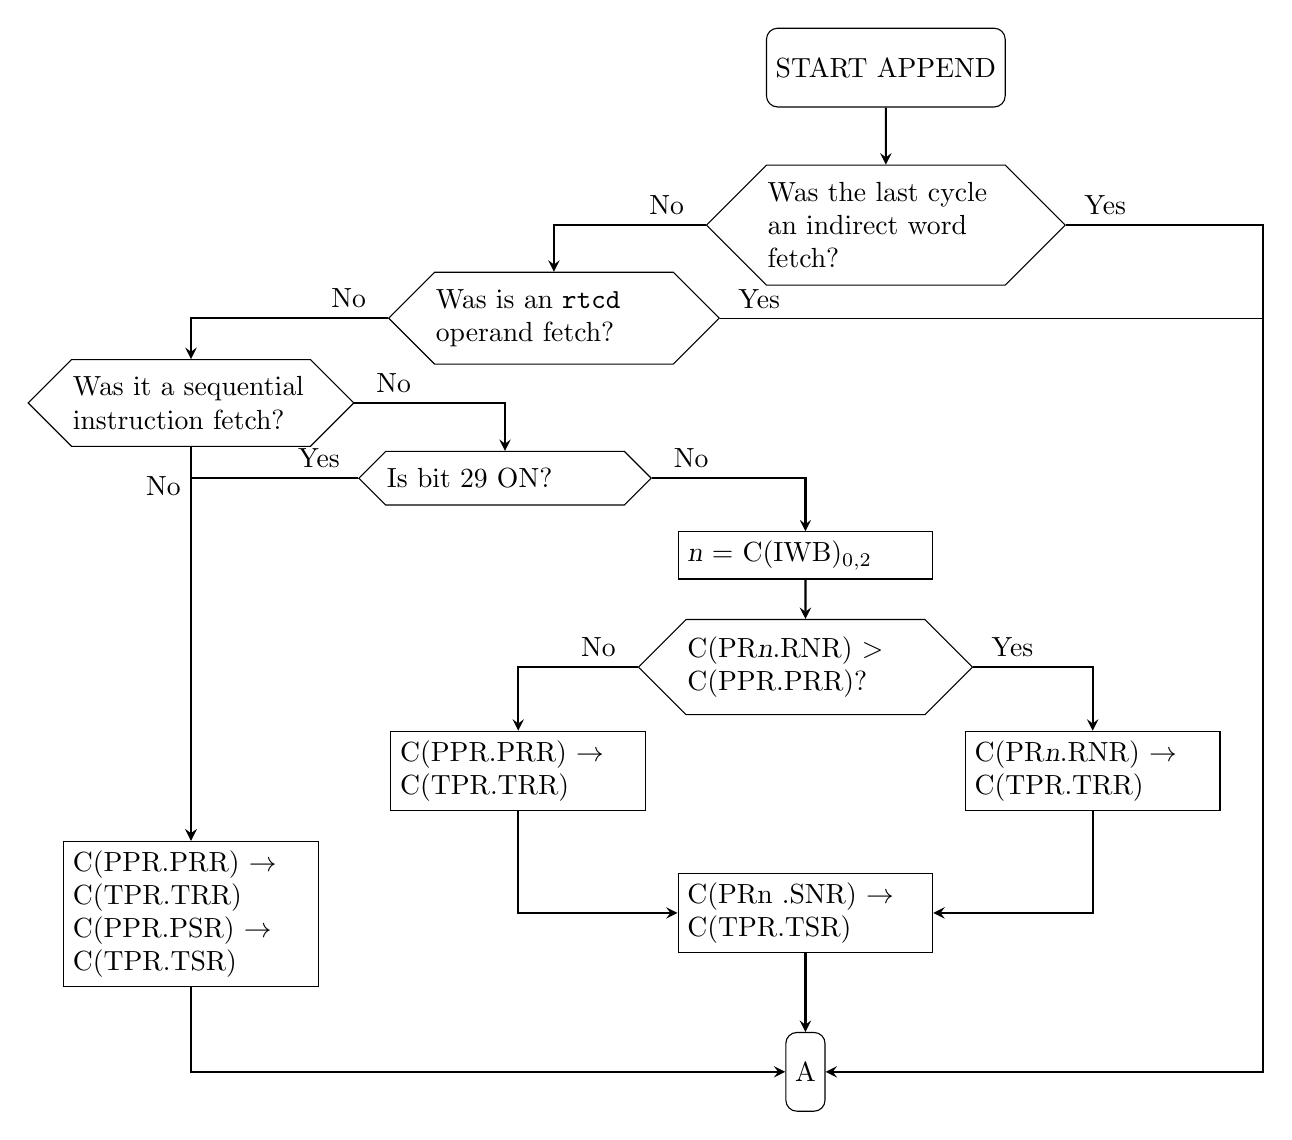
\begin{tikzpicture}[node distance=2cm]
o
\node (start) [startstop] {START APPEND};
\node (wasind) [decision, below of=start] {Was the last cycle an indirect word fetch?};
\node (corner) [coordinate, right=2.5cm of wasind] {};
\node (edge) [coordinate, below=1cm of corner] {};
\node (wasrtcd) [decision, below left=0.5cm and 0.5cm of wasind] {Was is an \texttt{rtcd} operand fetch?};
\node (wasinst) [decision, below left=0.5cm and 1cm of wasrtcd] {Was it a sequential instruction fetch?};
\node (isb29) [decision, below right=0.5cm and .5cm of wasinst] {Is bit 29 ON?};
\node (neq) [process, below right=0.5cm and 0.5cm of isb29] {\textsl{n} = C(IWB)\tsb{0,2}};
\node (isring) [decision, below=0.5cm of neq] {C(PR\textsl{n}.RNR) $>$ C(PPR.PRR)?};
\node (pprring) [process, below left=0.5cm and 0.2cm of isring] {C(PPR.PRR) $\rightarrow$ C(TPR.TRR)};
\node (prnring) [process, below right=0.5cm and 0.2cm of isring] {C(PR\textsl{n}.RNR) $\rightarrow$ C(TPR.TRR)};
\node (settsr) [process, below=2cm of isring] {C(PRn .SNR) $\rightarrow$ C(TPR.TSR)};
\node (useppr) [process, below=5cm of wasinst] {C(PPR.PRR) $\rightarrow$ C(TPR.TRR)\\ C(PPR.PSR) $\rightarrow$ C(TPR.TSR)};
\node (a) [startstop, below=1cm of settsr] {A};

\draw [arrow] (start) -- (wasind);
\draw [arrow] (wasind.west) -- ++ (-1,0) node[anchor=south,pos=0.5] {No} -| (wasrtcd);
\draw [arrow] (wasind.east) -- ++ (1,0) node[anchor=south,pos=0.5] {Yes} -- (corner) |- (a);
\draw [arrow] (wasrtcd.west) -- ++ (-1,0) node[anchor=south,pos=0.5] {No} -| (wasinst);
\draw (wasrtcd.east) -- ++ (1,0) node[anchor=south,pos=0.5] {Yes} -- (wasrtcd-|corner.south);
\draw [arrow] (wasinst.east) -- ++ (1,0) node[anchor=south,pos=0.5] {No} -| (isb29);
\draw [arrow] (isb29.east) -- ++ (1,0) node[anchor=south,pos=0.5] {No} -| (neq);
\draw [arrow] (neq.south) -- (isring);
\draw [arrow] (isring.west) -- ++ (-1,0) node[anchor=south,pos=0.5] {No} -| (pprring);
\draw [arrow] (isring.east) -- ++ (1,0) node[anchor=south,pos=0.5] {Yes} -| (prnring);
\draw [arrow] (pprring.south) |-(settsr);
\draw [arrow] (prnring.south) |- (settsr);
\draw [arrow] (wasinst.south) -- ++ (0,-1) node[anchor=east,pos=0.5] {No} -- (useppr);
\draw [arrow] (isb29.west) -- ++ (-1,0) node[anchor=south,pos=0.5] {Yes} -| (useppr);
\draw [arrow] (useppr.south) |- (a);
\draw [arrow] (settsr.south) -- (a);
\end{tikzpicture}
\caption{ Complete Appending Unit Operation Flowchart}
\label{f8.1}
\end{figure}



\section{DPS/L68 CACHE MEMORY OPERATION}

%% ===== \end{flushleft}
%% ===== 
%% ===== 
%% ===== \begin{flushleft}
%% ===== The Multics processor may be fitted with an optional cache memory. The operation of this
%% ===== \end{flushleft}
%% ===== 
%% ===== 
%% ===== \begin{flushleft}
%% ===== cache memory is described in this section.
%% ===== \end{flushleft}
%% ===== 
%% ===== 
%% ===== 
%% ===== 
%% ===== 
%% ===== \begin{flushleft}

\subsection{PHILOSOPHY OF CACHE MEMORY}

%% ===== \end{flushleft}
%% ===== 
%% ===== 
%% ===== \begin{flushleft}
%% ===== The cache memory is a high speed buffer memory located within the processor that is
%% ===== \end{flushleft}
%% ===== 
%% ===== 
%% ===== \begin{flushleft}
%% ===== intended to hold operands and/or instructions in expectation of their immediate use. This concept
%% ===== \end{flushleft}
%% ===== 
%% ===== 
%% ===== \begin{flushleft}
%% ===== is different from that of holding a single operand (such as the divisor for a divide instruction) in the
%% ===== \end{flushleft}
%% ===== 
%% ===== 
%% ===== \begin{flushleft}
%% ===== processor during execution of a single instruction. A cache memory depends on the locality of
%% ===== \end{flushleft}
%% ===== 
%% ===== 
%% ===== \begin{flushleft}
%% ===== reference principle. Locality of reference involves the calculation of the probability, for any value
%% ===== \end{flushleft}
%% ===== 
%% ===== 
%% ===== \begin{flushleft}
%% ===== of d, that the next instruction or operand reference after a reference to the instruction or operand
%% ===== \end{flushleft}
%% ===== 
%% ===== 
%% ===== \begin{flushleft}
%% ===== at location A is to location A+d.
%% ===== \end{flushleft}
%% ===== 
%% ===== 
%% ===== \begin{flushleft}
%% ===== The calculation of probabilities for a set of values of d requires the statistical analysis of
%% ===== \end{flushleft}
%% ===== 
%% ===== 
%% ===== \begin{flushleft}
%% ===== large volumes of real and simulated instruction sequences and data organizations. If it can be
%% ===== \end{flushleft}
%% ===== 
%% ===== 
%% ===== \begin{flushleft}
%% ===== shown that the average expected data/instruction access time reduction (over the range 1 to d) is
%% ===== \end{flushleft}
%% ===== 
%% ===== 
%% ===== \begin{flushleft}
%% ===== statistically significant in comparison to the fixed main memory access time, then the
%% ===== \end{flushleft}
%% ===== 
%% ===== 
%% ===== \begin{flushleft}
%% ===== implementation of a cache memory with block size d will contribute a significant improvement in
%% ===== \end{flushleft}
%% ===== 
%% ===== 
%% ===== \begin{flushleft}
%% ===== performance.
%% ===== \end{flushleft}
%% ===== 
%% ===== 
%% ===== \begin{flushleft}
%% ===== The results of such studies for the Multics processor with a cache memory as described
%% ===== \end{flushleft}
%% ===== 
%% ===== 
%% ===== \begin{flushleft}
%% ===== below (with d!=!4) show a hit probability ranging between 80 and 95 percent (depending on
%% ===== \end{flushleft}
%% ===== 
%% ===== 
%% ===== \begin{flushleft}
%% ===== instruction mix and data organization) and a performance improvement ranging up to 30 percent.
%% ===== \end{flushleft}
%% ===== 
%% ===== 
%% ===== 
%% ===== 
%% ===== 
%% ===== \begin{flushleft}

\subsection{CACHE MEMORY ORGANIZATION}

%% ===== \end{flushleft}
%% ===== 
%% ===== 
%% ===== \begin{flushleft}
%% ===== The cache memory is implemented as 2048 36-bit words of high-speed register storage with
%% ===== \end{flushleft}
%% ===== 
%% ===== 
%% ===== \begin{flushleft}
%% ===== associated control and content directory circuitry within the processor. It is fully integrated with
%% ===== \end{flushleft}
%% ===== 
%% ===== 
%% ===== \begin{flushleft}
%% ===== the normal data path circuitry and is virtually invisible to all programming sequences. Parity is
%% ===== \end{flushleft}
%% ===== 
%% ===== 
%% ===== \begin{flushleft}
%% ===== generated, stored, and/or checked on each data reference. The total storage is divided into 512
%% ===== \end{flushleft}
%% ===== 
%% ===== 
%% ===== \begin{flushleft}
%% ===== blocks of 4 words each and the blocks are organized into 128 columns of four levels each.
%% ===== \end{flushleft}
%% ===== 
%% ===== 
%% ===== 
%% ===== 
%% ===== 
%% ===== \begin{flushleft}

\subsubsection{Cache Memory / Main Memory Mapping}

%% ===== \end{flushleft}
%% ===== 
%% ===== 
%% ===== \begin{flushleft}
%% ===== Main memory is mapped into the cache memory as described below and shown in Figure
%% ===== \end{flushleft}
%% ===== 
%% ===== 
%% ===== 9-1.
%% ===== 
%% ===== 
%% ===== \begin{flushleft}
%% ===== Main memory is divided into N blocks of 4 words each arranged in ascending order
%% ===== \end{flushleft}
%% ===== 
%% ===== 
%% ===== \begin{flushleft}
%% ===== and numbered with the value of Y15,21 of the first word of the block.
%% ===== \end{flushleft}
%% ===== 
%% ===== 
%% ===== \begin{flushleft}
%% ===== All main memory blocks with numbers n modulo 128 are grouped associatively with
%% ===== \end{flushleft}
%% ===== 
%% ===== 
%% ===== \begin{flushleft}
%% ===== cache memory column n.
%% ===== \end{flushleft}
%% ===== 
%% ===== 
%% ===== \begin{flushleft}
%% ===== Each cache memory column may hold any four blocks of the associated set of main
%% ===== \end{flushleft}
%% ===== 
%% ===== 
%% ===== \begin{flushleft}
%% ===== memory blocks.
%% ===== \end{flushleft}
%% ===== 
%% ===== 
%% ===== \begin{flushleft}
%% ===== Each cache memory column has associated with it a four entry directory (one entry for
%% ===== \end{flushleft}
%% ===== 
%% ===== 
%% ===== \begin{flushleft}
%% ===== each level) and a 2-bit round robin counter. Parity is generated, stored, and checked
%% ===== \end{flushleft}
%% ===== 
%% ===== 
%% ===== \begin{flushleft}
%% ===== on each directory entry.
%% ===== \end{flushleft}
%% ===== 
%% ===== 
%% ===== \begin{flushleft}
%% ===== A cache directory entry consists of a 15-bit ADDRESS register, a pre-set, 2-bit level
%% ===== \end{flushleft}
%% ===== 
%% ===== 
%% ===== \begin{flushleft}
%% ===== number value and a level full flag bit.
%% ===== \end{flushleft}
%% ===== 
%% ===== 
%% ===== 
%% ===== 
%% ===== 
%% ===== \begin{flushleft}
%% ===== \newpage
%% ===== When a main memory block is loaded into a cache memory block at some level in the
%% ===== \end{flushleft}
%% ===== 
%% ===== 
%% ===== \begin{flushleft}
%% ===== associated column, the directory ADDRESS register for that column and level is
%% ===== \end{flushleft}
%% ===== 
%% ===== 
%% ===== \begin{flushleft}
%% ===== loaded with Y0,14. (Level selection is discussed in {``}Cache Memory Control'' later in
%% ===== \end{flushleft}
%% ===== 
%% ===== 
%% ===== \begin{flushleft}
%% ===== this section.)
%% ===== \end{flushleft}
%% ===== 
%% ===== 
%% ===== 
%% ===== 
%% ===== 
%% ===== \begin{flushleft}
%% ===== Main
%% ===== \end{flushleft}
%% ===== 
%% ===== 
%% ===== \begin{flushleft}
%% ===== Memory
%% ===== \end{flushleft}
%% ===== 
%% ===== 
%% ===== 
%% ===== 
%% ===== 
%% ===== \begin{flushleft}
%% ===== Block
%% ===== \end{flushleft}
%% ===== 
%% ===== 
%% ===== 0
%% ===== 
%% ===== 
%% ===== \begin{flushleft}
%% ===== Words
%% ===== \end{flushleft}
%% ===== 
%% ===== 
%% ===== 0,3
%% ===== 
%% ===== 
%% ===== 
%% ===== 
%% ===== 
%% ===== \begin{flushleft}
%% ===== Block
%% ===== \end{flushleft}
%% ===== 
%% ===== 
%% ===== 1
%% ===== 
%% ===== 
%% ===== \begin{flushleft}
%% ===== Words
%% ===== \end{flushleft}
%% ===== 
%% ===== 
%% ===== 4,7
%% ===== 
%% ===== 
%% ===== 
%% ===== 
%% ===== 
%% ===== \begin{flushleft}
%% ===== Block
%% ===== \end{flushleft}
%% ===== 
%% ===== 
%% ===== 2
%% ===== 
%% ===== 
%% ===== \begin{flushleft}
%% ===== Words
%% ===== \end{flushleft}
%% ===== 
%% ===== 
%% ===== 8,11
%% ===== 
%% ===== 
%% ===== 
%% ===== 
%% ===== 
%% ===== \begin{flushleft}
%% ===== Block
%% ===== \end{flushleft}
%% ===== 
%% ===== 
%% ===== 128
%% ===== 
%% ===== 
%% ===== \begin{flushleft}
%% ===== Words
%% ===== \end{flushleft}
%% ===== 
%% ===== 
%% ===== 512,515
%% ===== 
%% ===== 
%% ===== 
%% ===== 
%% ===== 
%% ===== \begin{flushleft}
%% ===== Block
%% ===== \end{flushleft}
%% ===== 
%% ===== 
%% ===== 129
%% ===== 
%% ===== 
%% ===== \begin{flushleft}
%% ===== Words
%% ===== \end{flushleft}
%% ===== 
%% ===== 
%% ===== 516,519
%% ===== 
%% ===== 
%% ===== 
%% ===== 
%% ===== 
%% ===== ...
%% ===== 
%% ===== 
%% ===== 
%% ===== 
%% ===== 
%% ===== \begin{flushleft}
%% ===== Block
%% ===== \end{flushleft}
%% ===== 
%% ===== 
%% ===== \begin{flushleft}
%% ===== N-128
%% ===== \end{flushleft}
%% ===== 
%% ===== 
%% ===== \begin{flushleft}
%% ===== Words
%% ===== \end{flushleft}
%% ===== 
%% ===== 
%% ===== -512,-509
%% ===== 
%% ===== 
%% ===== 
%% ===== 
%% ===== 
%% ===== ...
%% ===== 
%% ===== 
%% ===== 
%% ===== 
%% ===== 
%% ===== \begin{flushleft}
%% ===== Block
%% ===== \end{flushleft}
%% ===== 
%% ===== 
%% ===== \begin{flushleft}
%% ===== N-127
%% ===== \end{flushleft}
%% ===== 
%% ===== 
%% ===== \begin{flushleft}
%% ===== Words
%% ===== \end{flushleft}
%% ===== 
%% ===== 
%% ===== -508,-505
%% ===== 
%% ===== 
%% ===== 
%% ===== 
%% ===== 
%% ===== ...
%% ===== 
%% ===== 
%% ===== 
%% ===== 
%% ===== 
%% ===== \begin{flushleft}
%% ===== Block
%% ===== \end{flushleft}
%% ===== 
%% ===== 
%% ===== 126
%% ===== 
%% ===== 
%% ===== \begin{flushleft}
%% ===== Words
%% ===== \end{flushleft}
%% ===== 
%% ===== 
%% ===== 504,507
%% ===== 
%% ===== 
%% ===== 
%% ===== 
%% ===== 
%% ===== \begin{flushleft}
%% ===== Block
%% ===== \end{flushleft}
%% ===== 
%% ===== 
%% ===== 127
%% ===== 
%% ===== 
%% ===== \begin{flushleft}
%% ===== Words
%% ===== \end{flushleft}
%% ===== 
%% ===== 
%% ===== 508,511
%% ===== 
%% ===== 
%% ===== 
%% ===== 
%% ===== 
%% ===== \begin{flushleft}
%% ===== Block
%% ===== \end{flushleft}
%% ===== 
%% ===== 
%% ===== 130
%% ===== 
%% ===== 
%% ===== \begin{flushleft}
%% ===== Words
%% ===== \end{flushleft}
%% ===== 
%% ===== 
%% ===== 520,523
%% ===== 
%% ===== 
%% ===== 
%% ===== 
%% ===== 
%% ===== ...
%% ===== 
%% ===== 
%% ===== 
%% ===== 
%% ===== 
%% ===== \begin{flushleft}
%% ===== Block
%% ===== \end{flushleft}
%% ===== 
%% ===== 
%% ===== 254
%% ===== 
%% ===== 
%% ===== \begin{flushleft}
%% ===== Words
%% ===== \end{flushleft}
%% ===== 
%% ===== 
%% ===== 1016,1019
%% ===== 
%% ===== 
%% ===== 
%% ===== 
%% ===== 
%% ===== \begin{flushleft}
%% ===== Block
%% ===== \end{flushleft}
%% ===== 
%% ===== 
%% ===== 255
%% ===== 
%% ===== 
%% ===== \begin{flushleft}
%% ===== Words
%% ===== \end{flushleft}
%% ===== 
%% ===== 
%% ===== 1020,1023
%% ===== 
%% ===== 
%% ===== 
%% ===== 
%% ===== 
%% ===== ...
%% ===== 
%% ===== 
%% ===== 
%% ===== 
%% ===== 
%% ===== ...
%% ===== 
%% ===== 
%% ===== 
%% ===== 
%% ===== 
%% ===== ...
%% ===== 
%% ===== 
%% ===== 
%% ===== 
%% ===== 
%% ===== \begin{flushleft}
%% ===== Block
%% ===== \end{flushleft}
%% ===== 
%% ===== 
%% ===== \begin{flushleft}
%% ===== N-126
%% ===== \end{flushleft}
%% ===== 
%% ===== 
%% ===== \begin{flushleft}
%% ===== Words
%% ===== \end{flushleft}
%% ===== 
%% ===== 
%% ===== -504,-501
%% ===== 
%% ===== 
%% ===== 
%% ===== 
%% ===== 
%% ===== ...
%% ===== 
%% ===== 
%% ===== 
%% ===== 
%% ===== 
%% ===== ...
%% ===== 
%% ===== 
%% ===== 
%% ===== 
%% ===== 
%% ===== \begin{flushleft}
%% ===== Block
%% ===== \end{flushleft}
%% ===== 
%% ===== 
%% ===== \begin{flushleft}
%% ===== N-2
%% ===== \end{flushleft}
%% ===== 
%% ===== 
%% ===== \begin{flushleft}
%% ===== Words
%% ===== \end{flushleft}
%% ===== 
%% ===== 
%% ===== -8,-5
%% ===== 
%% ===== 
%% ===== 
%% ===== 
%% ===== 
%% ===== \begin{flushleft}
%% ===== Block
%% ===== \end{flushleft}
%% ===== 
%% ===== 
%% ===== \begin{flushleft}
%% ===== N-1
%% ===== \end{flushleft}
%% ===== 
%% ===== 
%% ===== \begin{flushleft}
%% ===== Words
%% ===== \end{flushleft}
%% ===== 
%% ===== 
%% ===== -4,-1
%% ===== 
%% ===== 
%% ===== 
%% ===== 
%% ===== 
%% ===== \begin{flushleft}
%% ===== Column
%% ===== \end{flushleft}
%% ===== 
%% ===== 
%% ===== 127
%% ===== 
%% ===== 
%% ===== \begin{flushleft}
%% ===== Level
%% ===== \end{flushleft}
%% ===== 
%% ===== 
%% ===== 0
%% ===== 
%% ===== 
%% ===== 
%% ===== 
%% ===== 
%% ===== ...
%% ===== 
%% ===== 
%% ===== 
%% ===== 
%% ===== 
%% ===== \begin{flushleft}
%% ===== Cache
%% ===== \end{flushleft}
%% ===== 
%% ===== 
%% ===== \begin{flushleft}
%% ===== Memory
%% ===== \end{flushleft}
%% ===== 
%% ===== 
%% ===== 
%% ===== 
%% ===== 
%% ===== \begin{flushleft}
%% ===== Column
%% ===== \end{flushleft}
%% ===== 
%% ===== 
%% ===== 0
%% ===== 
%% ===== 
%% ===== \begin{flushleft}
%% ===== Level
%% ===== \end{flushleft}
%% ===== 
%% ===== 
%% ===== 0
%% ===== 
%% ===== 
%% ===== 
%% ===== 
%% ===== 
%% ===== \begin{flushleft}
%% ===== Column
%% ===== \end{flushleft}
%% ===== 
%% ===== 
%% ===== 1
%% ===== 
%% ===== 
%% ===== \begin{flushleft}
%% ===== Level
%% ===== \end{flushleft}
%% ===== 
%% ===== 
%% ===== 0
%% ===== 
%% ===== 
%% ===== 
%% ===== 
%% ===== 
%% ===== \begin{flushleft}
%% ===== Column
%% ===== \end{flushleft}
%% ===== 
%% ===== 
%% ===== 2
%% ===== 
%% ===== 
%% ===== \begin{flushleft}
%% ===== Level
%% ===== \end{flushleft}
%% ===== 
%% ===== 
%% ===== 0
%% ===== 
%% ===== 
%% ===== 
%% ===== 
%% ===== 
%% ===== ...
%% ===== 
%% ===== 
%% ===== 
%% ===== 
%% ===== 
%% ===== \begin{flushleft}
%% ===== Column
%% ===== \end{flushleft}
%% ===== 
%% ===== 
%% ===== 126
%% ===== 
%% ===== 
%% ===== \begin{flushleft}
%% ===== Level
%% ===== \end{flushleft}
%% ===== 
%% ===== 
%% ===== 0
%% ===== 
%% ===== 
%% ===== 
%% ===== 
%% ===== 
%% ===== \begin{flushleft}
%% ===== Column
%% ===== \end{flushleft}
%% ===== 
%% ===== 
%% ===== 0
%% ===== 
%% ===== 
%% ===== \begin{flushleft}
%% ===== Level
%% ===== \end{flushleft}
%% ===== 
%% ===== 
%% ===== 1
%% ===== 
%% ===== 
%% ===== 
%% ===== 
%% ===== 
%% ===== \begin{flushleft}
%% ===== Column
%% ===== \end{flushleft}
%% ===== 
%% ===== 
%% ===== 1
%% ===== 
%% ===== 
%% ===== \begin{flushleft}
%% ===== Level
%% ===== \end{flushleft}
%% ===== 
%% ===== 
%% ===== 1
%% ===== 
%% ===== 
%% ===== 
%% ===== 
%% ===== 
%% ===== \begin{flushleft}
%% ===== Column
%% ===== \end{flushleft}
%% ===== 
%% ===== 
%% ===== 2
%% ===== 
%% ===== 
%% ===== \begin{flushleft}
%% ===== Level
%% ===== \end{flushleft}
%% ===== 
%% ===== 
%% ===== 1
%% ===== 
%% ===== 
%% ===== 
%% ===== 
%% ===== 
%% ===== ...
%% ===== 
%% ===== 
%% ===== 
%% ===== 
%% ===== 
%% ===== \begin{flushleft}
%% ===== Column
%% ===== \end{flushleft}
%% ===== 
%% ===== 
%% ===== 126
%% ===== 
%% ===== 
%% ===== \begin{flushleft}
%% ===== Level
%% ===== \end{flushleft}
%% ===== 
%% ===== 
%% ===== 1
%% ===== 
%% ===== 
%% ===== 
%% ===== 
%% ===== 
%% ===== \begin{flushleft}
%% ===== Column
%% ===== \end{flushleft}
%% ===== 
%% ===== 
%% ===== 127
%% ===== 
%% ===== 
%% ===== \begin{flushleft}
%% ===== Level
%% ===== \end{flushleft}
%% ===== 
%% ===== 
%% ===== 1
%% ===== 
%% ===== 
%% ===== 
%% ===== 
%% ===== 
%% ===== \begin{flushleft}
%% ===== Column
%% ===== \end{flushleft}
%% ===== 
%% ===== 
%% ===== 0
%% ===== 
%% ===== 
%% ===== \begin{flushleft}
%% ===== Level
%% ===== \end{flushleft}
%% ===== 
%% ===== 
%% ===== 2
%% ===== 
%% ===== 
%% ===== 
%% ===== 
%% ===== 
%% ===== \begin{flushleft}
%% ===== Column
%% ===== \end{flushleft}
%% ===== 
%% ===== 
%% ===== 1
%% ===== 
%% ===== 
%% ===== \begin{flushleft}
%% ===== Level
%% ===== \end{flushleft}
%% ===== 
%% ===== 
%% ===== 2
%% ===== 
%% ===== 
%% ===== 
%% ===== 
%% ===== 
%% ===== \begin{flushleft}
%% ===== Column
%% ===== \end{flushleft}
%% ===== 
%% ===== 
%% ===== 2
%% ===== 
%% ===== 
%% ===== \begin{flushleft}
%% ===== Level
%% ===== \end{flushleft}
%% ===== 
%% ===== 
%% ===== 2
%% ===== 
%% ===== 
%% ===== 
%% ===== 
%% ===== 
%% ===== ...
%% ===== 
%% ===== 
%% ===== 
%% ===== 
%% ===== 
%% ===== \begin{flushleft}
%% ===== Column
%% ===== \end{flushleft}
%% ===== 
%% ===== 
%% ===== 126
%% ===== 
%% ===== 
%% ===== \begin{flushleft}
%% ===== Level
%% ===== \end{flushleft}
%% ===== 
%% ===== 
%% ===== 2
%% ===== 
%% ===== 
%% ===== 
%% ===== 
%% ===== 
%% ===== \begin{flushleft}
%% ===== Column
%% ===== \end{flushleft}
%% ===== 
%% ===== 
%% ===== 127
%% ===== 
%% ===== 
%% ===== \begin{flushleft}
%% ===== Level
%% ===== \end{flushleft}
%% ===== 
%% ===== 
%% ===== 2
%% ===== 
%% ===== 
%% ===== 
%% ===== 
%% ===== 
%% ===== \begin{flushleft}
%% ===== Column
%% ===== \end{flushleft}
%% ===== 
%% ===== 
%% ===== 0
%% ===== 
%% ===== 
%% ===== \begin{flushleft}
%% ===== Level
%% ===== \end{flushleft}
%% ===== 
%% ===== 
%% ===== 3
%% ===== 
%% ===== 
%% ===== 
%% ===== 
%% ===== 
%% ===== \begin{flushleft}
%% ===== Column
%% ===== \end{flushleft}
%% ===== 
%% ===== 
%% ===== 1
%% ===== 
%% ===== 
%% ===== \begin{flushleft}
%% ===== Level
%% ===== \end{flushleft}
%% ===== 
%% ===== 
%% ===== 3
%% ===== 
%% ===== 
%% ===== 
%% ===== 
%% ===== 
%% ===== \begin{flushleft}
%% ===== Column
%% ===== \end{flushleft}
%% ===== 
%% ===== 
%% ===== 2
%% ===== 
%% ===== 
%% ===== \begin{flushleft}
%% ===== Level
%% ===== \end{flushleft}
%% ===== 
%% ===== 
%% ===== 3
%% ===== 
%% ===== 
%% ===== 
%% ===== 
%% ===== 
%% ===== ...
%% ===== 
%% ===== 
%% ===== 
%% ===== 
%% ===== 
%% ===== \begin{flushleft}
%% ===== Column
%% ===== \end{flushleft}
%% ===== 
%% ===== 
%% ===== 126
%% ===== 
%% ===== 
%% ===== \begin{flushleft}
%% ===== Level
%% ===== \end{flushleft}
%% ===== 
%% ===== 
%% ===== 3
%% ===== 
%% ===== 
%% ===== 
%% ===== 
%% ===== 
%% ===== \begin{flushleft}
%% ===== Column
%% ===== \end{flushleft}
%% ===== 
%% ===== 
%% ===== 127
%% ===== 
%% ===== 
%% ===== \begin{flushleft}
%% ===== Level
%% ===== \end{flushleft}
%% ===== 
%% ===== 
%% ===== 3
%% ===== 
%% ===== 
%% ===== 
%% ===== 
%% ===== 
%% ===== \begin{flushleft}
%% ===== Figure 9-1. Main Memory/Cache Memory Mapping
%% ===== \end{flushleft}
%% ===== 
%% ===== 
%% ===== 
%% ===== 
%% ===== 
%% ===== \begin{flushleft}

\subsubsection{Cache Memory Addressing}

%% ===== \end{flushleft}
%% ===== 
%% ===== 
%% ===== \begin{flushleft}
%% ===== For a read operation, the 24-bit absolute main memory address prepared by the appending
%% ===== \end{flushleft}
%% ===== 
%% ===== 
%% ===== \begin{flushleft}
%% ===== unit is presented simultaneously to the cache control and to the main memory port selection
%% ===== \end{flushleft}
%% ===== 
%% ===== 
%% ===== \begin{flushleft}
%% ===== circuitry. While port selection is being accomplished, the cache memory is accessed as follows.
%% ===== \end{flushleft}
%% ===== 
%% ===== 
%% ===== \begin{flushleft}
%% ===== Yl5,21 are used to select a cache memory column.
%% ===== \end{flushleft}
%% ===== 
%% ===== 
%% ===== 
%% ===== 
%% ===== 
%% ===== \begin{flushleft}
%% ===== \newpage
%% ===== Y0,14 are matched associatively against the four directory ADDRESS registers for the
%% ===== \end{flushleft}
%% ===== 
%% ===== 
%% ===== \begin{flushleft}
%% ===== selected column.
%% ===== \end{flushleft}
%% ===== 
%% ===== 
%% ===== \begin{flushleft}
%% ===== If a match occurs for a level whose full flag is ON, a hit is signaled, the main memory
%% ===== \end{flushleft}
%% ===== 
%% ===== 
%% ===== \begin{flushleft}
%% ===== reference cycle is canceled, and the level number value is read out.
%% ===== \end{flushleft}
%% ===== 
%% ===== 
%% ===== \begin{flushleft}
%% ===== The level number value and Y22,23 are used to select the level and word in the selected
%% ===== \end{flushleft}
%% ===== 
%% ===== 
%% ===== \begin{flushleft}
%% ===== column and the cache memory data is read out into the data circuitry.
%% ===== \end{flushleft}
%% ===== 
%% ===== 
%% ===== \begin{flushleft}
%% ===== If no hit is signaled, the main memory reference cycle proceeds and a cache memory
%% ===== \end{flushleft}
%% ===== 
%% ===== 
%% ===== \begin{flushleft}
%% ===== block load cycle is initiated (see {``}Cache Memory Control'' below).
%% ===== \end{flushleft}
%% ===== 
%% ===== 
%% ===== \begin{flushleft}
%% ===== For a write operation, the 24-bit absolute main memory address prepared by the appending
%% ===== \end{flushleft}
%% ===== 
%% ===== 
%% ===== \begin{flushleft}
%% ===== unit is presented simultaneously to the cache control and to the main memory port selection
%% ===== \end{flushleft}
%% ===== 
%% ===== 
%% ===== \begin{flushleft}
%% ===== circuitry. While port selection is being accomplished, the cache memory is accessed as follows.
%% ===== \end{flushleft}
%% ===== 
%% ===== 
%% ===== \begin{flushleft}
%% ===== Y15,21 are used to select a cache memory column.
%% ===== \end{flushleft}
%% ===== 
%% ===== 
%% ===== \begin{flushleft}
%% ===== Y0,14 are matched associatively against the four directory ADDRESS registers for the
%% ===== \end{flushleft}
%% ===== 
%% ===== 
%% ===== \begin{flushleft}
%% ===== selected column.
%% ===== \end{flushleft}
%% ===== 
%% ===== 
%% ===== \begin{flushleft}
%% ===== If a match occurs for a level whose full flag is ON, a hit is signaled and the level
%% ===== \end{flushleft}
%% ===== 
%% ===== 
%% ===== \begin{flushleft}
%% ===== number value is read out.
%% ===== \end{flushleft}
%% ===== 
%% ===== 
%% ===== \begin{flushleft}
%% ===== The level number value and Y22,23 are used to select the level and word in the selected
%% ===== \end{flushleft}
%% ===== 
%% ===== 
%% ===== \begin{flushleft}
%% ===== column, a cache memory write cycle is enabled, and the data is written to the main
%% ===== \end{flushleft}
%% ===== 
%% ===== 
%% ===== \begin{flushleft}
%% ===== memory and the cache memory simultaneously.
%% ===== \end{flushleft}
%% ===== 
%% ===== 
%% ===== \begin{flushleft}
%% ===== If no hit is signaled, the main memory reference cycle proceeds with no further cache
%% ===== \end{flushleft}
%% ===== 
%% ===== 
%% ===== \begin{flushleft}
%% ===== memory action.
%% ===== \end{flushleft}
%% ===== 
%% ===== 
%% ===== 
%% ===== 
%% ===== 
%% ===== \begin{flushleft}
%% ===== \newpage

\subsection{CACHE MEMORY CONTROL}

%% ===== \end{flushleft}
%% ===== 
%% ===== 
%% ===== \begin{flushleft}

\subsubsection{Enabling and Disabling Cache Memory}

%% ===== \end{flushleft}
%% ===== 
%% ===== 
%% ===== \begin{flushleft}
%% ===== The cache memory is controlled by the state of several bits in the cache mode register (see
%% ===== \end{flushleft}
%% ===== 
%% ===== 
%% ===== \begin{flushleft}
%% ===== Section 3). The cache mode register may be loaded with the Load Central Processor Register
%% ===== \end{flushleft}
%% ===== 
%% ===== 
%% ===== \begin{flushleft}
%% ===== (lcpr) instruction. The cache memory control bits are as follows:
%% ===== \end{flushleft}
%% ===== 
%% ===== 
%% ===== 
%% ===== 
%% ===== 
%% ===== \begin{flushleft}
%% ===== bit
%% ===== \end{flushleft}
%% ===== 
%% ===== 
%% ===== 54
%% ===== 
%% ===== 
%% ===== 
%% ===== 
%% ===== 
%% ===== 55
%% ===== 
%% ===== 
%% ===== 
%% ===== 
%% ===== 
%% ===== 56
%% ===== 
%% ===== 
%% ===== 57
%% ===== 
%% ===== 
%% ===== 59
%% ===== 
%% ===== 
%% ===== 
%% ===== 
%% ===== 
%% ===== \begin{flushleft}
%% ===== NOTE:
%% ===== \end{flushleft}
%% ===== 
%% ===== 
%% ===== 
%% ===== 
%% ===== 
%% ===== \begin{flushleft}
%% ===== Value Action
%% ===== \end{flushleft}
%% ===== 
%% ===== 
%% ===== 0
%% ===== 
%% ===== 
%% ===== 
%% ===== 
%% ===== 
%% ===== \begin{flushleft}
%% ===== The lower half of the cache memory (levels 0 and 1) is disabled.
%% ===== \end{flushleft}
%% ===== 
%% ===== 
%% ===== 
%% ===== 
%% ===== 
%% ===== 1
%% ===== 
%% ===== 
%% ===== 
%% ===== 
%% ===== 
%% ===== \begin{flushleft}
%% ===== The lower half of the cache memory is active and enabled as per the state of bits
%% ===== \end{flushleft}
%% ===== 
%% ===== 
%% ===== 56-57.
%% ===== 
%% ===== 
%% ===== 
%% ===== 
%% ===== 
%% ===== 0
%% ===== 
%% ===== 
%% ===== 
%% ===== 
%% ===== 
%% ===== \begin{flushleft}
%% ===== The upper half of the cache memory (levels 2 and 3) is disabled.
%% ===== \end{flushleft}
%% ===== 
%% ===== 
%% ===== 
%% ===== 
%% ===== 
%% ===== 1
%% ===== 
%% ===== 
%% ===== 
%% ===== 
%% ===== 
%% ===== \begin{flushleft}
%% ===== The upper half of the cache memory is active and enabled as per the state of bits
%% ===== \end{flushleft}
%% ===== 
%% ===== 
%% ===== 56-57.
%% ===== 
%% ===== 
%% ===== 
%% ===== 
%% ===== 
%% ===== 0
%% ===== 
%% ===== 
%% ===== 
%% ===== 
%% ===== 
%% ===== \begin{flushleft}
%% ===== The cache memory (if active) is not used for operands and indirect words.
%% ===== \end{flushleft}
%% ===== 
%% ===== 
%% ===== 
%% ===== 
%% ===== 
%% ===== 1
%% ===== 
%% ===== 
%% ===== 
%% ===== 
%% ===== 
%% ===== \begin{flushleft}
%% ===== The cache memory (if active) is used for operands and indirect words.
%% ===== \end{flushleft}
%% ===== 
%% ===== 
%% ===== 
%% ===== 
%% ===== 
%% ===== 0
%% ===== 
%% ===== 
%% ===== 
%% ===== 
%% ===== 
%% ===== \begin{flushleft}
%% ===== The cache memory (if active) is not used for instructions.
%% ===== \end{flushleft}
%% ===== 
%% ===== 
%% ===== 
%% ===== 
%% ===== 
%% ===== 1
%% ===== 
%% ===== 
%% ===== 
%% ===== 
%% ===== 
%% ===== \begin{flushleft}
%% ===== The cache memory (if active) is used for instructions.
%% ===== \end{flushleft}
%% ===== 
%% ===== 
%% ===== 
%% ===== 
%% ===== 
%% ===== 0
%% ===== 
%% ===== 
%% ===== 
%% ===== 
%% ===== 
%% ===== \begin{flushleft}
%% ===== The cache-to-register mode is not in effect (see {``}Dumping the Cache Memory''
%% ===== \end{flushleft}
%% ===== 
%% ===== 
%% ===== \begin{flushleft}
%% ===== later in this section).
%% ===== \end{flushleft}
%% ===== 
%% ===== 
%% ===== 
%% ===== 
%% ===== 
%% ===== 1
%% ===== 
%% ===== 
%% ===== 
%% ===== 
%% ===== 
%% ===== \begin{flushleft}
%% ===== The cache-to-register mode is in effect.
%% ===== \end{flushleft}
%% ===== 
%% ===== 
%% ===== 
%% ===== 
%% ===== 
%% ===== \begin{flushleft}
%% ===== The cache memory option furnishes a switch panel maintenance aid that attaches to the
%% ===== \end{flushleft}
%% ===== 
%% ===== 
%% ===== \begin{flushleft}
%% ===== free edge of the cache memory control logic board. The switch panel provides six
%% ===== \end{flushleft}
%% ===== 
%% ===== 
%% ===== \begin{flushleft}
%% ===== switches for manual control of the cache memory:
%% ===== \end{flushleft}
%% ===== 
%% ===== 
%% ===== \begin{flushleft}
%% ===== Four of the switches inhibit the control functions of bits 54-57 of the cache mode
%% ===== \end{flushleft}
%% ===== 
%% ===== 
%% ===== \begin{flushleft}
%% ===== register and have the effect of forcing the corresponding function to be disabled.
%% ===== \end{flushleft}
%% ===== 
%% ===== 
%% ===== \begin{flushleft}
%% ===== The fifth switch inhibits the store-aside feature wherein the processor is permitted to
%% ===== \end{flushleft}
%% ===== 
%% ===== 
%% ===== \begin{flushleft}
%% ===== proceed immediately after the cache memory write cycle on write operations without
%% ===== \end{flushleft}
%% ===== 
%% ===== 
%% ===== \begin{flushleft}
%% ===== waiting for a data acknowledgment from main memory. (There is no software control
%% ===== \end{flushleft}
%% ===== 
%% ===== 
%% ===== \begin{flushleft}
%% ===== corresponding to this switch).
%% ===== \end{flushleft}
%% ===== 
%% ===== 
%% ===== \begin{flushleft}
%% ===== The sixth switch forces the enabled condition on all cache memory controls (except
%% ===== \end{flushleft}
%% ===== 
%% ===== 
%% ===== \begin{flushleft}
%% ===== cache-to-register mode) without regard to the corresponding cache mode register
%% ===== \end{flushleft}
%% ===== 
%% ===== 
%% ===== \begin{flushleft}
%% ===== control bit.
%% ===== \end{flushleft}
%% ===== 
%% ===== 
%% ===== \begin{flushleft}
%% ===== There is no switch corresponding to the cache-to-register control bit.
%% ===== \end{flushleft}
%% ===== 
%% ===== 
%% ===== \begin{flushleft}
%% ===== While these switches are intended primarily for maintenance sessions, they have been
%% ===== \end{flushleft}
%% ===== 
%% ===== 
%% ===== \begin{flushleft}
%% ===== found useful in testing the cache memory during normal operation and in permitting
%% ===== \end{flushleft}
%% ===== 
%% ===== 
%% ===== \begin{flushleft}
%% ===== operation of the processor with the cache memory in degraded or partially disabled
%% ===== \end{flushleft}
%% ===== 
%% ===== 
%% ===== \begin{flushleft}
%% ===== mode.
%% ===== \end{flushleft}
%% ===== 
%% ===== 
%% ===== 
%% ===== 
%% ===== 
%% ===== \begin{flushleft}

\subsubsection{Cache Memory Control in Segment Descriptor Words}

%% ===== \end{flushleft}
%% ===== 
%% ===== 
%% ===== \begin{flushleft}
%% ===== Certain data have characteristics such that they should never be loaded into the cache
%% ===== \end{flushleft}
%% ===== 
%% ===== 
%% ===== \begin{flushleft}
%% ===== memory. Primary examples of such data are hardware mailboxes for the I/O multiplexer, bulk
%% ===== \end{flushleft}
%% ===== 
%% ===== 
%% ===== \begin{flushleft}
%% ===== store controller, etc., status return words, and various dynamic operating system data base
%% ===== \end{flushleft}
%% ===== 
%% ===== 
%% ===== \begin{flushleft}
%% ===== segments. In general, any data that is modified by an agency external to a processor with the
%% ===== \end{flushleft}
%% ===== 
%% ===== 
%% ===== \begin{flushleft}
%% ===== intent to convey information to that processor should never be loaded into cache memory.
%% ===== \end{flushleft}
%% ===== 
%% ===== 
%% ===== 
%% ===== 
%% ===== 
%% ===== \begin{flushleft}
%% ===== \newpage
%% ===== Bit 57 of the segment descriptor word is used to reflect this property of {``}encacheability'' for
%% ===== \end{flushleft}
%% ===== 
%% ===== 
%% ===== \begin{flushleft}
%% ===== each segment. (See Section 5 for a discussion of the segment descriptor word.) If the bit is set
%% ===== \end{flushleft}
%% ===== 
%% ===== 
%% ===== \begin{flushleft}
%% ===== ON, data from the segment may be loaded into the cache memory; if the bit is OFF, they may not.
%% ===== \end{flushleft}
%% ===== 
%% ===== 
%% ===== \begin{flushleft}
%% ===== The operating system may set bit 57 ON or OFF as appropriate for the use of the segment.
%% ===== \end{flushleft}
%% ===== 
%% ===== 
%% ===== 
%% ===== 
%% ===== 
%% ===== \begin{flushleft}

\subsubsection{Loading the Cache Memory}

%% ===== \end{flushleft}
%% ===== 
%% ===== 
%% ===== \begin{flushleft}
%% ===== The cache memory is loaded with data implicitly whenever a cache memory block load is
%% ===== \end{flushleft}
%% ===== 
%% ===== 
%% ===== \begin{flushleft}
%% ===== required. (See the discussion of read operations in {``}Cache Memory Addressing'' earlier in this
%% ===== \end{flushleft}
%% ===== 
%% ===== 
%% ===== \begin{flushleft}
%% ===== section.) There is no explicit method or instruction to load data into the cache memory.
%% ===== \end{flushleft}
%% ===== 
%% ===== 
%% ===== \begin{flushleft}
%% ===== When a cache memory block load is required, the level is selected from the value of the
%% ===== \end{flushleft}
%% ===== 
%% ===== 
%% ===== \begin{flushleft}
%% ===== round robin counter for the selected column, and the cache memory write function is enabled.
%% ===== \end{flushleft}
%% ===== 
%% ===== 
%% ===== \begin{flushleft}
%% ===== (The round robin counter contains the number of the least recently loaded level.) When the data
%% ===== \end{flushleft}
%% ===== 
%% ===== 
%% ===== \begin{flushleft}
%% ===== arrives from main memory, it is written into the cache memory and entered into the data circuitry.
%% ===== \end{flushleft}
%% ===== 
%% ===== 
%% ===== \begin{flushleft}
%% ===== The processor proceeds with the execution of the instruction requiring the operand if appropriate.
%% ===== \end{flushleft}
%% ===== 
%% ===== 
%% ===== \begin{flushleft}
%% ===== When the cache memory write is complete, further virtual address formation is inhibited,
%% ===== \end{flushleft}
%% ===== 
%% ===== 
%% ===== \begin{flushleft}
%% ===== Y22 is inverted, and a second main memory access for the other half of the block is made. When
%% ===== \end{flushleft}
%% ===== 
%% ===== 
%% ===== \begin{flushleft}
%% ===== the second half data arrives from main memory, it is written into the cache memory, Y0,14 are
%% ===== \end{flushleft}
%% ===== 
%% ===== 
%% ===== \begin{flushleft}
%% ===== loaded into the directory ADDRESS register, the level full flag is set ON, the round robin counter is
%% ===== \end{flushleft}
%% ===== 
%% ===== 
%% ===== \begin{flushleft}
%% ===== advanced by 1, and virtual address formation is permitted to proceed.
%% ===== \end{flushleft}
%% ===== 
%% ===== 
%% ===== \begin{flushleft}
%% ===== If all four level full flags for a column are set ON, a column full flag is also set ON and
%% ===== \end{flushleft}
%% ===== 
%% ===== 
%% ===== \begin{flushleft}
%% ===== remains ON until one or more levels in the column are cleared.
%% ===== \end{flushleft}
%% ===== 
%% ===== 
%% ===== 
%% ===== 
%% ===== 
%% ===== \begin{flushleft}

\subsubsection{Clearing the Cache Memory}

%% ===== \end{flushleft}
%% ===== 
%% ===== 
%% ===== \begin{flushleft}
%% ===== Cache memory can be cleared in two ways; general clear and selective clear. The clearing
%% ===== \end{flushleft}
%% ===== 
%% ===== 
%% ===== \begin{flushleft}
%% ===== action is the same in both cases, namely, the full flags of the selected column(s) and/or level(s) are
%% ===== \end{flushleft}
%% ===== 
%% ===== 
%% ===== \begin{flushleft}
%% ===== set OFF.
%% ===== \end{flushleft}
%% ===== 
%% ===== 
%% ===== 
%% ===== 
%% ===== 
%% ===== \begin{flushleft}

\subsubsubsection{General Clear}

%% ===== \end{flushleft}
%% ===== 
%% ===== 
%% ===== \begin{flushleft}
%% ===== The entire cache memory is cleared by setting all column and level full flags to OFF in the
%% ===== \end{flushleft}
%% ===== 
%% ===== 
%% ===== \begin{flushleft}
%% ===== following situations:
%% ===== \end{flushleft}
%% ===== 
%% ===== 
%% ===== \begin{flushleft}
%% ===== Upper or lower cache memory or both becoming enabled by appropriate bits in the
%% ===== \end{flushleft}
%% ===== 
%% ===== 
%% ===== \begin{flushleft}
%% ===== operand of the Load Central Processor Register (lcpr) instruction or by action of the
%% ===== \end{flushleft}
%% ===== 
%% ===== 
%% ===== \begin{flushleft}
%% ===== cache memory control logic board free edge switches.
%% ===== \end{flushleft}
%% ===== 
%% ===== 
%% ===== \begin{flushleft}
%% ===== Execution of a Clear Associative Memory Segments (cams) instruction with bit 15 of
%% ===== \end{flushleft}
%% ===== 
%% ===== 
%% ===== \begin{flushleft}
%% ===== the address field set ON.
%% ===== \end{flushleft}
%% ===== 
%% ===== 
%% ===== 
%% ===== 
%% ===== 
%% ===== \begin{flushleft}

\subsubsubsection{Selective Clear}

%% ===== \end{flushleft}
%% ===== 
%% ===== 
%% ===== \begin{flushleft}
%% ===== The cache memory is cleared selectively as follows:
%% ===== \end{flushleft}
%% ===== 
%% ===== 
%% ===== \begin{flushleft}
%% ===== If a read-and-clear operation (ldac, sznc, etc.) results in a hit on the cache memory,
%% ===== \end{flushleft}
%% ===== 
%% ===== 
%% ===== \begin{flushleft}
%% ===== that cache memory block hit is cleared.
%% ===== \end{flushleft}
%% ===== 
%% ===== 
%% ===== \begin{flushleft}
%% ===== Execution of a Clear Associative Memory Pages (camp) instruction with address bit 15
%% ===== \end{flushleft}
%% ===== 
%% ===== 
%% ===== \begin{flushleft}
%% ===== set ON causes Y13,14 to be matched against all cache directory ADDRESS registers.
%% ===== \end{flushleft}
%% ===== 
%% ===== 
%% ===== \begin{flushleft}
%% ===== All cache memory blocks hit are cleared.
%% ===== \end{flushleft}
%% ===== 
%% ===== 
%% ===== 
%% ===== 
%% ===== 
%% ===== \begin{flushleft}
%% ===== \newpage

\subsubsection{Dumping the Cache Memory}

%% ===== \end{flushleft}
%% ===== 
%% ===== 
%% ===== \begin{flushleft}
%% ===== When the cache-to-register mode flag (bit 59 of the cache mode register) is set ON, the
%% ===== \end{flushleft}
%% ===== 
%% ===== 
%% ===== \begin{flushleft}
%% ===== processor is forced to fetch the operands of all double-precision operations unit load operations
%% ===== \end{flushleft}
%% ===== 
%% ===== 
%% ===== \begin{flushleft}
%% ===== from the cache memory. Y0,12 are ignored, Y15,21 select a column, and Y13,14 select a level. All
%% ===== \end{flushleft}
%% ===== 
%% ===== 
%% ===== \begin{flushleft}
%% ===== other operations (e.g., instruction fetches, single-precision operands, etc.) are treated normally.
%% ===== \end{flushleft}
%% ===== 
%% ===== 
%% ===== \begin{flushleft}
%% ===== Note that the phrase {``}treated normally'' as used here includes the case where the cache
%% ===== \end{flushleft}
%% ===== 
%% ===== 
%% ===== \begin{flushleft}
%% ===== memory is enabled. If the cache memory is enabled, the {``}other'' operations causes normal block
%% ===== \end{flushleft}
%% ===== 
%% ===== 
%% ===== \begin{flushleft}
%% ===== loads and cache memory writes thus destroying the original contents of the cache memory. The
%% ===== \end{flushleft}
%% ===== 
%% ===== 
%% ===== \begin{flushleft}
%% ===== cache memory should be disabled before dumping is attempted.
%% ===== \end{flushleft}
%% ===== 
%% ===== 
%% ===== \begin{flushleft}
%% ===== An indexed program loop involving the ldaq and staq instructions with the cache-toregister mode bit set ON serves to dump any or all of the cache memory.
%% ===== \end{flushleft}
%% ===== 
%% ===== 
%% ===== \begin{flushleft}
%% ===== The occurrence of a fault or interrupt sets the cache-to-register mode bit to OFF.
%% ===== \end{flushleft}
%% ===== 
%% ===== 
%% ===== 
%% ===== 
%% ===== 

\begin{appendices}
\section{OPERATION CODE MAP}
%% ===== \end{flushleft}
%% ===== 
%% ===== 
%% ===== \begin{flushleft}
%% ===== This appendix contains the operation code map for the processor in Figure A-1. The second
%% ===== \end{flushleft}
%% ===== 
%% ===== 
%% ===== \begin{flushleft}
%% ===== portion of the map includes extended instruction set (EIS) instructions. Also see Appendix B for an
%% ===== \end{flushleft}
%% ===== 
%% ===== 
%% ===== \begin{flushleft}
%% ===== alphabetical instruction list.
%% ===== \end{flushleft}
%% ===== 
%% ===== 
%% ===== 
%% ===== 
%% ===== 
%% ===== \begin{flushleft}
%% ===== \newpage
%% ===== OPERATION CODE MAP (BIT 27 = 0)
%% ===== \end{flushleft}
%% ===== 
%% ===== 
%% ===== 000
%% ===== 
%% ===== 
%% ===== 000
%% ===== 
%% ===== 
%% ===== 020
%% ===== 
%% ===== 
%% ===== 040
%% ===== 
%% ===== 
%% ===== 060
%% ===== 
%% ===== 
%% ===== 100
%% ===== 
%% ===== 
%% ===== 120
%% ===== 
%% ===== 
%% ===== 140
%% ===== 
%% ===== 
%% ===== 160
%% ===== 
%% ===== 
%% ===== 200
%% ===== 
%% ===== 
%% ===== 220
%% ===== 
%% ===== 
%% ===== 240
%% ===== 
%% ===== 
%% ===== 260
%% ===== 
%% ===== 
%% ===== 300
%% ===== 
%% ===== 
%% ===== 320
%% ===== 
%% ===== 
%% ===== 340
%% ===== 
%% ===== 
%% ===== 360
%% ===== 
%% ===== 
%% ===== 400
%% ===== 
%% ===== 
%% ===== 420
%% ===== 
%% ===== 
%% ===== 440
%% ===== 
%% ===== 
%% ===== 460
%% ===== 
%% ===== 
%% ===== 500
%% ===== 
%% ===== 
%% ===== 520
%% ===== 
%% ===== 
%% ===== 540
%% ===== 
%% ===== 
%% ===== 560
%% ===== 
%% ===== 
%% ===== 600
%% ===== 
%% ===== 
%% ===== 620
%% ===== 
%% ===== 
%% ===== 640
%% ===== 
%% ===== 
%% ===== 660
%% ===== 
%% ===== 
%% ===== 700
%% ===== 
%% ===== 
%% ===== 720
%% ===== 
%% ===== 
%% ===== 740
%% ===== 
%% ===== 
%% ===== 760
%% ===== 
%% ===== 
%% ===== 
%% ===== 
%% ===== 
%% ===== \begin{flushleft}
%% ===== adlx0
%% ===== \end{flushleft}
%% ===== 
%% ===== 
%% ===== \begin{flushleft}
%% ===== asx0
%% ===== \end{flushleft}
%% ===== 
%% ===== 
%% ===== \begin{flushleft}
%% ===== adx0
%% ===== \end{flushleft}
%% ===== 
%% ===== 
%% ===== \begin{flushleft}
%% ===== cmpx0
%% ===== \end{flushleft}
%% ===== 
%% ===== 
%% ===== \begin{flushleft}
%% ===== sblx0
%% ===== \end{flushleft}
%% ===== 
%% ===== 
%% ===== \begin{flushleft}
%% ===== ssx0
%% ===== \end{flushleft}
%% ===== 
%% ===== 
%% ===== \begin{flushleft}
%% ===== sbx0
%% ===== \end{flushleft}
%% ===== 
%% ===== 
%% ===== \begin{flushleft}
%% ===== cnax0
%% ===== \end{flushleft}
%% ===== 
%% ===== 
%% ===== \begin{flushleft}
%% ===== ldx0
%% ===== \end{flushleft}
%% ===== 
%% ===== 
%% ===== \begin{flushleft}
%% ===== orsx0
%% ===== \end{flushleft}
%% ===== 
%% ===== 
%% ===== \begin{flushleft}
%% ===== orx0
%% ===== \end{flushleft}
%% ===== 
%% ===== 
%% ===== \begin{flushleft}
%% ===== canx0
%% ===== \end{flushleft}
%% ===== 
%% ===== 
%% ===== \begin{flushleft}
%% ===== lcx0
%% ===== \end{flushleft}
%% ===== 
%% ===== 
%% ===== \begin{flushleft}
%% ===== ansx0
%% ===== \end{flushleft}
%% ===== 
%% ===== 
%% ===== \begin{flushleft}
%% ===== anx0
%% ===== \end{flushleft}
%% ===== 
%% ===== 
%% ===== 
%% ===== 
%% ===== 
%% ===== 001
%% ===== 
%% ===== 
%% ===== \begin{flushleft}
%% ===== mme
%% ===== \end{flushleft}
%% ===== 
%% ===== 
%% ===== \begin{flushleft}
%% ===== adlx1
%% ===== \end{flushleft}
%% ===== 
%% ===== 
%% ===== \begin{flushleft}
%% ===== asx1
%% ===== \end{flushleft}
%% ===== 
%% ===== 
%% ===== \begin{flushleft}
%% ===== adx1
%% ===== \end{flushleft}
%% ===== 
%% ===== 
%% ===== \begin{flushleft}
%% ===== cmpx1
%% ===== \end{flushleft}
%% ===== 
%% ===== 
%% ===== \begin{flushleft}
%% ===== sblx1
%% ===== \end{flushleft}
%% ===== 
%% ===== 
%% ===== \begin{flushleft}
%% ===== ssx1
%% ===== \end{flushleft}
%% ===== 
%% ===== 
%% ===== \begin{flushleft}
%% ===== sbx1
%% ===== \end{flushleft}
%% ===== 
%% ===== 
%% ===== \begin{flushleft}
%% ===== cnax1
%% ===== \end{flushleft}
%% ===== 
%% ===== 
%% ===== \begin{flushleft}
%% ===== ldx1
%% ===== \end{flushleft}
%% ===== 
%% ===== 
%% ===== \begin{flushleft}
%% ===== orsx1
%% ===== \end{flushleft}
%% ===== 
%% ===== 
%% ===== \begin{flushleft}
%% ===== orx1
%% ===== \end{flushleft}
%% ===== 
%% ===== 
%% ===== \begin{flushleft}
%% ===== canx1
%% ===== \end{flushleft}
%% ===== 
%% ===== 
%% ===== \begin{flushleft}
%% ===== lcx1
%% ===== \end{flushleft}
%% ===== 
%% ===== 
%% ===== \begin{flushleft}
%% ===== ansx1
%% ===== \end{flushleft}
%% ===== 
%% ===== 
%% ===== \begin{flushleft}
%% ===== anx1
%% ===== \end{flushleft}
%% ===== 
%% ===== 
%% ===== \begin{flushleft}
%% ===== mpf
%% ===== \end{flushleft}
%% ===== 
%% ===== 
%% ===== \begin{flushleft}
%% ===== ufm
%% ===== \end{flushleft}
%% ===== 
%% ===== 
%% ===== \begin{flushleft}
%% ===== sxl1
%% ===== \end{flushleft}
%% ===== 
%% ===== 
%% ===== \begin{flushleft}
%% ===== fmp
%% ===== \end{flushleft}
%% ===== 
%% ===== 
%% ===== 
%% ===== 
%% ===== 
%% ===== 002
%% ===== 
%% ===== 
%% ===== \begin{flushleft}
%% ===== drl
%% ===== \end{flushleft}
%% ===== 
%% ===== 
%% ===== \begin{flushleft}
%% ===== adlx2
%% ===== \end{flushleft}
%% ===== 
%% ===== 
%% ===== \begin{flushleft}
%% ===== asx2
%% ===== \end{flushleft}
%% ===== 
%% ===== 
%% ===== \begin{flushleft}
%% ===== adx2
%% ===== \end{flushleft}
%% ===== 
%% ===== 
%% ===== \begin{flushleft}
%% ===== cmpx2
%% ===== \end{flushleft}
%% ===== 
%% ===== 
%% ===== \begin{flushleft}
%% ===== sblx2
%% ===== \end{flushleft}
%% ===== 
%% ===== 
%% ===== \begin{flushleft}
%% ===== ssx2
%% ===== \end{flushleft}
%% ===== 
%% ===== 
%% ===== \begin{flushleft}
%% ===== sbx2
%% ===== \end{flushleft}
%% ===== 
%% ===== 
%% ===== \begin{flushleft}
%% ===== cnax2
%% ===== \end{flushleft}
%% ===== 
%% ===== 
%% ===== \begin{flushleft}
%% ===== ldx2
%% ===== \end{flushleft}
%% ===== 
%% ===== 
%% ===== \begin{flushleft}
%% ===== orsx2
%% ===== \end{flushleft}
%% ===== 
%% ===== 
%% ===== \begin{flushleft}
%% ===== orx2
%% ===== \end{flushleft}
%% ===== 
%% ===== 
%% ===== \begin{flushleft}
%% ===== canx2
%% ===== \end{flushleft}
%% ===== 
%% ===== 
%% ===== \begin{flushleft}
%% ===== lcx2
%% ===== \end{flushleft}
%% ===== 
%% ===== 
%% ===== \begin{flushleft}
%% ===== ansx2
%% ===== \end{flushleft}
%% ===== 
%% ===== 
%% ===== \begin{flushleft}
%% ===== anx2
%% ===== \end{flushleft}
%% ===== 
%% ===== 
%% ===== \begin{flushleft}
%% ===== mpy
%% ===== \end{flushleft}
%% ===== 
%% ===== 
%% ===== 
%% ===== 
%% ===== 
%% ===== 003
%% ===== 
%% ===== 
%% ===== \begin{flushleft}
%% ===== adlx3
%% ===== \end{flushleft}
%% ===== 
%% ===== 
%% ===== \begin{flushleft}
%% ===== asx3
%% ===== \end{flushleft}
%% ===== 
%% ===== 
%% ===== \begin{flushleft}
%% ===== adx3
%% ===== \end{flushleft}
%% ===== 
%% ===== 
%% ===== \begin{flushleft}
%% ===== cmpx3
%% ===== \end{flushleft}
%% ===== 
%% ===== 
%% ===== \begin{flushleft}
%% ===== sblx3
%% ===== \end{flushleft}
%% ===== 
%% ===== 
%% ===== \begin{flushleft}
%% ===== ssx3
%% ===== \end{flushleft}
%% ===== 
%% ===== 
%% ===== \begin{flushleft}
%% ===== sbx3
%% ===== \end{flushleft}
%% ===== 
%% ===== 
%% ===== \begin{flushleft}
%% ===== cnax3
%% ===== \end{flushleft}
%% ===== 
%% ===== 
%% ===== \begin{flushleft}
%% ===== ldx3
%% ===== \end{flushleft}
%% ===== 
%% ===== 
%% ===== \begin{flushleft}
%% ===== orsx3
%% ===== \end{flushleft}
%% ===== 
%% ===== 
%% ===== \begin{flushleft}
%% ===== orx3
%% ===== \end{flushleft}
%% ===== 
%% ===== 
%% ===== \begin{flushleft}
%% ===== canx3
%% ===== \end{flushleft}
%% ===== 
%% ===== 
%% ===== \begin{flushleft}
%% ===== lcx3
%% ===== \end{flushleft}
%% ===== 
%% ===== 
%% ===== \begin{flushleft}
%% ===== ansx3
%% ===== \end{flushleft}
%% ===== 
%% ===== 
%% ===== \begin{flushleft}
%% ===== anx3
%% ===== \end{flushleft}
%% ===== 
%% ===== 
%% ===== 
%% ===== 
%% ===== 
%% ===== 004
%% ===== 
%% ===== 
%% ===== \begin{flushleft}
%% ===== mme2
%% ===== \end{flushleft}
%% ===== 
%% ===== 
%% ===== \begin{flushleft}
%% ===== adlx4
%% ===== \end{flushleft}
%% ===== 
%% ===== 
%% ===== \begin{flushleft}
%% ===== asx4
%% ===== \end{flushleft}
%% ===== 
%% ===== 
%% ===== \begin{flushleft}
%% ===== adx4
%% ===== \end{flushleft}
%% ===== 
%% ===== 
%% ===== \begin{flushleft}
%% ===== cmpx4
%% ===== \end{flushleft}
%% ===== 
%% ===== 
%% ===== \begin{flushleft}
%% ===== sblx4
%% ===== \end{flushleft}
%% ===== 
%% ===== 
%% ===== \begin{flushleft}
%% ===== ssx4
%% ===== \end{flushleft}
%% ===== 
%% ===== 
%% ===== \begin{flushleft}
%% ===== sbx4
%% ===== \end{flushleft}
%% ===== 
%% ===== 
%% ===== \begin{flushleft}
%% ===== cnax4
%% ===== \end{flushleft}
%% ===== 
%% ===== 
%% ===== \begin{flushleft}
%% ===== ldx4
%% ===== \end{flushleft}
%% ===== 
%% ===== 
%% ===== \begin{flushleft}
%% ===== orsx4
%% ===== \end{flushleft}
%% ===== 
%% ===== 
%% ===== \begin{flushleft}
%% ===== orx4
%% ===== \end{flushleft}
%% ===== 
%% ===== 
%% ===== \begin{flushleft}
%% ===== canx4
%% ===== \end{flushleft}
%% ===== 
%% ===== 
%% ===== \begin{flushleft}
%% ===== lcx4
%% ===== \end{flushleft}
%% ===== 
%% ===== 
%% ===== \begin{flushleft}
%% ===== ansx4
%% ===== \end{flushleft}
%% ===== 
%% ===== 
%% ===== \begin{flushleft}
%% ===== anx4
%% ===== \end{flushleft}
%% ===== 
%% ===== 
%% ===== 
%% ===== 
%% ===== 
%% ===== 005
%% ===== 
%% ===== 
%% ===== \begin{flushleft}
%% ===== mme3
%% ===== \end{flushleft}
%% ===== 
%% ===== 
%% ===== \begin{flushleft}
%% ===== adlx5
%% ===== \end{flushleft}
%% ===== 
%% ===== 
%% ===== \begin{flushleft}
%% ===== asx5
%% ===== \end{flushleft}
%% ===== 
%% ===== 
%% ===== \begin{flushleft}
%% ===== adx5
%% ===== \end{flushleft}
%% ===== 
%% ===== 
%% ===== \begin{flushleft}
%% ===== cmpx5
%% ===== \end{flushleft}
%% ===== 
%% ===== 
%% ===== \begin{flushleft}
%% ===== sblx5
%% ===== \end{flushleft}
%% ===== 
%% ===== 
%% ===== \begin{flushleft}
%% ===== ssx5
%% ===== \end{flushleft}
%% ===== 
%% ===== 
%% ===== \begin{flushleft}
%% ===== sbx5
%% ===== \end{flushleft}
%% ===== 
%% ===== 
%% ===== \begin{flushleft}
%% ===== cnax5
%% ===== \end{flushleft}
%% ===== 
%% ===== 
%% ===== \begin{flushleft}
%% ===== ldx5
%% ===== \end{flushleft}
%% ===== 
%% ===== 
%% ===== \begin{flushleft}
%% ===== orsx5
%% ===== \end{flushleft}
%% ===== 
%% ===== 
%% ===== \begin{flushleft}
%% ===== orx5
%% ===== \end{flushleft}
%% ===== 
%% ===== 
%% ===== \begin{flushleft}
%% ===== canx5
%% ===== \end{flushleft}
%% ===== 
%% ===== 
%% ===== \begin{flushleft}
%% ===== lcx5
%% ===== \end{flushleft}
%% ===== 
%% ===== 
%% ===== \begin{flushleft}
%% ===== ansx5
%% ===== \end{flushleft}
%% ===== 
%% ===== 
%% ===== \begin{flushleft}
%% ===== anx5
%% ===== \end{flushleft}
%% ===== 
%% ===== 
%% ===== \begin{flushleft}
%% ===== cmg
%% ===== \end{flushleft}
%% ===== 
%% ===== 
%% ===== \begin{flushleft}
%% ===== fcmg
%% ===== \end{flushleft}
%% ===== 
%% ===== 
%% ===== \begin{flushleft}
%% ===== sxl5
%% ===== \end{flushleft}
%% ===== 
%% ===== 
%% ===== 
%% ===== 
%% ===== 
%% ===== 006
%% ===== 
%% ===== 
%% ===== \begin{flushleft}
%% ===== adlx6
%% ===== \end{flushleft}
%% ===== 
%% ===== 
%% ===== \begin{flushleft}
%% ===== asx6
%% ===== \end{flushleft}
%% ===== 
%% ===== 
%% ===== \begin{flushleft}
%% ===== adx6
%% ===== \end{flushleft}
%% ===== 
%% ===== 
%% ===== \begin{flushleft}
%% ===== cmpx6
%% ===== \end{flushleft}
%% ===== 
%% ===== 
%% ===== \begin{flushleft}
%% ===== sblx6
%% ===== \end{flushleft}
%% ===== 
%% ===== 
%% ===== \begin{flushleft}
%% ===== ssx6
%% ===== \end{flushleft}
%% ===== 
%% ===== 
%% ===== \begin{flushleft}
%% ===== sbx6
%% ===== \end{flushleft}
%% ===== 
%% ===== 
%% ===== \begin{flushleft}
%% ===== cnax6
%% ===== \end{flushleft}
%% ===== 
%% ===== 
%% ===== \begin{flushleft}
%% ===== ldx6
%% ===== \end{flushleft}
%% ===== 
%% ===== 
%% ===== \begin{flushleft}
%% ===== orsx6
%% ===== \end{flushleft}
%% ===== 
%% ===== 
%% ===== \begin{flushleft}
%% ===== orx6
%% ===== \end{flushleft}
%% ===== 
%% ===== 
%% ===== \begin{flushleft}
%% ===== canx6
%% ===== \end{flushleft}
%% ===== 
%% ===== 
%% ===== \begin{flushleft}
%% ===== lcx6
%% ===== \end{flushleft}
%% ===== 
%% ===== 
%% ===== \begin{flushleft}
%% ===== ansx6
%% ===== \end{flushleft}
%% ===== 
%% ===== 
%% ===== \begin{flushleft}
%% ===== anx6
%% ===== \end{flushleft}
%% ===== 
%% ===== 
%% ===== 
%% ===== 
%% ===== 
%% ===== 007
%% ===== 
%% ===== 
%% ===== \begin{flushleft}
%% ===== mme4
%% ===== \end{flushleft}
%% ===== 
%% ===== 
%% ===== \begin{flushleft}
%% ===== adlx7
%% ===== \end{flushleft}
%% ===== 
%% ===== 
%% ===== \begin{flushleft}
%% ===== asx7
%% ===== \end{flushleft}
%% ===== 
%% ===== 
%% ===== \begin{flushleft}
%% ===== adx7
%% ===== \end{flushleft}
%% ===== 
%% ===== 
%% ===== \begin{flushleft}
%% ===== cmpx7
%% ===== \end{flushleft}
%% ===== 
%% ===== 
%% ===== \begin{flushleft}
%% ===== sblx7
%% ===== \end{flushleft}
%% ===== 
%% ===== 
%% ===== \begin{flushleft}
%% ===== ssx7
%% ===== \end{flushleft}
%% ===== 
%% ===== 
%% ===== \begin{flushleft}
%% ===== sbx7
%% ===== \end{flushleft}
%% ===== 
%% ===== 
%% ===== \begin{flushleft}
%% ===== cnax7
%% ===== \end{flushleft}
%% ===== 
%% ===== 
%% ===== \begin{flushleft}
%% ===== ldx7
%% ===== \end{flushleft}
%% ===== 
%% ===== 
%% ===== \begin{flushleft}
%% ===== orsx7
%% ===== \end{flushleft}
%% ===== 
%% ===== 
%% ===== \begin{flushleft}
%% ===== orx7
%% ===== \end{flushleft}
%% ===== 
%% ===== 
%% ===== \begin{flushleft}
%% ===== canx7
%% ===== \end{flushleft}
%% ===== 
%% ===== 
%% ===== \begin{flushleft}
%% ===== lcx7
%% ===== \end{flushleft}
%% ===== 
%% ===== 
%% ===== \begin{flushleft}
%% ===== ansx7
%% ===== \end{flushleft}
%% ===== 
%% ===== 
%% ===== \begin{flushleft}
%% ===== anx7
%% ===== \end{flushleft}
%% ===== 
%% ===== 
%% ===== 
%% ===== 
%% ===== 
%% ===== 010
%% ===== 
%% ===== 
%% ===== 
%% ===== 
%% ===== 
%% ===== 011
%% ===== 
%% ===== 
%% ===== \begin{flushleft}
%% ===== nop
%% ===== \end{flushleft}
%% ===== 
%% ===== 
%% ===== 
%% ===== 
%% ===== 
%% ===== 012
%% ===== 
%% ===== 
%% ===== \begin{flushleft}
%% ===== puls1
%% ===== \end{flushleft}
%% ===== 
%% ===== 
%% ===== \begin{flushleft}
%% ===== ldqc
%% ===== \end{flushleft}
%% ===== 
%% ===== 
%% ===== \begin{flushleft}
%% ===== adwp0 adwp1 adwp2
%% ===== \end{flushleft}
%% ===== 
%% ===== 
%% ===== \begin{flushleft}
%% ===== awca awcq
%% ===== \end{flushleft}
%% ===== 
%% ===== 
%% ===== \begin{flushleft}
%% ===== cwl
%% ===== \end{flushleft}
%% ===== 
%% ===== 
%% ===== 
%% ===== 
%% ===== 
%% ===== \begin{flushleft}
%% ===== adwp4 adwp5
%% ===== \end{flushleft}
%% ===== 
%% ===== 
%% ===== \begin{flushleft}
%% ===== swca
%% ===== \end{flushleft}
%% ===== 
%% ===== 
%% ===== \begin{flushleft}
%% ===== cmk
%% ===== \end{flushleft}
%% ===== 
%% ===== 
%% ===== \begin{flushleft}
%% ===== lbar rsw
%% ===== \end{flushleft}
%% ===== 
%% ===== 
%% ===== \begin{flushleft}
%% ===== spri0 spbp1
%% ===== \end{flushleft}
%% ===== 
%% ===== 
%% ===== \begin{flushleft}
%% ===== tsp0 tsp1
%% ===== \end{flushleft}
%% ===== 
%% ===== 
%% ===== \begin{flushleft}
%% ===== eawp0 easp0
%% ===== \end{flushleft}
%% ===== 
%% ===== 
%% ===== \begin{flushleft}
%% ===== eawp4 easp4
%% ===== \end{flushleft}
%% ===== 
%% ===== 
%% ===== \begin{flushleft}
%% ===== epp0 epbp1
%% ===== \end{flushleft}
%% ===== 
%% ===== 
%% ===== \begin{flushleft}
%% ===== epp4 epbp5
%% ===== \end{flushleft}
%% ===== 
%% ===== 
%% ===== \begin{flushleft}
%% ===== lde
%% ===== \end{flushleft}
%% ===== 
%% ===== 
%% ===== \begin{flushleft}
%% ===== dufm
%% ===== \end{flushleft}
%% ===== 
%% ===== 
%% ===== \begin{flushleft}
%% ===== dfcmg fszn fld
%% ===== \end{flushleft}
%% ===== 
%% ===== 
%% ===== \begin{flushleft}
%% ===== sxl0
%% ===== \end{flushleft}
%% ===== 
%% ===== 
%% ===== \begin{flushleft}
%% ===== sxl2 sxl3 sxl4
%% ===== \end{flushleft}
%% ===== 
%% ===== 
%% ===== \begin{flushleft}
%% ===== sxl6 sxl7 stz
%% ===== \end{flushleft}
%% ===== 
%% ===== 
%% ===== \begin{flushleft}
%% ===== smic
%% ===== \end{flushleft}
%% ===== 
%% ===== 
%% ===== \begin{flushleft}
%% ===== dfmp
%% ===== \end{flushleft}
%% ===== 
%% ===== 
%% ===== \begin{flushleft}
%% ===== fstr frd
%% ===== \end{flushleft}
%% ===== 
%% ===== 
%% ===== \begin{flushleft}
%% ===== rpl
%% ===== \end{flushleft}
%% ===== 
%% ===== 
%% ===== \begin{flushleft}
%% ===== bcd
%% ===== \end{flushleft}
%% ===== 
%% ===== 
%% ===== \begin{flushleft}
%% ===== div
%% ===== \end{flushleft}
%% ===== 
%% ===== 
%% ===== \begin{flushleft}
%% ===== dvf
%% ===== \end{flushleft}
%% ===== 
%% ===== 
%% ===== \begin{flushleft}
%% ===== rpt
%% ===== \end{flushleft}
%% ===== 
%% ===== 
%% ===== \begin{flushleft}
%% ===== fdi
%% ===== \end{flushleft}
%% ===== 
%% ===== 
%% ===== \begin{flushleft}
%% ===== dfdi
%% ===== \end{flushleft}
%% ===== 
%% ===== 
%% ===== \begin{flushleft}
%% ===== neg
%% ===== \end{flushleft}
%% ===== 
%% ===== 
%% ===== \begin{flushleft}
%% ===== sprp0 sprp1 sprp2 sprp3 sprp4 sprp5 sprp6 sprp7 sbar stba
%% ===== \end{flushleft}
%% ===== 
%% ===== 
%% ===== \begin{flushleft}
%% ===== rpd
%% ===== \end{flushleft}
%% ===== 
%% ===== 
%% ===== \begin{flushleft}
%% ===== fdv
%% ===== \end{flushleft}
%% ===== 
%% ===== 
%% ===== \begin{flushleft}
%% ===== dfdv
%% ===== \end{flushleft}
%% ===== 
%% ===== 
%% ===== \begin{flushleft}
%% ===== tze
%% ===== \end{flushleft}
%% ===== 
%% ===== 
%% ===== \begin{flushleft}
%% ===== tnz
%% ===== \end{flushleft}
%% ===== 
%% ===== 
%% ===== \begin{flushleft}
%% ===== tnc
%% ===== \end{flushleft}
%% ===== 
%% ===== 
%% ===== \begin{flushleft}
%% ===== trc
%% ===== \end{flushleft}
%% ===== 
%% ===== 
%% ===== \begin{flushleft}
%% ===== tmi
%% ===== \end{flushleft}
%% ===== 
%% ===== 
%% ===== \begin{flushleft}
%% ===== tpl
%% ===== \end{flushleft}
%% ===== 
%% ===== 
%% ===== \begin{flushleft}
%% ===== ttf
%% ===== \end{flushleft}
%% ===== 
%% ===== 
%% ===== \begin{flushleft}
%% ===== rtcd
%% ===== \end{flushleft}
%% ===== 
%% ===== 
%% ===== \begin{flushleft}
%% ===== eax0 eax1 eax2 eax3 eax4 eax5 eax6 eax7 ret
%% ===== \end{flushleft}
%% ===== 
%% ===== 
%% ===== \begin{flushleft}
%% ===== ersx0 ersx1 ersx2 ersx3 ersx4 ersx5 ersx6 ersx7 spri4 spbp5
%% ===== \end{flushleft}
%% ===== 
%% ===== 
%% ===== \begin{flushleft}
%% ===== erx0 erx1 erx2 erx3 erx4 erx5 erx6 erx7 tsp4 tsp5
%% ===== \end{flushleft}
%% ===== 
%% ===== 
%% ===== \begin{flushleft}
%% ===== tsx0 tsx1 tsx2 tsx3 tsx4 tsx5 tsx6 tsx7 tra
%% ===== \end{flushleft}
%% ===== 
%% ===== 
%% ===== \begin{flushleft}
%% ===== lxl0 lxl1 lxl2 lxl3 lxl4 lxl5 lxl6 lxl7
%% ===== \end{flushleft}
%% ===== 
%% ===== 
%% ===== \begin{flushleft}
%% ===== ars
%% ===== \end{flushleft}
%% ===== 
%% ===== 
%% ===== \begin{flushleft}
%% ===== stx0 stx1 stx2 stx3 stx4 stx5 stx6 stx7 stc2 stca
%% ===== \end{flushleft}
%% ===== 
%% ===== 
%% ===== \begin{flushleft}
%% ===== lprp0 lprp1 lprp2 lprp3 lprp4 lprp5 lprp6 lprp7
%% ===== \end{flushleft}
%% ===== 
%% ===== 
%% ===== \begin{flushleft}
%% ===== arl
%% ===== \end{flushleft}
%% ===== 
%% ===== 
%% ===== 
%% ===== 
%% ===== 
%% ===== \begin{flushleft}
%% ===== adwp6
%% ===== \end{flushleft}
%% ===== 
%% ===== 
%% ===== \begin{flushleft}
%% ===== swcq
%% ===== \end{flushleft}
%% ===== 
%% ===== 
%% ===== \begin{flushleft}
%% ===== absa
%% ===== \end{flushleft}
%% ===== 
%% ===== 
%% ===== \begin{flushleft}
%% ===== ldbr
%% ===== \end{flushleft}
%% ===== 
%% ===== 
%% ===== \begin{flushleft}
%% ===== spri2
%% ===== \end{flushleft}
%% ===== 
%% ===== 
%% ===== \begin{flushleft}
%% ===== tsp2
%% ===== \end{flushleft}
%% ===== 
%% ===== 
%% ===== \begin{flushleft}
%% ===== eawp2
%% ===== \end{flushleft}
%% ===== 
%% ===== 
%% ===== \begin{flushleft}
%% ===== eawp6
%% ===== \end{flushleft}
%% ===== 
%% ===== 
%% ===== \begin{flushleft}
%% ===== epp2
%% ===== \end{flushleft}
%% ===== 
%% ===== 
%% ===== \begin{flushleft}
%% ===== epp6
%% ===== \end{flushleft}
%% ===== 
%% ===== 
%% ===== 
%% ===== 
%% ===== 
%% ===== 013
%% ===== 
%% ===== 
%% ===== 014
%% ===== 
%% ===== 
%% ===== \begin{flushleft}
%% ===== puls2
%% ===== \end{flushleft}
%% ===== 
%% ===== 
%% ===== \begin{flushleft}
%% ===== adl
%% ===== \end{flushleft}
%% ===== 
%% ===== 
%% ===== \begin{flushleft}
%% ===== ldac
%% ===== \end{flushleft}
%% ===== 
%% ===== 
%% ===== \begin{flushleft}
%% ===== adwp3 aos
%% ===== \end{flushleft}
%% ===== 
%% ===== 
%% ===== \begin{flushleft}
%% ===== lreg
%% ===== \end{flushleft}
%% ===== 
%% ===== 
%% ===== 
%% ===== 
%% ===== 
%% ===== \begin{flushleft}
%% ===== adwp7
%% ===== \end{flushleft}
%% ===== 
%% ===== 
%% ===== \begin{flushleft}
%% ===== lpri
%% ===== \end{flushleft}
%% ===== 
%% ===== 
%% ===== \begin{flushleft}
%% ===== epaq
%% ===== \end{flushleft}
%% ===== 
%% ===== 
%% ===== \begin{flushleft}
%% ===== rmcm
%% ===== \end{flushleft}
%% ===== 
%% ===== 
%% ===== \begin{flushleft}
%% ===== spbp3
%% ===== \end{flushleft}
%% ===== 
%% ===== 
%% ===== \begin{flushleft}
%% ===== tsp3
%% ===== \end{flushleft}
%% ===== 
%% ===== 
%% ===== \begin{flushleft}
%% ===== easp2
%% ===== \end{flushleft}
%% ===== 
%% ===== 
%% ===== \begin{flushleft}
%% ===== easp6
%% ===== \end{flushleft}
%% ===== 
%% ===== 
%% ===== \begin{flushleft}
%% ===== epbp3
%% ===== \end{flushleft}
%% ===== 
%% ===== 
%% ===== \begin{flushleft}
%% ===== epbp7
%% ===== \end{flushleft}
%% ===== 
%% ===== 
%% ===== \begin{flushleft}
%% ===== rscr
%% ===== \end{flushleft}
%% ===== 
%% ===== 
%% ===== \begin{flushleft}
%% ===== dfld
%% ===== \end{flushleft}
%% ===== 
%% ===== 
%% ===== 
%% ===== 
%% ===== 
%% ===== \begin{flushleft}
%% ===== scpr
%% ===== \end{flushleft}
%% ===== 
%% ===== 
%% ===== \begin{flushleft}
%% ===== dfstr dfrd
%% ===== \end{flushleft}
%% ===== 
%% ===== 
%% ===== \begin{flushleft}
%% ===== fneg
%% ===== \end{flushleft}
%% ===== 
%% ===== 
%% ===== \begin{flushleft}
%% ===== cams negl
%% ===== \end{flushleft}
%% ===== 
%% ===== 
%% ===== \begin{flushleft}
%% ===== stbq smcm
%% ===== \end{flushleft}
%% ===== 
%% ===== 
%% ===== \begin{flushleft}
%% ===== fno
%% ===== \end{flushleft}
%% ===== 
%% ===== 
%% ===== \begin{flushleft}
%% ===== rcu
%% ===== \end{flushleft}
%% ===== 
%% ===== 
%% ===== \begin{flushleft}
%% ===== rccl
%% ===== \end{flushleft}
%% ===== 
%% ===== 
%% ===== \begin{flushleft}
%% ===== spri6 spbp7
%% ===== \end{flushleft}
%% ===== 
%% ===== 
%% ===== \begin{flushleft}
%% ===== tsp6 tsp7
%% ===== \end{flushleft}
%% ===== 
%% ===== 
%% ===== \begin{flushleft}
%% ===== call6
%% ===== \end{flushleft}
%% ===== 
%% ===== 
%% ===== \begin{flushleft}
%% ===== qrs
%% ===== \end{flushleft}
%% ===== 
%% ===== 
%% ===== \begin{flushleft}
%% ===== lrs
%% ===== \end{flushleft}
%% ===== 
%% ===== 
%% ===== \begin{flushleft}
%% ===== stcq sreg
%% ===== \end{flushleft}
%% ===== 
%% ===== 
%% ===== \begin{flushleft}
%% ===== qrl
%% ===== \end{flushleft}
%% ===== 
%% ===== 
%% ===== \begin{flushleft}
%% ===== lrl
%% ===== \end{flushleft}
%% ===== 
%% ===== 
%% ===== 
%% ===== 
%% ===== 
%% ===== \begin{flushleft}
%% ===== Figure A-1. Processor Operation Code Map
%% ===== \end{flushleft}
%% ===== 
%% ===== 
%% ===== 
%% ===== 
%% ===== 
%% ===== \begin{flushleft}
%% ===== sdbr
%% ===== \end{flushleft}
%% ===== 
%% ===== 
%% ===== \begin{flushleft}
%% ===== sznc
%% ===== \end{flushleft}
%% ===== 
%% ===== 
%% ===== \begin{flushleft}
%% ===== szn
%% ===== \end{flushleft}
%% ===== 
%% ===== 
%% ===== \begin{flushleft}
%% ===== spri
%% ===== \end{flushleft}
%% ===== 
%% ===== 
%% ===== 
%% ===== 
%% ===== 
%% ===== \begin{flushleft}
%% ===== stac
%% ===== \end{flushleft}
%% ===== 
%% ===== 
%% ===== 
%% ===== 
%% ===== 
%% ===== \begin{flushleft}
%% ===== stt
%% ===== \end{flushleft}
%% ===== 
%% ===== 
%% ===== 
%% ===== 
%% ===== 
%% ===== 015
%% ===== 
%% ===== 
%% ===== \begin{flushleft}
%% ===== cioc
%% ===== \end{flushleft}
%% ===== 
%% ===== 
%% ===== \begin{flushleft}
%% ===== adla
%% ===== \end{flushleft}
%% ===== 
%% ===== 
%% ===== \begin{flushleft}
%% ===== asa
%% ===== \end{flushleft}
%% ===== 
%% ===== 
%% ===== \begin{flushleft}
%% ===== ada
%% ===== \end{flushleft}
%% ===== 
%% ===== 
%% ===== \begin{flushleft}
%% ===== cmpa
%% ===== \end{flushleft}
%% ===== 
%% ===== 
%% ===== \begin{flushleft}
%% ===== sbla
%% ===== \end{flushleft}
%% ===== 
%% ===== 
%% ===== \begin{flushleft}
%% ===== ssa
%% ===== \end{flushleft}
%% ===== 
%% ===== 
%% ===== \begin{flushleft}
%% ===== sba
%% ===== \end{flushleft}
%% ===== 
%% ===== 
%% ===== \begin{flushleft}
%% ===== cnaa
%% ===== \end{flushleft}
%% ===== 
%% ===== 
%% ===== \begin{flushleft}
%% ===== lda
%% ===== \end{flushleft}
%% ===== 
%% ===== 
%% ===== \begin{flushleft}
%% ===== orsa
%% ===== \end{flushleft}
%% ===== 
%% ===== 
%% ===== \begin{flushleft}
%% ===== ora
%% ===== \end{flushleft}
%% ===== 
%% ===== 
%% ===== \begin{flushleft}
%% ===== cana
%% ===== \end{flushleft}
%% ===== 
%% ===== 
%% ===== \begin{flushleft}
%% ===== lca
%% ===== \end{flushleft}
%% ===== 
%% ===== 
%% ===== \begin{flushleft}
%% ===== ansa
%% ===== \end{flushleft}
%% ===== 
%% ===== 
%% ===== \begin{flushleft}
%% ===== ana
%% ===== \end{flushleft}
%% ===== 
%% ===== 
%% ===== \begin{flushleft}
%% ===== ade
%% ===== \end{flushleft}
%% ===== 
%% ===== 
%% ===== \begin{flushleft}
%% ===== ufa
%% ===== \end{flushleft}
%% ===== 
%% ===== 
%% ===== \begin{flushleft}
%% ===== fst
%% ===== \end{flushleft}
%% ===== 
%% ===== 
%% ===== \begin{flushleft}
%% ===== fad
%% ===== \end{flushleft}
%% ===== 
%% ===== 
%% ===== \begin{flushleft}
%% ===== fcmp
%% ===== \end{flushleft}
%% ===== 
%% ===== 
%% ===== \begin{flushleft}
%% ===== ufs
%% ===== \end{flushleft}
%% ===== 
%% ===== 
%% ===== 
%% ===== 
%% ===== 
%% ===== 016
%% ===== 
%% ===== 
%% ===== 
%% ===== 
%% ===== 
%% ===== 017
%% ===== 
%% ===== 
%% ===== 
%% ===== 
%% ===== 
%% ===== \begin{flushleft}
%% ===== adlq
%% ===== \end{flushleft}
%% ===== 
%% ===== 
%% ===== \begin{flushleft}
%% ===== asq
%% ===== \end{flushleft}
%% ===== 
%% ===== 
%% ===== \begin{flushleft}
%% ===== adq
%% ===== \end{flushleft}
%% ===== 
%% ===== 
%% ===== \begin{flushleft}
%% ===== cmpq
%% ===== \end{flushleft}
%% ===== 
%% ===== 
%% ===== \begin{flushleft}
%% ===== sblq
%% ===== \end{flushleft}
%% ===== 
%% ===== 
%% ===== \begin{flushleft}
%% ===== ssq
%% ===== \end{flushleft}
%% ===== 
%% ===== 
%% ===== \begin{flushleft}
%% ===== sbq
%% ===== \end{flushleft}
%% ===== 
%% ===== 
%% ===== \begin{flushleft}
%% ===== cnaq
%% ===== \end{flushleft}
%% ===== 
%% ===== 
%% ===== \begin{flushleft}
%% ===== ldq
%% ===== \end{flushleft}
%% ===== 
%% ===== 
%% ===== \begin{flushleft}
%% ===== orsq
%% ===== \end{flushleft}
%% ===== 
%% ===== 
%% ===== \begin{flushleft}
%% ===== orq
%% ===== \end{flushleft}
%% ===== 
%% ===== 
%% ===== \begin{flushleft}
%% ===== canq
%% ===== \end{flushleft}
%% ===== 
%% ===== 
%% ===== \begin{flushleft}
%% ===== lcq
%% ===== \end{flushleft}
%% ===== 
%% ===== 
%% ===== \begin{flushleft}
%% ===== ansq
%% ===== \end{flushleft}
%% ===== 
%% ===== 
%% ===== \begin{flushleft}
%% ===== anq
%% ===== \end{flushleft}
%% ===== 
%% ===== 
%% ===== 
%% ===== 
%% ===== 
%% ===== \begin{flushleft}
%% ===== adlaq
%% ===== \end{flushleft}
%% ===== 
%% ===== 
%% ===== \begin{flushleft}
%% ===== sscr
%% ===== \end{flushleft}
%% ===== 
%% ===== 
%% ===== \begin{flushleft}
%% ===== adaq
%% ===== \end{flushleft}
%% ===== 
%% ===== 
%% ===== \begin{flushleft}
%% ===== cmpaq
%% ===== \end{flushleft}
%% ===== 
%% ===== 
%% ===== \begin{flushleft}
%% ===== sblaq
%% ===== \end{flushleft}
%% ===== 
%% ===== 
%% ===== 
%% ===== 
%% ===== 
%% ===== \begin{flushleft}
%% ===== ste
%% ===== \end{flushleft}
%% ===== 
%% ===== 
%% ===== 
%% ===== 
%% ===== 
%% ===== \begin{flushleft}
%% ===== stc1
%% ===== \end{flushleft}
%% ===== 
%% ===== 
%% ===== 
%% ===== 
%% ===== 
%% ===== \begin{flushleft}
%% ===== fsb
%% ===== \end{flushleft}
%% ===== 
%% ===== 
%% ===== \begin{flushleft}
%% ===== teo
%% ===== \end{flushleft}
%% ===== 
%% ===== 
%% ===== \begin{flushleft}
%% ===== teu
%% ===== \end{flushleft}
%% ===== 
%% ===== 
%% ===== \begin{flushleft}
%% ===== ldi
%% ===== \end{flushleft}
%% ===== 
%% ===== 
%% ===== \begin{flushleft}
%% ===== eaa
%% ===== \end{flushleft}
%% ===== 
%% ===== 
%% ===== \begin{flushleft}
%% ===== stacq ersa
%% ===== \end{flushleft}
%% ===== 
%% ===== 
%% ===== \begin{flushleft}
%% ===== lcpr era
%% ===== \end{flushleft}
%% ===== 
%% ===== 
%% ===== \begin{flushleft}
%% ===== tss
%% ===== \end{flushleft}
%% ===== 
%% ===== 
%% ===== \begin{flushleft}
%% ===== als
%% ===== \end{flushleft}
%% ===== 
%% ===== 
%% ===== \begin{flushleft}
%% ===== sti
%% ===== \end{flushleft}
%% ===== 
%% ===== 
%% ===== \begin{flushleft}
%% ===== sta
%% ===== \end{flushleft}
%% ===== 
%% ===== 
%% ===== \begin{flushleft}
%% ===== gtb
%% ===== \end{flushleft}
%% ===== 
%% ===== 
%% ===== \begin{flushleft}
%% ===== alr
%% ===== \end{flushleft}
%% ===== 
%% ===== 
%% ===== 
%% ===== 
%% ===== 
%% ===== \begin{flushleft}
%% ===== dis
%% ===== \end{flushleft}
%% ===== 
%% ===== 
%% ===== \begin{flushleft}
%% ===== eaq
%% ===== \end{flushleft}
%% ===== 
%% ===== 
%% ===== \begin{flushleft}
%% ===== ersq
%% ===== \end{flushleft}
%% ===== 
%% ===== 
%% ===== \begin{flushleft}
%% ===== erq
%% ===== \end{flushleft}
%% ===== 
%% ===== 
%% ===== \begin{flushleft}
%% ===== xec
%% ===== \end{flushleft}
%% ===== 
%% ===== 
%% ===== \begin{flushleft}
%% ===== qls
%% ===== \end{flushleft}
%% ===== 
%% ===== 
%% ===== \begin{flushleft}
%% ===== stq
%% ===== \end{flushleft}
%% ===== 
%% ===== 
%% ===== \begin{flushleft}
%% ===== qlr
%% ===== \end{flushleft}
%% ===== 
%% ===== 
%% ===== 
%% ===== 
%% ===== 
%% ===== \begin{flushleft}
%% ===== sbaq
%% ===== \end{flushleft}
%% ===== 
%% ===== 
%% ===== \begin{flushleft}
%% ===== cnaaq
%% ===== \end{flushleft}
%% ===== 
%% ===== 
%% ===== \begin{flushleft}
%% ===== ldaq
%% ===== \end{flushleft}
%% ===== 
%% ===== 
%% ===== \begin{flushleft}
%% ===== lsdp
%% ===== \end{flushleft}
%% ===== 
%% ===== 
%% ===== \begin{flushleft}
%% ===== oraq
%% ===== \end{flushleft}
%% ===== 
%% ===== 
%% ===== \begin{flushleft}
%% ===== canaq
%% ===== \end{flushleft}
%% ===== 
%% ===== 
%% ===== \begin{flushleft}
%% ===== lcaq
%% ===== \end{flushleft}
%% ===== 
%% ===== 
%% ===== \begin{flushleft}
%% ===== stcd
%% ===== \end{flushleft}
%% ===== 
%% ===== 
%% ===== \begin{flushleft}
%% ===== anaq
%% ===== \end{flushleft}
%% ===== 
%% ===== 
%% ===== \begin{flushleft}
%% ===== dufa
%% ===== \end{flushleft}
%% ===== 
%% ===== 
%% ===== \begin{flushleft}
%% ===== dfst
%% ===== \end{flushleft}
%% ===== 
%% ===== 
%% ===== \begin{flushleft}
%% ===== dfad
%% ===== \end{flushleft}
%% ===== 
%% ===== 
%% ===== \begin{flushleft}
%% ===== dfcmp
%% ===== \end{flushleft}
%% ===== 
%% ===== 
%% ===== \begin{flushleft}
%% ===== dufs
%% ===== \end{flushleft}
%% ===== 
%% ===== 
%% ===== \begin{flushleft}
%% ===== ssdp
%% ===== \end{flushleft}
%% ===== 
%% ===== 
%% ===== \begin{flushleft}
%% ===== dfsb
%% ===== \end{flushleft}
%% ===== 
%% ===== 
%% ===== \begin{flushleft}
%% ===== tov
%% ===== \end{flushleft}
%% ===== 
%% ===== 
%% ===== \begin{flushleft}
%% ===== ldt
%% ===== \end{flushleft}
%% ===== 
%% ===== 
%% ===== \begin{flushleft}
%% ===== scu
%% ===== \end{flushleft}
%% ===== 
%% ===== 
%% ===== \begin{flushleft}
%% ===== eraq
%% ===== \end{flushleft}
%% ===== 
%% ===== 
%% ===== \begin{flushleft}
%% ===== xed
%% ===== \end{flushleft}
%% ===== 
%% ===== 
%% ===== \begin{flushleft}
%% ===== lls
%% ===== \end{flushleft}
%% ===== 
%% ===== 
%% ===== \begin{flushleft}
%% ===== staq
%% ===== \end{flushleft}
%% ===== 
%% ===== 
%% ===== \begin{flushleft}
%% ===== llr
%% ===== \end{flushleft}
%% ===== 
%% ===== 
%% ===== 
%% ===== 
%% ===== 
%% ===== \begin{flushleft}
%% ===== \newpage
%% ===== OPERATION CODE MAP (BIT 27 = 1)
%% ===== \end{flushleft}
%% ===== 
%% ===== 
%% ===== 000
%% ===== 
%% ===== 
%% ===== 000
%% ===== 
%% ===== 
%% ===== 020
%% ===== 
%% ===== 
%% ===== 040
%% ===== 
%% ===== 
%% ===== 060
%% ===== 
%% ===== 
%% ===== 100
%% ===== 
%% ===== 
%% ===== 120
%% ===== 
%% ===== 
%% ===== 140
%% ===== 
%% ===== 
%% ===== 160
%% ===== 
%% ===== 
%% ===== 200
%% ===== 
%% ===== 
%% ===== 220
%% ===== 
%% ===== 
%% ===== 240
%% ===== 
%% ===== 
%% ===== 260
%% ===== 
%% ===== 
%% ===== 300
%% ===== 
%% ===== 
%% ===== 320
%% ===== 
%% ===== 
%% ===== 340
%% ===== 
%% ===== 
%% ===== 360
%% ===== 
%% ===== 
%% ===== 400
%% ===== 
%% ===== 
%% ===== 420
%% ===== 
%% ===== 
%% ===== 440
%% ===== 
%% ===== 
%% ===== 460
%% ===== 
%% ===== 
%% ===== 500
%% ===== 
%% ===== 
%% ===== 520
%% ===== 
%% ===== 
%% ===== 540
%% ===== 
%% ===== 
%% ===== 560
%% ===== 
%% ===== 
%% ===== 600
%% ===== 
%% ===== 
%% ===== 620
%% ===== 
%% ===== 
%% ===== 640
%% ===== 
%% ===== 
%% ===== 660
%% ===== 
%% ===== 
%% ===== 700
%% ===== 
%% ===== 
%% ===== 720
%% ===== 
%% ===== 
%% ===== 740
%% ===== 
%% ===== 
%% ===== 760
%% ===== 
%% ===== 
%% ===== 
%% ===== 
%% ===== 
%% ===== 001
%% ===== 
%% ===== 
%% ===== 
%% ===== 
%% ===== 
%% ===== 002
%% ===== 
%% ===== 
%% ===== 
%% ===== 
%% ===== 
%% ===== 003
%% ===== 
%% ===== 
%% ===== 
%% ===== 
%% ===== 
%% ===== \begin{flushleft}
%% ===== mve
%% ===== \end{flushleft}
%% ===== 
%% ===== 
%% ===== \begin{flushleft}
%% ===== csl
%% ===== \end{flushleft}
%% ===== 
%% ===== 
%% ===== \begin{flushleft}
%% ===== mlr
%% ===== \end{flushleft}
%% ===== 
%% ===== 
%% ===== \begin{flushleft}
%% ===== scd
%% ===== \end{flushleft}
%% ===== 
%% ===== 
%% ===== 
%% ===== 
%% ===== 
%% ===== 005
%% ===== 
%% ===== 
%% ===== 
%% ===== 
%% ===== 
%% ===== 006
%% ===== 
%% ===== 
%% ===== 
%% ===== 
%% ===== 
%% ===== \begin{flushleft}
%% ===== sztl
%% ===== \end{flushleft}
%% ===== 
%% ===== 
%% ===== 
%% ===== 
%% ===== 
%% ===== \begin{flushleft}
%% ===== sztr
%% ===== \end{flushleft}
%% ===== 
%% ===== 
%% ===== 
%% ===== 
%% ===== 
%% ===== \begin{flushleft}
%% ===== scm
%% ===== \end{flushleft}
%% ===== 
%% ===== 
%% ===== 
%% ===== 
%% ===== 
%% ===== \begin{flushleft}
%% ===== scmr
%% ===== \end{flushleft}
%% ===== 
%% ===== 
%% ===== 
%% ===== 
%% ===== 
%% ===== \begin{flushleft}
%% ===== cmpb
%% ===== \end{flushleft}
%% ===== 
%% ===== 
%% ===== \begin{flushleft}
%% ===== cmpc
%% ===== \end{flushleft}
%% ===== 
%% ===== 
%% ===== 
%% ===== 
%% ===== 
%% ===== \begin{flushleft}
%% ===== tct
%% ===== \end{flushleft}
%% ===== 
%% ===== 
%% ===== 
%% ===== 
%% ===== 
%% ===== \begin{flushleft}
%% ===== tctr
%% ===== \end{flushleft}
%% ===== 
%% ===== 
%% ===== 
%% ===== 
%% ===== 
%% ===== 007
%% ===== 
%% ===== 
%% ===== 
%% ===== 
%% ===== 
%% ===== 010
%% ===== 
%% ===== 
%% ===== 
%% ===== 
%% ===== 
%% ===== 011
%% ===== 
%% ===== 
%% ===== 
%% ===== 
%% ===== 
%% ===== 012
%% ===== 
%% ===== 
%% ===== 
%% ===== 
%% ===== 
%% ===== 013
%% ===== 
%% ===== 
%% ===== 
%% ===== 
%% ===== 
%% ===== 014
%% ===== 
%% ===== 
%% ===== 
%% ===== 
%% ===== 
%% ===== 015
%% ===== 
%% ===== 
%% ===== 
%% ===== 
%% ===== 
%% ===== 016
%% ===== 
%% ===== 
%% ===== 
%% ===== 
%% ===== 
%% ===== 017
%% ===== 
%% ===== 
%% ===== 
%% ===== 
%% ===== 
%% ===== \begin{flushleft}
%% ===== mvne
%% ===== \end{flushleft}
%% ===== 
%% ===== 
%% ===== \begin{flushleft}
%% ===== csr
%% ===== \end{flushleft}
%% ===== 
%% ===== 
%% ===== \begin{flushleft}
%% ===== mrl
%% ===== \end{flushleft}
%% ===== 
%% ===== 
%% ===== \begin{flushleft}
%% ===== scdr
%% ===== \end{flushleft}
%% ===== 
%% ===== 
%% ===== 
%% ===== 
%% ===== 
%% ===== \begin{flushleft}
%% ===== mvt
%% ===== \end{flushleft}
%% ===== 
%% ===== 
%% ===== \begin{flushleft}
%% ===== ad2d
%% ===== \end{flushleft}
%% ===== 
%% ===== 
%% ===== \begin{flushleft}
%% ===== ad3d
%% ===== \end{flushleft}
%% ===== 
%% ===== 
%% ===== 
%% ===== 
%% ===== 
%% ===== \begin{flushleft}
%% ===== mvn
%% ===== \end{flushleft}
%% ===== 
%% ===== 
%% ===== 
%% ===== 
%% ===== 
%% ===== 004
%% ===== 
%% ===== 
%% ===== 
%% ===== 
%% ===== 
%% ===== \begin{flushleft}
%% ===== sb2d
%% ===== \end{flushleft}
%% ===== 
%% ===== 
%% ===== \begin{flushleft}
%% ===== sb3d
%% ===== \end{flushleft}
%% ===== 
%% ===== 
%% ===== 
%% ===== 
%% ===== 
%% ===== \begin{flushleft}
%% ===== lptr
%% ===== \end{flushleft}
%% ===== 
%% ===== 
%% ===== \begin{flushleft}
%% ===== mp2d
%% ===== \end{flushleft}
%% ===== 
%% ===== 
%% ===== \begin{flushleft}
%% ===== mp3d
%% ===== \end{flushleft}
%% ===== 
%% ===== 
%% ===== 
%% ===== 
%% ===== 
%% ===== \begin{flushleft}
%% ===== dv2d
%% ===== \end{flushleft}
%% ===== 
%% ===== 
%% ===== \begin{flushleft}
%% ===== dv3d
%% ===== \end{flushleft}
%% ===== 
%% ===== 
%% ===== 
%% ===== 
%% ===== 
%% ===== \begin{flushleft}
%% ===== btd
%% ===== \end{flushleft}
%% ===== 
%% ===== 
%% ===== 
%% ===== 
%% ===== 
%% ===== \begin{flushleft}
%% ===== cmpn
%% ===== \end{flushleft}
%% ===== 
%% ===== 
%% ===== 
%% ===== 
%% ===== 
%% ===== \begin{flushleft}
%% ===== dtb
%% ===== \end{flushleft}
%% ===== 
%% ===== 
%% ===== 
%% ===== 
%% ===== 
%% ===== \begin{flushleft}
%% ===== a9bd
%% ===== \end{flushleft}
%% ===== 
%% ===== 
%% ===== \begin{flushleft}
%% ===== s9bd
%% ===== \end{flushleft}
%% ===== 
%% ===== 
%% ===== \begin{flushleft}
%% ===== ara0
%% ===== \end{flushleft}
%% ===== 
%% ===== 
%% ===== \begin{flushleft}
%% ===== aar0
%% ===== \end{flushleft}
%% ===== 
%% ===== 
%% ===== \begin{flushleft}
%% ===== trtn
%% ===== \end{flushleft}
%% ===== 
%% ===== 
%% ===== 
%% ===== 
%% ===== 
%% ===== \begin{flushleft}
%% ===== a6bd
%% ===== \end{flushleft}
%% ===== 
%% ===== 
%% ===== \begin{flushleft}
%% ===== s6bd
%% ===== \end{flushleft}
%% ===== 
%% ===== 
%% ===== \begin{flushleft}
%% ===== ara1
%% ===== \end{flushleft}
%% ===== 
%% ===== 
%% ===== \begin{flushleft}
%% ===== aar1
%% ===== \end{flushleft}
%% ===== 
%% ===== 
%% ===== \begin{flushleft}
%% ===== trtf
%% ===== \end{flushleft}
%% ===== 
%% ===== 
%% ===== 
%% ===== 
%% ===== 
%% ===== \begin{flushleft}
%% ===== a4bd
%% ===== \end{flushleft}
%% ===== 
%% ===== 
%% ===== \begin{flushleft}
%% ===== s4bd
%% ===== \end{flushleft}
%% ===== 
%% ===== 
%% ===== \begin{flushleft}
%% ===== ara2
%% ===== \end{flushleft}
%% ===== 
%% ===== 
%% ===== \begin{flushleft}
%% ===== aar2
%% ===== \end{flushleft}
%% ===== 
%% ===== 
%% ===== 
%% ===== 
%% ===== 
%% ===== \begin{flushleft}
%% ===== sareg
%% ===== \end{flushleft}
%% ===== 
%% ===== 
%% ===== \begin{flushleft}
%% ===== lareg
%% ===== \end{flushleft}
%% ===== 
%% ===== 
%% ===== \begin{flushleft}
%% ===== abd
%% ===== \end{flushleft}
%% ===== 
%% ===== 
%% ===== \begin{flushleft}
%% ===== sbd
%% ===== \end{flushleft}
%% ===== 
%% ===== 
%% ===== \begin{flushleft}
%% ===== ara3 ara4
%% ===== \end{flushleft}
%% ===== 
%% ===== 
%% ===== \begin{flushleft}
%% ===== aar3 aar4
%% ===== \end{flushleft}
%% ===== 
%% ===== 
%% ===== \begin{flushleft}
%% ===== tmoz
%% ===== \end{flushleft}
%% ===== 
%% ===== 
%% ===== 
%% ===== 
%% ===== 
%% ===== \begin{flushleft}
%% ===== ara5
%% ===== \end{flushleft}
%% ===== 
%% ===== 
%% ===== \begin{flushleft}
%% ===== aar5
%% ===== \end{flushleft}
%% ===== 
%% ===== 
%% ===== \begin{flushleft}
%% ===== tpnz
%% ===== \end{flushleft}
%% ===== 
%% ===== 
%% ===== 
%% ===== 
%% ===== 
%% ===== \begin{flushleft}
%% ===== ara6
%% ===== \end{flushleft}
%% ===== 
%% ===== 
%% ===== \begin{flushleft}
%% ===== aar6
%% ===== \end{flushleft}
%% ===== 
%% ===== 
%% ===== \begin{flushleft}
%% ===== ttn
%% ===== \end{flushleft}
%% ===== 
%% ===== 
%% ===== 
%% ===== 
%% ===== 
%% ===== \begin{flushleft}
%% ===== arn0
%% ===== \end{flushleft}
%% ===== 
%% ===== 
%% ===== \begin{flushleft}
%% ===== nar0
%% ===== \end{flushleft}
%% ===== 
%% ===== 
%% ===== 
%% ===== 
%% ===== 
%% ===== \begin{flushleft}
%% ===== arn1
%% ===== \end{flushleft}
%% ===== 
%% ===== 
%% ===== \begin{flushleft}
%% ===== nar1
%% ===== \end{flushleft}
%% ===== 
%% ===== 
%% ===== 
%% ===== 
%% ===== 
%% ===== \begin{flushleft}
%% ===== arn2
%% ===== \end{flushleft}
%% ===== 
%% ===== 
%% ===== \begin{flushleft}
%% ===== nar2
%% ===== \end{flushleft}
%% ===== 
%% ===== 
%% ===== 
%% ===== 
%% ===== 
%% ===== \begin{flushleft}
%% ===== arn3
%% ===== \end{flushleft}
%% ===== 
%% ===== 
%% ===== \begin{flushleft}
%% ===== nar3
%% ===== \end{flushleft}
%% ===== 
%% ===== 
%% ===== 
%% ===== 
%% ===== 
%% ===== \begin{flushleft}
%% ===== arn4
%% ===== \end{flushleft}
%% ===== 
%% ===== 
%% ===== \begin{flushleft}
%% ===== nar4
%% ===== \end{flushleft}
%% ===== 
%% ===== 
%% ===== 
%% ===== 
%% ===== 
%% ===== \begin{flushleft}
%% ===== arn5
%% ===== \end{flushleft}
%% ===== 
%% ===== 
%% ===== \begin{flushleft}
%% ===== nar5
%% ===== \end{flushleft}
%% ===== 
%% ===== 
%% ===== 
%% ===== 
%% ===== 
%% ===== \begin{flushleft}
%% ===== arn6
%% ===== \end{flushleft}
%% ===== 
%% ===== 
%% ===== \begin{flushleft}
%% ===== nar6
%% ===== \end{flushleft}
%% ===== 
%% ===== 
%% ===== 
%% ===== 
%% ===== 
%% ===== \begin{flushleft}
%% ===== arn7
%% ===== \end{flushleft}
%% ===== 
%% ===== 
%% ===== \begin{flushleft}
%% ===== nar7
%% ===== \end{flushleft}
%% ===== 
%% ===== 
%% ===== 
%% ===== 
%% ===== 
%% ===== \begin{flushleft}
%% ===== sar0
%% ===== \end{flushleft}
%% ===== 
%% ===== 
%% ===== \begin{flushleft}
%% ===== lar0
%% ===== \end{flushleft}
%% ===== 
%% ===== 
%% ===== 
%% ===== 
%% ===== 
%% ===== \begin{flushleft}
%% ===== sar1
%% ===== \end{flushleft}
%% ===== 
%% ===== 
%% ===== \begin{flushleft}
%% ===== lar1
%% ===== \end{flushleft}
%% ===== 
%% ===== 
%% ===== 
%% ===== 
%% ===== 
%% ===== \begin{flushleft}
%% ===== sar2
%% ===== \end{flushleft}
%% ===== 
%% ===== 
%% ===== \begin{flushleft}
%% ===== lar2
%% ===== \end{flushleft}
%% ===== 
%% ===== 
%% ===== 
%% ===== 
%% ===== 
%% ===== \begin{flushleft}
%% ===== sar3
%% ===== \end{flushleft}
%% ===== 
%% ===== 
%% ===== \begin{flushleft}
%% ===== lar3
%% ===== \end{flushleft}
%% ===== 
%% ===== 
%% ===== 
%% ===== 
%% ===== 
%% ===== \begin{flushleft}
%% ===== sar4
%% ===== \end{flushleft}
%% ===== 
%% ===== 
%% ===== \begin{flushleft}
%% ===== lar4
%% ===== \end{flushleft}
%% ===== 
%% ===== 
%% ===== 
%% ===== 
%% ===== 
%% ===== \begin{flushleft}
%% ===== sar5
%% ===== \end{flushleft}
%% ===== 
%% ===== 
%% ===== \begin{flushleft}
%% ===== lar5
%% ===== \end{flushleft}
%% ===== 
%% ===== 
%% ===== 
%% ===== 
%% ===== 
%% ===== \begin{flushleft}
%% ===== sar6
%% ===== \end{flushleft}
%% ===== 
%% ===== 
%% ===== \begin{flushleft}
%% ===== lar6
%% ===== \end{flushleft}
%% ===== 
%% ===== 
%% ===== 
%% ===== 
%% ===== 
%% ===== \begin{flushleft}
%% ===== sar7
%% ===== \end{flushleft}
%% ===== 
%% ===== 
%% ===== \begin{flushleft}
%% ===== lar7
%% ===== \end{flushleft}
%% ===== 
%% ===== 
%% ===== 
%% ===== 
%% ===== 
%% ===== \begin{flushleft}
%% ===== lsdr
%% ===== \end{flushleft}
%% ===== 
%% ===== 
%% ===== \begin{flushleft}
%% ===== spbp0 spri1 spbp2 spri3 ssdr
%% ===== \end{flushleft}
%% ===== 
%% ===== 
%% ===== \begin{flushleft}
%% ===== easp1
%% ===== \end{flushleft}
%% ===== 
%% ===== 
%% ===== \begin{flushleft}
%% ===== easp5
%% ===== \end{flushleft}
%% ===== 
%% ===== 
%% ===== \begin{flushleft}
%% ===== epbp0
%% ===== \end{flushleft}
%% ===== 
%% ===== 
%% ===== \begin{flushleft}
%% ===== epbp4
%% ===== \end{flushleft}
%% ===== 
%% ===== 
%% ===== 
%% ===== 
%% ===== 
%% ===== \begin{flushleft}
%% ===== spl
%% ===== \end{flushleft}
%% ===== 
%% ===== 
%% ===== \begin{flushleft}
%% ===== lpl
%% ===== \end{flushleft}
%% ===== 
%% ===== 
%% ===== \begin{flushleft}
%% ===== awd
%% ===== \end{flushleft}
%% ===== 
%% ===== 
%% ===== \begin{flushleft}
%% ===== swd
%% ===== \end{flushleft}
%% ===== 
%% ===== 
%% ===== \begin{flushleft}
%% ===== ara7
%% ===== \end{flushleft}
%% ===== 
%% ===== 
%% ===== \begin{flushleft}
%% ===== aar7
%% ===== \end{flushleft}
%% ===== 
%% ===== 
%% ===== 
%% ===== 
%% ===== 
%% ===== \begin{flushleft}
%% ===== sptr
%% ===== \end{flushleft}
%% ===== 
%% ===== 
%% ===== 
%% ===== 
%% ===== 
%% ===== \begin{flushleft}
%% ===== eawp1
%% ===== \end{flushleft}
%% ===== 
%% ===== 
%% ===== \begin{flushleft}
%% ===== eawp5
%% ===== \end{flushleft}
%% ===== 
%% ===== 
%% ===== \begin{flushleft}
%% ===== epp1
%% ===== \end{flushleft}
%% ===== 
%% ===== 
%% ===== \begin{flushleft}
%% ===== epp5
%% ===== \end{flushleft}
%% ===== 
%% ===== 
%% ===== 
%% ===== 
%% ===== 
%% ===== \begin{flushleft}
%% ===== easp3
%% ===== \end{flushleft}
%% ===== 
%% ===== 
%% ===== \begin{flushleft}
%% ===== easp7
%% ===== \end{flushleft}
%% ===== 
%% ===== 
%% ===== \begin{flushleft}
%% ===== epbp2
%% ===== \end{flushleft}
%% ===== 
%% ===== 
%% ===== \begin{flushleft}
%% ===== epbp6
%% ===== \end{flushleft}
%% ===== 
%% ===== 
%% ===== 
%% ===== 
%% ===== 
%% ===== \begin{flushleft}
%% ===== lptp
%% ===== \end{flushleft}
%% ===== 
%% ===== 
%% ===== 
%% ===== 
%% ===== 
%% ===== \begin{flushleft}
%% ===== eawp3
%% ===== \end{flushleft}
%% ===== 
%% ===== 
%% ===== \begin{flushleft}
%% ===== eawp7
%% ===== \end{flushleft}
%% ===== 
%% ===== 
%% ===== \begin{flushleft}
%% ===== epp3
%% ===== \end{flushleft}
%% ===== 
%% ===== 
%% ===== \begin{flushleft}
%% ===== epp7
%% ===== \end{flushleft}
%% ===== 
%% ===== 
%% ===== 
%% ===== 
%% ===== 
%% ===== \begin{flushleft}
%% ===== camp
%% ===== \end{flushleft}
%% ===== 
%% ===== 
%% ===== 
%% ===== 
%% ===== 
%% ===== \begin{flushleft}
%% ===== sptp
%% ===== \end{flushleft}
%% ===== 
%% ===== 
%% ===== 
%% ===== 
%% ===== 
%% ===== \begin{flushleft}
%% ===== spbp4 spri5 spbp6 spri7
%% ===== \end{flushleft}
%% ===== 
%% ===== 
%% ===== 
%% ===== 
%% ===== 
%% ===== \begin{flushleft}
%% ===== Figure A-1(cont). Processor Operation Code Map
%% ===== \end{flushleft}
%% ===== 
%% ===== 
%% ===== 
%% ===== 
%% ===== 
%% ===== \begin{flushleft}
%% ===== sra
%% ===== \end{flushleft}
%% ===== 
%% ===== 
%% ===== \begin{flushleft}
%% ===== lra
%% ===== \end{flushleft}
%% ===== 
%% ===== 
%% ===== 
%% ===== 
%% ===== 
%% ===== \begin{flushleft}
%% ===== \newpage

\section{ALPHABETIC OPERATION CODE LIST}
%% ===== \end{flushleft}
%% ===== 
%% ===== 
%% ===== \begin{flushleft}
%% ===== This appendix presents a listing of all processor instruction operation codes sorted
%% ===== \end{flushleft}
%% ===== 
%% ===== 
%% ===== \begin{flushleft}
%% ===== alphabetically on mnemonic. It also includes the micro operations required by the mve and mvne
%% ===== \end{flushleft}
%% ===== 
%% ===== 
%% ===== \begin{flushleft}
%% ===== edit instructions. The columns from left to right list the mnemonic, octal operation code value, the
%% ===== \end{flushleft}
%% ===== 
%% ===== 
%% ===== \begin{flushleft}
%% ===== functional class, the page number in Section 4 of the instruction description, and the instruction
%% ===== \end{flushleft}
%% ===== 
%% ===== 
%% ===== \begin{flushleft}
%% ===== name.
%% ===== \end{flushleft}
%% ===== 
%% ===== 
%% ===== \begin{flushleft}
%% ===== The functional class codes are:
%% ===== \end{flushleft}
%% ===== 
%% ===== 
%% ===== \begin{flushleft}
%% ===== FIX
%% ===== \end{flushleft}
%% ===== 
%% ===== 
%% ===== 
%% ===== 
%% ===== 
%% ===== \begin{flushleft}
%% ===== Fixed Point
%% ===== \end{flushleft}
%% ===== 
%% ===== 
%% ===== 
%% ===== 
%% ===== 
%% ===== \begin{flushleft}
%% ===== BOOL
%% ===== \end{flushleft}
%% ===== 
%% ===== 
%% ===== 
%% ===== 
%% ===== 
%% ===== \begin{flushleft}
%% ===== Boolean Operations
%% ===== \end{flushleft}
%% ===== 
%% ===== 
%% ===== 
%% ===== 
%% ===== 
%% ===== \begin{flushleft}
%% ===== FLT
%% ===== \end{flushleft}
%% ===== 
%% ===== 
%% ===== 
%% ===== 
%% ===== 
%% ===== \begin{flushleft}
%% ===== Floating Point
%% ===== \end{flushleft}
%% ===== 
%% ===== 
%% ===== 
%% ===== 
%% ===== 
%% ===== \begin{flushleft}
%% ===== PREG
%% ===== \end{flushleft}
%% ===== 
%% ===== 
%% ===== 
%% ===== 
%% ===== 
%% ===== \begin{flushleft}
%% ===== Pointer Register
%% ===== \end{flushleft}
%% ===== 
%% ===== 
%% ===== 
%% ===== 
%% ===== 
%% ===== \begin{flushleft}
%% ===== PRIV
%% ===== \end{flushleft}
%% ===== 
%% ===== 
%% ===== 
%% ===== 
%% ===== 
%% ===== \begin{flushleft}
%% ===== Privileged
%% ===== \end{flushleft}
%% ===== 
%% ===== 
%% ===== 
%% ===== 
%% ===== 
%% ===== \begin{flushleft}
%% ===== MISC
%% ===== \end{flushleft}
%% ===== 
%% ===== 
%% ===== 
%% ===== 
%% ===== 
%% ===== \begin{flushleft}
%% ===== Miscellaneous
%% ===== \end{flushleft}
%% ===== 
%% ===== 
%% ===== 
%% ===== 
%% ===== 
%% ===== \begin{flushleft}
%% ===== EIS
%% ===== \end{flushleft}
%% ===== 
%% ===== 
%% ===== 
%% ===== 
%% ===== 
%% ===== \begin{flushleft}
%% ===== Extended Instruction Set
%% ===== \end{flushleft}
%% ===== 
%% ===== 
%% ===== 
%% ===== 
%% ===== 
%% ===== \begin{flushleft}
%% ===== TXFR
%% ===== \end{flushleft}
%% ===== 
%% ===== 
%% ===== 
%% ===== 
%% ===== 
%% ===== \begin{flushleft}
%% ===== Transfer of Control
%% ===== \end{flushleft}
%% ===== 
%% ===== 
%% ===== 
%% ===== 
%% ===== 
%% ===== \begin{flushleft}
%% ===== MOP
%% ===== \end{flushleft}
%% ===== 
%% ===== 
%% ===== 
%% ===== 
%% ===== 
%% ===== \begin{flushleft}

\subsubsection{EIS Micro Operations}

%% ===== \end{flushleft}
%% ===== 
%% ===== 
%% ===== 
%% ===== 
%% ===== 
%% ===== \begin{flushleft}
%% ===== Mnemonic
%% ===== \end{flushleft}
%% ===== 
%% ===== 
%% ===== 
%% ===== 
%% ===== 
%% ===== \begin{flushleft}
%% ===== Code
%% ===== \end{flushleft}
%% ===== 
%% ===== 
%% ===== 
%% ===== 
%% ===== 
%% ===== \begin{flushleft}
%% ===== Class Page
%% ===== \end{flushleft}
%% ===== 
%% ===== 
%% ===== 
%% ===== 
%% ===== 
%% ===== \begin{flushleft}
%% ===== Name
%% ===== \end{flushleft}
%% ===== 
%% ===== 
%% ===== 
%% ===== 
%% ===== 
%% ===== \begin{flushleft}
%% ===== a4bd
%% ===== \end{flushleft}
%% ===== 
%% ===== 
%% ===== \begin{flushleft}
%% ===== a6bd
%% ===== \end{flushleft}
%% ===== 
%% ===== 
%% ===== \begin{flushleft}
%% ===== a9bd
%% ===== \end{flushleft}
%% ===== 
%% ===== 
%% ===== \begin{flushleft}
%% ===== aarn
%% ===== \end{flushleft}
%% ===== 
%% ===== 
%% ===== \begin{flushleft}
%% ===== abd
%% ===== \end{flushleft}
%% ===== 
%% ===== 
%% ===== \begin{flushleft}
%% ===== absa
%% ===== \end{flushleft}
%% ===== 
%% ===== 
%% ===== \begin{flushleft}
%% ===== ad2d
%% ===== \end{flushleft}
%% ===== 
%% ===== 
%% ===== \begin{flushleft}
%% ===== ad3d
%% ===== \end{flushleft}
%% ===== 
%% ===== 
%% ===== \begin{flushleft}
%% ===== ada
%% ===== \end{flushleft}
%% ===== 
%% ===== 
%% ===== \begin{flushleft}
%% ===== adaq
%% ===== \end{flushleft}
%% ===== 
%% ===== 
%% ===== \begin{flushleft}
%% ===== ade
%% ===== \end{flushleft}
%% ===== 
%% ===== 
%% ===== \begin{flushleft}
%% ===== adl
%% ===== \end{flushleft}
%% ===== 
%% ===== 
%% ===== \begin{flushleft}
%% ===== adla
%% ===== \end{flushleft}
%% ===== 
%% ===== 
%% ===== \begin{flushleft}
%% ===== adlaq
%% ===== \end{flushleft}
%% ===== 
%% ===== 
%% ===== \begin{flushleft}
%% ===== adlq
%% ===== \end{flushleft}
%% ===== 
%% ===== 
%% ===== \begin{flushleft}
%% ===== adlxn
%% ===== \end{flushleft}
%% ===== 
%% ===== 
%% ===== \begin{flushleft}
%% ===== adq
%% ===== \end{flushleft}
%% ===== 
%% ===== 
%% ===== \begin{flushleft}
%% ===== adwp0
%% ===== \end{flushleft}
%% ===== 
%% ===== 
%% ===== \begin{flushleft}
%% ===== adwp1
%% ===== \end{flushleft}
%% ===== 
%% ===== 
%% ===== \begin{flushleft}
%% ===== adwp2
%% ===== \end{flushleft}
%% ===== 
%% ===== 
%% ===== \begin{flushleft}
%% ===== adwp3
%% ===== \end{flushleft}
%% ===== 
%% ===== 
%% ===== \begin{flushleft}
%% ===== adwp4
%% ===== \end{flushleft}
%% ===== 
%% ===== 
%% ===== \begin{flushleft}
%% ===== adwp5
%% ===== \end{flushleft}
%% ===== 
%% ===== 
%% ===== \begin{flushleft}
%% ===== adwp6
%% ===== \end{flushleft}
%% ===== 
%% ===== 
%% ===== \begin{flushleft}
%% ===== adwp7
%% ===== \end{flushleft}
%% ===== 
%% ===== 
%% ===== \begin{flushleft}
%% ===== adxn
%% ===== \end{flushleft}
%% ===== 
%% ===== 
%% ===== \begin{flushleft}
%% ===== alr
%% ===== \end{flushleft}
%% ===== 
%% ===== 
%% ===== \begin{flushleft}
%% ===== als
%% ===== \end{flushleft}
%% ===== 
%% ===== 
%% ===== \begin{flushleft}
%% ===== ana
%% ===== \end{flushleft}
%% ===== 
%% ===== 
%% ===== \begin{flushleft}
%% ===== anaq
%% ===== \end{flushleft}
%% ===== 
%% ===== 
%% ===== \begin{flushleft}
%% ===== anq
%% ===== \end{flushleft}
%% ===== 
%% ===== 
%% ===== \begin{flushleft}
%% ===== ansa
%% ===== \end{flushleft}
%% ===== 
%% ===== 
%% ===== 
%% ===== 
%% ===== 
%% ===== 502
%% ===== 
%% ===== 
%% ===== 501
%% ===== 
%% ===== 
%% ===== 500
%% ===== 
%% ===== 
%% ===== \begin{flushleft}
%% ===== 56n
%% ===== \end{flushleft}
%% ===== 
%% ===== 
%% ===== 503
%% ===== 
%% ===== 
%% ===== 212
%% ===== 
%% ===== 
%% ===== 202
%% ===== 
%% ===== 
%% ===== 222
%% ===== 
%% ===== 
%% ===== 075
%% ===== 
%% ===== 
%% ===== 077
%% ===== 
%% ===== 
%% ===== 415
%% ===== 
%% ===== 
%% ===== 033
%% ===== 
%% ===== 
%% ===== 035
%% ===== 
%% ===== 
%% ===== 037
%% ===== 
%% ===== 
%% ===== 036
%% ===== 
%% ===== 
%% ===== \begin{flushleft}
%% ===== 02n
%% ===== \end{flushleft}
%% ===== 
%% ===== 
%% ===== 076
%% ===== 
%% ===== 
%% ===== 050
%% ===== 
%% ===== 
%% ===== 051
%% ===== 
%% ===== 
%% ===== 052
%% ===== 
%% ===== 
%% ===== 053
%% ===== 
%% ===== 
%% ===== 150
%% ===== 
%% ===== 
%% ===== 151
%% ===== 
%% ===== 
%% ===== 152
%% ===== 
%% ===== 
%% ===== 153
%% ===== 
%% ===== 
%% ===== \begin{flushleft}
%% ===== 06n
%% ===== \end{flushleft}
%% ===== 
%% ===== 
%% ===== 775
%% ===== 
%% ===== 
%% ===== 735
%% ===== 
%% ===== 
%% ===== 375
%% ===== 
%% ===== 
%% ===== 377
%% ===== 
%% ===== 
%% ===== 376
%% ===== 
%% ===== 
%% ===== 355
%% ===== 
%% ===== 
%% ===== 
%% ===== 
%% ===== 
%% ===== \begin{flushleft}
%% ===== EIS
%% ===== \end{flushleft}
%% ===== 
%% ===== 
%% ===== \begin{flushleft}
%% ===== EIS
%% ===== \end{flushleft}
%% ===== 
%% ===== 
%% ===== \begin{flushleft}
%% ===== EIS
%% ===== \end{flushleft}
%% ===== 
%% ===== 
%% ===== \begin{flushleft}
%% ===== EIS
%% ===== \end{flushleft}
%% ===== 
%% ===== 
%% ===== \begin{flushleft}
%% ===== EIS
%% ===== \end{flushleft}
%% ===== 
%% ===== 
%% ===== \begin{flushleft}
%% ===== PRIV
%% ===== \end{flushleft}
%% ===== 
%% ===== 
%% ===== \begin{flushleft}
%% ===== EIS
%% ===== \end{flushleft}
%% ===== 
%% ===== 
%% ===== \begin{flushleft}
%% ===== EIS
%% ===== \end{flushleft}
%% ===== 
%% ===== 
%% ===== \begin{flushleft}
%% ===== FIX
%% ===== \end{flushleft}
%% ===== 
%% ===== 
%% ===== \begin{flushleft}
%% ===== FIX
%% ===== \end{flushleft}
%% ===== 
%% ===== 
%% ===== \begin{flushleft}
%% ===== FLT
%% ===== \end{flushleft}
%% ===== 
%% ===== 
%% ===== \begin{flushleft}
%% ===== FIX
%% ===== \end{flushleft}
%% ===== 
%% ===== 
%% ===== \begin{flushleft}
%% ===== FIX
%% ===== \end{flushleft}
%% ===== 
%% ===== 
%% ===== \begin{flushleft}
%% ===== FIX
%% ===== \end{flushleft}
%% ===== 
%% ===== 
%% ===== \begin{flushleft}
%% ===== FIX
%% ===== \end{flushleft}
%% ===== 
%% ===== 
%% ===== \begin{flushleft}
%% ===== FIX
%% ===== \end{flushleft}
%% ===== 
%% ===== 
%% ===== \begin{flushleft}
%% ===== FIX
%% ===== \end{flushleft}
%% ===== 
%% ===== 
%% ===== \begin{flushleft}
%% ===== PREG
%% ===== \end{flushleft}
%% ===== 
%% ===== 
%% ===== \begin{flushleft}
%% ===== PREG
%% ===== \end{flushleft}
%% ===== 
%% ===== 
%% ===== \begin{flushleft}
%% ===== PREG
%% ===== \end{flushleft}
%% ===== 
%% ===== 
%% ===== \begin{flushleft}
%% ===== PREG
%% ===== \end{flushleft}
%% ===== 
%% ===== 
%% ===== \begin{flushleft}
%% ===== PREG
%% ===== \end{flushleft}
%% ===== 
%% ===== 
%% ===== \begin{flushleft}
%% ===== PREG
%% ===== \end{flushleft}
%% ===== 
%% ===== 
%% ===== \begin{flushleft}
%% ===== PREG
%% ===== \end{flushleft}
%% ===== 
%% ===== 
%% ===== \begin{flushleft}
%% ===== PREG
%% ===== \end{flushleft}
%% ===== 
%% ===== 
%% ===== \begin{flushleft}
%% ===== FIX
%% ===== \end{flushleft}
%% ===== 
%% ===== 
%% ===== \begin{flushleft}
%% ===== FIX
%% ===== \end{flushleft}
%% ===== 
%% ===== 
%% ===== \begin{flushleft}
%% ===== FIX
%% ===== \end{flushleft}
%% ===== 
%% ===== 
%% ===== \begin{flushleft}
%% ===== BOOL
%% ===== \end{flushleft}
%% ===== 
%% ===== 
%% ===== \begin{flushleft}
%% ===== BOOL
%% ===== \end{flushleft}
%% ===== 
%% ===== 
%% ===== \begin{flushleft}
%% ===== BOOL
%% ===== \end{flushleft}
%% ===== 
%% ===== 
%% ===== \begin{flushleft}
%% ===== BOOL
%% ===== \end{flushleft}
%% ===== 
%% ===== 
%% ===== 
%% ===== 
%% ===== 
%% ===== \begin{flushleft}
%% ===== Add 4-bit Displacement to Address Register
%% ===== \end{flushleft}
%% ===== 
%% ===== 
%% ===== \begin{flushleft}
%% ===== Add 6-bit Displacement to Address Register
%% ===== \end{flushleft}
%% ===== 
%% ===== 
%% ===== \begin{flushleft}
%% ===== Add 9-bit Displacement to Address Register
%% ===== \end{flushleft}
%% ===== 
%% ===== 
%% ===== \begin{flushleft}
%% ===== Alphanumeric Descriptor to Address Register n
%% ===== \end{flushleft}
%% ===== 
%% ===== 
%% ===== \begin{flushleft}
%% ===== Add Bit Displacement to Address Register
%% ===== \end{flushleft}
%% ===== 
%% ===== 
%% ===== \begin{flushleft}
%% ===== Absolute Address to A-Register
%% ===== \end{flushleft}
%% ===== 
%% ===== 
%% ===== \begin{flushleft}
%% ===== Add Using Two Decimal Operands
%% ===== \end{flushleft}
%% ===== 
%% ===== 
%% ===== \begin{flushleft}
%% ===== Add Using Three Decimal Operands
%% ===== \end{flushleft}
%% ===== 
%% ===== 
%% ===== \begin{flushleft}
%% ===== Add to A
%% ===== \end{flushleft}
%% ===== 
%% ===== 
%% ===== \begin{flushleft}
%% ===== Add to AQ
%% ===== \end{flushleft}
%% ===== 
%% ===== 
%% ===== \begin{flushleft}
%% ===== Add to Exponent
%% ===== \end{flushleft}
%% ===== 
%% ===== 
%% ===== \begin{flushleft}
%% ===== Add Low to AQ
%% ===== \end{flushleft}
%% ===== 
%% ===== 
%% ===== \begin{flushleft}
%% ===== Add Logical to A
%% ===== \end{flushleft}
%% ===== 
%% ===== 
%% ===== \begin{flushleft}
%% ===== Add Logical to AQ
%% ===== \end{flushleft}
%% ===== 
%% ===== 
%% ===== \begin{flushleft}
%% ===== Add Logical to Q
%% ===== \end{flushleft}
%% ===== 
%% ===== 
%% ===== \begin{flushleft}
%% ===== Add Logical to Index Register n
%% ===== \end{flushleft}
%% ===== 
%% ===== 
%% ===== \begin{flushleft}
%% ===== Add to Q
%% ===== \end{flushleft}
%% ===== 
%% ===== 
%% ===== \begin{flushleft}
%% ===== Add to Word Number of Pointer Register 0
%% ===== \end{flushleft}
%% ===== 
%% ===== 
%% ===== \begin{flushleft}
%% ===== Add to Word Number of Pointer Register 1
%% ===== \end{flushleft}
%% ===== 
%% ===== 
%% ===== \begin{flushleft}
%% ===== Add to Word Number of Pointer Register 2
%% ===== \end{flushleft}
%% ===== 
%% ===== 
%% ===== \begin{flushleft}
%% ===== Add to Word Number of Pointer Register 3
%% ===== \end{flushleft}
%% ===== 
%% ===== 
%% ===== \begin{flushleft}
%% ===== Add to Word Number of Pointer Register 4
%% ===== \end{flushleft}
%% ===== 
%% ===== 
%% ===== \begin{flushleft}
%% ===== Add to Word Number of Pointer Register 5
%% ===== \end{flushleft}
%% ===== 
%% ===== 
%% ===== \begin{flushleft}
%% ===== Add to Word Number of Pointer Register 6
%% ===== \end{flushleft}
%% ===== 
%% ===== 
%% ===== \begin{flushleft}
%% ===== Add to Word Number of Pointer Register 7
%% ===== \end{flushleft}
%% ===== 
%% ===== 
%% ===== \begin{flushleft}
%% ===== Add to Index Register n
%% ===== \end{flushleft}
%% ===== 
%% ===== 
%% ===== \begin{flushleft}
%% ===== A Left Rotate
%% ===== \end{flushleft}
%% ===== 
%% ===== 
%% ===== \begin{flushleft}
%% ===== A Left Shift
%% ===== \end{flushleft}
%% ===== 
%% ===== 
%% ===== \begin{flushleft}
%% ===== AND to A
%% ===== \end{flushleft}
%% ===== 
%% ===== 
%% ===== \begin{flushleft}
%% ===== AND to AQ
%% ===== \end{flushleft}
%% ===== 
%% ===== 
%% ===== \begin{flushleft}
%% ===== AND to Q
%% ===== \end{flushleft}
%% ===== 
%% ===== 
%% ===== \begin{flushleft}
%% ===== AND to Storage A
%% ===== \end{flushleft}
%% ===== 
%% ===== 
%% ===== 
%% ===== 
%% ===== 
%% ===== (1)
%% ===== 
%% ===== 
%% ===== (1)
%% ===== 
%% ===== 
%% ===== (1)
%% ===== 
%% ===== 
%% ===== (1)
%% ===== 
%% ===== 
%% ===== (1)
%% ===== 
%% ===== 
%% ===== (0)
%% ===== 
%% ===== 
%% ===== (1)
%% ===== 
%% ===== 
%% ===== (1)
%% ===== 
%% ===== 
%% ===== (0)
%% ===== 
%% ===== 
%% ===== (0)
%% ===== 
%% ===== 
%% ===== (0)
%% ===== 
%% ===== 
%% ===== (0)
%% ===== 
%% ===== 
%% ===== (0)
%% ===== 
%% ===== 
%% ===== (0)
%% ===== 
%% ===== 
%% ===== (0)
%% ===== 
%% ===== 
%% ===== (0)
%% ===== 
%% ===== 
%% ===== (0)
%% ===== 
%% ===== 
%% ===== (0)
%% ===== 
%% ===== 
%% ===== (0)
%% ===== 
%% ===== 
%% ===== (0)
%% ===== 
%% ===== 
%% ===== (0)
%% ===== 
%% ===== 
%% ===== (0)
%% ===== 
%% ===== 
%% ===== (0)
%% ===== 
%% ===== 
%% ===== (0)
%% ===== 
%% ===== 
%% ===== (0)
%% ===== 
%% ===== 
%% ===== (0)
%% ===== 
%% ===== 
%% ===== (0)
%% ===== 
%% ===== 
%% ===== (0)
%% ===== 
%% ===== 
%% ===== (0)
%% ===== 
%% ===== 
%% ===== (0)
%% ===== 
%% ===== 
%% ===== (0)
%% ===== 
%% ===== 
%% ===== (0)
%% ===== 
%% ===== 
%% ===== 
%% ===== 
%% ===== 
%% ===== 225
%% ===== 
%% ===== 
%% ===== 226
%% ===== 
%% ===== 
%% ===== 226
%% ===== 
%% ===== 
%% ===== 219
%% ===== 
%% ===== 
%% ===== 227
%% ===== 
%% ===== 
%% ===== 218
%% ===== 
%% ===== 
%% ===== 265
%% ===== 
%% ===== 
%% ===== 267
%% ===== 
%% ===== 
%% ===== 111
%% ===== 
%% ===== 
%% ===== 111
%% ===== 
%% ===== 
%% ===== 160
%% ===== 
%% ===== 
%% ===== 111
%% ===== 
%% ===== 
%% ===== 112
%% ===== 
%% ===== 
%% ===== 112
%% ===== 
%% ===== 
%% ===== 112
%% ===== 
%% ===== 
%% ===== 113
%% ===== 
%% ===== 
%% ===== 113
%% ===== 
%% ===== 
%% ===== 178
%% ===== 
%% ===== 
%% ===== 178
%% ===== 
%% ===== 
%% ===== 178
%% ===== 
%% ===== 
%% ===== 178
%% ===== 
%% ===== 
%% ===== 178
%% ===== 
%% ===== 
%% ===== 178
%% ===== 
%% ===== 
%% ===== 178
%% ===== 
%% ===== 
%% ===== 178
%% ===== 
%% ===== 
%% ===== 113
%% ===== 
%% ===== 
%% ===== 107
%% ===== 
%% ===== 
%% ===== 107
%% ===== 
%% ===== 
%% ===== 132
%% ===== 
%% ===== 
%% ===== 132
%% ===== 
%% ===== 
%% ===== 132
%% ===== 
%% ===== 
%% ===== 132
%% ===== 
%% ===== 
%% ===== 
%% ===== 
%% ===== 
%% ===== \begin{flushleft}
%% ===== \newpage
%% ===== Mnemonic
%% ===== \end{flushleft}
%% ===== 
%% ===== 
%% ===== 
%% ===== 
%% ===== 
%% ===== \begin{flushleft}
%% ===== Code
%% ===== \end{flushleft}
%% ===== 
%% ===== 
%% ===== 
%% ===== 
%% ===== 
%% ===== \begin{flushleft}
%% ===== Class Page
%% ===== \end{flushleft}
%% ===== 
%% ===== 
%% ===== 
%% ===== 
%% ===== 
%% ===== \begin{flushleft}
%% ===== Name
%% ===== \end{flushleft}
%% ===== 
%% ===== 
%% ===== 
%% ===== 
%% ===== 
%% ===== \begin{flushleft}
%% ===== ansq
%% ===== \end{flushleft}
%% ===== 
%% ===== 
%% ===== \begin{flushleft}
%% ===== ansxn
%% ===== \end{flushleft}
%% ===== 
%% ===== 
%% ===== \begin{flushleft}
%% ===== anxn
%% ===== \end{flushleft}
%% ===== 
%% ===== 
%% ===== \begin{flushleft}
%% ===== aos
%% ===== \end{flushleft}
%% ===== 
%% ===== 
%% ===== \begin{flushleft}
%% ===== aran
%% ===== \end{flushleft}
%% ===== 
%% ===== 
%% ===== \begin{flushleft}
%% ===== arl
%% ===== \end{flushleft}
%% ===== 
%% ===== 
%% ===== \begin{flushleft}
%% ===== arnn
%% ===== \end{flushleft}
%% ===== 
%% ===== 
%% ===== \begin{flushleft}
%% ===== ars
%% ===== \end{flushleft}
%% ===== 
%% ===== 
%% ===== \begin{flushleft}
%% ===== asa
%% ===== \end{flushleft}
%% ===== 
%% ===== 
%% ===== \begin{flushleft}
%% ===== asq
%% ===== \end{flushleft}
%% ===== 
%% ===== 
%% ===== \begin{flushleft}
%% ===== asxn
%% ===== \end{flushleft}
%% ===== 
%% ===== 
%% ===== \begin{flushleft}
%% ===== awca
%% ===== \end{flushleft}
%% ===== 
%% ===== 
%% ===== \begin{flushleft}
%% ===== awcq
%% ===== \end{flushleft}
%% ===== 
%% ===== 
%% ===== \begin{flushleft}
%% ===== awd
%% ===== \end{flushleft}
%% ===== 
%% ===== 
%% ===== \begin{flushleft}
%% ===== bcd
%% ===== \end{flushleft}
%% ===== 
%% ===== 
%% ===== \begin{flushleft}
%% ===== btd
%% ===== \end{flushleft}
%% ===== 
%% ===== 
%% ===== \begin{flushleft}
%% ===== call6
%% ===== \end{flushleft}
%% ===== 
%% ===== 
%% ===== \begin{flushleft}
%% ===== camp
%% ===== \end{flushleft}
%% ===== 
%% ===== 
%% ===== \begin{flushleft}
%% ===== cams
%% ===== \end{flushleft}
%% ===== 
%% ===== 
%% ===== \begin{flushleft}
%% ===== cana
%% ===== \end{flushleft}
%% ===== 
%% ===== 
%% ===== \begin{flushleft}
%% ===== canaq
%% ===== \end{flushleft}
%% ===== 
%% ===== 
%% ===== \begin{flushleft}
%% ===== canq
%% ===== \end{flushleft}
%% ===== 
%% ===== 
%% ===== \begin{flushleft}
%% ===== canxn
%% ===== \end{flushleft}
%% ===== 
%% ===== 
%% ===== \begin{flushleft}
%% ===== cioc
%% ===== \end{flushleft}
%% ===== 
%% ===== 
%% ===== \begin{flushleft}
%% ===== cmg
%% ===== \end{flushleft}
%% ===== 
%% ===== 
%% ===== \begin{flushleft}
%% ===== cmk
%% ===== \end{flushleft}
%% ===== 
%% ===== 
%% ===== \begin{flushleft}
%% ===== cmpa
%% ===== \end{flushleft}
%% ===== 
%% ===== 
%% ===== \begin{flushleft}
%% ===== cmpaq
%% ===== \end{flushleft}
%% ===== 
%% ===== 
%% ===== \begin{flushleft}
%% ===== cmpb
%% ===== \end{flushleft}
%% ===== 
%% ===== 
%% ===== \begin{flushleft}
%% ===== cmpc
%% ===== \end{flushleft}
%% ===== 
%% ===== 
%% ===== \begin{flushleft}
%% ===== cmpn
%% ===== \end{flushleft}
%% ===== 
%% ===== 
%% ===== \begin{flushleft}
%% ===== cmpq
%% ===== \end{flushleft}
%% ===== 
%% ===== 
%% ===== \begin{flushleft}
%% ===== cmpxn
%% ===== \end{flushleft}
%% ===== 
%% ===== 
%% ===== \begin{flushleft}
%% ===== cnaa
%% ===== \end{flushleft}
%% ===== 
%% ===== 
%% ===== \begin{flushleft}
%% ===== cnaaq
%% ===== \end{flushleft}
%% ===== 
%% ===== 
%% ===== \begin{flushleft}
%% ===== cnaq
%% ===== \end{flushleft}
%% ===== 
%% ===== 
%% ===== \begin{flushleft}
%% ===== cnaxn
%% ===== \end{flushleft}
%% ===== 
%% ===== 
%% ===== \begin{flushleft}
%% ===== csl
%% ===== \end{flushleft}
%% ===== 
%% ===== 
%% ===== \begin{flushleft}
%% ===== csr
%% ===== \end{flushleft}
%% ===== 
%% ===== 
%% ===== \begin{flushleft}
%% ===== cwl
%% ===== \end{flushleft}
%% ===== 
%% ===== 
%% ===== \begin{flushleft}
%% ===== dfad
%% ===== \end{flushleft}
%% ===== 
%% ===== 
%% ===== \begin{flushleft}
%% ===== dfcmg
%% ===== \end{flushleft}
%% ===== 
%% ===== 
%% ===== \begin{flushleft}
%% ===== dfcmp
%% ===== \end{flushleft}
%% ===== 
%% ===== 
%% ===== \begin{flushleft}
%% ===== dfdi
%% ===== \end{flushleft}
%% ===== 
%% ===== 
%% ===== \begin{flushleft}
%% ===== dfdv
%% ===== \end{flushleft}
%% ===== 
%% ===== 
%% ===== \begin{flushleft}
%% ===== dfld
%% ===== \end{flushleft}
%% ===== 
%% ===== 
%% ===== \begin{flushleft}
%% ===== dfmp
%% ===== \end{flushleft}
%% ===== 
%% ===== 
%% ===== \begin{flushleft}
%% ===== dfrd
%% ===== \end{flushleft}
%% ===== 
%% ===== 
%% ===== \begin{flushleft}
%% ===== dfsb
%% ===== \end{flushleft}
%% ===== 
%% ===== 
%% ===== \begin{flushleft}
%% ===== dfst
%% ===== \end{flushleft}
%% ===== 
%% ===== 
%% ===== \begin{flushleft}
%% ===== dfstr
%% ===== \end{flushleft}
%% ===== 
%% ===== 
%% ===== \begin{flushleft}
%% ===== dis
%% ===== \end{flushleft}
%% ===== 
%% ===== 
%% ===== \begin{flushleft}
%% ===== div
%% ===== \end{flushleft}
%% ===== 
%% ===== 
%% ===== \begin{flushleft}
%% ===== drl
%% ===== \end{flushleft}
%% ===== 
%% ===== 
%% ===== \begin{flushleft}
%% ===== dtb
%% ===== \end{flushleft}
%% ===== 
%% ===== 
%% ===== \begin{flushleft}
%% ===== dufa
%% ===== \end{flushleft}
%% ===== 
%% ===== 
%% ===== \begin{flushleft}
%% ===== dufm
%% ===== \end{flushleft}
%% ===== 
%% ===== 
%% ===== \begin{flushleft}
%% ===== dufs
%% ===== \end{flushleft}
%% ===== 
%% ===== 
%% ===== \begin{flushleft}
%% ===== dv2d
%% ===== \end{flushleft}
%% ===== 
%% ===== 
%% ===== 
%% ===== 
%% ===== 
%% ===== 356 (0)
%% ===== 
%% ===== 
%% ===== \begin{flushleft}
%% ===== 34n (0)
%% ===== \end{flushleft}
%% ===== 
%% ===== 
%% ===== \begin{flushleft}
%% ===== 36n (0)
%% ===== \end{flushleft}
%% ===== 
%% ===== 
%% ===== 054 (0)
%% ===== 
%% ===== 
%% ===== \begin{flushleft}
%% ===== 54n (1)
%% ===== \end{flushleft}
%% ===== 
%% ===== 
%% ===== 771 (0)
%% ===== 
%% ===== 
%% ===== \begin{flushleft}
%% ===== 64n (1)
%% ===== \end{flushleft}
%% ===== 
%% ===== 
%% ===== 731 (0)
%% ===== 
%% ===== 
%% ===== 055 (0)
%% ===== 
%% ===== 
%% ===== 056 (0)
%% ===== 
%% ===== 
%% ===== \begin{flushleft}
%% ===== 04n (0)
%% ===== \end{flushleft}
%% ===== 
%% ===== 
%% ===== 071 (0)
%% ===== 
%% ===== 
%% ===== 072 (0)
%% ===== 
%% ===== 
%% ===== 507 (1)
%% ===== 
%% ===== 
%% ===== 505 (0)
%% ===== 
%% ===== 
%% ===== 301 (1)
%% ===== 
%% ===== 
%% ===== 713 (0)
%% ===== 
%% ===== 
%% ===== 532 (1)
%% ===== 
%% ===== 
%% ===== 532 (0)
%% ===== 
%% ===== 
%% ===== 315 (0)
%% ===== 
%% ===== 
%% ===== 317 (0)
%% ===== 
%% ===== 
%% ===== 316 (0)
%% ===== 
%% ===== 
%% ===== \begin{flushleft}
%% ===== 30n (0)
%% ===== \end{flushleft}
%% ===== 
%% ===== 
%% ===== 015 (0)
%% ===== 
%% ===== 
%% ===== 405 (0)
%% ===== 
%% ===== 
%% ===== 211 (0)
%% ===== 
%% ===== 
%% ===== 115 (0)
%% ===== 
%% ===== 
%% ===== 117 (0)
%% ===== 
%% ===== 
%% ===== 066 (1)
%% ===== 
%% ===== 
%% ===== 106 (1)
%% ===== 
%% ===== 
%% ===== 303 (1)
%% ===== 
%% ===== 
%% ===== 116 (0)
%% ===== 
%% ===== 
%% ===== \begin{flushleft}
%% ===== l0n (0)
%% ===== \end{flushleft}
%% ===== 
%% ===== 
%% ===== 215 (0)
%% ===== 
%% ===== 
%% ===== 217 (0)
%% ===== 
%% ===== 
%% ===== 216 (0)
%% ===== 
%% ===== 
%% ===== \begin{flushleft}
%% ===== 20n (0)
%% ===== \end{flushleft}
%% ===== 
%% ===== 
%% ===== 060 (1)
%% ===== 
%% ===== 
%% ===== 061 (1)
%% ===== 
%% ===== 
%% ===== 111 (0)
%% ===== 
%% ===== 
%% ===== 477 (0)
%% ===== 
%% ===== 
%% ===== 427 (0)
%% ===== 
%% ===== 
%% ===== 517 (0)
%% ===== 
%% ===== 
%% ===== 527 (0)
%% ===== 
%% ===== 
%% ===== 567 (0)
%% ===== 
%% ===== 
%% ===== 433 (0)
%% ===== 
%% ===== 
%% ===== 463 (0)
%% ===== 
%% ===== 
%% ===== 473 (0)
%% ===== 
%% ===== 
%% ===== 577 (0)
%% ===== 
%% ===== 
%% ===== 457 (0)
%% ===== 
%% ===== 
%% ===== 472 (0)
%% ===== 
%% ===== 
%% ===== 616 (0)
%% ===== 
%% ===== 
%% ===== 506 (0)
%% ===== 
%% ===== 
%% ===== 002 (0)
%% ===== 
%% ===== 
%% ===== 305 (1)
%% ===== 
%% ===== 
%% ===== 437 (0)
%% ===== 
%% ===== 
%% ===== 423 (0)
%% ===== 
%% ===== 
%% ===== 537 (0)
%% ===== 
%% ===== 
%% ===== 207 (1)
%% ===== 
%% ===== 
%% ===== 
%% ===== 
%% ===== 
%% ===== \begin{flushleft}
%% ===== BOOL
%% ===== \end{flushleft}
%% ===== 
%% ===== 
%% ===== \begin{flushleft}
%% ===== BOOL
%% ===== \end{flushleft}
%% ===== 
%% ===== 
%% ===== \begin{flushleft}
%% ===== BOOL
%% ===== \end{flushleft}
%% ===== 
%% ===== 
%% ===== \begin{flushleft}
%% ===== FIX
%% ===== \end{flushleft}
%% ===== 
%% ===== 
%% ===== \begin{flushleft}
%% ===== EIS
%% ===== \end{flushleft}
%% ===== 
%% ===== 
%% ===== \begin{flushleft}
%% ===== FIX
%% ===== \end{flushleft}
%% ===== 
%% ===== 
%% ===== \begin{flushleft}
%% ===== EIS
%% ===== \end{flushleft}
%% ===== 
%% ===== 
%% ===== \begin{flushleft}
%% ===== FIX
%% ===== \end{flushleft}
%% ===== 
%% ===== 
%% ===== \begin{flushleft}
%% ===== FIX
%% ===== \end{flushleft}
%% ===== 
%% ===== 
%% ===== \begin{flushleft}
%% ===== FIX
%% ===== \end{flushleft}
%% ===== 
%% ===== 
%% ===== \begin{flushleft}
%% ===== FIX
%% ===== \end{flushleft}
%% ===== 
%% ===== 
%% ===== \begin{flushleft}
%% ===== FIX
%% ===== \end{flushleft}
%% ===== 
%% ===== 
%% ===== \begin{flushleft}
%% ===== FIX
%% ===== \end{flushleft}
%% ===== 
%% ===== 
%% ===== \begin{flushleft}
%% ===== EIS
%% ===== \end{flushleft}
%% ===== 
%% ===== 
%% ===== \begin{flushleft}
%% ===== MISC
%% ===== \end{flushleft}
%% ===== 
%% ===== 
%% ===== \begin{flushleft}
%% ===== EIS
%% ===== \end{flushleft}
%% ===== 
%% ===== 
%% ===== \begin{flushleft}
%% ===== TXFR
%% ===== \end{flushleft}
%% ===== 
%% ===== 
%% ===== \begin{flushleft}
%% ===== PRIV
%% ===== \end{flushleft}
%% ===== 
%% ===== 
%% ===== \begin{flushleft}
%% ===== PRIV
%% ===== \end{flushleft}
%% ===== 
%% ===== 
%% ===== \begin{flushleft}
%% ===== BOOL
%% ===== \end{flushleft}
%% ===== 
%% ===== 
%% ===== \begin{flushleft}
%% ===== BOOL
%% ===== \end{flushleft}
%% ===== 
%% ===== 
%% ===== \begin{flushleft}
%% ===== BOOL
%% ===== \end{flushleft}
%% ===== 
%% ===== 
%% ===== \begin{flushleft}
%% ===== BOOL
%% ===== \end{flushleft}
%% ===== 
%% ===== 
%% ===== \begin{flushleft}
%% ===== PRIV
%% ===== \end{flushleft}
%% ===== 
%% ===== 
%% ===== \begin{flushleft}
%% ===== FIX
%% ===== \end{flushleft}
%% ===== 
%% ===== 
%% ===== \begin{flushleft}
%% ===== FIX
%% ===== \end{flushleft}
%% ===== 
%% ===== 
%% ===== \begin{flushleft}
%% ===== FIX
%% ===== \end{flushleft}
%% ===== 
%% ===== 
%% ===== \begin{flushleft}
%% ===== FIX
%% ===== \end{flushleft}
%% ===== 
%% ===== 
%% ===== \begin{flushleft}
%% ===== EIS
%% ===== \end{flushleft}
%% ===== 
%% ===== 
%% ===== \begin{flushleft}
%% ===== EIS
%% ===== \end{flushleft}
%% ===== 
%% ===== 
%% ===== \begin{flushleft}
%% ===== EIS
%% ===== \end{flushleft}
%% ===== 
%% ===== 
%% ===== \begin{flushleft}
%% ===== FIX
%% ===== \end{flushleft}
%% ===== 
%% ===== 
%% ===== \begin{flushleft}
%% ===== FIX
%% ===== \end{flushleft}
%% ===== 
%% ===== 
%% ===== \begin{flushleft}
%% ===== BOOL
%% ===== \end{flushleft}
%% ===== 
%% ===== 
%% ===== \begin{flushleft}
%% ===== BOOL
%% ===== \end{flushleft}
%% ===== 
%% ===== 
%% ===== \begin{flushleft}
%% ===== BOOL
%% ===== \end{flushleft}
%% ===== 
%% ===== 
%% ===== \begin{flushleft}
%% ===== BOOL
%% ===== \end{flushleft}
%% ===== 
%% ===== 
%% ===== \begin{flushleft}
%% ===== EIS
%% ===== \end{flushleft}
%% ===== 
%% ===== 
%% ===== \begin{flushleft}
%% ===== EIS
%% ===== \end{flushleft}
%% ===== 
%% ===== 
%% ===== \begin{flushleft}
%% ===== FIX
%% ===== \end{flushleft}
%% ===== 
%% ===== 
%% ===== \begin{flushleft}
%% ===== FLT
%% ===== \end{flushleft}
%% ===== 
%% ===== 
%% ===== \begin{flushleft}
%% ===== FLT
%% ===== \end{flushleft}
%% ===== 
%% ===== 
%% ===== \begin{flushleft}
%% ===== FLT
%% ===== \end{flushleft}
%% ===== 
%% ===== 
%% ===== \begin{flushleft}
%% ===== FLT
%% ===== \end{flushleft}
%% ===== 
%% ===== 
%% ===== \begin{flushleft}
%% ===== FLT
%% ===== \end{flushleft}
%% ===== 
%% ===== 
%% ===== \begin{flushleft}
%% ===== FLT
%% ===== \end{flushleft}
%% ===== 
%% ===== 
%% ===== \begin{flushleft}
%% ===== FLT
%% ===== \end{flushleft}
%% ===== 
%% ===== 
%% ===== \begin{flushleft}
%% ===== FLT
%% ===== \end{flushleft}
%% ===== 
%% ===== 
%% ===== \begin{flushleft}
%% ===== FLT
%% ===== \end{flushleft}
%% ===== 
%% ===== 
%% ===== \begin{flushleft}
%% ===== FLT
%% ===== \end{flushleft}
%% ===== 
%% ===== 
%% ===== \begin{flushleft}
%% ===== FLT
%% ===== \end{flushleft}
%% ===== 
%% ===== 
%% ===== \begin{flushleft}
%% ===== PRIV
%% ===== \end{flushleft}
%% ===== 
%% ===== 
%% ===== \begin{flushleft}
%% ===== FIX
%% ===== \end{flushleft}
%% ===== 
%% ===== 
%% ===== \begin{flushleft}
%% ===== MISC
%% ===== \end{flushleft}
%% ===== 
%% ===== 
%% ===== \begin{flushleft}
%% ===== EIS
%% ===== \end{flushleft}
%% ===== 
%% ===== 
%% ===== \begin{flushleft}
%% ===== FLT
%% ===== \end{flushleft}
%% ===== 
%% ===== 
%% ===== \begin{flushleft}
%% ===== FLT
%% ===== \end{flushleft}
%% ===== 
%% ===== 
%% ===== \begin{flushleft}
%% ===== FLT
%% ===== \end{flushleft}
%% ===== 
%% ===== 
%% ===== \begin{flushleft}
%% ===== EIS
%% ===== \end{flushleft}
%% ===== 
%% ===== 
%% ===== 
%% ===== 
%% ===== 
%% ===== \begin{flushleft}
%% ===== AND to Storage Q
%% ===== \end{flushleft}
%% ===== 
%% ===== 
%% ===== \begin{flushleft}
%% ===== AND to Storage Index Register n
%% ===== \end{flushleft}
%% ===== 
%% ===== 
%% ===== \begin{flushleft}
%% ===== AND to Index Register n
%% ===== \end{flushleft}
%% ===== 
%% ===== 
%% ===== \begin{flushleft}
%% ===== Add One to Storage
%% ===== \end{flushleft}
%% ===== 
%% ===== 
%% ===== \begin{flushleft}
%% ===== Address Register n to Alphanumeric Descriptor
%% ===== \end{flushleft}
%% ===== 
%% ===== 
%% ===== \begin{flushleft}
%% ===== A Right Logical
%% ===== \end{flushleft}
%% ===== 
%% ===== 
%% ===== \begin{flushleft}
%% ===== Address Register n to Numeric Descriptor
%% ===== \end{flushleft}
%% ===== 
%% ===== 
%% ===== \begin{flushleft}
%% ===== A Right Shift
%% ===== \end{flushleft}
%% ===== 
%% ===== 
%% ===== \begin{flushleft}
%% ===== Add Stored to A
%% ===== \end{flushleft}
%% ===== 
%% ===== 
%% ===== \begin{flushleft}
%% ===== Add Stored to Q
%% ===== \end{flushleft}
%% ===== 
%% ===== 
%% ===== \begin{flushleft}
%% ===== Add Stored to Index Register n
%% ===== \end{flushleft}
%% ===== 
%% ===== 
%% ===== \begin{flushleft}
%% ===== Add with Carry to A
%% ===== \end{flushleft}
%% ===== 
%% ===== 
%% ===== \begin{flushleft}
%% ===== Add with Carry to Q
%% ===== \end{flushleft}
%% ===== 
%% ===== 
%% ===== \begin{flushleft}
%% ===== Add Word Displacement to Address Register
%% ===== \end{flushleft}
%% ===== 
%% ===== 
%% ===== \begin{flushleft}
%% ===== Binary to Binary-Coded-Decimal
%% ===== \end{flushleft}
%% ===== 
%% ===== 
%% ===== \begin{flushleft}
%% ===== Binary to Decimal Convert
%% ===== \end{flushleft}
%% ===== 
%% ===== 
%% ===== \begin{flushleft}
%% ===== Call (Using PR6 and PR7)
%% ===== \end{flushleft}
%% ===== 
%% ===== 
%% ===== \begin{flushleft}
%% ===== Clear Associative Memory Pages
%% ===== \end{flushleft}
%% ===== 
%% ===== 
%% ===== \begin{flushleft}
%% ===== Clear Associative Memory Segments
%% ===== \end{flushleft}
%% ===== 
%% ===== 
%% ===== \begin{flushleft}
%% ===== Comparative AND with A
%% ===== \end{flushleft}
%% ===== 
%% ===== 
%% ===== \begin{flushleft}
%% ===== Comparative AND with AQ
%% ===== \end{flushleft}
%% ===== 
%% ===== 
%% ===== \begin{flushleft}
%% ===== Comparative AND with Q
%% ===== \end{flushleft}
%% ===== 
%% ===== 
%% ===== \begin{flushleft}
%% ===== Comparative AND with Index Register n
%% ===== \end{flushleft}
%% ===== 
%% ===== 
%% ===== \begin{flushleft}
%% ===== Connect I/O Channel
%% ===== \end{flushleft}
%% ===== 
%% ===== 
%% ===== \begin{flushleft}
%% ===== Compare Magnitude
%% ===== \end{flushleft}
%% ===== 
%% ===== 
%% ===== \begin{flushleft}
%% ===== Compare Masked
%% ===== \end{flushleft}
%% ===== 
%% ===== 
%% ===== \begin{flushleft}
%% ===== Compare with A
%% ===== \end{flushleft}
%% ===== 
%% ===== 
%% ===== \begin{flushleft}
%% ===== Compare with AQ
%% ===== \end{flushleft}
%% ===== 
%% ===== 
%% ===== \begin{flushleft}
%% ===== Compare Bit Strings
%% ===== \end{flushleft}
%% ===== 
%% ===== 
%% ===== \begin{flushleft}
%% ===== Compare Alphanumeric Character Strings
%% ===== \end{flushleft}
%% ===== 
%% ===== 
%% ===== \begin{flushleft}
%% ===== Compare Numeric
%% ===== \end{flushleft}
%% ===== 
%% ===== 
%% ===== \begin{flushleft}
%% ===== Compare with Q
%% ===== \end{flushleft}
%% ===== 
%% ===== 
%% ===== \begin{flushleft}
%% ===== Compare with Index Register n
%% ===== \end{flushleft}
%% ===== 
%% ===== 
%% ===== \begin{flushleft}
%% ===== Comparative NOT with A
%% ===== \end{flushleft}
%% ===== 
%% ===== 
%% ===== \begin{flushleft}
%% ===== Comparative NOT with AQ
%% ===== \end{flushleft}
%% ===== 
%% ===== 
%% ===== \begin{flushleft}
%% ===== Comparative NOT with Q
%% ===== \end{flushleft}
%% ===== 
%% ===== 
%% ===== \begin{flushleft}
%% ===== Comparative NOT with Index Register n
%% ===== \end{flushleft}
%% ===== 
%% ===== 
%% ===== \begin{flushleft}
%% ===== Combine Bit Strings Left
%% ===== \end{flushleft}
%% ===== 
%% ===== 
%% ===== \begin{flushleft}
%% ===== Combine Bit Strings Right
%% ===== \end{flushleft}
%% ===== 
%% ===== 
%% ===== \begin{flushleft}
%% ===== Compare with Limits
%% ===== \end{flushleft}
%% ===== 
%% ===== 
%% ===== \begin{flushleft}
%% ===== Double-Precision Floating Add
%% ===== \end{flushleft}
%% ===== 
%% ===== 
%% ===== \begin{flushleft}
%% ===== Double-Precision Floating Compare Magnitude
%% ===== \end{flushleft}
%% ===== 
%% ===== 
%% ===== \begin{flushleft}
%% ===== Double-Precision Floating Compare
%% ===== \end{flushleft}
%% ===== 
%% ===== 
%% ===== \begin{flushleft}
%% ===== Double-Precision Floating Divide Inverted
%% ===== \end{flushleft}
%% ===== 
%% ===== 
%% ===== \begin{flushleft}
%% ===== Double-Precision Floating Divide
%% ===== \end{flushleft}
%% ===== 
%% ===== 
%% ===== \begin{flushleft}
%% ===== Double-Precision Floating Load
%% ===== \end{flushleft}
%% ===== 
%% ===== 
%% ===== \begin{flushleft}
%% ===== Double-Precision Floating Multiply
%% ===== \end{flushleft}
%% ===== 
%% ===== 
%% ===== \begin{flushleft}
%% ===== Double-Precision Floating Round
%% ===== \end{flushleft}
%% ===== 
%% ===== 
%% ===== \begin{flushleft}
%% ===== Double-Precision Floating Subtract
%% ===== \end{flushleft}
%% ===== 
%% ===== 
%% ===== \begin{flushleft}
%% ===== Double-Precision Floating Store
%% ===== \end{flushleft}
%% ===== 
%% ===== 
%% ===== \begin{flushleft}
%% ===== Double-Precision Floating Store Rounded
%% ===== \end{flushleft}
%% ===== 
%% ===== 
%% ===== \begin{flushleft}
%% ===== Delay Until Interrupt Signal
%% ===== \end{flushleft}
%% ===== 
%% ===== 
%% ===== \begin{flushleft}
%% ===== Divide Integer
%% ===== \end{flushleft}
%% ===== 
%% ===== 
%% ===== \begin{flushleft}
%% ===== Derail
%% ===== \end{flushleft}
%% ===== 
%% ===== 
%% ===== \begin{flushleft}
%% ===== Decimal to Binary Convert
%% ===== \end{flushleft}
%% ===== 
%% ===== 
%% ===== \begin{flushleft}
%% ===== Double-Precision Unnormalized Floating Add
%% ===== \end{flushleft}
%% ===== 
%% ===== 
%% ===== \begin{flushleft}
%% ===== Double-Precision Unnormalized Floating Multiply
%% ===== \end{flushleft}
%% ===== 
%% ===== 
%% ===== \begin{flushleft}
%% ===== Double-Precision Unnormalized Floating Subtract
%% ===== \end{flushleft}
%% ===== 
%% ===== 
%% ===== \begin{flushleft}
%% ===== Divide Using Two Decimal Operands
%% ===== \end{flushleft}
%% ===== 
%% ===== 
%% ===== 
%% ===== 
%% ===== 
%% ===== 133
%% ===== 
%% ===== 
%% ===== 133
%% ===== 
%% ===== 
%% ===== 133
%% ===== 
%% ===== 
%% ===== 114
%% ===== 
%% ===== 
%% ===== 222
%% ===== 
%% ===== 
%% ===== 107
%% ===== 
%% ===== 
%% ===== 222
%% ===== 
%% ===== 
%% ===== 108
%% ===== 
%% ===== 
%% ===== 114
%% ===== 
%% ===== 
%% ===== 114
%% ===== 
%% ===== 
%% ===== 115
%% ===== 
%% ===== 
%% ===== 115
%% ===== 
%% ===== 
%% ===== 115
%% ===== 
%% ===== 
%% ===== 228
%% ===== 
%% ===== 
%% ===== 195
%% ===== 
%% ===== 
%% ===== 262
%% ===== 
%% ===== 
%% ===== 162
%% ===== 
%% ===== 
%% ===== 209
%% ===== 
%% ===== 
%% ===== 210
%% ===== 
%% ===== 
%% ===== 138
%% ===== 
%% ===== 
%% ===== 138
%% ===== 
%% ===== 
%% ===== 138
%% ===== 
%% ===== 
%% ===== 138
%% ===== 
%% ===== 
%% ===== 215
%% ===== 
%% ===== 
%% ===== 127
%% ===== 
%% ===== 
%% ===== 127
%% ===== 
%% ===== 
%% ===== 127
%% ===== 
%% ===== 
%% ===== 128
%% ===== 
%% ===== 
%% ===== 258
%% ===== 
%% ===== 
%% ===== 233
%% ===== 
%% ===== 
%% ===== 249
%% ===== 
%% ===== 
%% ===== 128
%% ===== 
%% ===== 
%% ===== 129
%% ===== 
%% ===== 
%% ===== 140
%% ===== 
%% ===== 
%% ===== 140
%% ===== 
%% ===== 
%% ===== 140
%% ===== 
%% ===== 
%% ===== 140
%% ===== 
%% ===== 
%% ===== 255
%% ===== 
%% ===== 
%% ===== 256
%% ===== 
%% ===== 
%% ===== 130
%% ===== 
%% ===== 
%% ===== 145
%% ===== 
%% ===== 
%% ===== 158
%% ===== 
%% ===== 
%% ===== 158
%% ===== 
%% ===== 
%% ===== 151
%% ===== 
%% ===== 
%% ===== 151
%% ===== 
%% ===== 
%% ===== 142
%% ===== 
%% ===== 
%% ===== 149
%% ===== 
%% ===== 
%% ===== 156
%% ===== 
%% ===== 
%% ===== 147
%% ===== 
%% ===== 
%% ===== 143
%% ===== 
%% ===== 
%% ===== 143
%% ===== 
%% ===== 
%% ===== 218
%% ===== 
%% ===== 
%% ===== 124
%% ===== 
%% ===== 
%% ===== 181
%% ===== 
%% ===== 
%% ===== 263
%% ===== 
%% ===== 
%% ===== 145
%% ===== 
%% ===== 
%% ===== 149
%% ===== 
%% ===== 
%% ===== 147
%% ===== 
%% ===== 
%% ===== 275
%% ===== 
%% ===== 
%% ===== 
%% ===== 
%% ===== 
%% ===== \begin{flushleft}
%% ===== \newpage
%% ===== Mnemonic
%% ===== \end{flushleft}
%% ===== 
%% ===== 
%% ===== 
%% ===== 
%% ===== 
%% ===== \begin{flushleft}
%% ===== Code
%% ===== \end{flushleft}
%% ===== 
%% ===== 
%% ===== 
%% ===== 
%% ===== 
%% ===== \begin{flushleft}
%% ===== Class Page
%% ===== \end{flushleft}
%% ===== 
%% ===== 
%% ===== 
%% ===== 
%% ===== 
%% ===== \begin{flushleft}
%% ===== Name
%% ===== \end{flushleft}
%% ===== 
%% ===== 
%% ===== 
%% ===== 
%% ===== 
%% ===== \begin{flushleft}
%% ===== dv3d
%% ===== \end{flushleft}
%% ===== 
%% ===== 
%% ===== \begin{flushleft}
%% ===== dvf
%% ===== \end{flushleft}
%% ===== 
%% ===== 
%% ===== \begin{flushleft}
%% ===== eaa
%% ===== \end{flushleft}
%% ===== 
%% ===== 
%% ===== \begin{flushleft}
%% ===== eaq
%% ===== \end{flushleft}
%% ===== 
%% ===== 
%% ===== \begin{flushleft}
%% ===== easp0
%% ===== \end{flushleft}
%% ===== 
%% ===== 
%% ===== \begin{flushleft}
%% ===== easp1
%% ===== \end{flushleft}
%% ===== 
%% ===== 
%% ===== \begin{flushleft}
%% ===== easp2
%% ===== \end{flushleft}
%% ===== 
%% ===== 
%% ===== \begin{flushleft}
%% ===== easp3
%% ===== \end{flushleft}
%% ===== 
%% ===== 
%% ===== \begin{flushleft}
%% ===== easp4
%% ===== \end{flushleft}
%% ===== 
%% ===== 
%% ===== \begin{flushleft}
%% ===== easp5
%% ===== \end{flushleft}
%% ===== 
%% ===== 
%% ===== \begin{flushleft}
%% ===== easp6
%% ===== \end{flushleft}
%% ===== 
%% ===== 
%% ===== \begin{flushleft}
%% ===== easp7
%% ===== \end{flushleft}
%% ===== 
%% ===== 
%% ===== \begin{flushleft}
%% ===== eawp0
%% ===== \end{flushleft}
%% ===== 
%% ===== 
%% ===== \begin{flushleft}
%% ===== eawp1
%% ===== \end{flushleft}
%% ===== 
%% ===== 
%% ===== \begin{flushleft}
%% ===== eawp2
%% ===== \end{flushleft}
%% ===== 
%% ===== 
%% ===== \begin{flushleft}
%% ===== eawp3
%% ===== \end{flushleft}
%% ===== 
%% ===== 
%% ===== \begin{flushleft}
%% ===== eawp4
%% ===== \end{flushleft}
%% ===== 
%% ===== 
%% ===== \begin{flushleft}
%% ===== eawp5
%% ===== \end{flushleft}
%% ===== 
%% ===== 
%% ===== \begin{flushleft}
%% ===== eawp6
%% ===== \end{flushleft}
%% ===== 
%% ===== 
%% ===== \begin{flushleft}
%% ===== eawp7
%% ===== \end{flushleft}
%% ===== 
%% ===== 
%% ===== \begin{flushleft}
%% ===== eaxn
%% ===== \end{flushleft}
%% ===== 
%% ===== 
%% ===== \begin{flushleft}
%% ===== epaq
%% ===== \end{flushleft}
%% ===== 
%% ===== 
%% ===== \begin{flushleft}
%% ===== epbp0
%% ===== \end{flushleft}
%% ===== 
%% ===== 
%% ===== \begin{flushleft}
%% ===== epbp1
%% ===== \end{flushleft}
%% ===== 
%% ===== 
%% ===== \begin{flushleft}
%% ===== epbp2
%% ===== \end{flushleft}
%% ===== 
%% ===== 
%% ===== \begin{flushleft}
%% ===== epbp3
%% ===== \end{flushleft}
%% ===== 
%% ===== 
%% ===== \begin{flushleft}
%% ===== epbp4
%% ===== \end{flushleft}
%% ===== 
%% ===== 
%% ===== \begin{flushleft}
%% ===== epbp5
%% ===== \end{flushleft}
%% ===== 
%% ===== 
%% ===== \begin{flushleft}
%% ===== epbp6
%% ===== \end{flushleft}
%% ===== 
%% ===== 
%% ===== \begin{flushleft}
%% ===== epbp7
%% ===== \end{flushleft}
%% ===== 
%% ===== 
%% ===== \begin{flushleft}
%% ===== epp0
%% ===== \end{flushleft}
%% ===== 
%% ===== 
%% ===== \begin{flushleft}
%% ===== epp1
%% ===== \end{flushleft}
%% ===== 
%% ===== 
%% ===== \begin{flushleft}
%% ===== epp2
%% ===== \end{flushleft}
%% ===== 
%% ===== 
%% ===== \begin{flushleft}
%% ===== epp3
%% ===== \end{flushleft}
%% ===== 
%% ===== 
%% ===== \begin{flushleft}
%% ===== epp4
%% ===== \end{flushleft}
%% ===== 
%% ===== 
%% ===== \begin{flushleft}
%% ===== epp5
%% ===== \end{flushleft}
%% ===== 
%% ===== 
%% ===== \begin{flushleft}
%% ===== epp6
%% ===== \end{flushleft}
%% ===== 
%% ===== 
%% ===== \begin{flushleft}
%% ===== epp7
%% ===== \end{flushleft}
%% ===== 
%% ===== 
%% ===== \begin{flushleft}
%% ===== era
%% ===== \end{flushleft}
%% ===== 
%% ===== 
%% ===== \begin{flushleft}
%% ===== eraq
%% ===== \end{flushleft}
%% ===== 
%% ===== 
%% ===== \begin{flushleft}
%% ===== erq
%% ===== \end{flushleft}
%% ===== 
%% ===== 
%% ===== \begin{flushleft}
%% ===== ersa
%% ===== \end{flushleft}
%% ===== 
%% ===== 
%% ===== \begin{flushleft}
%% ===== ersq
%% ===== \end{flushleft}
%% ===== 
%% ===== 
%% ===== \begin{flushleft}
%% ===== ersxn
%% ===== \end{flushleft}
%% ===== 
%% ===== 
%% ===== \begin{flushleft}
%% ===== erxn
%% ===== \end{flushleft}
%% ===== 
%% ===== 
%% ===== \begin{flushleft}
%% ===== fad
%% ===== \end{flushleft}
%% ===== 
%% ===== 
%% ===== \begin{flushleft}
%% ===== fcmg
%% ===== \end{flushleft}
%% ===== 
%% ===== 
%% ===== \begin{flushleft}
%% ===== fcmp
%% ===== \end{flushleft}
%% ===== 
%% ===== 
%% ===== \begin{flushleft}
%% ===== fdi
%% ===== \end{flushleft}
%% ===== 
%% ===== 
%% ===== \begin{flushleft}
%% ===== fdv
%% ===== \end{flushleft}
%% ===== 
%% ===== 
%% ===== \begin{flushleft}
%% ===== fld
%% ===== \end{flushleft}
%% ===== 
%% ===== 
%% ===== \begin{flushleft}
%% ===== fmp
%% ===== \end{flushleft}
%% ===== 
%% ===== 
%% ===== \begin{flushleft}
%% ===== fneg
%% ===== \end{flushleft}
%% ===== 
%% ===== 
%% ===== \begin{flushleft}
%% ===== fno
%% ===== \end{flushleft}
%% ===== 
%% ===== 
%% ===== \begin{flushleft}
%% ===== frd
%% ===== \end{flushleft}
%% ===== 
%% ===== 
%% ===== \begin{flushleft}
%% ===== fsb
%% ===== \end{flushleft}
%% ===== 
%% ===== 
%% ===== \begin{flushleft}
%% ===== fst
%% ===== \end{flushleft}
%% ===== 
%% ===== 
%% ===== \begin{flushleft}
%% ===== fstr
%% ===== \end{flushleft}
%% ===== 
%% ===== 
%% ===== \begin{flushleft}
%% ===== fszn
%% ===== \end{flushleft}
%% ===== 
%% ===== 
%% ===== 
%% ===== 
%% ===== 
%% ===== 227
%% ===== 
%% ===== 
%% ===== 507
%% ===== 
%% ===== 
%% ===== 635
%% ===== 
%% ===== 
%% ===== 636
%% ===== 
%% ===== 
%% ===== 311
%% ===== 
%% ===== 
%% ===== 310
%% ===== 
%% ===== 
%% ===== 313
%% ===== 
%% ===== 
%% ===== 312
%% ===== 
%% ===== 
%% ===== 331
%% ===== 
%% ===== 
%% ===== 330
%% ===== 
%% ===== 
%% ===== 333
%% ===== 
%% ===== 
%% ===== 332
%% ===== 
%% ===== 
%% ===== 310
%% ===== 
%% ===== 
%% ===== 311
%% ===== 
%% ===== 
%% ===== 312
%% ===== 
%% ===== 
%% ===== 313
%% ===== 
%% ===== 
%% ===== 330
%% ===== 
%% ===== 
%% ===== 331
%% ===== 
%% ===== 
%% ===== 332
%% ===== 
%% ===== 
%% ===== 333
%% ===== 
%% ===== 
%% ===== \begin{flushleft}
%% ===== 62n
%% ===== \end{flushleft}
%% ===== 
%% ===== 
%% ===== 213
%% ===== 
%% ===== 
%% ===== 350
%% ===== 
%% ===== 
%% ===== 351
%% ===== 
%% ===== 
%% ===== 352
%% ===== 
%% ===== 
%% ===== 353
%% ===== 
%% ===== 
%% ===== 370
%% ===== 
%% ===== 
%% ===== 371
%% ===== 
%% ===== 
%% ===== 372
%% ===== 
%% ===== 
%% ===== 373
%% ===== 
%% ===== 
%% ===== 350
%% ===== 
%% ===== 
%% ===== 351
%% ===== 
%% ===== 
%% ===== 352
%% ===== 
%% ===== 
%% ===== 353
%% ===== 
%% ===== 
%% ===== 370
%% ===== 
%% ===== 
%% ===== 371
%% ===== 
%% ===== 
%% ===== 372
%% ===== 
%% ===== 
%% ===== 373
%% ===== 
%% ===== 
%% ===== 675
%% ===== 
%% ===== 
%% ===== 677
%% ===== 
%% ===== 
%% ===== 676
%% ===== 
%% ===== 
%% ===== 655
%% ===== 
%% ===== 
%% ===== 656
%% ===== 
%% ===== 
%% ===== \begin{flushleft}
%% ===== 64n
%% ===== \end{flushleft}
%% ===== 
%% ===== 
%% ===== \begin{flushleft}
%% ===== 66n
%% ===== \end{flushleft}
%% ===== 
%% ===== 
%% ===== 475
%% ===== 
%% ===== 
%% ===== 425
%% ===== 
%% ===== 
%% ===== 515
%% ===== 
%% ===== 
%% ===== 525
%% ===== 
%% ===== 
%% ===== 565
%% ===== 
%% ===== 
%% ===== 431
%% ===== 
%% ===== 
%% ===== 461
%% ===== 
%% ===== 
%% ===== 513
%% ===== 
%% ===== 
%% ===== 573
%% ===== 
%% ===== 
%% ===== 471
%% ===== 
%% ===== 
%% ===== 575
%% ===== 
%% ===== 
%% ===== 455
%% ===== 
%% ===== 
%% ===== 470
%% ===== 
%% ===== 
%% ===== 430
%% ===== 
%% ===== 
%% ===== 
%% ===== 
%% ===== 
%% ===== \begin{flushleft}
%% ===== EIS
%% ===== \end{flushleft}
%% ===== 
%% ===== 
%% ===== \begin{flushleft}
%% ===== FIX
%% ===== \end{flushleft}
%% ===== 
%% ===== 
%% ===== \begin{flushleft}
%% ===== FIX
%% ===== \end{flushleft}
%% ===== 
%% ===== 
%% ===== \begin{flushleft}
%% ===== FIX
%% ===== \end{flushleft}
%% ===== 
%% ===== 
%% ===== \begin{flushleft}
%% ===== PREG
%% ===== \end{flushleft}
%% ===== 
%% ===== 
%% ===== \begin{flushleft}
%% ===== PREG
%% ===== \end{flushleft}
%% ===== 
%% ===== 
%% ===== \begin{flushleft}
%% ===== PREG
%% ===== \end{flushleft}
%% ===== 
%% ===== 
%% ===== \begin{flushleft}
%% ===== PREG
%% ===== \end{flushleft}
%% ===== 
%% ===== 
%% ===== \begin{flushleft}
%% ===== PREG
%% ===== \end{flushleft}
%% ===== 
%% ===== 
%% ===== \begin{flushleft}
%% ===== PREG
%% ===== \end{flushleft}
%% ===== 
%% ===== 
%% ===== \begin{flushleft}
%% ===== PREG
%% ===== \end{flushleft}
%% ===== 
%% ===== 
%% ===== \begin{flushleft}
%% ===== PREG
%% ===== \end{flushleft}
%% ===== 
%% ===== 
%% ===== \begin{flushleft}
%% ===== PREG
%% ===== \end{flushleft}
%% ===== 
%% ===== 
%% ===== \begin{flushleft}
%% ===== PREG
%% ===== \end{flushleft}
%% ===== 
%% ===== 
%% ===== \begin{flushleft}
%% ===== PREG
%% ===== \end{flushleft}
%% ===== 
%% ===== 
%% ===== \begin{flushleft}
%% ===== PREG
%% ===== \end{flushleft}
%% ===== 
%% ===== 
%% ===== \begin{flushleft}
%% ===== PREG
%% ===== \end{flushleft}
%% ===== 
%% ===== 
%% ===== \begin{flushleft}
%% ===== PREG
%% ===== \end{flushleft}
%% ===== 
%% ===== 
%% ===== \begin{flushleft}
%% ===== PREG
%% ===== \end{flushleft}
%% ===== 
%% ===== 
%% ===== \begin{flushleft}
%% ===== PREG
%% ===== \end{flushleft}
%% ===== 
%% ===== 
%% ===== \begin{flushleft}
%% ===== FIX
%% ===== \end{flushleft}
%% ===== 
%% ===== 
%% ===== \begin{flushleft}
%% ===== PREG
%% ===== \end{flushleft}
%% ===== 
%% ===== 
%% ===== \begin{flushleft}
%% ===== PREG
%% ===== \end{flushleft}
%% ===== 
%% ===== 
%% ===== \begin{flushleft}
%% ===== PREG
%% ===== \end{flushleft}
%% ===== 
%% ===== 
%% ===== \begin{flushleft}
%% ===== PREG
%% ===== \end{flushleft}
%% ===== 
%% ===== 
%% ===== \begin{flushleft}
%% ===== PREG
%% ===== \end{flushleft}
%% ===== 
%% ===== 
%% ===== \begin{flushleft}
%% ===== PREG
%% ===== \end{flushleft}
%% ===== 
%% ===== 
%% ===== \begin{flushleft}
%% ===== PREG
%% ===== \end{flushleft}
%% ===== 
%% ===== 
%% ===== \begin{flushleft}
%% ===== PREG
%% ===== \end{flushleft}
%% ===== 
%% ===== 
%% ===== \begin{flushleft}
%% ===== PREG
%% ===== \end{flushleft}
%% ===== 
%% ===== 
%% ===== \begin{flushleft}
%% ===== PREG
%% ===== \end{flushleft}
%% ===== 
%% ===== 
%% ===== \begin{flushleft}
%% ===== PREG
%% ===== \end{flushleft}
%% ===== 
%% ===== 
%% ===== \begin{flushleft}
%% ===== PREG
%% ===== \end{flushleft}
%% ===== 
%% ===== 
%% ===== \begin{flushleft}
%% ===== PREG
%% ===== \end{flushleft}
%% ===== 
%% ===== 
%% ===== \begin{flushleft}
%% ===== PREG
%% ===== \end{flushleft}
%% ===== 
%% ===== 
%% ===== \begin{flushleft}
%% ===== PREG
%% ===== \end{flushleft}
%% ===== 
%% ===== 
%% ===== \begin{flushleft}
%% ===== PREG
%% ===== \end{flushleft}
%% ===== 
%% ===== 
%% ===== \begin{flushleft}
%% ===== PREG
%% ===== \end{flushleft}
%% ===== 
%% ===== 
%% ===== \begin{flushleft}
%% ===== BOOL
%% ===== \end{flushleft}
%% ===== 
%% ===== 
%% ===== \begin{flushleft}
%% ===== BOOL
%% ===== \end{flushleft}
%% ===== 
%% ===== 
%% ===== \begin{flushleft}
%% ===== BOOL
%% ===== \end{flushleft}
%% ===== 
%% ===== 
%% ===== \begin{flushleft}
%% ===== BOOL
%% ===== \end{flushleft}
%% ===== 
%% ===== 
%% ===== \begin{flushleft}
%% ===== BOOL
%% ===== \end{flushleft}
%% ===== 
%% ===== 
%% ===== \begin{flushleft}
%% ===== BOOL
%% ===== \end{flushleft}
%% ===== 
%% ===== 
%% ===== \begin{flushleft}
%% ===== BOOL
%% ===== \end{flushleft}
%% ===== 
%% ===== 
%% ===== \begin{flushleft}
%% ===== FLT
%% ===== \end{flushleft}
%% ===== 
%% ===== 
%% ===== \begin{flushleft}
%% ===== FLT
%% ===== \end{flushleft}
%% ===== 
%% ===== 
%% ===== \begin{flushleft}
%% ===== FLT
%% ===== \end{flushleft}
%% ===== 
%% ===== 
%% ===== \begin{flushleft}
%% ===== FLT
%% ===== \end{flushleft}
%% ===== 
%% ===== 
%% ===== \begin{flushleft}
%% ===== FLT
%% ===== \end{flushleft}
%% ===== 
%% ===== 
%% ===== \begin{flushleft}
%% ===== FLT
%% ===== \end{flushleft}
%% ===== 
%% ===== 
%% ===== \begin{flushleft}
%% ===== FLT
%% ===== \end{flushleft}
%% ===== 
%% ===== 
%% ===== \begin{flushleft}
%% ===== FLT
%% ===== \end{flushleft}
%% ===== 
%% ===== 
%% ===== \begin{flushleft}
%% ===== FLT
%% ===== \end{flushleft}
%% ===== 
%% ===== 
%% ===== \begin{flushleft}
%% ===== FLT
%% ===== \end{flushleft}
%% ===== 
%% ===== 
%% ===== \begin{flushleft}
%% ===== FLT
%% ===== \end{flushleft}
%% ===== 
%% ===== 
%% ===== \begin{flushleft}
%% ===== FLT
%% ===== \end{flushleft}
%% ===== 
%% ===== 
%% ===== \begin{flushleft}
%% ===== FLT
%% ===== \end{flushleft}
%% ===== 
%% ===== 
%% ===== \begin{flushleft}
%% ===== FLT
%% ===== \end{flushleft}
%% ===== 
%% ===== 
%% ===== 
%% ===== 
%% ===== 
%% ===== \begin{flushleft}
%% ===== Divide Using Three Decimal Operands
%% ===== \end{flushleft}
%% ===== 
%% ===== 
%% ===== \begin{flushleft}
%% ===== Divide Fraction
%% ===== \end{flushleft}
%% ===== 
%% ===== 
%% ===== \begin{flushleft}
%% ===== Effective Address to A
%% ===== \end{flushleft}
%% ===== 
%% ===== 
%% ===== \begin{flushleft}
%% ===== Effective Address to Q
%% ===== \end{flushleft}
%% ===== 
%% ===== 
%% ===== \begin{flushleft}
%% ===== Effective Address to Segment Number of 0
%% ===== \end{flushleft}
%% ===== 
%% ===== 
%% ===== \begin{flushleft}
%% ===== Effective Address to Segment Number of PR1
%% ===== \end{flushleft}
%% ===== 
%% ===== 
%% ===== \begin{flushleft}
%% ===== Effective Address to Segment Number of PR2
%% ===== \end{flushleft}
%% ===== 
%% ===== 
%% ===== \begin{flushleft}
%% ===== Effective Address to Segment Number of PR3
%% ===== \end{flushleft}
%% ===== 
%% ===== 
%% ===== \begin{flushleft}
%% ===== Effective Address to Segment Number of PR4
%% ===== \end{flushleft}
%% ===== 
%% ===== 
%% ===== \begin{flushleft}
%% ===== Effective Address to Segment Number of PR5
%% ===== \end{flushleft}
%% ===== 
%% ===== 
%% ===== \begin{flushleft}
%% ===== Effective Address to Segment Number of PR6
%% ===== \end{flushleft}
%% ===== 
%% ===== 
%% ===== \begin{flushleft}
%% ===== Effective Address to Segment Number of PR7
%% ===== \end{flushleft}
%% ===== 
%% ===== 
%% ===== \begin{flushleft}
%% ===== Effective Address to Word/Bit Number of PR0
%% ===== \end{flushleft}
%% ===== 
%% ===== 
%% ===== \begin{flushleft}
%% ===== Effective Address to Word/Bit Number of PR1
%% ===== \end{flushleft}
%% ===== 
%% ===== 
%% ===== \begin{flushleft}
%% ===== Effective Address to Word/Bit Number of PR2
%% ===== \end{flushleft}
%% ===== 
%% ===== 
%% ===== \begin{flushleft}
%% ===== Effective Address to Word/Bit Number of PR3
%% ===== \end{flushleft}
%% ===== 
%% ===== 
%% ===== \begin{flushleft}
%% ===== Effective to Word/Bit Number of PR4 Address
%% ===== \end{flushleft}
%% ===== 
%% ===== 
%% ===== \begin{flushleft}
%% ===== Effective Address to Word/Bit Number of PR5
%% ===== \end{flushleft}
%% ===== 
%% ===== 
%% ===== \begin{flushleft}
%% ===== Effective Address to Word/Bit Number of PR6
%% ===== \end{flushleft}
%% ===== 
%% ===== 
%% ===== \begin{flushleft}
%% ===== Effective Address to Word/Bit Number of PR7
%% ===== \end{flushleft}
%% ===== 
%% ===== 
%% ===== \begin{flushleft}
%% ===== Effective Address to Index Register n
%% ===== \end{flushleft}
%% ===== 
%% ===== 
%% ===== \begin{flushleft}
%% ===== Effective Pointer to AQ
%% ===== \end{flushleft}
%% ===== 
%% ===== 
%% ===== \begin{flushleft}
%% ===== Effective Pointer at Base to Pointer Register 0
%% ===== \end{flushleft}
%% ===== 
%% ===== 
%% ===== \begin{flushleft}
%% ===== Effective Pointer at Base to Pointer Register 1
%% ===== \end{flushleft}
%% ===== 
%% ===== 
%% ===== \begin{flushleft}
%% ===== Effective Pointer at Base to Pointer Register 2
%% ===== \end{flushleft}
%% ===== 
%% ===== 
%% ===== \begin{flushleft}
%% ===== Effective Pointer at Base to Pointer Register 3
%% ===== \end{flushleft}
%% ===== 
%% ===== 
%% ===== \begin{flushleft}
%% ===== Effective Pointer at Base to Pointer Register 4
%% ===== \end{flushleft}
%% ===== 
%% ===== 
%% ===== \begin{flushleft}
%% ===== Effective Pointer at Base to Pointer Register 5
%% ===== \end{flushleft}
%% ===== 
%% ===== 
%% ===== \begin{flushleft}
%% ===== Effective Pointer at Base to Pointer Register 6
%% ===== \end{flushleft}
%% ===== 
%% ===== 
%% ===== \begin{flushleft}
%% ===== Effective Pointer at Base to Pointer Register 7
%% ===== \end{flushleft}
%% ===== 
%% ===== 
%% ===== \begin{flushleft}
%% ===== Effective Pointer to Pointer Register 0
%% ===== \end{flushleft}
%% ===== 
%% ===== 
%% ===== \begin{flushleft}
%% ===== Effective Pointer to Pointer Register 1
%% ===== \end{flushleft}
%% ===== 
%% ===== 
%% ===== \begin{flushleft}
%% ===== Effective Pointer to Pointer Register 2
%% ===== \end{flushleft}
%% ===== 
%% ===== 
%% ===== \begin{flushleft}
%% ===== Effective Pointer to Pointer Register 3
%% ===== \end{flushleft}
%% ===== 
%% ===== 
%% ===== \begin{flushleft}
%% ===== Effective Pointer to Pointer Register 4
%% ===== \end{flushleft}
%% ===== 
%% ===== 
%% ===== \begin{flushleft}
%% ===== Effective Pointer to Pointer Register 5
%% ===== \end{flushleft}
%% ===== 
%% ===== 
%% ===== \begin{flushleft}
%% ===== Effective Pointer to Pointer Register 6
%% ===== \end{flushleft}
%% ===== 
%% ===== 
%% ===== \begin{flushleft}
%% ===== Effective Pointer to Pointer Register 7
%% ===== \end{flushleft}
%% ===== 
%% ===== 
%% ===== \begin{flushleft}
%% ===== EXCLUSIVE OR to A
%% ===== \end{flushleft}
%% ===== 
%% ===== 
%% ===== \begin{flushleft}
%% ===== EXCLUSIVE OR to AQ
%% ===== \end{flushleft}
%% ===== 
%% ===== 
%% ===== \begin{flushleft}
%% ===== EXCLUSIVE OR to Q
%% ===== \end{flushleft}
%% ===== 
%% ===== 
%% ===== \begin{flushleft}
%% ===== EXCLUSIVE OR to Storage A
%% ===== \end{flushleft}
%% ===== 
%% ===== 
%% ===== \begin{flushleft}
%% ===== EXCLUSIVE OR to Storage Q
%% ===== \end{flushleft}
%% ===== 
%% ===== 
%% ===== \begin{flushleft}
%% ===== EXCLUSIVE OR to Storage Index Register n
%% ===== \end{flushleft}
%% ===== 
%% ===== 
%% ===== \begin{flushleft}
%% ===== EXCLUSIVE OR to Index Register n
%% ===== \end{flushleft}
%% ===== 
%% ===== 
%% ===== \begin{flushleft}
%% ===== Floating Add
%% ===== \end{flushleft}
%% ===== 
%% ===== 
%% ===== \begin{flushleft}
%% ===== Floating Compare Magnitude
%% ===== \end{flushleft}
%% ===== 
%% ===== 
%% ===== \begin{flushleft}
%% ===== Floating Compare
%% ===== \end{flushleft}
%% ===== 
%% ===== 
%% ===== \begin{flushleft}
%% ===== Floating Divide Inverted
%% ===== \end{flushleft}
%% ===== 
%% ===== 
%% ===== \begin{flushleft}
%% ===== Floating Divide
%% ===== \end{flushleft}
%% ===== 
%% ===== 
%% ===== \begin{flushleft}
%% ===== Floating Load
%% ===== \end{flushleft}
%% ===== 
%% ===== 
%% ===== \begin{flushleft}
%% ===== Floating Multiply
%% ===== \end{flushleft}
%% ===== 
%% ===== 
%% ===== \begin{flushleft}
%% ===== Floating Negate
%% ===== \end{flushleft}
%% ===== 
%% ===== 
%% ===== \begin{flushleft}
%% ===== Floating Normalize
%% ===== \end{flushleft}
%% ===== 
%% ===== 
%% ===== \begin{flushleft}
%% ===== Floating Round
%% ===== \end{flushleft}
%% ===== 
%% ===== 
%% ===== \begin{flushleft}
%% ===== Floating Subtract
%% ===== \end{flushleft}
%% ===== 
%% ===== 
%% ===== \begin{flushleft}
%% ===== Floating Store
%% ===== \end{flushleft}
%% ===== 
%% ===== 
%% ===== \begin{flushleft}
%% ===== Floating Store Rounded
%% ===== \end{flushleft}
%% ===== 
%% ===== 
%% ===== \begin{flushleft}
%% ===== Floating Set Zero and Negative Indicators
%% ===== \end{flushleft}
%% ===== 
%% ===== 
%% ===== 
%% ===== 
%% ===== 
%% ===== (1)
%% ===== 
%% ===== 
%% ===== (0)
%% ===== 
%% ===== 
%% ===== (0)
%% ===== 
%% ===== 
%% ===== (0)
%% ===== 
%% ===== 
%% ===== (0)
%% ===== 
%% ===== 
%% ===== (1)
%% ===== 
%% ===== 
%% ===== (0)
%% ===== 
%% ===== 
%% ===== (1)
%% ===== 
%% ===== 
%% ===== (0)
%% ===== 
%% ===== 
%% ===== (1)
%% ===== 
%% ===== 
%% ===== (0)
%% ===== 
%% ===== 
%% ===== (1)
%% ===== 
%% ===== 
%% ===== (0)
%% ===== 
%% ===== 
%% ===== (1)
%% ===== 
%% ===== 
%% ===== (0)
%% ===== 
%% ===== 
%% ===== (1)
%% ===== 
%% ===== 
%% ===== (0)
%% ===== 
%% ===== 
%% ===== (1)
%% ===== 
%% ===== 
%% ===== (0)
%% ===== 
%% ===== 
%% ===== (1)
%% ===== 
%% ===== 
%% ===== (0)
%% ===== 
%% ===== 
%% ===== (0)
%% ===== 
%% ===== 
%% ===== (1)
%% ===== 
%% ===== 
%% ===== (0)
%% ===== 
%% ===== 
%% ===== (1)
%% ===== 
%% ===== 
%% ===== (0)
%% ===== 
%% ===== 
%% ===== (1)
%% ===== 
%% ===== 
%% ===== (0)
%% ===== 
%% ===== 
%% ===== (1)
%% ===== 
%% ===== 
%% ===== (0)
%% ===== 
%% ===== 
%% ===== (0)
%% ===== 
%% ===== 
%% ===== (1)
%% ===== 
%% ===== 
%% ===== (0)
%% ===== 
%% ===== 
%% ===== (1)
%% ===== 
%% ===== 
%% ===== (0)
%% ===== 
%% ===== 
%% ===== (1)
%% ===== 
%% ===== 
%% ===== (0)
%% ===== 
%% ===== 
%% ===== (1)
%% ===== 
%% ===== 
%% ===== (0)
%% ===== 
%% ===== 
%% ===== (0)
%% ===== 
%% ===== 
%% ===== (0)
%% ===== 
%% ===== 
%% ===== (0)
%% ===== 
%% ===== 
%% ===== (0)
%% ===== 
%% ===== 
%% ===== (0)
%% ===== 
%% ===== 
%% ===== (0)
%% ===== 
%% ===== 
%% ===== (0)
%% ===== 
%% ===== 
%% ===== (0)
%% ===== 
%% ===== 
%% ===== (0)
%% ===== 
%% ===== 
%% ===== (0)
%% ===== 
%% ===== 
%% ===== (0)
%% ===== 
%% ===== 
%% ===== (0)
%% ===== 
%% ===== 
%% ===== (0)
%% ===== 
%% ===== 
%% ===== (0)
%% ===== 
%% ===== 
%% ===== (0)
%% ===== 
%% ===== 
%% ===== (0)
%% ===== 
%% ===== 
%% ===== (0)
%% ===== 
%% ===== 
%% ===== (0)
%% ===== 
%% ===== 
%% ===== (0)
%% ===== 
%% ===== 
%% ===== (0)
%% ===== 
%% ===== 
%% ===== 
%% ===== 
%% ===== 
%% ===== 276
%% ===== 
%% ===== 
%% ===== 124
%% ===== 
%% ===== 
%% ===== 94
%% ===== 
%% ===== 
%% ===== 94
%% ===== 
%% ===== 
%% ===== 171
%% ===== 
%% ===== 
%% ===== 171
%% ===== 
%% ===== 
%% ===== 171
%% ===== 
%% ===== 
%% ===== 171
%% ===== 
%% ===== 
%% ===== 171
%% ===== 
%% ===== 
%% ===== 171
%% ===== 
%% ===== 
%% ===== 171
%% ===== 
%% ===== 
%% ===== 171
%% ===== 
%% ===== 
%% ===== 171
%% ===== 
%% ===== 
%% ===== 171
%% ===== 
%% ===== 
%% ===== 171
%% ===== 
%% ===== 
%% ===== 171
%% ===== 
%% ===== 
%% ===== 171
%% ===== 
%% ===== 
%% ===== 171
%% ===== 
%% ===== 
%% ===== 172
%% ===== 
%% ===== 
%% ===== 172
%% ===== 
%% ===== 
%% ===== 94
%% ===== 
%% ===== 
%% ===== 179
%% ===== 
%% ===== 
%% ===== 172
%% ===== 
%% ===== 
%% ===== 172
%% ===== 
%% ===== 
%% ===== 172
%% ===== 
%% ===== 
%% ===== 172
%% ===== 
%% ===== 
%% ===== 172
%% ===== 
%% ===== 
%% ===== 172
%% ===== 
%% ===== 
%% ===== 172
%% ===== 
%% ===== 
%% ===== 172
%% ===== 
%% ===== 
%% ===== 173
%% ===== 
%% ===== 
%% ===== 173
%% ===== 
%% ===== 
%% ===== 173
%% ===== 
%% ===== 
%% ===== 173
%% ===== 
%% ===== 
%% ===== 173
%% ===== 
%% ===== 
%% ===== 173
%% ===== 
%% ===== 
%% ===== 173
%% ===== 
%% ===== 
%% ===== 173
%% ===== 
%% ===== 
%% ===== 136
%% ===== 
%% ===== 
%% ===== 136
%% ===== 
%% ===== 
%% ===== 136
%% ===== 
%% ===== 
%% ===== 136
%% ===== 
%% ===== 
%% ===== 137
%% ===== 
%% ===== 
%% ===== 137
%% ===== 
%% ===== 
%% ===== 137
%% ===== 
%% ===== 
%% ===== 145
%% ===== 
%% ===== 
%% ===== 158
%% ===== 
%% ===== 
%% ===== 159
%% ===== 
%% ===== 
%% ===== 152
%% ===== 
%% ===== 
%% ===== 152
%% ===== 
%% ===== 
%% ===== 142
%% ===== 
%% ===== 
%% ===== 149
%% ===== 
%% ===== 
%% ===== 154
%% ===== 
%% ===== 
%% ===== 155
%% ===== 
%% ===== 
%% ===== 156
%% ===== 
%% ===== 
%% ===== 147
%% ===== 
%% ===== 
%% ===== 143
%% ===== 
%% ===== 
%% ===== 144
%% ===== 
%% ===== 
%% ===== 160
%% ===== 
%% ===== 
%% ===== 
%% ===== 
%% ===== 
%% ===== \begin{flushleft}
%% ===== \newpage
%% ===== Mnemonic
%% ===== \end{flushleft}
%% ===== 
%% ===== 
%% ===== 
%% ===== 
%% ===== 
%% ===== \begin{flushleft}
%% ===== Code
%% ===== \end{flushleft}
%% ===== 
%% ===== 
%% ===== 
%% ===== 
%% ===== 
%% ===== \begin{flushleft}
%% ===== Class Page
%% ===== \end{flushleft}
%% ===== 
%% ===== 
%% ===== 
%% ===== 
%% ===== 
%% ===== \begin{flushleft}
%% ===== Name
%% ===== \end{flushleft}
%% ===== 
%% ===== 
%% ===== 
%% ===== 
%% ===== 
%% ===== \begin{flushleft}
%% ===== gtb
%% ===== \end{flushleft}
%% ===== 
%% ===== 
%% ===== \begin{flushleft}
%% ===== lareg
%% ===== \end{flushleft}
%% ===== 
%% ===== 
%% ===== \begin{flushleft}
%% ===== larn
%% ===== \end{flushleft}
%% ===== 
%% ===== 
%% ===== \begin{flushleft}
%% ===== lbar
%% ===== \end{flushleft}
%% ===== 
%% ===== 
%% ===== \begin{flushleft}
%% ===== lca
%% ===== \end{flushleft}
%% ===== 
%% ===== 
%% ===== \begin{flushleft}
%% ===== lcaq
%% ===== \end{flushleft}
%% ===== 
%% ===== 
%% ===== \begin{flushleft}
%% ===== lcpr
%% ===== \end{flushleft}
%% ===== 
%% ===== 
%% ===== \begin{flushleft}
%% ===== lcq
%% ===== \end{flushleft}
%% ===== 
%% ===== 
%% ===== \begin{flushleft}
%% ===== lcxn
%% ===== \end{flushleft}
%% ===== 
%% ===== 
%% ===== \begin{flushleft}
%% ===== lda
%% ===== \end{flushleft}
%% ===== 
%% ===== 
%% ===== \begin{flushleft}
%% ===== ldac
%% ===== \end{flushleft}
%% ===== 
%% ===== 
%% ===== \begin{flushleft}
%% ===== ldaq
%% ===== \end{flushleft}
%% ===== 
%% ===== 
%% ===== \begin{flushleft}
%% ===== ldbr
%% ===== \end{flushleft}
%% ===== 
%% ===== 
%% ===== \begin{flushleft}
%% ===== lde
%% ===== \end{flushleft}
%% ===== 
%% ===== 
%% ===== \begin{flushleft}
%% ===== ldi
%% ===== \end{flushleft}
%% ===== 
%% ===== 
%% ===== \begin{flushleft}
%% ===== ldq
%% ===== \end{flushleft}
%% ===== 
%% ===== 
%% ===== \begin{flushleft}
%% ===== ldqc
%% ===== \end{flushleft}
%% ===== 
%% ===== 
%% ===== \begin{flushleft}
%% ===== ldt
%% ===== \end{flushleft}
%% ===== 
%% ===== 
%% ===== \begin{flushleft}
%% ===== ldxn
%% ===== \end{flushleft}
%% ===== 
%% ===== 
%% ===== \begin{flushleft}
%% ===== llr
%% ===== \end{flushleft}
%% ===== 
%% ===== 
%% ===== \begin{flushleft}
%% ===== lls
%% ===== \end{flushleft}
%% ===== 
%% ===== 
%% ===== \begin{flushleft}
%% ===== lpl
%% ===== \end{flushleft}
%% ===== 
%% ===== 
%% ===== \begin{flushleft}
%% ===== lpri
%% ===== \end{flushleft}
%% ===== 
%% ===== 
%% ===== \begin{flushleft}
%% ===== lprpn
%% ===== \end{flushleft}
%% ===== 
%% ===== 
%% ===== \begin{flushleft}
%% ===== lptp
%% ===== \end{flushleft}
%% ===== 
%% ===== 
%% ===== \begin{flushleft}
%% ===== lptr
%% ===== \end{flushleft}
%% ===== 
%% ===== 
%% ===== \begin{flushleft}
%% ===== lra
%% ===== \end{flushleft}
%% ===== 
%% ===== 
%% ===== \begin{flushleft}
%% ===== lreg
%% ===== \end{flushleft}
%% ===== 
%% ===== 
%% ===== \begin{flushleft}
%% ===== lrl
%% ===== \end{flushleft}
%% ===== 
%% ===== 
%% ===== \begin{flushleft}
%% ===== lrs
%% ===== \end{flushleft}
%% ===== 
%% ===== 
%% ===== \begin{flushleft}
%% ===== lsdp
%% ===== \end{flushleft}
%% ===== 
%% ===== 
%% ===== \begin{flushleft}
%% ===== lsdr
%% ===== \end{flushleft}
%% ===== 
%% ===== 
%% ===== \begin{flushleft}
%% ===== lxln
%% ===== \end{flushleft}
%% ===== 
%% ===== 
%% ===== \begin{flushleft}
%% ===== mlr
%% ===== \end{flushleft}
%% ===== 
%% ===== 
%% ===== \begin{flushleft}
%% ===== mme
%% ===== \end{flushleft}
%% ===== 
%% ===== 
%% ===== \begin{flushleft}
%% ===== mme2
%% ===== \end{flushleft}
%% ===== 
%% ===== 
%% ===== \begin{flushleft}
%% ===== mme3
%% ===== \end{flushleft}
%% ===== 
%% ===== 
%% ===== \begin{flushleft}
%% ===== mme4
%% ===== \end{flushleft}
%% ===== 
%% ===== 
%% ===== \begin{flushleft}
%% ===== mp2d
%% ===== \end{flushleft}
%% ===== 
%% ===== 
%% ===== \begin{flushleft}
%% ===== mp3d
%% ===== \end{flushleft}
%% ===== 
%% ===== 
%% ===== \begin{flushleft}
%% ===== mpf
%% ===== \end{flushleft}
%% ===== 
%% ===== 
%% ===== \begin{flushleft}
%% ===== mpy
%% ===== \end{flushleft}
%% ===== 
%% ===== 
%% ===== \begin{flushleft}
%% ===== mrl
%% ===== \end{flushleft}
%% ===== 
%% ===== 
%% ===== \begin{flushleft}
%% ===== mve
%% ===== \end{flushleft}
%% ===== 
%% ===== 
%% ===== \begin{flushleft}
%% ===== mvn
%% ===== \end{flushleft}
%% ===== 
%% ===== 
%% ===== \begin{flushleft}
%% ===== mvne
%% ===== \end{flushleft}
%% ===== 
%% ===== 
%% ===== \begin{flushleft}
%% ===== mvt
%% ===== \end{flushleft}
%% ===== 
%% ===== 
%% ===== \begin{flushleft}
%% ===== narn
%% ===== \end{flushleft}
%% ===== 
%% ===== 
%% ===== \begin{flushleft}
%% ===== neg
%% ===== \end{flushleft}
%% ===== 
%% ===== 
%% ===== \begin{flushleft}
%% ===== negl
%% ===== \end{flushleft}
%% ===== 
%% ===== 
%% ===== \begin{flushleft}
%% ===== nop
%% ===== \end{flushleft}
%% ===== 
%% ===== 
%% ===== \begin{flushleft}
%% ===== ora
%% ===== \end{flushleft}
%% ===== 
%% ===== 
%% ===== \begin{flushleft}
%% ===== oraq
%% ===== \end{flushleft}
%% ===== 
%% ===== 
%% ===== \begin{flushleft}
%% ===== orq
%% ===== \end{flushleft}
%% ===== 
%% ===== 
%% ===== \begin{flushleft}
%% ===== orsa
%% ===== \end{flushleft}
%% ===== 
%% ===== 
%% ===== \begin{flushleft}
%% ===== orsq
%% ===== \end{flushleft}
%% ===== 
%% ===== 
%% ===== \begin{flushleft}
%% ===== orsxn
%% ===== \end{flushleft}
%% ===== 
%% ===== 
%% ===== \begin{flushleft}
%% ===== orxn
%% ===== \end{flushleft}
%% ===== 
%% ===== 
%% ===== \begin{flushleft}
%% ===== puls1
%% ===== \end{flushleft}
%% ===== 
%% ===== 
%% ===== 
%% ===== 
%% ===== 
%% ===== 774
%% ===== 
%% ===== 
%% ===== 463
%% ===== 
%% ===== 
%% ===== \begin{flushleft}
%% ===== 76n
%% ===== \end{flushleft}
%% ===== 
%% ===== 
%% ===== 230
%% ===== 
%% ===== 
%% ===== 335
%% ===== 
%% ===== 
%% ===== 337
%% ===== 
%% ===== 
%% ===== 674
%% ===== 
%% ===== 
%% ===== 336
%% ===== 
%% ===== 
%% ===== \begin{flushleft}
%% ===== 32n
%% ===== \end{flushleft}
%% ===== 
%% ===== 
%% ===== 235
%% ===== 
%% ===== 
%% ===== 034
%% ===== 
%% ===== 
%% ===== 237
%% ===== 
%% ===== 
%% ===== 232
%% ===== 
%% ===== 
%% ===== 411
%% ===== 
%% ===== 
%% ===== 634
%% ===== 
%% ===== 
%% ===== 236
%% ===== 
%% ===== 
%% ===== 032
%% ===== 
%% ===== 
%% ===== 637
%% ===== 
%% ===== 
%% ===== \begin{flushleft}
%% ===== 22n
%% ===== \end{flushleft}
%% ===== 
%% ===== 
%% ===== 777
%% ===== 
%% ===== 
%% ===== 737
%% ===== 
%% ===== 
%% ===== 467
%% ===== 
%% ===== 
%% ===== 173
%% ===== 
%% ===== 
%% ===== \begin{flushleft}
%% ===== 76n
%% ===== \end{flushleft}
%% ===== 
%% ===== 
%% ===== 257
%% ===== 
%% ===== 
%% ===== 173
%% ===== 
%% ===== 
%% ===== 774
%% ===== 
%% ===== 
%% ===== 073
%% ===== 
%% ===== 
%% ===== 773
%% ===== 
%% ===== 
%% ===== 733
%% ===== 
%% ===== 
%% ===== 257
%% ===== 
%% ===== 
%% ===== 232
%% ===== 
%% ===== 
%% ===== \begin{flushleft}
%% ===== 72n
%% ===== \end{flushleft}
%% ===== 
%% ===== 
%% ===== 100
%% ===== 
%% ===== 
%% ===== 001
%% ===== 
%% ===== 
%% ===== 004
%% ===== 
%% ===== 
%% ===== 005
%% ===== 
%% ===== 
%% ===== 007
%% ===== 
%% ===== 
%% ===== 206
%% ===== 
%% ===== 
%% ===== 226
%% ===== 
%% ===== 
%% ===== 401
%% ===== 
%% ===== 
%% ===== 402
%% ===== 
%% ===== 
%% ===== 101
%% ===== 
%% ===== 
%% ===== 020
%% ===== 
%% ===== 
%% ===== 300
%% ===== 
%% ===== 
%% ===== 024
%% ===== 
%% ===== 
%% ===== 160
%% ===== 
%% ===== 
%% ===== \begin{flushleft}
%% ===== 66n
%% ===== \end{flushleft}
%% ===== 
%% ===== 
%% ===== 531
%% ===== 
%% ===== 
%% ===== 533
%% ===== 
%% ===== 
%% ===== 011
%% ===== 
%% ===== 
%% ===== 275
%% ===== 
%% ===== 
%% ===== 277
%% ===== 
%% ===== 
%% ===== 276
%% ===== 
%% ===== 
%% ===== 255
%% ===== 
%% ===== 
%% ===== 256
%% ===== 
%% ===== 
%% ===== \begin{flushleft}
%% ===== 24n
%% ===== \end{flushleft}
%% ===== 
%% ===== 
%% ===== \begin{flushleft}
%% ===== 26n
%% ===== \end{flushleft}
%% ===== 
%% ===== 
%% ===== 012
%% ===== 
%% ===== 
%% ===== 
%% ===== 
%% ===== 
%% ===== \begin{flushleft}
%% ===== MISC
%% ===== \end{flushleft}
%% ===== 
%% ===== 
%% ===== \begin{flushleft}
%% ===== EIS
%% ===== \end{flushleft}
%% ===== 
%% ===== 
%% ===== \begin{flushleft}
%% ===== EIS
%% ===== \end{flushleft}
%% ===== 
%% ===== 
%% ===== \begin{flushleft}
%% ===== FIX
%% ===== \end{flushleft}
%% ===== 
%% ===== 
%% ===== \begin{flushleft}
%% ===== FIX
%% ===== \end{flushleft}
%% ===== 
%% ===== 
%% ===== \begin{flushleft}
%% ===== FIX
%% ===== \end{flushleft}
%% ===== 
%% ===== 
%% ===== \begin{flushleft}
%% ===== PRIV
%% ===== \end{flushleft}
%% ===== 
%% ===== 
%% ===== \begin{flushleft}
%% ===== FIX
%% ===== \end{flushleft}
%% ===== 
%% ===== 
%% ===== \begin{flushleft}
%% ===== FIX
%% ===== \end{flushleft}
%% ===== 
%% ===== 
%% ===== \begin{flushleft}
%% ===== FIX
%% ===== \end{flushleft}
%% ===== 
%% ===== 
%% ===== \begin{flushleft}
%% ===== FIX
%% ===== \end{flushleft}
%% ===== 
%% ===== 
%% ===== \begin{flushleft}
%% ===== FIX
%% ===== \end{flushleft}
%% ===== 
%% ===== 
%% ===== \begin{flushleft}
%% ===== PRIV
%% ===== \end{flushleft}
%% ===== 
%% ===== 
%% ===== \begin{flushleft}
%% ===== FLT
%% ===== \end{flushleft}
%% ===== 
%% ===== 
%% ===== \begin{flushleft}
%% ===== FIX
%% ===== \end{flushleft}
%% ===== 
%% ===== 
%% ===== \begin{flushleft}
%% ===== FIX
%% ===== \end{flushleft}
%% ===== 
%% ===== 
%% ===== \begin{flushleft}
%% ===== FIX
%% ===== \end{flushleft}
%% ===== 
%% ===== 
%% ===== \begin{flushleft}
%% ===== PRIV
%% ===== \end{flushleft}
%% ===== 
%% ===== 
%% ===== \begin{flushleft}
%% ===== FIX
%% ===== \end{flushleft}
%% ===== 
%% ===== 
%% ===== \begin{flushleft}
%% ===== FIX
%% ===== \end{flushleft}
%% ===== 
%% ===== 
%% ===== \begin{flushleft}
%% ===== FIX
%% ===== \end{flushleft}
%% ===== 
%% ===== 
%% ===== \begin{flushleft}
%% ===== EIS
%% ===== \end{flushleft}
%% ===== 
%% ===== 
%% ===== \begin{flushleft}
%% ===== PREG
%% ===== \end{flushleft}
%% ===== 
%% ===== 
%% ===== \begin{flushleft}
%% ===== PREG
%% ===== \end{flushleft}
%% ===== 
%% ===== 
%% ===== \begin{flushleft}
%% ===== PRIV
%% ===== \end{flushleft}
%% ===== 
%% ===== 
%% ===== \begin{flushleft}
%% ===== PRIV
%% ===== \end{flushleft}
%% ===== 
%% ===== 
%% ===== \begin{flushleft}
%% ===== PRIV
%% ===== \end{flushleft}
%% ===== 
%% ===== 
%% ===== \begin{flushleft}
%% ===== FIX
%% ===== \end{flushleft}
%% ===== 
%% ===== 
%% ===== \begin{flushleft}
%% ===== FIX
%% ===== \end{flushleft}
%% ===== 
%% ===== 
%% ===== \begin{flushleft}
%% ===== FIX
%% ===== \end{flushleft}
%% ===== 
%% ===== 
%% ===== \begin{flushleft}
%% ===== PRIV
%% ===== \end{flushleft}
%% ===== 
%% ===== 
%% ===== \begin{flushleft}
%% ===== PRIV
%% ===== \end{flushleft}
%% ===== 
%% ===== 
%% ===== \begin{flushleft}
%% ===== FIX
%% ===== \end{flushleft}
%% ===== 
%% ===== 
%% ===== \begin{flushleft}
%% ===== EIS
%% ===== \end{flushleft}
%% ===== 
%% ===== 
%% ===== \begin{flushleft}
%% ===== MISC
%% ===== \end{flushleft}
%% ===== 
%% ===== 
%% ===== \begin{flushleft}
%% ===== MISC
%% ===== \end{flushleft}
%% ===== 
%% ===== 
%% ===== \begin{flushleft}
%% ===== MISC
%% ===== \end{flushleft}
%% ===== 
%% ===== 
%% ===== \begin{flushleft}
%% ===== MISC
%% ===== \end{flushleft}
%% ===== 
%% ===== 
%% ===== \begin{flushleft}
%% ===== EIS
%% ===== \end{flushleft}
%% ===== 
%% ===== 
%% ===== \begin{flushleft}
%% ===== EIS
%% ===== \end{flushleft}
%% ===== 
%% ===== 
%% ===== \begin{flushleft}
%% ===== FIX
%% ===== \end{flushleft}
%% ===== 
%% ===== 
%% ===== \begin{flushleft}
%% ===== FIX
%% ===== \end{flushleft}
%% ===== 
%% ===== 
%% ===== \begin{flushleft}
%% ===== EIS
%% ===== \end{flushleft}
%% ===== 
%% ===== 
%% ===== \begin{flushleft}
%% ===== EIS
%% ===== \end{flushleft}
%% ===== 
%% ===== 
%% ===== \begin{flushleft}
%% ===== EIS
%% ===== \end{flushleft}
%% ===== 
%% ===== 
%% ===== \begin{flushleft}
%% ===== EIS
%% ===== \end{flushleft}
%% ===== 
%% ===== 
%% ===== \begin{flushleft}
%% ===== EIS
%% ===== \end{flushleft}
%% ===== 
%% ===== 
%% ===== \begin{flushleft}
%% ===== EIS
%% ===== \end{flushleft}
%% ===== 
%% ===== 
%% ===== \begin{flushleft}
%% ===== FIX
%% ===== \end{flushleft}
%% ===== 
%% ===== 
%% ===== \begin{flushleft}
%% ===== FIX
%% ===== \end{flushleft}
%% ===== 
%% ===== 
%% ===== \begin{flushleft}
%% ===== MISC
%% ===== \end{flushleft}
%% ===== 
%% ===== 
%% ===== \begin{flushleft}
%% ===== BOOL
%% ===== \end{flushleft}
%% ===== 
%% ===== 
%% ===== \begin{flushleft}
%% ===== BOOL
%% ===== \end{flushleft}
%% ===== 
%% ===== 
%% ===== \begin{flushleft}
%% ===== BOOL
%% ===== \end{flushleft}
%% ===== 
%% ===== 
%% ===== \begin{flushleft}
%% ===== BOOL
%% ===== \end{flushleft}
%% ===== 
%% ===== 
%% ===== \begin{flushleft}
%% ===== BOOL
%% ===== \end{flushleft}
%% ===== 
%% ===== 
%% ===== \begin{flushleft}
%% ===== BOOL
%% ===== \end{flushleft}
%% ===== 
%% ===== 
%% ===== \begin{flushleft}
%% ===== BOOL
%% ===== \end{flushleft}
%% ===== 
%% ===== 
%% ===== \begin{flushleft}
%% ===== MISC
%% ===== \end{flushleft}
%% ===== 
%% ===== 
%% ===== 
%% ===== 
%% ===== 
%% ===== \begin{flushleft}
%% ===== Gray to Binary
%% ===== \end{flushleft}
%% ===== 
%% ===== 
%% ===== \begin{flushleft}
%% ===== Load Address Registers
%% ===== \end{flushleft}
%% ===== 
%% ===== 
%% ===== \begin{flushleft}
%% ===== Load Address Register n
%% ===== \end{flushleft}
%% ===== 
%% ===== 
%% ===== \begin{flushleft}
%% ===== Load Base Address Register
%% ===== \end{flushleft}
%% ===== 
%% ===== 
%% ===== \begin{flushleft}
%% ===== Load Complement A
%% ===== \end{flushleft}
%% ===== 
%% ===== 
%% ===== \begin{flushleft}
%% ===== Load Complement AQ
%% ===== \end{flushleft}
%% ===== 
%% ===== 
%% ===== \begin{flushleft}
%% ===== Load Central Processor Register
%% ===== \end{flushleft}
%% ===== 
%% ===== 
%% ===== \begin{flushleft}
%% ===== Load Complement Q
%% ===== \end{flushleft}
%% ===== 
%% ===== 
%% ===== \begin{flushleft}
%% ===== Load Complement Index Register n
%% ===== \end{flushleft}
%% ===== 
%% ===== 
%% ===== \begin{flushleft}
%% ===== Load A
%% ===== \end{flushleft}
%% ===== 
%% ===== 
%% ===== \begin{flushleft}
%% ===== Load A and Clear
%% ===== \end{flushleft}
%% ===== 
%% ===== 
%% ===== \begin{flushleft}
%% ===== Load AQ
%% ===== \end{flushleft}
%% ===== 
%% ===== 
%% ===== \begin{flushleft}
%% ===== Load Descriptor Segment Base Register
%% ===== \end{flushleft}
%% ===== 
%% ===== 
%% ===== \begin{flushleft}
%% ===== Load Exponent
%% ===== \end{flushleft}
%% ===== 
%% ===== 
%% ===== \begin{flushleft}
%% ===== Load Indicator Register
%% ===== \end{flushleft}
%% ===== 
%% ===== 
%% ===== \begin{flushleft}
%% ===== Load Q
%% ===== \end{flushleft}
%% ===== 
%% ===== 
%% ===== \begin{flushleft}
%% ===== Load Q and Clear
%% ===== \end{flushleft}
%% ===== 
%% ===== 
%% ===== \begin{flushleft}
%% ===== Load Timer Register
%% ===== \end{flushleft}
%% ===== 
%% ===== 
%% ===== \begin{flushleft}
%% ===== Load Index Register n
%% ===== \end{flushleft}
%% ===== 
%% ===== 
%% ===== \begin{flushleft}
%% ===== Long Left Rotate
%% ===== \end{flushleft}
%% ===== 
%% ===== 
%% ===== \begin{flushleft}
%% ===== Long Left Shift
%% ===== \end{flushleft}
%% ===== 
%% ===== 
%% ===== \begin{flushleft}
%% ===== Load Pointers and Lengths
%% ===== \end{flushleft}
%% ===== 
%% ===== 
%% ===== \begin{flushleft}
%% ===== Load Pointer Registers from ITS Pairs
%% ===== \end{flushleft}
%% ===== 
%% ===== 
%% ===== \begin{flushleft}
%% ===== Load Pointer Register n Packed
%% ===== \end{flushleft}
%% ===== 
%% ===== 
%% ===== \begin{flushleft}
%% ===== Load Page Table Pointers
%% ===== \end{flushleft}
%% ===== 
%% ===== 
%% ===== \begin{flushleft}
%% ===== Load Page Table Registers
%% ===== \end{flushleft}
%% ===== 
%% ===== 
%% ===== \begin{flushleft}
%% ===== Load Ring Alarm Register
%% ===== \end{flushleft}
%% ===== 
%% ===== 
%% ===== \begin{flushleft}
%% ===== Load Registers
%% ===== \end{flushleft}
%% ===== 
%% ===== 
%% ===== \begin{flushleft}
%% ===== Long Right Logical
%% ===== \end{flushleft}
%% ===== 
%% ===== 
%% ===== \begin{flushleft}
%% ===== Long Right Shift
%% ===== \end{flushleft}
%% ===== 
%% ===== 
%% ===== \begin{flushleft}
%% ===== Load Segment Descriptor Pointers
%% ===== \end{flushleft}
%% ===== 
%% ===== 
%% ===== \begin{flushleft}
%% ===== Load Segment Descriptor Registers
%% ===== \end{flushleft}
%% ===== 
%% ===== 
%% ===== \begin{flushleft}
%% ===== Load Index Register n from Lower
%% ===== \end{flushleft}
%% ===== 
%% ===== 
%% ===== \begin{flushleft}
%% ===== Move Alphanumeric Left to Right
%% ===== \end{flushleft}
%% ===== 
%% ===== 
%% ===== \begin{flushleft}
%% ===== Master Mode Entry
%% ===== \end{flushleft}
%% ===== 
%% ===== 
%% ===== \begin{flushleft}
%% ===== Master Mode Entry 2
%% ===== \end{flushleft}
%% ===== 
%% ===== 
%% ===== \begin{flushleft}
%% ===== Master Mode Entry 3
%% ===== \end{flushleft}
%% ===== 
%% ===== 
%% ===== \begin{flushleft}
%% ===== Master Mode Entry 4
%% ===== \end{flushleft}
%% ===== 
%% ===== 
%% ===== \begin{flushleft}
%% ===== Multiply Using Two Decimal Operands
%% ===== \end{flushleft}
%% ===== 
%% ===== 
%% ===== \begin{flushleft}
%% ===== Multiply Using Three Decimal Operands
%% ===== \end{flushleft}
%% ===== 
%% ===== 
%% ===== \begin{flushleft}
%% ===== Multiply Fraction
%% ===== \end{flushleft}
%% ===== 
%% ===== 
%% ===== \begin{flushleft}
%% ===== Multiply Integer
%% ===== \end{flushleft}
%% ===== 
%% ===== 
%% ===== \begin{flushleft}
%% ===== Move Alphanumeric Right to Left
%% ===== \end{flushleft}
%% ===== 
%% ===== 
%% ===== \begin{flushleft}
%% ===== Move Alphanumeric Edited
%% ===== \end{flushleft}
%% ===== 
%% ===== 
%% ===== \begin{flushleft}
%% ===== Move Numeric
%% ===== \end{flushleft}
%% ===== 
%% ===== 
%% ===== \begin{flushleft}
%% ===== Move Numeric Edited
%% ===== \end{flushleft}
%% ===== 
%% ===== 
%% ===== \begin{flushleft}
%% ===== Move Alphanumeric with Translation
%% ===== \end{flushleft}
%% ===== 
%% ===== 
%% ===== \begin{flushleft}
%% ===== Numeric Descriptor to Address Register n
%% ===== \end{flushleft}
%% ===== 
%% ===== 
%% ===== \begin{flushleft}
%% ===== Negate A
%% ===== \end{flushleft}
%% ===== 
%% ===== 
%% ===== \begin{flushleft}
%% ===== Negate Long
%% ===== \end{flushleft}
%% ===== 
%% ===== 
%% ===== \begin{flushleft}
%% ===== No Operation
%% ===== \end{flushleft}
%% ===== 
%% ===== 
%% ===== \begin{flushleft}
%% ===== OR to A
%% ===== \end{flushleft}
%% ===== 
%% ===== 
%% ===== \begin{flushleft}
%% ===== OR to AQ
%% ===== \end{flushleft}
%% ===== 
%% ===== 
%% ===== \begin{flushleft}
%% ===== OR to Q
%% ===== \end{flushleft}
%% ===== 
%% ===== 
%% ===== \begin{flushleft}
%% ===== OR to Storage A
%% ===== \end{flushleft}
%% ===== 
%% ===== 
%% ===== \begin{flushleft}
%% ===== OR to Storage Q
%% ===== \end{flushleft}
%% ===== 
%% ===== 
%% ===== \begin{flushleft}
%% ===== OR to Storage Index Register n
%% ===== \end{flushleft}
%% ===== 
%% ===== 
%% ===== \begin{flushleft}
%% ===== OR to Index Register n
%% ===== \end{flushleft}
%% ===== 
%% ===== 
%% ===== \begin{flushleft}
%% ===== Pulse One
%% ===== \end{flushleft}
%% ===== 
%% ===== 
%% ===== 
%% ===== 
%% ===== 
%% ===== (0)
%% ===== 
%% ===== 
%% ===== (1)
%% ===== 
%% ===== 
%% ===== (1)
%% ===== 
%% ===== 
%% ===== (0)
%% ===== 
%% ===== 
%% ===== (0)
%% ===== 
%% ===== 
%% ===== (0)
%% ===== 
%% ===== 
%% ===== (0)
%% ===== 
%% ===== 
%% ===== (0)
%% ===== 
%% ===== 
%% ===== (0)
%% ===== 
%% ===== 
%% ===== (0)
%% ===== 
%% ===== 
%% ===== (0)
%% ===== 
%% ===== 
%% ===== (0)
%% ===== 
%% ===== 
%% ===== (0)
%% ===== 
%% ===== 
%% ===== (0)
%% ===== 
%% ===== 
%% ===== (0)
%% ===== 
%% ===== 
%% ===== (0)
%% ===== 
%% ===== 
%% ===== (0)
%% ===== 
%% ===== 
%% ===== (0)
%% ===== 
%% ===== 
%% ===== (0)
%% ===== 
%% ===== 
%% ===== (0)
%% ===== 
%% ===== 
%% ===== (0)
%% ===== 
%% ===== 
%% ===== (1)
%% ===== 
%% ===== 
%% ===== (0)
%% ===== 
%% ===== 
%% ===== (0)
%% ===== 
%% ===== 
%% ===== (1)
%% ===== 
%% ===== 
%% ===== (1)
%% ===== 
%% ===== 
%% ===== (1)
%% ===== 
%% ===== 
%% ===== (0)
%% ===== 
%% ===== 
%% ===== (0)
%% ===== 
%% ===== 
%% ===== (0)
%% ===== 
%% ===== 
%% ===== (0)
%% ===== 
%% ===== 
%% ===== (1)
%% ===== 
%% ===== 
%% ===== (0)
%% ===== 
%% ===== 
%% ===== (1)
%% ===== 
%% ===== 
%% ===== (0)
%% ===== 
%% ===== 
%% ===== (0)
%% ===== 
%% ===== 
%% ===== (0)
%% ===== 
%% ===== 
%% ===== (0)
%% ===== 
%% ===== 
%% ===== (1)
%% ===== 
%% ===== 
%% ===== (1)
%% ===== 
%% ===== 
%% ===== (0)
%% ===== 
%% ===== 
%% ===== (0)
%% ===== 
%% ===== 
%% ===== (1)
%% ===== 
%% ===== 
%% ===== (1)
%% ===== 
%% ===== 
%% ===== (1)
%% ===== 
%% ===== 
%% ===== (1)
%% ===== 
%% ===== 
%% ===== (1)
%% ===== 
%% ===== 
%% ===== (1)
%% ===== 
%% ===== 
%% ===== (0)
%% ===== 
%% ===== 
%% ===== (0)
%% ===== 
%% ===== 
%% ===== (0)
%% ===== 
%% ===== 
%% ===== (0)
%% ===== 
%% ===== 
%% ===== (0)
%% ===== 
%% ===== 
%% ===== (0)
%% ===== 
%% ===== 
%% ===== (0)
%% ===== 
%% ===== 
%% ===== (0)
%% ===== 
%% ===== 
%% ===== (0)
%% ===== 
%% ===== 
%% ===== (0)
%% ===== 
%% ===== 
%% ===== (0)
%% ===== 
%% ===== 
%% ===== 
%% ===== 
%% ===== 
%% ===== 196
%% ===== 
%% ===== 
%% ===== 220
%% ===== 
%% ===== 
%% ===== 219
%% ===== 
%% ===== 
%% ===== 197
%% ===== 
%% ===== 
%% ===== 95
%% ===== 
%% ===== 
%% ===== 95
%% ===== 
%% ===== 
%% ===== 198
%% ===== 
%% ===== 
%% ===== 95
%% ===== 
%% ===== 
%% ===== 96
%% ===== 
%% ===== 
%% ===== 96
%% ===== 
%% ===== 
%% ===== 96
%% ===== 
%% ===== 
%% ===== 97
%% ===== 
%% ===== 
%% ===== 198
%% ===== 
%% ===== 
%% ===== 160
%% ===== 
%% ===== 
%% ===== 97
%% ===== 
%% ===== 
%% ===== 98
%% ===== 
%% ===== 
%% ===== 98
%% ===== 
%% ===== 
%% ===== 199
%% ===== 
%% ===== 
%% ===== 99
%% ===== 
%% ===== 
%% ===== 108
%% ===== 
%% ===== 
%% ===== 108
%% ===== 
%% ===== 
%% ===== 220
%% ===== 
%% ===== 
%% ===== 173
%% ===== 
%% ===== 
%% ===== 174
%% ===== 
%% ===== 
%% ===== 199
%% ===== 
%% ===== 
%% ===== 200
%% ===== 
%% ===== 
%% ===== 200
%% ===== 
%% ===== 
%% ===== 99
%% ===== 
%% ===== 
%% ===== 109
%% ===== 
%% ===== 
%% ===== 109
%% ===== 
%% ===== 
%% ===== 201
%% ===== 
%% ===== 
%% ===== 201
%% ===== 
%% ===== 
%% ===== 99
%% ===== 
%% ===== 
%% ===== 89
%% ===== 
%% ===== 
%% ===== 184
%% ===== 
%% ===== 
%% ===== 184
%% ===== 
%% ===== 
%% ===== 185
%% ===== 
%% ===== 
%% ===== 185
%% ===== 
%% ===== 
%% ===== 272
%% ===== 
%% ===== 
%% ===== 273
%% ===== 
%% ===== 
%% ===== 122
%% ===== 
%% ===== 
%% ===== 122
%% ===== 
%% ===== 
%% ===== 244
%% ===== 
%% ===== 
%% ===== 245
%% ===== 
%% ===== 
%% ===== 251
%% ===== 
%% ===== 
%% ===== 253
%% ===== 
%% ===== 
%% ===== 247
%% ===== 
%% ===== 
%% ===== 220
%% ===== 
%% ===== 
%% ===== 126
%% ===== 
%% ===== 
%% ===== 126
%% ===== 
%% ===== 
%% ===== 186
%% ===== 
%% ===== 
%% ===== 134
%% ===== 
%% ===== 
%% ===== 134
%% ===== 
%% ===== 
%% ===== 134
%% ===== 
%% ===== 
%% ===== 134
%% ===== 
%% ===== 
%% ===== 135
%% ===== 
%% ===== 
%% ===== 135
%% ===== 
%% ===== 
%% ===== 135
%% ===== 
%% ===== 
%% ===== 186
%% ===== 
%% ===== 
%% ===== 
%% ===== 
%% ===== 
%% ===== \begin{flushleft}
%% ===== \newpage
%% ===== Mnemonic
%% ===== \end{flushleft}
%% ===== 
%% ===== 
%% ===== 
%% ===== 
%% ===== 
%% ===== \begin{flushleft}
%% ===== Code
%% ===== \end{flushleft}
%% ===== 
%% ===== 
%% ===== 
%% ===== 
%% ===== 
%% ===== \begin{flushleft}
%% ===== Class Page
%% ===== \end{flushleft}
%% ===== 
%% ===== 
%% ===== 
%% ===== 
%% ===== 
%% ===== \begin{flushleft}
%% ===== Name
%% ===== \end{flushleft}
%% ===== 
%% ===== 
%% ===== 
%% ===== 
%% ===== 
%% ===== \begin{flushleft}
%% ===== puls2
%% ===== \end{flushleft}
%% ===== 
%% ===== 
%% ===== \begin{flushleft}
%% ===== qlr
%% ===== \end{flushleft}
%% ===== 
%% ===== 
%% ===== \begin{flushleft}
%% ===== qls
%% ===== \end{flushleft}
%% ===== 
%% ===== 
%% ===== \begin{flushleft}
%% ===== qrl
%% ===== \end{flushleft}
%% ===== 
%% ===== 
%% ===== \begin{flushleft}
%% ===== qrs
%% ===== \end{flushleft}
%% ===== 
%% ===== 
%% ===== \begin{flushleft}
%% ===== rccl
%% ===== \end{flushleft}
%% ===== 
%% ===== 
%% ===== \begin{flushleft}
%% ===== rcu
%% ===== \end{flushleft}
%% ===== 
%% ===== 
%% ===== \begin{flushleft}
%% ===== ret
%% ===== \end{flushleft}
%% ===== 
%% ===== 
%% ===== \begin{flushleft}
%% ===== rmcm
%% ===== \end{flushleft}
%% ===== 
%% ===== 
%% ===== \begin{flushleft}
%% ===== rpd
%% ===== \end{flushleft}
%% ===== 
%% ===== 
%% ===== \begin{flushleft}
%% ===== rpl
%% ===== \end{flushleft}
%% ===== 
%% ===== 
%% ===== \begin{flushleft}
%% ===== rpt
%% ===== \end{flushleft}
%% ===== 
%% ===== 
%% ===== \begin{flushleft}
%% ===== rscr
%% ===== \end{flushleft}
%% ===== 
%% ===== 
%% ===== \begin{flushleft}
%% ===== rsw
%% ===== \end{flushleft}
%% ===== 
%% ===== 
%% ===== \begin{flushleft}
%% ===== rtcd
%% ===== \end{flushleft}
%% ===== 
%% ===== 
%% ===== \begin{flushleft}
%% ===== s4bd
%% ===== \end{flushleft}
%% ===== 
%% ===== 
%% ===== \begin{flushleft}
%% ===== s6bd
%% ===== \end{flushleft}
%% ===== 
%% ===== 
%% ===== \begin{flushleft}
%% ===== s9bd
%% ===== \end{flushleft}
%% ===== 
%% ===== 
%% ===== \begin{flushleft}
%% ===== sareg
%% ===== \end{flushleft}
%% ===== 
%% ===== 
%% ===== \begin{flushleft}
%% ===== sarn
%% ===== \end{flushleft}
%% ===== 
%% ===== 
%% ===== \begin{flushleft}
%% ===== sb2d
%% ===== \end{flushleft}
%% ===== 
%% ===== 
%% ===== \begin{flushleft}
%% ===== sb3d
%% ===== \end{flushleft}
%% ===== 
%% ===== 
%% ===== \begin{flushleft}
%% ===== sba
%% ===== \end{flushleft}
%% ===== 
%% ===== 
%% ===== \begin{flushleft}
%% ===== sbaq
%% ===== \end{flushleft}
%% ===== 
%% ===== 
%% ===== \begin{flushleft}
%% ===== sbar
%% ===== \end{flushleft}
%% ===== 
%% ===== 
%% ===== \begin{flushleft}
%% ===== sbd
%% ===== \end{flushleft}
%% ===== 
%% ===== 
%% ===== \begin{flushleft}
%% ===== sbla
%% ===== \end{flushleft}
%% ===== 
%% ===== 
%% ===== \begin{flushleft}
%% ===== sblaq
%% ===== \end{flushleft}
%% ===== 
%% ===== 
%% ===== \begin{flushleft}
%% ===== sblq
%% ===== \end{flushleft}
%% ===== 
%% ===== 
%% ===== \begin{flushleft}
%% ===== sblxn
%% ===== \end{flushleft}
%% ===== 
%% ===== 
%% ===== \begin{flushleft}
%% ===== sbq
%% ===== \end{flushleft}
%% ===== 
%% ===== 
%% ===== \begin{flushleft}
%% ===== sbxn
%% ===== \end{flushleft}
%% ===== 
%% ===== 
%% ===== \begin{flushleft}
%% ===== scd
%% ===== \end{flushleft}
%% ===== 
%% ===== 
%% ===== \begin{flushleft}
%% ===== scdr
%% ===== \end{flushleft}
%% ===== 
%% ===== 
%% ===== \begin{flushleft}
%% ===== scm
%% ===== \end{flushleft}
%% ===== 
%% ===== 
%% ===== \begin{flushleft}
%% ===== scmr
%% ===== \end{flushleft}
%% ===== 
%% ===== 
%% ===== \begin{flushleft}
%% ===== scpr
%% ===== \end{flushleft}
%% ===== 
%% ===== 
%% ===== \begin{flushleft}
%% ===== scu
%% ===== \end{flushleft}
%% ===== 
%% ===== 
%% ===== \begin{flushleft}
%% ===== sdbr
%% ===== \end{flushleft}
%% ===== 
%% ===== 
%% ===== \begin{flushleft}
%% ===== smcm
%% ===== \end{flushleft}
%% ===== 
%% ===== 
%% ===== \begin{flushleft}
%% ===== smic
%% ===== \end{flushleft}
%% ===== 
%% ===== 
%% ===== \begin{flushleft}
%% ===== spbp0
%% ===== \end{flushleft}
%% ===== 
%% ===== 
%% ===== \begin{flushleft}
%% ===== spbp1
%% ===== \end{flushleft}
%% ===== 
%% ===== 
%% ===== \begin{flushleft}
%% ===== spbp2
%% ===== \end{flushleft}
%% ===== 
%% ===== 
%% ===== \begin{flushleft}
%% ===== spbp3
%% ===== \end{flushleft}
%% ===== 
%% ===== 
%% ===== \begin{flushleft}
%% ===== spbp4
%% ===== \end{flushleft}
%% ===== 
%% ===== 
%% ===== \begin{flushleft}
%% ===== spbp5
%% ===== \end{flushleft}
%% ===== 
%% ===== 
%% ===== \begin{flushleft}
%% ===== spbp6
%% ===== \end{flushleft}
%% ===== 
%% ===== 
%% ===== \begin{flushleft}
%% ===== spbp7
%% ===== \end{flushleft}
%% ===== 
%% ===== 
%% ===== \begin{flushleft}
%% ===== spl
%% ===== \end{flushleft}
%% ===== 
%% ===== 
%% ===== \begin{flushleft}
%% ===== spri
%% ===== \end{flushleft}
%% ===== 
%% ===== 
%% ===== \begin{flushleft}
%% ===== spri0
%% ===== \end{flushleft}
%% ===== 
%% ===== 
%% ===== \begin{flushleft}
%% ===== spri1
%% ===== \end{flushleft}
%% ===== 
%% ===== 
%% ===== \begin{flushleft}
%% ===== spri2
%% ===== \end{flushleft}
%% ===== 
%% ===== 
%% ===== \begin{flushleft}
%% ===== spri3
%% ===== \end{flushleft}
%% ===== 
%% ===== 
%% ===== \begin{flushleft}
%% ===== spri4
%% ===== \end{flushleft}
%% ===== 
%% ===== 
%% ===== \begin{flushleft}
%% ===== spri5
%% ===== \end{flushleft}
%% ===== 
%% ===== 
%% ===== \begin{flushleft}
%% ===== spri6
%% ===== \end{flushleft}
%% ===== 
%% ===== 
%% ===== \begin{flushleft}
%% ===== spri7
%% ===== \end{flushleft}
%% ===== 
%% ===== 
%% ===== 
%% ===== 
%% ===== 
%% ===== 013
%% ===== 
%% ===== 
%% ===== 776
%% ===== 
%% ===== 
%% ===== 736
%% ===== 
%% ===== 
%% ===== 772
%% ===== 
%% ===== 
%% ===== 732
%% ===== 
%% ===== 
%% ===== 633
%% ===== 
%% ===== 
%% ===== 613
%% ===== 
%% ===== 
%% ===== 630
%% ===== 
%% ===== 
%% ===== 233
%% ===== 
%% ===== 
%% ===== 560
%% ===== 
%% ===== 
%% ===== 500
%% ===== 
%% ===== 
%% ===== 520
%% ===== 
%% ===== 
%% ===== 413
%% ===== 
%% ===== 
%% ===== 231
%% ===== 
%% ===== 
%% ===== 610
%% ===== 
%% ===== 
%% ===== 522
%% ===== 
%% ===== 
%% ===== 521
%% ===== 
%% ===== 
%% ===== 520
%% ===== 
%% ===== 
%% ===== 443
%% ===== 
%% ===== 
%% ===== \begin{flushleft}
%% ===== 74n
%% ===== \end{flushleft}
%% ===== 
%% ===== 
%% ===== 203
%% ===== 
%% ===== 
%% ===== 223
%% ===== 
%% ===== 
%% ===== 175
%% ===== 
%% ===== 
%% ===== 177
%% ===== 
%% ===== 
%% ===== 550
%% ===== 
%% ===== 
%% ===== 523
%% ===== 
%% ===== 
%% ===== 135
%% ===== 
%% ===== 
%% ===== 137
%% ===== 
%% ===== 
%% ===== 136
%% ===== 
%% ===== 
%% ===== \begin{flushleft}
%% ===== 12n
%% ===== \end{flushleft}
%% ===== 
%% ===== 
%% ===== 176
%% ===== 
%% ===== 
%% ===== \begin{flushleft}
%% ===== 16n
%% ===== \end{flushleft}
%% ===== 
%% ===== 
%% ===== 120
%% ===== 
%% ===== 
%% ===== 121
%% ===== 
%% ===== 
%% ===== 124
%% ===== 
%% ===== 
%% ===== 125
%% ===== 
%% ===== 
%% ===== 452
%% ===== 
%% ===== 
%% ===== 657
%% ===== 
%% ===== 
%% ===== 154
%% ===== 
%% ===== 
%% ===== 553
%% ===== 
%% ===== 
%% ===== 451
%% ===== 
%% ===== 
%% ===== 250
%% ===== 
%% ===== 
%% ===== 251
%% ===== 
%% ===== 
%% ===== 252
%% ===== 
%% ===== 
%% ===== 253
%% ===== 
%% ===== 
%% ===== 650
%% ===== 
%% ===== 
%% ===== 651
%% ===== 
%% ===== 
%% ===== 652
%% ===== 
%% ===== 
%% ===== 653
%% ===== 
%% ===== 
%% ===== 447
%% ===== 
%% ===== 
%% ===== 254
%% ===== 
%% ===== 
%% ===== 250
%% ===== 
%% ===== 
%% ===== 251
%% ===== 
%% ===== 
%% ===== 252
%% ===== 
%% ===== 
%% ===== 253
%% ===== 
%% ===== 
%% ===== 650
%% ===== 
%% ===== 
%% ===== 651
%% ===== 
%% ===== 
%% ===== 652
%% ===== 
%% ===== 
%% ===== 653
%% ===== 
%% ===== 
%% ===== 
%% ===== 
%% ===== 
%% ===== \begin{flushleft}
%% ===== MISC
%% ===== \end{flushleft}
%% ===== 
%% ===== 
%% ===== \begin{flushleft}
%% ===== FIX
%% ===== \end{flushleft}
%% ===== 
%% ===== 
%% ===== \begin{flushleft}
%% ===== FIX
%% ===== \end{flushleft}
%% ===== 
%% ===== 
%% ===== \begin{flushleft}
%% ===== FIX
%% ===== \end{flushleft}
%% ===== 
%% ===== 
%% ===== \begin{flushleft}
%% ===== FIX
%% ===== \end{flushleft}
%% ===== 
%% ===== 
%% ===== \begin{flushleft}
%% ===== MISC
%% ===== \end{flushleft}
%% ===== 
%% ===== 
%% ===== \begin{flushleft}
%% ===== PRIV
%% ===== \end{flushleft}
%% ===== 
%% ===== 
%% ===== \begin{flushleft}
%% ===== TXFR
%% ===== \end{flushleft}
%% ===== 
%% ===== 
%% ===== \begin{flushleft}
%% ===== PRIV
%% ===== \end{flushleft}
%% ===== 
%% ===== 
%% ===== \begin{flushleft}
%% ===== MISC
%% ===== \end{flushleft}
%% ===== 
%% ===== 
%% ===== \begin{flushleft}
%% ===== MISC
%% ===== \end{flushleft}
%% ===== 
%% ===== 
%% ===== \begin{flushleft}
%% ===== MISC
%% ===== \end{flushleft}
%% ===== 
%% ===== 
%% ===== \begin{flushleft}
%% ===== PRIV
%% ===== \end{flushleft}
%% ===== 
%% ===== 
%% ===== \begin{flushleft}
%% ===== PRIV
%% ===== \end{flushleft}
%% ===== 
%% ===== 
%% ===== \begin{flushleft}
%% ===== TXFR
%% ===== \end{flushleft}
%% ===== 
%% ===== 
%% ===== \begin{flushleft}
%% ===== EIS
%% ===== \end{flushleft}
%% ===== 
%% ===== 
%% ===== \begin{flushleft}
%% ===== EIS
%% ===== \end{flushleft}
%% ===== 
%% ===== 
%% ===== \begin{flushleft}
%% ===== EIS
%% ===== \end{flushleft}
%% ===== 
%% ===== 
%% ===== \begin{flushleft}
%% ===== EIS
%% ===== \end{flushleft}
%% ===== 
%% ===== 
%% ===== \begin{flushleft}
%% ===== EIS
%% ===== \end{flushleft}
%% ===== 
%% ===== 
%% ===== \begin{flushleft}
%% ===== EIS
%% ===== \end{flushleft}
%% ===== 
%% ===== 
%% ===== \begin{flushleft}
%% ===== EIS
%% ===== \end{flushleft}
%% ===== 
%% ===== 
%% ===== \begin{flushleft}
%% ===== FIX
%% ===== \end{flushleft}
%% ===== 
%% ===== 
%% ===== \begin{flushleft}
%% ===== FIX
%% ===== \end{flushleft}
%% ===== 
%% ===== 
%% ===== \begin{flushleft}
%% ===== MISC
%% ===== \end{flushleft}
%% ===== 
%% ===== 
%% ===== \begin{flushleft}
%% ===== EIS
%% ===== \end{flushleft}
%% ===== 
%% ===== 
%% ===== \begin{flushleft}
%% ===== FIX
%% ===== \end{flushleft}
%% ===== 
%% ===== 
%% ===== \begin{flushleft}
%% ===== FIX
%% ===== \end{flushleft}
%% ===== 
%% ===== 
%% ===== \begin{flushleft}
%% ===== FIX
%% ===== \end{flushleft}
%% ===== 
%% ===== 
%% ===== \begin{flushleft}
%% ===== FIX
%% ===== \end{flushleft}
%% ===== 
%% ===== 
%% ===== \begin{flushleft}
%% ===== FIX
%% ===== \end{flushleft}
%% ===== 
%% ===== 
%% ===== \begin{flushleft}
%% ===== FIX
%% ===== \end{flushleft}
%% ===== 
%% ===== 
%% ===== \begin{flushleft}
%% ===== EIS
%% ===== \end{flushleft}
%% ===== 
%% ===== 
%% ===== \begin{flushleft}
%% ===== EIS
%% ===== \end{flushleft}
%% ===== 
%% ===== 
%% ===== \begin{flushleft}
%% ===== EIS
%% ===== \end{flushleft}
%% ===== 
%% ===== 
%% ===== \begin{flushleft}
%% ===== EIS
%% ===== \end{flushleft}
%% ===== 
%% ===== 
%% ===== \begin{flushleft}
%% ===== PRIV
%% ===== \end{flushleft}
%% ===== 
%% ===== 
%% ===== \begin{flushleft}
%% ===== PRIV
%% ===== \end{flushleft}
%% ===== 
%% ===== 
%% ===== \begin{flushleft}
%% ===== PRIV
%% ===== \end{flushleft}
%% ===== 
%% ===== 
%% ===== \begin{flushleft}
%% ===== PRIV
%% ===== \end{flushleft}
%% ===== 
%% ===== 
%% ===== \begin{flushleft}
%% ===== PRIV
%% ===== \end{flushleft}
%% ===== 
%% ===== 
%% ===== \begin{flushleft}
%% ===== PREG
%% ===== \end{flushleft}
%% ===== 
%% ===== 
%% ===== \begin{flushleft}
%% ===== PREG
%% ===== \end{flushleft}
%% ===== 
%% ===== 
%% ===== \begin{flushleft}
%% ===== PREG
%% ===== \end{flushleft}
%% ===== 
%% ===== 
%% ===== \begin{flushleft}
%% ===== PREG
%% ===== \end{flushleft}
%% ===== 
%% ===== 
%% ===== \begin{flushleft}
%% ===== PREG
%% ===== \end{flushleft}
%% ===== 
%% ===== 
%% ===== \begin{flushleft}
%% ===== PREG
%% ===== \end{flushleft}
%% ===== 
%% ===== 
%% ===== \begin{flushleft}
%% ===== PREG
%% ===== \end{flushleft}
%% ===== 
%% ===== 
%% ===== \begin{flushleft}
%% ===== PREG
%% ===== \end{flushleft}
%% ===== 
%% ===== 
%% ===== \begin{flushleft}
%% ===== EIS
%% ===== \end{flushleft}
%% ===== 
%% ===== 
%% ===== \begin{flushleft}
%% ===== PREG
%% ===== \end{flushleft}
%% ===== 
%% ===== 
%% ===== \begin{flushleft}
%% ===== PREG
%% ===== \end{flushleft}
%% ===== 
%% ===== 
%% ===== \begin{flushleft}
%% ===== PREG
%% ===== \end{flushleft}
%% ===== 
%% ===== 
%% ===== \begin{flushleft}
%% ===== PREG
%% ===== \end{flushleft}
%% ===== 
%% ===== 
%% ===== \begin{flushleft}
%% ===== PREG
%% ===== \end{flushleft}
%% ===== 
%% ===== 
%% ===== \begin{flushleft}
%% ===== PREG
%% ===== \end{flushleft}
%% ===== 
%% ===== 
%% ===== \begin{flushleft}
%% ===== PREG
%% ===== \end{flushleft}
%% ===== 
%% ===== 
%% ===== \begin{flushleft}
%% ===== PREG
%% ===== \end{flushleft}
%% ===== 
%% ===== 
%% ===== \begin{flushleft}
%% ===== PREG
%% ===== \end{flushleft}
%% ===== 
%% ===== 
%% ===== 
%% ===== 
%% ===== 
%% ===== \begin{flushleft}
%% ===== Pulse Two
%% ===== \end{flushleft}
%% ===== 
%% ===== 
%% ===== \begin{flushleft}
%% ===== Q Left Rotate
%% ===== \end{flushleft}
%% ===== 
%% ===== 
%% ===== \begin{flushleft}
%% ===== Q Left Shift
%% ===== \end{flushleft}
%% ===== 
%% ===== 
%% ===== \begin{flushleft}
%% ===== Q Right Logical
%% ===== \end{flushleft}
%% ===== 
%% ===== 
%% ===== \begin{flushleft}
%% ===== Q Right Shift
%% ===== \end{flushleft}
%% ===== 
%% ===== 
%% ===== \begin{flushleft}
%% ===== Read Calendar Clock
%% ===== \end{flushleft}
%% ===== 
%% ===== 
%% ===== \begin{flushleft}
%% ===== Restore Control Unit
%% ===== \end{flushleft}
%% ===== 
%% ===== 
%% ===== \begin{flushleft}
%% ===== Return
%% ===== \end{flushleft}
%% ===== 
%% ===== 
%% ===== \begin{flushleft}
%% ===== Read Memory Controller Mask Register
%% ===== \end{flushleft}
%% ===== 
%% ===== 
%% ===== \begin{flushleft}
%% ===== Repeat Double
%% ===== \end{flushleft}
%% ===== 
%% ===== 
%% ===== \begin{flushleft}
%% ===== Repeat Link
%% ===== \end{flushleft}
%% ===== 
%% ===== 
%% ===== \begin{flushleft}
%% ===== Repeat
%% ===== \end{flushleft}
%% ===== 
%% ===== 
%% ===== \begin{flushleft}
%% ===== Read System Controller Register
%% ===== \end{flushleft}
%% ===== 
%% ===== 
%% ===== \begin{flushleft}
%% ===== Read Switches
%% ===== \end{flushleft}
%% ===== 
%% ===== 
%% ===== \begin{flushleft}
%% ===== Return Control Double
%% ===== \end{flushleft}
%% ===== 
%% ===== 
%% ===== \begin{flushleft}
%% ===== Subtract 4-bit Displacement from Address Register
%% ===== \end{flushleft}
%% ===== 
%% ===== 
%% ===== \begin{flushleft}
%% ===== Subtract 6-bit Displacement from Address Register
%% ===== \end{flushleft}
%% ===== 
%% ===== 
%% ===== \begin{flushleft}
%% ===== Subtract 9-bit Displacement from Address Register
%% ===== \end{flushleft}
%% ===== 
%% ===== 
%% ===== \begin{flushleft}
%% ===== Store Address Registers
%% ===== \end{flushleft}
%% ===== 
%% ===== 
%% ===== \begin{flushleft}
%% ===== Store Address Register n
%% ===== \end{flushleft}
%% ===== 
%% ===== 
%% ===== \begin{flushleft}
%% ===== Subtract Using Two Decimal Operands
%% ===== \end{flushleft}
%% ===== 
%% ===== 
%% ===== \begin{flushleft}
%% ===== Subtract Using Three Decimal Operands
%% ===== \end{flushleft}
%% ===== 
%% ===== 
%% ===== \begin{flushleft}
%% ===== Subtract from A
%% ===== \end{flushleft}
%% ===== 
%% ===== 
%% ===== \begin{flushleft}
%% ===== Subtract from AQ
%% ===== \end{flushleft}
%% ===== 
%% ===== 
%% ===== \begin{flushleft}
%% ===== Store Base Address Register
%% ===== \end{flushleft}
%% ===== 
%% ===== 
%% ===== \begin{flushleft}
%% ===== Subtract Bit Displacement from Address Register
%% ===== \end{flushleft}
%% ===== 
%% ===== 
%% ===== \begin{flushleft}
%% ===== Subtract Logical from A
%% ===== \end{flushleft}
%% ===== 
%% ===== 
%% ===== \begin{flushleft}
%% ===== Subtract Logical from AQ
%% ===== \end{flushleft}
%% ===== 
%% ===== 
%% ===== \begin{flushleft}
%% ===== Subtract Logical from Q
%% ===== \end{flushleft}
%% ===== 
%% ===== 
%% ===== \begin{flushleft}
%% ===== Subtract Logical from Index Register n
%% ===== \end{flushleft}
%% ===== 
%% ===== 
%% ===== \begin{flushleft}
%% ===== Subtract from Q
%% ===== \end{flushleft}
%% ===== 
%% ===== 
%% ===== \begin{flushleft}
%% ===== Subtract from Index Register n
%% ===== \end{flushleft}
%% ===== 
%% ===== 
%% ===== \begin{flushleft}
%% ===== Scan Characters Double
%% ===== \end{flushleft}
%% ===== 
%% ===== 
%% ===== \begin{flushleft}
%% ===== Scan Characters Double in Reverse
%% ===== \end{flushleft}
%% ===== 
%% ===== 
%% ===== \begin{flushleft}
%% ===== Scan with Mask
%% ===== \end{flushleft}
%% ===== 
%% ===== 
%% ===== \begin{flushleft}
%% ===== Scan with Mask in Reverse
%% ===== \end{flushleft}
%% ===== 
%% ===== 
%% ===== \begin{flushleft}
%% ===== Store Central Processor Register
%% ===== \end{flushleft}
%% ===== 
%% ===== 
%% ===== \begin{flushleft}
%% ===== Store Control Unit
%% ===== \end{flushleft}
%% ===== 
%% ===== 
%% ===== \begin{flushleft}
%% ===== Store Descriptor Segment Base Register
%% ===== \end{flushleft}
%% ===== 
%% ===== 
%% ===== \begin{flushleft}
%% ===== Set Memory Controller Mask Register
%% ===== \end{flushleft}
%% ===== 
%% ===== 
%% ===== \begin{flushleft}
%% ===== Set Memory Controller interrupt Cells
%% ===== \end{flushleft}
%% ===== 
%% ===== 
%% ===== \begin{flushleft}
%% ===== Store Segment Base Pointer of Pointer Register 0
%% ===== \end{flushleft}
%% ===== 
%% ===== 
%% ===== \begin{flushleft}
%% ===== Store Segment Base Pointer of Pointer Register 1
%% ===== \end{flushleft}
%% ===== 
%% ===== 
%% ===== \begin{flushleft}
%% ===== Store Segment Base Pointer of Pointer Register 2
%% ===== \end{flushleft}
%% ===== 
%% ===== 
%% ===== \begin{flushleft}
%% ===== Store Segment Base Pointer of Pointer Register 3
%% ===== \end{flushleft}
%% ===== 
%% ===== 
%% ===== \begin{flushleft}
%% ===== Store Segment Base Pointer of Pointer Register 4
%% ===== \end{flushleft}
%% ===== 
%% ===== 
%% ===== \begin{flushleft}
%% ===== Store Segment Base Pointer of Pointer Register 5
%% ===== \end{flushleft}
%% ===== 
%% ===== 
%% ===== \begin{flushleft}
%% ===== Store Segment Base Pointer of Pointer Register 6
%% ===== \end{flushleft}
%% ===== 
%% ===== 
%% ===== \begin{flushleft}
%% ===== Store Segment Base Pointer of Pointer Register 7
%% ===== \end{flushleft}
%% ===== 
%% ===== 
%% ===== \begin{flushleft}
%% ===== Store Pointers and Lengths
%% ===== \end{flushleft}
%% ===== 
%% ===== 
%% ===== \begin{flushleft}
%% ===== Store Pointer Registers as ITS Pairs
%% ===== \end{flushleft}
%% ===== 
%% ===== 
%% ===== \begin{flushleft}
%% ===== Store Pointer Register 0 as ITS Pair
%% ===== \end{flushleft}
%% ===== 
%% ===== 
%% ===== \begin{flushleft}
%% ===== Store Pointer Register 1 as ITS Pair
%% ===== \end{flushleft}
%% ===== 
%% ===== 
%% ===== \begin{flushleft}
%% ===== Store Pointer Register 2 as ITS Pair
%% ===== \end{flushleft}
%% ===== 
%% ===== 
%% ===== \begin{flushleft}
%% ===== Store Pointer Register 3 as ITS Pair
%% ===== \end{flushleft}
%% ===== 
%% ===== 
%% ===== \begin{flushleft}
%% ===== Store Pointer Register 4 as ITS Pair
%% ===== \end{flushleft}
%% ===== 
%% ===== 
%% ===== \begin{flushleft}
%% ===== Store Pointer Register 5 as ITS Pair
%% ===== \end{flushleft}
%% ===== 
%% ===== 
%% ===== \begin{flushleft}
%% ===== Store Pointer Register 6 as ITS Pair
%% ===== \end{flushleft}
%% ===== 
%% ===== 
%% ===== \begin{flushleft}
%% ===== Store Pointer Register 7 as ITS Pair
%% ===== \end{flushleft}
%% ===== 
%% ===== 
%% ===== 
%% ===== 
%% ===== 
%% ===== (0)
%% ===== 
%% ===== 
%% ===== (0)
%% ===== 
%% ===== 
%% ===== (0)
%% ===== 
%% ===== 
%% ===== (0)
%% ===== 
%% ===== 
%% ===== (0)
%% ===== 
%% ===== 
%% ===== (0)
%% ===== 
%% ===== 
%% ===== (0)
%% ===== 
%% ===== 
%% ===== (0)
%% ===== 
%% ===== 
%% ===== (0)
%% ===== 
%% ===== 
%% ===== (0)
%% ===== 
%% ===== 
%% ===== (0)
%% ===== 
%% ===== 
%% ===== (0)
%% ===== 
%% ===== 
%% ===== (0)
%% ===== 
%% ===== 
%% ===== (0)
%% ===== 
%% ===== 
%% ===== (0)
%% ===== 
%% ===== 
%% ===== (1)
%% ===== 
%% ===== 
%% ===== (1)
%% ===== 
%% ===== 
%% ===== (1)
%% ===== 
%% ===== 
%% ===== (1)
%% ===== 
%% ===== 
%% ===== (1)
%% ===== 
%% ===== 
%% ===== (1)
%% ===== 
%% ===== 
%% ===== (1)
%% ===== 
%% ===== 
%% ===== (0)
%% ===== 
%% ===== 
%% ===== (0)
%% ===== 
%% ===== 
%% ===== (0)
%% ===== 
%% ===== 
%% ===== (1)
%% ===== 
%% ===== 
%% ===== (0)
%% ===== 
%% ===== 
%% ===== (0)
%% ===== 
%% ===== 
%% ===== (0)
%% ===== 
%% ===== 
%% ===== (0)
%% ===== 
%% ===== 
%% ===== (0)
%% ===== 
%% ===== 
%% ===== (0)
%% ===== 
%% ===== 
%% ===== (1)
%% ===== 
%% ===== 
%% ===== (1)
%% ===== 
%% ===== 
%% ===== (1)
%% ===== 
%% ===== 
%% ===== (1)
%% ===== 
%% ===== 
%% ===== (0)
%% ===== 
%% ===== 
%% ===== (0)
%% ===== 
%% ===== 
%% ===== (0)
%% ===== 
%% ===== 
%% ===== (0)
%% ===== 
%% ===== 
%% ===== (0)
%% ===== 
%% ===== 
%% ===== (1)
%% ===== 
%% ===== 
%% ===== (0)
%% ===== 
%% ===== 
%% ===== (1)
%% ===== 
%% ===== 
%% ===== (0)
%% ===== 
%% ===== 
%% ===== (1)
%% ===== 
%% ===== 
%% ===== (0)
%% ===== 
%% ===== 
%% ===== (1)
%% ===== 
%% ===== 
%% ===== (0)
%% ===== 
%% ===== 
%% ===== (1)
%% ===== 
%% ===== 
%% ===== (0)
%% ===== 
%% ===== 
%% ===== (0)
%% ===== 
%% ===== 
%% ===== (1)
%% ===== 
%% ===== 
%% ===== (0)
%% ===== 
%% ===== 
%% ===== (1)
%% ===== 
%% ===== 
%% ===== (0)
%% ===== 
%% ===== 
%% ===== (1)
%% ===== 
%% ===== 
%% ===== (0)
%% ===== 
%% ===== 
%% ===== (1)
%% ===== 
%% ===== 
%% ===== 
%% ===== 
%% ===== 
%% ===== 186
%% ===== 
%% ===== 
%% ===== 109
%% ===== 
%% ===== 
%% ===== 109
%% ===== 
%% ===== 
%% ===== 110
%% ===== 
%% ===== 
%% ===== 110
%% ===== 
%% ===== 
%% ===== 180
%% ===== 
%% ===== 
%% ===== 202
%% ===== 
%% ===== 
%% ===== 162
%% ===== 
%% ===== 
%% ===== 212
%% ===== 
%% ===== 
%% ===== 187
%% ===== 
%% ===== 
%% ===== 189
%% ===== 
%% ===== 
%% ===== 191
%% ===== 
%% ===== 
%% ===== 212
%% ===== 
%% ===== 
%% ===== 213
%% ===== 
%% ===== 
%% ===== 163
%% ===== 
%% ===== 
%% ===== 229
%% ===== 
%% ===== 
%% ===== 229
%% ===== 
%% ===== 
%% ===== 230
%% ===== 
%% ===== 
%% ===== 223
%% ===== 
%% ===== 
%% ===== 223
%% ===== 
%% ===== 
%% ===== 270
%% ===== 
%% ===== 
%% ===== 271
%% ===== 
%% ===== 
%% ===== 117
%% ===== 
%% ===== 
%% ===== 117
%% ===== 
%% ===== 
%% ===== 194
%% ===== 
%% ===== 
%% ===== 231
%% ===== 
%% ===== 
%% ===== 117
%% ===== 
%% ===== 
%% ===== 118
%% ===== 
%% ===== 
%% ===== 118
%% ===== 
%% ===== 
%% ===== 118
%% ===== 
%% ===== 
%% ===== 119
%% ===== 
%% ===== 
%% ===== 119
%% ===== 
%% ===== 
%% ===== 234
%% ===== 
%% ===== 
%% ===== 236
%% ===== 
%% ===== 
%% ===== 237
%% ===== 
%% ===== 
%% ===== 238
%% ===== 
%% ===== 
%% ===== 203
%% ===== 
%% ===== 
%% ===== 204
%% ===== 
%% ===== 
%% ===== 204
%% ===== 
%% ===== 
%% ===== 215
%% ===== 
%% ===== 
%% ===== 215
%% ===== 
%% ===== 
%% ===== 175
%% ===== 
%% ===== 
%% ===== 175
%% ===== 
%% ===== 
%% ===== 175
%% ===== 
%% ===== 
%% ===== 175
%% ===== 
%% ===== 
%% ===== 175
%% ===== 
%% ===== 
%% ===== 175
%% ===== 
%% ===== 
%% ===== 175
%% ===== 
%% ===== 
%% ===== 175
%% ===== 
%% ===== 
%% ===== 223
%% ===== 
%% ===== 
%% ===== 175
%% ===== 
%% ===== 
%% ===== 176
%% ===== 
%% ===== 
%% ===== 176
%% ===== 
%% ===== 
%% ===== 176
%% ===== 
%% ===== 
%% ===== 176
%% ===== 
%% ===== 
%% ===== 176
%% ===== 
%% ===== 
%% ===== 176
%% ===== 
%% ===== 
%% ===== 176
%% ===== 
%% ===== 
%% ===== 176
%% ===== 
%% ===== 
%% ===== 
%% ===== 
%% ===== 
%% ===== \begin{flushleft}
%% ===== \newpage
%% ===== Mnemonic
%% ===== \end{flushleft}
%% ===== 
%% ===== 
%% ===== 
%% ===== 
%% ===== 
%% ===== \begin{flushleft}
%% ===== Code
%% ===== \end{flushleft}
%% ===== 
%% ===== 
%% ===== 
%% ===== 
%% ===== 
%% ===== \begin{flushleft}
%% ===== Class Page
%% ===== \end{flushleft}
%% ===== 
%% ===== 
%% ===== 
%% ===== 
%% ===== 
%% ===== \begin{flushleft}
%% ===== Name
%% ===== \end{flushleft}
%% ===== 
%% ===== 
%% ===== 
%% ===== 
%% ===== 
%% ===== \begin{flushleft}
%% ===== sprpn
%% ===== \end{flushleft}
%% ===== 
%% ===== 
%% ===== \begin{flushleft}
%% ===== sptp
%% ===== \end{flushleft}
%% ===== 
%% ===== 
%% ===== \begin{flushleft}
%% ===== sptr
%% ===== \end{flushleft}
%% ===== 
%% ===== 
%% ===== \begin{flushleft}
%% ===== sra
%% ===== \end{flushleft}
%% ===== 
%% ===== 
%% ===== \begin{flushleft}
%% ===== sreg
%% ===== \end{flushleft}
%% ===== 
%% ===== 
%% ===== \begin{flushleft}
%% ===== ssa
%% ===== \end{flushleft}
%% ===== 
%% ===== 
%% ===== \begin{flushleft}
%% ===== sscr
%% ===== \end{flushleft}
%% ===== 
%% ===== 
%% ===== \begin{flushleft}
%% ===== ssdp
%% ===== \end{flushleft}
%% ===== 
%% ===== 
%% ===== \begin{flushleft}
%% ===== ssdr
%% ===== \end{flushleft}
%% ===== 
%% ===== 
%% ===== \begin{flushleft}
%% ===== ssq
%% ===== \end{flushleft}
%% ===== 
%% ===== 
%% ===== \begin{flushleft}
%% ===== ssxn
%% ===== \end{flushleft}
%% ===== 
%% ===== 
%% ===== \begin{flushleft}
%% ===== sta
%% ===== \end{flushleft}
%% ===== 
%% ===== 
%% ===== \begin{flushleft}
%% ===== stac
%% ===== \end{flushleft}
%% ===== 
%% ===== 
%% ===== \begin{flushleft}
%% ===== stacq
%% ===== \end{flushleft}
%% ===== 
%% ===== 
%% ===== \begin{flushleft}
%% ===== staq
%% ===== \end{flushleft}
%% ===== 
%% ===== 
%% ===== \begin{flushleft}
%% ===== stba
%% ===== \end{flushleft}
%% ===== 
%% ===== 
%% ===== \begin{flushleft}
%% ===== stbq
%% ===== \end{flushleft}
%% ===== 
%% ===== 
%% ===== \begin{flushleft}
%% ===== stc1
%% ===== \end{flushleft}
%% ===== 
%% ===== 
%% ===== \begin{flushleft}
%% ===== stc2
%% ===== \end{flushleft}
%% ===== 
%% ===== 
%% ===== \begin{flushleft}
%% ===== stca
%% ===== \end{flushleft}
%% ===== 
%% ===== 
%% ===== \begin{flushleft}
%% ===== stcd
%% ===== \end{flushleft}
%% ===== 
%% ===== 
%% ===== \begin{flushleft}
%% ===== stcq
%% ===== \end{flushleft}
%% ===== 
%% ===== 
%% ===== \begin{flushleft}
%% ===== ste
%% ===== \end{flushleft}
%% ===== 
%% ===== 
%% ===== \begin{flushleft}
%% ===== sti
%% ===== \end{flushleft}
%% ===== 
%% ===== 
%% ===== \begin{flushleft}
%% ===== stq
%% ===== \end{flushleft}
%% ===== 
%% ===== 
%% ===== \begin{flushleft}
%% ===== stt
%% ===== \end{flushleft}
%% ===== 
%% ===== 
%% ===== \begin{flushleft}
%% ===== stxn
%% ===== \end{flushleft}
%% ===== 
%% ===== 
%% ===== \begin{flushleft}
%% ===== stz
%% ===== \end{flushleft}
%% ===== 
%% ===== 
%% ===== \begin{flushleft}
%% ===== swca
%% ===== \end{flushleft}
%% ===== 
%% ===== 
%% ===== \begin{flushleft}
%% ===== swcq
%% ===== \end{flushleft}
%% ===== 
%% ===== 
%% ===== \begin{flushleft}
%% ===== swd
%% ===== \end{flushleft}
%% ===== 
%% ===== 
%% ===== \begin{flushleft}
%% ===== sxln
%% ===== \end{flushleft}
%% ===== 
%% ===== 
%% ===== \begin{flushleft}
%% ===== szn
%% ===== \end{flushleft}
%% ===== 
%% ===== 
%% ===== \begin{flushleft}
%% ===== sznc
%% ===== \end{flushleft}
%% ===== 
%% ===== 
%% ===== \begin{flushleft}
%% ===== sztl
%% ===== \end{flushleft}
%% ===== 
%% ===== 
%% ===== \begin{flushleft}
%% ===== sztr
%% ===== \end{flushleft}
%% ===== 
%% ===== 
%% ===== \begin{flushleft}
%% ===== tct
%% ===== \end{flushleft}
%% ===== 
%% ===== 
%% ===== \begin{flushleft}
%% ===== tctr
%% ===== \end{flushleft}
%% ===== 
%% ===== 
%% ===== \begin{flushleft}
%% ===== teo
%% ===== \end{flushleft}
%% ===== 
%% ===== 
%% ===== \begin{flushleft}
%% ===== teu
%% ===== \end{flushleft}
%% ===== 
%% ===== 
%% ===== \begin{flushleft}
%% ===== tmi
%% ===== \end{flushleft}
%% ===== 
%% ===== 
%% ===== \begin{flushleft}
%% ===== tmoz
%% ===== \end{flushleft}
%% ===== 
%% ===== 
%% ===== \begin{flushleft}
%% ===== tnc
%% ===== \end{flushleft}
%% ===== 
%% ===== 
%% ===== \begin{flushleft}
%% ===== tnz
%% ===== \end{flushleft}
%% ===== 
%% ===== 
%% ===== \begin{flushleft}
%% ===== tov
%% ===== \end{flushleft}
%% ===== 
%% ===== 
%% ===== \begin{flushleft}
%% ===== tpl
%% ===== \end{flushleft}
%% ===== 
%% ===== 
%% ===== \begin{flushleft}
%% ===== tpnz
%% ===== \end{flushleft}
%% ===== 
%% ===== 
%% ===== \begin{flushleft}
%% ===== tra
%% ===== \end{flushleft}
%% ===== 
%% ===== 
%% ===== \begin{flushleft}
%% ===== trc
%% ===== \end{flushleft}
%% ===== 
%% ===== 
%% ===== \begin{flushleft}
%% ===== trtf
%% ===== \end{flushleft}
%% ===== 
%% ===== 
%% ===== \begin{flushleft}
%% ===== trtn
%% ===== \end{flushleft}
%% ===== 
%% ===== 
%% ===== \begin{flushleft}
%% ===== tsp0
%% ===== \end{flushleft}
%% ===== 
%% ===== 
%% ===== \begin{flushleft}
%% ===== tsp1
%% ===== \end{flushleft}
%% ===== 
%% ===== 
%% ===== \begin{flushleft}
%% ===== tsp2
%% ===== \end{flushleft}
%% ===== 
%% ===== 
%% ===== \begin{flushleft}
%% ===== tsp3
%% ===== \end{flushleft}
%% ===== 
%% ===== 
%% ===== \begin{flushleft}
%% ===== tsp4
%% ===== \end{flushleft}
%% ===== 
%% ===== 
%% ===== \begin{flushleft}
%% ===== tsp5
%% ===== \end{flushleft}
%% ===== 
%% ===== 
%% ===== \begin{flushleft}
%% ===== tsp6
%% ===== \end{flushleft}
%% ===== 
%% ===== 
%% ===== \begin{flushleft}
%% ===== tsp7
%% ===== \end{flushleft}
%% ===== 
%% ===== 
%% ===== 
%% ===== 
%% ===== 
%% ===== \begin{flushleft}
%% ===== 54n
%% ===== \end{flushleft}
%% ===== 
%% ===== 
%% ===== 557
%% ===== 
%% ===== 
%% ===== 154
%% ===== 
%% ===== 
%% ===== 754
%% ===== 
%% ===== 
%% ===== 753
%% ===== 
%% ===== 
%% ===== 155
%% ===== 
%% ===== 
%% ===== 057
%% ===== 
%% ===== 
%% ===== 557
%% ===== 
%% ===== 
%% ===== 254
%% ===== 
%% ===== 
%% ===== 156
%% ===== 
%% ===== 
%% ===== \begin{flushleft}
%% ===== 14n
%% ===== \end{flushleft}
%% ===== 
%% ===== 
%% ===== 755
%% ===== 
%% ===== 
%% ===== 354
%% ===== 
%% ===== 
%% ===== 654
%% ===== 
%% ===== 
%% ===== 757
%% ===== 
%% ===== 
%% ===== 551
%% ===== 
%% ===== 
%% ===== 552
%% ===== 
%% ===== 
%% ===== 554
%% ===== 
%% ===== 
%% ===== 750
%% ===== 
%% ===== 
%% ===== 751
%% ===== 
%% ===== 
%% ===== 357
%% ===== 
%% ===== 
%% ===== 752
%% ===== 
%% ===== 
%% ===== 456
%% ===== 
%% ===== 
%% ===== 754
%% ===== 
%% ===== 
%% ===== 756
%% ===== 
%% ===== 
%% ===== 454
%% ===== 
%% ===== 
%% ===== \begin{flushleft}
%% ===== 74n
%% ===== \end{flushleft}
%% ===== 
%% ===== 
%% ===== 450
%% ===== 
%% ===== 
%% ===== 171
%% ===== 
%% ===== 
%% ===== 172
%% ===== 
%% ===== 
%% ===== 527
%% ===== 
%% ===== 
%% ===== \begin{flushleft}
%% ===== 44n
%% ===== \end{flushleft}
%% ===== 
%% ===== 
%% ===== 234
%% ===== 
%% ===== 
%% ===== 214
%% ===== 
%% ===== 
%% ===== 064
%% ===== 
%% ===== 
%% ===== 065
%% ===== 
%% ===== 
%% ===== 164
%% ===== 
%% ===== 
%% ===== 165
%% ===== 
%% ===== 
%% ===== 614
%% ===== 
%% ===== 
%% ===== 615
%% ===== 
%% ===== 
%% ===== 604
%% ===== 
%% ===== 
%% ===== 604
%% ===== 
%% ===== 
%% ===== 602
%% ===== 
%% ===== 
%% ===== 601
%% ===== 
%% ===== 
%% ===== 617
%% ===== 
%% ===== 
%% ===== 605
%% ===== 
%% ===== 
%% ===== 605
%% ===== 
%% ===== 
%% ===== 710
%% ===== 
%% ===== 
%% ===== 603
%% ===== 
%% ===== 
%% ===== 601
%% ===== 
%% ===== 
%% ===== 600
%% ===== 
%% ===== 
%% ===== 270
%% ===== 
%% ===== 
%% ===== 271
%% ===== 
%% ===== 
%% ===== 272
%% ===== 
%% ===== 
%% ===== 273
%% ===== 
%% ===== 
%% ===== 670
%% ===== 
%% ===== 
%% ===== 671
%% ===== 
%% ===== 
%% ===== 672
%% ===== 
%% ===== 
%% ===== 673
%% ===== 
%% ===== 
%% ===== 
%% ===== 
%% ===== 
%% ===== \begin{flushleft}
%% ===== PREG
%% ===== \end{flushleft}
%% ===== 
%% ===== 
%% ===== \begin{flushleft}
%% ===== PRIV
%% ===== \end{flushleft}
%% ===== 
%% ===== 
%% ===== \begin{flushleft}
%% ===== PRIV
%% ===== \end{flushleft}
%% ===== 
%% ===== 
%% ===== \begin{flushleft}
%% ===== MISC
%% ===== \end{flushleft}
%% ===== 
%% ===== 
%% ===== \begin{flushleft}
%% ===== FIX
%% ===== \end{flushleft}
%% ===== 
%% ===== 
%% ===== \begin{flushleft}
%% ===== FIX
%% ===== \end{flushleft}
%% ===== 
%% ===== 
%% ===== \begin{flushleft}
%% ===== PRIV
%% ===== \end{flushleft}
%% ===== 
%% ===== 
%% ===== \begin{flushleft}
%% ===== PRIV
%% ===== \end{flushleft}
%% ===== 
%% ===== 
%% ===== \begin{flushleft}
%% ===== PRIV
%% ===== \end{flushleft}
%% ===== 
%% ===== 
%% ===== \begin{flushleft}
%% ===== FIX
%% ===== \end{flushleft}
%% ===== 
%% ===== 
%% ===== \begin{flushleft}
%% ===== FIX
%% ===== \end{flushleft}
%% ===== 
%% ===== 
%% ===== \begin{flushleft}
%% ===== FIX
%% ===== \end{flushleft}
%% ===== 
%% ===== 
%% ===== \begin{flushleft}
%% ===== FIX
%% ===== \end{flushleft}
%% ===== 
%% ===== 
%% ===== \begin{flushleft}
%% ===== FIX
%% ===== \end{flushleft}
%% ===== 
%% ===== 
%% ===== \begin{flushleft}
%% ===== FIX
%% ===== \end{flushleft}
%% ===== 
%% ===== 
%% ===== \begin{flushleft}
%% ===== FIX
%% ===== \end{flushleft}
%% ===== 
%% ===== 
%% ===== \begin{flushleft}
%% ===== FIX
%% ===== \end{flushleft}
%% ===== 
%% ===== 
%% ===== \begin{flushleft}
%% ===== FIX
%% ===== \end{flushleft}
%% ===== 
%% ===== 
%% ===== \begin{flushleft}
%% ===== FIX
%% ===== \end{flushleft}
%% ===== 
%% ===== 
%% ===== \begin{flushleft}
%% ===== FIX
%% ===== \end{flushleft}
%% ===== 
%% ===== 
%% ===== \begin{flushleft}
%% ===== FIX
%% ===== \end{flushleft}
%% ===== 
%% ===== 
%% ===== \begin{flushleft}
%% ===== FIX
%% ===== \end{flushleft}
%% ===== 
%% ===== 
%% ===== \begin{flushleft}
%% ===== FLT
%% ===== \end{flushleft}
%% ===== 
%% ===== 
%% ===== \begin{flushleft}
%% ===== FIX
%% ===== \end{flushleft}
%% ===== 
%% ===== 
%% ===== \begin{flushleft}
%% ===== FIX
%% ===== \end{flushleft}
%% ===== 
%% ===== 
%% ===== \begin{flushleft}
%% ===== FIX
%% ===== \end{flushleft}
%% ===== 
%% ===== 
%% ===== \begin{flushleft}
%% ===== FIX
%% ===== \end{flushleft}
%% ===== 
%% ===== 
%% ===== \begin{flushleft}
%% ===== FIX
%% ===== \end{flushleft}
%% ===== 
%% ===== 
%% ===== \begin{flushleft}
%% ===== FIX
%% ===== \end{flushleft}
%% ===== 
%% ===== 
%% ===== \begin{flushleft}
%% ===== FIX
%% ===== \end{flushleft}
%% ===== 
%% ===== 
%% ===== \begin{flushleft}
%% ===== EIS
%% ===== \end{flushleft}
%% ===== 
%% ===== 
%% ===== \begin{flushleft}
%% ===== FIX
%% ===== \end{flushleft}
%% ===== 
%% ===== 
%% ===== \begin{flushleft}
%% ===== FIX
%% ===== \end{flushleft}
%% ===== 
%% ===== 
%% ===== \begin{flushleft}
%% ===== FIX
%% ===== \end{flushleft}
%% ===== 
%% ===== 
%% ===== \begin{flushleft}
%% ===== EIS
%% ===== \end{flushleft}
%% ===== 
%% ===== 
%% ===== \begin{flushleft}
%% ===== EIS
%% ===== \end{flushleft}
%% ===== 
%% ===== 
%% ===== \begin{flushleft}
%% ===== EIS
%% ===== \end{flushleft}
%% ===== 
%% ===== 
%% ===== \begin{flushleft}
%% ===== EIS
%% ===== \end{flushleft}
%% ===== 
%% ===== 
%% ===== \begin{flushleft}
%% ===== TXFR
%% ===== \end{flushleft}
%% ===== 
%% ===== 
%% ===== \begin{flushleft}
%% ===== TXFR
%% ===== \end{flushleft}
%% ===== 
%% ===== 
%% ===== \begin{flushleft}
%% ===== TXFR
%% ===== \end{flushleft}
%% ===== 
%% ===== 
%% ===== \begin{flushleft}
%% ===== TXFR
%% ===== \end{flushleft}
%% ===== 
%% ===== 
%% ===== \begin{flushleft}
%% ===== TXFR
%% ===== \end{flushleft}
%% ===== 
%% ===== 
%% ===== \begin{flushleft}
%% ===== TXFR
%% ===== \end{flushleft}
%% ===== 
%% ===== 
%% ===== \begin{flushleft}
%% ===== TXFR
%% ===== \end{flushleft}
%% ===== 
%% ===== 
%% ===== \begin{flushleft}
%% ===== TXFR
%% ===== \end{flushleft}
%% ===== 
%% ===== 
%% ===== \begin{flushleft}
%% ===== TXFR
%% ===== \end{flushleft}
%% ===== 
%% ===== 
%% ===== \begin{flushleft}
%% ===== TXFR
%% ===== \end{flushleft}
%% ===== 
%% ===== 
%% ===== \begin{flushleft}
%% ===== TXFR
%% ===== \end{flushleft}
%% ===== 
%% ===== 
%% ===== \begin{flushleft}
%% ===== TXFR
%% ===== \end{flushleft}
%% ===== 
%% ===== 
%% ===== \begin{flushleft}
%% ===== TXFR
%% ===== \end{flushleft}
%% ===== 
%% ===== 
%% ===== \begin{flushleft}
%% ===== TXFR
%% ===== \end{flushleft}
%% ===== 
%% ===== 
%% ===== \begin{flushleft}
%% ===== TXFR
%% ===== \end{flushleft}
%% ===== 
%% ===== 
%% ===== \begin{flushleft}
%% ===== TXFR
%% ===== \end{flushleft}
%% ===== 
%% ===== 
%% ===== \begin{flushleft}
%% ===== TXFR
%% ===== \end{flushleft}
%% ===== 
%% ===== 
%% ===== \begin{flushleft}
%% ===== TXFR
%% ===== \end{flushleft}
%% ===== 
%% ===== 
%% ===== \begin{flushleft}
%% ===== TXFR
%% ===== \end{flushleft}
%% ===== 
%% ===== 
%% ===== \begin{flushleft}
%% ===== TXFR
%% ===== \end{flushleft}
%% ===== 
%% ===== 
%% ===== \begin{flushleft}
%% ===== TXFR
%% ===== \end{flushleft}
%% ===== 
%% ===== 
%% ===== 
%% ===== 
%% ===== 
%% ===== \begin{flushleft}
%% ===== Store Pointer Register n Packed
%% ===== \end{flushleft}
%% ===== 
%% ===== 
%% ===== \begin{flushleft}
%% ===== Store Page Table Pointers
%% ===== \end{flushleft}
%% ===== 
%% ===== 
%% ===== \begin{flushleft}
%% ===== Store Page Table Registers
%% ===== \end{flushleft}
%% ===== 
%% ===== 
%% ===== \begin{flushleft}
%% ===== Store Ring Alarm
%% ===== \end{flushleft}
%% ===== 
%% ===== 
%% ===== \begin{flushleft}
%% ===== Store Registers
%% ===== \end{flushleft}
%% ===== 
%% ===== 
%% ===== \begin{flushleft}
%% ===== Subtract Stored from A
%% ===== \end{flushleft}
%% ===== 
%% ===== 
%% ===== \begin{flushleft}
%% ===== Set System Controller Register
%% ===== \end{flushleft}
%% ===== 
%% ===== 
%% ===== \begin{flushleft}
%% ===== Store Segment Descriptor Pointers
%% ===== \end{flushleft}
%% ===== 
%% ===== 
%% ===== \begin{flushleft}
%% ===== Store Segment Descriptor Registers
%% ===== \end{flushleft}
%% ===== 
%% ===== 
%% ===== \begin{flushleft}
%% ===== Subtract Stored from Q
%% ===== \end{flushleft}
%% ===== 
%% ===== 
%% ===== \begin{flushleft}
%% ===== Subtract Stored from Index Register n
%% ===== \end{flushleft}
%% ===== 
%% ===== 
%% ===== \begin{flushleft}
%% ===== Store A
%% ===== \end{flushleft}
%% ===== 
%% ===== 
%% ===== \begin{flushleft}
%% ===== Store A Conditional
%% ===== \end{flushleft}
%% ===== 
%% ===== 
%% ===== \begin{flushleft}
%% ===== Store A Conditional on Q
%% ===== \end{flushleft}
%% ===== 
%% ===== 
%% ===== \begin{flushleft}
%% ===== Store AQ
%% ===== \end{flushleft}
%% ===== 
%% ===== 
%% ===== \begin{flushleft}
%% ===== Store Bytes of A
%% ===== \end{flushleft}
%% ===== 
%% ===== 
%% ===== \begin{flushleft}
%% ===== Store Bytes of Q
%% ===== \end{flushleft}
%% ===== 
%% ===== 
%% ===== \begin{flushleft}
%% ===== Store Instruction Counter Plus 1
%% ===== \end{flushleft}
%% ===== 
%% ===== 
%% ===== \begin{flushleft}
%% ===== Store Instruction Counter Plus 2
%% ===== \end{flushleft}
%% ===== 
%% ===== 
%% ===== \begin{flushleft}
%% ===== Store Characters of A
%% ===== \end{flushleft}
%% ===== 
%% ===== 
%% ===== \begin{flushleft}
%% ===== Store Control Double
%% ===== \end{flushleft}
%% ===== 
%% ===== 
%% ===== \begin{flushleft}
%% ===== Store Characters of Q
%% ===== \end{flushleft}
%% ===== 
%% ===== 
%% ===== \begin{flushleft}
%% ===== Store Exponent
%% ===== \end{flushleft}
%% ===== 
%% ===== 
%% ===== \begin{flushleft}
%% ===== Store Indicator Register
%% ===== \end{flushleft}
%% ===== 
%% ===== 
%% ===== \begin{flushleft}
%% ===== Store Q
%% ===== \end{flushleft}
%% ===== 
%% ===== 
%% ===== \begin{flushleft}
%% ===== Store Timer Register
%% ===== \end{flushleft}
%% ===== 
%% ===== 
%% ===== \begin{flushleft}
%% ===== Store Index Register n
%% ===== \end{flushleft}
%% ===== 
%% ===== 
%% ===== \begin{flushleft}
%% ===== Store Zero
%% ===== \end{flushleft}
%% ===== 
%% ===== 
%% ===== \begin{flushleft}
%% ===== Subtract with Carry from A
%% ===== \end{flushleft}
%% ===== 
%% ===== 
%% ===== \begin{flushleft}
%% ===== Subtract with Carry from Q
%% ===== \end{flushleft}
%% ===== 
%% ===== 
%% ===== \begin{flushleft}
%% ===== Subtract Word Displacement from Address Register
%% ===== \end{flushleft}
%% ===== 
%% ===== 
%% ===== \begin{flushleft}
%% ===== Store Index Register n in Lower
%% ===== \end{flushleft}
%% ===== 
%% ===== 
%% ===== \begin{flushleft}
%% ===== Set Zero and Negative Indicators
%% ===== \end{flushleft}
%% ===== 
%% ===== 
%% ===== \begin{flushleft}
%% ===== Set Zero and Negative Indicators and Clear
%% ===== \end{flushleft}
%% ===== 
%% ===== 
%% ===== \begin{flushleft}
%% ===== Set Zero and Truncation Indicators with Bit Strings Left
%% ===== \end{flushleft}
%% ===== 
%% ===== 
%% ===== \begin{flushleft}
%% ===== Set Zero and Truncation Indicators with Bit Strings Right
%% ===== \end{flushleft}
%% ===== 
%% ===== 
%% ===== \begin{flushleft}
%% ===== Test Character and Translate
%% ===== \end{flushleft}
%% ===== 
%% ===== 
%% ===== \begin{flushleft}
%% ===== Test Character and Translate in Reverse
%% ===== \end{flushleft}
%% ===== 
%% ===== 
%% ===== \begin{flushleft}
%% ===== Transfer on Exponent Overflow
%% ===== \end{flushleft}
%% ===== 
%% ===== 
%% ===== \begin{flushleft}
%% ===== Transfer on Exponent Underflow
%% ===== \end{flushleft}
%% ===== 
%% ===== 
%% ===== \begin{flushleft}
%% ===== Transfer on Minus
%% ===== \end{flushleft}
%% ===== 
%% ===== 
%% ===== \begin{flushleft}
%% ===== Transfer on Minus or Zero
%% ===== \end{flushleft}
%% ===== 
%% ===== 
%% ===== \begin{flushleft}
%% ===== Transfer on No Carry
%% ===== \end{flushleft}
%% ===== 
%% ===== 
%% ===== \begin{flushleft}
%% ===== Transfer on Nonzero
%% ===== \end{flushleft}
%% ===== 
%% ===== 
%% ===== \begin{flushleft}
%% ===== Transfer on Overflow
%% ===== \end{flushleft}
%% ===== 
%% ===== 
%% ===== \begin{flushleft}
%% ===== Transfer on Plus
%% ===== \end{flushleft}
%% ===== 
%% ===== 
%% ===== \begin{flushleft}
%% ===== Transfer on Plus and Nonzero
%% ===== \end{flushleft}
%% ===== 
%% ===== 
%% ===== \begin{flushleft}
%% ===== Transfer Unconditionally
%% ===== \end{flushleft}
%% ===== 
%% ===== 
%% ===== \begin{flushleft}
%% ===== Transfer on Carry
%% ===== \end{flushleft}
%% ===== 
%% ===== 
%% ===== \begin{flushleft}
%% ===== Transfer on Truncation Indicator OFF
%% ===== \end{flushleft}
%% ===== 
%% ===== 
%% ===== \begin{flushleft}
%% ===== Transfer on Truncation Indicator ON
%% ===== \end{flushleft}
%% ===== 
%% ===== 
%% ===== \begin{flushleft}
%% ===== Transfer and Set Pointer Register 0
%% ===== \end{flushleft}
%% ===== 
%% ===== 
%% ===== \begin{flushleft}
%% ===== Transfer and Set Pointer Register 1
%% ===== \end{flushleft}
%% ===== 
%% ===== 
%% ===== \begin{flushleft}
%% ===== Transfer and Set Pointer Register 2
%% ===== \end{flushleft}
%% ===== 
%% ===== 
%% ===== \begin{flushleft}
%% ===== Transfer and Set Pointer Register 3
%% ===== \end{flushleft}
%% ===== 
%% ===== 
%% ===== \begin{flushleft}
%% ===== Transfer and Set Pointer Register 4
%% ===== \end{flushleft}
%% ===== 
%% ===== 
%% ===== \begin{flushleft}
%% ===== Transfer and Set Pointer Register 5
%% ===== \end{flushleft}
%% ===== 
%% ===== 
%% ===== \begin{flushleft}
%% ===== Transfer and Set Pointer Register 6
%% ===== \end{flushleft}
%% ===== 
%% ===== 
%% ===== \begin{flushleft}
%% ===== Transfer and Set Pointer Register 7
%% ===== \end{flushleft}
%% ===== 
%% ===== 
%% ===== 
%% ===== 
%% ===== 
%% ===== (0)
%% ===== 
%% ===== 
%% ===== (1)
%% ===== 
%% ===== 
%% ===== (1)
%% ===== 
%% ===== 
%% ===== (1)
%% ===== 
%% ===== 
%% ===== (0)
%% ===== 
%% ===== 
%% ===== (0)
%% ===== 
%% ===== 
%% ===== (0)
%% ===== 
%% ===== 
%% ===== (0)
%% ===== 
%% ===== 
%% ===== (1)
%% ===== 
%% ===== 
%% ===== (0)
%% ===== 
%% ===== 
%% ===== (0)
%% ===== 
%% ===== 
%% ===== (0)
%% ===== 
%% ===== 
%% ===== (0)
%% ===== 
%% ===== 
%% ===== (0)
%% ===== 
%% ===== 
%% ===== (0)
%% ===== 
%% ===== 
%% ===== (0)
%% ===== 
%% ===== 
%% ===== (0)
%% ===== 
%% ===== 
%% ===== (0)
%% ===== 
%% ===== 
%% ===== (0)
%% ===== 
%% ===== 
%% ===== (0)
%% ===== 
%% ===== 
%% ===== (0)
%% ===== 
%% ===== 
%% ===== (0)
%% ===== 
%% ===== 
%% ===== (0)
%% ===== 
%% ===== 
%% ===== (0)
%% ===== 
%% ===== 
%% ===== (0)
%% ===== 
%% ===== 
%% ===== (0)
%% ===== 
%% ===== 
%% ===== (0)
%% ===== 
%% ===== 
%% ===== (0)
%% ===== 
%% ===== 
%% ===== (0)
%% ===== 
%% ===== 
%% ===== (0)
%% ===== 
%% ===== 
%% ===== (1)
%% ===== 
%% ===== 
%% ===== (0)
%% ===== 
%% ===== 
%% ===== (0)
%% ===== 
%% ===== 
%% ===== (0)
%% ===== 
%% ===== 
%% ===== (1)
%% ===== 
%% ===== 
%% ===== (1)
%% ===== 
%% ===== 
%% ===== (1)
%% ===== 
%% ===== 
%% ===== (1)
%% ===== 
%% ===== 
%% ===== (0)
%% ===== 
%% ===== 
%% ===== (0)
%% ===== 
%% ===== 
%% ===== (0)
%% ===== 
%% ===== 
%% ===== (1)
%% ===== 
%% ===== 
%% ===== (0)
%% ===== 
%% ===== 
%% ===== (0)
%% ===== 
%% ===== 
%% ===== (0)
%% ===== 
%% ===== 
%% ===== (0)
%% ===== 
%% ===== 
%% ===== (1)
%% ===== 
%% ===== 
%% ===== (0)
%% ===== 
%% ===== 
%% ===== (0)
%% ===== 
%% ===== 
%% ===== (1)
%% ===== 
%% ===== 
%% ===== (1)
%% ===== 
%% ===== 
%% ===== (0)
%% ===== 
%% ===== 
%% ===== (0)
%% ===== 
%% ===== 
%% ===== (0)
%% ===== 
%% ===== 
%% ===== (0)
%% ===== 
%% ===== 
%% ===== (0)
%% ===== 
%% ===== 
%% ===== (0)
%% ===== 
%% ===== 
%% ===== (0)
%% ===== 
%% ===== 
%% ===== (0)
%% ===== 
%% ===== 
%% ===== 
%% ===== 
%% ===== 
%% ===== 177
%% ===== 
%% ===== 
%% ===== 204
%% ===== 
%% ===== 
%% ===== 205
%% ===== 
%% ===== 
%% ===== 193
%% ===== 
%% ===== 
%% ===== 100
%% ===== 
%% ===== 
%% ===== 119
%% ===== 
%% ===== 
%% ===== 216
%% ===== 
%% ===== 
%% ===== 206
%% ===== 
%% ===== 
%% ===== 207
%% ===== 
%% ===== 
%% ===== 120
%% ===== 
%% ===== 
%% ===== 120
%% ===== 
%% ===== 
%% ===== 100
%% ===== 
%% ===== 
%% ===== 100
%% ===== 
%% ===== 
%% ===== 101
%% ===== 
%% ===== 
%% ===== 101
%% ===== 
%% ===== 
%% ===== 101
%% ===== 
%% ===== 
%% ===== 102
%% ===== 
%% ===== 
%% ===== 102
%% ===== 
%% ===== 
%% ===== 103
%% ===== 
%% ===== 
%% ===== 103
%% ===== 
%% ===== 
%% ===== 104
%% ===== 
%% ===== 
%% ===== 104
%% ===== 
%% ===== 
%% ===== 160
%% ===== 
%% ===== 
%% ===== 105
%% ===== 
%% ===== 
%% ===== 105
%% ===== 
%% ===== 
%% ===== 105
%% ===== 
%% ===== 
%% ===== 105
%% ===== 
%% ===== 
%% ===== 106
%% ===== 
%% ===== 
%% ===== 120
%% ===== 
%% ===== 
%% ===== 121
%% ===== 
%% ===== 
%% ===== 232
%% ===== 
%% ===== 
%% ===== 106
%% ===== 
%% ===== 
%% ===== 131
%% ===== 
%% ===== 
%% ===== 131
%% ===== 
%% ===== 
%% ===== 260
%% ===== 
%% ===== 
%% ===== 260
%% ===== 
%% ===== 
%% ===== 240
%% ===== 
%% ===== 
%% ===== 241
%% ===== 
%% ===== 
%% ===== 164
%% ===== 
%% ===== 
%% ===== 164
%% ===== 
%% ===== 
%% ===== 164
%% ===== 
%% ===== 
%% ===== 165
%% ===== 
%% ===== 
%% ===== 165
%% ===== 
%% ===== 
%% ===== 165
%% ===== 
%% ===== 
%% ===== 166
%% ===== 
%% ===== 
%% ===== 166
%% ===== 
%% ===== 
%% ===== 166
%% ===== 
%% ===== 
%% ===== 167
%% ===== 
%% ===== 
%% ===== 167
%% ===== 
%% ===== 
%% ===== 167
%% ===== 
%% ===== 
%% ===== 168
%% ===== 
%% ===== 
%% ===== 168
%% ===== 
%% ===== 
%% ===== 168
%% ===== 
%% ===== 
%% ===== 168
%% ===== 
%% ===== 
%% ===== 168
%% ===== 
%% ===== 
%% ===== 168
%% ===== 
%% ===== 
%% ===== 168
%% ===== 
%% ===== 
%% ===== 168
%% ===== 
%% ===== 
%% ===== 168
%% ===== 
%% ===== 
%% ===== 
%% ===== 
%% ===== 
%% ===== \begin{flushleft}
%% ===== \newpage
%% ===== Mnemonic
%% ===== \end{flushleft}
%% ===== 
%% ===== 
%% ===== 
%% ===== 
%% ===== 
%% ===== \begin{flushleft}
%% ===== Code
%% ===== \end{flushleft}
%% ===== 
%% ===== 
%% ===== 
%% ===== 
%% ===== 
%% ===== \begin{flushleft}
%% ===== Class Page
%% ===== \end{flushleft}
%% ===== 
%% ===== 
%% ===== 
%% ===== 
%% ===== 
%% ===== \begin{flushleft}
%% ===== Name
%% ===== \end{flushleft}
%% ===== 
%% ===== 
%% ===== 
%% ===== 
%% ===== 
%% ===== \begin{flushleft}
%% ===== tss
%% ===== \end{flushleft}
%% ===== 
%% ===== 
%% ===== \begin{flushleft}
%% ===== tsxn
%% ===== \end{flushleft}
%% ===== 
%% ===== 
%% ===== \begin{flushleft}
%% ===== ttf
%% ===== \end{flushleft}
%% ===== 
%% ===== 
%% ===== \begin{flushleft}
%% ===== ttn
%% ===== \end{flushleft}
%% ===== 
%% ===== 
%% ===== \begin{flushleft}
%% ===== tze
%% ===== \end{flushleft}
%% ===== 
%% ===== 
%% ===== \begin{flushleft}
%% ===== ufa
%% ===== \end{flushleft}
%% ===== 
%% ===== 
%% ===== \begin{flushleft}
%% ===== ufm
%% ===== \end{flushleft}
%% ===== 
%% ===== 
%% ===== \begin{flushleft}
%% ===== ufs
%% ===== \end{flushleft}
%% ===== 
%% ===== 
%% ===== \begin{flushleft}
%% ===== xec
%% ===== \end{flushleft}
%% ===== 
%% ===== 
%% ===== \begin{flushleft}
%% ===== xed
%% ===== \end{flushleft}
%% ===== 
%% ===== 
%% ===== 
%% ===== 
%% ===== 
%% ===== 715
%% ===== 
%% ===== 
%% ===== \begin{flushleft}
%% ===== 70n
%% ===== \end{flushleft}
%% ===== 
%% ===== 
%% ===== 607
%% ===== 
%% ===== 
%% ===== 606
%% ===== 
%% ===== 
%% ===== 600
%% ===== 
%% ===== 
%% ===== 435
%% ===== 
%% ===== 
%% ===== 421
%% ===== 
%% ===== 
%% ===== 535
%% ===== 
%% ===== 
%% ===== 716
%% ===== 
%% ===== 
%% ===== 717
%% ===== 
%% ===== 
%% ===== 
%% ===== 
%% ===== 
%% ===== \begin{flushleft}
%% ===== TXFR
%% ===== \end{flushleft}
%% ===== 
%% ===== 
%% ===== \begin{flushleft}
%% ===== TXFR
%% ===== \end{flushleft}
%% ===== 
%% ===== 
%% ===== \begin{flushleft}
%% ===== TXFR
%% ===== \end{flushleft}
%% ===== 
%% ===== 
%% ===== \begin{flushleft}
%% ===== TXFR
%% ===== \end{flushleft}
%% ===== 
%% ===== 
%% ===== \begin{flushleft}
%% ===== TXFR
%% ===== \end{flushleft}
%% ===== 
%% ===== 
%% ===== \begin{flushleft}
%% ===== FLT
%% ===== \end{flushleft}
%% ===== 
%% ===== 
%% ===== \begin{flushleft}
%% ===== FLT
%% ===== \end{flushleft}
%% ===== 
%% ===== 
%% ===== \begin{flushleft}
%% ===== FLT
%% ===== \end{flushleft}
%% ===== 
%% ===== 
%% ===== \begin{flushleft}
%% ===== MISC
%% ===== \end{flushleft}
%% ===== 
%% ===== 
%% ===== \begin{flushleft}
%% ===== MISC
%% ===== \end{flushleft}
%% ===== 
%% ===== 
%% ===== 
%% ===== 
%% ===== 
%% ===== \begin{flushleft}
%% ===== Transfer and Set Slave
%% ===== \end{flushleft}
%% ===== 
%% ===== 
%% ===== \begin{flushleft}
%% ===== Transfer and Set Index Register n
%% ===== \end{flushleft}
%% ===== 
%% ===== 
%% ===== \begin{flushleft}
%% ===== Transfer on Tally Runout Indicator OFF
%% ===== \end{flushleft}
%% ===== 
%% ===== 
%% ===== \begin{flushleft}
%% ===== Transfer on Tally Runout Indicator ON
%% ===== \end{flushleft}
%% ===== 
%% ===== 
%% ===== \begin{flushleft}
%% ===== Transfer on Zero
%% ===== \end{flushleft}
%% ===== 
%% ===== 
%% ===== \begin{flushleft}
%% ===== Unnormalized Floating Add
%% ===== \end{flushleft}
%% ===== 
%% ===== 
%% ===== \begin{flushleft}
%% ===== Unnormalized Floating Multiply
%% ===== \end{flushleft}
%% ===== 
%% ===== 
%% ===== \begin{flushleft}
%% ===== Unnormalized Floating Subtract
%% ===== \end{flushleft}
%% ===== 
%% ===== 
%% ===== \begin{flushleft}
%% ===== Execute
%% ===== \end{flushleft}
%% ===== 
%% ===== 
%% ===== \begin{flushleft}
%% ===== Execute Double
%% ===== \end{flushleft}
%% ===== 
%% ===== 
%% ===== 
%% ===== 
%% ===== 
%% ===== (0)
%% ===== 
%% ===== 
%% ===== (0)
%% ===== 
%% ===== 
%% ===== (0)
%% ===== 
%% ===== 
%% ===== (1)
%% ===== 
%% ===== 
%% ===== (0)
%% ===== 
%% ===== 
%% ===== (0)
%% ===== 
%% ===== 
%% ===== (0)
%% ===== 
%% ===== 
%% ===== (0)
%% ===== 
%% ===== 
%% ===== (0)
%% ===== 
%% ===== 
%% ===== (0)
%% ===== 
%% ===== 
%% ===== 
%% ===== 
%% ===== 
%% ===== 169
%% ===== 
%% ===== 
%% ===== 169
%% ===== 
%% ===== 
%% ===== 170
%% ===== 
%% ===== 
%% ===== 170
%% ===== 
%% ===== 
%% ===== 170
%% ===== 
%% ===== 
%% ===== 146
%% ===== 
%% ===== 
%% ===== 150
%% ===== 
%% ===== 
%% ===== 148
%% ===== 
%% ===== 
%% ===== 182
%% ===== 
%% ===== 
%% ===== 182
%% ===== 
%% ===== 
%% ===== 
%% ===== 
%% ===== 
%% ===== \begin{flushleft}
%% ===== EIS Micro Operations
%% ===== \end{flushleft}
%% ===== 
%% ===== 
%% ===== \begin{flushleft}
%% ===== Mnemonic
%% ===== \end{flushleft}
%% ===== 
%% ===== 
%% ===== 
%% ===== 
%% ===== 
%% ===== \begin{flushleft}
%% ===== Code
%% ===== \end{flushleft}
%% ===== 
%% ===== 
%% ===== 
%% ===== 
%% ===== 
%% ===== \begin{flushleft}
%% ===== Class
%% ===== \end{flushleft}
%% ===== 
%% ===== 
%% ===== 
%% ===== 
%% ===== 
%% ===== \begin{flushleft}
%% ===== cht
%% ===== \end{flushleft}
%% ===== 
%% ===== 
%% ===== \begin{flushleft}
%% ===== enf
%% ===== \end{flushleft}
%% ===== 
%% ===== 
%% ===== \begin{flushleft}
%% ===== ign
%% ===== \end{flushleft}
%% ===== 
%% ===== 
%% ===== \begin{flushleft}
%% ===== insa
%% ===== \end{flushleft}
%% ===== 
%% ===== 
%% ===== \begin{flushleft}
%% ===== insb
%% ===== \end{flushleft}
%% ===== 
%% ===== 
%% ===== \begin{flushleft}
%% ===== insm
%% ===== \end{flushleft}
%% ===== 
%% ===== 
%% ===== \begin{flushleft}
%% ===== insn
%% ===== \end{flushleft}
%% ===== 
%% ===== 
%% ===== \begin{flushleft}
%% ===== insp
%% ===== \end{flushleft}
%% ===== 
%% ===== 
%% ===== \begin{flushleft}
%% ===== lte
%% ===== \end{flushleft}
%% ===== 
%% ===== 
%% ===== \begin{flushleft}
%% ===== mflc
%% ===== \end{flushleft}
%% ===== 
%% ===== 
%% ===== \begin{flushleft}
%% ===== mfls
%% ===== \end{flushleft}
%% ===== 
%% ===== 
%% ===== \begin{flushleft}
%% ===== mors
%% ===== \end{flushleft}
%% ===== 
%% ===== 
%% ===== \begin{flushleft}
%% ===== mses
%% ===== \end{flushleft}
%% ===== 
%% ===== 
%% ===== \begin{flushleft}
%% ===== mvc
%% ===== \end{flushleft}
%% ===== 
%% ===== 
%% ===== \begin{flushleft}
%% ===== mvza
%% ===== \end{flushleft}
%% ===== 
%% ===== 
%% ===== \begin{flushleft}
%% ===== mvzb
%% ===== \end{flushleft}
%% ===== 
%% ===== 
%% ===== \begin{flushleft}
%% ===== ses
%% ===== \end{flushleft}
%% ===== 
%% ===== 
%% ===== 
%% ===== 
%% ===== 
%% ===== 21
%% ===== 
%% ===== 
%% ===== 02
%% ===== 
%% ===== 
%% ===== 14
%% ===== 
%% ===== 
%% ===== 11
%% ===== 
%% ===== 
%% ===== 10
%% ===== 
%% ===== 
%% ===== 01
%% ===== 
%% ===== 
%% ===== 12
%% ===== 
%% ===== 
%% ===== 13
%% ===== 
%% ===== 
%% ===== 20
%% ===== 
%% ===== 
%% ===== 07
%% ===== 
%% ===== 
%% ===== 06
%% ===== 
%% ===== 
%% ===== 17
%% ===== 
%% ===== 
%% ===== 16
%% ===== 
%% ===== 
%% ===== 15
%% ===== 
%% ===== 
%% ===== 05
%% ===== 
%% ===== 
%% ===== 04
%% ===== 
%% ===== 
%% ===== 03
%% ===== 
%% ===== 
%% ===== 
%% ===== 
%% ===== 
%% ===== \begin{flushleft}
%% ===== MOP
%% ===== \end{flushleft}
%% ===== 
%% ===== 
%% ===== \begin{flushleft}
%% ===== MOP
%% ===== \end{flushleft}
%% ===== 
%% ===== 
%% ===== \begin{flushleft}
%% ===== MOP
%% ===== \end{flushleft}
%% ===== 
%% ===== 
%% ===== \begin{flushleft}
%% ===== MOP
%% ===== \end{flushleft}
%% ===== 
%% ===== 
%% ===== \begin{flushleft}
%% ===== MOP
%% ===== \end{flushleft}
%% ===== 
%% ===== 
%% ===== \begin{flushleft}
%% ===== MOP
%% ===== \end{flushleft}
%% ===== 
%% ===== 
%% ===== \begin{flushleft}
%% ===== MOP
%% ===== \end{flushleft}
%% ===== 
%% ===== 
%% ===== \begin{flushleft}
%% ===== MOP
%% ===== \end{flushleft}
%% ===== 
%% ===== 
%% ===== \begin{flushleft}
%% ===== MOP
%% ===== \end{flushleft}
%% ===== 
%% ===== 
%% ===== \begin{flushleft}
%% ===== MOP
%% ===== \end{flushleft}
%% ===== 
%% ===== 
%% ===== \begin{flushleft}
%% ===== MOP
%% ===== \end{flushleft}
%% ===== 
%% ===== 
%% ===== \begin{flushleft}
%% ===== MOP
%% ===== \end{flushleft}
%% ===== 
%% ===== 
%% ===== \begin{flushleft}
%% ===== MOP
%% ===== \end{flushleft}
%% ===== 
%% ===== 
%% ===== \begin{flushleft}
%% ===== MOP
%% ===== \end{flushleft}
%% ===== 
%% ===== 
%% ===== \begin{flushleft}
%% ===== MOP
%% ===== \end{flushleft}
%% ===== 
%% ===== 
%% ===== \begin{flushleft}
%% ===== MOP
%% ===== \end{flushleft}
%% ===== 
%% ===== 
%% ===== \begin{flushleft}
%% ===== MOP
%% ===== \end{flushleft}
%% ===== 
%% ===== 
%% ===== 
%% ===== 
%% ===== 
%% ===== \begin{flushleft}
%% ===== Page
%% ===== \end{flushleft}
%% ===== 
%% ===== 
%% ===== 280
%% ===== 
%% ===== 
%% ===== 280
%% ===== 
%% ===== 
%% ===== 281
%% ===== 
%% ===== 
%% ===== 281
%% ===== 
%% ===== 
%% ===== 282
%% ===== 
%% ===== 
%% ===== 282
%% ===== 
%% ===== 
%% ===== 282
%% ===== 
%% ===== 
%% ===== 283
%% ===== 
%% ===== 
%% ===== 283
%% ===== 
%% ===== 
%% ===== 283
%% ===== 
%% ===== 
%% ===== 284
%% ===== 
%% ===== 
%% ===== 284
%% ===== 
%% ===== 
%% ===== 285
%% ===== 
%% ===== 
%% ===== 285
%% ===== 
%% ===== 
%% ===== 286
%% ===== 
%% ===== 
%% ===== 286
%% ===== 
%% ===== 
%% ===== 287
%% ===== 
%% ===== 
%% ===== 
%% ===== 
%% ===== 
%% ===== \begin{flushleft}
%% ===== Name
%% ===== \end{flushleft}
%% ===== 
%% ===== 
%% ===== \begin{flushleft}
%% ===== Change Table
%% ===== \end{flushleft}
%% ===== 
%% ===== 
%% ===== \begin{flushleft}
%% ===== End Floating Suppression
%% ===== \end{flushleft}
%% ===== 
%% ===== 
%% ===== \begin{flushleft}
%% ===== Ignore Source Character
%% ===== \end{flushleft}
%% ===== 
%% ===== 
%% ===== \begin{flushleft}
%% ===== Insert Asterisk on Suppression
%% ===== \end{flushleft}
%% ===== 
%% ===== 
%% ===== \begin{flushleft}
%% ===== Insert Blank on Suppression
%% ===== \end{flushleft}
%% ===== 
%% ===== 
%% ===== \begin{flushleft}
%% ===== Insert Table Entry One Multiple
%% ===== \end{flushleft}
%% ===== 
%% ===== 
%% ===== \begin{flushleft}
%% ===== Insert On Negative
%% ===== \end{flushleft}
%% ===== 
%% ===== 
%% ===== \begin{flushleft}
%% ===== Insert On Positive
%% ===== \end{flushleft}
%% ===== 
%% ===== 
%% ===== \begin{flushleft}
%% ===== Load Table Entry
%% ===== \end{flushleft}
%% ===== 
%% ===== 
%% ===== \begin{flushleft}
%% ===== Move with Floating Currency Symbol Insertion
%% ===== \end{flushleft}
%% ===== 
%% ===== 
%% ===== \begin{flushleft}
%% ===== Move with Floating Sign Insertion
%% ===== \end{flushleft}
%% ===== 
%% ===== 
%% ===== \begin{flushleft}
%% ===== Move and OR Sign
%% ===== \end{flushleft}
%% ===== 
%% ===== 
%% ===== \begin{flushleft}
%% ===== Move and Set Sign
%% ===== \end{flushleft}
%% ===== 
%% ===== 
%% ===== \begin{flushleft}
%% ===== Move Source Characters
%% ===== \end{flushleft}
%% ===== 
%% ===== 
%% ===== \begin{flushleft}
%% ===== Move with Zero Suppression and Asterisk Replacement
%% ===== \end{flushleft}
%% ===== 
%% ===== 
%% ===== \begin{flushleft}
%% ===== Move with Zero Suppression and Blank Replacement
%% ===== \end{flushleft}
%% ===== 
%% ===== 
%% ===== \begin{flushleft}
%% ===== Set End Suppression
%% ===== \end{flushleft}
%% ===== 
%% ===== 
%% ===== 
%% ===== 
%% ===== 
%% ===== \begin{flushleft}
%% ===== \newpage

\section{ADDRESS MODIFIERS}
%% ===== \end{flushleft}
%% ===== 
%% ===== 
%% ===== 00
%% ===== 
%% ===== 
%% ===== 
%% ===== 
%% ===== 
%% ===== 01
%% ===== 
%% ===== 
%% ===== 
%% ===== 
%% ===== 
%% ===== 02
%% ===== 
%% ===== 
%% ===== 
%% ===== 
%% ===== 
%% ===== 03
%% ===== 
%% ===== 
%% ===== 
%% ===== 
%% ===== 
%% ===== 04
%% ===== 
%% ===== 
%% ===== 
%% ===== 
%% ===== 
%% ===== 05
%% ===== 
%% ===== 
%% ===== 
%% ===== 
%% ===== 
%% ===== 06
%% ===== 
%% ===== 
%% ===== 
%% ===== 
%% ===== 
%% ===== 07
%% ===== 
%% ===== 
%% ===== 
%% ===== 
%% ===== 
%% ===== 00
%% ===== 
%% ===== 
%% ===== 10
%% ===== 
%% ===== 
%% ===== 
%% ===== 
%% ===== 
%% ===== 0
%% ===== 
%% ===== 
%% ===== 
%% ===== 
%% ===== 
%% ===== \begin{flushleft}
%% ===== au
%% ===== \end{flushleft}
%% ===== 
%% ===== 
%% ===== 1
%% ===== 
%% ===== 
%% ===== 
%% ===== 
%% ===== 
%% ===== \begin{flushleft}
%% ===== qu
%% ===== \end{flushleft}
%% ===== 
%% ===== 
%% ===== 2
%% ===== 
%% ===== 
%% ===== 
%% ===== 
%% ===== 
%% ===== \begin{flushleft}
%% ===== du
%% ===== \end{flushleft}
%% ===== 
%% ===== 
%% ===== 3
%% ===== 
%% ===== 
%% ===== 
%% ===== 
%% ===== 
%% ===== \begin{flushleft}
%% ===== ic
%% ===== \end{flushleft}
%% ===== 
%% ===== 
%% ===== 4
%% ===== 
%% ===== 
%% ===== 
%% ===== 
%% ===== 
%% ===== \begin{flushleft}
%% ===== al
%% ===== \end{flushleft}
%% ===== 
%% ===== 
%% ===== 5
%% ===== 
%% ===== 
%% ===== 
%% ===== 
%% ===== 
%% ===== \begin{flushleft}
%% ===== ql
%% ===== \end{flushleft}
%% ===== 
%% ===== 
%% ===== 6
%% ===== 
%% ===== 
%% ===== 
%% ===== 
%% ===== 
%% ===== \begin{flushleft}
%% ===== dl
%% ===== \end{flushleft}
%% ===== 
%% ===== 
%% ===== 7
%% ===== 
%% ===== 
%% ===== 
%% ===== 
%% ===== 
%% ===== 20
%% ===== 
%% ===== 
%% ===== 30
%% ===== 
%% ===== 
%% ===== 
%% ===== 
%% ===== 
%% ===== \begin{flushleft}
%% ===== n*
%% ===== \end{flushleft}
%% ===== 
%% ===== 
%% ===== 0*
%% ===== 
%% ===== 
%% ===== 
%% ===== 
%% ===== 
%% ===== \begin{flushleft}
%% ===== au*
%% ===== \end{flushleft}
%% ===== 
%% ===== 
%% ===== 1*
%% ===== 
%% ===== 
%% ===== 
%% ===== 
%% ===== 
%% ===== \begin{flushleft}
%% ===== qu*
%% ===== \end{flushleft}
%% ===== 
%% ===== 
%% ===== 2*
%% ===== 
%% ===== 
%% ===== 
%% ===== 
%% ===== 
%% ===== 3*
%% ===== 
%% ===== 
%% ===== 
%% ===== 
%% ===== 
%% ===== \begin{flushleft}
%% ===== ic*
%% ===== \end{flushleft}
%% ===== 
%% ===== 
%% ===== 4*
%% ===== 
%% ===== 
%% ===== 
%% ===== 
%% ===== 
%% ===== \begin{flushleft}
%% ===== al*
%% ===== \end{flushleft}
%% ===== 
%% ===== 
%% ===== 5*
%% ===== 
%% ===== 
%% ===== 
%% ===== 
%% ===== 
%% ===== \begin{flushleft}
%% ===== ql*
%% ===== \end{flushleft}
%% ===== 
%% ===== 
%% ===== 6*
%% ===== 
%% ===== 
%% ===== 
%% ===== 
%% ===== 
%% ===== 7*
%% ===== 
%% ===== 
%% ===== 
%% ===== 
%% ===== 
%% ===== 40
%% ===== 
%% ===== 
%% ===== 50
%% ===== 
%% ===== 
%% ===== 
%% ===== 
%% ===== 
%% ===== \begin{flushleft}
%% ===== f1
%% ===== \end{flushleft}
%% ===== 
%% ===== 
%% ===== \begin{flushleft}
%% ===== ci
%% ===== \end{flushleft}
%% ===== 
%% ===== 
%% ===== 
%% ===== 
%% ===== 
%% ===== \begin{flushleft}
%% ===== itp
%% ===== \end{flushleft}
%% ===== 
%% ===== 
%% ===== \begin{flushleft}
%% ===== i
%% ===== \end{flushleft}
%% ===== 
%% ===== 
%% ===== 
%% ===== 
%% ===== 
%% ===== \begin{flushleft}
%% ===== sc
%% ===== \end{flushleft}
%% ===== 
%% ===== 
%% ===== 
%% ===== 
%% ===== 
%% ===== \begin{flushleft}
%% ===== its
%% ===== \end{flushleft}
%% ===== 
%% ===== 
%% ===== \begin{flushleft}
%% ===== ad
%% ===== \end{flushleft}
%% ===== 
%% ===== 
%% ===== 
%% ===== 
%% ===== 
%% ===== \begin{flushleft}
%% ===== sd
%% ===== \end{flushleft}
%% ===== 
%% ===== 
%% ===== \begin{flushleft}
%% ===== di
%% ===== \end{flushleft}
%% ===== 
%% ===== 
%% ===== 
%% ===== 
%% ===== 
%% ===== \begin{flushleft}
%% ===== scr
%% ===== \end{flushleft}
%% ===== 
%% ===== 
%% ===== \begin{flushleft}
%% ===== dic
%% ===== \end{flushleft}
%% ===== 
%% ===== 
%% ===== 
%% ===== 
%% ===== 
%% ===== \begin{flushleft}
%% ===== f2
%% ===== \end{flushleft}
%% ===== 
%% ===== 
%% ===== \begin{flushleft}
%% ===== id
%% ===== \end{flushleft}
%% ===== 
%% ===== 
%% ===== 
%% ===== 
%% ===== 
%% ===== \begin{flushleft}
%% ===== f3
%% ===== \end{flushleft}
%% ===== 
%% ===== 
%% ===== \begin{flushleft}
%% ===== idc
%% ===== \end{flushleft}
%% ===== 
%% ===== 
%% ===== 
%% ===== 
%% ===== 
%% ===== \begin{flushleft}
%% ===== it
%% ===== \end{flushleft}
%% ===== 
%% ===== 
%% ===== 
%% ===== 
%% ===== 
%% ===== 60
%% ===== 
%% ===== 
%% ===== 70
%% ===== 
%% ===== 
%% ===== 
%% ===== 
%% ===== 
%% ===== \begin{flushleft}
%% ===== *n
%% ===== \end{flushleft}
%% ===== 
%% ===== 
%% ===== *0
%% ===== 
%% ===== 
%% ===== 
%% ===== 
%% ===== 
%% ===== \begin{flushleft}
%% ===== *au
%% ===== \end{flushleft}
%% ===== 
%% ===== 
%% ===== *1
%% ===== 
%% ===== 
%% ===== 
%% ===== 
%% ===== 
%% ===== \begin{flushleft}
%% ===== *qu
%% ===== \end{flushleft}
%% ===== 
%% ===== 
%% ===== *2
%% ===== 
%% ===== 
%% ===== 
%% ===== 
%% ===== 
%% ===== \begin{flushleft}
%% ===== *du
%% ===== \end{flushleft}
%% ===== 
%% ===== 
%% ===== *3
%% ===== 
%% ===== 
%% ===== 
%% ===== 
%% ===== 
%% ===== \begin{flushleft}
%% ===== *ic
%% ===== \end{flushleft}
%% ===== 
%% ===== 
%% ===== *4
%% ===== 
%% ===== 
%% ===== 
%% ===== 
%% ===== 
%% ===== \begin{flushleft}
%% ===== *al
%% ===== \end{flushleft}
%% ===== 
%% ===== 
%% ===== *5
%% ===== 
%% ===== 
%% ===== 
%% ===== 
%% ===== 
%% ===== \begin{flushleft}
%% ===== *ql
%% ===== \end{flushleft}
%% ===== 
%% ===== 
%% ===== *6
%% ===== 
%% ===== 
%% ===== 
%% ===== 
%% ===== 
%% ===== \begin{flushleft}
%% ===== *dl
%% ===== \end{flushleft}
%% ===== 
%% ===== 
%% ===== *7
%% ===== 
%% ===== 
%% ===== 
%% ===== 
%% ===== 
%% ===== \begin{flushleft}
%% ===== ir
%% ===== \end{flushleft}
%% ===== 
%% ===== 
%% ===== 
%% ===== 
%% ===== 
%% ===== \begin{flushleft}
%% ===== NONSTANDARD MODIFIERS
%% ===== \end{flushleft}
%% ===== 
%% ===== 
%% ===== \begin{flushleft}
%% ===== Instruction
%% ===== \end{flushleft}
%% ===== 
%% ===== 
%% ===== 
%% ===== 
%% ===== 
%% ===== \begin{flushleft}
%% ===== Tag
%% ===== \end{flushleft}
%% ===== 
%% ===== 
%% ===== 
%% ===== 
%% ===== 
%% ===== \begin{flushleft}
%% ===== Meaning
%% ===== \end{flushleft}
%% ===== 
%% ===== 
%% ===== 
%% ===== 
%% ===== 
%% ===== \begin{flushleft}
%% ===== scpr
%% ===== \end{flushleft}
%% ===== 
%% ===== 
%% ===== 
%% ===== 
%% ===== 
%% ===== 00
%% ===== 
%% ===== 
%% ===== 01
%% ===== 
%% ===== 
%% ===== 06
%% ===== 
%% ===== 
%% ===== 10
%% ===== 
%% ===== 
%% ===== 20
%% ===== 
%% ===== 
%% ===== 40
%% ===== 
%% ===== 
%% ===== 
%% ===== 
%% ===== 
%% ===== \begin{flushleft}
%% ===== Store
%% ===== \end{flushleft}
%% ===== 
%% ===== 
%% ===== \begin{flushleft}
%% ===== Store
%% ===== \end{flushleft}
%% ===== 
%% ===== 
%% ===== \begin{flushleft}
%% ===== Store
%% ===== \end{flushleft}
%% ===== 
%% ===== 
%% ===== \begin{flushleft}
%% ===== Store
%% ===== \end{flushleft}
%% ===== 
%% ===== 
%% ===== \begin{flushleft}
%% ===== Store
%% ===== \end{flushleft}
%% ===== 
%% ===== 
%% ===== \begin{flushleft}
%% ===== Store
%% ===== \end{flushleft}
%% ===== 
%% ===== 
%% ===== 
%% ===== 
%% ===== 
%% ===== \begin{flushleft}
%% ===== appending unit history register
%% ===== \end{flushleft}
%% ===== 
%% ===== 
%% ===== \begin{flushleft}
%% ===== fault register
%% ===== \end{flushleft}
%% ===== 
%% ===== 
%% ===== \begin{flushleft}
%% ===== mode register
%% ===== \end{flushleft}
%% ===== 
%% ===== 
%% ===== \begin{flushleft}
%% ===== decimal unit history register
%% ===== \end{flushleft}
%% ===== 
%% ===== 
%% ===== \begin{flushleft}
%% ===== control unit history register
%% ===== \end{flushleft}
%% ===== 
%% ===== 
%% ===== \begin{flushleft}
%% ===== operations unit history register
%% ===== \end{flushleft}
%% ===== 
%% ===== 
%% ===== 
%% ===== 
%% ===== 
%% ===== \begin{flushleft}
%% ===== lcpr
%% ===== \end{flushleft}
%% ===== 
%% ===== 
%% ===== 
%% ===== 
%% ===== 
%% ===== 02
%% ===== 
%% ===== 
%% ===== 03
%% ===== 
%% ===== 
%% ===== 04
%% ===== 
%% ===== 
%% ===== 07
%% ===== 
%% ===== 
%% ===== 
%% ===== 
%% ===== 
%% ===== \begin{flushleft}
%% ===== Load
%% ===== \end{flushleft}
%% ===== 
%% ===== 
%% ===== \begin{flushleft}
%% ===== Load
%% ===== \end{flushleft}
%% ===== 
%% ===== 
%% ===== \begin{flushleft}
%% ===== Load
%% ===== \end{flushleft}
%% ===== 
%% ===== 
%% ===== \begin{flushleft}
%% ===== Load
%% ===== \end{flushleft}
%% ===== 
%% ===== 
%% ===== 
%% ===== 
%% ===== 
%% ===== \begin{flushleft}
%% ===== cache mode register
%% ===== \end{flushleft}
%% ===== 
%% ===== 
%% ===== \begin{flushleft}
%% ===== 0s into all history registers
%% ===== \end{flushleft}
%% ===== 
%% ===== 
%% ===== \begin{flushleft}
%% ===== mode register
%% ===== \end{flushleft}
%% ===== 
%% ===== 
%% ===== \begin{flushleft}
%% ===== 1s into all history registers
%% ===== \end{flushleft}
%% ===== 
%% ===== 
%% ===== 
%% ===== 
%% ===== 
%% ===== \begin{flushleft}
%% ===== stca
%% ===== \end{flushleft}
%% ===== 
%% ===== 
%% ===== 
%% ===== 
%% ===== 
%% ===== \begin{flushleft}
%% ===== See description in Section 4
%% ===== \end{flushleft}
%% ===== 
%% ===== 
%% ===== 
%% ===== 
%% ===== 
%% ===== \begin{flushleft}
%% ===== stcq
%% ===== \end{flushleft}
%% ===== 
%% ===== 
%% ===== 
%% ===== 
%% ===== 
%% ===== \begin{flushleft}
%% ===== See description in Section 4
%% ===== \end{flushleft}
%% ===== 
%% ===== 
%% ===== 
%% ===== 
%% ===== 
%% ===== \begin{flushleft}
%% ===== stba
%% ===== \end{flushleft}
%% ===== 
%% ===== 
%% ===== 
%% ===== 
%% ===== 
%% ===== \begin{flushleft}
%% ===== See description in Section 4
%% ===== \end{flushleft}
%% ===== 
%% ===== 
%% ===== 
%% ===== 
%% ===== 
%% ===== \begin{flushleft}
%% ===== stbq
%% ===== \end{flushleft}
%% ===== 
%% ===== 
%% ===== 
%% ===== 
%% ===== 
%% ===== \begin{flushleft}
%% ===== See description in Section 4
%% ===== \end{flushleft}
%% ===== 
%% ===== 
%% ===== 
%% ===== 
%% ===== 
%% ===== \begin{flushleft}
%% ===== r
%% ===== \end{flushleft}
%% ===== 
%% ===== 
%% ===== 
%% ===== 
%% ===== 
%% ===== \begin{flushleft}
%% ===== ri
%% ===== \end{flushleft}
%% ===== 
%% ===== 
%% ===== 
%% ===== 
%% ===== 
%% ===== \newpage
%% ===== 


\end{appendices}
\end{document}
